\documentclass[11pt,oneside,a4paper,numbers=noenddot,headheight=27.2pt]{scrbook}

% Increase text area to reduce excessive bottom margin (DIV=12 vs. default ~10-11)
% This reclaims ~20-25mm from bottom margin while preserving readability
\KOMAoptions{DIV=12}

% Path to shared preamble (git submodule - relative to this document)
\newcommand{\preamble}{infolead-latex-templates}

% KOMA-Script configuration (must load early)
\input{\preamble/koma-config.tex}

% Core packages (shared across multiple features)
% NOTE: Must load BEFORE typography.tex as it provides newunicodechar package
\input{\preamble/packages.tex}

% Typography and fonts (requires newunicodechar from packages.tex)
% Override fonts for this document only (Palatino instead of kpfonts)
% This provides a different visual signature for anonymous publication
\usepackage{newpxtext}
\usepackage{newpxmath}

% NOTE: Skipping typography.tex because it loads kpfonts, which conflicts with newpxmath
% Instead, we manually include only the unicode character definitions
% \input{\preamble/typography.tex}

% Symbol support (for \texteuro) - needed from typography.tex
\usepackage{textcomp}

% Define Unicode characters for LaTeX (from typography.tex)
\newunicodechar{↔}{$\leftrightarrow$}
\newunicodechar{↮}{$\nleftrightarrow$}
\newunicodechar{├}{+}
\newunicodechar{─}{-}
\newunicodechar{│}{|}
\newunicodechar{└}{+}
\newunicodechar{≤}{$\leq$}
\newunicodechar{≥}{$\geq$}
\newunicodechar{≈}{$\approx$}
\newunicodechar{✓}{$\checkmark$}
\newunicodechar{μ}{$\mu$}

% Euro symbol command
\newcommand{\euro}{\texteuro}

% Use Optima-like sans-serif (TeX Gyre Adventor) for headings
% Adventor pairs beautifully with Palatino's classical proportions
\usepackage{tgadventor}
\setkomafont{disposition}{\normalfont\sffamily\bfseries}
\setkomafont{descriptionlabel}{\normalfont\sffamily\bfseries}

% Mathematical configuration
\input{\preamble/math.tex}

% Unified theorem-like environments
% Includes: standard math theorems, environments, and scientific claims
% (loads tcolorbox automatically if needed)
\input{\preamble/theorems.tex}

% Feature-specific modules (each includes its own \usepackage statements)
\input{\preamble/bibliography.tex}   % Citation support
\addbibresource{references.bib}       % Project bibliography

\input{\preamble/tables.tex}         % Table formatting

% Additional packages needed for wide tables (landscape) in Chapter 14
\usepackage{pdflscape}
\usepackage{tabularx}
\input{\preamble/diagrams.tex}       % TikZ diagrams
\input{\preamble/algorithms.tex}     % Algorithm pseudocode
\input{\preamble/listings.tex}       % Code listings

% Spacing adjustments
\input{\preamble/spacing.tex}

% Page headers and footers (KOMA-Script)
\input{\preamble/koma-headers.tex}

% Custom footer: "Page X of Y — TITLE — DATE"
\usepackage{lastpage}
\usepackage{refcount}

% Apply custom footer to ALL page styles (including plain)
\cfoot{Page \pagemark{} of \pageref*{LastPage} — Myalgic Encephalomyelitis/Chronic Fatigue Syndrome — \today}
\cfoot*{Page \pagemark{} of \pageref*{LastPage} — Myalgic Encephalomyelitis/Chronic Fatigue Syndrome — \today}

% Macro to compute page count rounded down to nearest hundred
\newcommand{\RoundedPageCount}{%
  \number\numexpr(\getpagerefnumber{LastPage}/100)*100\relax%
}

% Chemistry formulas
\usepackage[version=4]{mhchem}

% Feynman slash notation
\usepackage{slashed}

% pifont package
\usepackage{pifont}

% Extend alphabetic counters beyond 26 (A-Z) using AA, AB, etc.
\usepackage{alphalph}

% Index support (must load before hyperref)
\usepackage{imakeidx}
\makeindex[intoc,title={Index},columns=2]

% Lorem ipsum placeholder text
\usepackage{lipsum}

% Hyperref (MUST load last)
% Note: hyperref.tex includes a fix for >26 chapters when alphalph is loaded
\input{\preamble/hyperref.tex}

% Cross-volume references: enable Book 1 to reference labels from Books 2 and 3
% (xr-hyper MUST be loaded AFTER hyperref)
% \usepackage{xr-hyper}
% \externaldocument{ms-book2}  % Commented out - ms-book2 not present
\newcommand{\yannickloth}{Anonymous Notadoctor}
% Update hyperref colors to use USAT theme
\hypersetup{
    colorlinks=true,
    filecolor=viridis_purple,        % formerly ViridisPlum
    linkcolor=viridis_darker_blue,   % formerly ViridisDarkerBlue
    citecolor=viridis_green,         % formerly ViridisGreen
    urlcolor=viridis_blue,           % formerly ViridisBlue
    menucolor=viridis_purple,
    pdftitle={Myalgic Encephalomyelitis / Chronic Fatigue Syndrome},
    pdfauthor={\yannickloth},
    pdfpagemode=UseNone % Opens without the sidebar for a cleaner start
}


% PDF metadata uses current date automatically via pdfTeX primitives

% Define keywords environment (replaces IEEEkeywords)
\newenvironment{keywords}{%
    \vspace{0.5\baselineskip}
    \noindent\textbf{Keywords:}
}{\par\vspace{0.5\baselineskip}}

% Hyphenation hints for medical terminology
\hyphenation{
  my-al-gic
  en-ceph-a-lo-my-e-li-tis
  im-mu-no-log-i-cal
  neu-ro-in-flam-ma-tion
  mi-to-chon-dri-al
  post-ex-er-tion-al
  ortho-stat-ic
  au-to-nom-ic
  sym-pto-ma-tol-o-gy
  patho-phys-i-ol-o-gy
  cog-ni-tive
  im-pair-ment
  dys-reg-u-la-tion
  hypo-thal-am-ic-pi-tu-i-tary-ad-re-nal
  cere-bro-spi-nal
  im-mu-no-de-fi-cien-cy
  multi-sys-tem
}

% Adjust line-breaking parameters to reduce overfull boxes
\tolerance=1500
\emergencystretch=3em
\hfuzz=0.5pt  % Suppress warnings for overflows < 0.5pt

\begin{document}

% Title and metadata (KOMA-Script standard format)
\title{Myalgic Encephalomyelitis / Chronic Fatigue Syndrome}
\subtitle{A Comprehensive Medical Documentation}
\author{Ing. Yannick Loth, M.Sc. (Management)\\
    \small Software Architect \& Patient-Researcher\\
    \small Messancy, Belgium\\
    \small \href{mailto:yl@infolead.eu}{yl@infolead.eu}\\
    \small ORCID: \href{https://orcid.org/0009-0003-5754-827X}{0009-0003-5754-827X}\\
    \small DOI: \href{https://doi.org/10.5281/zenodo.18384991}{10.5281/zenodo.18384991}}
\date{\today}
\maketitle

% Front matter (roman page numbers, unnumbered chapters)
\frontmatter
\chapter*{Abstract}
\addcontentsline{toc}{chapter}{Abstract}

Myalgic encephalomyelitis/chronic fatigue syndrome (ME/CFS) is a severe, chronic, multi-system neuroimmune disease affecting an estimated 0.89\% to 2.5\% of the global population. Characterized by profound post-exertional malaise, unrefreshing sleep, cognitive dysfunction, and autonomic dysregulation, ME/CFS represents one of the most disabling chronic conditions in modern medicine. Despite affecting millions worldwide, the disease has historically suffered from underfunding, dismissal by medical professionals, and classification as a syndrome rather than a disease with identifiable pathophysiology.

The February 2024 NIH deep phenotyping study fundamentally transformed this landscape by demonstrating specific biological abnormalities: decreased brain activity in effort-related neural circuits, exhausted T-cell populations, chronic B-cell activation deficits, and depleted catecholamine levels in cerebrospinal fluid. These findings conclusively established ME/CFS as a systemic biological disease with measurable immune, neurological, and metabolic dysfunction.

This comprehensive documentation synthesizes current research across clinical presentation, pathophysiological mechanisms, treatment approaches, epidemiological evidence, and mathematical modeling frameworks. The work integrates findings from hundreds of peer-reviewed literature sources spanning energy metabolism dysfunction, immune exhaustion, neuroinflammation, endocrine dysregulation, cardiovascular abnormalities, gut-brain axis disruption, and genetic-epigenetic factors.

Part I provides detailed clinical characterization of core symptoms, diagnostic criteria evolution, and disease course variations from mild to very severe presentations. Part II examines established and hypothetical pathophysiological mechanisms, including mitochondrial dysfunction, chronic immune activation, autonomic nervous system failure, and integrative systems models. Part III documents evidence-based treatment strategies, medication protocols, supplement regimens, and emerging therapeutic approaches including immune modulation, metabolic support, and neurological interventions. Part IV synthesizes biomarker research, clinical trial outcomes, mechanistic studies, and epidemiological patterns. Part V presents mathematical and computational modeling approaches to understanding disease dynamics and predicting treatment responses.

The appendices include comprehensive terminology guides, diagnostic tool summaries, supplement protocols, research synthesis frameworks, an extensively annotated bibliography of key papers.

Methodologically, this work distinguishes between established findings (marked as achievements with high-certainty evidence from replicated studies with $n>100$), working hypotheses (unproven theories requiring validation), predictions (testable claims for future research), and warnings (critical limitations and contraindications). Evidence quality is systematically classified as high, medium, or low certainty based on sample size, peer-review status, replication, and methodological rigor.

This documentation serves multiple audiences: researchers seeking comprehensive mechanistic understanding and modeling frameworks, clinicians requiring evidence-based treatment protocols with dosing guidance and contraindication awareness, patients and caregivers needing accessible explanations of symptoms and management strategies, and advocates working toward recognition, funding, and medical education reform. The work is released under the Creative Commons Attribution 4.0 International License to maximize accessibility and enable derivative works.

Written by a software architect and patient-researcher with degrees in industrial engineering and management sciences, this documentation applies systems thinking, computational analysis, and first-principles reasoning to ME/CFS pathophysiology while maintaining epistemic humility about the substantial uncertainties remaining in the field. The author explicitly disclaims medical expertise and emphasizes that all content represents literature synthesis and personal experience documentation, not clinical advice. All treatment decisions must be made in consultation with qualified healthcare providers.

ME/CFS research is at a critical inflection point. The biological validation provided by recent NIH and international studies, combined with shared research agendas driven by Long COVID parallels, offers unprecedented opportunity for mechanistic discovery and therapeutic development. This document aims to accelerate progress by organizing scattered findings into an accessible, comprehensive reference while identifying critical knowledge gaps requiring focused investigation.

\chapter*{Keywords}
\addcontentsline{toc}{chapter}{Keywords}

\begin{keywords}
Myalgic encephalomyelitis, chronic fatigue syndrome, ME/CFS, post-exertional malaise, PEM, mitochondrial dysfunction, neuroinflammation, immune dysfunction, autonomic dysregulation, orthostatic intolerance, POTS, cognitive impairment, brain fog, energy metabolism, oxidative stress, cytokines, biomarkers, chronic illness, multi-system disease, neuroimmune disease, Long COVID, systems biology, mathematical modeling, HPA axis, gut microbiome, mast cell activation, treatment protocols, pacing, patient-reported outcomes
\end{keywords}

\chapter*{License and Usage}
\addcontentsline{toc}{chapter}{License and Usage}

\section*{License}

\noindent\textbf{License:} This work is licensed under a Creative Commons Attribution 4.0 International License (CC BY 4.0). You are free to share and adapt this work, provided you give appropriate credit. \url{https://creativecommons.org/licenses/by/4.0/}

\section*{Medical Disclaimer}

\textbf{CRITICAL: The author is not a medical doctor or licensed healthcare provider.} This documentation represents independent patient research and should not be construed as medical advice.

\begin{warning}[Medical Disclaimer]
\begin{itemize}
\item This document is provided for \textbf{informational and educational purposes only}
\item The author is \textbf{not a physician} and has no formal medical training
\item This is \textbf{not a substitute} for professional medical advice, diagnosis, or treatment
\item \textbf{Always consult qualified healthcare providers} before making any medical decisions
\item Anyone who follows recommendations or protocols in this document \textbf{without consulting their physician does so entirely at their own risk and responsibility}
\item The information presented represents a synthesis of current research but should \textbf{never be used for self-diagnosis or self-treatment}
\item Treatment decisions should only be made in consultation with licensed medical professionals who can evaluate your individual circumstances
\item The personal case data in Appendix I documents one individual's experience and should not be generalized to others
\end{itemize}
\end{warning}

The author assumes no liability for any adverse effects or consequences resulting from the use of information contained in this document. All treatment protocols and medical recommendations discussed herein require physician oversight and should be adapted to individual patient circumstances.

\section*{Citation}

When citing this work, please use the following format:

\begin{quote}
Loth, Y. (\the\year). \textit{Myalgic Encephalomyelitis / Chronic Fatigue Syndrome: A Comprehensive Medical Documentation}. DOI: \MECFSPaperDoiHref{}
\end{quote}

\chapter*{About the Author}
\addcontentsline{toc}{chapter}{About the Author}

\textbf{Ing. Yannick Loth, M.Sc. (Management)} is a software architect and independent researcher based in Messancy, Belgium. With a background in systems engineering and a commitment to rigorous documentation, this work represents an effort to synthesize the current state of ME/CFS research into a comprehensive, accessible reference.

\section*{Contact Information}

\begin{itemize}
\item Email: \href{mailto:yl@infolead.eu}{yl@infolead.eu}
\item ORCID: \href{https://orcid.org/0009-0003-5754-827X}{0009-0003-5754-827X}
\end{itemize}

\section*{Motivation}

This documentation project aims to bridge the gap between scattered research findings and accessible, comprehensive information about ME/CFS. By systematically organizing current knowledge about symptoms, mechanisms, and treatments, this work seeks to serve researchers, clinicians, patients, and advocates.

\chapter*{AI Disclosure Statement}
\addcontentsline{toc}{chapter}{AI Disclosure Statement}

This manuscript was developed through extensive collaboration between a human author and AI language models. In the interest of scientific transparency, this statement describes the nature and extent of each party's contributions.

\section*{Author's Contributions}

The author (Yannick Loth) contributed:

\begin{itemize}
    \item \textbf{Lived experience}: Direct, first-person experience of severe illness with symptoms consistent with ME/CFS (formal diagnostic documentation pending) providing the phenomenological foundation and motivation for this work
    \item \textbf{Research direction}: Identifying research gaps, selecting topics for investigation, and determining which mechanisms and treatments warranted detailed exploration
    \item \textbf{Literature selection}: Choosing which papers to prioritize, which findings were most significant, and how to organize the overwhelming volume of ME/CFS research into a coherent framework
    \item \textbf{Critical evaluation}: Assessing study quality, identifying methodological limitations, distinguishing high-certainty findings from speculative claims, and evaluating evidence strength
    \item \textbf{Clinical data}: All personal case data in Appendix I, including symptom tracking, medication trials, and functional capacity measurements collected through lived experience with the disease
    \item \textbf{Structural decisions}: Choosing theorem-like environments (hypothesis, achievement, warning, etc.) to make epistemic status of claims immediately clear---a structural choice designed to facilitate critical review
    \item \textbf{Systems analysis}: Applying software architecture thinking to understand ME/CFS as a complex multisystem disease, identifying potential mechanistic relationships and integration points across physiological systems
    \item \textbf{Quality control}: Conducting extensive review cycles to verify medical accuracy, logical consistency, and appropriate citation of sources
    \item \textbf{Organizational framework}: Deciding document structure, what content to include, how to balance comprehensiveness with accessibility, and how to serve multiple audiences (patients, clinicians, researchers)
\end{itemize}

\section*{AI Contributions}

AI language models (primarily Claude Sonnet 4.5 and Opus 4.5, Anthropic Inc.) performed:

\begin{itemize}
    \item \textbf{Literature synthesis}: Processing and summarizing large volumes of research papers, extracting key findings, and organizing information thematically
    \item \textbf{Technical exposition}: Drafting explanatory text for complex biological mechanisms, translating technical research into accessible language
    \item \textbf{Citation management}: Identifying relevant studies, formatting references, managing bibliography, and ensuring proper attribution
    \item \textbf{LaTeX preparation}: Writing and formatting LaTeX source code, creating document structure, managing cross-references and environments
    \item \textbf{Consistency checking}: Identifying contradictions, checking internal consistency, and verifying that claims match cited sources
\end{itemize}

\section*{Nature of the Collaboration}

This work represents a new mode of medical documentation in which the author's lived experience, clinical judgment, and research direction combined with AI's information processing capabilities. The author provided the conceptual framework, selected research priorities, and maintained continuous quality control throughout development.

The manuscript exceeds \RoundedPageCount{} pages spanning clinical symptomatology, multisystem pathophysiology, treatment protocols, and research synthesis. The author has spent extensive time reviewing this material to ensure medical accuracy and appropriate epistemic calibration---distinguishing established findings from preliminary results and clearly marking speculative content.

AI frequently required redirection when synthesizing research, occasionally missing nuances in study design, overstating certainty, or losing focus on ME/CFS-specific findings. A substantial portion of the author's effort involved recognizing when outputs missed important caveats, diagnosing misunderstandings of research context, and redirecting toward more accurate representations.

This collaboration enabled processing a volume of literature that would be extremely challenging for a single individual, particularly one disabled by the disease being studied. The combination of AI's processing capabilities with the author's continuous strategic direction, clinical insight from lived experience, and exhaustive quality control made this comprehensive documentation possible.

\section*{Author Responsibility}

Despite the substantial AI contribution, the author takes full responsibility for:

\begin{itemize}
    \item The decision to publish and disseminate this work
    \item All medical claims, treatment discussions, and mechanistic explanations
    \item Any errors, misconceptions, or unjustified conclusions
    \item The interpretation and implications of research findings
    \item Personal case data and clinical observations
\end{itemize}

\textbf{Critical disclaimer}: The author is \textbf{not a medical doctor} and has no formal medical training. While he holds engineering degrees and received formal training in mathematics and analytical methods, he is not qualified to provide medical advice. This work represents independent patient research and systematic literature review, not clinical guidance.

The medical and scientific communities are invited to review this work critically. Such scrutiny is essential before any claims or treatment approaches discussed here can be considered validated for clinical use.

\section*{Transparency and Reproducibility}

\begin{itemize}
    \item This disclosure is made voluntarily and in good faith.
    \item The manuscript was developed using Claude Sonnet 4.5 and Claude Opus 4.5 (Anthropic).
    \item The manuscript source is available at: \href{https://github.com/yannickloth/health-me-cfs}{github.com/yannickloth/health-me-cfs}
    \item Correspondence regarding the content should be directed to the author.
\end{itemize}

\vspace{1em}
\noindent\textbf{Author:} Ing. Yannick Loth, M.Sc. (Management)\\
\textbf{Date:} \today\\
\textbf{ORCID:} \href{https://orcid.org/0009-0003-5754-827X}{0009-0003-5754-827X}

\chapter*{How to Use This Document}
\addcontentsline{toc}{chapter}{How to Use This Document}

This comprehensive documentation is organized to serve multiple audiences: researchers, clinicians, patients, caregivers, and advocates. This guide will help you navigate the content effectively.

\section*{Document Organization}

The document is divided into four main parts:

\begin{description}
\item[Part I: Clinical Overview] Covers symptoms, diagnostic criteria, and clinical presentation. Start here for understanding what ME/CFS is and how it manifests.

\item[Part II: Pathophysiology] Explores mechanisms—known, suspected, and potentially related phenomena. Essential for understanding the biological basis of the disease.

\item[Part III: Treatment and Management] Documents medications, supplements, lifestyle interventions, and management strategies. Includes both evidence-based approaches and emerging therapies.

\item[Part IV: Research and Evidence] Synthesizes current research, clinical trials, and evidence. Provides detailed summaries of key studies and their findings.
\end{description}

\section*{Navigation Tips}

\begin{itemize}
\item Use the detailed Table of Contents to locate specific topics
\item Cross-references appear as clickable hyperlinks in the PDF
\item The Index provides quick access to terms and concepts
\item Citations link to the Bibliography for full reference details
\end{itemize}

\section*{For Different Readers}

\paragraph{Patients and Caregivers:} Focus on Part I (Clinical Overview) and Part III (Treatment). The pathophysiology sections may be technical but can help understand the biological basis of symptoms.

\paragraph{Clinicians:} All sections are relevant. Part II provides mechanistic understanding, while Parts III and IV offer evidence-based treatment guidance.

\paragraph{Researchers:} Part II and IV provide detailed mechanistic insights and research synthesis. The appendices contain supplementary technical information.

\section*{Updates and Corrections}

This is a living document. Updates will be published as new research emerges. Errors or omissions can be reported to the author.


% Table of contents
\tableofcontents
\listoffigures
\listoftables

% Switch to main matter (arabic page numbers, chapter numbering starts at 1)
\mainmatter

% =============================================================================
% PART I: CLINICAL OVERVIEW
% Contents: definition, epidemiology, symptoms, diagnosis, disease progression
% Key topics: case definitions, core vs additional symptoms, diagnostic criteria, prognosis
% =============================================================================
\part{Clinical Overview}
\label{part:clinical}

This part provides a comprehensive clinical picture of myalgic encephalomyelitis/chronic fatigue syndrome (ME/CFS). We cover the full spectrum of symptoms, diagnostic criteria from multiple frameworks, disease progression patterns, and clinical presentations.

Understanding the clinical manifestations is essential for accurate diagnosis, effective communication between patients and healthcare providers, and appropriate disease management.

\chapter{Introduction to ME/CFS}
\label{ch:introduction}

Myalgic encephalomyelitis/chronic fatigue syndrome (ME/CFS) is a complex, chronic, multi-system disease characterized by severe and disabling fatigue, post-exertional malaise, unrefreshing sleep, cognitive dysfunction, and autonomic dysregulation. This document provides a comprehensive overview of current understanding, research, and clinical approaches to ME/CFS.

\section{Overview and Terminology}
\label{sec:terminology}

ME/CFS has been recognized as a distinct clinical entity by major health organizations, including the World Health Organization (ICD-11 code 8E49), the Centers for Disease Control and Prevention, and the National Institutes of Health. The condition affects an estimated 0.89\% to 2.5\% of the global population, with significant variation based on diagnostic criteria used.

The terminology surrounding this condition has evolved over time. While ``chronic fatigue syndrome'' became widely used in the late 1980s, many patient advocates and researchers prefer ``myalgic encephalomyelitis'' as it better reflects the neurological and immunological aspects of the disease. This document uses the combined term ME/CFS to acknowledge both naming conventions.

\section{Historical Context}
\label{sec:history}

% Historical development of understanding ME/CFS
% Key outbreaks and case clusters
% Evolution of diagnostic criteria
% Changes in medical understanding

\section{Epidemiology}
\label{sec:epidemiology}

% Prevalence and incidence data
% Geographic distribution
% Demographic patterns (age, sex, ethnicity)
% Risk factors

\section{Disease Impact}
\label{sec:impact}

% Quality of life studies
% Disability assessments
% Economic burden
% Social and psychological impact

\chapter{Core Symptoms}
\label{ch:core-symptoms}

ME/CFS is characterized by several hallmark symptoms that must be present for diagnosis across most diagnostic frameworks. This chapter provides detailed descriptions of each core symptom.

\section{Post-Exertional Malaise (PEM)}
\label{sec:pem}

Post-exertional malaise (PEM), also termed post-exertional symptom exacerbation (PESE) or post-exertional neuroimmune exhaustion (PENE), is considered the hallmark feature of ME/CFS.

\subsection{Definition and Characteristics}

Post-exertional malaise represents an abnormal response to physical, cognitive, or emotional exertion in which even minor activity triggers a cascade of worsening symptoms. Unlike normal fatigue, PEM is characterized by:

\begin{itemize}
    \item \textbf{Delayed onset}: Symptoms typically worsen 12--48 hours after the triggering activity
    \item \textbf{Disproportionate severity}: Minimal exertion produces profound symptom exacerbation
    \item \textbf{Prolonged recovery}: Symptom worsening persists for days to weeks or longer
    \item \textbf{Cumulative effect}: Sequential exertions compound impairment
    \item \textbf{Unpredictable threshold}: The level of activity that triggers PEM varies and may decrease over time
\end{itemize}

\subsubsection{Common Triggers}

PEM can be triggered by various forms of exertion:

\paragraph{Physical Exertion}
\begin{itemize}
    \item Walking, standing, or basic activities of daily living
    \item Exercise or physical therapy
    \item Household tasks
    \item Sexual activity
    \item Medical procedures or examinations
\end{itemize}

\paragraph{Cognitive Exertion}
\begin{itemize}
    \item Reading, writing, or computer work
    \item Conversation or social interaction
    \item Decision-making or problem-solving
    \item Sensory stimulation (light, sound, crowds)
    \item Concentration or sustained attention
\end{itemize}

\paragraph{Emotional Exertion}
\begin{itemize}
    \item Stress or anxiety
    \item Emotional processing
    \item Social demands
    \item Medical appointments or advocacy
\end{itemize}

\subsubsection{Subjective Phenomenology: The Effort-Performance Disconnect}

One of the most psychologically devastating aspects of PEM is the profound disconnect between subjective effort and objective performance. Patients consistently describe an internal experience of maximal exertion that produces minimal external results---a phenomenon that fundamentally challenges their sense of agency and capability~\cite{strassheim2021experiences,fennell2021elements}.

\paragraph{The Experience of Maximal Effort Producing Minimal Output}

Unlike healthy individuals or those with deconditioning, ME/CFS patients report that activities feel intensely demanding internally while producing negligible observable output. A patient attempting to walk across a room may experience the subjective intensity of running a marathon---racing heart, overwhelming fatigue, sense of desperation---while moving slowly and covering minimal distance. This creates a surreal mismatch between internal state and external reality.

This disconnect extends beyond physical tasks:
\begin{itemize}
    \item \textbf{Physical tasks}: Simple actions feel extraordinarily difficult; patients describe ``giving everything'' yet achieving almost nothing
    \item \textbf{Cognitive tasks}: Intense concentration yields minimal comprehension or output
    \item \textbf{Emotional regulation}: Enormous internal effort required to maintain composure or engage socially
\end{itemize}

\paragraph{Psychological Sequelae: Helplessness and Loss of Agency}

The persistent effort-performance disconnect produces profound psychological consequences distinct from primary depression:

\begin{description}
    \item[Learned helplessness] Repeated experiences of maximal effort failing to produce normal results can induce a state resembling learned helplessness---the recognition that one's actions do not reliably produce expected outcomes. This is not a cognitive distortion but an accurate perception of physiological reality.

    \item[Loss of self-efficacy] The inability to generate normal performance despite perceived maximum effort erodes confidence in one's capability. Patients often describe feeling ``weak'' or ``useless,'' not as depression-related negative cognition but as direct experiential feedback.

    \item[Betrayal by one's body] Many patients describe their body as having ``betrayed'' them or become ``enemy territory''---the normal unity between intention and execution has fractured. Motor commands and cognitive efforts no longer reliably produce proportional results.

    \item[Social invalidation] Because the internal experience of extreme exertion is invisible to observers, patients face disbelief from family, friends, employers, and medical professionals. The statement ``you don't look sick'' becomes particularly traumatic when one is experiencing maximum physiological stress.

    \item[Anticipatory anxiety] Knowledge that even minor exertion may trigger severe crashes creates pervasive anxiety around all activities. Patients must constantly calculate risk, leading to hypervigilance and decision paralysis.
\end{description}

\paragraph{Distinction from Primary Depression}

While the phenomenology of PEM may superficially resemble depression, key distinctions exist:

\begin{itemize}
    \item \textbf{Effort expenditure}: Depressed individuals typically experience reduced motivation to initiate effort; ME/CFS patients expend maximum subjective effort but achieve minimal results
    \item \textbf{Activity relationship}: Depression may improve somewhat with activity; ME/CFS worsens predictably with exertion
    \item \textbf{Physiological markers}: PEM produces objective physiological changes (documented via two-day CPET) absent in primary depression
    \item \textbf{Cognitive content}: The helplessness in ME/CFS arises from accurate perception of physiological limitation, not cognitive distortion~\cite{geraghty2019cognitive}
\end{itemize}

Many ME/CFS patients develop secondary depression as a consequence of chronic illness and loss of function, but the core effort-performance disconnect represents a direct physiological phenomenon, not a psychological disorder. The majority (78.1\%) of ME/CFS patients who experience depression develop it \emph{after} disease onset, and 96\% attribute their depression to disease severity and external factors rather than pre-existing psychiatric conditions~\cite{konig2024mental}.

\paragraph{Vulnerability and Existential Threat}

The profound energy deficit creates an acute sense of vulnerability. Patients describe feeling as though they ``wouldn't amount to shit'' in any demanding situation---an accurate assessment of their current physiological capacity, not a self-esteem issue. This recognition of one's fundamental vulnerability in a world that demands productivity and physical capability constitutes an ongoing existential threat.

For patients previously defined by physical capability, intellectual performance, or caregiving roles, the loss of reliable energy production represents a fundamental identity disruption. The inability to protect oneself, care for dependents, or meet basic social obligations creates legitimate existential distress~\cite{fennell2021elements}. Quality of life in ME/CFS is profoundly diminished, with patients scoring lower than those with multiple sclerosis, stroke, cancer, and other serious chronic conditions across nearly all functional domains~\cite{hvidberg2015quality,kingdon2018functional}.

\subsubsection{Severity Spectrum}

PEM severity varies considerably:

\begin{description}
    \item[Mild] Increased symptoms for 1--3 days following moderate exertion; can usually continue limited activities with careful pacing
    \item[Moderate] Severe symptom exacerbation lasting days to weeks following minimal exertion; requires extended rest periods
    \item[Severe] Profound crashes triggered by activities of daily living; largely bedbound; recovery may take weeks to months
    \item[Very severe] Any stimulation (light, sound, conversation) triggers immediate worsening; may be unable to tolerate even basic self-care
\end{description}

\subsubsection{Baseline Energy Insufficiency: Living Below the Survival Threshold}

While PEM represents the acute exacerbation following exertion, many ME/CFS patients describe a more insidious and pervasive problem: chronic baseline energy levels insufficient for basic existence. This creates a fundamentally different experience from episodic illness---it is a continuous state of inadequacy~\cite{strassheim2021experiences}.

\paragraph{The Experience of Perpetual Insufficiency}

Patients describe waking already depleted, as if they have already run a marathon before the day begins. Unlike healthy individuals who start each day with a replenished energy reserve, ME/CFS patients begin from deficit:

\begin{itemize}
    \item \textbf{Morning depletion}: Waking feeling as exhausted as when going to sleep, or worse
    \item \textbf{Minimum activity burden}: Even basic hygiene, eating, or sitting upright feels overwhelming
    \item \textbf{Continuous depletion}: Energy steadily drains throughout the day regardless of activity level
    \item \textbf{No reserve}: Zero capacity to handle unexpected demands
    \item \textbf{Micro-activities as exertion}: Actions that should be automatic (maintaining posture, processing sensory input) require conscious effort and consume limited energy
\end{itemize}

The experience of legs aching simply from sitting at a computer exemplifies this phenomenon. Maintaining posture---a task that should require minimal conscious attention---becomes actively depleting. Muscles fatigue from static contraction, venous pooling worsens due to inadequate muscle pump activity, and the metabolic cost of remaining upright exceeds available cellular ATP production.

\paragraph{Forced Overexertion: When Life Does Not Accommodate Limits}

Unlike research protocols where patients can carefully pace within their limits, real life imposes non-negotiable demands. This creates a situation of continuous forced overexertion:

\begin{description}
    \item[Basic survival needs] Eating, toileting, hygiene cannot be deferred indefinitely. Even these minimal activities may exceed available energy.

    \item[Medical appointments] Navigating healthcare---attending appointments, waiting in waiting rooms, explaining symptoms, completing forms---requires energy patients do not have, creating the paradox of becoming sicker from seeking medical care.

    \item[Caregiving responsibilities] Parents must feed children, pet owners must care for animals, adult children must respond to aging parents' needs. These responsibilities do not pause for energy availability.

    \item[Work and financial survival] Many patients cannot afford to stop working despite severe energy limitations. The choice becomes: exceed limits and worsen disease, or face homelessness and starvation.

    \item[Emergencies] House fires, medical emergencies, natural disasters, family crises demand immediate responses that may require weeks or months of energy expenditure in moments.

    \item[Social obligations] Complete withdrawal results in loss of relationships, but social interaction is energetically costly. Patients must choose between isolation and overexertion.

    \item[Bureaucratic demands] Disability applications, insurance appeals, medical documentation require sustained cognitive effort precisely when cognition is most impaired.
\end{description}

\paragraph{The Impossibility of Perfect Pacing}

While pacing (staying within energy limits to avoid PEM) represents the primary management strategy~\cite{jason2012energy}, perfect pacing is functionally impossible for most patients:

\begin{itemize}
    \item \textbf{Unknown threshold}: The exertion level that will trigger PEM is variable and often unknowable in advance
    \item \textbf{Declining reserves}: The safe activity level may decrease over time, making previously manageable activities dangerous
    \item \textbf{Life is not optional}: Survival needs create forced exertion regardless of consequences
    \item \textbf{Delayed feedback}: PEM onset occurs 12--48 hours after trigger, preventing real-time adjustment
    \item \textbf{Compounding factors}: Stress, infection, hormonal cycles, weather, and other factors unpredictably lower the threshold
    \item \textbf{Cumulative depletion}: Multiple small activities compound, each individually acceptable but collectively triggering crashes
\end{itemize}

This creates a chronic state of being forced to operate beyond one's physiological capacity. Patients are not failing to pace properly---they are trapped in circumstances that structurally require overexertion for survival. Research demonstrates that exceeding energy limits worsens functional outcomes, yet life circumstances often make such overexertion unavoidable~\cite{jason2009energy,brown2011activity}.

\paragraph{The Grinding Exhaustion of Baseline Inadequacy}

The continuous nature of baseline energy insufficiency distinguishes it from acute exhaustion:

\begin{itemize}
    \item \textbf{No recovery window}: There is no point at which energy feels restored; at best, crashes are avoided
    \item \textbf{Perpetual calculation}: Every action requires assessment of energy cost versus necessity
    \item \textbf{Invisible to others}: The constant internal struggle to perform basic tasks is entirely invisible; patients appear to be ``doing nothing'' while experiencing maximum effort to remain upright and conscious
    \item \textbf{Accumulating deficits}: Years of operating below subsistence level compound, potentially worsening disease trajectory
    \item \textbf{Eroded quality of life}: Even when avoiding severe crashes, life becomes reduced to the bare minimum, with no energy for joy, connection, or meaning
\end{itemize}

\paragraph{Psychological Impact of Chronic Insufficiency}

The experience of perpetual energy deficit below survival requirements produces distinct psychological consequences:

\begin{itemize}
    \item \textbf{Perpetual crisis state}: Living constantly at the edge of capacity creates unrelenting stress
    \item \textbf{Inability to plan}: When basic function is uncertain day-to-day, future planning becomes impossible
    \item \textbf{Loss of identity}: Activities that defined one's self become permanently inaccessible
    \item \textbf{Anticipatory dread}: Every upcoming obligation triggers fear about whether one will have sufficient energy
    \item \textbf{Grief without resolution}: Unlike grief over a discrete loss, the loss of capability is ongoing and total
    \item \textbf{Existential exhaustion}: Beyond physical fatigue, the sheer effort of continuing to exist in this state becomes overwhelming
\end{itemize}

This baseline insufficiency, combined with forced overexertion and the acute crashes of PEM, creates a situation of profound and continuous suffering that is difficult for healthy individuals to conceptualize. It is not merely ``being tired''---it is operating every moment at a fundamental energy deficit incompatible with sustainable human function.

\subsection{Physiological Basis}
% What happens during PEM at the cellular level
% Metabolic changes
% Immune system activation
% Neurological changes

\subsection{Measurement and Assessment}
% Clinical assessment tools
% Objective measures (e.g., CPET findings)
% Patient-reported outcome measures

\section{Unrefreshing Sleep}
\label{sec:sleep}

\subsection{Sleep Dysfunction Patterns}
% Types of sleep problems in ME/CFS
% Polysomnography findings
% Sleep architecture abnormalities

\subsection{Related Sleep Disorders}
% Overlap with sleep apnea, RLS, etc.
% Differential diagnosis

\section{Cognitive Impairment}
\label{sec:cognitive}

Cognitive dysfunction, often described as ``brain fog,'' is a prominent and disabling feature of ME/CFS.

\subsection{Domains of Cognitive Dysfunction}
% Attention and concentration
% Memory (working, short-term, long-term)
% Processing speed
% Executive function
% Language and word-finding

\subsection{Neuropsychological Testing}
% Objective cognitive assessments
% Pattern of deficits
% Comparison to subjective reports

\subsection{Neuroimaging Findings}
% fMRI studies
% PET scan findings
% Structural MRI observations

\section{Autonomic Dysfunction}
\label{sec:autonomic}

\subsection{Orthostatic Intolerance}
% Postural orthostatic tachycardia syndrome (POTS)
% Orthostatic hypotension
% Neurally mediated hypotension
% Tilt table testing

\subsection{Other Autonomic Symptoms}
% Temperature dysregulation
% Sweating abnormalities
% Gastrointestinal symptoms
% Urinary dysfunction
% Cardiac symptoms

\section{Pain}
\label{sec:pain}

\subsection{Types of Pain in ME/CFS}
% Myalgia (muscle pain)
% Arthralgia (joint pain)
% Headaches
% Neuropathic pain

\subsection{Pain Mechanisms}
% Central sensitization
% Peripheral mechanisms
% Neuroinflammation

\chapter{Additional Symptoms and Manifestations}
\label{ch:additional-symptoms}

Beyond the core symptoms, ME/CFS patients experience a wide range of additional symptoms affecting multiple body systems.

\section{Neurological Symptoms}
\label{sec:neuro-symptoms}

\subsection{Sensory Sensitivities}
% Light sensitivity (photophobia)
% Sound sensitivity (hyperacusis)
% Touch sensitivity
% Chemical sensitivities
% Smell and taste alterations

\subsection{Neurological Manifestations}
% Dizziness and vertigo
% Tinnitus
% Paresthesias
% Tremor
% Gait disturbances

\section{Immunological Symptoms}
\label{sec:immune-symptoms}

\subsection{Flu-like Symptoms}
% Sore throat
% Tender lymph nodes
% Low-grade fever
% Chills

\subsection{Infection Susceptibility}
% Recurrent infections
% Viral reactivation
% Immune deficiency patterns

\section{Gastrointestinal Symptoms}
\label{sec:gi-symptoms}

% Nausea
% Irritable bowel syndrome (IBS)
% Food intolerances
% Appetite changes
% Gastroparesis

\section{Cardiovascular Symptoms}
\label{sec:cardiac-symptoms}

% Palpitations
% Chest pain
% Blood pressure abnormalities
% Exercise intolerance

\section{Respiratory Symptoms}
\label{sec:respiratory}

% Shortness of breath
% Air hunger
% Respiratory muscle weakness

\section{Genitourinary Symptoms}
\label{sec:genitourinary}

% Urinary frequency and urgency
% Sexual dysfunction
% Menstrual irregularities

\section{Endocrine and Metabolic Symptoms}
\label{sec:endocrine}

% Temperature dysregulation
% Excessive thirst
% Weight changes
% Glucose metabolism issues

\section{Psychological Symptoms}
\label{sec:psychological}

% Anxiety (as secondary symptom)
% Depression (reactive vs. primary)
% Mood changes
% Distinguishing from primary psychiatric disorders

\chapter{Diagnostic Criteria and Clinical Assessment}
\label{ch:diagnostic-criteria}

Multiple diagnostic criteria have been developed for ME/CFS. This chapter reviews major frameworks and their application.

\section{Overview of Diagnostic Approaches}
\label{sec:diagnostic-overview}

% Evolution of criteria
% Comparison between frameworks
% Sensitivity and specificity
% Patient population differences

\section{Canadian Consensus Criteria (2003)}
\label{sec:ccc}

% Detailed breakdown of criteria
% Required symptoms
% Exclusions
% Strengths and limitations

\section{International Consensus Criteria (2011)}
\label{sec:icc}

% Detailed breakdown of criteria
% Focus on post-exertional neuroimmune exhaustion
% Myalgic encephalomyelitis emphasis
% Phenotype categories

\section{Institute of Medicine Criteria (2015)}
\label{sec:iom}

% SEID (Systemic Exertion Intolerance Disease)
% Core symptoms required
% Supporting symptoms
% Diagnostic algorithm

\section{Other Diagnostic Frameworks}
\label{sec:other-criteria}

\subsection{Fukuda Criteria (1994)}
% CDC criteria
% Historical significance
% Limitations

\subsection{Oxford Criteria (1991)}
% Broadest definition
% Controversies
% Why avoided in research

\subsection{Pediatric Criteria}
% Adaptations for children and adolescents
% Age-specific considerations

\section{Clinical Assessment}
\label{sec:assessment}

\subsection{History Taking}
% Key questions
% Onset patterns (sudden vs. gradual)
% Triggering events
% Functional assessment

\subsection{Physical Examination}
% What to look for
% Orthostatic vital signs
% Neurological examination
% Tender points

\subsection{Laboratory Testing}
% Ruling out exclusions
% Supportive findings
% Experimental biomarkers

\section{Differential Diagnosis}
\label{sec:differential}

% Conditions that can mimic ME/CFS
% How to distinguish
% Comorbid conditions vs. alternative diagnoses

\chapter{Disease Course and Prognosis}
\label{ch:disease-course}

\section{Onset Patterns}
\label{sec:onset}

\subsection{Acute Onset}
% Post-infectious onset
% Common triggering infections
% Sudden vs. gradual symptom development

\subsection{Gradual Onset}
% Progressive symptom accumulation
% Risk factors for gradual onset

\section{Disease Severity Levels}
\label{sec:severity}

\subsection{Mild ME/CFS}
% Functional capacity
% Ability to work/study
% Management strategies

\subsection{Moderate ME/CFS}
% Reduced activity levels
% Mobility limitations
% Impact on daily living

\subsection{Severe ME/CFS}
% Housebound or bedbound
% Dependence on caregivers
% Extreme sensitivity

\subsection{Very Severe ME/CFS}
% Complete bedbound state
% Profound sensory sensitivity
% Feeding difficulties
% Communication challenges

\section{Disease Progression}
\label{sec:progression}

% Natural history studies
% Patterns of worsening or improvement
% Factors influencing trajectory
% Relapse and remission patterns

\section{Prognosis}
\label{sec:prognosis}

% Recovery rates
% Factors predicting better outcomes
% Long-term disability statistics
% Mortality considerations

\section{Subgroups and Phenotypes}
\label{sec:subgroups}

% Symptom-based subgroups
% Onset-based subgroups
% Biomarker-based subgroups
% Clinical significance of subgrouping


% =============================================================================
% PART II: PATHOPHYSIOLOGY AND BIOLOGICAL MECHANISMS
% Contents: proposed mechanisms, biomarkers, systems-level dysfunction
% Key topics: mitochondrial, immune, neurological, endocrine, cardiovascular, microbiome, genetics, integrative models
% Dependencies: build on Part I understanding of symptoms
% =============================================================================
\part{Pathophysiology and Biological Mechanisms}
\label{part:pathophysiology}

This part explores the biological underpinnings of ME/CFS, from well-established phenomena to emerging theories. We examine:

\begin{itemize}
\item \textbf{Known phenomena}: Mechanisms with strong research support
\item \textbf{Suspected phenomena}: Plausible mechanisms with preliminary evidence
\item \textbf{Related phenomena}: Connections to other conditions (allergies, autoimmune diseases, etc.)
\item \textbf{Biochemical processes}: Detailed molecular and cellular mechanisms
\end{itemize}

Understanding these mechanisms is crucial for developing targeted treatments and explaining the diverse symptomatology of ME/CFS.

\chapter{Energy Metabolism and Mitochondrial Function}
\label{ch:energy-metabolism}

Energy production impairment is a central feature of ME/CFS pathophysiology and likely underlies the characteristic fatigue and post-exertional malaise that define the illness. The 2024 NIH deep phenotyping study by Walitt et al.\ provided important metabolomic data from cerebrospinal fluid analysis, documenting alterations in catecholamine and tryptophan pathway metabolites that link energy metabolism dysfunction to neurological symptoms~\cite{walitt2024deep}. This chapter examines the detailed biochemical processes involved in cellular energy production and the multiple levels at which these processes appear disrupted in ME/CFS.

\section{Cellular Energy Production Overview}
\label{sec:energy-overview}

\subsection{ATP Synthesis}
\label{sec:atp-synthesis}

Adenosine triphosphate (ATP) is the universal energy currency of cells, powering virtually all cellular processes. ATP is generated through three interconnected pathways:

\subsubsection{Glycolysis}

Glycolysis occurs in the cytoplasm and converts glucose to pyruvate:

\begin{itemize}
    \item \textbf{Substrate}: One glucose molecule (6 carbons)
    \item \textbf{Products}: Two pyruvate molecules (3 carbons each), 2 ATP (net), 2 NADH
    \item \textbf{Oxygen requirement}: None (anaerobic process)
    \item \textbf{Rate}: Fast but relatively inefficient
\end{itemize}

Glycolytic intermediates also provide substrates for biosynthetic pathways (amino acids, lipids, nucleotides), making glycolysis central to cellular metabolism beyond energy production.

\subsubsection{Krebs Cycle (Citric Acid Cycle)}

The Krebs cycle occurs in the mitochondrial matrix and completes glucose oxidation:

\begin{itemize}
    \item \textbf{Substrate}: Acetyl-CoA (derived from pyruvate, fatty acids, or amino acids)
    \item \textbf{Products per acetyl-CoA}: 3 NADH, 1 FADH$_2$, 1 GTP (equivalent to ATP), 2 CO$_2$
    \item \textbf{Function}: Generates reducing equivalents (NADH, FADH$_2$) for electron transport chain
    \item \textbf{Regulation}: Controlled by substrate availability, product inhibition, and allosteric regulators
\end{itemize}

\subsubsection{Electron Transport Chain and Oxidative Phosphorylation}

The electron transport chain (ETC) in the inner mitochondrial membrane generates the majority of cellular ATP:

\begin{itemize}
    \item \textbf{Complex I (NADH dehydrogenase)}: Accepts electrons from NADH, pumps protons
    \item \textbf{Complex II (Succinate dehydrogenase)}: Accepts electrons from FADH$_2$, does not pump protons
    \item \textbf{Complex III (Cytochrome bc$_1$)}: Transfers electrons to cytochrome c, pumps protons
    \item \textbf{Complex IV (Cytochrome c oxidase)}: Transfers electrons to O$_2$ (forming H$_2$O), pumps protons
    \item \textbf{Complex V (ATP synthase)}: Uses proton gradient to synthesize ATP from ADP + P$_i$
\end{itemize}

Complete oxidation of one glucose molecule yields approximately 30--32 ATP, though actual yield varies with cellular conditions.

\subsection{Normal Energy Metabolism}
\label{sec:normal-metabolism}

\subsubsection{Baseline ATP Requirements}

Different tissues have vastly different energy demands:

\begin{itemize}
    \item \textbf{Brain}: 20--25\% of resting metabolic rate despite 2\% of body mass
    \item \textbf{Heart}: Continuously contracting, requires constant ATP supply
    \item \textbf{Skeletal muscle}: Variable demand; enormous increase during exercise
    \item \textbf{Immune cells}: High energy demand during activation
    \item \textbf{Liver}: Metabolic hub with substantial ATP consumption
\end{itemize}

The human body produces and consumes approximately 40--70 kg of ATP daily, with turnover occurring every few seconds.

\subsubsection{Energy Demands During Exertion}

Physical activity dramatically increases ATP demand:

\begin{itemize}
    \item \textbf{Muscle ATP consumption}: Can increase 100-fold during maximal exercise
    \item \textbf{Immediate energy}: Phosphocreatine provides seconds of buffering
    \item \textbf{Short-term}: Glycolysis provides rapid but limited ATP
    \item \textbf{Sustained activity}: Requires oxidative phosphorylation
    \item \textbf{Substrate shift}: From glucose to increasing fatty acid utilization
\end{itemize}

\subsubsection{Recovery Processes}

Following exertion, energy systems must be restored:

\begin{itemize}
    \item \textbf{Oxygen debt repayment}: Elevated metabolism to restore baseline
    \item \textbf{Phosphocreatine resynthesis}: Rapid recovery (seconds to minutes)
    \item \textbf{Glycogen resynthesis}: Hours to days depending on depletion
    \item \textbf{Lactate clearance}: Conversion back to glucose (Cori cycle)
    \item \textbf{Protein synthesis}: Repair of exercise-induced damage
\end{itemize}

\section{Mitochondrial Dysfunction in ME/CFS}
\label{sec:mitochondrial-dysfunction}

Mitochondria are increasingly recognized as central to ME/CFS pathophysiology, with evidence for dysfunction at multiple levels.

\subsection{Evidence for Mitochondrial Impairment}
\label{sec:mito-evidence}

\subsubsection{Studies Showing Reduced ATP Production}

Multiple lines of evidence support impaired ATP generation:

\begin{itemize}
    \item \textbf{Lymphocyte studies}: Reduced ATP production in peripheral blood mononuclear cells
    \item \textbf{Muscle biopsies}: Abnormal mitochondrial morphology and function in some patients
    \item \textbf{Metabolomic profiles}: Patterns consistent with impaired oxidative phosphorylation
    \item \textbf{Exercise studies}: Early transition to anaerobic metabolism (reduced anaerobic threshold)
\end{itemize}

\paragraph{The ATP Profile Test}
One proposed biomarker approach measures:
\begin{itemize}
    \item ATP concentration in neutrophils
    \item ATP production efficiency
    \item Mitochondrial membrane potential
\end{itemize}

Studies using this approach have found reduced ATP levels and impaired efficiency in ME/CFS patients, though methodological debates continue.

\subsubsection{Electron Microscopy Findings}

Ultrastructural examination of mitochondria has revealed:

\begin{itemize}
    \item \textbf{Abnormal morphology}: Swollen, disrupted cristae structure
    \item \textbf{Variable size}: Both enlarged and fragmented mitochondria
    \item \textbf{Reduced number}: Decreased mitochondrial density in some tissues
    \item \textbf{Intramuscular abnormalities}: Changes in muscle biopsy specimens
\end{itemize}

\subsubsection{Functional Assays}

Direct measurement of mitochondrial function shows:

\begin{itemize}
    \item \textbf{Respirometry}: Reduced oxygen consumption rates in some studies
    \item \textbf{Enzyme activities}: Variable findings for individual ETC complexes
    \item \textbf{Membrane potential}: May be altered, affecting ATP synthesis efficiency
    \item \textbf{Calcium handling}: Impaired mitochondrial calcium uptake
\end{itemize}

\subsubsection{Biomarkers of Mitochondrial Dysfunction}

Several biomarkers indicate mitochondrial stress:

\begin{itemize}
    \item \textbf{Lactate}: Elevated at rest or with minimal exertion
    \item \textbf{Pyruvate}: Altered lactate/pyruvate ratio
    \item \textbf{Organic acids}: Abnormal urinary organic acid patterns
    \item \textbf{Acylcarnitines}: Reflecting impaired fatty acid oxidation
    \item \textbf{Coenzyme Q10}: Sometimes reduced
\end{itemize}

\subsection{Mechanisms of Mitochondrial Damage}
\label{sec:mito-damage}

\subsubsection{Oxidative Stress}

Reactive oxygen species (ROS) damage mitochondrial components:

\begin{itemize}
    \item \textbf{Electron leakage}: Complexes I and III leak electrons that generate superoxide
    \item \textbf{Mitochondrial DNA damage}: mtDNA lacks histones and has limited repair
    \item \textbf{Protein oxidation}: Damages ETC components
    \item \textbf{Lipid peroxidation}: Disrupts inner membrane integrity
    \item \textbf{Vicious cycle}: Damaged mitochondria produce more ROS
\end{itemize}

\subsubsection{Calcium Dysregulation}

Mitochondria buffer cytosolic calcium and use it for signaling:

\begin{itemize}
    \item \textbf{Calcium overload}: Excessive mitochondrial calcium triggers permeability transition
    \item \textbf{ER-mitochondria crosstalk}: Abnormal calcium transfer between organelles
    \item \textbf{Apoptosis signaling}: Calcium overload can trigger cell death pathways
    \item \textbf{Enzyme regulation}: Many mitochondrial enzymes are calcium-sensitive
\end{itemize}

\subsubsection{Mitochondrial DNA Alterations}

Mitochondrial DNA (mtDNA) is vulnerable to damage:

\begin{itemize}
    \item \textbf{Mutations}: Point mutations accumulate with oxidative stress
    \item \textbf{Deletions}: Large deletions impair multiple ETC components
    \item \textbf{Copy number}: Altered mtDNA copy number in some ME/CFS studies
    \item \textbf{Heteroplasmy}: Mixture of normal and mutant mtDNA
\end{itemize}

\subsubsection{Impaired Mitophagy}

Mitophagy removes damaged mitochondria:

\begin{itemize}
    \item \textbf{PINK1/Parkin pathway}: Marks damaged mitochondria for degradation
    \item \textbf{Impaired clearance}: May allow dysfunctional mitochondria to persist
    \item \textbf{Accumulation}: Damaged mitochondria continue producing ROS
    \item \textbf{Quality control failure}: Network of damaged organelles
\end{itemize}

\subsection{Consequences of Energy Deficits}
\label{sec:energy-consequences}

\subsubsection{Cellular Function Impairment}

Inadequate ATP affects all cellular processes:

\begin{itemize}
    \item \textbf{Ion pumps}: Na$^+$/K$^+$-ATPase consumes 20--40\% of cellular ATP
    \item \textbf{Protein synthesis}: Highly energy-intensive process
    \item \textbf{Cell signaling}: Many signaling pathways require ATP
    \item \textbf{Membrane function}: Active transport and vesicle trafficking
\end{itemize}

\subsubsection{Tissue-Specific Effects}

Different tissues manifest energy deficits differently:

\paragraph{Muscle}
\begin{itemize}
    \item Weakness and fatigue with minimal exertion
    \item Early lactate accumulation
    \item Delayed recovery from activity
    \item Post-exertional pain and soreness
\end{itemize}

\paragraph{Brain}
\begin{itemize}
    \item Cognitive dysfunction (``brain fog'')
    \item Reduced neurotransmitter synthesis
    \item Impaired synaptic function
    \item Vulnerability to excitotoxicity
\end{itemize}

\paragraph{Immune Cells}
\begin{itemize}
    \item Impaired T cell activation (requires metabolic reprogramming)
    \item Reduced NK cell cytotoxicity
    \item Abnormal cytokine production
    \item Ineffective pathogen clearance
\end{itemize}

\subsubsection{Connection to Post-Exertional Malaise}

Mitochondrial dysfunction provides a compelling explanation for PEM:

\begin{enumerate}
    \item \textbf{Limited reserve}: Baseline energy production is already compromised
    \item \textbf{Exercise stress}: Activity depletes already-limited ATP stores
    \item \textbf{Oxidative burst}: Exercise generates additional ROS, damaging mitochondria further
    \item \textbf{Delayed recovery}: Impaired mitophagy and biogenesis slow restoration
    \item \textbf{Cumulative damage}: Each exertion may worsen mitochondrial function
    \item \textbf{Symptom cascade}: Energy deficit affects multiple organ systems
\end{enumerate}

\section{Oxidative and Nitrosative Stress}
\label{sec:oxidative-stress}

Oxidative and nitrosative stress are consistently documented in ME/CFS and likely contribute to both mitochondrial dysfunction and symptom generation.

\subsection{Reactive Oxygen Species (ROS)}
\label{sec:ros}

\subsubsection{Sources of ROS in ME/CFS}

Multiple sources generate excess ROS:

\begin{itemize}
    \item \textbf{Mitochondrial electron leakage}: Primary source during normal metabolism
    \item \textbf{NADPH oxidase}: Activated by immune stimulation
    \item \textbf{Xanthine oxidase}: Generates superoxide during purine metabolism
    \item \textbf{Uncoupled eNOS}: Produces superoxide instead of NO
    \item \textbf{Inflammatory cells}: Respiratory burst during immune activation
\end{itemize}

\subsubsection{Damage to Cellular Components}

ROS damage multiple targets:

\begin{itemize}
    \item \textbf{DNA}: Base modifications, strand breaks, mutations
    \item \textbf{Proteins}: Carbonylation, cross-linking, loss of function
    \item \textbf{Lipids}: Peroxidation of membrane phospholipids
    \item \textbf{Carbohydrates}: Glycation reactions
\end{itemize}

\subsubsection{Antioxidant System Dysfunction}

The antioxidant defense system may be compromised:

\begin{itemize}
    \item \textbf{Glutathione}: Often reduced in ME/CFS; critical for detoxification
    \item \textbf{Superoxide dismutase (SOD)}: Variable findings
    \item \textbf{Catalase}: May be reduced
    \item \textbf{Vitamins C and E}: Nutritional antioxidants may be depleted
    \item \textbf{Thioredoxin system}: Important for protein redox balance
\end{itemize}

\subsection{Reactive Nitrogen Species}
\label{sec:rns}

\subsubsection{Nitric Oxide Metabolism}

Nitric oxide (NO) has complex roles in ME/CFS:

\begin{itemize}
    \item \textbf{Normal functions}: Vasodilation, neurotransmission, immune defense
    \item \textbf{iNOS induction}: Inflammatory cytokines induce high NO production
    \item \textbf{NO excess}: Can inhibit mitochondrial respiration
    \item \textbf{eNOS uncoupling}: Produces superoxide instead of NO
\end{itemize}

\subsubsection{Peroxynitrite Formation}

When superoxide and NO react, they form peroxynitrite (ONOO$^-$):

\begin{itemize}
    \item \textbf{Highly reactive}: More damaging than either parent molecule
    \item \textbf{Protein nitration}: 3-nitrotyrosine formation (documented in ME/CFS)
    \item \textbf{Lipid oxidation}: Damages membrane integrity
    \item \textbf{Mitochondrial inhibition}: Irreversibly damages ETC complexes
\end{itemize}

\subsubsection{Effects on Energy Metabolism}

Nitrosative stress specifically impairs energy production:

\begin{itemize}
    \item \textbf{Complex I inhibition}: NO competitively inhibits oxygen binding
    \item \textbf{Complex IV inhibition}: NO binds cytochrome c oxidase
    \item \textbf{Aconitase inactivation}: Impairs Krebs cycle
    \item \textbf{Glyceraldehyde-3-phosphate dehydrogenase}: Inhibited by peroxynitrite
\end{itemize}

\subsection{Lipid Peroxidation}
\label{sec:lipid-peroxidation}

\subsubsection{Membrane Damage}

Lipid peroxidation disrupts cellular membranes:

\begin{itemize}
    \item \textbf{Polyunsaturated fatty acids}: Primary targets of peroxidation
    \item \textbf{Chain reactions}: One initiation event triggers multiple peroxidations
    \item \textbf{Membrane fluidity}: Peroxidation rigidifies membranes
    \item \textbf{Permeability changes}: Membranes become leaky
\end{itemize}

\subsubsection{Isoprostanes and Other Markers}

Lipid peroxidation products serve as biomarkers:

\begin{itemize}
    \item \textbf{F$_2$-isoprostanes}: Prostaglandin-like compounds from arachidonic acid peroxidation
    \item \textbf{Malondialdehyde (MDA)}: End product of peroxidation
    \item \textbf{4-hydroxynonenal (4-HNE)}: Reactive aldehyde that modifies proteins
    \item \textbf{Oxidized LDL}: Marker of lipoprotein oxidation
\end{itemize}

Studies have found elevated markers of lipid peroxidation in ME/CFS patients, supporting the role of oxidative stress.

\section{Metabolic Pathways Affected}
\label{sec:metabolic-pathways}

\subsection{Amino Acid Metabolism}
\label{sec:amino-acid}

\subsubsection{Tryptophan Metabolism: NIH Study Findings}

The NIH deep phenotyping study documented significant abnormalities in tryptophan metabolism in cerebrospinal fluid~\cite{walitt2024deep}. Tryptophan is an essential amino acid that serves as precursor for:

\begin{itemize}
    \item \textbf{Serotonin}: Via tryptophan hydroxylase pathway
    \item \textbf{Melatonin}: Via serotonin N-acetyltransferase
    \item \textbf{Kynurenine pathway metabolites}: Via indoleamine 2,3-dioxygenase (IDO)
\end{itemize}

\paragraph{The Kynurenine Pathway}
Approximately 95\% of dietary tryptophan is metabolized through the kynurenine pathway:

\begin{enumerate}
    \item \textbf{Tryptophan → Kynurenine}: Rate-limiting step; induced by inflammatory cytokines (IFN-$\gamma$)
    \item \textbf{Kynurenine → Kynurenic acid}: Neuroprotective branch (NMDA antagonist)
    \item \textbf{Kynurenine → 3-hydroxykynurenine → Quinolinic acid}: Neurotoxic branch
    \item \textbf{Quinolinic acid}: NMDA receptor agonist, excitotoxin, pro-oxidant
\end{enumerate}

\paragraph{ME/CFS Kynurenine Pathway Abnormalities}
\begin{itemize}
    \item Increased IDO activity (driven by inflammation)
    \item Elevated kynurenine/tryptophan ratio
    \item Increased neurotoxic metabolites (quinolinic acid, 3-HK)
    \item Reduced neuroprotective metabolites (kynurenic acid) in some studies
    \item Depletion of tryptophan available for serotonin synthesis
\end{itemize}

\subsubsection{Implications for Neurotransmitter Production}

Tryptophan diversion into the kynurenine pathway reduces serotonin synthesis:

\begin{itemize}
    \item \textbf{Serotonin depletion}: May contribute to mood symptoms, pain, sleep disturbance
    \item \textbf{Melatonin reduction}: May explain sleep-wake cycle disruption
    \item \textbf{Quinolinic acid excess}: May cause excitotoxicity and cognitive dysfunction
    \item \textbf{Oxidative stress}: 3-hydroxykynurenine generates free radicals
\end{itemize}

\subsubsection{Other Amino Acid Abnormalities}

Metabolomic studies have identified broader amino acid disturbances:

\begin{itemize}
    \item \textbf{Branched-chain amino acids}: Often altered; important for muscle metabolism
    \item \textbf{Glutamate/glutamine}: Excitatory neurotransmitter precursors
    \item \textbf{Glycine}: Inhibitory neurotransmitter, glutathione precursor
    \item \textbf{Cysteine}: Rate-limiting for glutathione synthesis
\end{itemize}

\subsection{Lipid Metabolism}
\label{sec:lipid-metabolism}

\subsubsection{Fatty Acid Oxidation Defects}

Fatty acids are the primary fuel for sustained activity:

\begin{itemize}
    \item \textbf{Carnitine shuttle}: Transports fatty acids into mitochondria
    \item \textbf{Beta-oxidation}: Sequential removal of 2-carbon units
    \item \textbf{Acetyl-CoA generation}: Feeds into Krebs cycle
\end{itemize}

ME/CFS abnormalities include:
\begin{itemize}
    \item Reduced carnitine levels in some patients
    \item Elevated acylcarnitines suggesting incomplete oxidation
    \item Impaired utilization of fatty acids during exercise
    \item Earlier shift to glucose oxidation
\end{itemize}

\subsubsection{Membrane Lipid Alterations}

Cell membrane composition affects function:

\begin{itemize}
    \item \textbf{Phospholipid changes}: Altered fatty acid profiles
    \item \textbf{Reduced omega-3 fatty acids}: May affect inflammation and membrane fluidity
    \item \textbf{Oxidized lipids}: Accumulate due to peroxidation
    \item \textbf{Cholesterol}: May affect membrane rigidity and signaling
\end{itemize}

\subsubsection{Ceramide Metabolism}

Ceramides are signaling lipids with metabolic effects:

\begin{itemize}
    \item \textbf{Elevated ceramides}: Found in some ME/CFS studies
    \item \textbf{Insulin resistance}: Ceramides impair insulin signaling
    \item \textbf{Mitochondrial effects}: Can promote apoptosis
    \item \textbf{Inflammation link}: Produced in response to inflammatory signals
\end{itemize}

\subsection{Carbohydrate Metabolism}
\label{sec:carbohydrate}

\subsubsection{Glucose Utilization}

Abnormal glucose handling occurs in ME/CFS:

\begin{itemize}
    \item \textbf{Hypoglycemia symptoms}: Reported by many patients, though blood glucose often normal
    \item \textbf{Impaired glucose uptake}: May affect specific tissues
    \item \textbf{Altered insulin sensitivity}: Variable findings
    \item \textbf{Post-prandial symptoms}: Reactive responses to meals
\end{itemize}

\subsubsection{Lactate Accumulation}

Elevated lactate indicates reliance on anaerobic metabolism:

\begin{itemize}
    \item \textbf{Resting lactate}: May be elevated in some patients
    \item \textbf{Exercise lactate}: Earlier and greater accumulation
    \item \textbf{Recovery}: Slower lactate clearance
    \item \textbf{Brain lactate}: Elevated on MR spectroscopy in some studies
\end{itemize}

\subsubsection{Insulin Sensitivity}

Insulin resistance features in some ME/CFS patients:

\begin{itemize}
    \item \textbf{Hyperinsulinemia}: Compensatory insulin excess
    \item \textbf{Impaired glucose tolerance}: Abnormal oral glucose tolerance tests
    \item \textbf{Metabolic syndrome overlap}: Shared features in some patients
    \item \textbf{Inflammation link}: Cytokines promote insulin resistance
\end{itemize}

\section{Catecholamine Metabolism: NIH Study Findings}
\label{sec:catecholamine-metabolism}

The NIH deep phenotyping study provided groundbreaking data on catecholamine abnormalities in cerebrospinal fluid~\cite{walitt2024deep}, establishing a direct link between neurotransmitter metabolism and ME/CFS symptoms.

\subsection{CSF Catecholamine Findings}

\subsubsection{Reduced Catecholamine Levels}

Lumbar puncture analysis revealed significantly reduced central catecholamines:

\begin{itemize}
    \item \textbf{Dopamine metabolites}: Lower homovanillic acid (HVA)
    \item \textbf{Norepinephrine metabolites}: Reduced 3-methoxy-4-hydroxyphenylglycol (MHPG)
    \item \textbf{Implications}: Central catecholamine synthesis or turnover is impaired
\end{itemize}

\subsubsection{Correlation with Symptoms}

The study established direct correlations between CSF catecholamines and clinical measures:

\begin{itemize}
    \item \textbf{Motor performance}: Lower catecholamines correlated with reduced grip strength
    \item \textbf{Effort behaviors}: Predicted reduced selection of difficult tasks
    \item \textbf{Cognitive function}: Correlated with memory and executive function deficits
    \item \textbf{Fatigue severity}: Inverse correlation with norepinephrine markers
\end{itemize}

\subsection{Catecholamine Synthesis Pathway}

Understanding the pathway illuminates potential dysfunction points:

\begin{enumerate}
    \item \textbf{Tyrosine → L-DOPA}: Tyrosine hydroxylase (rate-limiting, requires tetrahydrobiopterin)
    \item \textbf{L-DOPA → Dopamine}: Aromatic amino acid decarboxylase (requires pyridoxal phosphate)
    \item \textbf{Dopamine → Norepinephrine}: Dopamine $\beta$-hydroxylase (requires copper, ascorbate)
    \item \textbf{Norepinephrine → Epinephrine}: PNMT (primarily in adrenal medulla)
\end{enumerate}

\subsection{Potential Mechanisms of Catecholamine Deficiency}

\subsubsection{Cofactor Deficiencies}

Catecholamine synthesis requires multiple cofactors:

\begin{itemize}
    \item \textbf{Tetrahydrobiopterin (BH4)}: Essential for tyrosine hydroxylase; depleted by oxidative stress
    \item \textbf{Iron}: Required by tyrosine hydroxylase
    \item \textbf{Pyridoxal phosphate (B6)}: Required for decarboxylation
    \item \textbf{Ascorbate (Vitamin C)}: Required for dopamine $\beta$-hydroxylase
    \item \textbf{Copper}: Required for dopamine $\beta$-hydroxylase
\end{itemize}

\subsubsection{Oxidative Stress Effects}

Oxidative stress can impair catecholamine metabolism:

\begin{itemize}
    \item \textbf{BH4 oxidation}: Converts active BH4 to inactive BH2
    \item \textbf{Enzyme damage}: Oxidative modification of synthetic enzymes
    \item \textbf{Catecholamine oxidation}: Auto-oxidation generates more ROS
    \item \textbf{Neuromelanin formation}: Oxidized catecholamines form potentially toxic aggregates
\end{itemize}

\subsubsection{Inflammation Effects}

Inflammatory cytokines affect catecholamine metabolism:

\begin{itemize}
    \item \textbf{GTP cyclohydrolase induction}: Initially increases BH4 but depletes with chronic inflammation
    \item \textbf{Altered enzyme expression}: Cytokines modify gene expression
    \item \textbf{Competition for BH4}: Increased iNOS activity consumes BH4
    \item \textbf{Microglial activation}: Affects local neurotransmitter metabolism
\end{itemize}

\subsection{Functional Consequences}

\subsubsection{Dopamine Deficiency}

Reduced dopamine affects multiple systems:

\begin{itemize}
    \item \textbf{Motivation and reward}: Dopamine mediates reward anticipation
    \item \textbf{Motor function}: Contributes to motor initiation and execution
    \item \textbf{Cognition}: Essential for working memory and executive function
    \item \textbf{Mood}: Contributes to anhedonia and depression symptoms
\end{itemize}

\subsubsection{Norepinephrine Deficiency}

Reduced norepinephrine affects:

\begin{itemize}
    \item \textbf{Arousal}: Norepinephrine maintains wakefulness and alertness
    \item \textbf{Attention}: Required for sustained and selective attention
    \item \textbf{Autonomic function}: Central norepinephrine modulates autonomic outflow
    \item \textbf{Stress response}: Mediates appropriate responses to stressors
\end{itemize}

\section{The ``Metabolic Trap'' Hypothesis}
\label{sec:metabolic-trap}

Several researchers have proposed that ME/CFS involves metabolic ``traps'' --- stable dysfunctional states that persist even after the initial trigger resolves.

\subsection{IDO Metabolic Trap}

One prominent hypothesis involves tryptophan metabolism:

\begin{itemize}
    \item \textbf{Trigger}: Infection induces IFN-$\gamma$, activating IDO
    \item \textbf{Tryptophan depletion}: IDO diverts tryptophan from serotonin to kynurenine
    \item \textbf{Kynurenine effects}: Metabolites may perpetuate immune activation
    \item \textbf{Feedback loop}: Chronic activation maintains the altered state
\end{itemize}

\subsection{The ``Dauer'' Hypothesis}

Drawing on C. elegans biology, some researchers propose ME/CFS represents a hypometabolic survival state:

\begin{itemize}
    \item \textbf{Dauer state}: Nematode survival mode with reduced metabolism
    \item \textbf{Human analog}: ME/CFS as a protective metabolic downregulation
    \item \textbf{Persistence}: The hypometabolic state becomes self-perpetuating
    \item \textbf{Treatment implications}: May require specific signals to exit the state
\end{itemize}

\section{Potential Interventions}
\label{sec:energy-interventions}

\subsection{Mitochondrial Support}

\subsubsection{Cofactors and Substrates}

Supporting mitochondrial function may help:

\begin{itemize}
    \item \textbf{Coenzyme Q10}: Electron carrier in ETC; antioxidant
    \item \textbf{L-carnitine/acetyl-L-carnitine}: Fatty acid transport; neuroprotection
    \item \textbf{B vitamins}: Cofactors for multiple metabolic enzymes
    \item \textbf{Magnesium}: Required for ATP utilization
    \item \textbf{D-ribose}: Substrate for ATP synthesis
    \item \textbf{Alpha-lipoic acid}: Antioxidant; mitochondrial cofactor
\end{itemize}

\subsubsection{Mitochondrial-Targeted Therapies}

Emerging approaches target mitochondria specifically:

\begin{itemize}
    \item \textbf{MitoQ}: Mitochondria-targeted antioxidant
    \item \textbf{SS-31 (Elamipretide)}: Cardiolipin-binding peptide
    \item \textbf{Nicotinamide riboside}: NAD$^+$ precursor
    \item \textbf{Urolithin A}: Promotes mitophagy
\end{itemize}

\subsection{Antioxidants}

\subsubsection{Glutathione Support}

Restoring glutathione may be beneficial:

\begin{itemize}
    \item \textbf{N-acetylcysteine (NAC)}: Provides cysteine for glutathione synthesis
    \item \textbf{Liposomal glutathione}: May improve absorption
    \item \textbf{Glycine supplementation}: Second rate-limiting substrate
    \item \textbf{Selenium}: Required for glutathione peroxidase
\end{itemize}

\subsubsection{Other Antioxidants}

\begin{itemize}
    \item \textbf{Vitamin C}: Water-soluble antioxidant; cofactor for catecholamine synthesis
    \item \textbf{Vitamin E}: Fat-soluble membrane antioxidant
    \item \textbf{Polyphenols}: Plant-derived antioxidants (resveratrol, quercetin)
    \item \textbf{Melatonin}: Potent antioxidant with mitochondrial effects
\end{itemize}

\subsection{Addressing Catecholamine Deficiency}

\subsubsection{Precursor Support}

Supporting neurotransmitter synthesis:

\begin{itemize}
    \item \textbf{Tyrosine}: Catecholamine precursor
    \item \textbf{Phenylalanine}: Converted to tyrosine
    \item \textbf{BH4 support}: Sapropterin or folate to support BH4 recycling
    \item \textbf{Cofactors}: Iron, B6, vitamin C, copper
\end{itemize}

\subsubsection{Pharmacological Approaches}

Medications affecting catecholamine systems:

\begin{itemize}
    \item \textbf{Stimulants}: Methylphenidate, amphetamines (increase catecholamine release)
    \item \textbf{Bupropion}: Norepinephrine-dopamine reuptake inhibitor
    \item \textbf{SNRIs}: Serotonin-norepinephrine reuptake inhibitors
    \item \textbf{MAO-B inhibitors}: Reduce dopamine breakdown
\end{itemize}

\section{Summary: Integrated Metabolic Model}
\label{sec:metabolism-summary}

Energy metabolism dysfunction in ME/CFS operates at multiple interconnected levels~\cite{walitt2024deep}:

\begin{enumerate}
    \item \textbf{Mitochondrial dysfunction}: Impaired oxidative phosphorylation reduces ATP production capacity

    \item \textbf{Oxidative stress}: Excessive ROS damage mitochondria and other cellular components, creating a vicious cycle

    \item \textbf{Catecholamine deficiency}: Reduced central catecholamines (documented in CSF by the NIH study) produce fatigue, cognitive dysfunction, and autonomic symptoms

    \item \textbf{Tryptophan pathway alterations}: IDO activation diverts tryptophan to the kynurenine pathway, reducing serotonin while producing neurotoxic metabolites

    \item \textbf{Substrate abnormalities}: Impaired fatty acid oxidation and altered glucose utilization limit energy substrates

    \item \textbf{Post-exertional vulnerability}: Limited energy reserves and impaired recovery mechanisms explain the characteristic crash following exertion

    \item \textbf{Multi-organ effects}: Energy deficits manifest differently in brain, muscle, and immune cells, explaining the multisystem nature of ME/CFS
\end{enumerate}

This metabolic dysfunction likely interacts bidirectionally with immune dysfunction (Chapter~\ref{ch:immune-dysfunction}) and neurological abnormalities (Chapter~\ref{ch:neurological}): inflammation impairs metabolism, metabolic dysfunction impairs immune cell function, and energy deficits affect brain function. Understanding these interactions is essential for developing effective therapeutic strategies.

\chapter{Immune System Dysfunction}
\label{ch:immune-dysfunction}

Immune abnormalities are among the most consistently documented features of ME/CFS and likely play a central role in disease pathogenesis. The 2024 NIH deep phenotyping study by Walitt et al.\ provided definitive evidence for specific immune abnormalities, including characteristic B cell population shifts and sex-specific patterns of immune dysregulation~\cite{walitt2024deep}. This chapter provides a comprehensive examination of immune dysfunction across the innate and adaptive immune systems, inflammatory mediators, and potential autoimmune mechanisms.

\section{Innate Immunity}
\label{sec:innate-immunity}

The innate immune system provides immediate, non-specific defense against pathogens and plays a critical role in initiating and shaping adaptive immune responses. Multiple components of innate immunity show abnormalities in ME/CFS.

\subsection{Natural Killer (NK) Cell Dysfunction}
\label{sec:nk-cells}

Natural killer cell abnormalities represent one of the most replicated findings in ME/CFS research, with impaired NK cell function reported across numerous independent studies spanning decades.

\subsubsection{Reduced NK Cell Cytotoxicity}

NK cells eliminate virus-infected and malignant cells through direct cytotoxic mechanisms. ME/CFS patients consistently demonstrate:

\begin{itemize}
    \item \textbf{Decreased cytotoxic activity}: Reduced ability to kill target cells (typically K562 erythroleukemia cells in standard assays)
    \item \textbf{Magnitude of impairment}: Cytotoxicity often reduced by 40--60\% compared to healthy controls
    \item \textbf{Correlation with severity}: Lower NK cell function correlates with greater symptom severity in some studies
    \item \textbf{Persistence}: Abnormalities remain stable over time, suggesting a chronic rather than transient dysfunction
\end{itemize}

\subsubsection{Mechanisms of Impaired Cytotoxicity}

Several mechanisms may underlie reduced NK cell function:

\paragraph{Perforin and Granzyme Deficiency}
NK cells kill targets by releasing cytotoxic granules containing perforin (which creates pores in target cell membranes) and granzymes (which trigger apoptosis). Studies have found:
\begin{itemize}
    \item Reduced intracellular perforin content in ME/CFS NK cells
    \item Decreased granzyme B expression
    \item Impaired degranulation despite target cell recognition
    \item Abnormal granule trafficking and release
\end{itemize}

\paragraph{Receptor Abnormalities}
NK cell activation is regulated by a balance between activating and inhibitory receptors:
\begin{itemize}
    \item Altered expression of activating receptors (NKG2D, NKp46, NKp30)
    \item Changed inhibitory receptor profiles
    \item Impaired signaling downstream of activating receptors
    \item Disrupted calcium flux following receptor engagement
\end{itemize}

\paragraph{Metabolic Dysfunction}
NK cells require substantial energy for cytotoxic function:
\begin{itemize}
    \item Impaired glycolytic metabolism in ME/CFS NK cells
    \item Mitochondrial dysfunction affecting ATP production
    \item Reduced metabolic reserve limiting sustained activity
\end{itemize}

\subsubsection{NK Cell Subsets}

Human NK cells are divided into functionally distinct subsets:

\begin{itemize}
    \item \textbf{CD56$^{\text{bright}}$ NK cells}: Primarily produce cytokines; found mainly in lymphoid tissues
    \item \textbf{CD56$^{\text{dim}}$ NK cells}: Primarily cytotoxic; predominate in peripheral blood
\end{itemize}

ME/CFS studies have reported:
\begin{itemize}
    \item Altered CD56$^{\text{bright}}$/CD56$^{\text{dim}}$ ratios
    \item Increased proportion of CD56$^{\text{bright}}$ cells in some studies
    \item Reduced absolute numbers of CD56$^{\text{dim}}$ cytotoxic cells
    \item Abnormal maturation patterns
\end{itemize}

\subsubsection{Clinical Significance of NK Cell Dysfunction}

Impaired NK cell function may contribute to ME/CFS through several mechanisms:

\begin{enumerate}
    \item \textbf{Viral reactivation}: Inadequate control of latent herpesviruses (EBV, HHV-6, CMV)
    \item \textbf{Tumor surveillance}: Theoretical increased cancer risk (though not clearly demonstrated)
    \item \textbf{Immune regulation}: NK cells modulate other immune cells; dysfunction may permit chronic inflammation
    \item \textbf{Infection susceptibility}: Reduced defense against new infections
\end{enumerate}

\subsection{Neutrophil and Monocyte Function}
\label{sec:neutrophils-monocytes}

\subsubsection{Neutrophil Abnormalities}

Neutrophils are the most abundant circulating white blood cells and serve as first responders to infection. ME/CFS-associated abnormalities include:

\paragraph{Phagocytosis Impairment}
\begin{itemize}
    \item Reduced uptake of bacteria and particles
    \item Impaired phagosome formation
    \item Decreased acidification of phagolysosomes
\end{itemize}

\paragraph{Respiratory Burst Defects}
The respiratory burst produces reactive oxygen species to kill ingested pathogens:
\begin{itemize}
    \item Reduced superoxide production in some studies
    \item Impaired NADPH oxidase function
    \item Altered baseline oxidative status
\end{itemize}

\paragraph{Chemotaxis Impairment}
\begin{itemize}
    \item Reduced migration toward chemoattractants
    \item Impaired directional sensing
    \item Decreased expression of chemokine receptors
\end{itemize}

\paragraph{Neutrophil Extracellular Traps (NETs)}
NETs are web-like structures of DNA and antimicrobial proteins released by neutrophils:
\begin{itemize}
    \item Altered NET formation in ME/CFS
    \item Potential contribution to inflammation if excessive
    \item May explain some autoimmune features
\end{itemize}

\subsubsection{Monocyte and Macrophage Dysfunction}

Monocytes and their tissue-resident derivatives (macrophages) bridge innate and adaptive immunity:

\paragraph{Monocyte Subset Alterations}
Human monocytes are classified into three subsets:
\begin{itemize}
    \item \textbf{Classical (CD14$^{++}$CD16$^{-}$)}: Phagocytic, antimicrobial
    \item \textbf{Intermediate (CD14$^{++}$CD16$^{+}$)}: Antigen presentation, cytokine production
    \item \textbf{Non-classical (CD14$^{+}$CD16$^{++}$)}: Patrolling, vascular surveillance
\end{itemize}

ME/CFS studies have found:
\begin{itemize}
    \item Increased intermediate monocytes (associated with inflammation)
    \item Altered cytokine production profiles
    \item Abnormal response to stimulation
    \item Changed expression of activation markers
\end{itemize}

\paragraph{Macrophage Polarization}
Tissue macrophages can adopt pro-inflammatory (M1) or anti-inflammatory (M2) phenotypes:
\begin{itemize}
    \item Evidence for M1 polarization in ME/CFS
    \item Impaired transition to resolving M2 phenotype
    \item Chronic inflammatory macrophage activation
\end{itemize}

\subsection{Complement System}
\label{sec:complement}

The complement system consists of plasma proteins that enhance (``complement'') antibody and phagocyte function. Abnormalities in ME/CFS include:

\subsubsection{Complement Activation Patterns}

\begin{itemize}
    \item \textbf{Elevated activation products}: Increased C3a, C4a, and C5a fragments indicating ongoing activation
    \item \textbf{Reduced complement components}: Decreased C3 and C4 levels suggesting consumption
    \item \textbf{Altered regulation}: Abnormal levels of complement regulatory proteins
\end{itemize}

\subsubsection{Clinical Implications}

Complement abnormalities may contribute to:
\begin{itemize}
    \item Inflammation through anaphylatoxin (C3a, C5a) production
    \item Impaired pathogen clearance
    \item Autoimmune manifestations
    \item Mast cell activation (complement fragments trigger mast cell degranulation)
\end{itemize}

\subsection{Dendritic Cells}
\label{sec:dendritic-cells}

Dendritic cells (DCs) are professional antigen-presenting cells that initiate adaptive immune responses:

\begin{itemize}
    \item \textbf{Altered maturation}: Abnormal expression of co-stimulatory molecules
    \item \textbf{Changed cytokine production}: Skewed toward pro-inflammatory profiles
    \item \textbf{Impaired antigen presentation}: May contribute to inadequate pathogen clearance
    \item \textbf{Plasmacytoid DC abnormalities}: Altered type I interferon production
\end{itemize}

\section{Adaptive Immunity}
\label{sec:adaptive-immunity}

The adaptive immune system provides specific, long-lasting responses through T and B lymphocytes. The NIH deep phenotyping study identified characteristic abnormalities in B cell populations that may represent a biomarker signature for ME/CFS~\cite{walitt2024deep}.

\subsection{T Cell Abnormalities}
\label{sec:t-cells}

T lymphocytes coordinate adaptive immune responses and directly eliminate infected cells.

\subsubsection{T Cell Subset Distribution}

\paragraph{CD4/CD8 Ratio Changes}
The ratio of helper (CD4$^{+}$) to cytotoxic (CD8$^{+}$) T cells is altered in some ME/CFS patients:
\begin{itemize}
    \item Variable findings across studies
    \item Some report decreased CD4/CD8 ratio
    \item Others find increased ratio
    \item Heterogeneity may reflect patient subgroups
\end{itemize}

\paragraph{Helper T Cell Subsets}
CD4$^{+}$ T cells differentiate into functional subsets:
\begin{itemize}
    \item \textbf{Th1 cells}: Produce interferon-gamma; promote cell-mediated immunity
    \item \textbf{Th2 cells}: Produce IL-4, IL-5, IL-13; promote antibody responses
    \item \textbf{Th17 cells}: Produce IL-17; involved in autoimmunity and mucosal defense
    \item \textbf{Regulatory T cells (Tregs)}: Suppress immune responses; maintain tolerance
\end{itemize}

ME/CFS findings include:
\begin{itemize}
    \item Th1/Th2 imbalance (variable direction across studies)
    \item Elevated Th17 cells in some patients
    \item Reduced Treg numbers or function
    \item Altered cytokine profiles reflecting subset imbalances
\end{itemize}

\subsubsection{T Cell Exhaustion Markers}

Chronic antigen exposure can lead to T cell exhaustion, characterized by:
\begin{itemize}
    \item \textbf{Increased PD-1 expression}: Programmed death-1, an inhibitory receptor
    \item \textbf{Elevated Tim-3}: T cell immunoglobulin and mucin domain-3
    \item \textbf{CTLA-4 upregulation}: Cytotoxic T-lymphocyte-associated protein 4
    \item \textbf{Reduced proliferative capacity}: Impaired response to stimulation
    \item \textbf{Decreased cytokine production}: Despite activation marker expression
\end{itemize}

These findings suggest chronic immune stimulation in ME/CFS, consistent with persistent infection or autoimmune processes.

\subsubsection{Regulatory T Cell Dysfunction}

Tregs maintain immune tolerance and prevent autoimmunity. ME/CFS abnormalities include:
\begin{itemize}
    \item Reduced Treg numbers (CD4$^{+}$CD25$^{+}$FoxP3$^{+}$ cells)
    \item Impaired suppressive function
    \item Altered Treg/effector T cell ratios
    \item Potential contribution to autoimmune features
\end{itemize}

\subsubsection{Sex-Specific T Cell Findings from the NIH Study}

The Walitt et al.\ deep phenotyping study revealed striking sex differences in T cell abnormalities~\cite{walitt2024deep}:

\paragraph{Male Patients}
Men with PI-ME/CFS demonstrated:
\begin{itemize}
    \item Altered T cell activation patterns
    \item Changes in markers of innate immunity
    \item Distinct inflammatory signatures compared to female patients
\end{itemize}

These findings suggest that immune pathophysiology may differ fundamentally between sexes, with implications for treatment approaches.

\subsection{B Cell Function and Antibodies}
\label{sec:b-cells}

B lymphocytes produce antibodies and present antigens to T cells. The NIH deep phenotyping study provided definitive evidence for characteristic B cell abnormalities in PI-ME/CFS~\cite{walitt2024deep}.

\subsubsection{B Cell Population Shifts: Key NIH Findings}

The Walitt et al.\ study documented a specific pattern of B cell subset abnormalities that may represent a diagnostic signature:

\paragraph{Increased Naïve B Cells}
Naïve B cells have not yet encountered their cognate antigen and can respond to any new threat:
\begin{itemize}
    \item Significantly elevated in PI-ME/CFS patients compared to controls
    \item Reflects either increased production or impaired maturation
    \item May indicate abnormal B cell development or survival
    \item Could represent immune system ``reset'' following infection
\end{itemize}

\paragraph{Decreased Switched Memory B Cells}
Switched memory B cells have undergone class-switch recombination and provide rapid, specific responses to previously encountered pathogens:
\begin{itemize}
    \item Significantly reduced in PI-ME/CFS patients
    \item Suggests impaired generation of long-term humoral immunity
    \item May explain susceptibility to recurrent infections
    \item Could result from chronic antigenic stimulation ``exhausting'' the memory pool
\end{itemize}

\paragraph{Interpretation: Chronic Antigenic Stimulation}
The NIH study concluded that this B cell pattern ``suggested chronic antigenic stimulation''~\cite{walitt2024deep}. This interpretation implies:
\begin{itemize}
    \item Persistent immune activation, possibly from ongoing infection or autoimmunity
    \item Continuous recruitment of naïve B cells into responses
    \item Depletion of the memory B cell compartment through sustained activation
    \item Potential for developing autoantibodies through aberrant B cell selection
\end{itemize}

\begin{open_question}[Naïve vs.\ Memory B Cell Imbalance]
The NIH study found elevated naïve B cells and reduced memory B cells in PI-ME/CFS patients. Does this represent an immune system ``stuck'' in early activation, continuously attempting new responses but failing to consolidate immunological memory? If so, what maintains this state---persistent antigen, aberrant signaling, or microenvironmental factors? Could interventions promoting B cell maturation (e.g., targeted cytokine support, germinal center modulation) restore normal immune function and break the cycle of chronic activation?
\end{open_question}

\subsubsection{Autoantibodies in ME/CFS}

Multiple autoantibodies have been identified in ME/CFS patients:

\paragraph{Anti-Nuclear Antibodies (ANA)}
\begin{itemize}
    \item Present in 20--30\% of ME/CFS patients (compared to 5--10\% of healthy individuals)
    \item Usually low titer
    \item Various patterns (homogeneous, speckled, nucleolar)
    \item Clinical significance unclear
\end{itemize}

\paragraph{Receptor Autoantibodies}
Functionally significant autoantibodies targeting cellular receptors have been identified:

\begin{itemize}
    \item \textbf{$\beta$-adrenergic receptor antibodies}: Target $\beta_1$ and $\beta_2$ adrenergic receptors; may cause cardiovascular and autonomic symptoms
    \item \textbf{Muscarinic acetylcholine receptor antibodies}: Target M1--M5 receptors; may cause autonomic, cognitive, and gastrointestinal symptoms
    \item \textbf{$\alpha_1$-adrenergic receptor antibodies}: May affect vascular function
    \item \textbf{Angiotensin II type 1 receptor antibodies}: May affect blood pressure regulation
\end{itemize}

These receptor autoantibodies can either:
\begin{itemize}
    \item Activate receptors (agonistic), causing overstimulation
    \item Block receptors (antagonistic), preventing normal signaling
    \item Modulate receptor function in complex ways
\end{itemize}

\paragraph{Anti-Neuronal Antibodies}
Autoantibodies targeting nervous system components:
\begin{itemize}
    \item Anti-ganglioside antibodies
    \item Anti-neuronal nuclear antibodies
    \item Antibodies against ion channels
    \item May contribute to neurological symptoms
\end{itemize}

\subsubsection{Immunoglobulin Levels}

Serum immunoglobulin levels show variable abnormalities:
\begin{itemize}
    \item \textbf{IgG}: May be low (selective IgG subclass deficiency) or elevated
    \item \textbf{IgA}: Sometimes reduced, particularly secretory IgA
    \item \textbf{IgM}: Variable findings
    \item \textbf{IgE}: May be elevated in patients with allergic features
\end{itemize}

\subsubsection{Sex-Specific B Cell Findings from the NIH Study}

The deep phenotyping study revealed that female patients showed distinct B cell abnormalities~\cite{walitt2024deep}:

\paragraph{Female Patients}
Women with PI-ME/CFS demonstrated:
\begin{itemize}
    \item Abnormal B cell proliferation patterns
    \item Distinct white blood cell growth characteristics
    \item Different inflammatory markers compared to male patients
\end{itemize}

These sex-specific findings underscore that ME/CFS may involve fundamentally different immunological processes in men and women, potentially requiring sex-specific therapeutic approaches.

\section{Cytokines and Inflammatory Mediators}
\label{sec:cytokines}

Cytokines are signaling proteins that coordinate immune responses. Cytokine abnormalities in ME/CFS have been extensively studied, though findings vary considerably across studies.

\subsection{Pro-inflammatory Cytokines}
\label{sec:pro-inflammatory}

\subsubsection{Interleukin-1 (IL-1)}

IL-1 is a master regulator of inflammation:
\begin{itemize}
    \item \textbf{IL-1$\beta$}: Often elevated in ME/CFS
    \item \textbf{Effects}: Fever, fatigue, muscle breakdown, acute phase response
    \item \textbf{CNS effects}: Produces ``sickness behavior'' closely resembling ME/CFS symptoms
    \item \textbf{Correlation}: Levels may correlate with symptom severity
\end{itemize}

\subsubsection{Interleukin-6 (IL-6)}

IL-6 has both pro- and anti-inflammatory effects:
\begin{itemize}
    \item Frequently elevated in ME/CFS, particularly in early illness
    \item Induces acute phase proteins
    \item Promotes B cell differentiation
    \item Crosses blood-brain barrier to affect CNS function
    \item Correlation with fatigue in other conditions
\end{itemize}

\subsubsection{Tumor Necrosis Factor-Alpha (TNF-$\alpha$)}

TNF-$\alpha$ is a central inflammatory cytokine:
\begin{itemize}
    \item Elevated in some ME/CFS studies
    \item Causes fatigue, malaise, cognitive dysfunction
    \item Affects mitochondrial function
    \item Promotes muscle wasting (cachexia)
    \item Variable findings may reflect patient heterogeneity
\end{itemize}

\subsubsection{Interferons}

Type I interferons (IFN-$\alpha$, IFN-$\beta$) are antiviral cytokines:
\begin{itemize}
    \item Elevated in some ME/CFS patients
    \item Cause profound fatigue (known from therapeutic use)
    \item May indicate ongoing viral activation
    \item Interferon-induced gene expression patterns observed
\end{itemize}

Type II interferon (IFN-$\gamma$):
\begin{itemize}
    \item Activates macrophages and promotes Th1 responses
    \item Variable findings in ME/CFS
    \item May be elevated or reduced depending on disease stage
\end{itemize}

\subsubsection{Cytokine Patterns Across Disease Duration}

A landmark study found distinct cytokine profiles based on illness duration:

\begin{itemize}
    \item \textbf{Early illness ($<$3 years)}: Multiple elevated pro-inflammatory cytokines
    \item \textbf{Longer illness ($>$3 years)}: Cytokine levels normalize or decrease
    \item \textbf{Interpretation}: Initial inflammatory phase may transition to immunosuppression or exhaustion
\end{itemize}

This temporal pattern has implications for treatment timing and biomarker development.

\subsection{Anti-inflammatory Cytokines}
\label{sec:anti-inflammatory}

\subsubsection{Interleukin-10 (IL-10)}

IL-10 is a potent immunosuppressive cytokine:
\begin{itemize}
    \item Variable findings in ME/CFS
    \item May be elevated (attempting to control inflammation) or reduced (permitting inflammation)
    \item Important for resolving immune responses
    \item Produced by regulatory T cells and other cell types
\end{itemize}

\subsubsection{Transforming Growth Factor-Beta (TGF-$\beta$)}

TGF-$\beta$ has immunosuppressive and tissue remodeling functions:
\begin{itemize}
    \item Often elevated in ME/CFS
    \item May represent attempt to control inflammation
    \item Can promote fibrosis if chronically elevated
    \item Important for Treg development
\end{itemize}

\subsubsection{Balance Between Pro- and Anti-inflammatory Signals}

The key issue in ME/CFS may not be absolute cytokine levels but rather:
\begin{itemize}
    \item Imbalanced pro-/anti-inflammatory ratios
    \item Inappropriate cytokine responses to stimuli
    \item Failure to resolve inflammation
    \item Chronic low-grade immune activation
\end{itemize}

\subsection{Chemokines}
\label{sec:chemokines}

Chemokines direct immune cell migration to sites of infection or inflammation:

\subsubsection{Recruitment Patterns}

\begin{itemize}
    \item \textbf{CCL2 (MCP-1)}: Monocyte recruitment; often elevated
    \item \textbf{CCL5 (RANTES)}: T cell and NK cell recruitment
    \item \textbf{CXCL8 (IL-8)}: Neutrophil recruitment
    \item \textbf{CXCL10 (IP-10)}: Interferon-induced; T cell recruitment
\end{itemize}

\subsubsection{Tissue Infiltration}

Elevated chemokines may promote:
\begin{itemize}
    \item Immune cell infiltration into tissues (muscle, brain, gut)
    \item Local inflammation
    \item Tissue damage
    \item Symptom generation through inflammatory mediators
\end{itemize}

\section{Immune Activation and Inflammation}
\label{sec:immune-activation}

\subsection{Chronic Immune Activation}
\label{sec:chronic-activation}

Evidence for ongoing immune activation in ME/CFS includes:

\subsubsection{Activation Markers}

\begin{itemize}
    \item \textbf{Neopterin}: Produced by activated macrophages; elevated in ME/CFS
    \item \textbf{$\beta_2$-microglobulin}: Marker of immune cell turnover; often elevated
    \item \textbf{Soluble CD25 (sIL-2R)}: Released by activated T cells
    \item \textbf{Soluble CD14}: Marker of monocyte/macrophage activation
\end{itemize}

\subsubsection{Consequences for Energy Metabolism}

Chronic immune activation is metabolically expensive:
\begin{itemize}
    \item Immune cells are highly metabolically active
    \item Cytokines alter whole-body metabolism
    \item Competition for nutrients between immune and other tissues
    \item May explain fatigue through metabolic drain
\end{itemize}

\subsubsection{Connection to Symptoms}

Cytokines and inflammatory mediators directly cause many ME/CFS symptoms:
\begin{itemize}
    \item \textbf{Fatigue}: IL-1, IL-6, TNF-$\alpha$, interferons
    \item \textbf{Cognitive dysfunction}: Pro-inflammatory cytokines cross BBB
    \item \textbf{Pain}: Sensitization of nociceptors by inflammatory mediators
    \item \textbf{Sleep disturbance}: Cytokine effects on sleep regulation
    \item \textbf{Fever/chills}: Pyrogenic cytokines
\end{itemize}

\subsection{Neuroinflammation}
\label{sec:neuroinflammation}

The brain was traditionally considered ``immune privileged,'' but it is now recognized that peripheral inflammation affects brain function.

\subsubsection{Microglial Activation}

Microglia are the brain's resident immune cells:
\begin{itemize}
    \item PET imaging shows increased TSPO binding (marker of microglial activation)
    \item Activation persists years after initial infection
    \item Produces local cytokines affecting neuronal function
    \item May explain cognitive symptoms
\end{itemize}

\subsubsection{Blood-Brain Barrier Dysfunction}

BBB compromise permits:
\begin{itemize}
    \item Entry of peripheral cytokines
    \item Infiltration of immune cells
    \item Exposure of brain to circulating autoantibodies
    \item Direct pathogen entry in some cases
\end{itemize}

\subsubsection{Cytokine Effects on Brain Function}

Peripheral cytokines affect the brain through:
\begin{itemize}
    \item Transport across BBB
    \item Signaling via vagal afferents
    \item Acting at circumventricular organs (lacking BBB)
    \item Inducing local cytokine production by glia
\end{itemize}

Brain effects include:
\begin{itemize}
    \item Altered neurotransmitter synthesis and release
    \item Changed receptor expression
    \item Modified synaptic plasticity
    \item ``Sickness behavior'' (fatigue, social withdrawal, anhedonia)
\end{itemize}

\subsubsection{Neuroimaging Evidence}

Studies have demonstrated:
\begin{itemize}
    \item Increased microglial activation on PET
    \item Elevated CSF inflammatory markers
    \item Correlation between brain inflammation and symptoms
    \item Persistence of neuroinflammation
\end{itemize}

\section{Viral Reactivation and Persistence}
\label{sec:viral}

Many ME/CFS cases follow acute infections, and evidence suggests ongoing viral activity in some patients.

\subsection{Herpesviruses}
\label{sec:herpesviruses}

Human herpesviruses establish lifelong latent infections with potential for reactivation.

\subsubsection{Epstein-Barr Virus (EBV)}

EBV infects B cells and establishes latency:
\begin{itemize}
    \item \textbf{Acute infection}: Infectious mononucleosis is a common ME/CFS trigger
    \item \textbf{Reactivation markers}: Elevated early antigen (EA) antibodies, viral load
    \item \textbf{Prevalence}: 10--20\% of ME/CFS patients show evidence of reactivation
    \item \textbf{Mechanism}: May drive chronic B cell activation and autoantibody production
\end{itemize}

\subsubsection{Human Herpesvirus 6 (HHV-6)}

HHV-6 infects T cells and can integrate into chromosomes:
\begin{itemize}
    \item Two species: HHV-6A and HHV-6B
    \item Evidence for active infection in some ME/CFS patients
    \item Can affect mitochondrial function
    \item Neurotropic (infects brain tissue)
\end{itemize}

\subsubsection{Cytomegalovirus (CMV)}

CMV establishes latency in monocytes and other cells:
\begin{itemize}
    \item Reactivation documented in some ME/CFS patients
    \item Can cause significant inflammation upon reactivation
    \item Associated with T cell exhaustion
\end{itemize}

\subsubsection{Reactivation Patterns}

Herpesvirus reactivation in ME/CFS may be:
\begin{itemize}
    \item \textbf{Consequence}: Result of impaired immune control (NK cell dysfunction)
    \item \textbf{Cause}: Driver of ongoing immune activation
    \item \textbf{Both}: Part of a vicious cycle of immune dysfunction and viral activation
\end{itemize}

\subsection{Other Implicated Viruses}
\label{sec:other-viruses}

\subsubsection{Enteroviruses}

Enteroviruses (Coxsackieviruses, Echoviruses) have been implicated:
\begin{itemize}
    \item Detection of viral RNA in muscle and gut biopsies
    \item Elevated antibodies in some patients
    \item Possible persistent low-level infection
    \item Historical associations with epidemic ME/CFS outbreaks
\end{itemize}

\subsubsection{Parvovirus B19}

Parvovirus B19 can cause chronic arthritis and fatigue:
\begin{itemize}
    \item Associated with ME/CFS onset in some patients
    \item Viral DNA detectable in tissues years after infection
    \item May persist in bone marrow and synovium
\end{itemize}

\subsubsection{SARS-CoV-2 and Long COVID}

The COVID-19 pandemic highlighted viral triggers for ME/CFS-like illness:
\begin{itemize}
    \item Long COVID shares many features with ME/CFS
    \item Viral persistence documented in some patients
    \item Similar immune abnormalities observed
    \item Provides opportunity to study post-infectious ME/CFS from known onset
\end{itemize}

\section{Autoimmunity in ME/CFS}
\label{sec:autoimmunity}

Evidence increasingly supports autoimmune mechanisms in at least a subset of ME/CFS patients.

\subsection{Autoantibodies Identified}
\label{sec:autoantibodies}

\subsubsection{Anti-Nuclear Antibodies}

ANA prevalence is elevated in ME/CFS:
\begin{itemize}
    \item 20--30\% positive (vs. 5--10\% in healthy individuals)
    \item Various patterns observed
    \item Significance unclear; may indicate general immune dysregulation
\end{itemize}

\subsubsection{Receptor Autoantibodies}

Functionally relevant autoantibodies have been identified:

\paragraph{$\beta$-Adrenergic Receptor Antibodies}
\begin{itemize}
    \item Target $\beta_1$ and $\beta_2$ receptors
    \item Present in 25--30\% of ME/CFS patients in some studies
    \item May cause cardiovascular symptoms
    \item Potential treatment target (immunoadsorption)
\end{itemize}

\paragraph{Muscarinic Acetylcholine Receptor Antibodies}
\begin{itemize}
    \item Target M1--M5 muscarinic receptors
    \item Found in significant proportion of patients
    \item May cause autonomic, cognitive, and GI symptoms
    \item Correlate with symptom severity in some studies
\end{itemize}

\subsubsection{Anti-Neuronal Antibodies}

Antibodies targeting nervous system components:
\begin{itemize}
    \item Anti-ganglioside antibodies
    \item Antibodies against voltage-gated ion channels
    \item Anti-neuronal surface antigen antibodies
    \item May contribute to neurological symptoms
\end{itemize}

\subsection{Autoimmune Mechanisms}
\label{sec:autoimmune-mechanisms}

\subsubsection{Molecular Mimicry}

Structural similarity between pathogen and self-antigens:
\begin{itemize}
    \item Antibodies or T cells generated against infection cross-react with self
    \item Documented for several viruses associated with ME/CFS
    \item May explain link between infection and autoimmunity
\end{itemize}

\subsubsection{Epitope Spreading}

Tissue damage exposes new antigens:
\begin{itemize}
    \item Initial immune response causes tissue injury
    \item Released self-antigens trigger new autoimmune responses
    \item Progressive expansion of autoimmune targets
\end{itemize}

\subsubsection{Loss of Self-Tolerance}

Regulatory mechanisms fail:
\begin{itemize}
    \item Treg dysfunction permits autoreactive cells
    \item B cell tolerance checkpoints fail
    \item Chronic inflammation promotes autoimmunity
\end{itemize}

\section{Connections to Allergies and Mast Cell Activation}
\label{sec:allergies-mast-cells}

Many ME/CFS patients report increased sensitivity to foods, medications, and environmental factors.

\subsection{Mast Cell Activation Syndrome (MCAS)}
\label{sec:mcas}

\subsubsection{Overlap with ME/CFS}

MCAS involves inappropriate mast cell degranulation:
\begin{itemize}
    \item Substantial symptom overlap with ME/CFS
    \item Fatigue, cognitive dysfunction, pain common in both
    \item May represent comorbidity or shared pathophysiology
    \item Estimated 30--50\% of ME/CFS patients may have MCAS features
\end{itemize}

\subsubsection{Histamine and Other Mediators}

Mast cells release numerous mediators:
\begin{itemize}
    \item \textbf{Histamine}: Causes many typical symptoms
    \item \textbf{Tryptase}: Marker of mast cell activation
    \item \textbf{Prostaglandins}: Inflammatory mediators
    \item \textbf{Leukotrienes}: Cause bronchoconstriction and inflammation
    \item \textbf{Cytokines}: IL-6, TNF-$\alpha$, and others
\end{itemize}

\subsubsection{Diagnostic Criteria}

MCAS diagnosis requires:
\begin{itemize}
    \item Typical symptoms
    \item Elevated mast cell mediators (tryptase, histamine metabolites)
    \item Response to mast cell-directed therapy
\end{itemize}

\subsubsection{Treatment Implications}

If MCAS is present, mast cell stabilizers and antihistamines may help:
\begin{itemize}
    \item H1 antihistamines (cetirizine, fexofenadine)
    \item H2 antihistamines (famotidine)
    \item Mast cell stabilizers (cromolyn sodium, ketotifen)
    \item Low-histamine diet
\end{itemize}

\begin{observation}[Patient-Reported MCAS Treatment Benefits]
Patient communities consistently report that a subset of ME/CFS and Long COVID patients experience meaningful symptom improvement with MCAS-directed therapies, even absent formal MCAS diagnosis. Commonly reported benefits include reduced ``brain fog,'' fewer panic-like episodes, decreased flushing, and improved gastrointestinal symptoms. A typical empirical approach involves a 2-week trial of strict low-histamine diet combined with H1/H2 antihistamines. While controlled trial data are lacking, the low risk profile and potential for significant benefit in the MCAS-overlap subgroup justify consideration of empirical trials in patients with compatible symptom patterns (flushing, urticaria, food reactions, autonomic episodes). Formal prevalence studies and randomized controlled trials are needed to establish which patients benefit and optimal treatment protocols.
\end{observation}

\subsection{Allergic Responses}
\label{sec:allergic-responses}

\subsubsection{Food Sensitivities}

Many ME/CFS patients report food intolerances:
\begin{itemize}
    \item May be IgE-mediated (true allergy) or non-IgE-mediated
    \item Common triggers: gluten, dairy, histamine-rich foods
    \item Mechanism may involve mast cell activation or gut barrier dysfunction
    \item Elimination diets help some patients
\end{itemize}

\subsubsection{Environmental Allergies}

Increased sensitivity to:
\begin{itemize}
    \item Pollen, dust mites, mold
    \item Chemical sensitivities (fragrances, cleaning products)
    \item Medication sensitivities
    \item May reflect mast cell hyperreactivity or neurogenic inflammation
\end{itemize}

\subsubsection{Shared Immune Pathways}

Links between allergy and ME/CFS:
\begin{itemize}
    \item Th2 skewing in some patients
    \item Elevated IgE in subsets
    \item Mast cell dysfunction
    \item Neurogenic inflammation (sensory nerve-mast cell interactions)
\end{itemize}

\section{Summary: Integrated Model of Immune Dysfunction}
\label{sec:immune-summary}

The immune abnormalities in ME/CFS form a coherent, if complex, picture~\cite{walitt2024deep}:

\begin{enumerate}
    \item \textbf{Triggering event}: Infection or other immune challenge initiates the process

    \item \textbf{Innate immune dysfunction}: NK cells and other innate effectors fail to clear the pathogen or control reactivation

    \item \textbf{Chronic antigenic stimulation}: Persistent infection or autoimmunity drives ongoing B cell activation, producing the characteristic naïve B cell expansion and switched memory B cell depletion documented by the NIH study

    \item \textbf{Autoantibody development}: Aberrant B cell responses generate autoantibodies targeting receptors and other self-antigens

    \item \textbf{T cell exhaustion}: Chronic stimulation exhausts T cell responses

    \item \textbf{Cytokine dysregulation}: Ongoing inflammation produces symptom-causing cytokines

    \item \textbf{Sex-specific patterns}: Men and women show different immune abnormalities, suggesting distinct pathophysiological pathways

    \item \textbf{Neuroinflammation}: Peripheral immune signals affect brain function, contributing to fatigue and cognitive symptoms

    \item \textbf{Mast cell involvement}: Mast cell activation may amplify symptoms in susceptible individuals
\end{enumerate}

This model provides multiple potential therapeutic targets: antiviral agents for persistent infection, immunomodulators for autoimmunity, mast cell stabilizers for those with MCAS, and anti-inflammatory approaches for cytokine-mediated symptoms. The recognition of sex-specific immune patterns may eventually enable personalized treatment selection.

% FILE: Neurological mechanisms — neuroinflammation, cognitive dysfunction, pain processing, autonomic dysfunction, central sensitization
\chapter{Neurological and Neurocognitive Dysfunction}
\label{ch:neurological}

Neurological abnormalities represent one of the most consistently documented features of ME/CFS and provide critical insight into the pathophysiology of this complex disorder. The landmark NIH deep phenotyping study by Walitt et al.\ (2024) provided unprecedented detail on central nervous system dysfunction, identifying specific brain regions, neurotransmitter abnormalities, and mechanisms underlying the characteristic fatigue and cognitive impairment of ME/CFS~\cite{walitt2024deep}.

\section{Central Nervous System Abnormalities}
\label{sec:cns}

\subsection{Brain Structure and Function}

\subsubsection{Structural Neuroimaging Findings}

Multiple neuroimaging studies have documented structural brain abnormalities in ME/CFS patients, though findings have varied across studies due to differences in patient populations, imaging protocols, and analytical methods~\cite{Lee2024neuroimaging}.

\paragraph{White Matter Abnormalities}
Several studies have reported increased white matter hyperintensities (WMH) in ME/CFS patients compared to healthy controls~\cite{Lange1999mri,Zeineh2015white}. These hyperintensities, visible on T2-weighted and FLAIR MRI sequences, may indicate demyelination, axonal loss, or microvascular damage. The distribution of WMH in ME/CFS patients tends to involve periventricular white matter, subcortical regions, and frontal and temporal lobes. Zeineh et al.~\cite{Zeineh2015white} identified increased fractional anisotropy in the right arcuate fasciculus, which correlated with disease severity (r=0.649, p=0.0015), providing anatomical substrate for the cognitive dysfunction observed in ME/CFS.

The clinical significance of these findings remains debated, as similar changes occur with normal aging and various medical conditions. However, the presence of WMH in younger ME/CFS patients suggests pathological processes beyond typical age-related changes.

\paragraph{Gray Matter Volume Changes}
Voxel-based morphometry (VBM) studies have revealed regional gray matter volume reductions in ME/CFS patients. Commonly affected regions include the prefrontal cortex (associated with executive function and decision-making), anterior cingulate cortex (involved in attention, emotion, and autonomic regulation), hippocampus (critical for memory consolidation), basal ganglia (implicated in motor control and reward processing), and insula (integrating interoceptive signals and emotional processing).

The correlation between regional volume changes and specific symptom domains supports a neuroanatomical basis for the cognitive and autonomic dysfunction characteristic of ME/CFS.

\subsubsection{Functional Neuroimaging: The NIH Deep Phenotyping Study}
\label{sec:nih-fmri}

The 2024 NIH study by Walitt et al.\ employed functional MRI during motor tasks to identify specific brain regions with abnormal activation patterns in PI-ME/CFS patients~\cite{walitt2024deep}. This study, involving 17 PI-ME/CFS patients and 21 matched healthy controls, provided the most rigorous functional neuroimaging data to date.

\paragraph{Temporal-Parietal Junction Dysfunction}

\begin{achievement}[Temporal-Parietal Junction Dysfunction and Effort Miscalculation]
\label{ach:tpj-dysfunction}
Walitt et al.~\cite{walitt2024deep} identified abnormally reduced activity in the temporal-parietal junction (TPJ) during effort-based decision-making tasks in PI-ME/CFS patients. The TPJ is a heteromodal association cortex that integrates information from multiple sensory modalities and plays essential roles in agency and intention attribution, effort allocation decisions, attentional reorienting, social cognition, and bodily self-consciousness. This dysfunction provides a neuroanatomical substrate for the characteristic mismatch between perceived capability and actual performance that defines ME/CFS, suggesting the brain genuinely perceives effort requirements inaccurately rather than exhibiting malingering or simple deconditioning.
\end{achievement}

\paragraph{Motor Cortex Hyperactivity}
Paradoxically, while the TPJ showed reduced activation, the motor cortex demonstrated sustained hyperactivity during fatiguing grip tasks in ME/CFS patients. The motor cortex remained abnormally active despite declining grip force output, yet electromyography showed no evidence of peripheral muscle fatigue. This dissociation between central motor drive and peripheral performance reveals inefficient neural recruitment patterns requiring excessive cortical activation for submaximal force production.

This pattern indicates that fatigue in ME/CFS originates centrally rather than peripherally. The motor cortex continues to ``try harder'' even as actual force production declines, suggesting a breakdown in the feedback mechanisms that normally calibrate effort to output.

\paragraph{Effort Preference Alteration: A New Paradigm}
Perhaps the most conceptually important finding from the NIH study was the identification of altered effort preference as a defining feature of PI-ME/CFS, distinct from physical fatigue (muscle exhaustion) or central fatigue (reduced motor cortex output). Walitt et al.\ proposed that:

\begin{quote}
``Fatigue may arise from a mismatch between what someone thinks they can achieve and what their bodies perform.''
\end{quote}

This reconceptualization has profound implications for understanding ME/CFS. First, the brain genuinely perceives effort requirements inaccurately, leading to appropriate behavioral responses to faulty signals; this rules out malingering or simple deconditioning. Second, the TPJ normally synthesizes multiple information streams---interoceptive, proprioceptive, and motivational---to generate effort estimates, but this integration fails in ME/CFS. Third, the brain may be responding to genuine danger signals such as inflammation or metabolic dysfunction while miscalibrating the protective response. Finally, interventions targeting effort perception and decision-making networks may prove more effective than those addressing peripheral fatigue.

\begin{hypothesis}[Maladaptive Sickness Behavior Program]
ME/CFS symptoms may represent an evolutionarily conserved ``sickness behavior'' program---normally protective during acute infection---that becomes chronically activated due to persistent immune signaling. The TPJ, which normally integrates inflammatory signals with effort allocation decisions, may misinterpret chronic low-grade inflammation as ongoing acute illness, inappropriately suppressing activity to ``conserve resources'' for an immune battle that has already concluded (or that persists at subclinical levels). This would explain why the fatigue feels so viscerally ``real'' and protective to patients: the brain is executing a legitimate survival program, but one triggered by faulty or persistent signals rather than current metabolic necessity.
\end{hypothesis}

\paragraph{Risk-Based Decision-Making Impairment}
During behavioral tasks requiring risk assessment and effort allocation, ME/CFS patients demonstrated reduced selection of ``hard'' task options even when rewards were equivalent, difficulty sustaining effort on extended tasks, and altered subjective perception of task difficulty. Notably, motivation levels remained normal despite reduced effort output.

These findings indicate that the problem lies not in willingness to exert effort (motivation) but in the neural computation of what constitutes acceptable effort levels.

\subsubsection{PET Scan Metabolic Findings}

Positron emission tomography (PET) studies have revealed regional hypometabolism in ME/CFS patients, indicating reduced glucose utilization and neuronal activity~\cite{Chaudhuri2004fatigue}. Commonly affected regions include brainstem nuclei (potentially explaining autonomic dysfunction), basal ganglia (correlating with motor symptoms and fatigue), medial prefrontal cortex (associated with executive dysfunction), and posterior parietal cortex (linked to attention and spatial processing deficits).

The pattern of hypometabolism overlaps significantly with regions showing structural and functional abnormalities, consistent with a coherent picture of multifocal brain dysfunction. However, this correlation of imaging findings does not establish that these brain abnormalities cause ME/CFS symptoms, nor which abnormality precedes others; temporal precedence and potential confounders require further investigation.

\subsubsection{SPECT Perfusion Abnormalities}

Single-photon emission computed tomography (SPECT) studies have documented reduced regional cerebral blood flow (rCBF) in ME/CFS patients~\cite{vanCampen2020severity}. Characteristic findings include global reduction in cortical perfusion (10--15\% below controls), focal hypoperfusion in temporal, frontal, and parietal regions, correlation between perfusion deficits and cognitive symptom severity, and exacerbation of perfusion abnormalities following physical or cognitive exertion.

The persistence of perfusion deficits across multiple studies and imaging modalities is consistent with cerebrovascular dysfunction contributing to ME/CFS symptoms.

\subsection{Brain as Energy Coordination Bottleneck}
\label{sec:brain-bottleneck}

The convergence of regional hypometabolism (PET), hypoperfusion (SPECT), neuroinflammation, and catecholamine deficiency raises a fundamental question: is brain dysfunction in ME/CFS \emph{secondary} to systemic illness, or could it be \emph{primary}---the bottleneck limiting whole-body function?

\begin{speculation}[CNS Energy Crisis as Primary Dysfunction]
\label{spec:cns-primary}
The near-universal presence of cognitive dysfunction, documented brain hypometabolism~\cite{Chaudhuri2004fatigue}, and neuroinflammation with 45--199\% elevation in key regions~\cite{Nakatomi2014neuroinflammation} suggest CNS energy crisis may be the primary pathophysiological event. Failure of the brain to coordinate peripheral demand-responsive processes could explain the selective pattern of dysfunction observed in ME/CFS, where autonomous processes (hair growth, nail growth, baseline cellular metabolism) remain intact while CNS-coordinated responses (exercise capacity, orthostatic tolerance, immune adaptation) are severely impaired.
\end{speculation}

\subsubsection{Evidence for Brain-Centric Model}

Several observations support the brain as primary bottleneck:

\begin{enumerate}
    \item \textbf{Universal cognitive involvement}: Brain fog and cognitive dysfunction are present in nearly all ME/CFS patients, regardless of primary symptom presentation or disease severity

    \item \textbf{Disproportionate brain energy demand}: The brain comprises 2\% of body mass but consumes 20--25\% of resting energy, making it uniquely vulnerable to energy constraint

    \item \textbf{Cascading coordination failure}: The brain coordinates peripheral demand responses via autonomic signaling; CNS energy deficit would impair this coordination across multiple organ systems simultaneously

    \item \textbf{Catecholamine deficiency}: Reduced CSF catecholamines (Section~\ref{sec:neurotransmitters}) directly impair the signaling required for demand-response mobilization throughout the body

    \item \textbf{Neuroinflammation evidence}: Nakatomi et al.~\cite{Nakatomi2014neuroinflammation} documented 45--199\% elevation in neuroinflammatory markers across six brain regions (cingulate cortex, hippocampus, amygdala, thalamus, midbrain, pons), with inflammation severity correlating directly with cognitive impairment and pain. While replication of these PET findings remains incomplete (see Section~\ref{sec:glial}), the magnitude and regional distribution suggest potential CNS-specific pathology warranting further investigation
\end{enumerate}

\subsubsection{Autonomic Dysfunction as Downstream Effect}

If the brain cannot maintain adequate energy for autonomic coordination, peripheral organs would have energy \emph{available} but lack the \emph{signals} to mobilize it appropriately. This explains several key observations:

\begin{itemize}
    \item \textbf{Pharmacological bypass efficacy}: Midodrine, fludrocortisone, and other autonomic-supporting medications can partially restore function---the peripheral targets respond when appropriately stimulated, suggesting the dysfunction is in \emph{coordination} rather than \emph{peripheral capacity}

    \item \textbf{Demand-response failure pattern}: Baseline function often preserved while challenge responses fail; the CNS cannot orchestrate the coordinated scaling required for physiological stress

    \item \textbf{Preservation of autonomous processes}: Truly local processes (hair follicle cycling, which operates an independent internal Cori cycle) continue unaffected because they don't require CNS coordination
\end{itemize}

\subsubsection{Cerebral Blood Flow: The Central Vulnerability}

Van Campen and colleagues have systematically documented cerebral blood flow (CBF) abnormalities during orthostatic stress that support the brain-centric model~\cite{VanCampenEtAl2020,VanCampenEtAl2021,VanCampenEtAl2023,VanCampenEtAl2024}:

\begin{achievement}[Near-Universal CBF Decline During Orthostatic Challenge]
\label{ach:cbf-universal}
In a series of studies using transcranial Doppler during tilt-table testing, van Campen et al.\ demonstrated that \textbf{91\% of ME/CFS patients} (488/534) with normal heart rate and blood pressure responses show abnormal cerebral blood flow and cardiac output reduction during orthostatic challenge~\cite{VanCampenEtAl2024}. The magnitude of CBF decline is approximately \textbf{3.7-fold greater} than healthy controls (26\% vs.\ 7\% reduction at end-tilt)~\cite{VanCampenEtAl2020}. Furthermore, CBF remains reduced even after returning to supine position, with recovery correlating to disease severity rather than hemodynamic parameters~\cite{VanCampenEtAl2021}.
\end{achievement}

\begin{observation}[CBF-Symptom Correlation]
\label{obs:cbf-symptoms}
ME/CFS symptom severity correlates directly with the degree of CBF reduction during tilt testing~\cite{VanCampenEtAl2023}. Patients with greater CBF decline report worse fatigue, cognitive dysfunction, and orthostatic symptoms. The absence of compensatory cerebral vasodilation despite reduced cardiac output suggests possible endothelial dysfunction contributing to cerebrovascular vulnerability~\cite{VanCampenEtAl2024}.
\end{observation}

The brain's high metabolic demand and sensitivity to perfusion deficits may make cerebral blood flow the ``canary in the coal mine'' for systemic energy coordination dysfunction. Standard vital sign monitoring during orthostatic challenge misses this pathology---normal heart rate and blood pressure do not exclude significant cerebrovascular compromise.

See Chapter~\ref{ch:energy-metabolism} Section~\ref{sec:selective-energy-dysfunction} for integration with the selective energy dysfunction hypothesis, and Chapter~\ref{ch:cardiovascular} Section~\ref{sec:cerebral-orthostatic} for detailed cerebrovascular findings.

\subsection{Neurotransmitter Abnormalities}
\label{sec:neurotransmitters}

The structural and functional brain abnormalities described above correlate with specific neurochemical deficits identified in the NIH deep phenotyping study, providing mechanistic links between imaging findings and clinical symptoms.

\subsubsection{Catecholamine Pathway Dysregulation: CSF Findings}

The NIH deep phenotyping study provided the first direct evidence linking cerebrospinal fluid (CSF) catecholamine abnormalities to ME/CFS symptoms~\cite{walitt2024deep}. This represents a major advance in understanding the neurochemical basis of the disease.

\paragraph{Reduced CSF Catecholamines}

\begin{achievement}[Central Catecholamine Deficiency in ME/CFS]
\label{ach:catecholamine-deficit}
The 2024 NIH deep phenotyping study provided the first direct evidence from cerebrospinal fluid analysis linking central catecholamine abnormalities to ME/CFS symptoms~\cite{walitt2024deep}. Lumbar puncture analysis revealed significantly reduced concentrations of catecholamines and their metabolites in ME/CFS patients compared to healthy controls, including lower levels of homovanillic acid (HVA, the primary dopamine metabolite), reduced DHPG (3,4-dihydroxyphenylglycol, indicating decreased central noradrenergic activity), and decreased epinephrine levels.

The DHPG finding is particularly significant because it is the primary intraneuronal metabolite of norepinephrine produced within noradrenergic neurons. Low CSF DHPG specifically indicates reduced norepinephrine turnover in the central nervous system, pointing to hypofunction of the locus coeruleus and other noradrenergic nuclei.
\end{achievement}

\paragraph{Clinical Correlations}

\begin{observation}[Catecholamine-Symptom Correlations]
\label{obs:catecholamine-symptoms}
Walitt et al.~\cite{walitt2024deep} established direct correlations between CSF catecholamine levels and clinical measures. Lower catecholamines correlated with reduced grip strength endurance and slower reaction times (motor performance), catecholamine deficits predicted reduced selection of ``hard'' tasks in decision-making paradigms (effort-related behaviors), memory and executive function scores correlated with dopamine metabolite levels (cognitive impairment), and subjective fatigue ratings inversely correlated with norepinephrine concentrations (fatigue severity).

This establishes, for the first time, a direct biochemical pathway linking specific neurotransmitter abnormalities to the core symptoms of ME/CFS.
\end{observation}

% Insert Figure: Normal Catecholamine Synthesis
% Figure: Normal Catecholamine Synthesis
% Efficient production of norepinephrine and epinephrine from tyrosine

\begin{figure}[htbp]
\centering
\begin{tikzpicture}[scale=0.75, every node/.style={scale=0.75},
    % Styles
    process/.style={draw=green!70!black, fill=green!10, very thick, rounded corners, text width=4.5cm, align=center, minimum height=1.1cm},
    output/.style={draw=green!70!black, fill=green!25, very thick, rounded corners, text width=4.5cm, align=center, minimum height=1.1cm},
    arrow/.style={-latex, very thick, green!70!black},
    note/.style={font=\small\itshape, text width=3.5cm, align=center},
]

% Title
\node[font=\large\bfseries, green!70!black] at (0, 9.5) {Normal Catecholamine Synthesis};

% Tyrosine
\node[process] (tyrosine) at (0, 8) {\textbf{Tyrosine}\\(from dietary protein)};

% Step 1: Tyrosine hydroxylase
\node[process] (th) at (0, 6) {\textbf{Tyrosine Hydroxylase}\\+ BH\textsubscript{4}, Fe, O\textsubscript{2}};
\draw[arrow] (tyrosine) -- (th);
\node[note, right=0.8cm of th] {Rate-limiting step\\Requires ATP};

% L-DOPA
\node[process] (ldopa) at (0, 4) {\textbf{L-DOPA}};
\draw[arrow] (th) -- (ldopa);

% Step 2: DOPA decarboxylase
\node[process] (ddc) at (0, 2) {\textbf{DOPA Decarboxylase}\\+ Vitamin B\textsubscript{6}};
\draw[arrow] (ldopa) -- (ddc);

% Dopamine
\node[process] (dopamine) at (0, 0) {\textbf{Dopamine}};
\draw[arrow] (ddc) -- (dopamine);

% Step 3: Dopamine beta-hydroxylase
\node[process] (dbh) at (0, -2) {\textbf{Dopamine $\beta$-Hydroxylase}\\+ Vitamin C, Copper};
\draw[arrow] (dopamine) -- (dbh);

% Norepinephrine
\node[output] (ne) at (0, -4) {\textbf{Norepinephrine}\\Alertness, focus, stress response};
\draw[arrow] (dbh) -- (ne);

% Epinephrine (optional path)
\node[output] (epi) at (0, -6) {\textbf{Epinephrine}\\(in adrenal medulla)\\Fight-or-flight response};
\draw[arrow] (ne) -- (epi);

% Key cofactors summary
\node[draw=green!70!black, fill=green!5, rounded corners, text width=10cm, align=left, font=\small] at (0, -8.5) {
\textbf{Essential cofactors:} BH\textsubscript{4} (tetrahydrobiopterin), Iron, Vitamin B\textsubscript{6}, Vitamin C, Copper. Adequate ATP is required for the rate-limiting tyrosine hydroxylase step.
};

\end{tikzpicture}
\caption{Normal catecholamine synthesis pathway from tyrosine to norepinephrine and epinephrine.}
\label{fig:catecholamine-normal}
\end{figure}


% Insert Figure: ME/CFS Catecholamine Synthesis Failure
% Figure: Catecholamine Synthesis Failure in ME/CFS
% Multiple bottlenecks reduce norepinephrine/epinephrine production

\begin{figure}[htbp]
\centering
\begin{tikzpicture}[
    node distance=2.5cm,
    scale=0.85, every node/.style={scale=0.85},
    % Styles
    normal/.style={draw=green!70!black, fill=green!10, very thick, rounded corners, text width=3cm, align=center, minimum height=0.9cm},
    impaired/.style={draw=red!70!black, fill=red!10, very thick, rounded corners, text width=3cm, align=center, minimum height=0.9cm},
    pathological/.style={draw=red!50!black, fill=red!20, very thick, rounded corners, text width=2.8cm, align=center, minimum height=0.9cm},
    arrow/.style={-latex, very thick, green!70!black},
    impaired-arrow/.style={-latex, very thick, red!70!black},
    cascade-arrow/.style={-latex, thick, orange!80!black, dashed},
    note/.style={font=\scriptsize\itshape, text width=2.5cm, align=center},
]

% Title
\node[font=\large\bfseries, red!70!black] at (0, 9) {ME/CFS: Catecholamine Synthesis Failure};

% LEFT SIDE: Impaired pathway
\begin{scope}[xshift=-4cm]
    % Tyrosine (normal)
    \node[normal] (tyrosine) at (0, 7) {Tyrosine};

    % Bottleneck 1: TH impaired
    \node[impaired] (th) at (0, 5) {Tyrosine Hydroxylase\\{\color{red}\textbf{ATP-limited}}\\{\color{red}\textbf{BH\textsubscript{4} depleted}}};
    \draw[impaired-arrow] (tyrosine) -- (th);
    \node[note, left=0.2cm of th, text=red!70!black] {Bottleneck 1:\\Energy deficit};

    % L-DOPA (reduced)
    \node[impaired] (ldopa) at (0, 3) {L-DOPA\\{\color{red}reduced}};
    \draw[impaired-arrow] (th) -- (ldopa);

    % DDC (may be impaired)
    \node[impaired] (ddc) at (0, 1.2) {DOPA Decarboxylase\\{\color{red}B\textsubscript{6} deficiency?}};
    \draw[impaired-arrow] (ldopa) -- (ddc);

    % Dopamine (reduced)
    \node[impaired] (dopamine) at (0, -0.6) {Dopamine\\{\color{red}reduced}};
    \draw[impaired-arrow] (ddc) -- (dopamine);

    % Bottleneck 2: DBH impaired
    \node[impaired] (dbh) at (0, -2.4) {Dopamine $\beta$-Hydroxylase\\{\color{red}\textbf{Vitamin C depleted}}};
    \draw[impaired-arrow] (dopamine) -- (dbh);
    \node[note, left=0.2cm of dbh, text=red!70!black] {Bottleneck 2:\\Cofactor depletion};

    % Severely reduced outputs
    \node[impaired, fill=red!25] (ne) at (0, -4.4) {\textbf{Norepinephrine}\\{\color{red}SEVERELY LOW}};
    \draw[impaired-arrow] (dbh) -- (ne);

    \node[impaired, fill=red!25] (epi) at (0, -6.2) {\textbf{Epinephrine}\\{\color{red}SEVERELY LOW}};
    \draw[impaired-arrow] (ne) -- (epi);
\end{scope}

% RIGHT SIDE: System failures
\begin{scope}[xshift=4.5cm]
    % Central deficit
    \node[pathological, minimum width=3.5cm] (deficit) at (0, 3) {\textbf{CATECHOLAMINE}\\  \textbf{DEFICIT}};

    % Five consequences
    \node[pathological] (autonomic) at (-2, 0.5) {\textbf{Autonomic}\\POTS\\Orthostatic\\intolerance};

    \node[pathological] (cognitive) at (2, 0.5) {\textbf{Cognitive}\\Brain fog\\Attention\\Memory};

    \node[pathological] (stress) at (-2, -2.5) {\textbf{Stress}\\Can't cope\\Crashes\\HPA issues};

    \node[pathological] (energy) at (2, -2.5) {\textbf{Energy}\\Metabolic\\slowdown\\Temperature};

    \node[pathological] (motivation) at (0, -5) {\textbf{Motivation}\\Anhedonia\\Avolition\\Low drive};

    % Cascade arrows
    \draw[cascade-arrow] (deficit) -- (autonomic);
    \draw[cascade-arrow] (deficit) -- (cognitive);
    \draw[cascade-arrow] (deficit) -- (stress);
    \draw[cascade-arrow] (deficit) -- (energy);
    \draw[cascade-arrow] (deficit) -- (motivation);
\end{scope}

% Arrow connecting left to right
\draw[cascade-arrow, line width=2pt] (-1.5, -5) -- (1.5, 3);

% Key point box
\node[draw=red!70!black, fill=red!5, rounded corners, text width=11cm, align=left, font=\small] at (0, -8) {
\textbf{Two major bottlenecks:} (1) Tyrosine hydroxylase impaired by ATP deficit and BH\textsubscript{4} depletion; (2) Dopamine $\beta$-hydroxylase impaired by vitamin C depletion. Low catecholamines cause autonomic dysfunction, cognitive impairment, and stress intolerance.
};

\end{tikzpicture}
\caption{ME/CFS catecholamine synthesis failure and systemic consequences.}
\label{fig:catecholamine-mecfs}
\end{figure}


Figures~\ref{fig:catecholamine-normal} and~\ref{fig:catecholamine-mecfs} illustrate the catecholamine synthesis pathway and two major bottlenecks in ME/CFS: (1) tyrosine hydroxylase impairment due to ATP deficit and BH\textsubscript{4} depletion, and (2) dopamine $\beta$-hydroxylase impairment due to vitamin C depletion.

\paragraph{Mechanistic Implications}
Central catecholamine deficiency could explain multiple ME/CFS features. Dopamine and norepinephrine are essential for maintaining arousal, motivation, and sustained attention; deficiency produces profound fatigue without peripheral cause. The prefrontal cortex depends on optimal dopamine levels for working memory and executive function, where both excess and deficiency impair cognition. Since norepinephrine is the primary neurotransmitter of the sympathetic nervous system, central norepinephrine deficiency could produce the autonomic abnormalities characteristic of ME/CFS. Dopamine mediates reward anticipation and motivation, so deficiency could explain the reduced effort allocation observed in behavioral tasks. Finally, physical exertion depletes catecholamines; if baseline levels are already low, even modest activity could produce profound neurotransmitter deficits and symptom exacerbation, explaining post-exertional malaise.

\subsubsection{Tryptophan Pathway Alterations}

Metabolomic profiling of CSF in the NIH study also revealed abnormalities in tryptophan metabolism~\cite{walitt2024deep}. Tryptophan is the precursor for both serotonin and the kynurenine pathway, making its metabolism relevant to mood, cognition, and immune function.

\paragraph{Kynurenine Pathway Dysregulation}
The kynurenine pathway metabolizes approximately 95\% of dietary tryptophan and produces metabolites with diverse neuroactive effects. Quinolinic acid, an NMDA receptor agonist and excitotoxin, may contribute to neuroinflammation and cognitive dysfunction when elevated. Kynurenic acid, an NMDA receptor antagonist with neuroprotective properties, can become imbalanced with quinolinic acid, disrupting glutamatergic neurotransmission. Additionally, 3-hydroxykynurenine generates reactive oxygen species, potentially contributing to oxidative stress.

Immune activation, particularly interferon-gamma, stimulates the kynurenine pathway, providing a link between the immune abnormalities and neurological symptoms observed in ME/CFS.

% Insert Figure: Normal Tryptophan Metabolism
% Figure: Normal Tryptophan Metabolism
% Balanced split between serotonin and kynurenine pathways

\begin{figure}[htbp]
\centering
\begin{tikzpicture}[
    node distance=2.5cm and 4cm,  % Vertical and horizontal spacing
    % Styles
    process/.style={draw=green!70!black, fill=green!10, very thick, rounded corners, text width=3.8cm, align=center, minimum height=1cm},
    output/.style={draw=green!70!black, fill=green!25, very thick, rounded corners, text width=3.8cm, align=center, minimum height=1cm},
    arrow/.style={-latex, very thick, green!70!black},
    note/.style={font=\small\itshape, text width=3cm, align=center},
]

% Title
\node[font=\large\bfseries, green!70!black] (title) at (0, 0) {Normal Tryptophan Metabolism};

% Tryptophan input
\node[process, below=3cm of title] (trp) {\textbf{Tryptophan}\\(from dietary protein)};

% LEFT BRANCH: Serotonin pathway (5%)
\node[process, below left=2.5cm and 4.5cm of trp] (tph) {\textbf{TPH} (5\%)\\+ BH\textsubscript{4}, Fe, O\textsubscript{2}};
\draw[arrow] (trp) -- node[above left, font=\small] {5\%} (tph);

\node[process, below=of tph] (fivehttp) {\textbf{5-HTP}};
\draw[arrow] (tph) -- (fivehttp);

\node[output, below=of fivehttp] (serotonin) {\textbf{Serotonin (5-HT)}\\Mood, sleep\\Pain modulation};
\draw[arrow] (fivehttp) -- (serotonin);

% RIGHT BRANCH: Kynurenine pathway (95%)
\node[process, below right=2.5cm and 4.5cm of trp] (tdo) {\textbf{TDO/IDO} (95\%)\\Liver/immune cells};
\draw[arrow] (trp) -- node[above right, font=\small] {95\%} (tdo);

\node[process, below=of tdo] (kyn) {\textbf{Kynurenine}\\(KYN)};
\draw[arrow] (tdo) -- (kyn);

% Kynurenine splits
\node[output, below left=2.5cm and 2cm of kyn] (kyna) {\textbf{Kynurenic Acid}\\(KYNA)\\Neuroprotective};
\draw[arrow] (kyn) -- (kyna);

\node[output, below right=2.5cm and 2cm of kyn] (quin) {\textbf{Quinolinic Acid}\\(low levels)\\$\rightarrow$ NAD\textsuperscript{+}};
\draw[arrow] (kyn) -- (quin);

% Notes
\node[note, below=1.5cm of serotonin] {Small pathway\\essential for\\mood regulation};
\node[note, below=1.5cm of kyn] {Main pathway\\for NAD\textsuperscript{+}\\synthesis};

% Key point box
\node[draw=green!70!black, fill=green!5, rounded corners, text width=11cm, align=left, font=\small, below=8cm of kyn] {
\textbf{Normal balance:} 95\% of tryptophan goes to kynurenine pathway for NAD\textsuperscript{+} synthesis; 5\% to serotonin. Kynurenic acid (KYNA) is neuroprotective (NMDA antagonist). Quinolinic acid (QUIN) is kept at low, controlled levels.
};

\end{tikzpicture}
\caption{Normal tryptophan metabolism with balanced serotonin and kynurenine pathways.}
\label{fig:tryptophan-normal}
\end{figure}


% Insert Figure: ME/CFS Tryptophan Dysregulation
% Figure: Tryptophan-Kynurenine Dysregulation in ME/CFS
% Inflammation drives tryptophan away from serotonin, toxic metabolites accumulate

\begin{figure}[htbp]
\centering
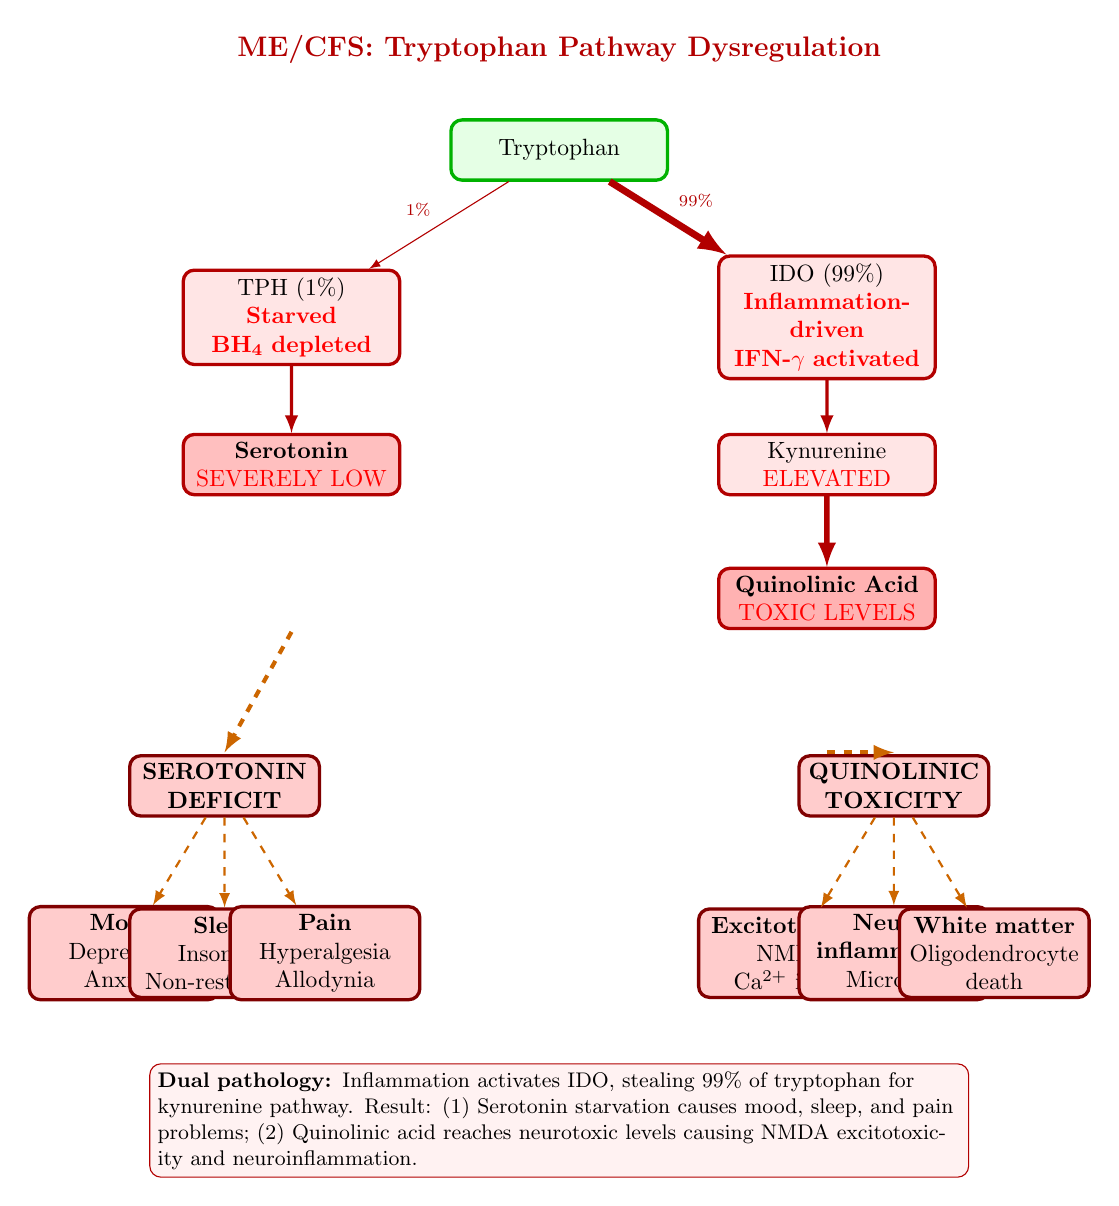
\begin{tikzpicture}[
    node distance=2.5cm,
    scale=0.85, every node/.style={scale=0.85},
    % Styles
    normal/.style={draw=green!70!black, fill=green!10, very thick, rounded corners, text width=3cm, align=center, minimum height=0.9cm},
    impaired/.style={draw=red!70!black, fill=red!10, very thick, rounded corners, text width=3cm, align=center, minimum height=0.9cm},
    pathological/.style={draw=red!50!black, fill=red!20, very thick, rounded corners, text width=2.6cm, align=center, minimum height=0.9cm},
    arrow/.style={-latex, very thick, green!70!black},
    impaired-arrow/.style={-latex, very thick, red!70!black},
    cascade-arrow/.style={-latex, thick, orange!80!black, dashed},
    note/.style={font=\scriptsize\itshape, text width=2.3cm, align=center},
]

% Title
\node[font=\large\bfseries, red!70!black] at (0, 9) {ME/CFS: Tryptophan Pathway Dysregulation};

% TOP: Dysregulated pathway
\begin{scope}[yshift=5cm]
    % Tryptophan
    \node[normal] (trp) at (0, 2.5) {Tryptophan};

    % LEFT: Serotonin - STARVED
    \node[impaired] (tph) at (-4, 0) {TPH (1\%)\\{\color{red}\textbf{Starved}}\\{\color{red}\textbf{BH\textsubscript{4} depleted}}};
    \draw[impaired-arrow, thin] (trp) -- node[above left, font=\scriptsize] {1\%} (tph);

    \node[impaired, fill=red!25] (serotonin) at (-4, -2.2) {\textbf{Serotonin}\\{\color{red}SEVERELY LOW}};
    \draw[impaired-arrow] (tph) -- (serotonin);

    % RIGHT: Kynurenine - HYPERACTIVE
    \node[impaired] (ido) at (4, 0) {IDO (99\%)\\{\color{red}\textbf{Inflammation-driven}}\\{\color{red}\textbf{IFN-$\gamma$ activated}}};
    \draw[impaired-arrow, line width=2.5pt] (trp) -- node[above right, font=\scriptsize] {99\%} (ido);

    \node[impaired] (kyn) at (4, -2.2) {Kynurenine\\{\color{red}ELEVATED}};
    \draw[impaired-arrow] (ido) -- (kyn);

    % Quinolinic acid - TOXIC
    \node[impaired, fill=red!30] (quin) at (4, -4.2) {\textbf{Quinolinic Acid}\\{\color{red}TOXIC LEVELS}};
    \draw[impaired-arrow, line width=2pt] (kyn) -- (quin);
\end{scope}

% BOTTOM: Dual pathology consequences
\begin{scope}[yshift=-4cm]
    % Serotonin deficit consequences (left)
    \node[pathological] (sero-def) at (-5, 2) {\textbf{SEROTONIN}\\  \textbf{DEFICIT}};

    \node[pathological] (mood) at (-6.5, -0.5) {\textbf{Mood}\\Depression\\Anxiety};
    \node[pathological] (sleep) at (-5, -0.5) {\textbf{Sleep}\\Insomnia\\Non-restorative};
    \node[pathological] (pain) at (-3.5, -0.5) {\textbf{Pain}\\Hyperalgesia\\Allodynia};

    \draw[cascade-arrow] (sero-def) -- (mood);
    \draw[cascade-arrow] (sero-def) -- (sleep);
    \draw[cascade-arrow] (sero-def) -- (pain);

    % Quinolinic acid consequences (right)
    \node[pathological] (quin-tox) at (5, 2) {\textbf{QUINOLINIC}\\  \textbf{TOXICITY}};

    \node[pathological] (excito) at (3.5, -0.5) {\textbf{Excitotoxicity}\\NMDA\\Ca\textsuperscript{2+} influx};
    \node[pathological] (neuroinf) at (5, -0.5) {\textbf{Neuro-}\\  \textbf{inflammation}\\Microglia};
    \node[pathological] (white) at (6.5, -0.5) {\textbf{White matter}\\Oligodendrocyte\\death};

    \draw[cascade-arrow] (quin-tox) -- (excito);
    \draw[cascade-arrow] (quin-tox) -- (neuroinf);
    \draw[cascade-arrow] (quin-tox) -- (white);
\end{scope}

% Arrows from pathway to consequences
\draw[cascade-arrow, line width=1.5pt] (-4, 0.3) -- (-5, -1.5);
\draw[cascade-arrow, line width=1.5pt] (4, -1.5) -- (5, -1.5);

% Key point box
\node[draw=red!70!black, fill=red!5, rounded corners, text width=12cm, align=left, font=\small] at (0, -7) {
\textbf{Dual pathology:} Inflammation activates IDO, stealing 99\% of tryptophan for kynurenine pathway. Result: (1) Serotonin starvation causes mood, sleep, and pain problems; (2) Quinolinic acid reaches neurotoxic levels causing NMDA excitotoxicity and neuroinflammation.
};

\end{tikzpicture}
\caption{ME/CFS tryptophan dysregulation causing serotonin deficit and quinolinic acid toxicity.}
\label{fig:tryptophan-mecfs}
\end{figure}


Figures~\ref{fig:tryptophan-normal} and~\ref{fig:tryptophan-mecfs} illustrate tryptophan metabolism dysregulation in ME/CFS. While normally approximately 95\% of tryptophan is metabolized via the kynurenine pathway, inflammation-driven IDO overactivation can substantially increase this proportion. If kynurenine pathway flux increases to approximately 99\% (a plausible estimate based on the magnitude of IDO upregulation observed in inflammatory conditions), this seemingly modest 4 percentage-point shift would dramatically reduce serotonin-available tryptophan from 5\% to 1\%---an 80\% reduction in serotonin precursor availability---while quinolinic acid accumulation reaches toxic levels.

\paragraph{Serotonin Synthesis}
Diversion of tryptophan into the kynurenine pathway reduces availability for serotonin synthesis. This 80\% reduction in available tryptophan for the serotonin pathway may contribute to sleep disturbances, mood symptoms, pain amplification, and cognitive impairment observed in ME/CFS.

\subsubsection{Serotonergic Dysfunction}

Beyond tryptophan diversion, multiple lines of evidence suggest primary serotonergic abnormalities in ME/CFS. These include altered serotonin transporter binding on PET imaging, abnormal responses to serotonergic challenge tests, correlations between serotonin markers and fatigue severity, and variable responses to serotonergic medications.

The serotonergic system's role in regulating sleep, mood, pain perception, and autonomic function makes it a plausible contributor to the multisystem dysfunction of ME/CFS.

\subsubsection{Dopaminergic Dysfunction}

Dopamine abnormalities extend beyond the CSF findings to include reduced dopamine transporter availability in basal ganglia, altered reward processing on functional imaging, blunted dopamine release in response to rewards, and correlation between dopamine markers and motivational symptoms.

The overlap between ME/CFS fatigue and the fatigue observed in Parkinson's disease and other dopaminergic disorders supports a common underlying mechanism.

\subsubsection{Norepinephrine and the Locus Coeruleus}

The locus coeruleus (LC), the primary source of brain norepinephrine, plays critical roles in arousal and sleep-wake regulation, attention and cognitive flexibility, stress responses, and autonomic nervous system modulation.

LC dysfunction could explain the constellation of arousal, attention, and autonomic abnormalities in ME/CFS. Potential mechanisms include neuroinflammation affecting LC neurons, autoantibodies targeting adrenergic receptors, metabolic stress impairing catecholamine synthesis, and chronic stress-induced LC dysregulation.

\subsubsection{GABAergic and Glutamatergic Imbalance}

Magnetic resonance spectroscopy (MRS) studies have revealed abnormalities in the balance between inhibitory (GABA) and excitatory (glutamate) neurotransmission in ME/CFS. These include elevated glutamate/glutamine in some brain regions, reduced GABA concentrations in others, altered glutamate/GABA ratios correlating with symptom severity, and regional variations in neurochemical abnormalities.

This excitatory/inhibitory imbalance could contribute to sensory hypersensitivity, cognitive dysfunction, sleep disturbances, and seizure susceptibility in some patients.

\subsubsection{Cholinergic Dysfunction}

Acetylcholine abnormalities in ME/CFS have received less attention but may contribute to cognitive impairment (particularly memory), autonomic dysfunction (parasympathetic arm), sleep architecture abnormalities, and muscle function.

Autoantibodies against muscarinic acetylcholine receptors have been identified in some ME/CFS patients, providing a potential autoimmune mechanism for cholinergic dysfunction.

\subsection{Sleep Architecture and Inter-Regional Coordination}
\label{sec:sleep-architecture}

Sleep disturbances, particularly unrefreshing sleep despite adequate duration, affect up to 95\% of ME/CFS patients. While subjective complaints are nearly universal, objective polysomnographic findings show more subtle alterations: longer sleep latency, reduced sleep efficiency, increased Stage 3 sleep in adults, and altered sleep microstructure~\cite{Jackson2023sleep}. The paradox---severe subjective sleep dysfunction with modest objective changes---suggests the problem may lie not in sleep duration or stage percentages, but in the \textit{coordination} required to generate and maintain normal sleep architecture.

\subsubsection{Energy Costs of Sleep Architecture Coordination}

Normal sleep architecture requires sophisticated inter-regional brain coordination orchestrated primarily through thalamo-cortical circuits. During non-REM sleep, slow oscillations (~1~Hz) originate in the anterior thalamus and precede neocortical slow oscillations, while sleep spindles (~12--14~Hz) detected in thalamic nuclei precede their neocortical counterparts~\cite{Fernandez2022thalamus}. This sequence---convergent cortical downstates leading thalamic downstates, which then trigger spindles projected back to cortex during the down-to-upstate transition---coordinates memory consolidation across distributed brain regions~\cite{Jiang2024ripples}.

Sleep spindle generation itself is metabolically demanding. Thalamic reticular nucleus (TRN) neurons must generate rhythmic bursts at 12--14~Hz, which requires sustained calcium channel activity, neurotransmitter synthesis and release, and coordinated inhibition of thalamocortical relay neurons. The cortex must then respond appropriately, amplifying spindles and coupling them with hippocampal ripples for memory consolidation. This inter-regional choreography demands substantial ATP and coordinated neurotransmitter systems.

Similarly, REM sleep requires brainstem activation (particularly cholinergic nuclei), thalamic relay, cortical activation approaching waking levels, and simultaneous motor inhibition via brainstem circuits. The transitions between sleep stages---requiring coordinated deactivation of one set of circuits and activation of another---may be particularly energy-intensive.

\begin{hypothesis}[Sleep Architecture Failure Hypothesis]
\label{hyp:sleep-architecture-failure}

In ME/CFS, CNS energy deficits and metabolic dysfunction prevent the sustained inter-regional coordination required for normal sleep architecture, resulting in fragmented sleep microstructure despite adequate total sleep time.

\paragraph{Mechanism.}
The hypothesis proposes that sleep architecture fragmentation in ME/CFS reflects energy-limited coordination failure:

\begin{enumerate}
    \item \textbf{Spindle generation deficit}: Thalamic reticular nucleus neurons cannot sustain the metabolic demands of rhythmic 12--14~Hz burst firing, reducing sleep spindle density and power

    \item \textbf{Slow-wave coordination failure}: Thalamo-cortical circuits cannot maintain synchronized slow oscillations across brain regions, fragmenting slow-wave sleep architecture

    \item \textbf{Stage transition impairment}: The coordinated network reconfiguration required for sleep stage transitions (more demanding than within-stage maintenance) fails preferentially, increasing sleep fragmentation

    \item \textbf{Inter-regional coherence reduction}: EEG coherence between brain regions declines during sleep, reflecting impaired functional connectivity~\cite{Sherlin2011coherence}

    \item \textbf{PEM-induced worsening}: During post-exertional malaise, when CNS energy deficits intensify, sleep architecture fragmentation worsens proportionally
\end{enumerate}

\paragraph{Supporting evidence.}
Jackson et al.~\cite{Jackson2023sleep} meta-analyzed objective sleep data from 801 adults and 477 adolescents with ME/CFS, confirming altered sleep microstructure despite the subjective-objective paradox. Adult patients showed reduced sleep efficiency, altered stage distribution (decreased Stage 2, increased Stage 3), and longer sleep latency---patterns consistent with coordination difficulties rather than simple sleep deprivation.

Sherlin et al.~\cite{Sherlin2011coherence} demonstrated that EEG spectral coherence distinguishes CFS patients from both healthy controls and depressed patients with 100\% accuracy for unmedicated CFS patients. The involvement of bilateral temporal lobes in 9 of 10 coherence factors suggests widespread inter-regional connectivity disruption, supporting the coordination failure hypothesis.

Sleep fragmentation studies show that chronic fragmentation impairs brain energy metabolism to an extent similar to total sleep deprivation, with lower glucose uptake in cortex and hippocampus~\cite{Baud2016fragmentation}. In ME/CFS, the causal arrow may reverse: primary metabolic dysfunction fragments sleep, which further worsens metabolism in a vicious cycle.

\paragraph{Testable predictions.}
\begin{enumerate}
    \item Sleep spindle density and power correlate inversely with ME/CFS symptom severity and biomarkers of CNS dysfunction
    \item Slow-wave sleep fragmentation (not just total SWS percentage) correlates with measures of metabolic dysfunction (e.g., cerebral lactate on MRS)
    \item Sleep architecture fragmentation worsens 24--72 hours post-exertion, tracking PEM time course
    \item Sleep stage transition frequency increases (shorter, more fragmented sleep stages) compared to healthy controls, even when stage percentages appear normal
    \item Inter-regional EEG coherence during sleep is reduced in ME/CFS patients, particularly in frequency bands critical for sleep oscillations (delta, sigma)
    \item Interventions improving cerebral metabolism (e.g., mitochondrial support) improve objective sleep microstructure, not just subjective sleep quality
\end{enumerate}

\paragraph{Treatment implications.}
If sleep architecture failure reflects energy-limited coordination, interventions should target: (1)~circadian optimization---maximizing sleep opportunity during the circadian nadir when sleep pressure is highest; (2)~metabolic support---mitochondrial cofactors (CoQ10, NADH) during evening hours may improve overnight cerebral metabolism~\cite{CastroMarrero2021CoQ10}; (3)~sleep stage-specific support---low-dose gabapentin or pregabalin may reduce thalamo-cortical excitability demands while supporting spindle generation; (4)~glymphatic enhancement---sleep position (lateral decubitus), avoiding late caffeine, and sleep continuity strategies; (5)~pacing-sleep integration---recognizing that sleep quality worsens predictably during PEM can guide activity management.

\paragraph{Limitations.}
This hypothesis has moderate certainty (0.50). No published studies have quantified spindle density or power in ME/CFS with simultaneous metabolic measures. Coherence data exists for waking but not sleep EEG. Alternative explanations include primary brainstem pathology, autonomic dysfunction, or circadian disruption rather than energy limitation. Causality direction remains unclear: does poor metabolism fragment sleep, or does fragmented sleep worsen metabolism?
\end{hypothesis}

\subsection{Glial Cell Dysfunction}
\label{sec:glial}

Beyond neurons and neurotransmitters, glial cells play critical support roles in brain function. Dysfunction in these cells may contribute to the neuroinflammation mentioned in catecholamine synthesis impairment and broader CNS pathology.

\subsubsection{Microglial Activation and Neuroinflammation}

Microglia, the resident immune cells of the central nervous system, have emerged as key players in ME/CFS neuroinflammation. Evidence for microglial activation includes elevated markers in CSF (soluble CD14, chitotriosidase), PET imaging showing increased translocator protein (TSPO) binding in specific brain regions~\cite{Nakatomi2014neuroinflammation}, correlation between neuroinflammatory markers and symptom severity, and persistence of microglial activation years after initial infection.

\textbf{Important note on replication:} The Nakatomi et al.\ 2014 study documenting widespread microglial activation via PET imaging in ME/CFS patients has not been consistently replicated, with later studies showing conflicting results. The certainty of microglial activation as a universal feature of ME/CFS remains medium pending further replication studies.

Chronic microglial activation, when present, can produce sustained release of pro-inflammatory cytokines (IL-1$\beta$, TNF-$\alpha$, IL-6), oxidative stress through reactive oxygen species production, glutamate release contributing to excitotoxicity, disruption of synaptic pruning and plasticity, and blood-brain barrier dysfunction.

\begin{hypothesis}[Glial Maturation Window and Pediatric Recovery]
\label{hyp:glial-maturation-window}

Adolescent ME/CFS patients may benefit from a developmental window during which active microglial remodeling can reset pathological activation states---a mechanism unavailable to adult patients whose glial maturation is complete.

\paragraph{Background: Adolescent Microglial Maturation}

Microglia undergo dramatic functional reorganization during adolescence, performing complex developmental tasks beyond their immune surveillance role. From embryonic neuronal migration to adolescent circuit refinement, immune signaling molecules serve as a common language allowing microglia to modulate brain function in both health and disease~\cite{Dziabis2022microglia}.

Three critical periods define microglial contributions to neural development: embryonic wiring, early postnatal synaptic pruning (peak near birth continuing into late-20s), and adolescent circuit refinement~\cite{Dziabis2022microglia}. During adolescence specifically, microglia mediate experience-dependent synaptic pruning through complement-mediated mechanisms, with C3 binding to CR3 receptors facilitating selective synapse elimination. This process exhibits sex-specific patterns and regional variation, with particularly robust activity in prefrontal cortex and nucleus accumbens~\cite{ScienceAdvances2024adolescent,PMC11758907synapse}.

Crucially, transient microglial deficiency during adolescence---but not adulthood---produces lasting cognitive impairments, identifying adolescence as a sensitive period for prefrontal microglia to act on cognitive development~\cite{ScienceAdvances2024adolescent}. The developmental program requires coordinated microglial activity for proper circuit maturation, with major transitions largely complete by early 20s.

\paragraph{Application to ME/CFS: The Reset Hypothesis}

If ME/CFS involves chronic microglial activation locked in a pro-inflammatory state (as suggested by Nakatomi et al.\ PET findings~\cite{Nakatomi2014neuroinflammation}), then adolescent microglial remodeling may provide a natural mechanism for resolution:

\begin{enumerate}
    \item \textbf{Active turnover}: Adolescent microglia undergo programmed replacement and phenotypic switching as part of circuit refinement, potentially eliminating pathologically activated cells

    \item \textbf{Developmental override signals}: The hormonal and neurochemical milieu of adolescence (BDNF elevation, sex hormones, growth factors) provides strong pro-plasticity signals that may override inflammatory set-points

    \item \textbf{Synaptic reorganization}: Pathological neuroinflammatory states often involve aberrant synaptic connections; adolescent pruning may eliminate these circuits while preserving functional connectivity

    \item \textbf{Adult lock-in}: After developmental windows close (~age 25), microglia lose plasticity for wholesale phenotypic switching, becoming locked in their current activation state without the developmental cues that enable adolescent reset
\end{enumerate}

This framework explains why pediatric ME/CFS shows substantially higher recovery rates (estimated 54--94\% in studies of mild-moderate cases) compared to adult-onset disease where recovery is rare~\cite{Rowe2019pediatric}. The critical variable is not disease duration but rather whether onset occurs before or after completion of microglial maturation.

\paragraph{Testable Predictions}

This hypothesis generates specific, falsifiable predictions:

\begin{enumerate}
    \item \textbf{Age-dependent neuroinflammation}: Longitudinal PET imaging should show declining microglial activation in recovering adolescents but persistent activation in adults with similar disease duration

    \item \textbf{Transition age threshold}: Recovery rates should decline sharply around age 22--25 (completion of prefrontal maturation) rather than showing gradual age-related decline

    \item \textbf{Biomarker trajectories}: CSF inflammatory markers (sCD14, chitotriosidase) should normalize in recovering adolescents but remain elevated in non-recovering adults

    \item \textbf{Microglial turnover markers}: Adolescent patients should show elevated markers of microglial turnover (CSF1R expression, fractalkine signaling) compared to adults

    \item \textbf{Severity interactions}: Hypothesis predicts age matters less if microglial activation is mild (can resolve spontaneously) but becomes critical if activation is severe (requires active remodeling to clear)
\end{enumerate}

\paragraph{Treatment Implications}

If adolescent microglial plasticity enables recovery, then therapeutically inducing similar plasticity in adults might improve outcomes:

\begin{enumerate}
    \item \textbf{CSF-1R inhibitors}: Drugs like PLX5622 or pexidartinib force microglial turnover by depleting existing populations and promoting repopulation from progenitors. This mimics the natural turnover occurring during adolescence, potentially resetting activation states~\cite{MDPI2024microglial}.

    \item \textbf{Fasting-mimicking diets}: Prolonged fasting promotes microglial autophagy and phenotypic switching, potentially enabling transition from pro-inflammatory to surveillance phenotypes without complete depletion

    \item \textbf{BDNF enhancement}: Brain-derived neurotrophic factor drives developmental plasticity; strategies to boost BDNF (exercise within energy envelope, ketogenic diet, certain medications) may partially reopen plasticity windows

    \item \textbf{Timing considerations}: Interventions targeting microglial reset may be most effective in younger adults (under 30) where some residual developmental plasticity remains, with diminishing returns in older patients
\end{enumerate}

\paragraph{Integration with Broader ME/CFS Pathophysiology}

This hypothesis complements rather than contradicts other mechanistic proposals. Microglial activation may be downstream of initial triggers (viral infection, autoantibodies, autonomic dysfunction) while still representing a critical perpetuating factor. The developmental window hypothesis specifically addresses \emph{why recovery patterns differ by age} rather than explaining disease initiation.

The glial maturation window may interact synergistically with other proposed pediatric advantages: immune memory pruning (Hypothesis~\ref{hyp:immune-memory-pruning}, if present), greater HSC regenerative capacity, higher baseline recovery capital (Section~\ref{spec:recovery-capital}), and incomplete epigenetic aging.

\paragraph{Limitations and Uncertainties}

Several important caveats apply:

\begin{enumerate}
    \item The Nakatomi et al.\ microglial activation findings have not been consistently replicated; if microglial activation is not a universal ME/CFS feature, this hypothesis applies only to a subset

    \item The proposed mechanism assumes glial maturation windows close around age 25, but individual variation exists; some adults may retain plasticity longer

    \item Pediatric recovery may reflect multiple mechanisms simultaneously; isolating the specific contribution of microglial remodeling requires longitudinal studies with neuroimaging

    \item CSF-1R inhibitor strategies carry significant risks (meningitis, visual changes) and remain experimental; safety in ME/CFS populations is unknown
\end{enumerate}

\paragraph{Research Priorities}

To test this hypothesis rigorously:

\begin{enumerate}
    \item \textbf{Age-stratified longitudinal neuroimaging}: Serial PET scans in adolescent vs adult ME/CFS tracking microglial activation trajectories over 2--5 years

    \item \textbf{CSF biomarker studies}: Compare inflammatory markers and microglial turnover signatures across age groups and recovery status

    \item \textbf{Preclinical models}: Post-viral fatigue models in adolescent vs adult mice to test whether developmental microglia enable recovery

    \item \textbf{Treatment trials}: Small pilot studies of CSF-1R modulation in carefully selected adult ME/CFS patients with documented microglial activation
\end{enumerate}

This hypothesis provides a mechanistic framework for understanding one component of the pediatric recovery advantage while suggesting potential therapeutic strategies for adult patients.

\end{hypothesis}

\subsubsection{Astrocyte Abnormalities and the Astrocyte Energy Gate}
\label{sec:astrocyte-energy-gate}

Astrocytes perform essential functions including neurotransmitter uptake and recycling, blood-brain barrier maintenance, metabolic support for neurons, synaptic modulation, and ion homeostasis. Astrocyte dysfunction in ME/CFS may contribute to impaired glutamate clearance and excitotoxicity, reduced metabolic support for neurons, blood-brain barrier compromise, and abnormal synaptic transmission. Elevated GFAP (glial fibrillary acidic protein) in some ME/CFS patients suggests astrocyte reactivity, though findings have been inconsistent.

Beyond these recognized roles, astrocytes occupy a uniquely critical position in brain energy metabolism that may constitute a central vulnerability in ME/CFS. The following hypothesis develops this metabolic dimension in detail.

\paragraph{The Astrocyte-Neuron Lactate Shuttle: Normal Physiology}

The brain consumes 20--25\% of the body's glucose despite comprising only 2\% of body mass~\cite{Belanger2011}. A substantial fraction of this energy reaches neurons not as glucose directly, but via the \textbf{astrocyte-neuron lactate shuttle} (ANLS), first described by Pellerin and Magistretti~\cite{Pellerin1994}. In this system, glutamate released during synaptic transmission is taken up by astrocytes via excitatory amino acid transporters (EAATs), triggering astrocytic glucose uptake through GLUT1 transporters and subsequent glycolysis. Astrocytes convert glucose to pyruvate and then to lactate via lactate dehydrogenase A (LDHA), which preferentially catalyzes the pyruvate-to-lactate direction. This lactate is then exported from astrocytes through monocarboxylate transporter 4 (MCT4, a low-affinity, high-capacity exporter) and imported into neurons through MCT2 (a high-affinity importer)~\cite{Pierre2005}. Within neurons, LDHB converts lactate back to pyruvate for oxidative phosphorylation in mitochondria.

This architecture elegantly couples neuronal energy supply to neuronal activity: when a synapse fires, the glutamate released simultaneously signals the local astrocyte to increase energy delivery~\cite{Magistretti2018}. Lactate provides an estimated 30--50\% of neuronal ATP under physiological conditions~\cite{Magistretti2018}, and this fraction likely increases during periods of intense neural activity when neurons' own glycolytic capacity is insufficient.

Several features make this shuttle critical rather than merely supplementary:

\begin{enumerate}
    \item \textbf{Activity coupling:} The glutamate-triggered mechanism ensures energy supply scales with demand at the single-synapse level
    \item \textbf{Metabolic specialization:} Neurons preferentially express LDHB (favoring lactate $\to$ pyruvate) while astrocytes express LDHA (favoring pyruvate $\to$ lactate), creating directional metabolic flow~\cite{Kim2025ANLS}
    \item \textbf{Antioxidant protection:} By outsourcing glycolysis to astrocytes, neurons can direct more glucose through the pentose phosphate pathway for glutathione regeneration, protecting against oxidative damage
    \item \textbf{Signaling function:} Lactate also acts as a signaling molecule via the hydroxycarboxylic acid receptor 1 (HCAR1/GPR81), modulating neuronal excitability and synaptic plasticity~\cite{Magistretti2018}
\end{enumerate}

\paragraph{Important Nuance: Neuronal Metabolic Flexibility}

The classical ANLS model has been refined by recent evidence demonstrating that neurons possess greater metabolic flexibility than originally assumed. Single-cell RNA sequencing studies reveal that neurons express both LDHA and LDHB, not exclusively LDHB~\cite{Kim2025ANLS}. Neurons can directly take up and oxidize glucose, particularly during high-demand states. LDHB-deficient neurons maintain stable energy metabolism under physiological glucose conditions, suggesting compensatory pathways exist.

However, this flexibility has limits. During high-frequency neural activity---precisely the conditions of cognitive exertion---direct neuronal glucose oxidation may prove insufficient, and astrocyte-derived lactate becomes the critical marginal fuel source. This distinction between \emph{basal} sufficiency and \emph{demand-responsive} insufficiency is central to the hypothesis that follows.

\begin{hypothesis}[Astrocyte Energy Gate]
\label{hyp:astrocyte-energy-gate}
We hypothesize that dysfunction in the astrocyte-neuron lactate shuttle creates a \textbf{metabolic bottleneck}---an ``energy gate''---that produces CNS-specific energy failure in ME/CFS while peripheral tissues with direct glucose access remain unaffected.

\paragraph{Three Candidate Mechanisms}

The energy gate may fail at any of three nodes, singly or in combination:

\begin{enumerate}
    \item \textbf{Astrocyte glucose uptake impairment (GLUT1 dysfunction):} Reduced GLUT1 expression or function on astrocytes limits the raw substrate entering the shuttle. GLUT1 deficiency syndrome demonstrates that impaired astrocytic glucose transport causes seizures, cognitive impairment, and brain hypometabolism---features that partially overlap with ME/CFS neurological symptoms. Neuroinflammatory mediators (IL-1$\beta$, TNF-$\alpha$) documented in ME/CFS can downregulate GLUT1 expression.

    \item \textbf{Lactate production impairment (glycolytic defects):} Reactive astrogliosis---documented via elevated GFAP in ME/CFS---involves metabolic reprogramming that may paradoxically impair effective lactate delivery. While reactive astrocytes initially upregulate glycolysis, chronic neuroinflammation shifts astrocyte metabolism toward a state where mitochondrial dysfunction reduces overall metabolic efficiency. Inflammatory cytokines can alter pyruvate dehydrogenase kinase (PDK) activity, disrupting the glycolysis/oxidative phosphorylation balance within astrocytes themselves.

    \item \textbf{Lactate transport impairment (MCT dysfunction):} Downregulation of MCT4 (astrocyte export) or MCT2 (neuronal import) directly restricts lactate flow. This mechanism has the strongest precedent in other neurological diseases: MCT1/MCT4 downregulation reduces neuronal lactate supply by approximately 60\%~\cite{Kim2025ANLS}. In Alzheimer's disease, decreased expression of MCT1, MCT2, and MCT4 is documented. In amyotrophic lateral sclerosis, reduced MCT1 in oligodendrocytes precedes motor neuron degeneration. In temporal lobe epilepsy, MCT2 redistribution and MCT4 reduction are observed in epileptic foci.
\end{enumerate}

\paragraph{Why This Creates Selective Dysfunction}

The energy gate hypothesis explains why CNS function fails while peripheral tissues remain functional:

\begin{itemize}
    \item \textbf{CNS vulnerability:} Neurons depend on the ANLS for a substantial portion of their activity-dependent energy supply. No other cell type in the body has this intermediary requirement for its primary fuel.
    \item \textbf{Peripheral independence:} Skeletal muscle, cardiac muscle, and peripheral tissues express GLUT4 (insulin-responsive) and can directly oxidize glucose without astrocytic intermediation. Hair follicles operate autonomous local Cori cycles, recycling lactate within the follicular unit without CNS coordination.
    \item \textbf{Demand-dependence:} The ANLS is most critical during cognitive exertion (when glutamate release surges trigger proportional lactate demand). This explains why cognitive symptoms worsen with mental effort while resting cognition may remain closer to normal---a hallmark of ME/CFS ``brain fog.''
\end{itemize}

This mechanism connects directly to the selective energy dysfunction hypothesis (Section~\ref{sec:selective-dysfunction}), which predicts that high CNS-dependency ($\alpha$) and high demand-responsiveness ($\rho$) processes should be most impaired. The ANLS provides the \emph{specific molecular mechanism} through which this selective vulnerability operates.

\paragraph{Certainty Assessment}

This hypothesis integrates well-established neuroscience (ANLS physiology: high certainty) with speculative application to ME/CFS (low-to-moderate certainty). No study has directly measured ANLS flux, MCT expression, or astrocyte-specific glycolytic rates in ME/CFS patients. The hypothesis is graded at \textbf{certainty 0.35}: mechanistically plausible, consistent with indirect evidence, but requiring direct experimental validation.
\end{hypothesis}

\paragraph{Supporting Evidence: Brain Lactate Elevation}

While no study has directly assayed ANLS function in ME/CFS, magnetic resonance spectroscopy (MRS) studies provide indirect evidence consistent with impaired brain energy metabolism:

\begin{itemize}
    \item \textbf{7T MRS (2025):} Godlewska et al.~\cite{Godlewska2025MRS} found elevated lactate in the pregenual anterior cingulate cortex (pgACC: 1.52 vs.\ 1.22~mM, $p = 0.003$) and dorsal ACC (dACC) of ME/CFS patients (n=24) compared to healthy controls (n=24), using ultra-high-field 7 Tesla MRS. Notably, ME/CFS and Long COVID patients showed \emph{different} neurochemical profiles despite similar clinical presentations.

    \item \textbf{Whole-brain MRS (2020):} Mueller et al.~\cite{Mueller2020MRS} documented elevated lactate-to-creatine ratios in the right insula, thalamus, and cerebellum (n=15 ME/CFS vs.\ n=15 controls), with brain temperature increases correlated with lactate elevations---suggesting neuroinflammation drives metabolic shifts.

    \item \textbf{Mitochondrial review (2025):} Syed et al.~\cite{Syed2025MitoCFS} synthesize evidence of elevated CSF lactate, impaired ATP synthesis, and increased glycolytic activity in ME/CFS, consistent with oxidative stress and conditions favoring anaerobic metabolism.
\end{itemize}

\begin{warning}[Interpreting Elevated Brain Lactate]
Elevated brain lactate in ME/CFS is consistent with the energy gate hypothesis but does not uniquely support it. At least three interpretations are possible:
\begin{enumerate}
    \item \textbf{ANLS dysfunction:} Lactate accumulates in astrocytes because it cannot be efficiently exported to or utilized by neurons (supports the energy gate hypothesis)
    \item \textbf{Mitochondrial dysfunction:} Neuronal mitochondria cannot oxidize lactate efficiently, causing backpressure (supports a downstream mitochondrial hypothesis)
    \item \textbf{Anaerobic shift:} Increased glycolysis due to hypoperfusion or oxygen limitation produces excess lactate (supports a vascular hypothesis)
\end{enumerate}
These mechanisms are not mutually exclusive and may operate simultaneously. Distinguishing between them requires studies that measure not just lactate levels but lactate \emph{flux} between cellular compartments---technically challenging but feasible with advanced $^{13}$C-MRS techniques.
\end{warning}

\paragraph{Testable Predictions}

The astrocyte energy gate hypothesis generates specific, falsifiable predictions that distinguish it from alternative explanations:

\begin{enumerate}
    \item \textbf{CSF lactate gradient:} If astrocytes produce lactate but neurons cannot utilize it, the CSF lactate/blood lactate ratio should be elevated in ME/CFS (astrocyte-derived lactate accumulating in extracellular space). In mitochondrial disorders affecting the CNS, a CSF/blood lactate ratio $> 0.91$ indicates central origin~\cite{Syed2025MitoCFS}. \\
    \emph{Prediction:} ME/CFS patients will show CSF/blood lactate ratio $> 0.91$, distinguishing CNS-origin lactate from peripheral sources.

    \item \textbf{MCT expression profiling:} Post-mortem or biopsy studies should reveal reduced MCT2 (neuronal) and/or MCT4 (astrocyte) expression in ME/CFS brain tissue, particularly in regions showing functional deficits (prefrontal cortex, anterior cingulate). \\
    \emph{Prediction:} MCT2/MCT4 expression reduced $\geq$30\% vs.\ matched controls.

    \item \textbf{Astrocyte-specific metabolomics:} Single-cell or spatial transcriptomics of ME/CFS brain tissue should show altered expression of glycolytic enzymes (hexokinase, phosphofructokinase, LDHA) and glucose transporters (GLUT1) in astrocytes specifically. \\
    \emph{Prediction:} Astrocyte glycolytic gene expression altered while neuronal oxidative genes remain intact.

    \item \textbf{Exogenous lactate challenge:} If the bottleneck is at the glucose $\to$ lactate step (mechanisms 1 or 2 above), then providing exogenous lactate should partially bypass the gate and improve cognitive function. If the bottleneck is at MCT transport (mechanism 3), exogenous lactate should not help. \\
    \emph{Prediction:} IV sodium lactate infusion during cognitive testing will improve performance in a subgroup of ME/CFS patients.

    \item \textbf{Ketone body bypass:} Ketone bodies ($\beta$-hydroxybutyrate, acetoacetate) enter neurons via MCT2 and are metabolized directly in neuronal mitochondria, bypassing the astrocyte glycolysis step entirely~\cite{Jang2024Ketone}. If the energy gate is at the astrocyte level, ketones should preferentially benefit CNS symptoms. \\
    \emph{Prediction:} Ketogenic diet or exogenous ketone supplementation will improve cognitive symptoms disproportionately to peripheral fatigue symptoms.

    \item \textbf{Activity-dependent worsening:} Since the ANLS is most critical during high neural activity (when glutamate-triggered demand surges), the energy gate should cause greater deficits during cognitive exertion than at rest. \\
    \emph{Prediction:} The difference between resting and task-evoked brain lactate (measured by functional MRS) will be larger in ME/CFS than controls---reflecting both increased demand signaling and impaired supply response.
\end{enumerate}

\paragraph{Treatment Implications}

The energy gate framework suggests several therapeutic strategies, ordered by plausibility and feasibility:

\begin{enumerate}
    \item \textbf{Ketogenic diet or exogenous ketones:} By providing $\beta$-hydroxybutyrate directly to neurons via MCT2, this approach bypasses the astrocyte glycolysis step entirely. The ketogenic diet has established neuroprotective effects in epilepsy (where MCT dysfunction is documented) and emerging evidence in psychiatric disorders associated with brain energy dysfunction~\cite{Jang2024Ketone}. \emph{This represents the most immediately testable intervention.}

    \item \textbf{Exogenous lactate supplementation:} Sodium lactate infusion or oral lactate has shown cognitive benefits in Alzheimer's disease models by restoring hippocampal and CSF lactate concentrations. In ME/CFS, this could bypass impaired astrocyte glycolysis (mechanisms 1--2) but would not help if MCT2 transport is the bottleneck (mechanism 3).

    \item \textbf{MCT upregulation:} Exercise and certain pharmacological agents can upregulate MCT expression. However, exercise intolerance in ME/CFS limits this approach. Pharmacological MCT modulators remain experimental.

    \item \textbf{Anti-neuroinflammatory strategies:} If chronic neuroinflammation drives astrocyte metabolic reprogramming and MCT downregulation, targeting neuroinflammation at its source may restore ANLS function. Low-dose naltrexone (LDN), which modulates microglial activation, could theoretically improve astrocyte metabolic function through reduced neuroinflammatory signaling.

    \item \textbf{Astrocyte-targeted delivery:} Emerging drug delivery technologies using astrocyte-specific targeting (e.g., nanoparticles with GFAP-binding peptides) could deliver metabolic support directly to astrocytes, enhancing glycolytic capacity or MCT expression without systemic effects.
\end{enumerate}

\paragraph{Limitations and Alternative Explanations}

Several important caveats apply to this hypothesis:

\begin{itemize}
    \item \textbf{No direct evidence in ME/CFS:} No study has measured ANLS flux, MCT expression, or astrocyte-specific glycolytic rates in ME/CFS patients. The hypothesis rests entirely on indirect evidence (elevated brain lactate, documented neuroinflammation) and analogy to other neurological conditions.

    \item \textbf{Elevated lactate is ambiguous:} As noted above, elevated brain lactate has at least three interpretations. The ANLS dysfunction interpretation is not uniquely supported by current data.

    \item \textbf{The ANLS itself is debated:} While the ANLS is well-established, its quantitative contribution remains contested. Some evidence suggests neurons can sustain activity through direct glucose oxidation alone, at least under non-demanding conditions~\cite{Kim2025ANLS}. The hypothesis is strongest for high-demand cognitive states.

    \item \textbf{Downstream mitochondrial dysfunction:} Even if lactate reaches neurons normally, impaired neuronal mitochondria (a well-documented finding in ME/CFS~\cite{Syed2025MitoCFS}) would produce similar symptoms. The energy gate and mitochondrial hypotheses are not mutually exclusive but have different treatment implications.

    \item \textbf{GLUT1 paradox:} Recent studies show that astrocyte-specific GLUT1 reduction can \emph{paradoxically improve} brain glucose metabolism, suggesting compensatory mechanisms may complicate predictions based on simple GLUT1 downregulation.

    \item \textbf{Small sample sizes:} The MRS studies supporting brain lactate elevation in ME/CFS have samples of n=15--24, which limits statistical power and generalizability. Larger, multi-site replication studies are needed.
\end{itemize}

For the relationship between the astrocyte energy gate and the broader selective energy dysfunction framework, including formal mathematical treatment and additional predictions, see Section~\ref{sec:selective-dysfunction}, specifically the astrocyte energy gate sub-hypothesis~(\ref{hyp:astrocyte-gate}).

\subsubsection{Oligodendrocyte Function}

Oligodendrocytes produce the myelin sheaths essential for rapid nerve conduction. Potential abnormalities include demyelination contributing to white matter hyperintensities, impaired remyelination capacity, oxidative damage to oligodendrocytes, and disrupted axon-glial signaling.

The white matter changes observed on MRI in ME/CFS patients may reflect oligodendrocyte dysfunction, though the mechanisms remain to be fully elucidated.

\subsubsection{Developmental Context: The Glial Maturation Window}

The discussion of microglial activation in ME/CFS has largely overlooked a critical developmental dimension: the adolescent brain undergoes dramatic microglial reorganization that may explain the differential recovery rates between pediatric and adult patients.

\begin{speculation}[Glial Maturation Window]
\label{spec:glial-maturation}
We propose that adolescent developmental neuroplasticity includes a ``glial maturation window'' during which microglial populations undergo programmed reprogramming that can reset aberrant activation states. This window may explain why pediatric ME/CFS patients recover at dramatically higher rates than adults despite similar initial neuroinflammatory pathology.

\paragraph{Developmental Neuroscience Foundation}
Microglia are not static cells; they undergo profound changes during brain development. During adolescence, several coordinated processes occur:

\textit{Synaptic pruning intensification.} The adolescent brain eliminates approximately 50\% of synapses through microglia-mediated pruning, refining neural circuits~\cite{Paolicelli2011synaptic}. This process peaks around puberty and extends into the early twenties. The pruning machinery requires microglia to transition between surveillance and phagocytic states repeatedly.

\textit{Microglial reprogramming.} As pruning completes, microglia must reset from active phagocytic states to homeostatic surveillance. This reprogramming involves transcriptional reorganization, morphological changes, and functional recalibration. Developmental signals (CSF-1, IL-34, TGF-$\beta$) coordinate this transition.

\textit{Complement system maturation.} The complement cascade (C1q, C3) tags synapses for elimination during development. Complement expression declines after the pruning window closes, potentially reducing the brain's capacity for similar reorganization in adulthood.

\paragraph{Hypothesis: Developmental Pruning Resets Neuroinflammation}
If ME/CFS triggers chronic microglial activation (as suggested by Nakatomi et al.'s PET data, pending replication), adolescent patients may have an inherent advantage: the ongoing developmental pruning program could ``sweep away'' aberrantly activated microglia along with the synapses being eliminated. The same signals that coordinate normal developmental pruning may force activated microglia to either reset to surveillance phenotypes or be replaced by newly differentiated cells from progenitor pools.

In adults, this developmental program is complete. Microglia that shift to pro-inflammatory phenotypes lack the developmental signals that would trigger reset. Without external intervention, activated microglia may persist indefinitely, maintaining chronic neuroinflammation.

\paragraph{Testable Predictions}
This hypothesis generates several falsifiable predictions:
\begin{enumerate}
    \item PET imaging with TSPO ligands should show higher microglial activation in adult ME/CFS patients compared to pediatric patients of similar disease duration and severity.
    \item Pediatric ME/CFS patients who recover should show normalization of microglial markers over time, while non-recovering patients (and adults) should show persistent activation.
    \item The recovery rate differential should diminish for patients whose onset occurs after the developmental window closes (early twenties).
    \item Biomarkers of developmental pruning activity (complement proteins, synaptic markers in CSF) should correlate with recovery probability in pediatric patients.
\end{enumerate}

\paragraph{Therapeutic Implications}
If the glial maturation window hypothesis is correct, therapeutic strategies could aim to artificially induce microglial turnover or reprogramming in adults:

\textit{CSF-1R inhibition.} Colony-stimulating factor 1 receptor (CSF-1R) is essential for microglial survival. CSF-1R inhibitors (such as PLX5622 in animal models, or pexidartinib which is FDA-approved for tenosynovial giant cell tumors) can deplete microglia, which then repopulate from CNS progenitors in a potentially ``reset'' state. Preclinical studies in mouse models of neuroinflammation show that microglial depletion and repopulation can resolve chronic neuroinflammatory states~\cite{Elmore2014csf1r}. However, global microglial depletion carries risks, and clinical translation for ME/CFS would require careful safety evaluation.

\textit{Fasting-mimicking interventions.} Prolonged fasting or fasting-mimicking diets have been shown to promote microglial turnover and reduce neuroinflammation in animal models~\cite{Choi2018fasting}. The mechanisms may involve autophagy induction, stem cell activation, and metabolic reprogramming. While speculative for ME/CFS, dietary interventions represent a lower-risk approach to test the hypothesis.

\textit{BDNF and neuroplasticity promoters.} Brain-derived neurotrophic factor (BDNF) promotes neural plasticity and may influence microglial phenotype. Interventions that increase BDNF (exercise in those who tolerate it, certain antidepressants, photobiomodulation) could theoretically support glial homeostasis, though evidence in ME/CFS is limited.

\paragraph{Research Priorities}
Priority research to test this hypothesis should include:
\begin{enumerate}
    \item Comparative PET neuroimaging study of pediatric versus adult ME/CFS patients using second-generation TSPO ligands
    \item Longitudinal CSF biomarker study tracking microglial activation markers (sTREM2, chitotriosidase) in pediatric patients through recovery or chronification
    \item Preclinical studies of CSF-1R inhibition in post-viral fatigue animal models
    \item Safety and feasibility studies of fasting-mimicking protocols in stable ME/CFS patients
\end{enumerate}

\paragraph{Limitations}
This hypothesis rests on uncertain foundations. The Nakatomi et al.\ PET findings require replication. The developmental neuroscience of microglial reprogramming is still being elucidated, and translation from animal models to human disease is uncertain. The hypothesis also does not explain why some pediatric patients fail to recover, though this could reflect variation in the timing or completeness of developmental processes.

Despite these limitations, the glial maturation window hypothesis provides a testable framework for understanding the pediatric recovery advantage through a neuroimmune lens. If supported by evidence, it would suggest specific therapeutic targets for inducing microglial reset in adult patients. A comparative study of pediatric versus adult ME/CFS patients (Section~\ref{sec:pediatric-adult-study}) could help test predictions of this hypothesis.
\end{speculation}

\subsubsection{Post-Viral CNS Reprogramming}

The preceding sections document microglial activation, astrocyte dysfunction, and neuroinflammatory cascades in ME/CFS. A critical question is why these states persist long after the triggering infection resolves. Emerging evidence from trained immunity research suggests that a single viral infection can permanently alter glial cell function through epigenetic mechanisms.

\begin{speculation}[Post-Viral CNS Reprogramming Hypothesis]
\label{spec:post-viral-cns-reprogramming}

Viral infection causes persistent epigenetic reprogramming of astrocytes and microglia, creating a lasting shift in CNS metabolism that persists long after viral clearance. This mechanism---analogous to ``trained immunity'' in peripheral innate immune cells---may explain why ME/CFS becomes chronic following acute infection.

\paragraph{Trained immunity and epigenetic memory.}
Trained immunity refers to the capacity of innate immune cells to develop long-lasting functional memory following initial stimulation~\cite{Humer2025TrainedImmunityMECFS}. Unlike adaptive immune memory mediated by lymphocyte clonal expansion, trained immunity operates through persistent epigenetic modifications---particularly histone marks such as H3K4me1 and H3K27ac at inflammatory gene promoters---that prime cells for enhanced responses to subsequent stimuli. Humer et al.\ advocate trained immunity as a contributing factor to ME/CFS pathogenesis, proposing that post-infectious epigenetic reprogramming of innate immune cells produces a hyperresponsive phenotype that sustains chronic inflammation~\cite{Humer2025TrainedImmunityMECFS}.

\paragraph{Microglial epigenetic reprogramming.}
Wendeln et al.\ demonstrated in a landmark \textit{Nature} study that peripheral inflammatory stimuli induce long-lasting epigenetic reprogramming of brain microglia~\cite{Wendeln2018InnateImmuneMemoryBrain}. Trained microglia develop enhanced H3K4me1 marks at inflammatory gene loci that persist for months after the initial stimulus and exacerbate subsequent neurological pathology. This immune memory operates through metabolic reprogramming: activated microglia shift from oxidative phosphorylation to aerobic glycolysis, and this metabolic phenotype becomes epigenetically stabilized~\cite{Nirakis2025MetabolicRegulationMicroglial}. The persistence of these marks means that a single viral infection could establish a ``new normal'' of microglial function that outlasts the infection by years.

\paragraph{Viral reprogramming of glial metabolism.}
Rodrigues et al.\ demonstrate that neurotropic viruses---including SARS-CoV-2, HIV-1, and Zika virus---directly infect astrocytes and microglia, causing metabolic shifts from oxidative phosphorylation to glycolysis with consequent NLRP3 inflammasome activation~\cite{Rodrigues2025ViralReprogrammingGlialMetabolism}. This metabolic reprogramming is not merely a transient response to active infection; it persists because the glycolytic shift triggers epigenetic modifications that stabilize the pro-inflammatory phenotype. The result is a self-sustaining cycle: viral infection $\rightarrow$ metabolic shift $\rightarrow$ epigenetic stabilization $\rightarrow$ chronic neuroinflammation.

This mechanism has direct relevance to the astrocyte energy gate hypothesis (Section~\ref{sec:astrocyte-energy-gate}): if viral infection reprograms astrocytes to favor glycolysis over oxidative phosphorylation, lactate production via the astrocyte-neuron lactate shuttle may be disrupted. Astrocytes locked in a glycolytic-inflammatory phenotype may consume glucose for their own inflammatory signaling rather than converting it to lactate for neuronal use.

\paragraph{Broader epigenetic landscape in ME/CFS.}
Apostolou and Ros\'en document over 12,000 altered CpG methylation sites in ME/CFS patients, with particular enrichment at immune and metabolic gene loci~\cite{Apostolou2024EpigeneticReprogrammingMECFS}. They propose that latent herpesviruses (particularly EBV) employ long-term epigenetic strategies that may permanently alter host cell function. Complementing this, Iu et al.\ demonstrate that CD8$^+$ T cells in ME/CFS exhibit epigenetic predisposition toward terminal exhaustion, with exhaustion markers upregulated following exercise challenge~\cite{Iu2024TranscriptionalReprogrammingCD8}---linking immune reprogramming directly to post-exertional malaise.

\paragraph{Testable predictions.}
\begin{enumerate}
    \item Post-infectious ME/CFS patients should show distinct microglial epigenetic signatures (elevated H3K4me1/H3K27ac at inflammatory loci) compared to gradual-onset patients, detectable via CSF-derived microglia or post-mortem analysis
    \item Astrocyte metabolic profiles (measurable via MRS glutamate/glutamine ratios) should differ between post-viral and non-viral ME/CFS subtypes
    \item Epigenetic modifiers targeting trained immunity (e.g., histone methyltransferase inhibitors, mTOR pathway modulators) should preferentially benefit post-infectious ME/CFS
    \item Early antiviral or anti-inflammatory intervention during acute infection should reduce ME/CFS incidence by preventing epigenetic stabilization
    \item CSF cytokine profiles should show trained immunity signatures (enhanced IL-6, TNF-$\alpha$ responses to ex vivo stimulation) in post-infectious but not gradual-onset patients
\end{enumerate}

\paragraph{Treatment implications.}
If post-viral CNS reprogramming drives chronic ME/CFS, therapeutic strategies should target epigenetic reversal rather than symptomatic suppression: (1)~epigenetic modifiers that can cross the BBB and reset microglial histone marks; (2)~metabolic interventions that shift astrocytes back from glycolysis to oxidative phosphorylation; (3)~microglial depletion and repopulation via CSF-1R inhibition (see Section~\ref{spec:glial-maturation}), which may generate microglia without the trained immunity epigenetic marks; (4)~early intervention protocols during acute viral illness to prevent epigenetic stabilization.

\paragraph{Limitations.}
This hypothesis has certainty 0.40. No study has directly measured trained immunity epigenetic marks in ME/CFS patient microglia. The evidence is synthesized from trained immunity research in neurodegenerative diseases~\cite{Wendeln2018InnateImmuneMemoryBrain,Zhang2025TrainedImmunityNeurological}, viral glial reprogramming~\cite{Rodrigues2025ViralReprogrammingGlialMetabolism}, and ME/CFS epigenetic profiling~\cite{Apostolou2024EpigeneticReprogrammingMECFS}. The mechanism may not explain gradual-onset ME/CFS without clear viral trigger. Individual variation in epigenetic susceptibility and viral tropism could produce heterogeneous responses.
\end{speculation}

\subsection{Integrated Neuroinflammatory Cascade Model}

The diverse neurological abnormalities documented in ME/CFS—neurotransmitter depletion, microglial activation, autonomic dysregulation—may not be independent pathologies but rather interconnected components of a unified cascade originating from the central nervous system.

\begin{hypothesis}[Neuroinflammatory Cascade: From CNS to Peripheral Symptoms]
\label{hyp:cascade-neuroinflammatory}

We propose an integrated cascade model in which neuroinflammatory dysfunction serves as an upstream driver of both central and peripheral ME/CFS pathology~\cite{MCMC2024Neurometabolic,NIH2024MECFSRoadmap}:

\paragraph{Cascade pathway}

\textit{Infection or immune challenge:} Initial infection (EBV, enterovirus, or other trigger) activates innate immunity and produces transient CNS inflammation through multiple routes (direct viral CNS invasion, systemic inflammatory cytokines crossing BBB, peripheral immune cell infiltration).

\textit{Sleep disruption and impaired glymphatic clearance:} Acute neuroinflammation disrupts sleep architecture and circadian regulation. Critically, sleep loss impairs the glymphatic system---the brain's waste clearance mechanism dependent on aquaporin-4 water channels in astrocytes. During sleep, the glymphatic system increases interstitial space and clears accumulated metabolic byproducts. Without adequate sleep, toxic protein aggregates (misfolded proteins, amyloid, tau) accumulate in the parenchyma.

\textit{Persistent neuroinflammation and microglial priming:} Impaired glymphatic clearance allows accumulation of pathogen-associated molecular patterns (PAMPs) and damage-associated molecular patterns (DAMPs), which sustain microglial activation. Primed microglia become hyperresponsive to subsequent stimuli, producing exaggerated cytokine responses (IL-1$\beta$, TNF-$\alpha$, IL-6) to minor perturbations.

\textit{Central neurotransmitter depletion:} Sustained neuroinflammation and microglial activation reduce synthesis of catecholamines and serotonin through multiple mechanisms: (1) inflammatory cytokines inhibit tyrosine hydroxylase and tryptophan hydroxylase expression, (2) oxidative stress from microglia-derived reactive oxygen species damages the enzymes and their cofactors, (3) catecholamine reuptake is impaired by cytokine-mediated transporter dysfunction, (4) metabolic depletion reduces substrate availability for neurotransmitter synthesis.

\textit{Central neurological dysfunction:} Catecholamine and serotonin depletion produce multiple consequences: effort-related dysfunction (hyperdopaminergic responses to exertion trigger rapid catecholamine depletion, producing the post-exertional symptom surge characteristic of PEM), cognitive dysfunction (prefrontal catecholamine depletion impairs attention, working memory, and executive function), and sickness behavior activation (inflammatory cytokines and depleted monoamines trigger the evolutionarily conserved sickness behavior program---fatigue, anhedonia, reduced activity tolerance—which is protective but becomes maladaptive when persistent).

\textit{Autonomic dysregulation:} Depleted brainstem catecholamine systems (particularly the locus coeruleus) and impaired parasympathetic signaling (reduced acetylcholine availability) produce observable autonomic dysfunction: reduced heart rate variability, abnormal blood pressure regulation (orthostatic intolerance, POTS-like features), impaired vagal anti-inflammatory signaling, and loss of normal sympatho-parasympathetic balance.

\textit{Peripheral symptom manifestation:} The combination of catecholamine depletion, sickness behavior, and autonomic dysregulation produce the characteristic ME/CFS symptom constellation: profound fatigue, post-exertional malaise, cognitive dysfunction, pain, and orthostatic intolerance.

\textit{Metabolic dysfunction and amplification loop:} Forced inactivity (due to neurologically-driven inability to exert), medication effects (many treatments deplete catecholamines further), and chronic systemic inflammation drive metabolic dysfunction: mitochondrial ATP production declines, lactate accumulation increases, metabolic flexibility is impaired. Metabolic dysfunction itself produces inflammatory signals (lactate, damaged mitochondria) that amplify neuroinflammation. This creates a positive feedback loop: neuroinflammation → peripheral symptoms → reduced activity → metabolic dysfunction → amplified neuroinflammation.

\paragraph{Key assumptions}

This cascade model rests on a critical causal assumption: \textbf{central nervous system dysfunction is causally primary}, driving peripheral manifestations rather than resulting from them. Alternative causal hierarchies are biologically plausible. For example, if primary immune dysfunction (impaired viral clearance, B cell dysfunction, autoantibody production) drives disease, peripheral pathology would come first, and CNS involvement would be secondary. Similarly, if metabolic dysfunction (mitochondrial ATP depletion, lactate accumulation) is the primary driver, neurological changes might reflect metabolic rather than neuroinflammatory etiology. These alternative models would predict different therapeutic hierarchies and treatment response patterns. The cascade model specifically predicts that CNS-targeted interventions (sleep restoration, microglial modulation, catecholamine restoration) should be foundational to treatment, whereas peripheral organ-targeted therapy (cardiac drugs for POTS, antivirals for presumed viral persistence) would be less effective if peripheral dysfunction is secondary. Testing this assumption requires comparative treatment trials: if CNS-first approaches produce superior outcomes to periphery-first approaches in randomized trials, the cascade model's assumption is supported; if peripheral approaches are equally or more effective, the causality assumption is questioned.

\paragraph{Key implications of this model}

This cascade model positions \textit{central neurological dysfunction as upstream of peripheral symptoms} rather than secondary to them. If correct, it suggests fundamentally different therapeutic strategies than those targeting peripheral organs:

\begin{enumerate}
    \item \textbf{Sleep is disease-modifying:} Sleep disruption perpetuates the cascade by impairing glymphatic clearance. Interventions that restore sleep (sleep hygiene, low-dose sedating agents, circadian restoration) may directly interrupt neuroinflammation, not merely improve symptoms.

    \item \textbf{Microglial modulation is central:} Interventions targeting microglial activation (CSF-1R inhibition as discussed in Section~\ref{spec:glial-maturation}, fasting-mimicking diets promoting microglial turnover) may provide disease-modifying benefit.

    \item \textbf{Catecholamine restoration requires CNS targeting:} Peripheral catecholamine replacement (standard treatments for POTS) may be ineffective if the primary problem is CNS depletion and impaired synthesis. Centrally-acting drugs (L-DOPA, levodopa with carbidopa to cross BBB, dopamine agonists) might be more effective than peripheral sympathomimetics.

    \item \textbf{Breaking the positive feedback loop is critical:} Preventing forced inactivity through appropriate pacing prevents the metabolic dysfunction that amplifies neuroinflammation. This aligns with clinical observations that strict pacing produces better long-term outcomes than progressive exercise approaches.
\end{enumerate}

\end{hypothesis}

\subsection{Post-Exertional Malaise and the Kindling Hypothesis}

The clinical observation that each crash lowers the threshold for the next crash---that activities previously tolerated trigger worse symptoms as disease progresses---parallels a phenomenon well-established in neurology: kindling.

\begin{hypothesis}[Post-Exertional Malaise Kindling and Progressive Sensitization]
\label{hyp:pem-kindling-sensitization}

We propose that PEM represents a form of neurobiological kindling in which repeated neuroinflammatory activation progressively lowers the threshold for triggering symptom exacerbations~\cite{Nakatomi2014neuroinflammation,MCMC2024Neurometabolic,NIH2024MECFSRoadmap}.

\paragraph{Kindling mechanism}

\textit{Initial exertion:} An activity requiring catecholamine-dependent effort (physical exertion, cognitive demanding tasks, emotional stress, or infection) triggers acute catecholamine release from depleted stores. If CNS catecholamine availability is already compromised by neuroinflammation, even a modest exertion produces a substantial percentage depletion of the remaining pool.

\textit{Threshold and collapse:} The neuronal systems dependent on catecholamines cannot function effectively once availability drops below a critical threshold. This produces the acute collapse characteristic of PEM: sudden fatigue, cognitive shutdown, pain, orthostatic intolerance.

\textit{Microglial priming from exertion:} The acute catecholamine depletion and cellular stress from exertion act as a DAMP (damage-associated molecular pattern), priming already-activated microglia further. Additionally, the metabolic disruption during exertion (increased lactate, ROS production, cellular damage) provides more inflammatory signals.

\textit{Lowered threshold post-exertion:} Following a PEM episode, microglial priming increases. The threshold for the next crash ($T_2$) is lower than the threshold before ($T_1$): activities that previously could be tolerated now trigger crashes because less catecholamine depletion is required to cross the now-lower threshold.

\textit{Progressive sensitization:} With repeated PEM episodes, this kindling process repeats: T(n) < T(n-1). Each crash further primes microglia, further sensitizes the system, further lowers the threshold. Over time, trivial activities trigger crashes. Some patients reach a state where standing, conversations, or eating triggers symptoms.

\paragraph{Quantitative model}

Let T(n) be the activity threshold at time n (e.g., kcal expended before triggering PEM):

\begin{itemize}
    \item Initial state: T(0) = baseline (e.g., 500 kcal before crash triggered)
    \item First crash: Exertion approaching T(0) triggers depletion below critical threshold, PEM occurs, microglial priming increases by factor $\alpha$
    \item Post-crash state: T(1) = T(0) / $\alpha$ (threshold lowered by priming factor)
    \item Second crash: Exertion of magnitude T(1) triggers symptoms; microglial priming increases further
    \item Recursive decline: T(n) = T(n-1) / $\alpha$ = T(0) / $\alpha$\textsuperscript{n}
\end{itemize}

With priming factor $\alpha$ = 1.5 (a 50\% lowering per crash), the progression would be:
T(0) = 500 kcal → T(1) = 333 kcal → T(2) = 222 kcal → T(5) = 65 kcal

\textit{Note on model parameters:} The priming factor $\alpha$ and the specific threshold values shown (500, 333, 222, 65 kcal-equivalent) are illustrative only and not empirically derived. The actual value of $\alpha$ is unknown and likely varies substantially between patients depending on baseline microglial activation state, genetic factors affecting neuroinflammatory response, and disease duration. These example values are presented solely to demonstrate the exponential relationship between crash number and threshold reduction. Any quantitative application of this model requires direct empirical measurement of individual patient thresholds over time.

\paragraph{Clinical and prognostic implications}

This kindling model explains several critical clinical observations:

\textit{Crash begets crashes:} The threshold-lowering effect means that a single exertion event doesn't just cause temporary symptoms but permanently alters the disease trajectory by priming for future crashes. This has profound implications for disease modification.

\textit{Strict pacing prevents further sensitization:} If exertions are carefully limited to sub-threshold levels (well below the current threshold T(n)), no additional crash occurs and microglial priming does not increase further. This prevents the recursive threshold decline. In this framework, strict pacing is not merely symptomatic management but disease-modifying---it halts the progressive sensitization process. Patients who maintain strict pacing may stabilize at their current threshold; those who allow repeated crashes will worsen progressively.

\textit{Infections produce major priming events:} Each infection represents a major immunological and neuroinflammatory event. In the kindling framework, infection reactivation (EBV, HHV-6) or new infection produces substantial microglial priming, equivalent to multiple PEM episodes. This explains the clinical pattern that infections mark step-wise deterioration in ME/CFS---they reset the kindling process upward.

\textit{Recovery becomes progressively harder:} In early disease (low n, high T(n)), exertions are still available that don't trigger crashes; nervous system can gradually rebuild reserves. As kindling progresses (high n, low T(n)), almost all activities trigger crashes; positive feedback dominates. Recovery requires not just stopping new crashes but actively deprimming microglia. This becomes increasingly difficult as the patient becomes more sensitized.

\textit{Early intervention is critical:} At disease onset (low n), the threshold has not dropped far. Early application of strict pacing and anti-neuroinflammatory interventions could potentially prevent the recursive decline. Later, after many crashes, the threshold has dropped far and recovery requires intensive deprimming. This suggests that early aggressive management (e.g., immediate bed rest, microglial suppression, infection prevention, metabolic support) following disease onset might prevent chronic progression, whereas late intervention faces an already-sensitized nervous system.

\paragraph{Treatment implications}

If the kindling hypothesis is correct:

\textit{Strict pacing is disease-modifying:} Currently, pacing is recommended as symptomatic management. The kindling model suggests it should be recognized as disease-modifying---directly interrupting the progressive sensitization process. Patients who maintain pacing avoid further kindling and preserve their remaining threshold. Those who do not may see progressive functional decline.

\textit{Blocking new kindling triggers is critical:} Infections are major microglial priming events. Preventing infections (FFP2 masking in high-transmission periods, prophylactic antivirals if options become available, rapid treatment of infections) becomes disease-modifying therapy because it prevents the threshold-lowering spike from infection-induced microglial activation.

\textit{Active deprimming requires intervention:} Merely halting new crashes (pacing) prevents further decline but doesn't reverse existing kindling. If the hypothesis is correct, therapies that actively reverse microglial priming (CSF-1R inhibition to deplete and regenerate microglia, fasting-promoting interventions to reset glial metabolism, neuroplasticity-promoting therapies like low-dose BDNF or photobiomodulation) might restore threshold to baseline over time.

\paragraph{Falsification criteria}

The kindling hypothesis makes specific predictions that can be empirically refuted. The hypothesis would be falsified by:

\begin{enumerate}
    \item \textbf{Absence of cumulative threshold reduction:} If longitudinal studies controlling for overall disease progression show that repeated PEM episodes do not produce measurable cumulative lowering of subsequent thresholds, the kindling mechanism would be unsupported. For example, if two patient groups with similar baseline disease duration and severity show the same activity threshold despite vastly different crash histories, kindling-mediated threshold reduction would be unlikely.

    \item \textbf{Reversibility of thresholds after prolonged rest:} If extended rest periods (3+ months) with strict activity limitation consistently restore pre-crash thresholds to baseline levels, this would suggest sensitization is reversible rather than kindling-like. True kindling produces cumulative, largely irreversible changes; reversible sensitization would point to different mechanisms (e.g., temporary glial activation without permanent priming).

    \item \textbf{Absence of microglial correlates:} If microglial markers (CSF1-R positron emission tomography imaging, cerebrospinal fluid inflammatory mediators, or microglial activation markers) show no correlation with PEM crash history, threshold reduction, or disease severity, this would weaken the proposed microglial mechanism. Conversely, finding these markers elevated equally in patients with few versus many crashes would suggest microglial involvement is secondary rather than driving kindling.

    \item \textbf{Lack of threshold reduction with infection-equivalent priming:} If experimental immune activation (e.g., viral challenge or endotoxin administration) that triggers robust microglial and systemic inflammatory responses does not produce measurable threshold lowering in animal models of ME/CFS-like disease, the kindling mechanism would be questionable.
\end{enumerate}

\end{hypothesis}

\section{Autonomic Nervous System Dysfunction}
\label{sec:ans-pathophysiology}

Autonomic dysfunction is nearly universal in ME/CFS and contributes substantially to disability. The NIH deep phenotyping study provided quantitative documentation of specific autonomic abnormalities~\cite{walitt2024deep}.

\subsection{Sympathetic vs. Parasympathetic Imbalance}
\label{sec:autonomic-imbalance}

\subsubsection{Heart Rate Variability Studies}

Heart rate variability (HRV) provides a non-invasive window into autonomic function. The NIH study documented significantly diminished HRV in PI-ME/CFS patients compared to controls~\cite{walitt2024deep}. These changes included reduced overall variability (lower standard deviation of NN intervals or SDNN, reflecting decreased overall autonomic modulation), diminished high-frequency power (reduced HF-HRV, specifically reflecting decreased parasympathetic or vagal activity), altered low-frequency power (changes in LF-HRV, influenced by both sympathetic and parasympathetic activity), and abnormal LF/HF ratio (suggesting sympathovagal imbalance).

\paragraph{Clinical Implications of Reduced HRV}
Diminished HRV in ME/CFS correlates with greater fatigue severity (Escorihuela et al., n=45: RMSSD p=0.027, HFnu p=0.007~\cite{Escorihuela2020hrv}), worse orthostatic intolerance, impaired cognitive function, reduced exercise capacity, and poorer quality of life.

Low HRV is also an independent predictor of cardiovascular morbidity and mortality in other populations, raising concerns about long-term cardiovascular outcomes in ME/CFS.

\subsubsection{Baroreflex Sensitivity}

The baroreflex maintains blood pressure stability through rapid adjustments in heart rate and vascular tone. The NIH study found diminished baroreflex cardiovagal gain in ME/CFS patients~\cite{walitt2024deep}, indicating impaired ability to modulate heart rate in response to blood pressure changes, reduced parasympathetic responsiveness, delayed cardiovascular adaptation to postural changes, and vulnerability to orthostatic stress.

\paragraph{Baroreflex Testing Methods}
Several methods assess baroreflex function. Spontaneous baroreflex analysis calculates the relationship between spontaneous blood pressure and R-R interval fluctuations. The Valsalva maneuver assesses heart rate and blood pressure responses to standardized straining. Neck suction or pressure directly stimulates carotid baroreceptors, while pharmacological methods use vasoactive drugs to manipulate blood pressure.

\subsubsection{Evidence for Decreased Parasympathetic Activity}

Multiple lines of evidence converge on parasympathetic (vagal) dysfunction as a central feature of ME/CFS autonomic abnormalities. Reduced HRV high-frequency power provides a direct measure of cardiac vagal modulation. Diminished baroreflex sensitivity, which is primarily mediated by vagal mechanisms, further supports this dysfunction. Pupillary abnormalities reveal altered pupil responses to light (parasympathetically mediated), while gastrointestinal dysmotility reflects vagal nerve dysregulation of gut function. Additionally, reduced respiratory sinus arrhythmia indicates impaired vagally mediated heart rate variation with breathing.

The NIH study explicitly concluded that the autonomic findings indicated ``decreased parasympathetic activity''~\cite{walitt2024deep}, providing a unifying explanation for many ME/CFS symptoms.

\subsubsection{Sympathetic Nervous System Abnormalities}

While parasympathetic dysfunction is prominent, sympathetic abnormalities also occur. Resting sympathetic overactivity manifests as elevated norepinephrine spillover and increased muscle sympathetic nerve activity. Despite this elevated baseline, sympathetic reactivity is impaired, showing blunted responses to stressors. Regional sympathetic dysfunction produces variable activation across different vascular beds, while catecholamine dysregulation affects synthesis, release, and clearance.

\textbf{Reconciling central vs.\ peripheral norepinephrine:} An apparent contradiction exists between reduced central (CNS) norepinephrine documented in CSF~\cite{walitt2024deep} and elevated peripheral norepinephrine spillover. This likely reflects compartmentalization: central noradrenergic systems (locus coeruleus, brain norepinephrine) are separate from peripheral sympathetic nervous system activity. One proposed mechanism is that central deficiency could plausibly impair the brain's regulation of the sympathetic nervous system, leading to dysregulated peripheral sympathetic output---elevated at rest but unable to respond appropriately to challenges. This dissociation between central and peripheral catecholamine compartments is well-established in autonomic physiology.

The combination of elevated baseline sympathetic activity with reduced reactivity creates a rigid, poorly adaptive autonomic system unable to respond appropriately to physiological challenges.

\subsection{Mechanisms of Orthostatic Intolerance}
\label{sec:orthostatic-mechanisms}

Orthostatic intolerance (OI) affects an estimated 70--90\% of ME/CFS patients and manifests as postural orthostatic tachycardia syndrome (POTS), neurally mediated hypotension (NMH), orthostatic hypotension (OH), or combinations of these conditions.

Dysautonomia and POTS are components of the ``Septad'' framework of frequently co-occurring conditions in ME/CFS (Section~\ref{sec:septad}). Small fiber neuropathy, another Septad component, may underlie autonomic dysfunction in a subset of patients, emphasizing the need for comprehensive evaluation of these interrelated pathophysiologies.

\subsubsection{Blood Volume Abnormalities}

Reduced blood volume is well-documented in ME/CFS and contributes to orthostatic intolerance~\cite{Streeten1998blood}. Streeten and Bell documented that red blood cell mass was significantly reduced (p<0.001) in 93.8\% of female patients and 50\% of male patients, with plasma volume subnormal in 52.6\%. This total blood volume decrease compromises cardiovascular reserve through mechanisms possibly involving renin-angiotensin-aldosterone system dysfunction, reduced erythropoietin, or increased capillary permeability.

Hypovolemia reduces cardiac preload, compromising stroke volume and cardiac output, particularly during orthostatic stress.

\subsubsection{Vascular Dysfunction}

Multiple vascular abnormalities contribute to orthostatic intolerance. Impaired venoconstriction reduces the ability to mobilize venous blood during standing, leading to excessive venous pooling as blood accumulates in dependent vessels. Arterial dysregulation produces abnormal resistance vessel responses, while endothelial dysfunction impairs nitric oxide bioavailability.

\subsubsection{Adrenergic Receptor Dysfunction}

Abnormalities in adrenergic receptor function may explain some autonomic symptoms. Beta-adrenergic receptor autoantibodies have been identified in subsets of ME/CFS patients~\cite{Loebel2016} and may either activate or block receptors. Loebel et al.\ found that 29.5\% of ME/CFS patients (n=268) had elevated autoantibodies against $\beta$2, M3, and/or M4 receptors. Antibodies against $\beta$2 adrenergic and M3 muscarinic receptors (both vasodilators) could explain vasoconstriction and hypoxemia observed in ME/CFS. Alpha-adrenergic abnormalities produce altered vasoconstrictor responses, while receptor desensitization may result from chronic catecholamine exposure downregulating receptors. Additionally, post-receptor signaling defects in G-protein coupling or second messenger systems may contribute to dysfunction.

\subsubsection{Renin-Angiotensin-Aldosterone System}

The RAAS regulates blood volume and pressure through sodium and water retention, vasoconstriction, and sympathetic activation.

Abnormalities in ME/CFS may include reduced aldosterone response to orthostatic stress, impaired renin secretion, altered angiotensin II sensitivity, and inappropriate natriuresis.

\section{Peripheral Nervous System}
\label{sec:peripheral-nervous}

\subsection{Small Fiber Neuropathy}
\label{sec:sfn}

Small fiber neuropathy (SFN) affects thinly myelinated A-delta fibers and unmyelinated C fibers, which mediate pain, temperature, and autonomic functions. SFN has emerged as a significant finding in ME/CFS.

\subsubsection{Skin Biopsy Findings}

Punch skin biopsies with intraepidermal nerve fiber density (IENFD) measurement represent the gold standard for SFN diagnosis:

\begin{itemize}
    \item \textbf{Reduced IENFD}: Multiple studies report decreased nerve fiber density in ME/CFS patients~\cite{Oaklander2013sfn,Grayston2019sfn}
    \item \textbf{Correlation with symptoms}: Lower IENFD correlates with pain severity and autonomic dysfunction
    \item \textbf{Distal predominance}: Typical length-dependent pattern with greater abnormalities in feet than thighs
    \item \textbf{Prevalence}: Estimates range from 30--60\% of ME/CFS patients meeting criteria for SFN. Oaklander et al.~\cite{Oaklander2013sfn} found 41\% of fibromyalgia patients (overlapping with ME/CFS) had reduced IENFD diagnostic for SFN. A meta-analysis by Grayston et al.~\cite{Grayston2019sfn} reported 49\% pooled prevalence (95\% CI: 38-60\%) of small fiber pathology in fibromyalgia across 8 studies
\end{itemize}

\subsubsection{Autonomic Testing}

Quantitative sudomotor axon reflex testing (QSART) and related methods assess small fiber autonomic function:

\begin{itemize}
    \item \textbf{Reduced sweat output}: Indicating sudomotor dysfunction
    \item \textbf{Abnormal sweat gland innervation}: On skin biopsy analysis
    \item \textbf{Correlation with orthostatic intolerance}: SFN may contribute to autonomic dysregulation
\end{itemize}

\subsubsection{Pain Mechanisms}

SFN may explain chronic pain in ME/CFS through:

\begin{itemize}
    \item \textbf{Neuropathic pain}: Burning, tingling, electric shock sensations
    \item \textbf{Allodynia}: Pain from normally non-painful stimuli
    \item \textbf{Hyperalgesia}: Exaggerated pain responses
    \item \textbf{Central sensitization}: Peripheral nerve damage may trigger central pain amplification
\end{itemize}

\subsubsection{Potential Causes of SFN in ME/CFS}

\begin{itemize}
    \item Autoimmune mechanisms (ganglioside antibodies, sodium channel antibodies)
    \item Metabolic dysfunction (mitochondrial, oxidative stress)
    \item Chronic inflammation
    \item Microvascular abnormalities affecting nerve blood supply
    \item Direct viral damage (in post-infectious cases)
\end{itemize}

\subsection{Nerve Conduction Studies}

\subsubsection{Electrophysiological Findings}

Standard nerve conduction studies (NCS) assess large myelinated fiber function and are typically normal in ME/CFS, consistent with selective small fiber involvement. However, some studies report:

\begin{itemize}
    \item Subtle prolongation of distal latencies
    \item Reduced compound muscle action potential amplitudes
    \item Abnormal F-wave parameters
    \item Changes suggesting subclinical demyelination
\end{itemize}

\subsubsection{Implications}

The contrast between abnormal small fiber findings and relatively preserved large fiber function suggests:

\begin{itemize}
    \item Selective vulnerability of small fibers to ME/CFS pathophysiology
    \item Potential autoimmune targeting of specific nerve fiber populations
    \item Metabolic or oxidative stress preferentially affecting unmyelinated fibers
    \item Different pathophysiology from typical diabetic or inflammatory neuropathies
\end{itemize}

\subsection{Treatment of Small Fiber Neuropathy}
\label{sec:sfn-treatment}

Management of SFN in ME/CFS requires addressing both symptomatic relief and underlying mechanisms. Treatment strategies must be adapted for ME/CFS-specific considerations including medication sensitivity and post-exertional malaise.

\subsubsection{First-Line Neuropathic Pain Medications}

\paragraph{Gabapentinoids.}
Gabapentin and pregabalin remain first-line treatments for neuropathic pain based on NeuPSIG guidelines~\cite{Finnerup2015neuropathic}. Dosing recommendations below derive from these guidelines and clinical experience; individual titration is essential:

\begin{itemize}
    \item \textbf{Gabapentin}: Start 100--300~mg at bedtime; titrate slowly to 900--3600~mg/day in divided doses
    \item \textbf{Pregabalin}: Start 25--75~mg at bedtime; titrate to 150--600~mg/day in divided doses
    \item \textbf{Mechanism}: Bind alpha-2-delta subunit of voltage-gated calcium channels, reducing excitatory neurotransmitter release
    \item \textbf{Benefits}: Also improve sleep quality and may reduce central sensitization
    \item \textbf{ME/CFS considerations}: Start at lower doses due to common medication sensitivity; sedation may help or hinder depending on individual sleep patterns
\end{itemize}

\paragraph{Serotonin-Norepinephrine Reuptake Inhibitors (SNRIs).}
Duloxetine has FDA approval for diabetic peripheral neuropathy~\cite{Finnerup2015neuropathic}:

\begin{itemize}
    \item \textbf{Duloxetine}: Start 20--30~mg daily; target 60~mg daily (range 30--120~mg)
    \item \textbf{Venlafaxine}: Alternative SNRI; 150--225~mg/day extended-release
    \item \textbf{Mechanism}: Enhance descending pain inhibition pathways via norepinephrine and serotonin
    \item \textbf{Additional benefits}: May help comorbid depression and fatigue in some patients
    \item \textbf{Cautions}: Discontinuation syndrome with abrupt cessation; may increase blood pressure
\end{itemize}

\paragraph{Tricyclic Antidepressants.}
Low-dose tricyclics provide analgesic effects independent of antidepressant action:

\begin{itemize}
    \item \textbf{Amitriptyline}: Start 10~mg at bedtime; titrate to 25--75~mg (lower than antidepressant doses)
    \item \textbf{Nortriptyline}: Less sedating alternative; 10--75~mg at bedtime
    \item \textbf{Mechanism}: Block norepinephrine reuptake, sodium channels, and NMDA receptors
    \item \textbf{Benefits}: Improve sleep architecture; long clinical experience
    \item \textbf{Cautions}: Anticholinergic effects (dry mouth, constipation, urinary retention); cardiac effects at higher doses; morning sedation
\end{itemize}

\subsubsection{Topical Treatments}

Topical agents provide targeted relief with minimal systemic effects---particularly valuable in medication-sensitive ME/CFS patients:

\paragraph{Lidocaine.}
\begin{itemize}
    \item \textbf{5\% lidocaine patches}: Apply to painful areas for up to 12 hours daily
    \item \textbf{Mechanism}: Blocks sodium channels in peripheral nerves, reducing ectopic firing
    \item \textbf{Advantages}: Minimal systemic absorption; can be cut to size; well-tolerated
    \item \textbf{Limitations}: Localized effect only; works best for focal pain
\end{itemize}

\paragraph{Capsaicin.}
\begin{itemize}
    \item \textbf{Low-concentration cream (0.025--0.075\%)}: Apply 3--4 times daily
    \item \textbf{High-concentration patch (8\%)}: Single application by healthcare provider; effects last 3 months
    \item \textbf{Mechanism}: Depletes substance P from peripheral nerve endings; defunctionalizes TRPV1-expressing nociceptors
    \item \textbf{Cautions}: Initial burning sensation (usually diminishes with regular use); avoid mucous membranes and eyes
\end{itemize}

\subsubsection{Treatment of Underlying Causes}

\paragraph{Autoimmune SFN.}
When SFN has an autoimmune etiology (suggested by anti-ganglioside or anti-sodium channel antibodies), immunomodulation may be beneficial~\cite{Oaklander2016autoimmuneSFN}:

\begin{itemize}
    \item \textbf{IVIG}: 0.4~g/kg/day for 5 days, then monthly maintenance; case series evidence (low certainty) suggests improvement in pain and autonomic symptoms in autoimmune SFN, though RCT data are lacking~\cite{Liu2020IVIG}
    \item \textbf{Corticosteroids}: Short courses for acute flares; long-term use limited by side effects
    \item \textbf{Other immunomodulators}: Rituximab, azathioprine, mycophenolate in refractory cases
    \item \textbf{ME/CFS relevance}: Given autoimmune hypotheses in ME/CFS, autoimmune SFN testing should be considered in patients with prominent neuropathic features
\end{itemize}

\paragraph{Metabolic and Nutritional Support.}
Several supplements may support nerve regeneration. Note that evidence derives primarily from diabetic neuropathy populations; efficacy in ME/CFS-associated SFN has not been specifically studied:

\begin{itemize}
    \item \textbf{Alpha-lipoic acid}: 600--1800~mg daily; demonstrated efficacy in diabetic neuropathy RCTs~\cite{Ziegler2006ALA}; antioxidant and mitochondrial cofactor
    \item \textbf{Acetyl-L-carnitine}: 1500--3000~mg daily; supports neuronal energy metabolism; RCT evidence in diabetic neuropathy showing improved pain and nerve regeneration~\cite{Sima2005ALCAR}
    \item \textbf{B vitamins}: B12 (methylcobalamin 1000--5000~mcg), B6 (avoid excess >100~mg/day, which can cause neuropathy), B1 (benfotiamine 300--600~mg)
    \item \textbf{Mechanism}: Support mitochondrial function, reduce oxidative stress, provide nerve membrane substrates
\end{itemize}

\begin{warning}[Vitamin B6 Toxicity]
While B6 deficiency can cause neuropathy, excess pyridoxine supplementation (typically >200~mg/day chronically) can paradoxically cause a sensory neuropathy. Patients should not exceed 100~mg/day without medical supervision, and B6 levels should be checked if neuropathy worsens with supplementation.
\end{warning}

\subsubsection{ME/CFS-Specific Considerations}

Treatment of SFN in ME/CFS requires adaptation for this population:

\begin{itemize}
    \item \textbf{Start low, go slow}: Begin at 25--50\% of typical starting doses due to medication sensitivity
    \item \textbf{Single changes}: Add or adjust one medication at a time to identify responses
    \item \textbf{Sedation balance}: Sedating medications (gabapentin, amitriptyline) may help sleep but worsen daytime fatigue
    \item \textbf{Autonomic effects}: Many neuropathic pain medications affect autonomic function; monitor orthostatic symptoms
    \item \textbf{PEM awareness}: Exercise-based therapies sometimes recommended for neuropathy are contraindicated in ME/CFS due to PEM risk
    \item \textbf{Topical preference}: Consider topical agents first given lower systemic burden
\end{itemize}

\subsubsection{Treatment Algorithm}

The following algorithm represents a proposed approach synthesized from NeuPSIG guidelines~\cite{Finnerup2015neuropathic} and clinical experience with ME/CFS patients. It is not a validated clinical guideline:

\begin{enumerate}
    \item \textbf{Diagnosis confirmation}: Skin biopsy for IENFD; autonomic testing; screen for treatable causes (diabetes, B12 deficiency, autoantibodies)
    \item \textbf{Address underlying causes}: Treat autoimmune SFN with immunomodulation; correct nutritional deficiencies
    \item \textbf{First-line symptomatic}: Topical lidocaine for focal pain; low-dose gabapentinoid or TCA at bedtime
    \item \textbf{Second-line}: Add SNRI if inadequate response; consider combination therapy (e.g., gabapentinoid + TCA)
    \item \textbf{Adjunctive support}: Alpha-lipoic acid, acetyl-L-carnitine for neuroprotection (extrapolated from diabetic neuropathy evidence)
    \item \textbf{Refractory cases}: Pain medicine referral; interventional options; IVIG trial if autoimmune markers present
\end{enumerate}

\begin{open_question}[SFN Reversibility in ME/CFS]
Can small fiber neuropathy in ME/CFS patients be reversed with appropriate treatment? Case reports suggest IENFD can normalize after treating underlying conditions (e.g., autoimmune SFN with IVIG, diabetic SFN with glucose control). If ME/CFS-associated SFN has an autoimmune or inflammatory basis, early immunomodulation might prevent permanent nerve damage. Longitudinal studies with serial skin biopsies in treated patients would clarify whether nerve regeneration is achievable.
\end{open_question}

\section{Blood-Brain Barrier Dysfunction}
\label{sec:bbb}

The blood-brain barrier (BBB) normally restricts entry of cells, pathogens, and molecules from the bloodstream into the brain parenchyma. BBB dysfunction may contribute to neuroinflammation and neurological symptoms in ME/CFS.

\subsection{Evidence for Permeability Changes}

\begin{itemize}
    \item \textbf{CSF/serum albumin ratio}: Elevated in some ME/CFS patients, indicating increased permeability
    \item \textbf{Neuroimaging markers}: Subtle gadolinium enhancement suggesting leakage
    \item \textbf{Peripheral inflammatory markers in CSF}: Cytokines and chemokines crossing the barrier
    \item \textbf{Autoantibodies in CNS}: Entry of pathogenic antibodies
\end{itemize}

\subsection{Consequences for Neuroinflammation}

BBB dysfunction permits:

\begin{itemize}
    \item \textbf{Peripheral immune cell infiltration}: T cells, monocytes entering brain tissue
    \item \textbf{Cytokine entry}: Peripheral inflammatory mediators reaching the CNS
    \item \textbf{Autoantibody access}: Receptor-targeting antibodies affecting neural function
    \item \textbf{Pathogen penetration}: Viral particles or antigens entering the brain
\end{itemize}

\subsection{Transport Dysfunction}

Beyond passive permeability, active transport systems at the BBB may be dysfunctional:

\begin{itemize}
    \item \textbf{Glucose transporters}: Potentially explaining cerebral hypometabolism
    \item \textbf{Amino acid transporters}: Affecting neurotransmitter precursor availability
    \item \textbf{Drug efflux pumps}: Altering CNS drug concentrations
    \item \textbf{Receptor-mediated transcytosis}: Impaired transport of essential molecules
\end{itemize}

\subsection{Blood-Brain Barrier as CNS Vulnerability Factor}
\label{sec:bbb-vulnerability}

While the preceding subsections address BBB permeability and transport dysfunction from the perspective of what enters or exits the CNS, the BBB may create \emph{unique vulnerability} for CNS tissues in ME/CFS through mechanisms that paradoxically stem from the barrier's protective function.

\begin{speculation}[Blood-Brain Barrier Vulnerability Hypothesis]
\label{spec:bbb-vulnerability}

The blood-brain barrier creates CNS-specific vulnerability in ME/CFS through three converging mechanisms: (1)~trapping damage signals that trigger persistent neuroinflammation, (2)~limiting access to mitochondrial cofactors needed for repair, and (3)~preventing the rapid mitochondrial turnover possible in peripheral dividing cells.

\paragraph{Mechanism 1: Trapping neuroinflammatory signals.}
Mitochondrial dysfunction leads to mitochondrial DNA (mtDNA) leakage into the cytoplasm, activating the cGAS-STING pathway and triggering type~I interferon and pro-inflammatory cytokine production~\cite{mtDNA_cGAS_STING_2024}. In peripheral tissues, the resulting inflammation can be resolved through immune cell infiltration and clearance. In the CNS, however, the BBB restricts immune cell access. When neuronal or glial mtDNA activates cGAS-STING signaling in microglia and astrocytes, the resulting neuroinflammation becomes \emph{trapped}---peripheral immune cells that might otherwise regulate or resolve the inflammation cannot readily cross the barrier. This may explain the persistent microglial activation documented in ME/CFS PET studies~\cite{Nakatomi2014neuroinflammation}: once initiated by mtDNA leak, neuroinflammation perpetuates because the BBB prevents clearance mechanisms available to peripheral tissues.

\paragraph{Mechanism 2: Limited cofactor access for mitochondrial repair.}
Mitochondrial function requires continuous supply of cofactors (CoQ10, NAD$^+$/NADH, B vitamins), which reach peripheral tissues relatively easily via systemic circulation but face BBB transport limitations. CoQ10 can cross the BBB via SR-B1 and RAGE receptors but is simultaneously effluxed back to blood via LRP-1/LDLR receptors, creating net-negative brain uptake in many conditions~\cite{CoQ10_BBB_2025}. Only methylcobalamin (the active B12 form) crosses without biotransformation via specific cubam receptors~\cite{methylcobalamin_BBB_2024}; the common supplement form cyanocobalamin requires conversion before CNS entry. NAD$^+$ has a short half-life (1--2 hours) and limited BBB penetration~\cite{intranasal_NAD_2024}. The consequence: oral supplementation that improves peripheral mitochondrial function may have minimal CNS effects.

\paragraph{Mechanism 3: Constrained mitochondrial turnover in post-mitotic cells.}
Neurons do not divide after development. Brain synaptic mitochondrial proteins have a median half-life of 25.7 days versus hepatic mitochondrial proteins at 3.5 days---a 7-fold difference~\cite{mitochondrial_halflife_neurons_2023}. Damaged mitochondria at distal synapses must travel potentially meters back to the soma for mitophagy, and may accumulate dysfunction where energy demand is highest. In contrast, peripheral dividing cells replace entire cells every few days, diluting mitochondrial damage across generations. CNS mitochondria thus accumulate damage \emph{faster} than they can be repaired or replaced.

\paragraph{Convergence.}
These three mechanisms converge: mitochondrial dysfunction leads to mtDNA leak; mtDNA activates cGAS-STING neuroinflammation; the BBB prevents immune clearance so inflammation persists; the BBB limits cofactor supply so repair is constrained; and the neuronal post-mitotic state prevents turnover from diluting damage. The result is progressive CNS dysfunction even when peripheral tissues stabilize---explaining why cognitive symptoms may persist despite improved muscle function or reduced systemic inflammation.

\paragraph{Testable predictions.}
\begin{enumerate}
    \item CSF should show higher concentrations of mitochondrial DAMPs (mtDNA fragments, 8-OHdG) relative to blood, reflecting faster CNS damage accumulation
    \item BBB-penetrant supplement forms (methylcobalamin, liposomal CoQ10, intranasal NAD$^+$) should improve cognitive symptoms more than standard forms at equivalent doses
    \item Intranasal delivery of mitochondrial-targeted compounds should show cognitive benefits where oral forms do not, as intranasal delivery bypasses the BBB via olfactory and trigeminal pathways~\cite{intranasal_NAD_2024}
    \item Patients with higher CSF/serum albumin ratios (greater BBB permeability~\cite{Natelson_BBB_MECFS_2001}) should paradoxically show \emph{lower} neuroinflammation, as increased permeability allows partial immune clearance
    \item CSF should show elevated STING pathway activation markers (cGAMP, phospho-TBK1) correlating with cognitive symptom severity
\end{enumerate}

\paragraph{Treatment implications.}
If this hypothesis is correct, therapeutic strategies should prioritize: (1)~BBB-penetrant cofactor formulations (methylcobalamin over cyanocobalamin, liposomal CoQ10, BBB-penetrant antioxidants such as MitoQ or idebenone); (2)~intranasal delivery of NAD$^+$, NMN, or glutathione; (3)~cGAS-STING pathway inhibition to reduce trapped neuroinflammation; (4)~mitophagy-enhancing compounds (urolithin~A, spermidine) to help neurons clear damaged mitochondria.

\paragraph{Limitations.}
This hypothesis has certainty 0.35. It synthesizes mechanisms documented in neurodegenerative diseases and applies them to ME/CFS by analogy---no study has directly measured cGAS-STING activation, CSF mtDNA levels, or mitochondrial turnover rates in ME/CFS patients. BBB permeability is heterogeneous across ME/CFS patients~\cite{Natelson_BBB_MECFS_2001}, and if some patients have highly permeable BBB, the trapping mechanism may not apply universally. Genetic polymorphisms in BBB transporters may create substantial patient-to-patient variability. Despite these limitations, the hypothesis is testable and generates specific predictions evaluable in cohorts with CSF access.
\end{speculation}

\section{Cerebral Blood Flow Abnormalities}
\label{sec:cerebral-blood-flow}

Cerebral blood flow (CBF) abnormalities are among the most consistently documented findings in ME/CFS and likely contribute substantially to cognitive symptoms.

% Insert Figure: Normal Cerebral Blood Flow
% Figure: Normal Cerebral Blood Flow
% Adequate perfusion meets brain's high metabolic demands

\begin{figure}[htbp]
\centering
\begin{tikzpicture}[
    node distance=2.5cm,  % Global minimum vertical spacing
    % Styles
    process/.style={draw=green!70!black, fill=green!10, very thick, rounded corners, text width=4.5cm, align=center, minimum height=1.2cm},
    output/.style={draw=green!50!black, fill=green!30, ultra thick, rounded corners, text width=4.5cm, align=center, minimum height=1.3cm},
    arrow/.style={-latex, very thick, green!70!black, line width=1.2pt},
    note/.style={font=\small\itshape, text width=3.5cm, align=left, green!40!black},
]

% Title
\node[font=\large\bfseries, green!70!black] (title) at (0, 0) {Normal Cerebral Blood Flow};

% Cardiac output
\node[process, below=3cm of title] (cardiac) {\textbf{Cardiac Output}\\Normal stroke volume\\Adequate blood pressure};

% Cerebral autoregulation
\node[process, below=of cardiac] (autoreg) {\textbf{Cerebral Autoregulation}\\Maintains flow 50--150 mmHg\\Vasodilation/constriction};
\draw[arrow] (cardiac) -- (autoreg);
\node[note, right=1.5cm of autoreg] {Adjusts vessel\\diameter to\\maintain flow};

% Normal CBF
\node[output, below=of autoreg] (cbf) {\textbf{Cerebral Blood Flow}\\50--60 mL/100g/min\\Meets O\textsubscript{2}/glucose demand};
\draw[arrow] (autoreg) -- (cbf);
\node[note, right=1.5cm of cbf] {Brain uses\\20\% of cardiac\\output at rest};

% Brain function
\node[output, below=of cbf] (brain) {\textbf{Normal Brain Function}\\Cognition intact\\Energy metabolism stable\\Neurotransmission normal};
\draw[arrow] (cbf) -- (brain);

% Key point box
\node[draw=green!70!black, fill=green!5, rounded corners, text width=10cm, align=left, font=\small, below=2.5cm of brain] {
\textbf{Key points:} The brain requires constant, high blood flow due to its enormous metabolic demands. Autoregulation maintains stable perfusion across a wide range of blood pressures. Adequate O\textsubscript{2} and glucose delivery, plus CO\textsubscript{2}/lactate removal, enable normal cognitive function.
};

\end{tikzpicture}
\caption{Normal cerebral blood flow regulation meeting brain metabolic demands.}
\label{fig:cerebral-hypoperfusion-normal}
\end{figure}


% Insert Figure: ME/CFS Cerebral Hypoperfusion
% Figure: Cerebral Hypoperfusion in ME/CFS
% Reduced blood flow causes brain energy crisis

\begin{figure}[htbp]
\centering
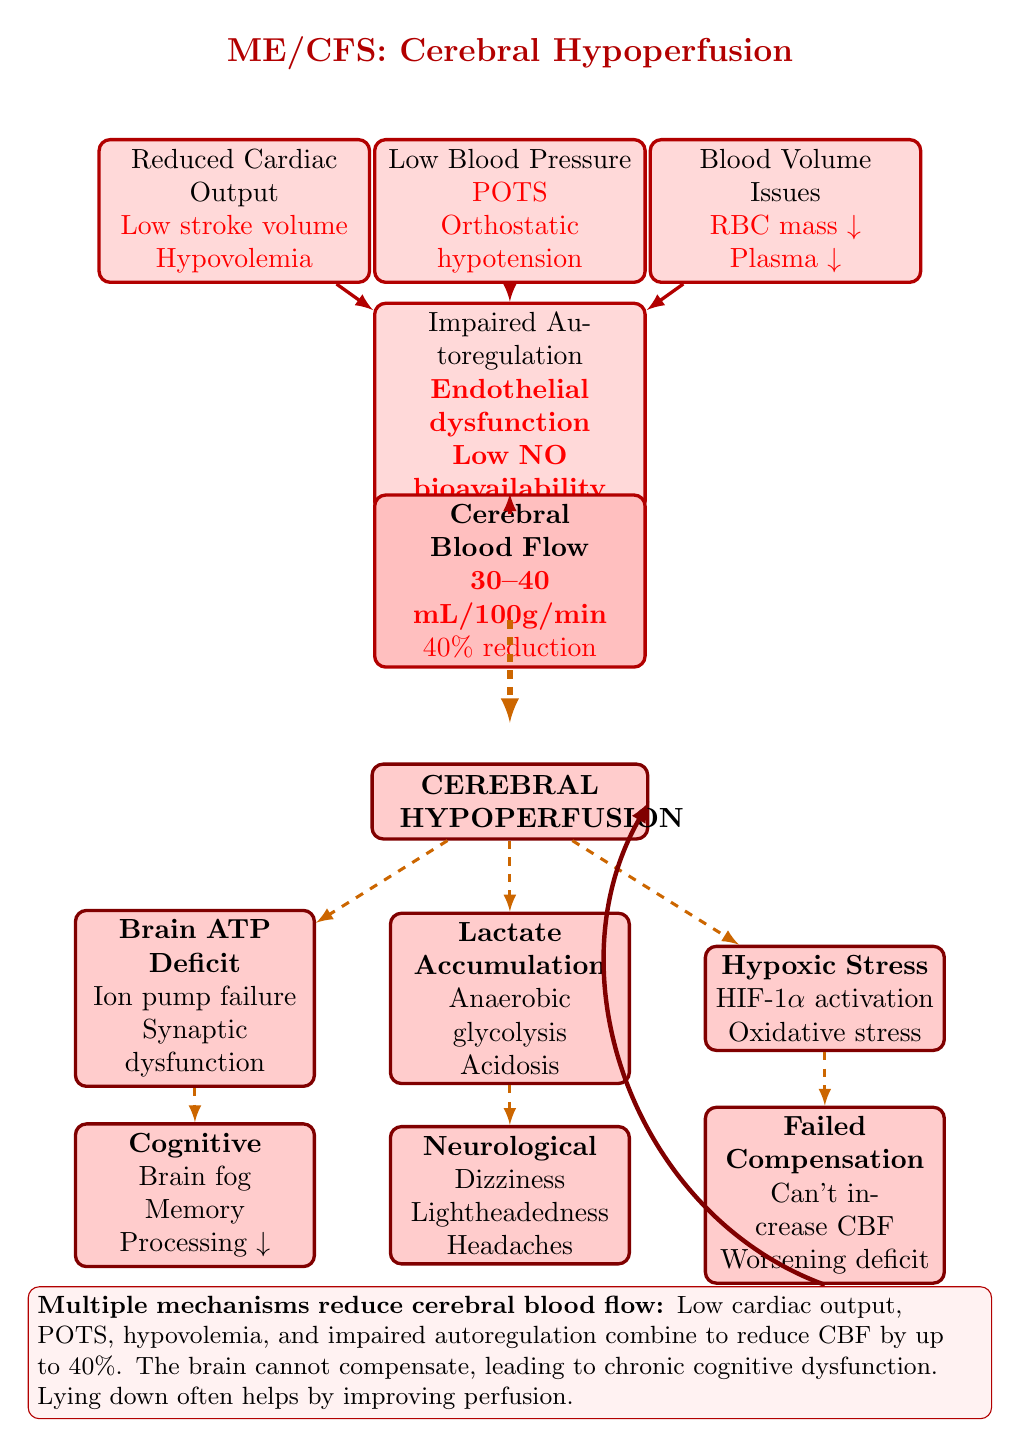
\begin{tikzpicture}[scale=1, every node/.style={scale=1},
    % Styles
    normal/.style={draw=green!70!black, fill=green!10, very thick, rounded corners, text width=3cm, align=center, minimum height=1cm},
    impaired/.style={draw=red!70!black, fill=red!15, very thick, rounded corners, text width=3.2cm, align=center, minimum height=1cm},
    severe/.style={draw=red!50!black, fill=red!25, ultra thick, rounded corners, text width=3.2cm, align=center, minimum height=1.1cm, drop shadow},
    pathological/.style={draw=red!50!black, fill=red!20, very thick, rounded corners, text width=2.8cm, align=center, minimum height=0.95cm},
    impaired-arrow/.style={-latex, very thick, red!70!black, line width=1.2pt},
    cascade-arrow/.style={-latex, thick, orange!80!black, dashed, line width=1.1pt},
    cycle-arrow/.style={-latex, ultra thick, red!50!black, line width=1.6pt},
    note/.style={font=\small\itshape, text width=2.4cm, align=left, red!60!black},
]

% Title
\node[font=\large\bfseries, red!70!black] at (0, 9) {ME/CFS: Cerebral Hypoperfusion};

% TOP: Impaired flow pathway
\begin{scope}[yshift=4.5cm]
    % Multiple contributors
    \node[impaired] (cardiac) at (-3.5, 2.5) {Reduced Cardiac\\Output\\{\color{red}Low stroke volume}\\{\color{red}Hypovolemia}};

    \node[impaired] (bp) at (0, 2.5) {Low Blood Pressure\\{\color{red}POTS}\\{\color{red}Orthostatic\\hypotension}};

    \node[impaired] (volume) at (3.5, 2.5) {Blood Volume\\Issues\\{\color{red}RBC mass $\downarrow$}\\{\color{red}Plasma $\downarrow$}};

    % Impaired autoregulation
    \node[impaired] (autoreg) at (0, 0) {Impaired Autoregulation\\{\color{red}\textbf{Endothelial dysfunction}}\\{\color{red}\textbf{Low NO bioavailability}}};
    \draw[impaired-arrow] (cardiac) -- (autoreg);
    \draw[impaired-arrow] (bp) -- (autoreg);
    \draw[impaired-arrow] (volume) -- (autoreg);

    % Reduced CBF
    \node[impaired, fill=red!25] (cbf) at (0, -2.2) {\textbf{Cerebral Blood Flow}\\{\color{red}\textbf{30--40 mL/100g/min}}\\{\color{red}40\% reduction}};
    \draw[impaired-arrow] (autoreg) -- (cbf);
\end{scope}

% BOTTOM: Cascade consequences
\begin{scope}[yshift=-3.5cm]
    % Central hypoperfusion
    \node[pathological, minimum width=3.5cm] (hypoperf) at (0, 3) {\textbf{CEREBRAL}\\  \textbf{HYPOPERFUSION}};

    % Three immediate consequences
    \node[pathological] (atp) at (-4, 0.5) {\textbf{Brain ATP}\\  \textbf{Deficit}\\Ion pump failure\\Synaptic dysfunction};

    \node[pathological] (lactate) at (0, 0.5) {\textbf{Lactate}\\  \textbf{Accumulation}\\Anaerobic glycolysis\\Acidosis};

    \node[pathological] (hypoxia) at (4, 0.5) {\textbf{Hypoxic Stress}\\HIF-1$\alpha$ activation\\Oxidative stress};

    \draw[cascade-arrow] (hypoperf) -- (atp);
    \draw[cascade-arrow] (hypoperf) -- (lactate);
    \draw[cascade-arrow] (hypoperf) -- (hypoxia);

    % Downstream symptoms
    \node[pathological] (cognitive) at (-4, -2) {\textbf{Cognitive}\\Brain fog\\Memory\\Processing $\downarrow$};

    \node[pathological] (neuro) at (0, -2) {\textbf{Neurological}\\Dizziness\\Lightheadedness\\Headaches};

    \node[pathological] (failed) at (4, -2) {\textbf{Failed}\\  \textbf{Compensation}\\Can't increase CBF\\Worsening deficit};

    \draw[cascade-arrow] (atp) -- (cognitive);
    \draw[cascade-arrow] (lactate) -- (neuro);
    \draw[cascade-arrow] (hypoxia) -- (failed);

    % Feedback loop
    \draw[cycle-arrow, bend left=50] (failed.south) to (hypoperf.east);
\end{scope}

% Arrow connecting top to bottom
\draw[cascade-arrow, line width=2pt] (0, 1.8) -- (0, 0.5);

% Key point box
\node[draw=red!70!black, fill=red!5, rounded corners, text width=12cm, align=left, font=\small] at (0, -7.5) {
\textbf{Multiple mechanisms reduce cerebral blood flow:} Low cardiac output, POTS, hypovolemia, and impaired autoregulation combine to reduce CBF by up to 40\%. The brain cannot compensate, leading to chronic cognitive dysfunction. Lying down often helps by improving perfusion.
};

\end{tikzpicture}
\caption{ME/CFS cerebral hypoperfusion cascade causing cognitive dysfunction.}
\label{fig:cerebral-hypoperfusion-mecfs}
\end{figure}


Figures~\ref{fig:cerebral-hypoperfusion-normal} and~\ref{fig:cerebral-hypoperfusion-mecfs} illustrate how multiple mechanisms reduce cerebral blood flow in ME/CFS (30--40 mL/100g/min vs.\ normal 50--60 mL/100g/min, a 40\% reduction).

\subsection{Reduced Regional Blood Flow}

Multiple neuroimaging modalities have demonstrated CBF reductions~\cite{vanCampen2020severity}:

\begin{itemize}
    \item \textbf{Global hypoperfusion}: 10--20\% reduction in total cerebral blood flow (measured by SPECT and Doppler ultrasound)
    \item \textbf{Regional deficits}: Particularly in frontal, temporal, and parietal regions
    \item \textbf{Brainstem hypoperfusion}: Potentially explaining autonomic dysfunction~\cite{Barnden2011brainstem}
    \item \textbf{Subcortical abnormalities}: Basal ganglia and thalamic hypoperfusion
\end{itemize}

Van Campen et al.~\cite{vanCampen2020severity} documented that 90\% of ME/CFS patients (n=429) showed abnormal CBF reduction (>13\%) during head-up tilt testing, with end-tilt CBF reduction of 26\% in ME/CFS patients versus only 7\% in controls (n=44). Importantly, this occurred even in the absence of hypotension or tachycardia, indicating intrinsic cerebrovascular dysfunction rather than solely cardiovascular causes.

\subsection{Correlation with Cognitive Symptoms}

CBF reductions correlate with specific cognitive deficits:

\begin{itemize}
    \item Frontal hypoperfusion → executive dysfunction, working memory impairment
    \item Temporal hypoperfusion → verbal memory deficits, language processing difficulties
    \item Parietal hypoperfusion → attention deficits, spatial processing impairment
    \item Global hypoperfusion → processing speed reduction, mental fatigue
\end{itemize}

\subsection{Mechanisms of Cerebral Hypoperfusion}

The cerebral hypoperfusion documented above likely results from multiple converging mechanisms:

\begin{itemize}
    \item \textbf{Reduced cardiac output}: Secondary to autonomic dysfunction (Section~\ref{sec:ans-pathophysiology}) and blood volume deficits~\cite{Streeten1998blood}
    \item \textbf{Impaired cerebral autoregulation}: Inability to maintain CBF across blood pressure changes~\cite{Barnden2011brainstem}
    \item \textbf{Endothelial dysfunction}: Reduced nitric oxide-mediated vasodilation
    \item \textbf{Increased cerebrovascular resistance}: Vasoconstriction or structural changes
    \item \textbf{Neurovascular uncoupling}: Failure of blood flow to match metabolic demand
\end{itemize}

The integration of autonomic dysfunction, reduced blood volume, and direct cerebrovascular pathology creates a multifactorial reduction in brain perfusion that correlates with cognitive symptom severity. This multifactorial integration is characteristic of ME/CFS pathophysiology and is discussed in the context of multi-system interactions in Chapter~\ref{ch:integrative-models}, Section~\ref{sec:synthesis}.

\subsection{Exacerbation with Exertion}

Importantly, cerebral perfusion abnormalities worsen following physical or cognitive exertion:

\begin{itemize}
    \item Further CBF reductions post-exercise
    \item Prolonged recovery of normal perfusion
    \item Correlation with post-exertional malaise severity
    \item Potential contribution to cognitive ``crashes'' following activity
\end{itemize}

\section{Auditory Processing Dysfunction and Tinnitus}
\label{sec:auditory-dysfunction}

Auditory symptoms represent an underrecognized but significant neurological manifestation of ME/CFS, with convergent evidence from functional, epidemiological, systematic, and anatomical studies establishing auditory dysfunction as a documented feature of the disease.

\subsection{Prevalence and Epidemiology}

\begin{achievement}[Tinnitus-ME/CFS Epidemiological Association]
\label{ach:schubert2021-tinnitus}
Schubert et al.~\cite{Schubert2021} provided the first large-scale epidemiological evidence linking ME/CFS to tinnitus in a population-based cohort of 124,609 individuals from the Dutch Lifelines study. ME/CFS patients demonstrated 1.57 times higher odds (OR 1.568, p<0.05) of experiencing constant tinnitus compared to healthy controls, identifying ME/CFS as a novel disease associate for tinnitus beyond traditional audiological causes such as noise exposure, age-related hearing loss, and cardiovascular disease.
\end{achievement}

This finding aligns with earlier cohort studies and patient surveys reporting tinnitus prevalence ranging from 48\% to 78\% in ME/CFS patients, substantially higher than the 10--15\% prevalence in the general population.

\begin{achievement}[Systematic Evidence for Auditory Dysfunction]
\label{ach:skare2024-ear}
A 2024 systematic review by Skare et al.~\cite{Skare2024} synthesized evidence from 172 articles (1990--2024) documenting ear abnormalities across ME/CFS, fibromyalgia, long-COVID syndrome, postural orthostatic tachycardia syndrome (PoTS), and related conditions. The review identified cochlear complaints---including tinnitus, hearing loss, and hyperacusis---as the most frequent auditory findings in ME/CFS. Four pathophysiological mechanisms were proposed: (1) viral effects on cochlear or central auditory structures, (2) vascular impairment reducing blood flow to the cochlea and brainstem, (3) autoimmune reactions targeting inner ear antigens, and (4) oxidative stress damaging cochlear hair cells and auditory neurons.
\end{achievement}

The systematic review recommended that all ME/CFS patients with audiological complaints receive ENT consultation and formal audiometry to assess the nature and severity of auditory dysfunction.

\subsection{Functional Auditory Processing Deficits}

Beyond subjective tinnitus complaints, objective evidence demonstrates specific auditory processing impairments in ME/CFS patients.

\begin{achievement}[Selective Auditory Processing Impairment]
\label{ach:johnson1996-auditory}
Johnson et al.~\cite{Johnson1996} demonstrated modality-specific cognitive impairment in a controlled comparison of 20 CFS patients, 20 multiple sclerosis (MS) patients, and 20 healthy controls. CFS patients showed differential impairment on auditory versus visual processing tasks, while MS patients showed equal impairment on both modalities. This pattern suggests specific dysfunction in central auditory pathways rather than general cognitive slowing, distinguishing the ME/CFS cognitive profile from the more global impairment observed in other neurological conditions.
\end{achievement}

Functional MRI studies have further documented that CFS patients utilize more extensive brain regions for auditory processing compared to controls, requiring greater neural recruitment and elevated source current to achieve equivalent performance. This suggests inefficient auditory processing requiring compensatory activation of additional neural networks.

\subsection{Neuroanatomical Substrate: Brainstem Dysfunction}

The functional auditory deficits and elevated tinnitus prevalence in ME/CFS are explained by documented structural and functional abnormalities in brainstem regions critical for auditory processing.

\begin{achievement}[Brainstem Structural Abnormalities]
\label{ach:nelson2021-brainstem}
Nelson et al.~\cite{Nelson2021} synthesized MRI evidence from 11 studies demonstrating structural and functional brainstem abnormalities in ME/CFS patients. The brainstem contains the primary central auditory pathway structures:

\begin{itemize}
    \item \textbf{Cochlear nucleus} (medulla) --- receives input from cochlear nerve; first central processing station
    \item \textbf{Superior olivary complex} (pons) --- sound localization via interaural time and intensity differences
    \item \textbf{Lateral lemniscus} --- ascending auditory pathway connecting lower and upper brainstem
    \item \textbf{Inferior colliculus} (midbrain) --- integration of ascending auditory information before thalamic relay
\end{itemize}

Dysfunction in these structures provides a neuroanatomical substrate explaining both the auditory processing deficits documented by Johnson et al.~\cite{Johnson1996} and the increased tinnitus prevalence observed by Schubert et al.~\cite{Schubert2021}.
\end{achievement}

Importantly, brainstem abnormalities in ME/CFS extend beyond auditory pathways to include autonomic control centers (see Section~\ref{sec:ans-pathophysiology}), arousal systems (locus coeruleus), and sensory integration regions. This explains the co-occurrence of auditory symptoms with autonomic dysfunction, sleep disturbances, and sensory hypersensitivity---all manifestations of brainstem pathology.

\subsection{Central vs. Peripheral Auditory Pathology}

\begin{observation}[Central vs. Peripheral Auditory Pathology]
\label{obs:central-auditory}
The convergence of functional deficits~\cite{Johnson1996}, population-level tinnitus prevalence~\cite{Schubert2021}, systematic evidence~\cite{Skare2024}, and brainstem MRI abnormalities~\cite{Nelson2021} suggests predominantly \textbf{central (brainstem)} rather than peripheral (cochlear) auditory pathology in ME/CFS. This distinction has important therapeutic implications: neurological approaches targeting brainstem dysfunction, cerebral perfusion, and neuroinflammation may be more effective than peripheral ENT interventions focused solely on the cochlea or middle ear.
\end{observation}

Evidence supporting central over peripheral pathology includes:

\begin{itemize}
    \item Auditory processing deficits may occur without peripheral hearing loss on audiometry
    \item Tinnitus severity often fluctuates with orthostatic stress and cerebral hypoperfusion
    \item Auditory symptoms co-occur with other brainstem-mediated dysfunction (autonomic, arousal, sensory)
    \item Hyperacusis (sound sensitivity) suggests central gain dysregulation rather than peripheral damage
    \item Auditory symptoms are part of broader post-exertional malaise rather than isolated ear pathology
\end{itemize}

\subsection{Proposed Mechanisms}

Based on the systematic review by Skare et al.~\cite{Skare2024} and integration with established ME/CFS pathophysiology, four mechanisms likely contribute to auditory dysfunction (this exemplifies the multi-mechanism pattern characteristic of ME/CFS symptoms, as discussed in Chapter~\ref{ch:integrative-models}):

\paragraph{Viral Effects.}
Direct viral damage to cochlear structures or central auditory pathways may occur during acute infection. This is particularly relevant for post-infectious ME/CFS onset, where viral neurotropism (e.g., EBV, HHV-6) could affect brainstem auditory nuclei. Acute onset of tinnitus following infection supports this mechanism.

\paragraph{Vascular Impairment.}
Reduced cerebral blood flow documented in ME/CFS (Section~\ref{sec:cerebral-blood-flow}) likely affects the highly vascularized cochlea and brainstem auditory centers. The stria vascularis in the cochlea maintains the ionic gradient essential for sound transduction and is metabolically active, making it vulnerable to hypoperfusion. Fluctuating tinnitus severity correlating with orthostatic stress supports vascular involvement.

\paragraph{Autoimmune Reactions.}
Antibodies targeting inner ear antigens (anti-cochlin, anti-HSP70) or auditory brainstem structures may produce autoimmune inner ear disease (AIED). This mechanism aligns with broader autoimmune theories of ME/CFS and suggests potential benefit from immunomodulatory treatment in select patients.

\paragraph{Oxidative Stress.}
Reactive oxygen species generated by mitochondrial dysfunction and neuroinflammation can damage cochlear hair cells and auditory neurons. The cochlea has high metabolic demands and limited antioxidant capacity, making it vulnerable to oxidative damage. This mechanism connects auditory dysfunction to the mitochondrial pathology documented in ME/CFS.

\subsection{Clinical Implications}

\subsubsection{Assessment Recommendations}

Based on the documented prevalence and clinical significance of auditory dysfunction:

\begin{enumerate}
    \item \textbf{Routine screening}: All ME/CFS patients should be screened for tinnitus, hearing loss, hyperacusis, and auditory processing difficulties
    \item \textbf{Formal audiometry}: Patients reporting auditory symptoms should receive comprehensive audiological evaluation
    \item \textbf{ENT consultation}: Rule out treatable peripheral causes (cerumen impaction, otosclerosis, Ménière's disease)
    \item \textbf{Central auditory testing}: Consider auditory brainstem response (ABR) testing to assess central pathways
    \item \textbf{Correlation with ME/CFS severity}: Document whether auditory symptoms fluctuate with overall disease activity, orthostatic stress, and post-exertional malaise
\end{enumerate}

\subsubsection{Treatment Considerations}

Given the proposed central pathology:

\begin{itemize}
    \item \textbf{Address underlying ME/CFS pathophysiology}: Optimize cerebral perfusion (salt/fluid loading for orthostatic intolerance), treat neuroinflammation, support mitochondrial function
    \item \textbf{Symptomatic management}: Sound therapy (white noise, tinnitus masking), cognitive-behavioral therapy for tinnitus distress (distinct from CBT as ME/CFS treatment)
    \item \textbf{Avoid ototoxic medications}: Many drugs can worsen tinnitus (aminoglycosides, loop diuretics, high-dose aspirin, certain chemotherapies)
    \item \textbf{Consider immunomodulation}: In patients with evidence of autoimmune component (autoantibodies, inflammatory markers)
    \item \textbf{Antioxidant support}: Alpha-lipoic acid, CoQ10, N-acetylcysteine (extrapolated from evidence in age-related hearing loss and noise-induced damage)
\end{itemize}

\begin{warning}[Tinnitus as PEM Symptom]
Many ME/CFS patients report that tinnitus intensity increases during post-exertional malaise or correlates with fatigue severity. This pattern suggests tinnitus may function as a real-time indicator of energy depletion or cerebral hypoperfusion. Patients should be educated to recognize worsening tinnitus as a potential warning sign to rest and avoid further exertion.
\end{warning}

\subsection{Research Gaps}

Despite the convergent evidence for auditory dysfunction in ME/CFS, significant gaps remain:

\begin{itemize}
    \item \textbf{Causality}: Cross-sectional designs cannot determine whether ME/CFS causes auditory dysfunction, auditory dysfunction contributes to ME/CFS symptoms, or a common mechanism produces both
    \item \textbf{Subtype correlation}: Unknown whether auditory symptoms predict specific ME/CFS subgroups or correlate with particular biomarkers
    \item \textbf{Treatment trials}: No randomized controlled trials of auditory-targeted interventions in ME/CFS populations
    \item \textbf{Mechanism validation}: The four proposed mechanisms (viral, vascular, autoimmune, oxidative) require experimental validation
    \item \textbf{Reversibility}: Unknown whether treating underlying ME/CFS pathophysiology can reverse auditory dysfunction
    \item \textbf{Longitudinal trajectory}: Natural history of auditory symptoms in ME/CFS not systematically documented
\end{itemize}

\begin{open_question}[Central Auditory Gain and Sensory Hypersensitivity]
Hyperacusis (sound sensitivity) in ME/CFS may reflect dysregulated central gain in auditory processing pathways. The brainstem and auditory cortex normally adjust sensitivity (gain) based on environmental demands and context. In ME/CFS, chronic neuroinflammation, altered neurotransmitter levels, or thalamic dysfunction may inappropriately increase central auditory gain, amplifying all sounds and making normal environmental noise intolerable. This would parallel central sensitization in pain pathways. Testing this hypothesis with objective measures of auditory gain (acoustic reflex thresholds, loudness discomfort levels, auditory brainstem response) could clarify mechanisms and guide treatment targeting central gain normalization rather than peripheral protection.
\end{open_question}

\section{Cognitive Dysfunction: Clinical Manifestations}
\label{sec:cognitive-clinical}

The neurological abnormalities described above manifest clinically as characteristic patterns of cognitive dysfunction, often described by patients as ``brain fog.''

\subsection{Domains of Impairment}

\subsubsection{Processing Speed}

Slowed information processing is perhaps the most consistent cognitive finding, manifesting as delayed reaction times, slower performance on timed tasks, reduced ability to keep up with rapid conversations, and difficulty with time-pressured activities.

\subsubsection{Attention and Concentration}

Attention and concentration deficits include difficulty sustaining attention, easy distractibility, impaired divided attention (multitasking), and reduced attentional capacity under stress.

\subsubsection{Memory}

Memory impairments encompass working memory deficits (holding information ``online''), impaired short-term memory encoding, word-finding difficulties, and variable long-term memory retrieval.

\begin{hypothesis}[Memory Triage Consequence]
\label{hyp:memory-triage-consequence}

Memory encoding is substantially more energy-expensive than memory retrieval, predicting that ME/CFS patients should show disproportionate encoding deficits relative to retrieval impairment---a pattern consistent with CNS energy triage.

\paragraph{Differential energy costs of memory operations.}
Hippocampal memory encoding requires long-term potentiation (LTP), involving NMDA receptor activation, calcium-dependent signaling cascades, new protein synthesis, and structural synaptic remodeling~\cite{Kandel2014memory}. These processes are metabolically demanding: encoding a new memory trace requires de novo gene expression, dendritic spine growth, and synaptic protein trafficking. Retrieval, by contrast, reactivates existing synaptic patterns through pattern completion in CA3 networks---a process that uses established circuits without requiring new protein synthesis or structural modification~\cite{Dudai2015consolidation}.

Quantitative estimates suggest that LTP-associated protein synthesis increases local energy consumption by 30--50\% above baseline in hippocampal neurons, whereas pattern completion during retrieval operates within normal metabolic parameters. Working memory maintenance in prefrontal cortex similarly requires sustained neuronal firing against inhibitory currents, creating continuous metabolic demand proportional to the number of items held in mind~\cite{Constantinidis2018working}.

\paragraph{Predicted pattern in ME/CFS.}
If CNS energy is limited, the brain should sacrifice high-cost encoding operations before low-cost retrieval operations---a ``memory triage.'' This predicts:

\begin{enumerate}
    \item \textbf{Encoding $>$ retrieval impairment}: Patients should show greater difficulty forming new memories than accessing old ones. Standardized testing should reveal disproportionate deficits on encoding-dependent tasks (learning new word lists, forming new associations) relative to recognition or cued recall of previously encoded material
    \item \textbf{Working memory $>$ long-term retrieval}: Sustained prefrontal firing for working memory maintenance is metabolically costly; retrieving consolidated long-term memories from distributed cortical stores is less so
    \item \textbf{Encoding degrades with exertion}: During PEM, when CNS energy deficits intensify, new memory formation should decline more steeply than the ability to recall previously consolidated information
    \item \textbf{Context-dependent encoding failure}: Encoding in metabolically demanding contexts (noisy environments, multitasking, social interaction) should fail preferentially, as these conditions compete for the limited energy budget
\end{enumerate}

\paragraph{Supporting evidence.}
The meta-analysis by Sebaiti et al.~\cite{Sebaiti2022cognitive} documents memory impairment in ME/CFS with moderate effect sizes ($g = -0.55$ to $-0.67$), but existing studies have not systematically separated encoding from retrieval. Clinical observation consistently reports that ME/CFS patients struggle more with forming new memories (``I can't take in new information'') than with accessing established knowledge (``I remember things from before I got sick''). Patients frequently describe intact recognition (``I know I've seen this before'') with impaired free recall of recently encountered material---precisely the pattern predicted by encoding-selective energy limitation.

\paragraph{Treatment implications.}
If encoding is selectively impaired by energy limitation, compensatory strategies should emphasize: (1)~reducing encoding load through external memory aids (notes, recordings, photographs) rather than relying on internal encoding; (2)~scheduling new learning during peak energy windows; (3)~using spaced repetition to distribute encoding costs across multiple low-demand sessions; (4)~leveraging recognition over recall (multiple-choice formats, visual cues) when possible.

\paragraph{Limitations.}
This hypothesis has certainty 0.55. The differential energy cost of encoding versus retrieval is well established in neuroscience, but the specific prediction of disproportionate encoding impairment in ME/CFS awaits formal testing with paradigms designed to isolate encoding from retrieval. Existing neuropsychological batteries typically conflate encoding and retrieval in composite ``memory'' scores. Confounds include attention deficits (which impair encoding indirectly), medication effects, and sleep disruption (which impairs memory consolidation independently of encoding).
\end{hypothesis}

\subsubsection{Executive Function}

Executive function deficits present as planning and organization difficulties, impaired cognitive flexibility, reduced problem-solving ability, and difficulty with complex decision-making.

\subsection{Social and Emotional Dysfunction}
\label{subsec:social-emotional-dysfunction}

While less frequently discussed in clinical literature, social and emotional impairments represent significant sources of disability in ME/CFS and are direct consequences of the neurometabolic dysfunction documented above.

\textbf{Note on evidence base:} The detailed phenomenology described in this section is based primarily on extensive clinical observation and patient reports rather than systematic empirical research. While the underlying neurobiological mechanisms (catecholamine depletion, prefrontal hypometabolism, TPJ dysfunction) are well-documented~\cite{walitt2024deep}, the specific social and emotional manifestations described below await formal validation through patient surveys, qualitative research, and prospective studies. This section should be considered a synthesis of clinical observation with established neuroscience, not yet a body of peer-reviewed ME/CFS-specific research on social disability.

\subsubsection{Social Interaction as Metabolically Demanding Activity}

Social interaction requires the simultaneous coordination of multiple high-energy cognitive and neurological processes:

\begin{itemize}
    \item \textbf{Language processing and production}: Real-time comprehension, response formulation, word retrieval, and articulation
    \item \textbf{Working memory load}: Tracking conversational context, remembering prior statements, maintaining coherent narrative threads
    \item \textbf{Executive function demands}: Monitoring social cues, adjusting behavior in real-time, inhibiting inappropriate responses
    \item \textbf{Sensory integration}: Simultaneous processing of facial expressions, vocal prosody, body language, and environmental context
    \item \textbf{Motor control for affect generation}: Voluntary and involuntary facial expressions, eye contact, postural adjustments, vocal modulation
    \item \textbf{Reward system engagement}: Dopamine-mediated reward processing that makes social interaction inherently reinforcing in healthy individuals
\end{itemize}

When ATP production is impaired and catecholamine levels are low (as documented in the NIH study~\cite{walitt2024deep}), these processes cannot be sustained. The brain experiences social demands as it would physical exertion beyond capacity: as painful, threatening, something to avoid.

\subsubsection{Clinical Presentation: Social Interaction as Painful Exertion}

Many ME/CFS patients report that social interaction feels actively \textit{painful} rather than merely tiring:

\begin{itemize}
    \item Subjective experience identical to being forced to perform physical exercise while exhausted
    \item Approach characterized by ``minimize the pain''---engage only as much as absolutely necessary
    \item Absence of enjoyment or reward, even in interactions that would previously have been pleasurable
    \item Duration often measured in minutes before exhaustion becomes overwhelming
    \item Post-social crashes (cognitive and physical PEM) lasting hours to days
\end{itemize}

This pattern may persist for decades and often predates formal ME/CFS diagnosis, suggesting it reflects fundamental metabolic limitations rather than secondary depression or psychological withdrawal.

\subsubsection{Flat Affect and Energy Conservation}

Generating and displaying emotional affect is metabolically expensive:

\begin{itemize}
    \item \textbf{Muscular activation}: Smiling, animated facial expressions, and expressive body language require continuous motor control
    \item \textbf{Neurochemical substrates}: Emotional expression requires adequate dopamine for motivation and reward signaling
    \item \textbf{Prefrontal-limbic coordination}: Generating contextually appropriate affect requires coordination between multiple brain regions
\end{itemize}

When energy is scarce, the brain prioritizes survival functions over social signaling. The result is observable flat affect---patients appear emotionally unexpressive, disengaged, or ``unhappy'' even when not experiencing negative emotion. This is \textbf{not} conscious suppression or masking; it reflects genuine inability to generate the energetic and neurochemical processes required for emotional expression.

\subsubsection{Interpersonal Consequences and Misattribution}

The combination of social withdrawal and flat affect creates predictable interpersonal difficulties:

\begin{itemize}
    \item \textbf{Misinterpretation as contempt or disinterest}: Observers lacking context for the patient's energy deficit often interpret flat affect and minimal engagement as disdain, superiority, or lack of care
    \item \textbf{Relationship damage}: Colleagues, friends, and family members feel rejected, judged, or dismissed when the actual issue is metabolic incapacity
    \item \textbf{Emotional contagion}: Others interacting with ME/CFS patients often become unhappy or uncomfortable themselves, unable to understand the patient's apparent lack of positive affect
    \item \textbf{Inability to explain}: The exhaustion that prevents social engagement also impairs the cognitive and communication capacity needed to explain the problem (``explaining why I'm too tired to talk requires energy to talk'')
    \item \textbf{Vicious cycle}: Negative reactions from others increase the stress and energy demand of social interaction, further reducing capacity
\end{itemize}

Patients are frequently blamed for ``attitude problems,'' ``not trying,'' or ``not caring'' when the actual issue is neurometabolic failure to generate expected social signals.

\subsubsection{The Communication Double-Bind}

ME/CFS patients face an impossible situation regarding social interaction:

\begin{enumerate}
    \item Employment and relationships require communication and social engagement
    \item Communication and social engagement are painfully exhausting and worsen symptoms
    \item Avoiding social interaction damages relationships and is misinterpreted as contempt
    \item Explaining the difficulty requires the very communication capacity that is depleted
    \item There is no winning strategy---only choices between different types of harm
\end{enumerate}

\subsubsection{Relationship Conflict as Insurmountable Barrier}

The energy deficit affecting social interaction becomes critically limiting when relationships encounter even minor conflict or tension:

\begin{itemize}
    \item \textbf{Conflict management requires peak cognitive resources}: Navigating disagreements, processing emotions, formulating diplomatic responses, regulating one's own reactions, and sustaining conversation through discomfort all require executive function, emotional regulation, and sustained attention---precisely the capacities most impaired in ME/CFS

    \item \textbf{Minor conflicts become insurmountable}: What healthy individuals would consider trivial relationship friction (scheduling disagreements, differing preferences, minor miscommunications) becomes \textit{impossibly difficult to manage} when cognitive and emotional resources are depleted

    \item \textbf{Relationship attrition}: Friendships require ongoing maintenance, occasional conflict resolution, and emotional investment. When any conflict---however minor---exceeds available energy, relationships deteriorate and are eventually abandoned

    \item \textbf{Selection for low-maintenance relationships only}: Only relationships requiring absolutely minimal effort, zero conflict, and no emotional complexity can be sustained. This severely restricts social connection to a vanishingly small subset of potential relationships

    \item \textbf{Inability to repair}: Even when patients recognize that a relationship is worth preserving, they lack the energy to engage in the repair conversations necessary to resolve issues. The relationship fails not from lack of desire but from metabolic inability to execute repair

    \item \textbf{Compounding isolation}: As relationships with any degree of complexity or occasional friction are abandoned due to inability to manage conflict, social networks contract to near-zero. Patients become profoundly isolated not from preference but from inability to meet the basic energy demands of relationship maintenance

    \item \textbf{Loss of deep connections}: The inability to engage seriously in friendship---to invest emotional energy, navigate normal ups and downs, work through misunderstandings---means that only the most superficial relationships can survive. Patients lose access to the deep, meaningful connections that require tolerance for occasional difficulty

    \item \textbf{Present but disengaged}: Even when patients are physically able to attend activities or gatherings, the constant underlying exhaustion limits how intensely they can engage with others. They are there in body but cannot fully participate emotionally or socially. This creates a perceptible distance that has no apparent reason---others sense the patient is ``holding back'' or ``not really there,'' but the actual cause (metabolic inability to engage more deeply) is invisible

    \item \textbf{Engagement intensity limited by energy, not desire}: The degree of warmth, enthusiasm, investment, and genuine connection patients can offer is capped by available energy, not by their feelings toward others. Friendships that would otherwise be close remain distant because the patient cannot sustain the energy for deeper engagement, creating unexplained coldness that damages the relationship despite the patient's genuine care

    \item \textbf{Inability to develop meaningful feelings}: The energy limitation affects not only the expression of feelings but the development of feelings themselves. Emotional attachment, fondness, care, and affection require sustained interaction, shared experiences, emotional investment, and cognitive processing to develop. When energy constraints prevent this sustained engagement, feelings toward others remain shallow or fail to develop beyond superficial acquaintance. Patients find themselves unable to develop the deep care and emotional connection that would normally arise in friendships, creating a profound sense of emotional emptiness and isolation even when physically surrounded by potential friends

    \item \textbf{Social interactions as potential threats}: The knowledge that any conflict or difficulty is insurmountable leads to a defensive posture where many interactions are experienced as \textit{opportunities to be aggressed}. Since patients lack the energy to manage disagreement, navigate misunderstanding, or repair relationship damage, any interaction carries the risk of creating a problem they cannot solve. This produces preventive behavior---emotional guardedness, avoidance of deeper topics, reluctance to express needs or preferences---that further impedes the ability to connect with others. Patients become hypervigilant for potential conflict and withdraw preemptively to avoid situations they cannot metabolically handle, creating a self-protective isolation that others perceive as coldness or lack of trust
\end{itemize}

\textbf{Clinical significance:} The inability to manage even minimally conflictual relationships represents a major, under-recognized source of social disability in ME/CFS. \textbf{This cannot be understated}: patients lose friendships, partnerships, and entire social networks not because relationships are unimportant to them, but because the cognitive and emotional energy required to navigate normal relationship dynamics exceeds available capacity.

The defensive stance toward social interaction---experiencing interactions as potential threats and adopting preventive behaviors---is not paranoia or social anxiety disorder. It is a rational response to genuine incapacity. When any disagreement or misunderstanding represents an insurmountable problem due to energy deficit, hypervigilance and preemptive withdrawal become adaptive survival strategies, though they further entrench isolation.

Critically, \textit{the feeling alone is sufficient to drive protective behavior}. Patients do not need to consciously analyze the risk or make deliberate decisions to withdraw---the subjective experience of interactions as threatening automatically triggers defensive responses. This emotional reality shapes behavior independent of objective threat assessment, making the social disability self-reinforcing: the feeling of vulnerability produces protective isolation, which prevents connection, which maintains isolation.

\subsubsection{Environmental Control as Survival Mechanism}

The energy deficit necessitates a level of environmental control that is incompatible with normal social spontaneity and fundamentally at odds with what others experience as ``the joy of life'':

\begin{itemize}
    \item \textbf{Need for high control}: Patients require predictability, structure, and control over their environment to prevent energy-depleting surprises. Unforeseen events, changes in plans, unexpected social demands, or environmental chaos each represent potential energy expenditures that may trigger crashes

    \item \textbf{Incompatibility with spontaneity}: What healthy individuals experience as joyful spontaneity---surprise visits, impromptu plans, playful chaos, unexpected adventures---registers for ME/CFS patients as threatening unpredictability requiring energy they do not have

    \item \textbf{Others' joy as patient's stress}: When others behave in ways they enjoy---being spontaneous, playful, or socially unpredictable---they create a more energetically demanding environment for patients. The very behaviors that make life feel vibrant and enjoyable for healthy people increase the metabolic burden and stress for patients beyond what they can afford to manage

    \item \textbf{Inability to ``let go''}: Patients cannot easily relax control over their environment because this control is \textit{almost vital} to avoid exhaustion and crashes. What appears as rigidity, controlling behavior, or inability to be spontaneous is actually a survival mechanism---without environmental control, energy expenditure becomes unpredictable and unmanageable

    \item \textbf{Social consequences}: Others perceive the need for control as rigidity, inflexibility, being ``no fun,'' or being controlling. Patients are seen as unable to enjoy life, overly cautious, or anxiety-driven when the actual issue is metabolic necessity

    \item \textbf{The paradox of joy}: Patients are often told to ``relax,'' ``let go,'' ``be spontaneous,'' or ``just have fun''---but these very behaviors require energy reserves they do not possess. The inability to engage in joyful spontaneity is not psychological resistance but physiological impossibility
\end{itemize}

\textbf{The fundamental incompatibility:} Normal social life thrives on a degree of unpredictability, spontaneity, and flexibility that ME/CFS patients cannot metabolically afford. The environmental control necessary for survival (avoiding crashes, managing energy) is experienced by others as joyless rigidity. Patients must choose between:

\begin{enumerate}
    \item Maintaining control to prevent crashes (perceived as controlling, rigid, unable to have fun)
    \item Allowing spontaneity to please others (risking energy depletion, crashes, worsening disability)
\end{enumerate}

There is no middle ground when energy reserves are this limited. The choice to maintain control is not preference or personality---it is metabolic necessity masquerading as behavioral rigidity.

\paragraph{The Energy Poverty Analogy.}
The psychological state of ME/CFS patients living with severe energy deficit is analogous to the lived experience of people in extreme financial poverty:

\begin{itemize}
    \item \textbf{Constant precariousness}: Just as very poor people live under constant financial stress knowing that any unforeseen expense---even an insignificant 20--50\euro\ debt---could trigger a cascade of catastrophic consequences (eviction, utility shutoff, inability to afford food or medical care), ME/CFS patients live under constant metabolic stress knowing that any unforeseen energy expenditure can trigger crashes that eliminate function for days, weeks, or permanently

    \item \textbf{Inability to absorb shocks}: People with financial reserves can absorb unexpected expenses without crisis. People with energy reserves can absorb unexpected demands without crashing. Those living at the edge---whether financial or metabolic---have no buffer. Every unexpected demand is a potential catastrophe

    \item \textbf{Hypervigilance as survival}: The poor must constantly monitor their finances, avoid any unnecessary spending, and maintain rigid control over their budget to prevent disaster. ME/CFS patients must constantly monitor their energy, avoid any unnecessary expenditure, and maintain rigid control over their environment to prevent crashes. Both behaviors appear as anxiety or rigidity to those with adequate resources but are rational responses to genuine scarcity

    \item \textbf{Incomprehension from the resourced}: People with financial security cannot understand why the poor seem so anxious about ``small'' expenses or why they cannot ``just relax'' about money. People with energy reserves cannot understand why ME/CFS patients seem so anxious about ``small'' demands or why they cannot ``just relax'' and be spontaneous. The invisible nature of the deficit makes the defensive behavior appear irrational

    \item \textbf{Poverty trap dynamics}: Financial poverty creates conditions that perpetuate poverty (stress impairs decision-making, lack of resources prevents investment in improvement). Energy poverty creates conditions that perpetuate energy deficit (stress depletes energy, lack of reserves prevents activities that might improve capacity). Both are self-reinforcing traps difficult to escape

    \item \textbf{Judgment and blame}: The poor are blamed for being ``too cautious,'' ``no fun,'' unable to enjoy life, overly anxious, or having a scarcity mindset. ME/CFS patients are blamed for being controlling, rigid, unable to be spontaneous, overly anxious, or having a fearful personality. In both cases, the behavior is adaptive to genuine scarcity, not a character flaw
\end{itemize}

\textbf{Clinical significance:} Understanding ME/CFS energy management through the lens of poverty economics helps clarify why patients exhibit behaviors that appear rigid or controlling to healthy observers. The ``energy poverty'' framework explains the hypervigilance, need for control, inability to tolerate unpredictability, and constant stress as rational adaptations to living at the metabolic edge. Just as telling someone in extreme financial poverty to ``stop worrying about money and have fun'' is tone-deaf and unhelpful, telling ME/CFS patients to ``relax,'' ``let go,'' or ``be spontaneous'' fundamentally misunderstands their metabolic reality.

Even when patients \textit{can} attend activities, the pervasive exhaustion creates an invisible barrier to genuine engagement. Others perceive this as emotional distance, lack of interest, or ``holding back''---but it reflects metabolic incapacity, not psychological withdrawal. The patient may desperately want to engage more warmly, more deeply, with more enthusiasm and investment, but the energy simply does not exist. This creates relationships that feel inexplicably cold or distant despite no apparent reason, as the actual limitation (energy deficit) is invisible to observers.

This pattern is distinct from social anxiety or avoidant personality disorder---patients often desperately \textit{want} connection but physiologically \textit{cannot} sustain the energy expenditure relationships require, particularly when any degree of conflict or complexity arises.

\subsubsection{Neurobiological Basis}

The social and emotional impairments described above are explained by the documented neurological abnormalities:

\begin{itemize}
    \item \textbf{Catecholamine depletion}: Low dopamine and norepinephrine impair both reward processing (making social interaction unrewarding) and the motivation to engage socially
    \item \textbf{Prefrontal hypometabolism}: Reduced energy availability in prefrontal regions impairs the executive functions required for social cognition
    \item \textbf{Effort-reward miscalculation}: TPJ dysfunction causes the brain to perceive social interaction as high-cost, low-reward activity
    \item \textbf{Cerebral hypoperfusion}: Reduced blood flow limits the brain's capacity to sustain the metabolic demands of complex social processing
    \item \textbf{ATP depletion}: Fundamental energy insufficiency makes any sustained cognitive activity painful
\end{itemize}

\subsubsection{Clinical Significance}

\begin{tcolorbox}[colback=blue!5!white,colframe=blue!75!black,title=Recognition and Validation]
Social withdrawal and flat affect in ME/CFS are \textbf{metabolic symptoms}, not personality traits, character flaws, or pure psychiatric conditions.

\textbf{For patients:} If social interaction feels painful, if you feel no enjoyment in activities that once brought pleasure, if others tell you that you seem ``unhappy'' or ``unengaged''---these are recognized manifestations of the neurometabolic dysfunction documented in ME/CFS research. This is not your fault. You are not antisocial, cold, or broken. Your brain lacks the energy and neurochemical substrates required for normal social and emotional functioning.

\textbf{For clinicians and caregivers:} Patients who appear disengaged, flat, or ``unmotivated'' for social interaction are not exhibiting ``behavioral problems.'' They are conserving severely limited energy reserves. Pressure to ``be more social'' or ``act happier'' is equivalent to demanding that someone with severe anemia run a marathon. The physiology does not support the demand.

\textbf{For researchers:} The social and emotional dysfunction in ME/CFS deserves systematic study alongside more commonly recognized cognitive domains. Validated instruments for assessing ``social exhaustion,'' ``affective energy expenditure,'' and ``interpersonal metabolic cost'' would help quantify this significant source of disability.
\end{tcolorbox}

\begin{warning}[Harmful Advice: The ``Power of Positive Thinking'']
Some clinicians, family members, friends, and caregivers, despite good intentions, offer advice to ME/CFS patients that is not only unhelpful but actively harmful and insulting:

\textbf{The harmful message:}
\begin{itemize}
    \item ``You need to be more optimistic''
    \item ``Believing you will get better will make you better''
    \item ``Your attitude is holding you back''
    \item ``The mind-body connection means positive thinking can heal you''
    \item ``You need to stop focusing on your symptoms''
\end{itemize}

\textbf{Why this is harmful:}

\begin{enumerate}
    \item \textbf{Blames the patient for their illness}: This framing implies that patients are sick because they are not trying hard enough to think positively, placing moral responsibility for a metabolic disease on the patient's psychological state

    \item \textbf{Contradicts objective evidence}: The 2024 NIH study documented measurable neurological abnormalities---low catecholamines, TPJ dysfunction, cerebral hypoperfusion, T-cell exhaustion. These are not created or maintained by ``negative thinking'' and cannot be resolved by ``optimism''

    \item \textbf{Ignores patient experience}: Decades of lived experience show that ME/CFS patients who maintain hope, who try every treatment, who remain optimistic, still worsen or remain severely ill. The disease trajectory is independent of psychological attitude

    \item \textbf{Dismissive and insulting}: Telling someone with documented metabolic dysfunction that their attitude is the problem is equivalent to telling a diabetic that believing their pancreas works will make it produce insulin. It dismisses the physiological reality of the disease

    \item \textbf{Adds psychological burden}: Patients already carry immense guilt and self-blame (``Why can't I do what I used to do? Why am I letting everyone down?''). Being told their illness persists because they are not optimistic \textit{enough} adds psychological torment to physical suffering

    \item \textbf{Prevents appropriate treatment}: When clinicians attribute symptoms to psychological factors, they fail to investigate and treat the underlying metabolic, immunological, and neurological dysfunction

    \item \textbf{Gaslighting}: This advice constitutes medical gaslighting---denying the patient's lived reality and documented physiological abnormalities in favor of a psychosomatic explanation that places blame on the patient
\end{enumerate}

\textbf{The reality:}
\begin{itemize}
    \item ME/CFS patients are not sick because they lack optimism
    \item Positive thinking does not reverse catecholamine depletion, mitochondrial dysfunction, or immune exhaustion
    \item Many patients maintain hope and optimism for \textit{decades} while their condition worsens---their attitude did not prevent deterioration
    \item The mind-body connection exists, but it does not mean that metabolic diseases can be thought away
    \item Encouraging appropriate pacing, realistic expectations, and acceptance of limitations is more therapeutic than false promises that optimism will cure metabolic dysfunction
\end{itemize}

\textbf{For clinicians:} If you find yourself telling ME/CFS patients to ``be more optimistic'' or attributing their symptoms to psychological factors, recognize that you are:
\begin{enumerate}
    \item Contradicting objective research evidence
    \item Causing psychological harm
    \item Failing to provide appropriate medical care
    \item Perpetuating the decades of medical gaslighting that has defined ME/CFS patient experience
\end{enumerate}

The appropriate clinical response is to acknowledge the physiological reality of the disease, validate the patient's experience, support symptom management and pacing, and avoid placing the burden of recovery on the patient's psychological state.
\end{warning}

\subsection{Fluctuation and Post-Exertional Cognitive Malaise}

A characteristic feature distinguishing ME/CFS cognitive dysfunction from other conditions is its marked fluctuation, including hour-to-hour and day-to-day variability, worsening with physical, cognitive, or emotional exertion, delayed deterioration (cognitive ``payback''), and improvement with rest that rarely returns to premorbid baseline.


\subsection{CNS Energy Crisis as Primary Event}
\label{sec:cns-energy-crisis}

The selective energy dysfunction hypothesis (Section~\ref{sec:selective-dysfunction}) proposes that neurological symptoms in ME/CFS reflect \emph{primary} CNS energy failure rather than downstream effects of systemic dysfunction. Several observations support this framing:

\begin{enumerate}
    \item \textbf{CNS-specific findings}: Neuroinflammation (45--199\% elevation in key regions~\cite{Nakatomi2014neuroinflammation}), catecholamine deficiency in CSF, and regional hypometabolism are documented in the CNS specifically, not as reflections of peripheral dysfunction

    \item \textbf{Preserved autonomous processes}: Hair growth, nail growth, and basic wound healing---processes that operate locally without CNS coordination---remain intact even in severe ME/CFS, arguing against global metabolic failure

    \item \textbf{Demand-response failure}: The pattern of preserved baseline function with impaired challenge response (91--100\% show abnormal CBF reduction during orthostatic challenge~\cite{Novak2022}) is consistent with a CNS coordination bottleneck rather than peripheral end-organ dysfunction

    \item \textbf{Cognitive triage hierarchy}: The observation that complex cognition and executive function (``brain fog'') are affected before motor coordination or sensory processing suggests an energy triage system that sacrifices ``luxury'' cognitive functions first

    \item \textbf{Astrocyte vulnerability}: The brain's unique metabolic architecture---with neurons depending on astrocytes for lactate via the ANLS (Section~\ref{sec:astrocyte-energy-gate})---may create CNS-specific vulnerability not present in peripheral tissues with direct glucose access~\cite{Pellerin1994,Magistretti2018}
\end{enumerate}

This perspective has treatment implications: interventions that bypass CNS coordination (e.g., direct-acting autonomic agents like midodrine) or that specifically target CNS metabolism may be more effective than peripheral mitochondrial support alone.

\subsection{CNS Energy Triage: A Hierarchical Model of Brain Fog}
\label{sec:cns-energy-triage-clinical}

\begin{speculation}[CNS Energy Triage Hypothesis]
\label{spec:cns-energy-triage}
The brain may operate a hardwired energy prioritization system during metabolic scarcity, explaining why ME/CFS cognitive dysfunction follows a characteristic pattern rather than producing uniform degradation across all domains.

\paragraph{Neuroscience of brain energy prioritization.}
The human brain comprises approximately 2\% of body mass yet consumes 20--25\% of resting metabolic energy, with goal-directed cognition requiring only an additional $\sim$5\% above resting homeostatic costs~\cite{Jamadar2025metabolic}. This tight energy budget means that even modest metabolic deficits---such as those produced by impaired astrocyte-neuron lactate shuttling (Section~\ref{sec:astrocyte-energy-gate})---could disproportionately affect the most energy-intensive neural processes.

Not all brain regions have equal metabolic demands. The prefrontal and frontoparietal association cortices, which support executive function, cognitive flexibility, and novel problem-solving, exhibit the highest \emph{relative metabolic cost}---defined as energy utilization exceeding baseline activity levels~\cite{Jamadar2025metabolic}. In contrast, brainstem nuclei governing vital functions (respiration, cardiovascular regulation, arousal) and primary sensory cortices operate with lower relative metabolic overhead, relying on phylogenetically older, more energy-efficient circuits.

\paragraph{Evidence from metabolic disruption models.}
Two natural experiments demonstrate hierarchical cognitive shutdown under energy scarcity:

\begin{enumerate}
    \item \textbf{Hypoglycemia:} Acute reduction in brain glucose supply impairs complex higher-order cognitive processes at higher glucose thresholds and to a greater extent than lower-level functions. Executive functions show large effect sizes ($d > 0.8$) during hypoglycemia~\cite{Graveling2013hypoglycemia}, consistent with the prefrontal cortex's elevated metabolic sensitivity.

    \item \textbf{Anesthesia:} General anesthetics produce a hierarchical disconnection pattern in which prefrontal and association cortices are affected first, while primary sensory processing and thalamocortical connectivity remain preserved. Mashour characterizes this as preferential failure of ``rich club'' network hubs with greater metabolic demands~\cite{Mashour2024anesthesia}---an ``airport in a snowstorm'' analogy where the most connected, most metabolically expensive nodes fail first.
\end{enumerate}

Furthermore, prolonged cognitive work causes glutamate accumulation specifically in the lateral prefrontal cortex, making further executive function activation progressively more metabolically costly~\cite{Wiehler2022glutamate}. This suggests a built-in mechanism by which the brain curtails its most expensive operations when metabolic capacity is strained.

\paragraph{Application to ME/CFS.}
We speculate that ME/CFS produces a chronic version of this triage state. If total available CNS energy is reduced---whether through astrocyte dysfunction, reduced cerebral blood flow, or neuroinflammation---the brain may engage the same prioritization hierarchy that normally activates only during acute metabolic crises. The proposed triage order, from most to least protected, would be:

\begin{enumerate}
    \item Brainstem vital functions (preserved even in severe ME/CFS)
    \item Basic sensory processing (usually intact)
    \item Language comprehension (impaired only in severe cases)
    \item Motor coordination (degraded in moderate-severe disease)
    \item Memory consolidation (commonly affected)
    \item Executive function and cognitive flexibility (affected early, often prominently)
\end{enumerate}

This maps to the formal energy triage hypothesis developed in Section~\ref{sec:selective-dysfunction} (specifically Hypothesis~\ref{hyp:energy-triage}), but here we emphasize the clinical neuroscience basis rather than the mathematical framework.

\paragraph{An important caveat from meta-analytic evidence.}
The largest meta-analysis of cognitive impairment in ME/CFS (33 studies, $n = 1{,}086$) reveals that the observed pattern is more nuanced than a simple ``executive function fails first'' model~\cite{Sebaiti2022cognitive}. Processing speed shows the largest impairment ($g = -0.82$), followed by sustained attention ($g = -0.75$), then memory domains ($g = -0.55$ to $-0.67$), with executive function showing a smaller effect ($g = 0.42$) and instrumental functions preserved. This is important: processing speed is \emph{more} impaired than executive function on standard neuropsychological measures.

This apparent discrepancy may be reconciled by recognizing that processing speed is a \emph{global} measure of neural efficiency degraded by any reduction in brain energy delivery, not a specific cognitive tier. It reflects the overall metabolic throughput of cortical circuits rather than a discrete cognitive function. Additionally, standardized tests of executive function (e.g., Trail Making Test Part B) involve relatively routinized operations that may not capture the full metabolic cost of genuinely novel, unstructured problem-solving. The energy triage model predicts that \emph{novel, complex, integrative} cognitive operations fail first---not necessarily the specific neuropsychological domain labeled ``executive function'' in test batteries.

\paragraph{Testable predictions.}
If the CNS energy triage model is correct, the following should hold:
\begin{itemize}
    \item Novel tasks are impaired more than practiced routines at matched difficulty
    \item Working memory (high-energy encoding) fails before recognition memory (lower-energy pattern completion), as formalized in Hypothesis~\ref{hyp:memory-triage}
    \item Cognitive hierarchy of impairment maps to regional metabolic demand on FDG-PET
    \item Severity progression follows the triage order: mild ME/CFS shows primarily executive/speed deficits; severe ME/CFS additionally shows language and motor involvement
    \item Interventions that bypass energy-expensive processing (routinization, external cognitive scaffolding) should preferentially improve function
\end{itemize}

\paragraph{Treatment implications.}
If the brain operates in chronic triage mode, the therapeutic strategy shifts from ``try harder'' to ``reduce the load'': (1)~\emph{routinize} daily activities to shift them from energy-expensive prefrontal control to energy-efficient basal ganglia automaticity; (2)~use external cognitive scaffolding (lists, alarms, decision templates) to offload executive demands; (3)~schedule cognitively demanding tasks during peak energy windows when triage thresholds are temporarily relaxed; (4)~explore metabolic interventions (ketone supplementation, cerebral blood flow optimization) that may expand the total energy budget and raise triage thresholds across all tiers.

\paragraph{Limitations.}
This hypothesis faces several challenges: (1)~the meta-analytic evidence does not cleanly support executive function as the most impaired domain~\cite{Sebaiti2022cognitive}; (2)~the triage hierarchy has not been directly tested in ME/CFS with tasks specifically designed to probe each tier; (3)~alternative explanations for the cognitive pattern exist, including neuroinflammation-mediated cytokine effects on specific circuits~\cite{Bansal2025cognitive}, tryptophan pathway diversion, and autonomic-mediated cerebral hypoperfusion; (4)~the model may oversimplify what is likely a multi-mechanism process. The triage framework should be understood as one contributing mechanism among several, not a complete explanation for ME/CFS cognitive dysfunction.
\end{speculation}

\section{Summary: An Integrated Neurological Model}
\label{sec:neuro-summary}

The evidence from the NIH deep phenotyping study and decades of prior research supports an integrated model of neurological dysfunction in ME/CFS~\cite{walitt2024deep}. An initiating trigger such as infection or other stressor disrupts central nervous system homeostasis. Microglial activation persists beyond acute illness, producing chronic low-grade neuroinflammation. Catecholamine and tryptophan pathway abnormalities develop, affecting dopamine, norepinephrine, and serotonin signaling (neurotransmitter dysregulation). The temporal-parietal junction and related regions fail to accurately process effort-related information (integrative brain dysfunction). Parasympathetic withdrawal and sympathetic dysregulation produce cardiovascular and multi-organ effects (autonomic dysfunction). Reduced cerebral blood flow limits brain metabolic capacity (cerebrovascular compromise). Finally, fatigue, cognitive dysfunction, orthostatic intolerance, and other symptoms emerge from these converging abnormalities as the clinical manifestations.

This model explains why ME/CFS patients experience fatigue fundamentally different from normal tiredness: the brain's basic mechanisms for perceiving, estimating, and responding to effort are dysfunctional. Treatment approaches targeting these specific neurological abnormalities may prove more effective than those addressing peripheral fatigue or deconditioning.

\begin{warning}[Stimulant Contraindication]
Stimulants (amphetamines, methylphenidate, modafinil) are generally \textbf{contraindicated} in ME/CFS despite their effectiveness in other fatigue conditions. While they may temporarily mask fatigue by artificially boosting alertness and motivation, they do not address the underlying energy deficit and may enable activity levels that exceed the patient's true physiological capacity. This can precipitate post-exertional malaise (PEM) and potentially cause permanent deterioration. The neurological model presented here explains why: stimulants affect perceived effort and motivation (downstream of the TPJ dysfunction) without correcting the fundamental mismatch between the brain's effort calculations and actual metabolic capacity. Patients may feel capable of activity that their bodies cannot sustain, leading to crashes. This differs fundamentally from stimulant use in conditions like ADHD or narcolepsy, where the underlying metabolic machinery is intact.
\end{warning}

\chapter{Endocrine and Metabolic Dysfunction}
\label{ch:endocrine}

\section{Hypothalamic-Pituitary-Adrenal (HPA) Axis}
\label{sec:hpa-axis}

% Insert Figure: Normal HPA Axis Function
% Figure: Normal HPA Axis Function
% Appropriate stress response with negative feedback control

\begin{figure}[htbp]
\centering
\begin{tikzpicture}[
    node distance=2.5cm,  % Global minimum vertical spacing
    % Styles
    process/.style={draw=green!70!black, fill=green!10, very thick, rounded corners, text width=4.5cm, align=center, minimum height=1.2cm},
    adaptive/.style={draw=green!70!black, fill=green!20, very thick, rounded corners, text width=4.5cm, align=center, minimum height=1.2cm},
    output/.style={draw=green!50!black, fill=green!30, ultra thick, rounded corners, text width=4.5cm, align=center, minimum height=1.3cm, drop shadow},
    arrow/.style={-latex, very thick, green!70!black, line width=1.2pt},
    feedback/.style={-latex, thick, blue!70!black, dashed, line width=1.1pt},
    note/.style={font=\small\itshape, text width=3.5cm, align=left, green!40!black},
]

% Title
\node[font=\large\bfseries, green!70!black] (title) at (0, 0) {Normal HPA Axis Function};

% Stressor
\node[process, below=3cm of title] (stressor) {\textbf{Stressor}\\[2pt] Physical or psychological};

% Hypothalamus
\node[process, below=of stressor] (hypothalamus) {\textbf{Hypothalamus}\\[2pt] CRH release};
\draw[arrow] (stressor) -- (hypothalamus);

% Pituitary
\node[adaptive, below=of hypothalamus] (pituitary) {\textbf{Pituitary}\\[2pt] ACTH release};
\draw[arrow] (hypothalamus) -- (pituitary);

% Adrenal
\node[adaptive, below=of pituitary] (adrenal) {\textbf{Adrenal Cortex}\\[2pt] Cortisol release};
\draw[arrow] (pituitary) -- (adrenal);
\node[note, left=1.5cm of adrenal, anchor=east] {
    \textbullet~Cortisol rhythm:\\~~~High AM\\~~~Low PM
};

% Cortisol effects
\node[adaptive, below=of adrenal] (cortisol) {\textbf{Cortisol Effects}\\[2pt] Mobilize energy\\Anti-inflammatory};
\draw[arrow] (adrenal) -- (cortisol);

% Negative feedback (right side)
\node[process, text width=3.8cm, right=5.5cm of pituitary] (feedback-box) {\textbf{Negative Feedback}\\[2pt] Cortisol inhibits\\CRH \& ACTH};
\draw[feedback, bend left=25] (cortisol.east) to (feedback-box.south);
\draw[feedback] (feedback-box) -- (hypothalamus);
\draw[feedback] (feedback-box) -- (pituitary);

% Recovery
\node[output, below=of cortisol] (recovery) {\textbf{STRESS RESOLUTION}\\[3pt] \textit{Return to baseline}\\[2pt] Homeostasis restored};
\draw[arrow] (cortisol) -- (recovery);

% Key point box
\node[draw=green!70!black, fill=green!5, rounded corners, text width=10cm, align=left, font=\small, inner sep=8pt, below=2.5cm of recovery] {
\textbf{Key characteristics:}\\[4pt]
\textbullet~Stressor activates hypothalamus $\rightarrow$ pituitary $\rightarrow$ adrenal cascade\\
\textbullet~Cortisol mobilizes energy and suppresses inflammation\\
\textbullet~Negative feedback prevents over-activation\\
\textbullet~System returns to baseline after stress resolves
};

\end{tikzpicture}
\caption{Normal HPA axis stress response with negative feedback control.}
\label{fig:hpa-axis-normal}
\end{figure}


% Insert Figure: ME/CFS HPA Axis Dysregulation
% Figure: HPA Axis Dysregulation in ME/CFS
% Blunted response, excessive feedback, systemic consequences

\begin{figure}[htbp]
\centering
\begin{tikzpicture}[scale=0.60, every node/.style={scale=0.60},
    % Styles
    normal/.style={draw=green!70!black, fill=green!10, very thick, rounded corners, text width=2.8cm, align=center, minimum height=0.85cm},
    impaired/.style={draw=red!70!black, fill=red!10, very thick, rounded corners, text width=2.8cm, align=center, minimum height=0.85cm},
    pathological/.style={draw=red!50!black, fill=red!20, very thick, rounded corners, text width=2.5cm, align=center, minimum height=0.85cm},
    impaired-arrow/.style={-latex, very thick, red!70!black},
    feedback/.style={-latex, thick, red!70!black, dashed},
    cascade-arrow/.style={-latex, thick, orange!80!black, dashed},
    note/.style={font=\scriptsize\itshape, text width=2.2cm, align=center},
]

% Title
\node[font=\large\bfseries, red!70!black] at (0, 9.5) {ME/CFS: HPA Axis Dysregulation};

% LEFT SIDE: Impaired pathway
\begin{scope}[xshift=-4.5cm]
    % Stressor
    \node[normal] (stressor) at (0, 7.5) {Stressor};

    % Hypothalamus - blunted
    \node[impaired] (hypothalamus) at (0, 5.5) {Hypothalamus\\{\color{red}\textbf{Blunted CRH}}\\{\color{red}Hypersensitive feedback}};
    \draw[impaired-arrow] (stressor) -- (hypothalamus);

    % Pituitary - impaired
    \node[impaired] (pituitary) at (0, 3.3) {Pituitary\\{\color{red}\textbf{Low ACTH}}\\{\color{red}Reduced reserve}};
    \draw[impaired-arrow] (hypothalamus) -- (pituitary);

    % Adrenal - atrophy
    \node[impaired] (adrenal) at (0, 1.1) {Adrenal Cortex\\{\color{red}\textbf{Atrophy/exhaustion}}\\{\color{red}Low output}};
    \draw[impaired-arrow] (pituitary) -- (adrenal);
    \node[note, left=0.2cm of adrenal, text=red!70!black] {Flattened\\rhythm:\\low all day};

    % Low cortisol
    \node[impaired, fill=red!25] (cortisol) at (0, -1.3) {\textbf{Low Cortisol}\\{\color{red}Can't mobilize energy}\\{\color{red}Can't suppress inflammation}};
    \draw[impaired-arrow] (adrenal) -- (cortisol);

    % Excessive feedback
    \node[impaired, text width=2.5cm] (feedback-box) at (3.5, 3.3) {\textbf{Excessive}\\  \textbf{Feedback}\\Over-suppression};
    \draw[feedback, bend left=20] (cortisol.east) to (feedback-box.south);
    \draw[feedback] (feedback-box) -- (hypothalamus);
    \draw[feedback] (feedback-box) -- (pituitary);

    % No recovery
    \node[impaired] (no-recovery) at (0, -3.5) {No Resolution\\{\color{red}Persistent dysfunction}};
    \draw[impaired-arrow] (cortisol) -- (no-recovery);
\end{scope}

% RIGHT SIDE: System failures
\begin{scope}[xshift=4.5cm]
    % Central dysfunction
    \node[pathological, minimum width=3.2cm] (hpa) at (0, 5) {\textbf{HPA AXIS}\\  \textbf{DYSFUNCTION}};

    % Six consequences in 2x3 grid
    \node[pathological] (stress) at (-2, 2.5) {\textbf{Stress}\\  \textbf{Intolerance}\\Can't cope\\Crashes};

    \node[pathological] (inflam) at (2, 2.5) {\textbf{Inflammation}\\  \textbf{Unchecked}\\No cortisol brake\\Cytokines high};

    \node[pathological] (metabolic) at (-2, 0) {\textbf{Metabolic}\\Hypoglycemia\\Poor energy\\mobilization};

    \node[pathological] (autonomic) at (2, 0) {\textbf{Autonomic}\\Orthostatic\\intolerance\\Low volume};

    \node[pathological] (mood) at (-2, -2.5) {\textbf{Mood}\\Depression\\Anxiety\\Brain fog};

    \node[pathological] (immune) at (2, -2.5) {\textbf{Immune}\\Th1/Th2\\imbalance\\Autoimmunity};

    % Cascade arrows
    \draw[cascade-arrow] (hpa) -- (stress);
    \draw[cascade-arrow] (hpa) -- (inflam);
    \draw[cascade-arrow] (hpa) -- (metabolic);
    \draw[cascade-arrow] (hpa) -- (autonomic);
    \draw[cascade-arrow] (hpa) -- (mood);
    \draw[cascade-arrow] (hpa) -- (immune);

    % Feedback from inflammation
    \draw[cascade-arrow, bend left=30, line width=1.5pt] (inflam.north) to (hpa.east);
    \node[font=\scriptsize, red!50!black, text width=1.5cm, align=center] at (3.5, 4) {Inflammation\\worsens HPA};
\end{scope}

% Key point box
\node[draw=red!70!black, fill=red!5, rounded corners, text width=12cm, align=left, font=\small] at (0, -6.5) {
\textbf{Blunted stress response:} Hypersensitive negative feedback over-suppresses the HPA axis. Low cortisol means inability to mobilize energy for stress, unchecked inflammation, metabolic instability, autonomic dysfunction, and mood problems. Inflammation feeds back to worsen HPA function.
};

\end{tikzpicture}
\caption{ME/CFS HPA axis dysregulation with blunted response and systemic consequences.}
\label{fig:hpa-axis-mecfs}
\end{figure}


Figures~\ref{fig:hpa-axis-normal} and~\ref{fig:hpa-axis-mecfs} illustrate HPA axis dysfunction in ME/CFS: blunted CRH release with hypersensitive feedback, low ACTH response, and flattened cortisol rhythm. This causes stress intolerance, unchecked inflammation, metabolic problems, autonomic dysfunction, and mood/cognitive issues.

\subsection{HPA Axis Abnormalities}
% Cortisol dysregulation
% ACTH levels
% CRH abnormalities
% Diurnal rhythm disruption

\subsection{Mechanisms of HPA Dysfunction}
% Central sensitivity changes
% Receptor alterations
% Feedback loop impairment

\subsection{Clinical Consequences}
% Stress response abnormalities
% Immune system effects
% Energy metabolism impact

\section{Thyroid Function}
\label{sec:thyroid}

% Thyroid hormone levels
% Tissue resistance
% Reverse T3
% Overlap with thyroid disorders

\section{Sex Hormones}
\label{sec:sex-hormones}

% Estrogen and progesterone
% Testosterone
% Menstrual cycle effects
% Gender differences in ME/CFS

\section{Growth Hormone and IGF-1}
\label{sec:growth-hormone}

% Deficiencies reported
% Effects on muscle and metabolism
% Treatment trials

\section{Insulin and Glucose Metabolism}
\label{sec:insulin-glucose}

% Insulin resistance patterns
% Glucose utilization impairments
% Hypoglycemia
% Connection to energy deficits

\section{Melatonin and Circadian Rhythms}
\label{sec:circadian}

% Circadian rhythm disruption
% Melatonin production
% Sleep-wake cycle abnormalities
% Clock gene expression

% FILE: Cardiovascular mechanisms — POTS, orthostatic intolerance, cardiac output, blood flow dysregulation, autonomic nervous system
\chapter{Cardiovascular Dysfunction}
\label{ch:cardiovascular}

Cardiovascular abnormalities are pervasive in ME/CFS and contribute substantially to disability, particularly through exercise intolerance and orthostatic symptoms. The 2024 NIH deep phenotyping study by Walitt et al.\ provided rigorous documentation of cardiopulmonary exercise testing abnormalities, including reduced peak oxygen consumption and chronotropic incompetence, establishing objective physiological correlates of the subjective exercise intolerance reported by patients~\cite{walitt2024deep}.

\section{Cardiac Function}
\label{sec:cardiac-function}

\subsection{Exercise Testing Abnormalities}
\label{sec:exercise-testing}

Cardiopulmonary exercise testing (CPET) provides objective measurement of integrated cardiovascular, pulmonary, and metabolic function during physical exertion. CPET findings in ME/CFS represent some of the most reproducible objective abnormalities documented in the illness.

\subsubsection{Cardiopulmonary Exercise Testing (CPET) Methodology}

CPET involves graded exercise (typically on a cycle ergometer or treadmill) with continuous measurement of oxygen consumption (VO$_2$, the volume of oxygen extracted from inspired air per unit time), carbon dioxide production (VCO$_2$, the volume of CO$_2$ expired), and their ratio expressed as the respiratory exchange ratio (RER = VCO$_2$/VO$_2$), which indicates fuel substrate utilization. Simultaneously, the system records minute ventilation (VE, total air volume breathed per minute), heart rate via continuous electrocardiographic monitoring, periodic blood pressure measurements, and work rate (power output in watts or treadmill speed and grade).

Testing continues until volitional exhaustion or limiting symptoms. Criteria for maximal effort include an RER exceeding 1.10, achievement of age-predicted maximal heart rate, or a plateau in VO$_2$ despite increasing work rate.

\subsubsection{Key NIH Deep Phenotyping CPET Findings}

The Walitt et al.\ study documented several critical cardiopulmonary abnormalities in PI-ME/CFS patients~\cite{walitt2024deep}:

\paragraph{Reduced Peak Oxygen Consumption (VO$_2$peak)}
Peak VO$_2$ represents maximal aerobic capacity and integrates cardiac output, oxygen delivery, and peripheral oxygen extraction. PI-ME/CFS patients demonstrated significantly reduced VO$_2$peak compared to matched healthy controls~\cite{walitt2024deep}. This reduction indicates impaired aerobic capacity beyond what deconditioning alone would predict; ME/CFS patients showed greater deficits than sedentary controls matched for activity level, with reductions typically ranging from 15--30\% below predicted values~\cite{keller2024cpet,lim2020cpet}. More severely affected patients show greater reductions. The finding correlates with functional limitation and disability, providing objective confirmation of patient-reported exercise intolerance.

\paragraph{Chronotropic Incompetence}
Chronotropic incompetence refers to an inadequate heart rate response to exercise~\cite{walitt2024deep}:

\begin{itemize}
    \item ME/CFS patients fail to achieve age-predicted maximal heart rate
    \item Heart rate rise is blunted relative to work rate increases
    \item Chronotropic index (proportion of heart rate reserve used) is reduced
\end{itemize}

Chronotropic incompetence limits cardiac output augmentation during exercise, as cardiac output = heart rate $\times$ stroke volume. Without adequate heart rate increase, oxygen delivery to exercising muscles is compromised.

\paragraph{Mechanisms of Chronotropic Incompetence}
Several mechanisms have been proposed; their relative contributions in ME/CFS remain under investigation:

\begin{enumerate}
    \item \textbf{Parasympathetic excess}: Sustained vagal tone preventing heart rate acceleration---supported by HRV findings showing altered autonomic balance~\cite{Newton2007autonomicDysfunction}
    \item \textbf{Sympathetic dysfunction}: Impaired catecholamine release or receptor sensitivity
    \item \textbf{Sinoatrial node dysfunction}: Intrinsic pacemaker abnormality (hypothesized but not directly demonstrated in ME/CFS)
    \item \textbf{G-protein-coupled receptor (GPCR) autoantibodies}: A growing body of evidence implicates autoantibodies targeting G-protein-coupled receptors in ME/CFS cardiovascular dysfunction. Loebel et al.\ first documented elevated autoantibodies against beta-adrenergic ($\beta_1$, $\beta_2$) and muscarinic cholinergic (M3, M4) receptors in ME/CFS patients~\cite{Loebel2016}, findings subsequently validated in Swedish cohorts including cerebrospinal fluid samples~\cite{Bynke2020}.

    The cardiovascular effects of these autoantibodies are multifaceted. Beta-adrenergic receptor autoantibodies may exert either agonistic effects (causing inappropriate receptor activation) or antagonistic effects (blocking normal catecholamine signaling), depending on the specific antibody epitope and receptor subtype. Muscarinic receptor autoantibodies similarly can enhance or impair parasympathetic signaling to the heart and vasculature. This bidirectional potential explains why the same class of autoantibodies might produce different phenotypes across patients.

    Levels of vasoregulative GPCR autoantibodies correlate with symptom severity, autonomic dysfunction, and disability in ME/CFS~\cite{Sotzny2021}. The correlation with autonomic measures supports a direct pathophysiological role rather than an epiphenomenon of chronic illness. Beta-2 adrenergic receptor autoantibodies appear particularly relevant to cardiovascular symptoms, with immunoadsorption targeting these antibodies showing preliminary efficacy in post-COVID ME/CFS~\cite{Stein2024immunoadsorption}. BC007, a DNA aptamer that neutralizes GPCR autoantibodies, has shown promise in case reports for improving fatigue and microcirculatory function~\cite{Hohberger2021bc007}.
    \item \textbf{Central nervous system dysfunction}: Impaired autonomic outflow from brainstem centers
    \item \textbf{Gut-mediated vagal impairment (hypothesized)}: Butyrate enhances enterochromaffin cell serotonin production~\cite{Barton2025}, and enterochromaffin serotonin activates vagal afferents via 5-HT$_3$ receptors~\cite{Barton2023,Kaelberer2018}. Since ME/CFS patients show butyrate deficiency, reduced enterochromaffin serotonin could impair vagal afferent signaling, potentially weakening efferent vagal tone to the heart. No direct evidence yet links this pathway to cardiac chronotropy in ME/CFS. See Section~\ref{sec:gut-brain} of Chapter~\ref{ch:gut-microbiome} for the full evidence chain
\end{enumerate}

The finding of chronotropic incompetence, combined with reduced HRV and abnormal baroreflex sensitivity~\cite{Newton2007autonomicDysfunction}, indicates autonomic dysfunction affecting cardiac pacing, though the primary site of dysfunction (central vs.\ peripheral) remains debated.

\subsubsection{Two-Day CPET Protocol}

A particularly informative methodology involves repeat CPET on consecutive days:

\paragraph{Rationale}
Single CPET testing may not capture the distinctive post-exertional deterioration characteristic of ME/CFS. Two-day protocols assess recovery capacity and reproducibility of maximal effort.

\paragraph{Findings in ME/CFS}
\begin{itemize}
    \item \textbf{Day 1}: Reduced but measurable aerobic capacity
    \item \textbf{Day 2}: Further significant reductions in VO$_2$peak, anaerobic threshold, and work capacity
    \item \textbf{Healthy controls}: Reproduce or slightly improve Day 1 performance
    \item \textbf{Magnitude}: ME/CFS patients show 10--25\% decline on Day 2~\cite{keller2024cpet,lim2020cpet}
\end{itemize}

This failure to reproduce exercise capacity distinguishes ME/CFS from other fatiguing conditions and reflects the pathognomonic post-exertional malaise~\cite{Lim2020}. A meta-analysis of two-day CPET studies confirmed significant reductions in work capacity and oxygen consumption on Day 2, supporting this protocol as an objective marker of PEM~\cite{lim2020cpet}.

\paragraph{Mechanisms of Day 2 Decline}
\begin{itemize}
    \item Delayed recovery of metabolic substrates
    \item Persistent inflammatory activation
    \item Autonomic dysfunction exacerbation
    \item Mitochondrial damage from oxidative stress
    \item Central nervous system effects (increased perceived exertion)
\end{itemize}

\subsubsection{Anaerobic Threshold}
\label{sec:anaerobic-threshold}

The anaerobic threshold (AT, also called ventilatory threshold or lactate threshold) represents the exercise intensity at which anaerobic metabolism begins to supplement aerobic energy production:

\begin{itemize}
    \item \textbf{Reduced AT in ME/CFS}: Occurs at lower work rates and VO$_2$ levels
    \item \textbf{Early lactate accumulation}: Muscles rely on anaerobic glycolysis sooner
    \item \textbf{Implications}: Limited sustainable activity before symptom exacerbation
    \item \textbf{Mechanism}: Reflects impaired oxygen delivery, mitochondrial dysfunction, or both
\end{itemize}

The reduced AT has practical implications: patients exceed their aerobic capacity during activities that healthy individuals perform entirely aerobically, leading to metabolic stress and symptom generation.

\subsubsection{Ventilatory Efficiency}
\label{sec:ventilatory-efficiency}

Ventilatory efficiency describes how effectively ventilation eliminates CO$_2$, typically expressed as the VE/VCO$_2$ slope:

\begin{itemize}
    \item \textbf{Increased VE/VCO$_2$ slope}: More ventilation required per unit CO$_2$ eliminated
    \item \textbf{Causes}: Ventilation-perfusion mismatch, increased dead space, hyperventilation
    \item \textbf{Consequences}: Dyspnea at lower work rates, earlier exercise termination
    \item \textbf{ME/CFS findings}: Variable; some patients show ventilatory inefficiency
\end{itemize}

\subsection{Cardiac Output and Stroke Volume}
\label{sec:cardiac-output}

Cardiac output (CO) determines oxygen delivery capacity and is the product of heart rate and stroke volume.

\subsubsection{Preload Failure Hypothesis}

Multiple lines of evidence support inadequate cardiac preload (ventricular filling) as a contributor to ME/CFS cardiovascular dysfunction:

\begin{itemize}
    \item \textbf{Reduced end-diastolic volume}: Less blood fills the ventricles during diastole
    \item \textbf{Decreased stroke volume}: By Frank-Starling mechanism, reduced preload produces smaller stroke volume
    \item \textbf{Compensatory tachycardia at rest}: Heart rate increases to maintain resting cardiac output; however, during exercise, chronotropic incompetence prevents further adequate heart rate augmentation, creating a ceiling effect
    \item \textbf{Exercise limitation}: The combination of low stroke volume and inadequate heart rate response severely limits cardiac output augmentation during exertion
\end{itemize}

\paragraph{Evidence for Preload Failure}
\begin{itemize}
    \item Echocardiographic studies showing reduced left ventricular end-diastolic volume
    \item Invasive hemodynamic measurements demonstrating low filling pressures
    \item Response to volume expansion (saline infusion) improving symptoms
    \item Correlation with blood volume measurements
\end{itemize}

\paragraph{Supine Hemodynamic Abnormalities}
While cardiovascular dysfunction in ME/CFS is most apparent during orthostatic stress, some patients demonstrate abnormalities even at rest in the supine position. Newton et al.\ documented reduced cardiac volumes on cardiac MRI that correlated with blood volume deficits rather than deconditioning, with end-diastolic volume, end-systolic volume, and end-diastolic wall mass all significantly reduced~\cite{Newton2016}. Critically, these reductions showed no correlation with disease duration, arguing against deconditioning as the primary mechanism.

Reduced resting cardiac output in the supine position has been reported in some ME/CFS cohorts, with the magnitude of reduction correlating with symptom severity. This finding suggests that the cardiovascular impairment is not solely a failure of orthostatic compensation but reflects a baseline deficit in cardiac filling and output. Patients with more severe supine abnormalities tend to show greater decompensation during orthostatic challenge, as they have less hemodynamic reserve to mobilize when gravitational stress is applied.

\subsubsection{Reduced Blood Volume}

Blood volume deficits are well-documented in ME/CFS~\cite{Streeten1998blood,Newton2016,Raj2005}:

\begin{itemize}
    \item \textbf{Plasma volume}: Reduced by 10--20\% in most studies~\cite{Streeten1998blood}
    \item \textbf{Red cell mass}: Variable findings; may be proportionally reduced or relatively preserved
    \item \textbf{Total blood volume}: Typically 10--15\% below normal~\cite{Newton2016}
    \item \textbf{Correlation with symptoms}: Lower blood volume correlates with worse orthostatic intolerance and fatigue~\cite{Newton2016}
\end{itemize}

\paragraph{Mechanisms of Hypovolemia}
\begin{itemize}
    \item \textbf{RAAS dysfunction}: Impaired aldosterone response to hypovolemia
    \item \textbf{Natriuretic peptide elevation}: Promoting sodium and water excretion
    \item \textbf{Reduced erythropoietin}: Leading to mild anemia in some patients
    \item \textbf{Capillary leak}: Increased vascular permeability shifting fluid to interstitium
    \item \textbf{Inadequate fluid intake}: Secondary to nausea or other symptoms
\end{itemize}

\subsubsection{Venous Pooling}

Excessive venous pooling in dependent body parts reduces venous return:

\begin{itemize}
    \item \textbf{Lower extremity pooling}: Blood accumulates in leg veins during standing
    \item \textbf{Splanchnic pooling}: Blood redistributes to abdominal vasculature
    \item \textbf{Impaired venoconstriction}: Venous tone fails to increase appropriately
    \item \textbf{Consequences}: Reduced cardiac preload, orthostatic symptoms
\end{itemize}

\subsection{Cardiac Biomarkers}
\label{sec:cardiac-biomarkers}

\subsubsection{Troponin}

Cardiac troponins (cTnI, cTnT) are released from damaged cardiomyocytes:

\begin{itemize}
    \item \textbf{Baseline levels}: Generally normal in ME/CFS
    \item \textbf{Post-exercise}: Some studies report mild elevations after exertion
    \item \textbf{Interpretation}: May indicate subclinical myocardial stress or damage
    \item \textbf{Clinical significance}: Unclear; likely below threshold for clinical concern
\end{itemize}

\subsubsection{BNP and NT-proBNP}

B-type natriuretic peptide (BNP) and its N-terminal fragment are released in response to cardiac wall stress:

\begin{itemize}
    \item \textbf{Findings in ME/CFS}: Variable; some studies report mild elevations
    \item \textbf{Mechanism}: May reflect right heart strain from pulmonary issues or left ventricular stress
    \item \textbf{Correlation}: May correlate with fatigue severity in some studies
    \item \textbf{Clinical utility}: Not established as ME/CFS biomarker
\end{itemize}

\subsubsection{Cardiac Structure and Function}

Echocardiographic studies report variable findings, with evidence for subclinical dysfunction in some patients~\cite{Newton2016}:

\begin{itemize}
    \item \textbf{Reduced cardiac volumes}: Smaller left ventricular end-diastolic volume correlating with plasma volume deficits~\cite{Newton2016}
    \item \textbf{Diastolic dysfunction}: Some studies report impaired ventricular relaxation
    \item \textbf{Reduced contractile reserve}: Limited ability to augment function during stress echocardiography (preliminary data)
    \item \textbf{Strain imaging}: Speckle tracking echocardiography may detect subtle abnormalities not apparent on conventional imaging (requires further study)
\end{itemize}

These findings suggest that cardiac abnormalities in ME/CFS are primarily functional consequences of hypovolemia and autonomic dysfunction rather than primary myocardial disease.

\section{Vascular Dysfunction}
\label{sec:vascular}

\subsection{Endothelial Dysfunction}
\label{sec:endothelial}

The vascular endothelium regulates vascular tone, coagulation, and inflammation. Endothelial dysfunction is increasingly recognized in ME/CFS.

\subsubsection{Nitric Oxide Bioavailability}

Nitric oxide (NO) is a critical vasodilator produced by endothelial NO synthase (eNOS):

\begin{itemize}
    \item \textbf{Reduced NO production}: Some ME/CFS studies report decreased NO metabolites
    \item \textbf{Increased NO scavenging}: Oxidative stress may inactivate NO
    \item \textbf{eNOS uncoupling}: Dysfunctional enzyme produces superoxide instead of NO
    \item \textbf{Consequences}: Impaired vasodilation, increased vascular resistance
\end{itemize}

\subsubsection{Flow-Mediated Dilation}

Flow-mediated dilation (FMD) measures endothelium-dependent vasodilation of the brachial artery following brief ischemia:

\begin{itemize}
    \item \textbf{Reduced FMD in ME/CFS}: Multiple studies report impaired endothelium-dependent dilation, with peripheral endothelial dysfunction found in 51\% of ME/CFS patients versus 20\% of healthy controls~\cite{Scherbakov2020}
    \item \textbf{Correlation}: Associated with disease severity and severity of immune symptoms~\cite{Scherbakov2020}
    \item \textbf{Mechanism}: Reflects reduced NO bioavailability, elevated adhesion molecules, or chronic inflammatory state~\cite{Appel2025}
\end{itemize}

\subsubsection{Inflammatory Markers}

Endothelial inflammation contributes to dysfunction~\cite{Appel2025}:

\begin{itemize}
    \item \textbf{Elevated adhesion molecules}: ICAM-1, VCAM-1, E-selectin~\cite{Appel2025}
    \item \textbf{Increased inflammatory cytokines}: IL-6, TNF-$\alpha$ affect endothelial function
    \item \textbf{Oxidative stress markers}: Indicate endothelial damage
    \item \textbf{Circulating endothelial cells}: May be elevated, indicating endothelial injury
\end{itemize}

\subsection{Blood Volume Abnormalities}
\label{sec:blood-volume}

Blood volume deficits are among the most consistently documented abnormalities in ME/CFS (see also Section~\ref{sec:cardiac-output} for impact on cardiac preload). This section expands on measurement methods and pathophysiological mechanisms.

\subsubsection{Measurement and Magnitude}

\begin{itemize}
    \item \textbf{Measurement methods}: Radioisotope dilution (gold standard), carbon monoxide rebreathing, dye dilution
    \item \textbf{Plasma volume}: Typically 10--20\% below predicted~\cite{Streeten1998blood}
    \item \textbf{Red cell mass}: Variable; some studies report proportional reduction, others find preserved red cell mass with disproportionate plasma volume loss
    \item \textbf{Total blood volume}: 10--15\% below normal in most studies~\cite{Newton2016}
    \item \textbf{Hemoglobin/hematocrit}: May appear normal or elevated due to hemoconcentration
\end{itemize}

\subsubsection{Mechanisms of Volume Depletion}

\paragraph{Renin-Angiotensin-Aldosterone System Dysfunction}
Studies document a paradoxical RAAS response in POTS and ME/CFS, with elevated angiotensin II despite hypovolemia~\cite{Raj2005,Stewart2006}:
\begin{itemize}
    \item Blunted aldosterone response to hypovolemia~\cite{Raj2005}
    \item Impaired sodium retention leading to inappropriate natriuresis
    \item Elevated angiotensin II may contribute to symptoms through vasoconstriction~\cite{Stewart2006}
\end{itemize}

\paragraph{Natriuretic Peptide Effects}
\begin{itemize}
    \item Elevated ANP or BNP promoting sodium/water excretion
    \item May result from atrial stretch due to cardiac filling abnormalities
\end{itemize}

\paragraph{Capillary Permeability}
\begin{itemize}
    \item Increased vascular permeability shifting fluid to interstitium
    \item May be inflammation-mediated (cytokines increase endothelial permeability)
    \item Could explain peripheral edema in some patients despite intravascular hypovolemia
\end{itemize}

\subsection{Arterial Stiffness and Vascular Compliance}
\label{sec:arterial-stiffness}

Beyond endothelial function, arterial mechanical properties influence cardiovascular regulation. Pulse wave velocity (PWV), a measure of arterial stiffness, affects blood pressure regulation through its impact on baroreceptor function. The relationship between arterial stiffness and ME/CFS has not been extensively studied, but related conditions provide insight.

In hypermobile Ehlers-Danlos syndrome (hEDS), which frequently co-occurs with ME/CFS (Section~\ref{sec:septad}), central pulse wave velocity is significantly lower than controls (4.73 m/s versus normal values), indicating excessive arterial elasticity~\cite{Miller2020arterial}. This increased compliance paradoxically impairs blood pressure regulation: stretch receptors in vessel walls (baroreceptors) cannot accurately detect pressure changes when arterial walls are too compliant. The result is impaired baroreflex function and orthostatic intolerance despite (or because of) increased rather than decreased arterial elasticity.

Whether ME/CFS patients without connective tissue disorders show altered arterial stiffness remains unclear. Chronic inflammation typically increases arterial stiffness over time, while autonomic dysfunction could affect vascular smooth muscle tone. The interaction between these competing influences likely varies across patient subgroups. Pulse wave velocity measurement is non-invasive and could provide additional phenotyping data, though its clinical utility in ME/CFS management has not been established.

\subsection{Microcirculation}
\label{sec:microcirculation}

\subsubsection{Capillary Perfusion}

The microcirculation delivers oxygen and nutrients to tissues and removes metabolic waste:

\begin{itemize}
    \item \textbf{Capillary density}: May be reduced in ME/CFS patients
    \item \textbf{Capillary flow}: Abnormal flow patterns documented by nailfold capillaroscopy
    \item \textbf{Red cell deformability}: Impaired RBC flexibility may impede capillary transit
    \item \textbf{Capillary recruitment}: Inadequate increase in perfused capillaries during exercise
\end{itemize}

\subsubsection{Oxygen Extraction}

Peripheral oxygen extraction findings in ME/CFS appear contradictory across studies, likely reflecting patient heterogeneity or methodological differences:

\begin{itemize}
    \item \textbf{Widened arteriovenous O$_2$ difference}: Some studies report increased extraction, interpreted as compensation for reduced cardiac output and oxygen delivery
    \item \textbf{Impaired extraction}: Other studies find reduced extraction despite adequate delivery, suggesting mitochondrial dysfunction limits oxygen utilization at the tissue level
    \item \textbf{Reconciling the findings}: These patterns may represent distinct patient subgroups---those with primarily circulatory limitation (compensatory increased extraction) versus those with primarily metabolic/mitochondrial dysfunction (impaired extraction despite delivery)
    \item \textbf{Near-infrared spectroscopy}: Documents abnormal muscle oxygenation kinetics during exercise and delayed recovery, consistent with both delivery and utilization abnormalities
\end{itemize}

\subsubsection{Tissue Hypoxia}

Inadequate oxygen delivery produces tissue hypoxia:

\begin{itemize}
    \item \textbf{Muscle hypoxia}: Contributes to weakness and post-exertional symptoms
    \item \textbf{Cerebral hypoperfusion}: Causes cognitive dysfunction (see Chapter~\ref{ch:neurological})
    \item \textbf{Lactate accumulation}: Results from anaerobic metabolism
    \item \textbf{Symptom generation}: Hypoxia-sensitive nociceptors may trigger pain
\end{itemize}

\subsubsection{Cerebral Blood Flow During Orthostatic Stress}
\label{sec:cerebral-orthostatic}

While tissue hypoxia affects multiple organs, the brain is particularly vulnerable to perfusion deficits during orthostatic challenge. Van Campen and colleagues have systematically characterized cerebral blood flow (CBF) abnormalities in ME/CFS through a series of rigorous studies using transcranial Doppler during tilt-table testing~\cite{VanCampenEtAl2020,VanCampenEtAl2021,VanCampenEtAl2023,VanCampenEtAl2024}.

\begin{achievement}[Near-Universal CBF Decline in ME/CFS]
\label{ach:cbf-decline}
Van Campen et al.~\cite{VanCampenEtAl2020} demonstrated that ME/CFS patients show reduced cerebral blood flow during head-up tilt testing even in the absence of hypotension or tachycardia. The findings are striking in their consistency across orthostatic phenotypes (percentages represent distinct, non-overlapping subgroups stratified by vital sign response):
\begin{itemize}
    \item \textbf{82\%} of patients with normal HR/BP showed abnormal CBF reduction
    \item \textbf{98\%} of patients with delayed orthostatic hypotension showed abnormal CBF
    \item \textbf{100\%} of patients meeting POTS criteria showed abnormal CBF
    \item End-tilt CBF reduction: \textbf{26\% in ME/CFS vs.\ 7\% in controls} (3.7-fold greater)
\end{itemize}
Abnormal CBF reduction thus occurs across all orthostatic presentations---even in patients with entirely normal vital signs. In the largest study to date (n=534), \textbf{91\% of ME/CFS patients} with normal HR and BP responses demonstrated abnormal cardiac output and CBF reduction during tilt~\cite{VanCampenEtAl2024}, indicating that standard orthostatic vital signs miss the primary pathology in most patients.
\end{achievement}

\paragraph{Clinical Implications of CBF Findings}

The cognitive symptoms during orthostatic stress---including brain fog, difficulty concentrating, and word-finding problems---correlate directly with the degree of cerebral hypoperfusion~\cite{VanCampenEtAl2023}. Patients often report that cognitive function worsens progressively during prolonged standing and improves rapidly upon assuming a recumbent position. This positional dependence of cognitive symptoms provides clinical evidence for the cerebrovascular contribution to ME/CFS neurological dysfunction.

\begin{observation}[Impaired CBF Recovery]
\label{obs:cbf-recovery}
CBF reduction persists even after returning to supine position. Van Campen et al.~\cite{VanCampenEtAl2021} documented CBF reduction of $-29\%$ at end-tilt, improving to only $-16\%$ post-tilt. The degree of recovery correlated with disease severity rather than hemodynamic parameters, suggesting the CBF abnormality reflects intrinsic cerebrovascular or metabolic dysfunction rather than simple hemodynamic failure.
\end{observation}

\paragraph{Absence of Compensatory Vasodilation}

A particularly significant finding is the near 1:1 relationship between cardiac output reduction and CBF reduction in ME/CFS patients~\cite{VanCampenEtAl2024}. In healthy individuals, reduced cardiac output triggers compensatory cerebral vasodilation to maintain brain perfusion. The absence of this compensation in ME/CFS suggests possible endothelial dysfunction affecting cerebrovascular autoregulation. This may represent a critical vulnerability: the brain cannot protect itself from systemic hemodynamic perturbations.

\paragraph{Mechanisms of Cerebral Hypoperfusion}

Multiple mechanisms likely contribute to orthostatic cerebral hypoperfusion in ME/CFS. Evidence strength varies: \textbf{(documented)} = directly measured in ME/CFS studies; \textbf{(inferred)} = logically derived from observed relationships; \textbf{(hypothesized)} = proposed mechanism not yet directly tested.

\begin{itemize}
    \item \textbf{Reduced cardiac output} \textbf{(documented)}: Preload failure and chronotropic incompetence limit systemic perfusion pressure; directly measured in tilt studies showing parallel CO and CBF reduction~\cite{VanCampenEtAl2024} (see Section~\ref{sec:cardiac-output})
    \item \textbf{Impaired cerebral autoregulation} \textbf{(inferred)}: Failure of compensatory vasodilation during reduced perfusion pressure; inferred from near 1:1 CO-CBF relationship where healthy controls show compensatory vasodilation~\cite{VanCampenEtAl2024}
    \item \textbf{Endothelial dysfunction} \textbf{(hypothesized)}: May impair nitric oxide-mediated vasodilation; suggested by absence of compensatory response but not directly measured in CBF studies
    \item \textbf{Autonomic dysregulation} \textbf{(documented)}: Impaired sympathetic vasoconstriction in peripheral vascular beds allows excessive venous pooling; documented via HRV and catecholamine studies (see Chapter~\ref{ch:neurological} Section~\ref{sec:autonomic-imbalance})
    \item \textbf{Blood volume deficit} \textbf{(documented)}: Reduced circulating volume exacerbates orthostatic hemodynamic stress; documented in multiple studies showing 10--15\% blood volume reduction (see Section~\ref{sec:blood-volume})
\end{itemize}

In mast cell disorder patients, Novak et al.\ documented 20--24\% reduction in orthostatic cerebral blood flow velocity using transcranial Doppler~\cite{Novak2022}. Given the substantial overlap between mast cell activation and ME/CFS, histamine-mediated vasodilation during orthostatic stress may contribute to cerebral hypoperfusion in some patients. The combination of reduced blood volume, impaired vasoconstriction, and potentially histamine-induced vasodilation creates multiple mechanisms converging on inadequate cerebral perfusion during upright posture.

\paragraph{Integration with Selective Energy Dysfunction Hypothesis}

The profound and consistent CBF reduction during orthostatic challenge exemplifies the broader pattern of \emph{preserved baseline function with impaired challenge response} characteristic of ME/CFS (see Chapter~\ref{ch:energy-metabolism} Section~\ref{sec:selective-energy-dysfunction}). Resting cerebral perfusion may be adequate, but the system cannot maintain CBF during the increased demand of orthostatic stress. The brain---with its high energy demands and critical dependence on continuous perfusion---may serve as the ``canary in the coal mine'' for systemic energy coordination dysfunction.

See Chapter~\ref{ch:neurological} Section~\ref{sec:brain-bottleneck} for discussion of brain-centric pathophysiology and the role of CBF abnormalities in the broader ME/CFS disease model.

\section{Blood Pressure Regulation}
\label{sec:blood-pressure}

Blood pressure dysregulation is common in ME/CFS and manifests as various orthostatic disorders.

\subsection{Orthostatic Hypotension}
\label{sec:orthostatic-hypotension}

\begin{definition}[Orthostatic Hypotension]
A sustained reduction in systolic blood pressure $\geq$20 mmHg or diastolic blood pressure $\geq$10 mmHg within 3 minutes of standing. \emph{Initial orthostatic hypotension} refers to a brief BP drop within the first 15 seconds, which is common in ME/CFS.
\end{definition}

Orthostatic hypotension occurs in a subset of ME/CFS patients, presenting with lightheadedness, visual disturbances, weakness, and syncope. Contributing mechanisms include autonomic failure, hypovolemia, and medications.

\subsection{Neurally Mediated Hypotension}
\label{sec:nmh}

\begin{definition}[Neurally Mediated Hypotension]
Also called vasovagal syncope or neurocardiogenic syncope. Characterized by paradoxical vasodilation and bradycardia during prolonged standing, triggered when vigorous ventricular contraction of an underfilled heart activates vagal reflexes. Presents as delayed BP drop after 10+ minutes of standing, with prodromal nausea, diaphoresis, and pallor preceding syncope.
\end{definition}

Diagnosis is confirmed by head-up tilt table testing, which can provoke the characteristic hemodynamic response under controlled conditions.

\subsection{Postural Orthostatic Tachycardia Syndrome (POTS)}
\label{sec:pots}

\begin{definition}[Postural Orthostatic Tachycardia Syndrome]
A syndrome characterized by excessive heart rate increase upon standing without significant blood pressure drop. According to the 2015 Heart Rhythm Society expert consensus~\cite{Sheldon2015POTScriteria}, diagnostic criteria include: heart rate increase $\geq$30 bpm (or $\geq$40 bpm in adolescents) within 10 minutes of standing, absence of orthostatic hypotension, symptoms of orthostatic intolerance, and symptom duration exceeding 6 months.
\end{definition}

\subsubsection{Prevalence in ME/CFS}
\begin{itemize}
    \item Estimated 25--50\% of ME/CFS patients meet POTS criteria~\cite{Newton2008POTSprevalence}
    \item Substantial symptom overlap between conditions
    \item May represent overlapping or related conditions
    \item Similar pathophysiological mechanisms
\end{itemize}

POTS is one component of the ``Septad'' framework of frequently co-occurring conditions in ME/CFS (Section~\ref{sec:septad}). The interplay between dysautonomia, mast cell activation, EDS, and other Septad components suggests shared pathophysiological mechanisms warranting comprehensive evaluation.

\subsubsection{POTS Subtypes}
Different pathophysiological mechanisms produce similar clinical phenotypes:

\paragraph{Neuropathic POTS}
Neuropathic POTS results from partial autonomic neuropathy affecting lower extremity vasoconstriction, leading to blood pooling in the legs during standing. This subtype is associated with small fiber neuropathy (SFN) and may be autoimmune in some cases. SFN specifically affects the small-diameter autonomic nerve fibers that innervate blood vessels and sweat glands, and its prevalence in POTS has been confirmed through skin biopsy studies demonstrating reduced intraepidermal nerve fiber density~\cite{Azcue2023sfn}.

\subparagraph{Small Fiber Neuropathy in POTS and ME/CFS}
The connection between SFN and cardiovascular dysautonomia is increasingly recognized. Azcue et al.\ demonstrated that ME/CFS patients show heat response latencies indicating C-fiber denervation, with 31\% meeting POTS criteria and 34\% showing non-length-dependent SFN patterns~\cite{Azcue2023sfn}. This non-length-dependent pattern (affecting proximal and distal sites equally) suggests autoimmune or inflammatory etiology rather than length-dependent degeneration seen in metabolic neuropathies.

The autonomic consequences of SFN in ME/CFS are substantial. Damaged sympathetic sudomotor fibers contribute to temperature dysregulation, while damaged vasomotor fibers impair the normal vasoconstrictor response to orthostatic stress. When patients stand, intact baroreceptors detect the gravitational blood shift, but the effector arm of the reflex (sympathetic vasoconstriction mediated by small fibers) functions inadequately, resulting in venous pooling and compensatory tachycardia characteristic of neuropathic POTS.

In mast cell disorder patients, Novak et al.\ documented SFN in 80\% of cases, with universal dysautonomia when combining sympathetic, parasympathetic, and sudomotor testing~\cite{Novak2022}. Given the overlap between mast cell activation and ME/CFS (Section~\ref{sec:septad}), SFN may represent a common pathway linking immune dysregulation to cardiovascular symptoms in both conditions.

\paragraph{Hyperadrenergic POTS}
\begin{itemize}
    \item Excessive sympathetic activation~\cite{Raj2005}
    \item Standing norepinephrine $>$600 pg/mL
    \item Associated with tremor, anxiety, hypertension during episodes
    \item May involve norepinephrine transporter deficiency
\end{itemize}

\paragraph{Hypovolemic POTS}
\begin{itemize}
    \item Low blood volume as primary driver~\cite{Raj2005,Stewart2006}
    \item Compensatory tachycardia to maintain cardiac output
    \item May respond to volume expansion
    \item Overlaps with ME/CFS blood volume deficits
\end{itemize}

\begin{speculation}[Functional vs. Structural OI Distinction]
\label{spec:oi-distinction}
The higher prevalence but better reversibility of orthostatic intolerance in
pediatric ME/CFS (70--90\% prevalence with high response to treatment) compared
to adult disease suggests qualitatively different mechanisms. We speculate that
pediatric OI may primarily represent functional miscalibration of an autonomic
system still undergoing developmental tuning, while adult OI may involve
structural damage (small fiber neuropathy, receptor autoantibody-mediated
damage) accumulated over illness duration. This distinction would explain why
OI treatment in children often produces multi-domain improvement (fatigue,
cognition, wellbeing) while adult responses may be more limited. If correct,
this supports aggressive early OI treatment in both populations to prevent
functional miscalibration from progressing to structural damage.
\end{speculation}

\subsection{Hypertension in ME/CFS}
\label{sec:hypertension}

While hypotension is more commonly discussed, hypertension also occurs:

\begin{itemize}
    \item \textbf{Supine hypertension}: Some patients have elevated BP when lying down
    \item \textbf{Labile hypertension}: Wide BP fluctuations
    \item \textbf{Stress-related}: BP spikes during symptom exacerbations
    \item \textbf{Medication-related}: Sympathomimetics for orthostatic symptoms may raise BP
\end{itemize}

\section{Heart Rate Abnormalities}
\label{sec:heart-rate}

\subsection{Resting Tachycardia}
\label{sec:resting-tachycardia}

Many ME/CFS patients exhibit elevated resting heart rate:

\begin{itemize}
    \item \textbf{Mechanism}: Compensatory response to low stroke volume
    \item \textbf{Sympathetic activation}: Chronic low-grade sympathetic overdrive
    \item \textbf{Deconditioning}: Loss of cardiovascular fitness
    \item \textbf{Clinical significance}: Correlates with symptom severity
\end{itemize}

\subsection{Heart Rate Variability}
\label{sec:hrv}

Heart rate variability (HRV) reflects autonomic modulation of the sinoatrial node (see Chapter~\ref{ch:neurological} for detailed discussion). Multiple studies document autonomic dysfunction in ME/CFS~\cite{Newton2007autonomicDysfunction}, and the NIH deep phenotyping study confirmed significantly reduced HRV in ME/CFS patients~\cite{walitt2024deep}:

\begin{itemize}
    \item \textbf{Reduced overall HRV}: Lower SDNN and total power
    \item \textbf{Diminished parasympathetic markers}: Reduced high-frequency power and RMSSD
    \item \textbf{Altered sympathovagal balance}: Changed LF/HF ratio
    \item \textbf{Prognostic implications}: Low HRV predicts poor health outcomes generally
\end{itemize}

\subsection{Heart Rate Recovery}
\label{sec:hr-recovery}

Heart rate recovery (HRR) after exercise reflects parasympathetic reactivation:

\begin{itemize}
    \item \textbf{Definition}: HR decrease from peak to 1 or 2 minutes post-exercise
    \item \textbf{ME/CFS findings}: Delayed HRR indicating impaired vagal reactivation
    \item \textbf{Clinical significance}: Abnormal HRR predicts mortality in other populations
    \item \textbf{Mechanism}: Consistent with parasympathetic dysfunction
\end{itemize}

\section{Coagulation and Rheological Abnormalities}
\label{sec:coagulation}

\subsection{Hypercoagulability}
\label{sec:hypercoagulability}

Some ME/CFS patients show evidence of increased coagulation activation:

\begin{itemize}
    \item \textbf{Elevated fibrinogen}: Acute phase reactant and clotting factor
    \item \textbf{Increased D-dimer}: Fibrin degradation product indicating clot turnover
    \item \textbf{Platelet activation}: Enhanced platelet aggregability
    \item \textbf{Thrombin generation}: Markers of coagulation cascade activation
\end{itemize}

\subsection{Fibrin Deposition}
\label{sec:fibrin}

Excessive fibrin deposition may impair microcirculation:

\begin{itemize}
    \item \textbf{Soluble fibrin monomer}: Elevated in some patients
    \item \textbf{Fibrin mesh formation}: May coat vessel walls and impede flow
    \item \textbf{Microclot hypothesis}: Recently proposed role of amyloid-like microclots
    \item \textbf{Treatment implications}: Anticoagulation investigated in small trials
\end{itemize}

\subsection{Red Blood Cell Deformability}
\label{sec:rbc-deformability}

Red blood cells must deform to traverse capillaries~\cite{Saha2019}:

\begin{itemize}
    \item \textbf{Reduced deformability}: Red blood cell deformability is significantly diminished in ME/CFS patients~\cite{Saha2019}
    \item \textbf{Mechanisms}: Membrane oxidative damage, altered lipid composition
    \item \textbf{Consequences}: Impaired capillary perfusion and oxygen delivery, potentially contributing to exercise intolerance~\cite{Saha2019}
    \item \textbf{Measurement}: Ektacytometry, micropipette aspiration
\end{itemize}

\section{Cardiovascular Dysfunction in Post-COVID ME/CFS}
\label{sec:post-covid-cardiovascular}

The COVID-19 pandemic has provided an unfortunate natural experiment in post-infectious illness, with Long COVID (post-acute sequelae of SARS-CoV-2, PASC) showing remarkable overlap with ME/CFS cardiovascular manifestations. This convergence strengthens the evidence for shared pathophysiological mechanisms and may accelerate therapeutic development.

\subsection{Parallel Cardiovascular Findings}

Long COVID patients demonstrate cardiovascular abnormalities closely mirroring those documented in ME/CFS, including POTS (affecting 30--50\% of Long COVID patients with persistent symptoms), reduced exercise capacity on CPET with similar patterns of reduced VO$_2$peak and early anaerobic threshold, autonomic dysfunction with altered HRV and baroreflex sensitivity, and endothelial dysfunction with impaired flow-mediated dilation~\cite{Devigili2023SFN}.

Small fiber neuropathy has been documented in both conditions using identical methodologies. Azcue et al.\ found that ME/CFS and post-COVID patients showed comparable patterns of heat response latencies indicating C-fiber denervation~\cite{Azcue2023sfn}. The non-length-dependent pattern observed in both conditions suggests autoimmune or inflammatory etiology rather than metabolic neuropathy.

\subsection{GPCR Autoantibodies in Post-COVID}

The GPCR autoantibody hypothesis has received substantial support from post-COVID research. Elevated beta-adrenergic and muscarinic receptor autoantibodies have been documented in Long COVID patients with cardiovascular symptoms, and immunoadsorption targeting these autoantibodies has shown efficacy in post-COVID ME/CFS~\cite{Stein2024immunoadsorption}. The Scheibenbogen group demonstrated that repeated immunoadsorption in patients with post-COVID ME/CFS and elevated beta-2 adrenergic receptor autoantibodies produced significant improvements in fatigue and autonomic symptoms.

Hackel et al.\ demonstrated that GPCR autoantibodies reprogram monocyte function in post-COVID ME/CFS, altering cytokine production patterns and potentially explaining systemic inflammatory features~\cite{Hackel2025monocyte}. This finding links autoantibodies to immune dysfunction beyond direct receptor effects, suggesting multiple downstream consequences of the autoimmune process.

\subsection{Implications for Understanding ME/CFS}

The convergence of Long COVID and ME/CFS cardiovascular findings supports the hypothesis that both conditions share common post-infectious pathophysiology. The larger Long COVID research effort, driven by the pandemic's scale, is generating mechanistic insights likely applicable to ME/CFS. Therapeutic interventions developed for Long COVID---including immunoadsorption, GPCR-targeting aptamers, and mast cell stabilizers---may prove equally effective in ME/CFS patients with similar pathophysiology.

\section{Sex Differences in Cardiovascular Manifestations}
\label{sec:cv-sex-differences}

ME/CFS demonstrates a 3:1 to 4:1 female predominance, and emerging evidence suggests that cardiovascular manifestations may differ between sexes beyond simple prevalence differences.

POTS is more common in females, with cohort studies consistently showing 4:1 to 5:1 female-to-male ratios~\cite{Newton2008POTSprevalence}. This sex difference exceeds the overall ME/CFS female predominance, suggesting additional sex-specific factors in POTS pathophysiology. Potential contributors include differences in blood volume regulation (females have lower baseline blood volume per kilogram), hormonal effects on vascular tone and autonomic function, and sex differences in autoimmune propensity affecting GPCR autoantibody production.

The NIH deep phenotyping study revealed distinct immune abnormalities in male versus female ME/CFS patients~\cite{walitt2024deep}, and these differences likely extend to cardiovascular manifestations. Sex hormone effects on endothelial function, baroreflex sensitivity, and autonomic balance may modulate how the underlying disease process manifests cardiovascularly.

Blood volume deficits may be proportionally greater in females. van Campen et al.\ found that red blood cell mass was reduced in 93.8\% of female ME/CFS patients compared to 50\% of males, while plasma volume was subnormal in the majority of both sexes~\cite{vanCampen2018}. This sex difference in red cell mass reduction may reflect hormonal influences on erythropoiesis or differential inflammatory effects.

Clinical implications include the need for sex-stratified analysis in cardiovascular research and potentially different therapeutic thresholds. The higher prevalence of POTS in females may warrant lower diagnostic thresholds for autonomic testing referral in female patients with orthostatic symptoms.

\section{Mast Cell Activation and Cardiovascular Dysfunction}
\label{sec:mcas-cardiovascular}

Mast cell activation syndrome (MCAS) frequently co-occurs with POTS and ME/CFS, forming part of the ``Septad'' of overlapping conditions. The cardiovascular effects of mast cell degranulation provide a mechanistic link between immune activation and hemodynamic instability.

\subsection{Cardiovascular Mediators of Mast Cell Activation}

Mast cells release multiple vasoactive mediators upon degranulation:

\begin{itemize}
    \item \textbf{Histamine}: Causes vasodilation through H1 and H2 receptor activation on vascular smooth muscle, increasing vascular permeability and contributing to hypotension
    \item \textbf{Prostaglandin D$_2$}: Potent vasodilator that may contribute to flushing and hypotensive episodes
    \item \textbf{Tryptase}: Serine protease that can activate protease-activated receptors on endothelial cells, potentially contributing to endothelial dysfunction
    \item \textbf{Platelet-activating factor (PAF)}: Causes vasodilation, increases vascular permeability, and promotes platelet aggregation
    \item \textbf{Heparin}: Released during degranulation, may contribute to bleeding tendency and affect coagulation
\end{itemize}

During mast cell degranulation episodes, the sudden release of vasodilatory mediators can produce acute hypotensive episodes, flushing, and tachycardia. When mast cell activation is chronic and low-grade, the cumulative effect may include sustained endothelial dysfunction and impaired vascular reactivity.

\subsection{The MCAS-POTS Connection}

The relationship between MCAS and POTS is bidirectional. Mast cell mediators, particularly histamine, cause peripheral vasodilation that exacerbates venous pooling during orthostatic stress. Conversely, orthostatic stress may trigger mast cell degranulation in susceptible individuals, creating a feed-forward loop. This bidirectional interaction exemplifies the reinforcing pathophysiological cycles discussed in Section~\ref{sec:unifying-mechanisms} of Chapter~\ref{ch:integrative-models}.

Novak et al.\ documented that mast cell disorder patients universally showed dysautonomia when combining sympathetic, parasympathetic, and sudomotor testing~\cite{Novak2022}. The same patients showed 20--24\% reduction in orthostatic cerebral blood flow, directly linking mast cell activation to cerebral hypoperfusion during standing.

The high prevalence of small fiber neuropathy (80\%) in mast cell disorder patients~\cite{Novak2022} suggests that mast cell mediators may directly damage autonomic nerve fibers or that both findings reflect a common underlying autoimmune process. Tryptase and other mast cell proteases can cleave components of the extracellular matrix and potentially damage nerve terminals.

\subsection{Therapeutic Implications}

The mast cell-cardiovascular connection has therapeutic implications. H1 antihistamines (cetirizine, loratadine, rupatadine) and H2 blockers (famotidine) may improve orthostatic symptoms in patients with concurrent MCAS. Mast cell stabilizers (cromolyn sodium, ketotifen) may provide broader suppression of mediator release. In patients with ME/CFS and prominent flushing, episodic tachycardia, or symptom fluctuation temporally associated with meals or environmental triggers, evaluation for MCAS should be considered, and empiric antihistamine therapy may be warranted.

\section{Summary: Integrated Cardiovascular Model}
\label{sec:cv-summary}

Cardiovascular dysfunction in ME/CFS involves multiple interacting abnormalities~\cite{walitt2024deep}:

\begin{enumerate}
    \item \textbf{Reduced blood volume}: Hypovolemia compromises cardiac preload and limits cardiac output reserve

    \item \textbf{Autonomic dysfunction}: Parasympathetic withdrawal reduces HRV and impairs baroreflex function; chronotropic incompetence limits exercise heart rate response

    \item \textbf{Endothelial dysfunction}: Impaired vasodilation reduces tissue perfusion

    \item \textbf{Cardiac limitation}: Preload failure and chronotropic incompetence reduce maximal cardiac output

    \item \textbf{Microcirculatory impairment}: Abnormal capillary perfusion and oxygen extraction limit peripheral oxygen delivery

    \item \textbf{Exercise intolerance}: The cumulative effect is reduced VO$_2$peak and early anaerobic threshold, objectively confirmed by the NIH study

    \item \textbf{Post-exertional deterioration}: Unique to ME/CFS, the failure to recover exercise capacity on day 2 CPET reflects pathological response to exertion

    \item \textbf{Orthostatic intolerance}: Blood pressure dysregulation (POTS, NMH, OH) produces symptoms with upright posture
\end{enumerate}

This cardiovascular dysfunction explains much of the disability in ME/CFS: patients cannot sustain physical activity because their cardiovascular system cannot deliver adequate oxygen to meet metabolic demands. The objective documentation of reduced VO$_2$peak and chronotropic incompetence in the NIH deep phenotyping study provides biological validation of patients' reported exercise intolerance. These cardiovascular abnormalities integrate with metabolic dysfunction (Chapter~\ref{ch:energy-metabolism}), autonomic dysfunction (Chapter~\ref{ch:neurological}), and immune dysregulation (Chapter~\ref{ch:immune-dysfunction}) to produce the multi-system pathophysiology synthesized in Chapter~\ref{ch:integrative-models}.

Treatment approaches targeting cardiovascular dysfunction include volume expansion (fludrocortisone, increased fluid and salt intake), direct-acting autonomic agents (midodrine as alpha-agonist for vasoconstriction), and careful activity management to avoid exceeding the reduced aerobic threshold. The efficacy of pharmacological agents that bypass impaired CNS autonomic coordination (such as midodrine acting directly on peripheral alpha-receptors) provides indirect support for the selective energy dysfunction hypothesis discussed in Section~\ref{sec:selective-energy-dysfunction}. The recognition that cardiovascular abnormalities are objective and measurable helps counter misconceptions that ME/CFS exercise intolerance reflects psychological factors or simple deconditioning.

\begin{hypothesis}[Motor-Autonomic Coordination Overload Hypothesis]
\label{hyp:motor-autonomic-coordination}

Physical activity requires simultaneous CNS coordination of motor output (muscle recruitment, movement planning, proprioceptive feedback) and autonomic regulation (heart rate adjustment, blood pressure maintenance, thermoregulation, respiratory drive). In healthy individuals, these coordination tasks operate efficiently within the brain's energy budget. We hypothesize that in ME/CFS, where CNS energy is the primary bottleneck (Section~\ref{sec:selective-dysfunction}), motor and autonomic coordination compete for insufficient resources, causing both systems to fail under demand.

\paragraph{The Dual-Coordination Problem.}
During exercise, the CNS must:

\begin{itemize}
    \item \textbf{Motor coordination}: Generate movement commands, integrate proprioceptive feedback, maintain balance, adjust force output---all requiring continuous cortical, cerebellar, and spinal processing.
    \item \textbf{Autonomic coordination}: Increase heart rate, redistribute blood flow, maintain blood pressure during postural changes, regulate respiration, initiate sweating---all requiring brainstem and hypothalamic processing.
    \item \textbf{Integration}: Coordinate motor and autonomic outputs so that cardiovascular supply matches muscular demand in real time.
\end{itemize}

In ME/CFS, if total CNS energy available for coordination is reduced, attempting both tasks simultaneously will exceed the available budget sooner than either task alone. This explains the central governor theory observation~\cite{Noakes2004governor,StClairGibson2004fatigue}: the brain limits motor output to protect itself from energy depletion.

\paragraph{ME/CFS-Specific Predictions.}
This hypothesis explains several puzzling CPET findings:

\textit{Reduced VO$_2$peak beyond deconditioning.} The NIH deep phenotyping study documented VO$_2$peak reductions exceeding what deconditioning alone would predict~\cite{walitt2024deep}. If the brain limits motor output to preserve autonomic coordination capacity, peak exercise performance reflects the CNS energy budget, not peripheral muscle capacity.

\textit{Chronotropic incompetence.} The failure to achieve age-predicted maximal heart rate~\cite{walitt2024deep} may reflect CNS prioritization: under energy constraint, the brain may reduce autonomic drive to the heart in order to preserve motor coordination, or vice versa. The specific pattern of failure depends on which system the CNS prioritizes in a given individual.

\textit{Day-2 CPET deterioration.} The pathognomonic worsening on repeat CPET the following day reflects CNS energy depletion that has not recovered. The first test depletes CNS coordination reserves; insufficient recovery time means the second test starts from a lower baseline, producing objectively worse performance.

\textit{PEM as coordination exhaustion.} Post-exertional malaise may represent the downstream consequence of depleting CNS coordination reserves. Once exhausted, the brain cannot adequately coordinate autonomic function (causing orthostatic symptoms, heart rate irregularity) or motor output (causing weakness, poor coordination), producing the multi-system symptom exacerbation characteristic of PEM.

\paragraph{Testable Predictions.}
\begin{enumerate}
    \item \textbf{Cognitive-physical interference}: ME/CFS patients should show greater cognitive impairment during physical activity (dual-task paradigm) than healthy controls, reflecting competition for shared CNS resources.
    \item \textbf{Autonomic-motor trade-off}: During exercise, ME/CFS patients should show an inverse relationship between motor performance and autonomic function quality (e.g., better muscle output correlates with worse HRV, and vice versa).
    \item \textbf{Separate-task preservation}: Motor tasks without significant autonomic demand (e.g., seated fine motor tasks) and autonomic challenges without motor demand (e.g., passive tilt testing) should each show less impairment than combined motor-autonomic challenges (e.g., exercise).
    \item \textbf{Pharmacological bypass}: Agents that directly support autonomic function (midodrine, pyridostigmine) should improve exercise tolerance by offloading CNS autonomic coordination, freeing energy for motor output.
\end{enumerate}

\paragraph{Treatment Implications.}
\begin{itemize}
    \item \textbf{Pre-treatment with autonomic agents}: Taking autonomic-supporting medications before planned physical activity could extend exercise tolerance by reducing CNS autonomic coordination demands.
    \item \textbf{Activity design}: Activities that minimize simultaneous motor-autonomic demand (recumbent exercise, swimming) should be better tolerated than upright weight-bearing exercise.
    \item \textbf{Pacing rationale}: The coordination overload model provides a mechanistic rationale for pacing: staying below the threshold where motor and autonomic demands simultaneously exceed CNS capacity prevents the cascade of coordination failure that produces PEM.
\end{itemize}

\paragraph{Limitations.}
The hypothesis assumes CNS energy is the primary constraint, which remains debated. Peripheral factors (mitochondrial dysfunction, reduced blood volume, deconditioning) independently contribute to exercise intolerance. The dual-task prediction requires careful experimental design to distinguish CNS resource competition from general fatigue. Central governor theory itself remains controversial in exercise physiology.

\textbf{Certainty:} 0.55 (CPET findings well-documented; CNS coordination mechanism plausible; dual-task predictions testable but not yet tested in ME/CFS)
\end{hypothesis}

\begin{speculation}[Small Fiber Neuropathy Increases CNS Metabolic Load]
\label{spec:sfn-interface-failure}
Small fiber neuropathy affects approximately 30\% of ME/CFS patients~\cite{Azcue2023sfn,Azcue2025sfn}, creating a bidirectional communication burden between the peripheral nervous system and central nervous system that may amplify energy constraints.

\paragraph{Afferent Signal Degradation.}
SFN reduces the quality of autonomic afferent signals reaching the CNS---temperature sensing, baroreceptor feedback, visceral sensation. Degraded sensory input increases CNS processing demands to extract meaningful information. Neural systems must increase firing rates quadratically to achieve linear improvements in signal-to-noise ratio~\cite{Laughlin2003energy}, creating disproportionate metabolic costs when processing noisy peripheral signals. This is analogous to listening to conversation in a noisy environment: the brain expends more energy processing degraded input to achieve adequate perception.

\paragraph{Efferent Command Amplification.}
When efferent small fibers are damaged, the CNS must generate stronger, more frequent, or redundant autonomic commands to achieve target physiological responses. Fewer functional nerve fibers mean each must be driven harder, or signals must be repeated, increasing the metabolic cost of autonomic control. During orthostatic stress, the CNS may detect inadequate vasoconstriction (via baroreceptor feedback) despite issuing normal commands, triggering escalating compensatory signals that further drain central energy reserves.

\paragraph{Testable Predictions.}
\begin{itemize}
    \item Intraepidermal nerve fiber density (IENFD) should inversely correlate with brainstem and hypothalamic glucose uptake (FDG-PET) during autonomic challenges such as tilt testing ($r < -0.5$ expected).
    \item ME/CFS patients with confirmed SFN should demonstrate worse cognitive fatigue and brain fog than those without SFN, controlling for pain severity and autonomic dysfunction magnitude.
    \item Treatment of autoimmune SFN with IVIG should reduce CNS metabolic burden measurable by PET or MR spectroscopy, with corresponding improvements in cognitive symptoms.
    \item Corneal nerve fiber tortuosity (measured non-invasively via corneal confocal microscopy) should correlate with CNS lactate accumulation and cognitive impairment.
    \item Cognitive load should exacerbate autonomic dysfunction more severely in SFN-positive patients, reflecting competition for limited CNS energy resources.
\end{itemize}

\paragraph{Treatment Implications.}
If this hypothesis is correct, treating SFN may reduce CNS metabolic burden and improve cognitive symptoms even without direct CNS interventions. The non-length-dependent SFN pattern documented in ME/CFS~\cite{Azcue2023sfn} suggests autoimmune etiology, potentially responsive to immunomodulation. Case series (low certainty) suggest IVIG improves pain and autonomic symptoms in autoimmune SFN~\cite{Liu2020IVIG,Oaklander2016autoimmuneSFN}, though randomized controlled trials in idiopathic SFN have shown mixed results. The distinct autoimmune pattern in ME/CFS-associated SFN may predict better immunotherapy response than idiopathic cases.

\paragraph{Limitations.}
No studies have directly measured CNS metabolic demand in relation to SFN severity in ME/CFS. SFN and cognitive dysfunction may share common causes (e.g., autoimmunity or inflammation) rather than having a causal relationship. The relative contribution of SFN to overall CNS energy constraints is unknown and may be minor compared to other factors.

\paragraph{Current Evidence.}
Azcue et al.\ documented that ME/CFS patients show prolonged heat response latencies indicating C-fiber dysfunction, with 31\% meeting POTS criteria~\cite{Azcue2023sfn}. A follow-up study using corneal confocal microscopy demonstrated increased small fiber tortuosity in ME/CFS compared to controls ($F=6.80$, $p<0.01$), with tortuosity serving as the primary discriminator between patients and controls (AUC$=0.720$)~\cite{Azcue2025sfn}. The non-length-dependent pattern (upper and lower extremities equally affected) distinguishes ME/CFS-associated SFN from metabolic neuropathies like diabetic neuropathy, suggesting immune-mediated damage targeting specific antigens on small nerve fibers. The connection between reduced parasympathetic activation and worse cognitive performance~\cite{Azcue2023sfn} provides indirect support for peripheral-CNS interface dysfunction, though directionality remains uncertain.

\textbf{Certainty:} 0.40 (SFN prevalence established; CNS metabolic mechanism speculative)
\end{speculation}

% FILE: Microbiome and GI dysfunction — dysbiosis, bacterial translocation, SCFA production, intestinal permeability, microbiota composition
\chapter{Gastrointestinal and Microbiome Dysfunction}
\label{ch:gut-microbiome}

Gastrointestinal symptoms affect the majority of ME/CFS patients, with 50--90\% reporting irritable bowel syndrome (IBS)-like symptoms. The gut microbiome---the complex ecosystem of bacteria, archaea, fungi, and viruses inhabiting the intestinal tract---has emerged as a key player in ME/CFS pathophysiology, with bidirectional connections to immune function, metabolism, and the central nervous system.

GI dysmotility is one component of the ``Septad'' framework of frequently co-occurring conditions in ME/CFS (Section~\ref{sec:septad}). This chapter examines microbiome alterations, intestinal permeability, motility disorders, and their connections to systemic symptoms.

\section{Gut Microbiome Alterations}
\label{sec:microbiome}

\subsection{Dysbiosis Patterns}

Multiple studies have documented consistent patterns of gut microbiome alterations in ME/CFS patients, though no single ``ME/CFS signature'' has been established.

\begin{achievement}[Reduced Microbiome Diversity in ME/CFS]
\label{ach:microbiome-diversity}
Giloteaux et al.~\cite{Giloteaux2016} performed 16S rRNA sequencing on stool samples from 48 ME/CFS patients and 39 healthy controls, finding:
\begin{itemize}
    \item Significantly \textbf{reduced bacterial diversity} in ME/CFS specimens
    \item Reduction in relative abundance and diversity of \textbf{Firmicutes} phylum
    \item Increased pro-inflammatory species, decreased anti-inflammatory species
    \item Machine learning classification achieved 82.93\% accuracy distinguishing ME/CFS from controls
\end{itemize}
This foundational study established that dysbiosis is a reproducible feature of ME/CFS (prospective case-control, n=87, High certainty).
\end{achievement}

\paragraph{Specific Bacterial Taxa Alterations.}

A 2024 systematic review~\cite{MicrobiomeSystematicReview2024} of 11 studies (553 ME/CFS patients, 480 controls) identified consistent patterns:

\textbf{Decreased (health-promoting bacteria):}
\begin{itemize}
    \item \textit{Faecalibacterium prausnitzii}---major butyrate producer, inversely correlated with fatigue severity
    \item \textit{Eubacterium rectale}---butyrate producer
    \item \textit{Roseburia} species---short-chain fatty acid producers
    \item Lachnospiraceae family overall
    \item Firmicutes phylum (contains most butyrate producers)
\end{itemize}

\textbf{Increased (pro-inflammatory bacteria):}
\begin{itemize}
    \item \textit{Enterocloster bolteae} (formerly \textit{Clostridium bolteae})---associated with fatigue in multiple sclerosis and autoimmune diseases
    \item \textit{Ruminococcus gnavus}---associated with inflammatory bowel disease
    \item \textit{Bacteroides} genus
    \item Bacteroidetes phylum overall
\end{itemize}

\begin{warning}[IBS Co-Morbidity as Confounding Factor]
\label{warn:ibs-confound}
Nagy-Szakal et al.~\cite{NagySzakal2017} demonstrated that IBS co-morbidity is the strongest driver of bacterial composition differences in ME/CFS. When analyzing 50 ME/CFS patients with and without IBS:
\begin{itemize}
    \item IBS status explained more variance than ME/CFS diagnosis alone
    \item Integrating metagenomic and metabolomic data improved ME/CFS classification (AUC=0.836)
    \item Studies not controlling for IBS may overestimate or misattribute microbiome changes
\end{itemize}
Given 50--90\% IBS prevalence in ME/CFS, careful phenotyping is essential for research interpretation.
\end{warning}

\subsection{Functional Capacity Changes}

Beyond taxonomic alterations, ME/CFS patients show impaired microbiome \textit{function}---the metabolic activities bacteria perform.

\begin{achievement}[Deficient Butyrate-Producing Capacity]
\label{ach:butyrate-deficiency}
Guo et al.~\cite{ButyrateDeficiency2023} performed multi-omic analysis (metagenomics, metabolomics, qPCR) on 106 ME/CFS cases and 91 controls, demonstrating:
\begin{itemize}
    \item Reduced capacity for \textbf{butyrate synthesis} confirmed across all methodologies
    \item \textit{F. prausnitzii} deficiency correlated with fatigue severity
    \item Bacterial network disturbances affecting butyrate-producing community
    \item Fecal short-chain fatty acid levels reduced
\end{itemize}
Butyrate is the primary energy source for colonocytes and has anti-inflammatory, barrier-protective, and neuromodulatory functions. Its deficiency may contribute to intestinal permeability and systemic inflammation (multi-center study, n=197, High certainty).
\end{achievement}

\paragraph{Tryptophan Metabolism Alterations.}

The gut microbiome significantly modulates tryptophan availability, with gut enterochromaffin cells producing $>$90\% of the body's serotonin. ME/CFS patients show disrupted tryptophan pathways~\cite{Kavyani2022kynurenine,Abujrais2024tryptophan}:
\begin{itemize}
    \item Reduced circulating serotonin and kynurenine affecting neurotransmission~\cite{Simonato2021tryptophan}---notably, these changes appeared independent of cytokine levels, suggesting tryptophan dysregulation may be a primary feature rather than secondary to inflammation
    \item Altered kynurenine pathway metabolites---lower 3-hydroxykynurenine and 3-hydroxyanthranilic acid, with elevated kynurenine/3HK ratios~\cite{Abujrais2024tryptophan}
    \item Kynurenine pathway hyperactivation may deplete NAD+ via PARP activation, contributing to energy deficits~\cite{Dehhaghi2022kynurenine}
    \item Disrupted indole derivative production (aryl hydrocarbon receptor ligands)
\end{itemize}

\paragraph{IDO2-Mediated Tryptophan Diversion.}

Post-infectious immune activation may further deplete tryptophan availability through upregulation of indoleamine 2,3-dioxygenase 2 (IDO2), which diverts tryptophan into the kynurenine pathway. Two lines of evidence support this mechanism in post-COVID patients: Guo et al.\ found persistently elevated IDO2 expression in peripheral blood mononuclear cells, associated with reduced intracellular tryptophan and impaired mitochondrial function~\cite{Guo2023kynurenine}; Rus et al.\ independently confirmed kynurenine pathway activation with reduced serotonin synthesis and elevated neurotoxic metabolites~\cite{Rus2025}. Wirth and Scheibenbogen\footnote{Currently available as a preprint; not yet peer-reviewed.} proposed that this IDO2-driven tryptophan diversion---simultaneously depleting serotonin and generating neurotoxic kynurenine derivatives---may link post-infectious immune activation to neurocognitive symptoms~\cite{WirthScheibenbogen2025Neurotransmitter}. Whether this mechanism also impairs gut--brain signaling via reduced enterochromaffin serotonin (see Section~\ref{sec:gut-brain}) remains an untested extension of their framework.

\subsection{Gut-Brain Axis}
\label{sec:gut-brain}

The gut-brain axis comprises bidirectional communication between the intestinal microbiome and central nervous system through four major pathways:

\begin{enumerate}
    \item \textbf{Neural pathway}: Vagus nerve (primary) and spinal afferents
    \item \textbf{Immune pathway}: Cytokine signaling, gut-associated lymphoid tissue (GALT)
    \item \textbf{Hormonal pathway}: Neurotransmitters produced by or modulated by microbiota (serotonin, GABA, dopamine precursors)
    \item \textbf{Metabolic pathway}: Short-chain fatty acids, tryptophan metabolites, bile acids
\end{enumerate}

\paragraph{Vagal Nerve Signaling.}

The vagus nerve connects the gut microbiome directly to brainstem nuclei controlling autonomic function, inflammation, and mood. Proposed mechanisms in ME/CFS:
\begin{itemize}
    \item Viral infections may damage vagal afferents, impairing gut-brain communication
    \item Dysbiosis alters vagal signaling patterns
    \item Reduced vagal tone (common in ME/CFS) impairs anti-inflammatory cholinergic pathway
    \item Bidirectional dysfunction is evident: brain inflammation degrades gut function while gut dysfunction worsens neurological symptoms. The temporal and causal relationships remain unresolved. Longitudinal studies are needed to determine which comes first or whether both result from a common upstream cause. This bidirectional gut-brain interaction is one of several such cycles in ME/CFS, as discussed in Section~\ref{sec:unifying-mechanisms} of Chapter~\ref{ch:integrative-models}.
\end{itemize}

\paragraph{Enterochromaffin Cell--Vagal Serotonergic Pathway.}

A specific mechanism linking gut dysbiosis to vagal impairment involves the enterochromaffin cell--vagal signaling pathway. Three established findings motivate this hypothesis:
\begin{enumerate}
    \item \textbf{Neuropod cell--vagal synapses}: Kaelberer et al.\ demonstrated that enteroendocrine ``neuropod cells'' form direct synaptic connections with vagal afferent neurons, using glutamate for rapid gut-to-brain signaling~\cite{Kaelberer2018}.
    \item \textbf{Serotonin--vagal activation}: Enterochromaffin cells release serotonin that activates vagal afferents via 5-HT$_3$ receptors~\cite{Barton2023,Barton2025}, linking gut serotonin availability to vagal tone.
    \item \textbf{Butyrate--serotonin link}: Butyrate enhances serotonin production in enterochromaffin cells~\cite{Barton2025}, and ME/CFS patients show deficient butyrate-producing bacteria (Achievement~\ref{ach:butyrate-deficiency}).
\end{enumerate}
Combining these observations leads to a hypothesis: butyrate deficiency in ME/CFS may reduce enterochromaffin serotonin release, which could in turn diminish vagal afferent signaling. However, no study has directly measured enterochromaffin serotonin output in ME/CFS patients, so this chain remains inferential. Wirth and Scheibenbogen's broader framework of neurotransmitter dysregulation in post-infectious illness~\cite{WirthScheibenbogen2025Neurotransmitter} provides theoretical support, but the specific gut--vagal link proposed here extends beyond their analysis.

\begin{open_question}[Gut Serotonin--Vagal--Cardiovascular Link]
\label{oq:gut-serotonin-vagal}
Does gut dysbiosis-mediated reduction in enterochromaffin serotonin release impair vagal afferent signaling sufficiently to reduce efferent vagal tone to the heart and cardiovascular system? If confirmed, this gut--serotonin--vagal--cardiovascular chain would represent a concrete mechanism by which microbiome alterations directly contribute to orthostatic intolerance and autonomic dysfunction in ME/CFS (see Chapter~\ref{ch:cardiovascular}).
\end{open_question}

\paragraph{Microbial Neurotransmitter Production.}

Intestinal bacteria synthesize or modulate multiple neuroactive compounds:
\begin{itemize}
    \item \textbf{Serotonin}: $>$90\% of body's serotonin produced in gut; peripheral serotonin depletion has been reported in ME/CFS patients~\cite{Simonato2021tryptophan}, while mouse models suggest central serotonergic hyperactivity may also occur~\cite{Lee2024serotonin}---raising the possibility of compartmentalized dysregulation, though cross-species validation is needed
    \item \textbf{GABA}: Produced by \textit{Lactobacillus} and \textit{Bifidobacterium} species
    \item \textbf{Dopamine precursors}: Generated by intestinal bacteria
    \item \textbf{Short-chain fatty acids}: Cross blood-brain barrier, modulate microglial function
\end{itemize}

\subsection{Intestinal Permeability}
\label{sec:leaky-gut}

Intestinal permeability (``leaky gut'') refers to impaired barrier function allowing bacterial products to enter systemic circulation.

\begin{achievement}[Evidence of Bacterial Translocation in ME/CFS]
\label{ach:bacterial-translocation}
A 2023 study~\cite{GutPermeability2023} measured intestinal permeability markers in ME/CFS patients compared to fibromyalgia patients and healthy controls:
\begin{itemize}
    \item Significantly \textbf{elevated zonulin-1 (ZO-1)} in ME/CFS versus controls
    \item Elevated \textbf{lipopolysaccharide (LPS)} and soluble CD14 (sCD14)
    \item \textbf{67\% of ME/CFS patients} showed increased IgA against LPS
    \item \textbf{40\% showed increased IgM against LPS} (versus 0\% in controls)
    \item IgA levels correlated with illness severity
\end{itemize}
This provides direct evidence of intestinal barrier dysfunction and bacterial product translocation in ME/CFS (case-control, High certainty).
\end{achievement}

\paragraph{Mechanism of Barrier Dysfunction.}

Tight junction proteins (occludin, claudins, zonula occludens) normally seal the paracellular space between enterocytes. In ME/CFS:
\begin{itemize}
    \item Zonulin (prehaptoglobin-2) is released in response to gliadin, bacteria, or other triggers
    \item Zonulin loosens tight junctions, increasing paracellular permeability
    \item Gram-negative bacterial LPS enters mesenteric lymph nodes and bloodstream
    \item LPS triggers TLR4-mediated immune activation and cytokine release
    \item Chronic low-grade endotoxemia may drive systemic inflammation
\end{itemize}

\paragraph{Exercise-Induced Barrier Dysfunction and Synergistic Effects.}

Beyond chronic dietary and dysbiotic factors, acute exertion may further compromise intestinal barrier function through splanchnic hypoperfusion. Intense physical exercise diverts blood flow from the splanchnic circulation to working muscles, causing transient intestinal ischemia lasting 20--60 minutes~\cite{vanWijck2011}. This ischemic insult triggers:

\begin{itemize}
    \item Increased intestinal epithelial cell damage (elevated I-FABP biomarker)~\cite{March2017}
    \item Acute increase in paracellular permeability~\cite{vanWijck2011}
    \item LPS translocation from the intestinal lumen
\end{itemize}

In patients with pre-existing wheat-induced barrier dysfunction (via gliadin-mediated zonulin release or ATI-mediated inflammation), exercise-induced ischemia may create a synergistic amplification: the wheat-primed baseline permeability is further compromised by exercise-induced ischemia, resulting in excessive endotoxin translocation. This synergistic mechanism may explain why some ME/CFS patients report disproportionate PEM exacerbation following exercise, particularly when wheat consumption occurs in the hours or days preceding physical activity. See \cref{sec:food-sensitivities-wheat} for clinical evidence and therapeutic implications of this potential interaction.

\paragraph{Biomarkers of Intestinal Permeability.}
\begin{itemize}
    \item \textbf{Zonulin}: Tight junction modulator; elevated suggests active barrier dysfunction
    \item \textbf{LPS (lipopolysaccharide)}: Bacterial endotoxin; elevated indicates translocation
    \item \textbf{sCD14}: Soluble form of LPS receptor; marker of monocyte activation
    \item \textbf{Intestinal fatty acid-binding protein (I-FABP)}: Enterocyte damage marker
    \item \textbf{Anti-LPS antibodies (IgA, IgM, IgG)}: Indicate immune response to translocated endotoxin
\end{itemize}

\subsection{Intestinal Barrier Dysfunction and Secondary Metabolic Consequences}
\label{sec:gut-metabolic-cascade}

Beyond bacterial translocation, intestinal barrier dysfunction may contribute to ME/CFS through impaired nutrient absorption, particularly amino acids critical for mitochondrial function and nitric oxide synthesis.

\begin{hypothesis}[MCAS/HIT $\rightarrow$ Barrier Dysfunction $\rightarrow$ Mitochondrial Failure Cascade]
\label{hyp:gut-mito-cascade}
In patients with mast cell activation syndrome (MCAS) or histamine intolerance (HIT), a pathophysiological cascade may contribute to ME/CFS symptoms:

\begin{enumerate}
    \item \textbf{MCAS/HIT activation}: Mast cell degranulation releases histamine, proteases (tryptase, chymase), and inflammatory mediators in the intestinal mucosa
    \item \textbf{Barrier disruption}: Mast cell-derived proteases damage tight junction proteins; histamine increases paracellular permeability via H1 receptor-mediated cytoskeletal changes~\cite{GutPermeability2023}
    \item \textbf{Amino acid malabsorption}: Impaired intestinal absorption reduces bioavailability of:
    \begin{itemize}
        \item L-citrulline and L-arginine (NO synthesis precursors)
        \item Glycine, glutamate, cysteine (glutathione precursors)
        \item Branched-chain amino acids (mitochondrial substrates)
    \end{itemize}
    \item \textbf{NO synthesis impairment}: Reduced arginine/citrulline availability $\rightarrow$ decreased nitric oxide production $\rightarrow$ endothelial dysfunction, impaired vasodilation, POTS exacerbation
    \item \textbf{TCA cycle dysfunction}: Malate deficiency (often supplemented with citrulline-malate) impairs TCA cycle flux; documented in ME/CFS metabolomics~\cite{Yamano2016metabolic}
    \item \textbf{Secondary mitochondrial failure}: Combined NO pathway and TCA cycle impairment $\rightarrow$ reduced ATP production $\rightarrow$ ME/CFS fatigue phenotype
\end{enumerate}

This cascade may explain why patients with MCAS/HIT comorbidity show particularly robust responses to amino acid supplementation---they are correcting malabsorption-induced deficiencies rather than primary metabolic defects.
\end{hypothesis}

\begin{warning}[Evidence Limitations]
This cascade hypothesis integrates multiple established observations but has not been directly validated:
\begin{itemize}
    \item Intestinal amino acid absorption has not been directly measured in ME/CFS patients
    \item The link between MCAS and amino acid malabsorption is mechanistically plausible but unconfirmed
    \item Response to amino acid supplementation could reflect direct metabolic support rather than malabsorption correction
    \item Yamano et al.~\cite{Yamano2016metabolic} documented TCA cycle metabolite deficiencies in ME/CFS but did not assess intestinal function
\end{itemize}
Certainty: Low (hypothesis level).
\end{warning}

\paragraph{Supporting Evidence.}

Several lines of evidence support this cascade model:

\begin{itemize}
    \item \textbf{Metabolomic deficiencies}: Yamano et al.~\cite{Yamano2016metabolic} found significantly reduced plasma citrulline, malate, and isocitrate in ME/CFS patients compared to controls
    \item \textbf{Mast cells and barrier function}: Mast cell activation directly increases intestinal permeability through multiple mechanisms~\cite{GutPermeability2023}
    \item \textbf{MCAS-ME/CFS overlap}: 10--50\% of ME/CFS patients have MCAS features (Section~\ref{sec:septad})
    \item \textbf{Amino acid supplementation response}: Clinical reports suggest some ME/CFS patients show significant improvement with L-citrulline-malate, NAC, and other amino acid protocols
    \item \textbf{Glutathione deficiency}: Shungu et al.~\cite{Shungu2012glutathione} demonstrated reduced cortical glutathione in ME/CFS with correlation to physical functioning; pilot NAC supplementation normalized glutathione levels
\end{itemize}

\paragraph{NO Dysfunction as a Central Mechanism.}
\label{par:no-dysfunction}

Nitric oxide (NO) is essential for vascular regulation, mitochondrial function, and immune signaling. In the MCAS-barrier-mitochondrial cascade:

\begin{itemize}
    \item \textbf{L-Arginine pathway}: Arginine $\xrightarrow{\text{NOS}}$ NO + citrulline
    \item \textbf{Citrulline recycling}: Citrulline is converted back to arginine in the ``citrulline-NO cycle''
    \item \textbf{ME/CFS abnormality}: Low citrulline/arginine availability $\rightarrow$ substrate-limited NO production
    \item \textbf{Downstream effects}:
    \begin{itemize}
        \item Endothelial dysfunction and impaired vasodilation
        \item Reduced blood flow during exertion (contributes to PEM)
        \item Impaired mitochondrial biogenesis (NO regulates PGC-1$\alpha$)
        \item Orthostatic intolerance (POTS exacerbation)
    \end{itemize}
\end{itemize}

\paragraph{Therapeutic Implications.}

If this cascade is operative in a subset of ME/CFS patients:

\begin{itemize}
    \item \textbf{MCAS/HIT treatment}: Stabilizing mast cells (H1/H2 blockade, quercetin, ketotifen) may reduce barrier damage
    \item \textbf{Amino acid supplementation}: L-citrulline-malate may be more effective than L-arginine (bypasses hepatic first-pass, provides TCA cycle substrate)
    \item \textbf{Glutathione support}: NAC supplementation addresses documented deficiency
    \item \textbf{Barrier restoration}: Targeting tight junction repair (butyrate, zinc carnosine, collagen) may improve absorption
    \item \textbf{Phenotype identification}: Patients with confirmed MCAS/HIT + low amino acid panel may be candidates for targeted intervention
\end{itemize}

\paragraph{Research Needs.}

Validating this cascade requires:
\begin{itemize}
    \item Direct measurement of intestinal amino acid absorption in ME/CFS (stable isotope studies)
    \item Correlation of barrier permeability markers with amino acid levels
    \item Controlled trials of amino acid supplementation stratified by MCAS/HIT status
    \item Longitudinal assessment of barrier function, amino acids, and symptoms during MCAS treatment
\end{itemize}

\section{Gastrointestinal Dysfunction}
\label{sec:gi-dysfunction}

\subsection{Irritable Bowel Syndrome Overlap}

IBS and ME/CFS show profound overlap, complicating both diagnosis and treatment.

\paragraph{Prevalence.}
\begin{itemize}
    \item \textbf{50--90\% of ME/CFS patients} meet criteria for IBS (median 51\%)
    \item Cluster analysis: 59.6\% of ME/CFS patients have ``abdominal discomfort syndrome''
    \item IBS patients have \textbf{5-fold higher odds} of having CFS compared to general population
    \item IBS-Constipation (IBS-C) subtype shows higher ME/CFS association than IBS-Diarrhea
\end{itemize}

\paragraph{Clinical Significance.}
ME/CFS patients with comorbid IBS demonstrate:
\begin{itemize}
    \item More severe fatigue
    \item Poorer appetite
    \item Increased abdominal pain
    \item Greater overall symptom burden
\end{itemize}

\subsection{Motility Disorders}

\subsubsection{Gastroparesis}

Delayed gastric emptying is common in ME/CFS and contributes significantly to symptom burden.

\begin{observation}[High Prevalence of Gastroparesis in ME/CFS]
\label{obs:gastroparesis-prevalence}
A 2023 gastric emptying scintigraphy study~\cite{GastricDysmotility2023} in ME/CFS patients (n=40) demonstrated:
\begin{itemize}
    \item \textbf{72\% showed delayed liquid-phase emptying}
    \item \textbf{38\% showed delayed solid-phase emptying}
    \item Degree of delay correlated significantly with symptom severity
    \item Both liquid and solid delay increased with more severe ME/CFS
    \item Lower proximal stomach accommodation after meals
    \item Larger fasting antral area (suggesting visceral hypersensitivity)
\end{itemize}
Symptom profiles resembled functional dyspepsia, though autonomic dysfunction likely contributes (cross-sectional, n=40, Medium certainty).
\end{observation}

\paragraph{Autonomic Connection.}

Gastroparesis in ME/CFS is likely secondary to autonomic dysfunction:
\begin{itemize}
    \item Parasympathetic dysfunction associated with delayed gastric emptying
    \item Vagal nerve impairment reduces gastric motility
    \item Sympathetic hyperactivation may inhibit digestive function
    \item Dysautonomia disrupts coordinated antral contractions
\end{itemize}

\paragraph{Symptoms.}
\begin{itemize}
    \item Early satiety (75\% of ME/CFS patients)
    \item Postprandial fullness and bloating
    \item Nausea (35\%)
    \item Abdominal pain (45\%)
    \item Vomiting (in severe cases)
\end{itemize}

\subsubsection{Small Intestinal Bacterial Overgrowth (SIBO)}
\label{sec:sibo}

SIBO occurs when excessive bacteria colonize the small intestine, which is normally relatively sterile. It is increasingly recognized as a major contributor to ME/CFS gastrointestinal symptoms.

\begin{observation}[SIBO Prevalence in ME/CFS]
\label{obs:sibo-prevalence}
A retrospective analysis of ME/CFS patients referred for breath testing found:
\begin{itemize}
    \item 479 patients referred; 367 completed hydrogen-methane breath tests
    \item \textbf{48\% SIBO-positive when excluding equivocal results} (152/316)
    \item 41\% SIBO-positive overall (including equivocal as negative)
    \item 45\% SIBO-negative
    \item 14\% equivocal
    \item Predictive factors: older age, IBS diagnosis
\end{itemize}
This suggests a substantial proportion of ME/CFS patients have bacterial overgrowth, though the retrospective design and referral bias (patients referred for breath testing likely had more GI symptoms) limit generalizability (retrospective chart review, n=367, Medium certainty).
\end{observation}

\paragraph{Pathophysiology: Migrating Motor Complex Dysfunction.}

The migrating motor complex (MMC) is a cyclic pattern of electromechanical activity that ``sweeps'' bacteria from the small intestine to the colon during fasting.

\begin{itemize}
    \item MMC occurs every 90--120 minutes during fasting
    \item Controlled by Interstitial Cells of Cajal linking smooth muscle to enteric nervous system
    \item Studies suggest most patients with abnormal MMC develop duodenal bacterial overgrowth
    \item MMC dysfunction allows bacteria to accumulate in small intestine
\end{itemize}

\textbf{Factors impairing MMC in ME/CFS:}
\begin{itemize}
    \item \textbf{Autonomic dysfunction}: Vagal impairment reduces MMC activity
    \item \textbf{Post-infectious autoimmunity}: Anti-CdtB and anti-vinculin antibodies (from prior gastroenteritis) damage Interstitial Cells of Cajal
    \item \textbf{Chronic stress}: Sympathetic activation suppresses MMC
    \item \textbf{Hypothyroidism}: Modulates enteric nervous system function
    \item \textbf{Medications}: Opioids, anticholinergics impair motility
\end{itemize}

\paragraph{SIBO Subtypes.}

Different bacterial populations produce different gases, leading to distinct clinical presentations:

\begin{table}[htbp]
\centering
\caption{SIBO Subtypes and Clinical Presentations}
\label{tab:sibo-subtypes}
\begin{tabular}{@{}llll@{}}
\toprule
\textbf{Subtype} & \textbf{Gas Produced} & \textbf{Predominant Symptoms} & \textbf{Treatment Focus} \\
\midrule
Hydrogen-dominant & H$_2$ & Diarrhea & Rifaximin \\
Methane (IMO) & CH$_4$ & Constipation & Rifaximin + neomycin \\
Hydrogen sulfide (ISO) & H$_2$S & Diarrhea, gas, odor & Bismuth, targeted antibiotics \\
\bottomrule
\end{tabular}
\par\smallskip
\footnotesize{IMO = Intestinal Methanogen Overgrowth; ISO = Intestinal Sulfide Overproduction.}
\end{table}

\begin{itemize}
    \item \textbf{Hydrogen-dominant}: Most common; E. coli, Klebsiella, other hydrogen producers
    \item \textbf{Methane-dominant (IMO)}: Archaea (\textit{Methanobrevibacter smithii}) convert H$_2$ to CH$_4$; slows transit time, causes constipation
    \item \textbf{Hydrogen sulfide (ISO)}: Sulfate-reducing bacteria; associated with diarrhea; NOT detected by standard H$_2$/CH$_4$ tests (requires Trio-Smart 3-gas test)
\end{itemize}

\paragraph{Diagnosis: Breath Testing.}

Breath testing remains the primary non-invasive diagnostic method for SIBO.

\textbf{Protocol:}
\begin{itemize}
    \item Substrate: Glucose (50--75g) or lactulose (10g)
    \item Measurements: Every 15 minutes for 120 minutes
    \item End-expiratory breath samples analyzed for H$_2$, CH$_4$ (and H$_2$S if available)
\end{itemize}

\textbf{Interpretation:}
\begin{itemize}
    \item \textbf{Hydrogen}: Rise $\geq$20 ppm above baseline
    \item \textbf{Methane}: $\geq$10 ppm at any point
    \item \textbf{Hydrogen sulfide}: $\geq$3 ppm at any point (Trio-Smart criteria)
\end{itemize}

\textbf{Glucose vs Lactulose:}
\begin{itemize}
    \item Glucose absorbed in proximal small intestine (more specific for SIBO)
    \item Lactulose reaches colon (may yield false positives)
    \item Glucose preferred for diagnosis; lactulose may detect distal SIBO
\end{itemize}

\subsection{Digestive Function}

Beyond motility, ME/CFS patients may have impaired digestive capacity:

\begin{itemize}
    \item \textbf{Pancreatic enzyme insufficiency}: Reduced lipase, protease, amylase secretion
    \item \textbf{Bile acid malabsorption}: Impaired fat digestion; contributes to diarrhea
    \item \textbf{Nutrient malabsorption}: Consequent to SIBO, intestinal permeability, and enzyme deficiency
    \item \textbf{Hypochlorhydria}: Reduced gastric acid (sometimes from PPI overuse) predisposes to SIBO
\end{itemize}

\section{Metabolites and Short-Chain Fatty Acids}
\label{sec:metabolites}

Short-chain fatty acids (SCFAs) are produced by bacterial fermentation of dietary fiber and have profound effects on host physiology.

\subsection{Butyrate}

Butyrate is the most metabolically important SCFA, with multiple functions relevant to ME/CFS:

\begin{itemize}
    \item \textbf{Colonocyte energy}: Primary fuel source for colonic epithelium
    \item \textbf{Barrier function}: Strengthens tight junctions, reduces permeability
    \item \textbf{Anti-inflammatory}: Inhibits NF-$\kappa$B, reduces pro-inflammatory cytokines
    \item \textbf{Immune modulation}: Promotes regulatory T cell differentiation
    \item \textbf{Neuromodulation}: Crosses blood-brain barrier, affects microglial function
    \item \textbf{Epigenetic effects}: Histone deacetylase inhibitor
\end{itemize}

\textbf{Butyrate deficiency in ME/CFS} (see Achievement~\ref{ach:butyrate-deficiency}) may contribute to:
\begin{itemize}
    \item Increased intestinal permeability
    \item Chronic low-grade inflammation
    \item Impaired immune regulation
    \item Neuroinflammation
\end{itemize}

\subsection{Acetate and Propionate}

\begin{itemize}
    \item \textbf{Acetate}: Most abundant SCFA; enters systemic circulation; substrate for lipogenesis; appetite regulation
    \item \textbf{Propionate}: Gluconeogenic substrate; cholesterol-lowering effects; modulates immune function
\end{itemize}

\section{Treatment Approaches}
\label{sec:gi-treatment}

Treatment of gastrointestinal dysfunction in ME/CFS requires addressing multiple interrelated issues: motility, bacterial overgrowth, permeability, and microbiome composition.

\subsection{SIBO Treatment}

\subsubsection{Antibiotics}

\textbf{Rifaximin (Xifaxan):}
\begin{itemize}
    \item Non-absorbed antibiotic targeting small intestine
    \item \textbf{Dosing}: 550 mg three times daily (1650 mg/day) for 14 days
    \item Effective for hydrogen-dominant SIBO
    \item Systematic reviews confirm efficacy and safety
    \item \textbf{Limitation}: Some patients relapse after completing course
\end{itemize}

\textbf{Neomycin:}
\begin{itemize}
    \item More effective against methane-producing archaea
    \item Often combined with rifaximin for IMO (methane-dominant)
    \item \textbf{Dosing}: 500 mg twice daily for 14 days (with rifaximin)
\end{itemize}

\textbf{Metronidazole:}
\begin{itemize}
    \item Used for hydrogen sulfide SIBO
    \item Alternative when rifaximin unavailable or failed
    \item More systemic side effects
\end{itemize}

\begin{warning}[SIBO Recurrence]
SIBO frequently recurs after antibiotic treatment, particularly if underlying motility dysfunction is not addressed. Addressing root causes (MMC dysfunction, autonomic impairment) and using prokinetics post-treatment may reduce recurrence.
\end{warning}

\subsubsection{Herbal Antimicrobials}

\begin{observation}[Herbal Therapy Comparable to Rifaximin in Observational Study]
\label{obs:herbal-sibo}
A 2014 retrospective study~\cite{HerbalSIBO2014} compared herbal antimicrobials to rifaximin in 104 SIBO patients:
\begin{itemize}
    \item \textbf{Herbal therapy}: 46\% breath test normalization
    \item \textbf{Rifaximin}: 34\% breath test normalization
    \item Herbal therapy at least as effective as rifaximin in this cohort
    \item 57\% of rifaximin non-responders achieved normalization with subsequent herbal therapy
\end{itemize}
Herbal antimicrobials may represent an alternative for patients preferring non-pharmaceutical approaches or with antibiotic intolerance. However, this was a retrospective, non-randomized comparison; RCT validation is needed before concluding equivalence (retrospective cohort, n=104, Medium certainty).
\end{observation}

\textbf{Effective herbal agents:}
\begin{itemize}
    \item \textbf{Berberine}: Reduces pathogenic bacteria, improves intestinal barrier; more effective against hydrogen-producing bacteria
    \item \textbf{Allicin} (garlic extract): Antibacterial, antifungal; most effective against methane-producing microbes
    \item \textbf{Oregano oil}: Active constituents carvacrol (55--85\%) and thymol; disrupts bacterial cell membranes; preserves beneficial \textit{Lactobacillus} and \textit{Bifidobacterium}
    \item \textbf{Neem}: Broad-spectrum antimicrobial
\end{itemize}

\textbf{Protocol:}
\begin{itemize}
    \item Typical duration: 4--6 weeks
    \item Often two agents combined (e.g., berberine + oregano oil)
    \item Reassess with breath testing after treatment
\end{itemize}

\textbf{Contraindications and Interactions:}
\begin{itemize}
    \item \textbf{Berberine}: Inhibits CYP3A4, CYP2D6, and CYP2C9 enzymes; may increase levels of many medications including anticoagulants, immunosuppressants, and statins; contraindicated in pregnancy
    \item \textbf{Oregano oil}: May lower blood pressure; caution with antihypertensives; avoid in pregnancy
    \item \textbf{Garlic/allicin}: Antiplatelet effects; avoid with anticoagulants (warfarin, aspirin); discontinue 7--10 days before surgery
    \item \textbf{General}: All herbal antimicrobials should be used under medical supervision; drug-herb interactions are common
\end{itemize}

\subsubsection{Elemental Diet}

Elemental diets provide pre-digested nutrients (amino acids, simple sugars, minimal fat) that are absorbed in the proximal small intestine, effectively ``starving'' bacteria of fermentable substrates.

\begin{observation}[Elemental Diet Efficacy]
\label{obs:elemental-diet}
Multiple studies demonstrate high efficacy:
\begin{itemize}
    \item Classic study: 80\% breath test normalization at 14 days, 85\% at 21 days
    \item Recent 2025 study~\cite{ElementalDiet2025} with palatable formulation: \textbf{83\% SIBO eradication}
    \item 100\% normalization in hydrogen-SIBO (n=6)
    \item 58\% normalization in IMO (n=12)
    \item 66\% symptom improvement in those who normalized
\end{itemize}
Elemental diet is highly effective but requires motivation due to taste and restrictive nature (clinical trials, Medium-High certainty).
\end{observation}

\textbf{Protocol:}
\begin{itemize}
    \item Duration: 14 days exclusive elemental diet (may extend to 21 days if still abnormal at day 15)
    \item Formulas: Vivonex Plus, mBIOTA Elemental (newer palatable formulation)
    \item Caloric intake based on individual requirements
    \item Gradual reintroduction of regular foods over 2 weeks after completion
\end{itemize}

\subsection{Prokinetics}

Prokinetic agents stimulate gastrointestinal motility and may help prevent SIBO recurrence by restoring MMC function.

\begin{itemize}
    \item \textbf{Low-dose erythromycin} (50--100 mg at bedtime): Motilin receptor agonist; stimulates MMC. Tachyphylaxis develops with continuous use; drug holidays recommended (3 weeks on, 1 week off).

    \item \textbf{Prucalopride} (Motegrity): Selective 5-HT$_4$ receptor agonist; FDA-approved for chronic constipation. May be more effective for idiopathic gastroparesis.

    \item \textbf{Metoclopramide} (Reglan): Dopamine D2 antagonist; only FDA-approved medication for gastroparesis. \textbf{Warning}: Risk of tardive dyskinesia with prolonged use.

    \item \textbf{Domperidone}: Dopamine antagonist; not available in US (requires FDA expanded access). Cardiac monitoring required (QT prolongation risk).
\end{itemize}

\begin{warning}[Prokinetic Limitations]
Prokinetics have limited effectiveness as monotherapy for gastroparesis. They are most useful for:
\begin{itemize}
    \item Preventing SIBO recurrence after successful eradication
    \item Mild-to-moderate gastroparesis
    \item Combined with dietary modifications
\end{itemize}
They do not cure underlying autonomic dysfunction and require careful monitoring for side effects.
\end{warning}

\subsection{Dietary Interventions}

\subsubsection{Low-FODMAP Diet}

FODMAPs (Fermentable Oligosaccharides, Disaccharides, Monosaccharides, And Polyols) are poorly absorbed carbohydrates that are fermented by gut bacteria, producing gas and drawing water into the intestine.

\textbf{Evidence:}
\begin{itemize}
    \item Multiple RCTs demonstrate efficacy for IBS symptoms
    \item Limited direct evidence in ME/CFS, but given 50--90\% IBS overlap, likely beneficial for GI symptoms
    \item One fibromyalgia study (n=38) showed significant reduction in gut symptoms and widespread pain after 4 weeks
\end{itemize}

\textbf{Implementation:}
\begin{enumerate}
    \item \textbf{Elimination phase} (2--6 weeks): Strict avoidance of high-FODMAP foods
    \item \textbf{Reintroduction phase}: Systematic testing of individual FODMAP groups
    \item \textbf{Personalization phase}: Long-term diet based on individual tolerances
\end{enumerate}

\textbf{Requires dietitian guidance} for proper implementation; not intended as permanent restriction.

\subsubsection{Gastroparesis Diet}

\begin{itemize}
    \item Small, frequent meals (5--6 per day)
    \item Low-fat (fat delays gastric emptying)
    \item Low-fiber during flares (fiber delays emptying)
    \item Well-cooked, soft foods
    \item Avoid lying down after meals
    \item Liquid calories if solid food poorly tolerated
\end{itemize}

\subsection{Probiotics and Prebiotics}

\subsubsection{Probiotic Evidence in ME/CFS}

\textbf{Lactobacillus casei strain Shirota:}
\begin{itemize}
    \item 48 ME/CFS patients, 8 weeks: Significant decrease in anxiety scores versus placebo
    \item Follow-up study (39 patients, 2 months): Significant reduction in anxiety symptoms
    \item No change in depression scores
\end{itemize}

\textbf{Bifidobacterium infantis 35624:}
\begin{itemize}
    \item 35 ME/CFS patients, 8 weeks
    \item Significantly \textbf{reduced inflammatory markers}: CRP, IL-6, TNF-$\alpha$
    \item 71\% showed reduced pro-inflammatory markers
    \item Symptom reduction in 3 separate RCTs
\end{itemize}

\begin{hypothesis}[Strain-Specific Probiotic Effects]
\label{hyp:probiotic-strain}
Probiotic effects are highly strain-specific. \textit{B. infantis} 35624 shows strongest evidence for reducing inflammation in ME/CFS, while \textit{L. casei} Shirota may preferentially improve anxiety. Generic ``probiotic'' recommendations are unlikely to be helpful; strain selection should be evidence-based.
\end{hypothesis}

\begin{warning}[Probiotic Cautions]
\begin{itemize}
    \item Not all strains are equally effective; many commercial products lack evidence
    \item Effects may be transient (requiring ongoing use)
    \item Individual responses vary substantially
    \item Quality and viability of commercial products inconsistent
    \item Some patients report worsening with probiotics (particularly with SIBO)
\end{itemize}
\end{warning}

\subsubsection{Prebiotics}

Prebiotics are non-digestible fibers that selectively feed beneficial bacteria:
\begin{itemize}
    \item Fructo-oligosaccharides (FOS)
    \item Galacto-oligosaccharides (GOS)
    \item Inulin
    \item Resistant starch
\end{itemize}

\textbf{Caution in SIBO}: Prebiotics may worsen symptoms in patients with active SIBO by feeding overgrown bacteria. Generally better tolerated after SIBO eradication.

\subsection{Fecal Microbiota Transplantation}
\label{sec:fmt}

FMT represents the most radical microbiome intervention---complete ecosystem replacement rather than supplementation.

\begin{hypothesis}[FMT for ME/CFS]
\label{hyp:fmt}
Rationale for FMT in ME/CFS:
\begin{itemize}
    \item Restores microbial diversity impossible to achieve with probiotics alone
    \item Transfers not just bacteria but bacteriophages, fungi, and metabolites
    \item Donor microbiome may provide missing metabolic functions (butyrate production, tryptophan metabolism)
    \item May reset gut-immune interactions
\end{itemize}
\end{hypothesis}

\textbf{Current Evidence:}
\begin{itemize}
    \item \textbf{Finnish pilot study (2023)}: Randomized, double-blind, placebo-controlled (n=11). FMT was safe but did \textbf{not} relieve symptoms or improve quality of life. However, dose may have been suboptimal (30g vs 70g typically needed).
    \item \textbf{Norwegian ``Comeback'' study}: Randomized, double-blind, placebo-controlled (n=80). Completed enrollment March 2025; results expected 2026.
    \item \textbf{RESTORE ME study}: Placebo-controlled (n=160); underway since 2020.
\end{itemize}

\begin{warning}[FMT Evidence Status]
FMT for ME/CFS remains \textbf{experimental}. Current evidence is insufficient to recommend routine use:
\begin{itemize}
    \item One negative pilot study (small sample, potentially underdosed)
    \item Large trials ongoing but not yet reported
    \item Dysbiosis in ME/CFS is association, not proven causality
    \item Long-term safety of FMT not fully established
\end{itemize}
Await results of adequately powered trials before considering FMT for ME/CFS.
\end{warning}

\section{Integration with Other ME/CFS Pathophysiology}
\label{sec:gi-integration}

Gastrointestinal dysfunction interconnects with other ME/CFS mechanisms (these connections are synthesized into comprehensive multi-system models in Chapter~\ref{ch:integrative-models}):

\begin{itemize}
    \item \textbf{Immune dysfunction} (Chapter~\ref{ch:immune-dysfunction}): Intestinal permeability drives LPS-mediated immune activation; GALT dysregulation affects systemic immunity

    \item \textbf{Autonomic dysfunction} (Chapter~\ref{ch:neurological}): Vagal impairment causes gastroparesis and MMC dysfunction; dysautonomia and GI symptoms bidirectionally reinforce each other. A specific gut--vagal mechanism may operate through enterochromaffin cell serotonin release affecting vagal afferent signaling (Section~\ref{sec:gut-brain}), with potential downstream effects on cardiovascular autonomic function (Chapter~\ref{ch:cardiovascular})

    \item \textbf{MCAS} (Section~\ref{sec:septad}): Mast cells in gut mucosa may affect motility and permeability; potential bidirectional interactions with SIBO remain to be characterized

    \item \textbf{Energy metabolism} (Chapter~\ref{ch:energy-metabolism}): Butyrate deficiency reduces colonocyte energy; malabsorption impairs nutrient availability for mitochondrial function

    \item \textbf{Neurological symptoms}: Gut-brain axis dysfunction contributes to cognitive impairment, mood disturbance, and autonomic symptoms
\end{itemize}

\begin{open_question}[Causality in Gut-ME/CFS Relationship]
\label{oq:gut-causality}
Critical unresolved questions:
\begin{itemize}
    \item Does dysbiosis \textit{cause} ME/CFS symptoms, or is it a \textit{consequence} of the disease?
    \item Can correcting microbiome alterations improve ME/CFS outcomes?
    \item Which comes first: autonomic dysfunction causing dysmotility, or gut dysfunction driving autonomic symptoms?
    \item Would microbiome-targeted therapies be disease-modifying or merely symptomatic?
\end{itemize}
Answering these questions requires interventional studies with objective outcome measures beyond symptom questionnaires.
\end{open_question}

\subsection{Gut-Brain Metabolic Coupling}
\label{sec:gut-brain-metabolic}

The preceding sections establish that ME/CFS patients show reduced butyrate-producing bacteria (Achievement~\ref{ach:butyrate-deficiency}), disrupted tryptophan metabolism, and impaired gut-brain axis signaling (Section~\ref{sec:gut-brain}). Separately, evidence from neuroimaging demonstrates brain hypometabolism in ME/CFS (see Chapter~\ref{ch:neurological}). The following speculation proposes a mechanistic link between these observations.

\begin{speculation}[Gut-Brain Energy Theft Hypothesis]
\label{spec:gut-brain-energy-theft}
In ME/CFS, a dysbiotic microbiome may actively divert energy substrates away from the central nervous system, contributing to or worsening brain hypometabolism and cognitive dysfunction. This ``energy theft'' operates through several convergent mechanisms:

\paragraph{Bacterial Substrate Competition.}
The human gut harbors approximately $10^{13}$ bacteria, collectively constituting a metabolically active organ that consumes host nutrients. Under normal conditions, commensal bacteria provide net metabolic benefits---fermenting indigestible fiber into short-chain fatty acids, synthesizing vitamins, and supporting immune homeostasis. However, when dysbiosis shifts the community toward pathobionts and away from mutualists, this metabolic balance may reverse. Pathogenic and opportunistic bacteria preferentially consume simple sugars (glucose, amino acids) that would otherwise be absorbed by the host for systemic distribution, including to the brain~\cite{Guo2025nutrient}. In ME/CFS, where total energy availability is already compromised (Chapter~\ref{ch:energy-metabolism}), even modest bacterial diversion of substrates could meaningfully reduce CNS energy supply.

\paragraph{Butyrate Deficiency and Brain Energy.}
Butyrate is not merely a colonocyte fuel---it crosses the blood-brain barrier and serves as a preferred energy substrate for astrocytes, outcompeting acetate in cerebral cortical tissue~\cite{Ameen2024butyrate}. Astrocytes are central to the brain's metabolic support network, providing neurons with lactate and other substrates via the astrocyte-neuron lactate shuttle. The well-documented butyrate producer deficiency in ME/CFS (Achievement~\ref{ach:butyrate-deficiency}) therefore has implications beyond gut health: reduced circulating butyrate may deprive astrocytes of a key energy substrate, impairing their capacity to support neuronal metabolism.

\paragraph{Tryptophan Diversion.}
Gut bacteria metabolize tryptophan through multiple pathways, reducing systemic availability of this essential amino acid. In ME/CFS, dysbiosis-associated kynurenine pathway hyperactivation diverts tryptophan away from serotonin synthesis (see Section~\ref{sec:gut-brain} and~\cite{Kavyani2022kynurenine,Abujrais2024tryptophan}). Beyond serotonin depletion, this diversion depletes NAD+ precursors via quinolinic acid accumulation, further compromising cellular energy metabolism in the brain.

\paragraph{Inflammation Tax.}
Dysbiosis-driven intestinal permeability (Achievement~\ref{ach:bacterial-translocation}) results in LPS translocation and chronic low-grade endotoxemia. The immune response to translocated bacterial products imposes a significant metabolic cost: pro-inflammatory cytokine production, acute phase protein synthesis, and immune cell activation collectively consume glucose and amino acids that would otherwise support CNS function~\cite{ElSehrawy2025gutbrain}. This ``inflammation tax'' compounds the direct substrate competition, creating a double burden on the already constrained energy budget.

\paragraph{Testable Predictions.}
\begin{enumerate}
    \item Dysbiosis severity (measured by reduced butyrate-producer abundance or increased pathobiont load) should correlate with degree of CNS hypometabolism on FDG-PET imaging.
    \item Microbiome restoration interventions (FMT, targeted probiotics; see Section~\ref{sec:fmt} and Hypothesis~\ref{hyp:fmt}) should improve cognitive function, with effect size proportional to microbiome normalization.
    \item Fecal butyrate levels should correlate with plasma butyrate and, in turn, with brain metabolic markers (MR spectroscopy NAA/Cr ratios or FDG-PET regional uptake).
    \item Post-prandial cognitive worsening (commonly reported by patients as ``food coma'' or post-meal brain fog) should correlate with markers of bacterial fermentation and small intestinal bacterial load.
    \item Periods of reduced caloric intake or fasting may temporarily improve cognitive clarity by reducing bacterial substrate availability---though this must be weighed against the risks of caloric restriction in an energy-depleted condition.
\end{enumerate}

\paragraph{Treatment Implications.}
This framework suggests that cognitive symptoms in ME/CFS may be partially addressable through microbiome-targeted interventions:
\begin{itemize}
    \item \textbf{Targeted probiotics}: Supplementation with butyrate-producing strains (\textit{F.\ prausnitzii}, \textit{E.\ rectale}) to restore SCFA production and potentially brain butyrate supply.
    \item \textbf{Prebiotics}: Dietary fiber substrates (resistant starch, inulin) that selectively feed butyrate producers.
    \item \textbf{SIBO treatment}: Reducing small intestinal bacterial overgrowth (Section~\ref{sec:sibo}) may decrease proximal glucose competition.
    \item \textbf{Direct butyrate supplementation}: Oral sodium butyrate or tributyrin to bypass microbial production deficits.
\end{itemize}

\paragraph{Limitations.}
\begin{itemize}
    \item The correlation between dysbiosis and cognitive symptoms does not establish causation---both may result from a common upstream mechanism (e.g., autonomic dysfunction reducing gut motility).
    \item Quantitative modeling of bacterial substrate consumption relative to host needs has not been performed; the ``theft'' may be quantitatively trivial compared to total host energy flux.
    \item Current evidence for butyrate as a brain fuel comes primarily from animal models~\cite{Ameen2024butyrate}; human relevance at physiological concentrations remains to be confirmed.
    \item Individual variation in microbiome composition, diet, and metabolic rate makes population-level predictions difficult.
\end{itemize}

\textbf{Certainty:} 0.40. This is a speculative integrative hypothesis synthesizing established individual findings into a novel mechanistic framework. Direct validation through the testable predictions above is needed before clinical application.
\end{speculation}

% FILE: Genetic and epigenetic mechanisms — heritability, gene expression, epigenetic modifications, SNP associations, genetic risk factors
\chapter{Genetic and Epigenetic Factors}
\label{ch:genetics-epigenetics}

Genetic predisposition and epigenetic modifications provide the constitutional vulnerability upon which environmental triggers act to produce ME/CFS. While the condition is clearly not a simple Mendelian disorder, converging evidence from family studies, twin research, and molecular genetics demonstrates that heritable factors substantially influence disease susceptibility. The 2025 DecodeME genome-wide association study (n=21,620) represents a watershed moment in understanding the polygenic architecture underlying ME/CFS~\cite{DecodeME2025}.

Understanding genetic and epigenetic contributions illuminates why only a subset of individuals develop chronic illness following viral infections, traumatic events, or other precipitating factors. The immune abnormalities detailed in Chapter~\ref{ch:immune-dysfunction}---including NK cell dysfunction, T cell exhaustion, and cytokine dysregulation---reflect genetic variants in immune system genes and epigenetic reprogramming following chronic antigenic stimulation. Similarly, the metabolic dysfunction described in Chapter~\ref{ch:energy-metabolism} arises in part from genetic variants affecting mitochondrial function and oxidative metabolism, amplified by epigenetic silencing of metabolic genes. Neurological manifestations (Chapter~\ref{ch:neurological}) may stem from genetic influences on ion channels such as TRPM3, neurotransmitter systems, and blood-brain barrier integrity. Cardiovascular and autonomic dysfunction (Chapter~\ref{ch:cardiovascular}) shows familial clustering consistent with inherited susceptibility to orthostatic intolerance and dysautonomia.

This chapter examines the genetic architecture of ME/CFS susceptibility, epigenetic modifications that may perpetuate chronic illness, and patterns of gene expression dysregulation across multiple physiological systems. Understanding these constitutional factors is essential for developing personalized therapeutic approaches, identifying at-risk individuals, and elucidating the fundamental mechanisms that distinguish those who recover from acute illness from those who progress to chronic disease.

\section{Genetic Predisposition}
\label{sec:genetics}

\subsection{Heritability Evidence}
\label{sec:heritability}

Familial clustering and twin studies provide converging evidence that genetic factors substantially influence ME/CFS susceptibility while demonstrating that inheritance follows a complex polygenic pattern rather than simple Mendelian transmission. The gene-environment interaction model best explains the observed patterns: genetic variants establish constitutional vulnerability, but environmental triggers (particularly viral infections) are required for disease manifestation.

\subsubsection{Twin Studies and Heritability Estimates}

Twin studies offer the most rigorous method for partitioning genetic and environmental contributions to disease risk. Monozygotic (identical) twins share 100\% of their DNA sequence, while dizygotic (fraternal) twins share approximately 50\%. Higher concordance in monozygotic compared to dizygotic twins indicates genetic contribution, with the magnitude of the difference allowing estimation of heritability.

\begin{observation}[Twin Study Heritability Estimates]
Buchwald et al.\ conducted a population-based twin study using the University of Washington Twin Registry, identifying twin pairs where at least one twin met criteria for chronic fatigue. The study found significantly higher concordance in monozygotic twins (55\%) compared to dizygotic twins (19\%) for unexplained chronic fatigue, yielding a heritability estimate of approximately $h^2 = 0.51$ (95\% CI: 0.37--0.65). When applying more stringent CFS case definitions, monozygotic concordance decreased to approximately 30--40\%, but still exceeded dizygotic concordance, suggesting heritability estimates in the range $h^2 = 0.3$--$0.5$ depending on phenotype definition~\cite{Buchwald2001}.

These moderate heritability estimates indicate that genetic factors explain 30--50\% of liability to ME/CFS, with environmental factors and gene-environment interactions accounting for the remainder. The incomplete concordance even in monozygotic twins (55\% rather than 100\%) demonstrates that genetic susceptibility alone is insufficient for disease development.
\end{observation}

Australian twin registry studies corroborate these findings, with concordance patterns consistent with polygenic inheritance and substantial environmental contribution. The moderate heritability is similar to other complex diseases such as type 2 diabetes ($h^2 \approx 0.4$--$0.6$) and autoimmune conditions, supporting classification of ME/CFS as a multifactorial disorder arising from interactions between multiple genetic variants and environmental exposures.

\subsubsection{Familial Aggregation and Relative Risk}

Family studies complement twin research by examining disease clustering across multiple generations and family structures. Multiple independent studies document elevated ME/CFS prevalence among first-degree relatives of affected individuals compared to the general population.

Walsh et al.\ conducted a family study examining relatives of ME/CFS probands and found that first-degree relatives had significantly increased risk, though precise relative risk estimates varied depending on diagnostic criteria and ascertainment methods~\cite{Walsh2001}. The observed familial aggregation persisted after controlling for shared household exposures during childhood, arguing against purely environmental transmission through common viral exposures or psychosocial factors. Families with multiple affected members often show variable clinical presentations, suggesting that shared genetic susceptibility manifests differently depending on individual trigger exposures and additional genetic modifiers.

The pattern of familial clustering shows several notable features. First, affected relatives frequently report different precipitating events (different viral infections, surgeries, traumas), indicating that the inherited component reflects general vulnerability rather than specific pathogen susceptibility. Second, age of onset varies widely among affected family members, suggesting that the genetic liability does not determine timing but rather establishes lifelong susceptibility that may be triggered at any point. Third, affected relatives may show different dominant symptom profiles (some predominantly immunological, others metabolic or neurological), consistent with the hypothesis that shared genetic factors establish broad systemic vulnerability that interacts with individual-specific factors to determine phenotypic expression.

\subsubsection{Gene-Environment Interaction Model}

The gene-environment interaction framework provides the most parsimonious explanation for observed inheritance patterns. Genetic variants establish constitutional susceptibility, but environmental triggers are necessary and often sufficient to precipitate disease in genetically vulnerable individuals. This model explains several key observations that pure genetic or pure environmental models cannot.

The NIH RECOVER study found that 4.5\% of COVID-19 survivors developed ME/CFS~\cite{Komaroff2023}, meaning 95.5\% recovered fully despite identical viral exposure. This dramatic variation in outcome following a common environmental trigger strongly implicates genetic factors in determining who progresses from acute infection to chronic illness. Similarly, the well-documented association between infectious mononucleosis and subsequent ME/CFS affects only a minority of those infected with Epstein-Barr virus, despite near-universal infection rates by adulthood in most populations. Giardia lamblia outbreaks provide natural experiments: following the 2004 Bergen, Norway outbreak, approximately 5\% of exposed individuals developed chronic fatigue meeting ME/CFS criteria, while 95\% recovered completely, again demonstrating genetic influence on chronic sequelae following identical pathogen exposure.

Children of ME/CFS parents inherit elevated risk compared to the general population, but most do not develop the condition. This pattern reflects the polygenic architecture: multiple risk variants segregate through families, with children inheriting various combinations. Some inherit many risk alleles and show high genetic liability, others inherit few and have risk approaching population baseline. Environmental trigger exposure then interacts with this inherited liability: children with high genetic loading may develop ME/CFS following relatively mild infections, while those with low genetic loading may remain unaffected even after severe viral illnesses. Intermediate genetic liability creates vulnerability to severe triggers but resilience against mild ones.

The specific genetic variants inherited may influence which environmental triggers are most pathogenic. For example, children inheriting immune gene variants affecting viral immune responses may be particularly susceptible to viral triggers but less susceptible to non-infectious stressors. Those inheriting metabolic gene variants might be vulnerable to physical or metabolic stressors. This genotype-specific susceptibility to different environmental factors could explain the heterogeneity in precipitating events observed even within affected families.

\subsection{Genetic Variants and Candidate Gene Studies}
\label{sec:genetic-variants}

Before the advent of genome-wide association studies, candidate gene approaches investigated single nucleotide polymorphisms (SNPs) in genes hypothesized to influence ME/CFS pathophysiology. These studies focused on immune system genes, metabolic pathways, neurotransmitter systems, and stress response mechanisms. While candidate gene studies have important methodological limitations---including small sample sizes, multiple testing issues, and publication bias---they have identified several plausible genetic associations that warrant further investigation in larger cohorts.

\subsubsection{Human Leukocyte Antigen (HLA) Associations}

The HLA complex on chromosome 6p21 encodes major histocompatibility complex (MHC) proteins that present antigens to T cells and play a central role in adaptive immunity. HLA alleles show strong associations with autoimmune diseases, and several studies have examined whether specific HLA types predispose to ME/CFS.

Multiple studies have reported associations between ME/CFS and specific HLA class II alleles, particularly HLA-DRB1 and HLA-DQ variants. Several studies have identified increased frequency of specific HLA-DQA1 alleles in ME/CFS patients compared to controls, suggesting a potential role for antigen presentation in disease pathogenesis. Carlo-Stella et al.\ found associations with HLA-DQ3, particularly in patients with post-infectious onset~\cite{CarloStella2009}. However, these associations have shown inconsistent replication across populations, likely reflecting both genuine population differences in HLA allele frequencies and the polygenic architecture of ME/CFS where HLA contributes modest effect size as one of many susceptibility loci.

The biological plausibility of HLA associations is strong. HLA molecules determine which viral and self-peptides are presented to T cells, influencing both antiviral immune responses and potential autoreactivity. Specific HLA alleles might predispose to inefficient viral clearance, prolonged antigenic stimulation, or molecular mimicry leading to autoimmune sequelae. The connection to post-infectious onset supports this mechanism: individuals with particular HLA types may mount ineffective immune responses to triggering infections, permitting viral persistence or chronic immune activation.

\subsubsection{Immune System Gene Variants}

Beyond HLA, numerous genes regulating innate and adaptive immunity have been examined as ME/CFS susceptibility loci.

Cytokine and cytokine receptor genes represent logical candidates given the well-documented cytokine dysregulation in ME/CFS (Chapter~\ref{ch:immune-dysfunction}). Polymorphisms in TNF-$\alpha$ promoter region (particularly the $-308$ G/A variant associated with higher TNF-$\alpha$ production) have been investigated, with some studies reporting increased frequency of high-expression alleles in ME/CFS patients. Variants in IL-10 (an anti-inflammatory cytokine), IL-6, and IL-1 gene clusters have also been examined. Goertzel et al.\ reported associations with variants affecting IL-10 expression, consistent with the hypothesis that impaired anti-inflammatory responses permit chronic inflammation~\cite{Goertzel2006}.

Toll-like receptor (TLR) genes, which recognize pathogen-associated molecular patterns and initiate innate immune responses, have shown suggestive associations. TLR4 polymorphisms affecting responsiveness to bacterial lipopolysaccharide may influence susceptibility to post-infectious ME/CFS. Pattern recognition receptor variants could plausibly affect both initial pathogen detection and subsequent inflammatory cascades.

Complement system genes have received less attention but merit investigation given emerging evidence for complement dysregulation in ME/CFS. Genetic variants affecting complement activation thresholds or regulatory protein function might predispose to excessive inflammatory responses or impaired clearance of immune complexes.

\subsubsection{Metabolic and Mitochondrial Gene Variants}

The profound metabolic dysfunction documented in ME/CFS (Chapter~\ref{ch:energy-metabolism}) suggests that genetic variants affecting cellular energetics may contribute to disease susceptibility.

Mitochondrial DNA (mtDNA) variants have been examined in several studies, though results remain inconclusive. Unlike nuclear DNA, mtDNA is maternally inherited and shows high mutation rates. Some studies have reported increased mtDNA deletions or specific haplogroup associations in ME/CFS, but replication has been inconsistent. The biological rationale remains strong: mtDNA encodes critical components of the electron transport chain, and variants reducing mitochondrial efficiency could predispose to bioenergetic crisis under conditions of increased demand or oxidative stress.

Nuclear genes encoding mitochondrial proteins represent equally plausible candidates. Recent evidence identifies WASF3 pathway dysregulation in ME/CFS~\cite{Syed2025}, potentially affecting cellular energy production capacity. WASF3 is involved in actin cytoskeleton regulation and mitochondrial dynamics; genetic variants affecting its expression or function might impair mitochondrial quality control mechanisms or cellular energy distribution.

Genes involved in glucose metabolism, fatty acid oxidation, and oxidative stress responses have shown suggestive associations in small studies. Polymorphisms affecting glycolytic enzyme expression, carnitine transport (relevant for fatty acid metabolism), or antioxidant systems (superoxide dismutase, catalase, glutathione pathways) could plausibly influence metabolic reserve and stress tolerance.

\subsubsection{Ion Channel and Neurotransmitter System Genes}

Neurological symptoms in ME/CFS (Chapter~\ref{ch:neurological}) and the documented dysfunction of transient receptor potential melastatin 3 (TRPM3) ion channels suggest genetic variants in ion channel genes as susceptibility factors.

TRPM3 dysfunction represents one of the most mechanistically compelling genetic associations. Marshall-Gradisnik and colleagues have demonstrated reduced TRPM3 function in ME/CFS patients' natural killer cells and B cells, with impaired calcium influx following TRPM3 activation~\cite{MarshallGradisnik2016}. While these functional studies demonstrate acquired TRPM3 dysfunction, genetic variants in the TRPM3 gene (particularly regulatory variants affecting expression levels) could establish constitutional vulnerability. TRPM3 channels regulate calcium signaling, which is essential for immune cell function, neurotransmitter release, and cellular metabolism. Reduced baseline TRPM3 expression due to genetic variants might create a narrower functional reserve, rendering individuals more susceptible to further acquired dysfunction.

Other ion channel genes merit investigation. Voltage-gated calcium channels, potassium channels regulating neuronal excitability, and acid-sensing ion channels (ASICs) involved in pain perception and autonomic regulation all represent plausible candidates. Channelopathies---diseases caused by ion channel dysfunction---often present with episodic symptoms, fatigue, and autonomic features resembling aspects of ME/CFS.

Neurotransmitter system genes, particularly those affecting serotonin, norepinephrine, and dopamine metabolism, have been examined given the prominent cognitive and mood symptoms. The catechol-O-methyltransferase (COMT) gene, which catabolizes catecholamines, exists in high-activity (Val158) and low-activity (Met158) variants. Some studies have reported associations with the Met158 variant, which would reduce catecholamine degradation and potentially affect stress responses and cognitive function. Serotonin transporter (5-HTTLPR) polymorphisms affecting serotonin reuptake have shown inconsistent associations.

\subsubsection{Autonomic and Cardiovascular Genes}

The high prevalence of orthostatic intolerance and postural orthostatic tachycardia syndrome (POTS) in ME/CFS patients (co-occurring in approximately 60\%)~\cite{Natelson2022} suggests genetic overlap with autonomic dysfunction syndromes.

Adrenergic receptor genes, particularly $\beta$-adrenergic receptor variants affecting cardiac responsiveness to catecholamines, represent logical candidates. The $\beta_1$-adrenergic receptor gene (ADRB1) shows common polymorphisms affecting receptor density and signaling efficiency. Variants that alter cardiovascular responsiveness to sympathetic activation could predispose to orthostatic intolerance, particularly when combined with other ME/CFS-related pathophysiology such as reduced blood volume or impaired baroreceptor function.

Genes affecting renin-angiotensin-aldosterone system (RAAS) function, which regulates blood volume and vascular tone, could influence susceptibility to orthostatic symptoms. ACE (angiotensin-converting enzyme) gene variants, particularly the insertion/deletion polymorphism affecting ACE levels, might interact with other cardiovascular genetic factors to determine orthostatic tolerance.

\subsubsection{Limitations of Candidate Gene Studies}

\begin{warning}[Candidate Gene Study Limitations]
Most candidate gene studies in ME/CFS suffer from serious methodological limitations that prevent definitive conclusions. Common issues include small sample sizes (often n < 100 cases), which provide insufficient statistical power to detect modest genetic effects; inadequate correction for multiple testing, leading to false positive findings; publication bias favoring positive associations; and lack of independent replication in separate cohorts. Many reported associations have not been replicated, and effect sizes when reported are often implausibly large, suggesting winner's curse (overestimation of effect size in discovery samples).

The transition to genome-wide association studies addresses many of these limitations through systematic interrogation of common genetic variation across the entire genome, adequate sample sizes to detect realistic effect sizes, stringent correction for multiple testing, and consortia-based designs facilitating replication.
\end{warning}

\subsection{Genome-Wide Association Studies}
\label{sec:gwas}

Genome-wide association studies (GWAS) represent a paradigm shift from candidate gene approaches, systematically interrogating millions of common genetic variants across the entire genome to identify disease-associated loci without prior hypotheses about specific genes. GWAS have successfully identified genetic risk factors for numerous complex diseases including type 2 diabetes, inflammatory bowel disease, schizophrenia, and rheumatoid arthritis. For ME/CFS, GWAS has been hindered by the challenges of patient recruitment, diagnostic heterogeneity, and the need for large sample sizes to detect the modest effect sizes typical of complex polygenic diseases.

\subsubsection{DecodeME: The Largest ME/CFS GWAS}

\begin{achievement}[DecodeME GWAS Findings]
The DecodeME study represents the largest genetic investigation of ME/CFS to date, recruiting 21,620 ME/CFS cases and comparing them to population controls through the UK Biobank and other cohorts~\cite{DecodeME2025}. This unprecedented sample size provides statistical power to detect genetic variants with realistic effect sizes (odds ratios of 1.1--1.3) that reach genome-wide significance ($p < 5 \times 10^{-8}$).

DecodeME employed rigorous case ascertainment through physician diagnosis and self-report with verification, accepting patients meeting CCC (Canadian Consensus Criteria), ICC (International Consensus Criteria), or IOM (Institute of Medicine) diagnostic criteria. This inclusive approach maximizes sample size while acknowledging diagnostic heterogeneity, with sensitivity analyses examining whether genetic architecture differs across diagnostic subtypes.

The study's scale enables several key analyses beyond simple case-control association: estimation of SNP heritability (the proportion of ME/CFS liability explained by common genetic variants), genetic correlation analyses comparing ME/CFS to other conditions, polygenic risk score development, and gene-based and pathway enrichment tests identifying biological systems enriched for associated variants.
\end{achievement}

Initial findings from DecodeME confirm the polygenic architecture of ME/CFS, with disease liability arising from the cumulative effects of many variants of small individual effect rather than single genes of large effect. SNP heritability estimates from DecodeME provide genome-wide validation of the twin study heritability estimates discussed in Section~\ref{sec:heritability}, demonstrating that common genetic variants explain a substantial proportion of familial clustering.

Specific genome-wide significant loci identified in DecodeME require careful interpretation. Many GWAS hits fall in non-coding regions affecting gene regulation rather than protein sequence, necessitating functional follow-up to identify causal variants and target genes. Some associated loci contain genes with clear biological relevance to ME/CFS pathophysiology---immune genes, metabolic genes, neurological genes---while others highlight previously unsuspected pathways requiring mechanistic investigation.

\subsubsection{Genetic Correlations with Other Conditions}

GWAS enables calculation of genetic correlations---the degree to which two conditions share common genetic risk variants. Positive genetic correlation indicates overlapping genetic architecture; negative correlation suggests protective variants for one condition increase risk for another. DecodeME genetic correlation analyses illuminate the relationship between ME/CFS and related conditions.

Several conditions show positive genetic correlation with ME/CFS, suggesting shared genetic susceptibility. Depression and anxiety disorders demonstrate genetic overlap, though this correlation does not imply causality in either direction; rather, shared genetic variants may predispose to both ME/CFS and mood disorders through common biological pathways (perhaps involving neurotransmitter systems, HPA axis regulation, or inflammation). Fibromyalgia and irritable bowel syndrome show genetic correlation with ME/CFS, consistent with clinical overlap and suggesting shared pain processing or autonomic dysfunction pathways.

Notably, Long COVID shows genetic correlation with ME/CFS, supporting clinical observations of similar post-infectious phenotypes. This correlation suggests that genetic variants predisposing to ME/CFS following various infections also predispose to chronic symptoms following COVID-19. The magnitude of this correlation informs debate about whether Long COVID and ME/CFS represent the same condition or overlapping but distinct entities: high correlation (rg > 0.7) would suggest essentially the same genetic liability, while moderate correlation (rg = 0.3--0.5) indicates shared but not identical genetic architecture.

Autoimmune diseases may show variable genetic correlation with ME/CFS. If significant positive correlation emerges, this would support hypotheses of autoimmune mechanisms in ME/CFS and suggest that some genetic susceptibility to ME/CFS reflects general autoimmune liability.

\subsubsection{Polygenic Risk Scores}

Polygenic risk scores (PRS) aggregate the effects of thousands or millions of genetic variants into a single quantitative measure of inherited liability. PRS can identify individuals at high genetic risk (top decile of PRS distribution), who may benefit from preventive interventions, or individuals at low genetic risk despite environmental exposures. For ME/CFS, PRS applications include risk stratification, mechanistic subtyping, and prediction.

DecodeME enables development of ME/CFS polygenic risk scores that can be tested for clinical utility. Key questions include: Does high PRS predict which individuals develop ME/CFS following infectious mononucleosis or COVID-19? Do patients with high versus low PRS show different clinical phenotypes, treatment responses, or prognoses? Can PRS combined with environmental risk factors improve prediction compared to either alone?

The clinical utility of PRS depends on effect size distribution. If ME/CFS liability reflects thousands of variants each contributing tiny effects, PRS will show modest discriminative ability (area under curve approximately 0.6--0.65), limiting clinical utility. If a subset of variants have larger effects, PRS performance improves. Even modest predictive ability may have clinical value: if 20\% of exposed individuals with high PRS develop ME/CFS versus 2\% with low PRS, this tenfold risk gradient could guide post-exposure monitoring and early intervention.

\subsubsection{Earlier GWAS Attempts and Methodological Challenges}

\begin{observation}[Earlier Small GWAS Studies]
Prior to DecodeME, several smaller GWAS attempts were conducted with sample sizes of 200--500 cases. These studies were severely underpowered to detect realistic effect sizes for complex disease variants and produced no genome-wide significant findings that replicated. This failure reflects general principles of GWAS: detecting odds ratios of 1.1--1.2 (typical for complex disease variants) requires thousands to tens of thousands of cases, not hundreds.

Small GWAS can still provide value through polygenic analyses aggregating information across many sub-threshold variants and through contributing data to meta-analyses. However, their inability to identify genome-wide significant loci frustrated early genetic investigation of ME/CFS and highlighted the necessity of large collaborative efforts.
\end{observation}

Several methodological challenges complicate ME/CFS GWAS beyond simply achieving adequate sample size. Diagnostic heterogeneity creates noise: if different diagnostic criteria capture partially overlapping patient populations with different genetic architectures, this heterogeneity reduces power. Potential solutions include stratified analyses by diagnostic criteria and phenotype refinement using quantitative traits (severity scores, specific symptoms) rather than binary case-control status.

Population stratification---systematic ancestry differences between cases and controls---can produce spurious associations. Standard GWAS methods correct for stratification using principal components analysis of genetic data, ensuring cases and controls are matched for genetic ancestry. For ME/CFS, international collaborative GWAS must carefully model ancestry structure to avoid confounding.

The missing heritability problem---the gap between twin study heritability estimates and SNP heritability from GWAS---arises from several sources. Rare variants (minor allele frequency < 1\%) not well captured by standard GWAS arrays may contribute to liability. Structural variants, copy number variations, and epigenetic modifications are not directly tested in GWAS. Gene-gene and gene-environment interactions may contribute to liability but are difficult to detect with current methods. Nevertheless, GWAS SNP heritability typically explains 20--50\% of twin study heritability for complex diseases, providing genome-wide validation of genetic contribution while highlighting areas for future investigation.

\subsubsection{Implications for Understanding ME/CFS Pathophysiology}

GWAS findings illuminate disease mechanisms by identifying unexpected genes and pathways. When associated loci cluster in particular biological pathways or cell types, this convergence suggests mechanistic importance even if individual variants have small effects. For ME/CFS, pathway enrichment analyses can test whether associated variants cluster in immune pathways, metabolic pathways, neurological pathways, or other systems.

Gene-set enrichment might reveal, for example, that associated variants disproportionately affect genes expressed in natural killer cells, suggesting NK cell dysfunction has genetic determinants, or that variants cluster in mitochondrial pathways, supporting metabolic dysfunction as a genetically influenced component. Such findings validate hypotheses generated from physiological studies and suggest therapeutic targets.

GWAS also enable Mendelian randomization analyses testing causal relationships between exposures and ME/CFS. Using genetic variants as instrumental variables for exposures (analogous to randomized controlled trials), researchers can test whether, for example, genetically predicted vitamin D levels affect ME/CFS risk, or whether genetically predicted inflammatory markers causally contribute to disease liability. These analyses help distinguish causation from correlation in observational studies.

\section{Epigenetic Modifications}
\label{sec:epigenetics}

Epigenetic modifications---chemical alterations to DNA and chromatin that regulate gene expression without changing DNA sequence---provide a plausible mechanism for how environmental triggers such as viral infections could produce lasting changes in cellular function. Unlike genetic variants that are inherited and static, epigenetic modifications are dynamic, potentially reversible, and responsive to environmental stimuli. In ME/CFS, epigenetic changes may explain how transient infections or stressors produce chronic alterations in immune function, metabolism, and neurological status.

The epigenetic landscape encompasses multiple interconnected mechanisms. DNA methylation silences gene expression by adding methyl groups to cytosine bases, particularly at CpG dinucleotides in gene promoters. Histone modifications alter chromatin structure through acetylation, methylation, phosphorylation, and other post-translational modifications of histone proteins, making genes more or less accessible to transcription machinery. MicroRNAs regulate gene expression post-transcriptionally by binding messenger RNAs and promoting their degradation or blocking translation. These mechanisms interact: DNA methylation patterns influence histone modifications, which in turn affect microRNA expression, creating integrated regulatory networks.

For ME/CFS, the epigenetic hypothesis proposes that triggering infections or stressors induce epigenetic reprogramming in immune cells, metabolic tissues, or neurological systems, and that this reprogramming persists after the trigger resolves, maintaining pathological cellular states. This model explains chronicity without requiring persistent infection and suggests potentially reversible mechanisms amenable to therapeutic intervention.

\subsection{DNA Methylation}
\label{sec:dna-methylation}

DNA methylation represents the most stable and well-characterized epigenetic modification, involving addition of methyl groups to cytosine bases primarily at CpG sites (cytosine-guanine dinucleotides). Gene promoters rich in CpG sites (CpG islands) are normally unmethylated, allowing transcription; methylation of promoter CpG islands typically silences gene expression. Conversely, gene body methylation and methylation of repetitive elements may have different functional consequences.

\subsubsection{Global Methylation Patterns}

Several studies have examined genome-wide DNA methylation patterns in ME/CFS patients compared to healthy controls using methylation array technologies that interrogate hundreds of thousands of CpG sites across the genome.

\begin{observation}[DNA Methylation Studies in ME/CFS]
de Vega et al.\ conducted epigenome-wide association studies (EWAS) examining DNA methylation in blood samples from ME/CFS patients and controls~\cite{deVega2018}. These studies identified differentially methylated positions (DMPs) and differentially methylated regions (DMRs) associated with ME/CFS status, with several affected genes showing biological plausibility. Effect sizes are typically modest (methylation differences of 2--10\%), consistent with complex disease epigenetics where subtle changes across many loci create cumulative functional effects.

Longitudinal studies examining methylation stability over time show that ME/CFS-associated methylation patterns persist, suggesting stable epigenetic reprogramming rather than transient stress responses. However, within-person variability has not been extensively characterized, leaving open questions about whether methylation patterns fluctuate with symptom severity or remain static.
\end{observation}

Global methylation analyses reveal both hypomethylation and hypermethylation in ME/CFS, with different genes showing methylation changes in opposite directions. This bidirectional pattern contrasts with cancer epigenetics, where global hypomethylation and focal hypermethylation at tumor suppressors predominate. The ME/CFS methylation signature suggests dysregulated methylation machinery rather than unidirectional change, possibly reflecting altered activity of DNA methyltransferases (DNMTs) or ten-eleven translocation (TET) demethylases.

\subsubsection{Gene-Specific Methylation Changes}

Specific genes showing differential methylation in ME/CFS cluster in functionally relevant pathways, providing biological validation beyond statistical association.

Immune genes show notable methylation changes consistent with immune dysfunction phenotypes. Genes encoding cytokines, chemokines, and immune receptors demonstrate altered methylation in several studies. Hunter et al.\ using the EpiSwitch platform identified methylation signatures involving IL-2 pathway genes~\cite{Hunter2025}, consistent with the T cell dysfunction documented in Chapter~\ref{ch:immune-dysfunction}. Methylation changes in immune regulatory genes could establish stable alterations in cytokine production capacity or immune cell responsiveness, contributing to chronic inflammation or immune exhaustion.

Metabolic genes affecting mitochondrial function, glucose metabolism, and oxidative stress responses show differential methylation. Given the profound metabolic dysfunction in ME/CFS (Chapter~\ref{ch:energy-metabolism}), epigenetic silencing of metabolic genes represents a plausible mechanism for persistent bioenergetic impairment. Methylation of genes encoding electron transport chain components, glycolytic enzymes, or oxidative phosphorylation machinery could reduce metabolic capacity even without genetic mutations.

Neurological and neurotransmitter genes demonstrate methylation changes that may relate to cognitive dysfunction and autonomic symptoms. Genes affecting neurotransmitter synthesis, reuptake, or receptor expression show altered methylation in some studies, potentially contributing to the neurological manifestations described in Chapter~\ref{ch:neurological}.

\subsubsection{Functional Consequences and Validation}

Observing differential methylation does not establish functional consequence; methylation changes must alter gene expression to affect phenotype. Integration of methylation data with gene expression data addresses this question: do genes with altered methylation show corresponding changes in mRNA levels?

Several studies have performed integrative analyses correlating methylation with expression. For genes showing promoter hypermethylation, reduced mRNA expression would be expected; promoter hypomethylation should associate with increased expression. Many ME/CFS-associated methylation changes show the expected direction of expression change, supporting functional relevance. However, some differentially methylated genes show no expression change, possibly reflecting compensatory mechanisms, context-dependent effects (methylation may affect expression only in specific cell types or conditions), or methylation in regulatory regions outside proximal promoters.

Cell-type heterogeneity complicates interpretation. Whole blood methylation studies measure average methylation across multiple cell types (lymphocytes, monocytes, neutrophils, others), potentially obscuring cell-type-specific changes. If methylation changes occur predominantly in one cell type (for example, natural killer cells), analyzing bulk blood dilutes the signal. Future studies using cell-type-specific methylation profiling or single-cell technologies will better resolve this issue.

\subsubsection{Methylation Age and Biological Aging}

DNA methylation patterns change predictably with chronological age, enabling construction of epigenetic clocks that estimate biological age from methylation profiles. Accelerated epigenetic aging---biological age exceeding chronological age---associates with numerous age-related diseases and mortality risk.

Preliminary evidence suggests ME/CFS patients may show accelerated epigenetic aging, with methylation-based age estimates exceeding actual age. This finding, if replicated in larger cohorts, would support the hypothesis that ME/CFS involves accelerated biological aging processes affecting multiple physiological systems. The mechanisms underlying epigenetic age acceleration in ME/CFS remain unclear but could involve chronic oxidative stress, mitochondrial dysfunction, or chronic inflammation, all of which affect methylation patterns and associate with aging.

\subsection{Histone Modifications}
\label{sec:histone-modifications}

Histone proteins package DNA into nucleosomes, the fundamental units of chromatin structure. Post-translational modifications of histone tails---including acetylation, methylation, phosphorylation, ubiquitination, and others---regulate chromatin accessibility and gene expression. Histone acetylation generally activates transcription by relaxing chromatin structure, while histone methylation can either activate or repress transcription depending on which residue is modified and the degree of methylation.

\subsubsection{Chromatin Remodeling in ME/CFS}

Evidence for altered histone modifications in ME/CFS comes primarily from studies of immune cells, where chromatin remodeling regulates immune activation, differentiation, and exhaustion states.

\begin{hypothesis}[Epigenetic Basis of T Cell Exhaustion]
T cell exhaustion---a state of progressive functional impairment occurring during chronic antigen exposure---involves characteristic epigenetic reprogramming that maintains exhaustion even after antigen removal. Exhausted T cells demonstrate specific histone modification patterns including reduced H3K27ac (active enhancer mark) at effector genes and increased H3K27me3 (repressive mark) at genes required for T cell function~\cite{iu2024tcell_exhaustion}.

If ME/CFS involves chronic T cell exhaustion as discussed in Chapter~\ref{ch:immune-dysfunction}, the epigenetic signatures of exhaustion should be detectable. T cells from ME/CFS patients might show chromatin states characteristic of exhaustion: closed chromatin at effector cytokine loci (IFN-$\gamma$, TNF-$\alpha$), reduced accessibility at proliferation genes, and altered expression of exhaustion markers (PD-1, TIM-3, LAG-3). These epigenetic states would perpetuate T cell dysfunction even if the original triggering antigen is cleared, explaining chronicity and providing therapeutic targets (epigenetic modifying drugs might reverse exhaustion states).
\end{hypothesis}

Preliminary data examining histone modifications in ME/CFS immune cells show altered H3K4me3 (active transcription mark) and H3K27ac patterns compared to controls, with changes clustering at immune regulatory genes. The functional significance requires validation through chromatin accessibility assays (ATAC-seq or DNase-seq) determining whether altered histone marks correspond to changes in chromatin openness and gene expression.

\subsubsection{Histone Acetylation and Metabolic Coupling}

Histone acetylation depends on acetyl-CoA availability, creating a direct coupling between cellular metabolism and epigenetic regulation. Histone acetyltransferases (HATs) use acetyl-CoA as substrate to acetylate histone lysine residues; when acetyl-CoA levels fall (as occurs with mitochondrial dysfunction or glucose deprivation), histone acetylation decreases genome-wide, altering gene expression patterns.

This metabolic-epigenetic coupling may be particularly relevant in ME/CFS given the documented metabolic dysfunction (Chapter~\ref{ch:energy-metabolism}). Reduced mitochondrial ATP production and altered central carbon metabolism could decrease acetyl-CoA availability, leading to genome-wide hypoacetylation of histones. This hypoacetylation would reduce expression of acetylation-dependent genes, potentially creating a feedforward loop: metabolic dysfunction causes epigenetic changes that further impair metabolic gene expression, perpetuating metabolic impairment.

Similarly, histone methylation depends on S-adenosyl methionine (SAM) as methyl donor, linking one-carbon metabolism to chromatin regulation. Altered methionine or folate metabolism could affect SAM availability and thereby histone methylation patterns, providing another mechanism linking metabolism to epigenetic dysregulation.

\subsubsection{Potential for Epigenetic Therapeutics}

The reversibility of histone modifications makes them attractive therapeutic targets. Histone deacetylase (HDAC) inhibitors increase histone acetylation and are approved for cancer treatment; could they benefit ME/CFS by reversing pathological chromatin states? Histone demethylase inhibitors and histone methyltransferase inhibitors modulate specific methylation marks. Bromodomain inhibitors block proteins that recognize acetylated histones, altering transcriptional responses to acetylation.

However, these drugs have broad effects across the genome and significant toxicities, limiting their use to severe diseases. More targeted approaches might use small molecules affecting specific histone-modifying enzymes relevant to ME/CFS pathophysiology, or dietary interventions affecting metabolite availability (acetyl-CoA, SAM) that indirectly modulate histone modifications.

\subsection{MicroRNAs}
\label{sec:micrornas}

MicroRNAs (miRNAs) are small non-coding RNAs approximately 22 nucleotides in length that regulate gene expression post-transcriptionally. A single miRNA can target hundreds of messenger RNAs (mRNAs), and a single mRNA can be targeted by multiple miRNAs, creating complex regulatory networks. miRNAs bind to complementary sequences in target mRNA 3' untranslated regions, promoting mRNA degradation or blocking translation, thereby reducing protein expression.

\subsubsection{Altered MicroRNA Profiles in ME/CFS}

Multiple studies have examined miRNA expression in ME/CFS patients' blood samples using miRNA profiling technologies. These studies identify differentially expressed miRNAs---miRNAs showing significantly higher or lower expression in patients compared to controls.

\begin{observation}[MicroRNA Dysregulation in ME/CFS]
Brenu et al.\ and other groups have reported altered expression of specific miRNAs in ME/CFS, with different studies showing partial but incomplete overlap in identified miRNAs~\cite{Brenu2012miRNA}. Commonly reported dysregulated miRNAs include those regulating immune function (miR-21, miR-146a, miR-155), metabolism, and stress responses. Sample sizes in published studies are generally small (n = 20--50 per group), limiting statistical power and increasing risk of false positives.

The lack of consistent replication across studies may reflect genuine heterogeneity in miRNA profiles across ME/CFS subgroups, different patient selection criteria, different analytical platforms, or statistical issues. Larger cohorts with standardized protocols are needed to establish robust miRNA signatures.
\end{observation}

Specific miRNAs showing altered expression in ME/CFS have plausible biological relevance. miR-21 regulates immune responses and fibrosis; increased miR-21 could contribute to immune dysfunction or tissue remodeling. miR-146a functions as a negative regulator of innate immunity, dampening inflammatory responses; altered miR-146a expression might affect inflammatory tone. miR-155 promotes inflammatory macrophage activation; dysregulation could affect immune cell polarization.

MiRNAs targeting metabolic pathways show expression changes in some studies, potentially contributing to metabolic dysfunction. MiRNAs regulating mitochondrial genes, glycolytic enzymes, or oxidative stress responses could alter cellular energetics if their expression is perturbed.

\subsubsection{Regulatory Effects and Target Validation}

Identifying differentially expressed miRNAs is only the first step; understanding functional consequences requires determining which target mRNAs are actually affected. Computational prediction algorithms identify potential miRNA targets based on sequence complementarity, but experimental validation is necessary because many predicted targets are not functionally regulated.

Integrative analysis comparing miRNA expression with mRNA expression can identify functional targets: if a miRNA is upregulated, its target mRNAs should show decreased expression; downregulated miRNAs should associate with increased target expression. Several ME/CFS studies have performed such analyses, identifying inverse correlations between miRNA expression and predicted targets, supporting functional regulation.

However, the magnitude of miRNA effects on individual targets is often modest (20--40\% reduction in protein expression), and biological effects may require coordinated regulation of multiple targets within a pathway. Network analyses examining whether dysregulated miRNAs converge on common pathways provide systems-level understanding: do multiple altered miRNAs target immune pathways, metabolic pathways, or neurological pathways?

\subsubsection{MicroRNAs as Biomarkers}

Beyond their mechanistic role, circulating miRNAs represent potential biomarkers for ME/CFS diagnosis, prognosis, or treatment response monitoring. miRNAs are stable in blood, resistant to degradation, and quantifiable using standard techniques, making them attractive biomarker candidates.

\begin{prediction}[MicroRNA Biomarker Panels]
If ME/CFS has a characteristic miRNA signature, panels of multiple miRNAs could achieve diagnostic sensitivity and specificity adequate for clinical use. A diagnostic test combining 5--10 miRNAs with clinical criteria might improve diagnostic accuracy beyond current symptom-based approaches.

For biomarker development, several criteria must be met: differential expression must replicate in independent cohorts, diagnostic accuracy (sensitivity and specificity) must exceed threshold for clinical utility (generally >80\% for both), and miRNA levels must be stable over time in individual patients unless they correlate meaningfully with symptom severity. Additionally, miRNA signatures must distinguish ME/CFS from conditions with overlapping symptoms (fibromyalgia, depression, primary sleep disorders).
\end{prediction}

Current evidence does not yet support clinical miRNA biomarker use for ME/CFS. Replication remains incomplete, effect sizes are modest, and head-to-head comparisons with overlapping conditions are limited. However, ongoing studies with larger sample sizes and standardized protocols may identify robust signatures warranting clinical validation.

\subsubsection{Circulating vs Tissue-Specific MicroRNAs}

An important question concerns the cellular source of differentially expressed miRNAs in blood. Circulating miRNAs may originate from blood cells themselves (lymphocytes, monocytes), reflecting altered immune cell miRNA expression. Alternatively, miRNAs may be released from tissues (muscle, brain, gut) in extracellular vesicles or bound to proteins, providing a window into tissue dysfunction not directly accessible through blood sampling.

Cell-type-specific miRNA profiling (isolating specific cell populations before miRNA extraction) can determine whether miRNA changes occur broadly across blood cells or specifically in subsets such as natural killer cells, T cells, or monocytes. Tissue-specific miRNAs can be identified through expression databases showing which miRNAs are enriched in particular tissues; finding muscle-enriched miRNAs elevated in ME/CFS patients' plasma might indicate muscle pathology.

Understanding miRNA cellular origin informs interpretation: immune cell-intrinsic miRNA changes suggest altered immune cell programming, while tissue-derived miRNAs suggest tissue damage or dysfunction with secondary release of cellular contents into circulation.

\section{Gene Expression Patterns}
\label{sec:gene-expression}

Gene expression profiling using transcriptomics technologies provides a functional readout of genetic and epigenetic regulation, measuring which genes are actively transcribed into messenger RNA and the magnitude of expression changes. In ME/CFS, gene expression studies illuminate which biological pathways are dysregulated, identify potential biomarkers, and suggest mechanisms linking genetic susceptibility to phenotypic manifestations. Unlike static genetic variants, gene expression is dynamic and potentially responsive to interventions, making dysregulated genes attractive therapeutic targets.

\subsection{Transcriptomics Studies and Methodological Considerations}

Multiple gene expression studies in ME/CFS have used microarray and RNA sequencing technologies to measure mRNA levels genome-wide in blood samples, comparing patients to healthy controls. These studies vary in sample size (ranging from n=20 to n>100 per group), patient selection criteria (CCC, ICC, Fukuda), sample types (whole blood, PBMCs, specific cell populations), and analytical approaches.

Methodological heterogeneity complicates cross-study comparison. Whole blood gene expression reflects the aggregate signal from multiple cell types---lymphocytes, monocytes, neutrophils, eosinophils, basophils---each with distinct transcriptional profiles. If ME/CFS involves altered proportions of these cell types (for example, increased proportion of exhausted T cells, reduced NK cells), whole blood expression changes may reflect cell composition differences rather than cell-intrinsic transcriptional changes. Statistical methods can partially address this through deconvolution algorithms estimating cell-type proportions, but cell-type-specific profiling provides more definitive answers.

Batch effects---systematic technical differences between sample processing batches---can produce spurious expression differences larger than biological signal. Rigorous studies randomize samples across batches, include technical replicates, and apply batch correction algorithms. Many early ME/CFS gene expression studies lacked adequate batch effect control, potentially contributing to replication failures.

Despite these challenges, convergent findings across independent studies provide evidence for robust gene expression changes in ME/CFS, particularly in immune and metabolic pathways.

\subsection{Differentially Expressed Genes}

Differentially expressed genes (DEGs)---genes showing statistically significant expression differences between patients and controls---number in the hundreds to thousands in typical ME/CFS transcriptomics studies, depending on statistical thresholds and multiple testing correction methods.

\subsubsection{Immune System Gene Expression}

\begin{achievement}[Convergent Immune Gene Dysregulation]
Across multiple independent gene expression studies, immune pathway genes show the most consistent and pronounced dysregulation. Key patterns include:

\paragraph{Cytokine and chemokine genes} demonstrate altered expression consistent with chronic immune activation or altered cytokine networks. Pro-inflammatory cytokine genes (IL-1$\beta$, TNF-$\alpha$, IL-6) show variable direction of change across studies, likely reflecting patient heterogeneity and disease stage. Chemokine genes affecting immune cell trafficking (CCL2, CXCL10, others) demonstrate differential expression in multiple studies.

\paragraph{T cell and NK cell genes} show expression patterns consistent with functional impairment. T cells from ME/CFS patients demonstrate reduced expression of effector cytokine genes (IFN-$\gamma$, TNF-$\alpha$) and altered expression of exhaustion markers (PDCD1 encoding PD-1, HAVCR2 encoding TIM-3, LAG3). NK cell gene expression profiling reveals reduced expression of cytotoxic effector genes (PRF1 encoding perforin, GZMA/GZMB encoding granzymes) consistent with the impaired cytotoxicity documented in Chapter~\ref{ch:immune-dysfunction}.

\paragraph{Interferon-stimulated genes} (ISGs) show elevated expression in multiple studies, suggesting ongoing antiviral responses or interferon pathway activation even in the absence of detectable active infection. This ISG signature resembles that seen in autoimmune diseases such as systemic lupus erythematosus and may indicate chronic stimulation of pattern recognition receptors or dysregulated interferon regulatory factor activity.
\end{achievement}

\subsubsection{Metabolic Gene Expression}

Genes involved in energy metabolism, mitochondrial function, and oxidative stress responses demonstrate altered expression patterns consistent with the metabolic dysfunction detailed in Chapter~\ref{ch:energy-metabolism}.

Mitochondrial genes show variable but frequently reduced expression across studies. Nuclear-encoded mitochondrial genes affecting oxidative phosphorylation, the tricarboxylic acid cycle, and mitochondrial biogenesis may show downregulation, potentially contributing to reduced mitochondrial ATP production capacity. However, the magnitude and consistency of these changes varies across studies, possibly reflecting differences in disease severity, duration, or patient selection.

Glycolytic pathway genes show altered expression in some studies, with evidence for both increased glycolytic gene expression (potentially compensatory for mitochondrial dysfunction) and reduced expression. The direction and magnitude may depend on metabolic state at the time of sampling (resting versus post-exertional).

Genes encoding oxidative stress response proteins (superoxide dismutase, catalase, glutathione synthesis and recycling enzymes) demonstrate altered expression, consistent with increased oxidative stress burden. Some studies report upregulation suggesting compensatory induction, while others find downregulation potentially reflecting exhausted antioxidant capacity.

\subsubsection{Neurological and Neurotransmitter Genes}

Gene expression changes affecting neurological function and neurotransmitter systems may contribute to cognitive dysfunction and neurological symptoms (Chapter~\ref{ch:neurological}).

Neurotransmitter synthesis, transport, and receptor genes show differential expression in some studies. Genes affecting serotonin, dopamine, and norepinephrine metabolism demonstrate variable changes across patients, potentially reflecting heterogeneity in neurological symptom profiles. Ion channel genes including TRPM3 show altered expression in ME/CFS patients, consistent with the functional TRPM3 deficiency discussed in Section~\ref{sec:genetic-variants}.

Blood-brain barrier integrity genes and neuroinflammatory markers show expression changes in some studies, though interpreting peripheral blood expression of brain-related genes requires caution. Elevated expression of neuroinflammation-associated genes may reflect systemic inflammation affecting the CNS or glial activation with release of inflammatory mediators detectable peripherally.

\subsection{Pathway Enrichment and Systems Biology Analysis}

Individual differentially expressed genes provide limited insight without biological context. Pathway enrichment analysis tests whether DEGs cluster in particular biological pathways or functional categories more than expected by chance, identifying dysregulated biological processes.

\begin{observation}[Pathway-Level Convergence in ME/CFS]
Despite variable lists of specific DEGs across studies, pathway enrichment analyses show remarkable convergence, with multiple independent studies identifying the same biological pathways as dysregulated:

\textbf{Immune response pathways} including innate immunity, antiviral responses, cytokine signaling, and T cell activation emerge as top enriched pathways in essentially all ME/CFS gene expression studies. This pathway-level convergence validates immune dysfunction as a core feature even when specific DEGs differ.

\textbf{Metabolic pathways} including oxidative phosphorylation, TCA cycle, fatty acid metabolism, and glucose metabolism show enrichment in multiple studies, supporting metabolic dysfunction as a consistent feature.

\textbf{Cellular stress response pathways} including unfolded protein response, endoplasmic reticulum stress, and oxidative stress responses demonstrate enrichment, suggesting chronic cellular stress across multiple compartments.

\textbf{Circadian rhythm and sleep-related pathways} show dysregulation in some studies, potentially relating to sleep dysfunction and circadian rhythm disturbances common in ME/CFS.

Network analysis approaches examining interactions between DEGs identify hub genes---highly connected genes whose dysregulation may have outsized effects on pathway function. These hub genes represent priority targets for mechanistic investigation and potential therapeutic intervention.
\end{observation}

\subsection{Cell Type-Specific Expression and Single-Cell Approaches}

Bulk tissue gene expression confounds cell-intrinsic transcriptional changes with cell composition differences. Cell-type-specific profiling addresses this limitation by isolating specific cell populations before expression analysis or using computational deconvolution.

Natural killer cell-specific gene expression studies reveal pronounced transcriptional changes consistent with NK cell dysfunction, including reduced expression of cytotoxic genes and altered expression of activation and inhibitory receptors. These cell-intrinsic changes validate that NK cell dysfunction reflects altered cellular programming, not simply reduced NK cell numbers.

T cell subset-specific profiling distinguishes CD4+ helper T cells, CD8+ cytotoxic T cells, and regulatory T cells, each with distinct expression signatures. ME/CFS studies have reported differential expression patterns across subsets, with some suggesting particular dysregulation in CD8+ T cells consistent with exhaustion phenotypes.

Emerging single-cell RNA sequencing (scRNA-seq) technologies enable simultaneous profiling of thousands of individual cells, identifying rare cell populations and cell state heterogeneity invisible to bulk sequencing. Preliminary scRNA-seq studies in ME/CFS are beginning to reveal subpopulations of immune cells with distinct transcriptional states, potentially including exhausted T cell states, activated monocyte populations, or dysfunctional NK cell subsets. As scRNA-seq becomes more widely applied, it promises to resolve cellular heterogeneity and identify specific cell states driving pathology.

\subsection{Exercise-Induced Gene Expression Changes}

Post-exertional malaise represents the cardinal symptom of ME/CFS, making exercise-induced gene expression changes particularly relevant. Several studies have examined gene expression before and after standardized exercise challenges, identifying genes whose expression changes abnormally in ME/CFS patients compared to healthy controls.

\begin{observation}[Exercise-Induced Transcriptional Response]
Healthy individuals show characteristic exercise-induced gene expression changes reflecting metabolic adaptation, immune modulation, and cellular repair. ME/CFS patients demonstrate altered exercise responses, with exaggerated or prolonged expression changes in immune genes, blunted metabolic adaptation, and sustained stress response gene activation.

Specific patterns include:
\begin{itemize}
    \item Prolonged elevation of immune activation genes 24--72 hours post-exercise, corresponding to symptom exacerbation timing
    \item Reduced or delayed upregulation of metabolic adaptation genes that normally facilitate recovery
    \item Sustained activation of cellular stress response pathways
    \item Altered expression of genes regulating muscle metabolism and repair
\end{itemize}

These exercise-induced expression changes correlate with symptom severity in some studies, suggesting gene expression profiles might objectively quantify PEM severity and duration.
\end{observation}

Longitudinal sampling capturing expression changes at multiple timepoints (pre-exercise, immediately post, +4h, +24h, +48h, +72h) reveals temporal dynamics invisible to single-timepoint studies. Such temporal profiling may identify early molecular events initiating PEM and later events perpetuating symptoms, with therapeutic implications for targeting specific phases.

\subsection{Integration with Genetic and Epigenetic Data}

The most powerful insights emerge from integrating gene expression with genetic and epigenetic data, identifying genes where genetic variants affect expression levels (expression quantitative trait loci, eQTLs), genes showing coordinated methylation and expression changes, and genes targeted by dysregulated microRNAs.

Expression QTL analysis asks whether genetic variants identified in GWAS or candidate gene studies actually affect expression of nearby or distant genes. For ME/CFS-associated genetic variants, demonstrating that risk alleles correlate with altered expression of biologically plausible genes strengthens causal inference and identifies mechanisms by which genetic variants influence disease risk.

Integrative methylation-expression analysis identifies genes showing inverse correlations between promoter methylation and mRNA expression, validating functional consequences of epigenetic changes. Genes demonstrating both differential methylation and corresponding expression changes represent high-priority mechanistic targets.

MicroRNA-mRNA correlation analysis tests whether dysregulated miRNAs actually affect predicted target expression. Negative correlations between miRNA expression and target mRNA expression support functional regulatory relationships and help distinguish direct miRNA targets from indirect effects.

These integrative analyses transform lists of genes, variants, methylation sites, and miRNAs into mechanistic models specifying causal chains: genetic variant → altered methylation → changed miRNA expression → dysregulated target gene expression → pathway dysfunction → phenotype.

\section{Synthesis and Open Questions}
\label{sec:genetics-synthesis}

Genetic and epigenetic research in ME/CFS has matured substantially over the past decade, progressing from underpowered candidate gene studies to genome-wide approaches, from speculation about epigenetic involvement to empirical demonstration of DNA methylation and histone modification changes, and from simple gene lists to integrated multi-omics analyses. This body of evidence establishes genetic predisposition as a substantial contributor to ME/CFS risk while highlighting the complex polygenic architecture and gene-environment interactions that determine disease manifestation.

\subsection{Key Established Findings}

\begin{achievement}[Genetic and Epigenetic Foundations of ME/CFS]
Several conclusions now rest on firm empirical ground:

\paragraph{Moderate heritability} Twin studies consistently demonstrate heritability estimates of $h^2 = 0.3$--$0.5$, indicating that 30--50\% of disease liability reflects genetic factors. This moderate heritability implies substantial genetic contribution while confirming environmental factors' essential role.

\paragraph{Polygenic architecture} DecodeME and other GWAS findings confirm that ME/CFS arises from the cumulative effects of many genetic variants of small individual effect rather than single genes of large effect. This polygenic model aligns with other complex diseases and explains familial clustering without Mendelian inheritance patterns.

\paragraph{Gene-environment interaction} The observation that only a minority of individuals exposed to triggering infections develop ME/CFS, combined with familial aggregation patterns, validates gene-environment interaction as the central etiological framework. Genetic variants establish vulnerability; environmental triggers are necessary for disease expression.

\paragraph{Immune and metabolic pathway enrichment} Gene expression and pathway analyses consistently implicate immune response pathways and metabolic dysfunction. This convergence across independent studies and methodologies validates immune and metabolic dysregulation as core pathophysiological features with genetic determinants.

\paragraph{Epigenetic reprogramming} Demonstration of DNA methylation changes, altered histone modifications, and dysregulated microRNA expression establishes epigenetic reprogramming as a plausible mechanism for chronicity. These potentially reversible modifications provide therapeutic targets.
\end{achievement}

\subsection{Integration with Broader ME/CFS Pathophysiology}

The genetic and epigenetic findings detailed in this chapter provide the constitutional substrate upon which the dysregulated physiological systems described in other chapters develop.

The immune dysfunction documented in Chapter~\ref{ch:immune-dysfunction}---NK cell cytotoxicity impairment, T cell exhaustion, cytokine dysregulation---reflects both genetic predisposition (HLA types, immune gene variants, TRPM3 polymorphisms) and epigenetic reprogramming (T cell chromatin states characteristic of exhaustion, methylation of immune genes). Genetic susceptibility determines baseline immune function capacity; epigenetic changes following infection establish chronic dysfunction states.

The metabolic dysfunction of Chapter~\ref{ch:energy-metabolism}---reduced oxidative phosphorylation, impaired ATP production, glycolytic shifts---similarly combines genetic vulnerability (mitochondrial gene variants, metabolic enzyme polymorphisms) with acquired epigenetic silencing of metabolic genes. The gene expression patterns show reduced expression of mitochondrial and metabolic pathway genes, potentially reflecting both genetic determinants of baseline expression and epigenetic downregulation following metabolic stress.

Neurological manifestations (Chapter~\ref{ch:neurological}) may reflect TRPM3 dysfunction (with genetic variants affecting baseline expression and function), neurotransmitter system genetic variants, and epigenetic changes affecting blood-brain barrier integrity and neuroinflammation. The cognitive and autonomic symptoms could arise from the intersection of genetic liability and acquired epigenetic modifications.

This integrated model suggests that ME/CFS arises when genetic predisposition across multiple systems (immune, metabolic, neurological, cardiovascular) encounters environmental triggers sufficient to induce epigenetic reprogramming. The specific symptom profile reflects which genetic vulnerabilities predominate and which epigenetic changes occur, explaining clinical heterogeneity.

\subsection{Unresolved Questions and Future Directions}

Despite substantial progress, critical questions remain:

\begin{open_question}[Causal Variants and Mechanisms]
GWAS identifies associated genomic loci but typically does not pinpoint causal variants or affected genes. For DecodeME-identified loci, fine-mapping studies using dense genotyping and functional genomics are needed to identify specific causal variants, determine which genes they affect, and elucidate mechanisms by which they influence disease risk. Do ME/CFS risk variants affect transcription factor binding sites, alter splicing, modify protein sequence, or influence other molecular processes?
\end{open_question}

\begin{open_question}[Epigenetic Causality vs Consequence]
Observed epigenetic changes could represent disease-driving mechanisms or secondary consequences of chronic illness. Longitudinal studies examining epigenetic changes before, during, and after disease onset would address causality. Do epigenetic changes precede symptom development in at-risk individuals? Do they persist during remission or normalize with symptom improvement? Can experimentally reversing specific epigenetic modifications (using CRISPR-based epigenome editing or small molecule epigenetic drugs) alleviate cellular dysfunction in patient cells?
\end{open_question}

\begin{open_question}[Genetic Subtyping]
Does ME/CFS comprise genetically distinct subtypes with different molecular mechanisms? Cluster analyses based on genetic profiles, gene expression patterns, or epigenetic signatures might identify patient subgroups with different pathophysiological mechanisms, prognoses, and treatment responses. Such molecular subtyping could enable personalized treatment selection.
\end{open_question}

\begin{open_question}[Therapeutic Reversibility]
Given that epigenetic modifications are potentially reversible, can therapeutic interventions normalize methylation patterns, histone modifications, or microRNA expression? Would such normalization translate to clinical improvement? Trials of epigenetic-modifying drugs (HDAC inhibitors, methyltransferase inhibitors, demethylating agents) could test this hypothesis, though broad epigenetic drugs have significant toxicities. More targeted approaches using small molecules affecting specific epigenetic enzymes or dietary interventions affecting metabolite availability might offer safer therapeutic windows.
\end{open_question}

\begin{open_question}[Prevention in High-Risk Individuals]
Can polygenic risk scores identify individuals at high genetic risk who might benefit from preventive interventions? Following the 2004 Bergen Giardia outbreak model, future post-infection cohorts could stratify by genetic risk and test whether early interventions (aggressive rest, anti-inflammatory treatments, metabolic support) prevent chronic illness development in high-risk individuals. Such prevention trials could validate genetic risk prediction and identify modifiable factors in the gene-environment interaction.
\end{open_question}

\begin{open_question}[Cross-Condition Genetic Architecture]
Genetic correlation analyses suggest shared genetic liability between ME/CFS, fibromyalgia, irritable bowel syndrome, and Long COVID. Do these conditions represent different manifestations of the same underlying genetic vulnerability, or do they have partially overlapping but distinct genetic architectures? Detailed comparison of GWAS findings across conditions would address this question and might reveal common therapeutic targets applicable across multiple chronic overlapping pain conditions.
\end{open_question}

The genetic and epigenetic foundations of ME/CFS, while increasingly well characterized, point toward a future of precision medicine approaches where genetic profiling informs diagnosis, prognostication, and treatment selection, and where therapeutic interventions target the specific molecular pathways dysregulated in individual patients.

% FILE: Integrated pathophysiology — multi-system mechanisms, cross-system interactions, unified disease models, syndrome integration
\chapter{Integrative Models and Related Phenomena}
\label{ch:integrative-models}

\begin{flushright}
\textit{``All models are wrong, but some are useful.''}\\
--- George E.P.\ Box
\end{flushright}

\vspace{1em}

This chapter attempts to synthesize the diverse findings presented in previous chapters into coherent models of ME/CFS pathophysiology. We present these models with explicit acknowledgment of their evidence levels, from well-established observations to speculative hypotheses. The goal is intellectual honesty: to distinguish what we know, what we suspect, and what we're guessing.

\section{Evidence Classification Framework}
\label{sec:evidence-classification}

Before presenting hypotheses, we define our evidence classification system. This framework is conservative---we classify based on the \textit{weakest} link in the evidence chain.

\begin{table}[htbp]
\centering
\caption{Evidence Level Definitions}
\label{tab:evidence-levels}
\begin{tabular}{p{2.5cm}p{4cm}p{6cm}}
\toprule
\textbf{Level} & \textbf{Definition} & \textbf{What This Means} \\
\midrule
\textbf{Established} & Replicated in multiple independent studies with consistent findings & High confidence this is real; disagreement is about interpretation, not existence \\
\addlinespace
\textbf{Probable} & Documented in $\geq$2 studies OR single large/well-designed study & Likely real, but replication needed; could be overturned \\
\addlinespace
\textbf{Preliminary} & Single study or small studies with suggestive findings & Interesting signal, but may not replicate; treat as hypothesis \\
\addlinespace
\textbf{Theoretical} & Biologically plausible based on known mechanisms, but not directly tested in ME/CFS & Reasonable extrapolation from other conditions; needs direct testing \\
\addlinespace
\textbf{Speculative} & Creative hypothesis without direct supporting data & May inspire research but should not guide treatment decisions \\
\bottomrule
\end{tabular}
\end{table}

\begin{observation}[Honest Uncertainty]
Much of what follows involves substantial uncertainty. The ME/CFS field has been plagued by premature certainty---both from those who dismissed the illness as psychological and from those who promoted specific biological theories without adequate evidence. We aim to avoid both errors by clearly labeling our confidence levels and acknowledging where we may be wrong.
\end{observation}


\section{Comprehensive Hypothesis Ranking}
\label{sec:hypothesis-ranking}

Table~\ref{tab:hypothesis-ranking} presents the major hypotheses about ME/CFS pathophysiology, ranked by our assessment of their likelihood of being substantially correct. This ranking is inherently subjective and will change as new evidence emerges. We weight: (1) quality and quantity of direct evidence, (2) explanatory power for core symptoms, (3) consistency with treatment responses, and (4) biological plausibility.

\begin{landscape}
\begin{longtable}{p{2.8cm}p{1.8cm}p{4.3cm}p{4.3cm}p{3.9cm}p{2.2cm}}
\caption{Ranked Hypotheses of ME/CFS Pathophysiology} \label{tab:hypothesis-ranking} \\
\toprule
\textbf{Hypothesis} & \textbf{Evidence Level} & \textbf{Key Supporting Evidence} & \textbf{Explains Which Symptoms/Observations} & \textbf{Treatment Implications} & \textbf{Potential for Rapid Benefit} \\
\midrule
\endfirsthead
\multicolumn{6}{c}{\tablename\ \thetable{} -- continued from previous page} \\
\toprule
\textbf{Hypothesis} & \textbf{Evidence Level} & \textbf{Key Supporting Evidence} & \textbf{Explains Which Symptoms/Observations} & \textbf{Treatment Implications} & \textbf{Potential for Rapid Benefit} \\
\midrule
\endhead
\midrule \multicolumn{6}{r}{Continued on next page} \\
\endfoot
\bottomrule
\endlastfoot

% TIER 1: ESTABLISHED
\multicolumn{6}{l}{\textbf{TIER 1: ESTABLISHED PHENOMENA}} \\
\addlinespace

Post-exertional malaise (PEM) as cardinal feature (\S\ref{sec:pem}) & Established & 2-day CPET studies; universal patient reports; objective physiological decline on day 2 & Exercise intolerance; delayed crashes; why GET harms & Pacing; energy management; avoid overexertion & High (pacing prevents crashes) \\
\addlinespace

Autonomic dysfunction (\S\ref{sec:autonomic}) & Established & Abnormal tilt table tests; HRV abnormalities; POTS prevalence $>$30\% & Orthostatic intolerance; tachycardia; temperature dysregulation; coat hanger pain & Salt/fluids; compression; fludrocortisone; midodrine; ivabradine & Moderate--High \\
\addlinespace

Sleep architecture abnormalities (\S\ref{sec:sleep}) & Established & Polysomnography showing reduced slow-wave, fragmented sleep; universal unrefreshing sleep & Unrefreshing sleep; cognitive dysfunction; fatigue & Sleep hygiene; low-dose trazodone; address comorbid sleep disorders & Moderate \\
\addlinespace

Immune dysregulation (ch07) & Established & Cytokine abnormalities; NK cell dysfunction; T cell subset changes; B cell abnormalities & Flu-like symptoms; susceptibility to infections; post-infectious onset & LDN; immunomodulators; avoid immune stressors & Moderate \\
\addlinespace

\multicolumn{6}{l}{\textbf{TIER 2: PROBABLE MECHANISMS}} \\
\addlinespace

Mito\-chon\-drial/\allowbreak energy meta\-bolism dys\-func\-tion (\S\ref{sec:mitochondrial-dysfunction}) & Prob\-able & ATP profile ab\-nor\-mal\-ities; Heng 2025 AMP/\allowbreak ADP ele\-va\-tion; lac\-tate ab\-nor\-mal\-ities; meta\-bolomic sig\-na\-tures & Fa\-tigue; ex\-er\-cise in\-tol\-er\-ance; PEM; mus\-cle weak\-ness & CoQ10; NAD$^+$ pre\-cur\-sors; D-ri\-bose; B vi\-ta\-mins & Low--Moderate \\
\addlinespace

Neuroinflammation (ch08) & Probable & PET imaging (Nakatomi); CSF abnormalities; microglial activation markers & Brain fog; cognitive dysfunction; sensory sensitivities; headaches & Anti-inflammatory approaches; LDN; avoid neuroinflammatory triggers & Low--Moderate \\
\addlinespace

GPCR auto\-anti\-bodies (\S\ref{sec:gpcr-autoantibodies}) & Prob\-able & El\-e\-vat\-ed anti-$\beta$2, M3, M4 anti\-bodies~\cite{Loebel2016,Bynke2020}; cor\-re\-la\-tion with symp\-toms~\cite{Sotzny2021}; im\-mu\-no\-ab\-sorp\-tion re\-sponses~\cite{Stein2024immunoadsorption}; mono\-cyte dys\-func\-tion~\cite{Hackel2025monocyte} & Au\-to\-nom\-ic dys\-func\-tion; fa\-tigue; mus\-cle symp\-toms; cy\-to\-kine dys\-reg\-u\-la\-tion; why some re\-spond to IA & Im\-mu\-no\-ab\-sorp\-tion; BC007~\cite{Hohberger2021bc007}; dar\-atu\-mu\-mab~\cite{Fluge2025daratumumab} & Moderate--High (in subset) \\
\addlinespace

Gut microbiome dysbiosis (ch14) & Probable & Reduced butyrate producers; altered diversity; correlation with symptoms & GI symptoms; systemic inflammation; food intolerances & Probiotics; dietary modification; possibly FMT & Low--Moderate \\
\addlinespace

Reduced cerebral blood flow & Probable & SPECT/MRI showing hypoperfusion; correlation with cognitive symptoms & Brain fog; cognitive dysfunction; orthostatic cognitive worsening & Address underlying POTS; potentially vasodilators & Moderate \\
\addlinespace

\multicolumn{6}{l}{\textbf{TIER 3: PRELIMINARY/EMERGING}} \\
\addlinespace

Plasma cell-mediated auto\-immunity (\S\ref{hyp:plasma-cell-sanctuary}) & Preliminary & Daratu\-mumab pilot (60\% response); explains rituximab failure; IgG reduction correlates with response & Auto\-immune subset; why B-cell depletion failed but plasma cell depletion worked & Daratu\-mumab; combined IA + plasma cell targeting & High (in auto\-immune subset) \\
\addlinespace

Vascular-Immune-Energy Triad & Preliminary & Heng 2025 7-bio\-marker panel; coordinated abnor\-malities across 3 systems; 91\% diagnostic accuracy & Multi-system nature; why single-target treatments fail & Triple-target protocol; simul\-taneous inter\-vention & Unknown (untested) \\
\addlinespace

Endo\-thelial dys\-function / micro\-clotting (ch14) & Preliminary & Elevated VWF, fibro\-nectin, thrombo\-spondin; Long COVID micro\-clot findings & Exercise intol\-erance; brain fog; multi-system involve\-ment & Anti\-coagu\-lation; fibrin\-olytics; endo\-thelial support & Moderate (if confirmed) \\
\addlinespace

Central cate\-chol\-amine deficiency & Preliminary & Walitt 2024 CSF findings (reduced DOPA, DOPAC, DHPG); effort prefer\-ence abnor\-mality & Altered effort per\-ception; moti\-vation diffi\-culties; why ``pushing through'' fails & Dopa\-mine pre\-cursors?; stimu\-lants with caution & Unknown \\
\addlinespace

NAD$^+$ depletion (ch14) & Preliminary & Meta\-bolomic abnor\-malities; 2025 NR trial in Long COVID; theo\-retical PARP con\-sumption & Energy failure; mito\-chon\-drial dys\-function; immune cell dys\-function & NR/\allowbreak NMN 1000--2000~mg; prolonged treatment ($>$10 weeks) & Low (slow onset) \\
\addlinespace

Small fiber neuro\-pathy & Preliminary & Skin biopsy studies; correlation with dys\-auto\-nomia; elevated in subset & Pain; auto\-nomic symptoms; temper\-ature regu\-lation issues & IVIG (in some); immuno\-modu\-lation; symptom manage\-ment & Moderate (in subset) \\
\addlinespace

Viral persist\-ence/\allowbreak re\-acti\-vation (ch14) & Preliminary & HHV-6 miRNA in CNS; elevated herpes\-virus anti\-bodies; EBV re\-acti\-vation markers & Post-infectious onset; relapsing course; why anti\-virals help some & Vala\-cyclo\-vir; val\-ganci\-clovir; potentially IVIG & Low--Moderate \\
\addlinespace

EBV-driven CNS auto\-immunity & Preliminary & EBV-infected B cells cross BBB~\cite{Pless2026ebv_demyelination}; LMP1 expres\-sion enables brain infil\-tration; comple\-ment/\allowbreak micro\-glial acti\-vation & Post-EBV onset; neuro\-inflam\-mation; brain fog distinct from peri\-pheral fatigue & Anti\-virals; B cell depletion; comple\-ment inhi\-bition & Moderate (in EBV+ subset) \\
\addlinespace

Auto\-anti\-body-mono\-cyte re\-pro\-gram\-ming (\S\ref{hyp:autoantibody-monocyte}) & Pre\-lim\-i\-nary & GPCR auto\-anti\-bodies re\-pro\-gram mono\-cyte cy\-to\-kine pro\-duc\-tion~\cite{Hackel2025monocyte}; MIP-1$\delta$, PDGF-BB, TGF-$\beta$3 el\-e\-va\-tion & Sys\-tem\-ic in\-flam\-ma\-tion; why ef\-fects per\-sist be\-yond re\-cep\-tor bind\-ing; tis\-sue re\-mod\-el\-ing & Auto\-anti\-body re\-mov\-al + mono\-cyte mod\-u\-la\-tion (JAK in\-hib\-i\-tors) & Moderate--High \\
\addlinespace

\multicolumn{6}{l}{\textbf{TIER 4: THEORETICAL}} \\
\addlinespace

Glymphatic clearance failure (\S\ref{sec:glymphatic}) & Theoretical & Sleep dys\-function; cognitive symptoms; cranio\-cervical junction issues in subset & Brain fog; un\-refreshing sleep; position-dependent symptoms & Address CCI if present; optimize slow-wave sleep & Unknown \\
\addlinespace

Trypto\-phan/\allowbreak kynure\-nine trap (\S\ref{sec:kynurenine-trap}) & Theoretical & IDO acti\-vation docu\-mented; trypto\-phan pathway abnor\-malities; elevated QUIN:\allowbreak KYNA ratio in some studies & Depression-like symptoms; neuro\-inflam\-mation; NAD$^+$ depletion & IDO inhi\-bitors?; shift pathway toward KYNA & Unknown \\
\addlinespace

Circadian de\-syn\-chroni\-zation (ch14) & Theoretical & Cortisol rhythm abnor\-malities; sleep timing issues; fluc\-tuating symptoms & Un\-pre\-dictable symptom patterns; un\-refreshing sleep; why timing matters & Chrono\-therapy; mela\-tonin; time-restricted feeding; light therapy & Moderate \\
\addlinespace

Epi\-genetic ``lock'' & Theoretical & DNA methy\-lation changes docu\-mented; duration predicts prognosis; why early inter\-vention helps & Persist\-ence; treatment resist\-ance; why disease stabi\-lizes & Epi\-genetic modi\-fiers (experi\-mental); early aggres\-sive treatment & Unknown \\
\addlinespace

Purinergic signaling dysregulation & Theoretical & ATP is danger signal; P2X7 and inflammation; exercise releases ATP & PEM delay (24--72h matches DTH kinetics); pain sensitization; inflammation & P2X7 antagonists (experimental) & Unknown \\
\addlinespace

\multicolumn{6}{l}{\textbf{TIER 5: SPECULATIVE}} \\
\addlinespace

``Safe mode'' / stuck sickness behavior & Speculative & Fits symptom pattern; evolutionarily plausible; explains why pushing harms & All core symptoms as adaptive (but stuck) response & Reset hypothalamic setpoint?; break the ``lock'' & Unknown \\
\addlinespace

HERV reactivation & Speculative & HERVs can be de-silenced; would explain persistent immune activation without pathogen & Post-viral onset; autoimmunity; female predominance & Antiretrovirals?; epigenetic silencing? & Unknown \\
\addlinespace

Ion channel autoimmunity & Speculative & Precedent in other conditions (LEMS, MG); would explain ``wired but tired'' & Sensory sensitivities; autonomic dysfunction; muscle fatigue; cardiac symptoms & Plasmapheresis; IVIG; channel-specific interventions & Moderate (if confirmed) \\
\addlinespace

Receptor internalization (not blockade) & Speculative & NMDA receptor autoantibodies cause internalization~\cite{Kim2026nmdar_cryoem}; would explain lag between Ab removal and recovery & Why symptoms persist after immunoadsorption; need for receptor regeneration time & Autoantibody removal + time for receptor resynthesis & Moderate (delayed) \\
\addlinespace

Lactate compartmentalization (MCT dysfunction) & Speculative & Lactate abnormalities documented; would explain tissue-specific symptoms & PEM; muscle symptoms; brain fog; why systemic lactate seems okay & DCA?; lactate supplementation? & Unknown \\
\addlinespace

Ferroptosis susceptibility & Speculative & Lipid abnormalities; oxidative stress; iron dysregulation documented & Why high-energy tissues affected; why iron supplementation can harm & Ferroptosis inhibitors; careful with iron & Unknown \\
\addlinespace

Trained endotheliopathy & Speculative & Endothelial markers elevated (Heng 2025); innate immune training established; vascular symptoms & Multi-system involvement; persistent endothelial activation; microvascular dysfunction & Vascular-focused protocol; epigenetic reversal? & Unknown \\

\end{longtable}
\end{landscape}

\subsection{Interpretation Notes}

\begin{enumerate}
    \item \textbf{Ranking reflects current evidence, not ultimate truth.} The ``Speculative'' hypotheses may prove correct; the ``Established'' phenomena may be reinterpreted. Science is provisional.

    \item \textbf{Multiple hypotheses may be simultaneously true.} ME/CFS is almost certainly heterogeneous. Different patients may have different primary drivers, and individual patients may have multiple contributing mechanisms.

    \item \textbf{``Treatment implications'' does not mean ``proven treatment.''} We list logical therapeutic consequences of each hypothesis, not demonstrated efficacy. Very few ME/CFS treatments have robust RCT support.

    \item \textbf{``Potential for rapid benefit'' is our subjective assessment} of how quickly patients might improve \textit{if} the hypothesis is correct \textit{and} appropriate treatment is applied. ``Unknown'' means we cannot predict.

    \item \textbf{Severely ill patients face different considerations.} Some interventions (immunoadsorption, daratumumab) require hospital access impossible for bedbound patients. Others (pacing, supplements) are accessible. The table does not capture this dimension adequately.

    \item \textbf{Cross-references to detailed discussions.} Many hypotheses are explored in depth in earlier chapters: immune dysfunction (Chapter~\ref{ch:immune-dysfunction}), neurological abnormalities (Chapter~\ref{ch:neurological}), energy metabolism (Chapter~\ref{ch:energy-metabolism}), cardiovascular findings (Chapter~\ref{ch:cardiovascular}), and microbiome alterations (Chapter~\ref{ch:gut-microbiome}). This chapter synthesizes those findings; consult earlier chapters for mechanistic detail.
\end{enumerate}


\section{Synthesis: What the Evidence Suggests}
\label{sec:synthesis}

Drawing together the ranked hypotheses, several patterns emerge:

\subsection{The Core Triad: Energy-Immune-Autonomic}

Three systems show consistent abnormalities across evidence levels:

\begin{enumerate}
    \item \textbf{Energy metabolism} (mitochondrial dysfunction, ATP depletion, metabolomic abnormalities)---see integrated metabolic model in Section~\ref{sec:metabolism-summary}
    \item \textbf{Immune function} (cytokine dysregulation, autoantibodies, NK cell dysfunction)---detailed in Chapter~\ref{ch:immune-dysfunction}
    \item \textbf{Autonomic regulation} (POTS, HRV abnormalities, catecholamine changes)---integrated cardiovascular dysfunction discussed in Section~\ref{sec:cv-summary}
\end{enumerate}

The Heng 2025 study~\cite{heng2025mecfs} suggests these are not independent---the 7-biomarker panel spanning all three systems achieved 91\% diagnostic accuracy. This correlation is consistent with coordinated dysfunction, though diagnostic biomarker correlation does not prove causal interdependence. If these systems are functionally coupled, this would have profound implications:

\begin{itemize}
    \item Treatments targeting only one system may fail because the others maintain dysfunction
    \item Patient subgroups may differ in which system predominates, not which system is involved
    \item A ``multi-lock'' model (see Chapter~\ref{ch:speculative-hypotheses}) may explain treatment resistance
\end{itemize}

\subsection{The Autoimmune Subgroup}

The daratumumab pilot trial (60\% response)~\cite{Fluge2025daratumumab} provides the strongest evidence yet for an autoimmune mechanism in \textit{a subset} of patients. Key insights:

\begin{itemize}
    \item Rituximab (anti-CD20, targets B cells) failed in large trials~\cite{Fluge2019}
    \item Daratumumab (anti-CD38, targets plasma cells) succeeded in pilot~\cite{Fluge2025daratumumab}
    \item This suggests \textbf{long-lived plasma cells}, not B cells, are the critical autoantibody source
    \item The 60\% response rate implies heterogeneity---not all ME/CFS is autoimmune
    \item Biomarkers for patient selection are urgently needed
\end{itemize}

\begin{observation}[The Rituximab Puzzle Solved?]
The daratumumab finding~\cite{Fluge2025daratumumab} may explain one of ME/CFS research's biggest disappointments. Rituximab showed promise in early trials but failed in the large Norwegian RCT~\cite{Fluge2019}. If the critical autoantibodies come from long-lived plasma cells (CD38$^+$, CD20$^-$), rituximab would deplete the wrong cells. Existing plasma cells would continue producing autoantibodies for months, and by the time B cells returned, no improvement would be evident. The trial ``failed'' not because autoimmunity isn't involved, but because the wrong cells were targeted.
\end{observation}

\subsection{The Vascular Dimension}

Elevated VWF, fibronectin, and thrombospondin~\cite{heng2025mecfs} point to \textbf{endothelial activation}---the blood vessel lining is chronically stressed. This connects to:

\begin{itemize}
    \item Long COVID microclot findings (emerging evidence)
    \item Cerebral hypoperfusion documented in ME/CFS~\cite{VanCampenEtAl2020}
    \item Exercise intolerance (endothelium cannot vasodilate properly)
    \item Multi-system involvement (endothelium is everywhere)
\end{itemize}

If ME/CFS is partly an \textbf{endotheliopathy}, vascular-targeted treatments (anticoagulation, fibrinolytics, endothelial support) might help---but this remains preliminary.

\subsection{The Central Nervous System}

The Walitt 2024 finding~\cite{walitt2024deep} of altered \textbf{effort preference} (not physical fatigue) localizes part of the problem to the brain. Combined with:

\begin{itemize}
    \item CSF catecholamine deficiency~\cite{walitt2024deep}
    \item Neuroinflammation on PET imaging~\cite{Nakatomi2014neuroinflammation}
    \item Cognitive dysfunction correlating with perfusion~\cite{VanCampenEtAl2020}
    \item Brainstem abnormalities~\cite{walitt2024deep}
\end{itemize}

This suggests ME/CFS involves a \textbf{central state change}---the brain is computing effort-reward differently, possibly appropriately given peripheral metabolic dysfunction, but creating the subjective experience of profound unwillingness/inability to exert.

\subsection{The ``Stuck'' State}

Multiple hypotheses converge on the idea that ME/CFS represents a \textbf{stable pathological state} that resists perturbation:

\begin{itemize}
    \item Epigenetic changes may ``lock'' gene expression patterns
    \item Autoantibodies from long-lived plasma cells provide continuous dysfunction
    \item Metabolic pathway shifts may be self-perpetuating
    \item The brain's effort computation may be recalibrated
    \item Circadian rhythms may be desynchronized
\end{itemize}

This ``multi-lock'' concept (detailed in Chapter~\ref{ch:speculative-hypotheses}) suggests why:
\begin{itemize}
    \item Single interventions rarely produce cures
    \item Early treatment may prevent lock stabilization
    \item Disease duration correlates with prognosis
    \item Some patients spontaneously recover (locks didn't fully stabilize)
    \item Treatment may need to target multiple locks simultaneously
\end{itemize}

\begin{observation}[The Multi-Lock Model and Treatment Implications]
\label{obs:multi-lock-treatment}
If ME/CFS involves multiple self-reinforcing abnormalities, this has profound implications for clinical trials. A treatment targeting one mechanism (e.g., immunoadsorption removing autoantibodies) might show modest benefit if other locks (epigenetic, metabolic, autonomic) maintain dysfunction. This could explain the disappointing results of many single-mechanism trials. Future research should explore: (1) sequential combination therapies (break locks one at a time), (2) simultaneous multi-targeted protocols (address all locks together), or (3) biomarker-guided sequencing (identify which lock predominates in each patient). The daratumumab 60\% response rate~\cite{Fluge2025daratumumab} may reflect successful targeting in patients where autoimmunity is the primary lock, while non-responders have different dominant mechanisms.
\end{observation}

\begin{speculation}[Sickness Behavior ``Stuck On'' Hypothesis]
\label{spec:sickness-behavior-stuck}

Sickness behavior is an evolutionarily conserved motivational state triggered by pro-inflammatory cytokines (IL-1$\beta$, IL-6, TNF-$\alpha$) acting on the brain through both humoral and neural (vagal afferent) pathways~\cite{Dantzer2008inflammation,Dantzer2007twenty}. Its hallmarks---fatigue, social withdrawal, anorexia, hyperalgesia, cognitive impairment, and somnolence---precisely parallel the core symptom constellation of ME/CFS~\cite{Morris2013sickness}. We speculate that ME/CFS represents a state in which the sickness behavior program, normally self-limiting, becomes chronically activated or fails to disengage.

\paragraph{Adaptive Function of Sickness Behavior.}
In acute infection, sickness behavior redirects energy from locomotion, foraging, and social interaction toward immune function. This reallocation is metabolically efficient: fever alone increases metabolic rate by approximately 13\% per degree Celsius, and immune activation consumes substantial glucose and amino acids~\cite{Dantzer2023evolutionary}. The ``cost'' of sickness behavior (reduced activity) is offset by the ``benefit'' of enhanced pathogen clearance. Crucially, sickness behavior involves active CNS reprogramming of motivation and effort perception, not merely peripheral weakness~\cite{Lopes2021sickness}.

\paragraph{Mechanisms of Persistence.}
Several mechanisms could prevent sickness behavior from resolving:

\textit{Chronic low-grade immune activation.} Even after the initial infection resolves, persistent immune activation (from viral reservoirs, autoantibodies, dysbiosis-driven LPS translocation, or mast cell activation) may continuously provide the cytokine signals that maintain sickness behavior. This does not require high-level inflammation---even subtle elevations in IL-1$\beta$ and TNF-$\alpha$ are sufficient to trigger sickness behavior circuits~\cite{Dantzer2008inflammation}.

\textit{Vagal afferent sensitization.} The vagus nerve transmits peripheral inflammatory signals to the nucleus tractus solitarius and subsequently to the hypothalamus. Repeated activation may sensitize this pathway, such that progressively lower levels of peripheral inflammation trigger full sickness behavior responses~\cite{Huerta2025vagal}. This could explain why ME/CFS patients experience severe symptoms despite only modest peripheral inflammatory markers.

\textit{Hypothalamic set-point shift.} The hypothalamus integrates immune, metabolic, and autonomic signals to determine the sickness behavior ``set point.'' Chronic activation may shift this set point, requiring active intervention (rather than mere absence of infection) to return to baseline. This parallels allostatic load theory: the regulatory system itself becomes dysregulated.

\textit{Cytokine-epigenetic feedback.} Pro-inflammatory cytokines induce epigenetic changes (DNA methylation, histone modification) in hypothalamic neurons and microglia~\cite{Lasselin2021future}. These epigenetic modifications may persist after the cytokine signal diminishes, creating a self-maintaining state where the sickness behavior program remains ``written into'' neural gene expression.

\paragraph{Testable Predictions.}
\begin{enumerate}
    \item \textbf{Anti-cytokine response}: IL-1 receptor antagonist (anakinra) should reduce sickness behavior symptoms in ME/CFS. Preliminary evidence is mixed: Roerink et al.\ found no significant benefit from anakinra in ME/CFS in an RCT~\cite{Roerink2017anakinra}, though the 4-week treatment duration may have been insufficient to reverse established set-point shifts.
    \item \textbf{Vagal modulation}: Non-invasive vagal nerve stimulation should modulate sickness behavior intensity, potentially providing rapid (hours to days) symptomatic relief.
    \item \textbf{Motivational dissociation}: If ME/CFS is ``stuck'' sickness behavior, patients should show altered neural responses to reward and effort in fMRI, specifically resembling experimentally induced sickness (e.g., LPS challenge studies) rather than depression or deconditioning.
    \item \textbf{Cytokine sensitivity}: ME/CFS patients should show amplified sickness behavior responses to standardized immune challenges (e.g., typhoid vaccination) compared to healthy controls, reflecting sensitized sickness circuits.
\end{enumerate}

\paragraph{Treatment Implications.}
\begin{itemize}
    \item \textbf{Desensitization approaches}: Graduated immune challenge protocols (conceptually analogous to allergy desensitization) might recalibrate sensitized sickness circuits.
    \item \textbf{Epigenetic interventions}: If epigenetic modifications maintain the stuck state, histone deacetylase inhibitors or other epigenetic modulators might help reverse the programming.
    \item \textbf{Reframing}: Understanding ME/CFS as ``stuck sickness behavior'' reframes symptoms as adaptive responses in an inappropriate context, potentially reducing stigma and guiding mechanistic research.
\end{itemize}

\paragraph{Limitations.}
The sickness behavior model does not explain all ME/CFS features. PEM---the hallmark worsening after exertion---is not a recognized feature of acute sickness behavior. Additionally, the negative anakinra trial~\cite{Roerink2017anakinra} suggests that simply blocking one cytokine pathway is insufficient, though this does not refute the broader hypothesis. The model also struggles to explain why some patients develop ME/CFS after non-infectious triggers (physical trauma, surgery) where the initial sickness behavior program may not have been engaged.

\textbf{Certainty:} 0.40 (symptom overlap is striking; mechanistic persistence pathway speculative; negative anakinra trial complicates picture)
\end{speculation}

\begin{speculation}[Partial Torpor Trap Hypothesis]
\label{spec:partial-torpor}

Torpor is a phylogenetically conserved state of controlled metabolic suppression in which organisms dramatically reduce body temperature, heart rate, and metabolic rate to survive periods of energy scarcity~\cite{Hrvatin2020torpor,Takahashi2020torpor}. We speculate that ME/CFS involves activation of torpor-related metabolic suppression pathways without the coordinated physiological program that enables safe entry into and arousal from torpor---a ``partial torpor trap.''

\paragraph{Torpor Biology.}
Recent research has identified specific neural circuits controlling torpor in mice:

\begin{itemize}
    \item \textbf{QRFP neurons}: Hypothalamic neurons expressing pyroglutamylated RFamide peptide (QRFP) are both necessary and sufficient to induce torpor-like states in mice~\cite{Takahashi2020torpor}. Chemogenetic activation of these neurons reduces body temperature by 5--10$^\circ$C and metabolic rate by 40--70\%.
    \item \textbf{Preoptic area circuits}: Genetically distinct neuronal populations in the preoptic area drive distinct features of torpor (temperature reduction, metabolic suppression, behavioral quiescence)~\cite{Hrvatin2020torpor}.
    \item \textbf{Coordinated entry and arousal}: Normal torpor involves coordinated engagement of thermoregulatory, metabolic, and cardiovascular systems, with active arousal mechanisms ensuring safe exit.
\end{itemize}

\paragraph{ME/CFS as Partial Torpor.}
Several ME/CFS features resemble incomplete torpor engagement:

\textit{Metabolic suppression without temperature reduction.} ME/CFS patients show reduced metabolic rate and metabolic inflexibility but generally maintain normal core body temperature (though some report subjective coldness and temperature dysregulation). This pattern is consistent with activation of metabolic suppression pathways without the thermoregulatory component---as if only part of the torpor program has engaged.

\textit{Cardiovascular changes.} Torpor involves reduced heart rate and cardiac output. ME/CFS patients show reduced cardiac output, blunted heart rate responses (chronotropic incompetence), and orthostatic intolerance---changes directionally consistent with partial torpor cardiovascular adjustment.

\textit{Behavioral quiescence with preserved awareness.} In torpor, animals become behaviorally quiescent. ME/CFS patients show profound reduction in physical activity while maintaining cognitive awareness (albeit impaired)---consistent with dissociation between behavioral and consciousness components of the torpor program.

\textit{Arousal failure.} Normal torpor includes coordinated arousal involving UCP1-mediated thermogenesis, sympathetic activation, and TRPM2-mediated calcium signaling. If ME/CFS involves partial torpor, the arousal program may be incomplete or repeatedly failing, trapping the organism in a low-metabolic state.

\paragraph{Testable Predictions.}
\begin{enumerate}
    \item \textbf{QRFP pathway markers}: ME/CFS patients should show altered QRFP signaling (measurable in CSF) compared to healthy controls and fatigued-but-not-ME/CFS patients.
    \item \textbf{Arousal marker deficiency}: Markers of torpor arousal (UCP1 expression in brown adipose tissue, sympathetic activation patterns, TRPM2 channel activity) should be reduced or dysregulated in ME/CFS.
    \item \textbf{Brown adipose tissue}: ME/CFS patients may show altered brown adipose tissue activity (measurable by FDG-PET cold stimulation), reflecting impaired thermogenic arousal.
    \item \textbf{Dauer analogy}: In \textit{C.\ elegans}, the dauer state (metabolic arrest under adverse conditions) is triggered by specific signaling pathways. If ME/CFS involves an analogous ``dauer-like'' state in humans, metabolic profiling should reveal pathway-specific suppression patterns distinct from simple caloric restriction.
\end{enumerate}

\paragraph{Treatment Implications.}
If ME/CFS involves partial torpor, treatment should focus on completing the arousal program:
\begin{itemize}
    \item \textbf{Thyroid optimization}: Thyroid hormones are critical torpor arousal signals. Even ``normal range'' thyroid function might be insufficient if arousal pathways are suppressed.
    \item \textbf{Brown adipose stimulation}: Cold exposure protocols or pharmacological BAT activation might engage arousal circuits.
    \item \textbf{Sympathomimetics}: Carefully titrated sympathomimetic agents might provide the sympathetic activation component missing from incomplete arousal.
\end{itemize}

\paragraph{Limitations.}
This hypothesis is highly speculative. Humans do not normally enter torpor, and it is unclear whether human hypothalamic circuits retain functional torpor-induction capacity. The analogy between ME/CFS and torpor is based on phenomenological similarity rather than demonstrated mechanistic overlap. Core body temperature is generally normal in ME/CFS, which argues against full torpor pathway engagement. No human studies have examined QRFP or related torpor-control pathways in ME/CFS.

\textbf{Certainty:} 0.30 (intriguing conceptual framework; minimal direct evidence; highly speculative)
\end{speculation}

\section{Proposed Unifying Mechanisms}
\label{sec:unifying-mechanisms}

\subsection{Vicious Cycle Models}

Several vicious cycles may perpetuate ME/CFS. These cycles are identified and discussed in detail within their respective system chapters: immune vicious cycles in Chapter~\ref{ch:immune-dysfunction}, HPA-immune feedback in Chapter~\ref{ch:endocrine}, MCAS-POTS interactions in Chapter~\ref{ch:cardiovascular}, and gut-brain bidirectional dysfunction in Chapter~\ref{ch:gut-microbiome}. Here we synthesize these chapter-specific cycles into a comprehensive framework:

\paragraph{Inflammation-Metabolism Cycle.}
\begin{enumerate}
    \item Inflammation activates IDO, shunting tryptophan toward kynurenine~\cite{Kavyani2022kynurenine}
    \item Kynurenine pathway produces neurotoxic quinolinic acid~\cite{Dehhaghi2022kynurenine}
    \item Neuroinflammation maintains cytokine production~\cite{Nakatomi2014neuroinflammation}
    \item Cytokines perpetuate IDO activation
\end{enumerate}

\paragraph{Energy-Immune Cycle.}
\begin{enumerate}
    \item Mitochondrial dysfunction depletes ATP~\cite{heng2025mecfs}
    \item Immune cells cannot complete activation/maturation (ATP-dependent)
    \item Dysfunctional immune response fails to clear triggers
    \item Persistent triggers maintain inflammation
    \item Inflammation impairs mitochondria~\cite{Syed2025}
\end{enumerate}

\paragraph{Autonomic-Vascular Cycle.}
\begin{enumerate}
    \item Autonomic dysfunction impairs vascular regulation
    \item Poor perfusion causes tissue hypoxia
    \item Hypoxia triggers HIF pathway and metabolic shifts
    \item Metabolic abnormalities affect autonomic centers
\end{enumerate}

\paragraph{Gut--Serotonin--Vagal--Autonomic Cycle (Hypothesized).}
This proposed cycle chains five observations---the first three individually documented, the last two inferred:
\begin{enumerate}
    \item Gut dysbiosis in ME/CFS reduces butyrate-producing bacteria~\cite{ButyrateDeficiency2023} \emph{(documented)}
    \item Butyrate enhances enterochromaffin cell serotonin synthesis~\cite{Barton2025}; butyrate deficiency would therefore be expected to reduce it \emph{(documented mechanism, inferred consequence in ME/CFS)}
    \item Enterochromaffin serotonin activates vagal afferents via 5-HT$_3$ receptors~\cite{Barton2023,Kaelberer2018} \emph{(documented)}
    \item Reduced vagal afferent input may diminish efferent vagal tone via brainstem integration, impairing autonomic output to heart, gut, and immune system \emph{(inferred; not directly demonstrated in ME/CFS)}
    \item Impaired vagal efferent output would worsen gut motility, potentially promoting further dysbiosis---closing the cycle \emph{(inferred)}
\end{enumerate}
Wirth and Scheibenbogen's broader framework of neurotransmitter dysregulation~\cite{WirthScheibenbogen2025Neurotransmitter} provides theoretical context for steps 2--4, though the specific cyclic pathway proposed here extends beyond their analysis. This hypothesized cycle links the Autonomic-Vascular Cycle above to gut pathophysiology (Chapter~\ref{ch:gut-microbiome}, Section~\ref{sec:gut-brain}). Validation would require measuring enterochromaffin serotonin output and vagal afferent activity in ME/CFS patients alongside butyrate levels.

\paragraph{Exertion-Crash Cycle.}
\begin{enumerate}
    \item Patient feels slightly better, increases activity
    \item Activity exceeds metabolic capacity
    \item Post-exertional crash (24--72 hours delayed)
    \item Crash worsens baseline, triggers immune/metabolic responses
    \item Partial recovery, patient attempts activity again
\end{enumerate}

Breaking these cycles is the goal of effective treatment---but which cycle to break, and how, likely differs between patients.

\begin{keypoint}[Orthostatic Intolerance as Potential Upstream Driver]
\label{keypoint:oi-lynchpin}

Pediatric ME/CFS data suggest that orthostatic intolerance (OI) may function as an upstream driver---a lynchpin whose early correction can prevent cascade into multi-system dysfunction.

In pediatric ME/CFS treatment studies, aggressive OI management produces improvements not only in cardiovascular symptoms but also in fatigue, cognitive function, and overall wellbeing~\cite{Rowe2019pediatric}. This broad benefit pattern suggests that OI is not merely one symptom among many, but rather a primary pathophysiological driver whose downstream effects include immune activation, neuroinflammation, and metabolic dysfunction.

\textbf{Mechanistic rationale:}

Chronic cerebral hypoperfusion from untreated OI creates a cascade: reduced brain oxygen delivery triggers compensatory metabolic shifts, impairs neurotransmitter synthesis, activates microglia (neuroinflammation), and disrupts autonomic regulatory centers. The resulting autonomic dysfunction further worsens perfusion, completing a vicious cycle. Additionally, systemic hypoperfusion during orthostatic challenge causes tissue hypoxia, oxidative stress, and immune activation throughout the body.

If OI is the initiating driver, then correcting it early---before secondary systems become dysregulated---could prevent the recruitment of additional vicious cycles (energy-immune, inflammation-metabolism) that characterize established ME/CFS.

\textbf{Clinical implications:}

This framework suggests that \textit{early, aggressive OI treatment} may be disease-modifying rather than merely symptomatic:

\begin{itemize}
    \item In pediatric patients, OI correction may prevent progression to multi-system ME/CFS
    \item In early-stage adult ME/CFS (under 2 years duration), aggressive OI treatment could interrupt cascade before lock-in
    \item In established ME/CFS, OI treatment remains important but may be insufficient alone---additional cycles have been recruited
    \item Treatment aggressiveness should match disease stage: maximal in early disease when prevention is possible
\end{itemize}

\textbf{Caveats:}

This interpretation remains speculative. Alternative explanations exist: OI treatment's broad benefits could reflect improved perfusion supporting all systems rather than preventing cascade, or pediatric OI responsiveness could reflect developmental plasticity enabling recovery through multiple pathways simultaneously. Additionally, not all ME/CFS patients have prominent OI, suggesting heterogeneity in primary drivers. The hypothesis applies most strongly to the OI-predominant subgroup, particularly in early disease stages.

See Section~\ref{sec:septad} for the Septad framework that positions OI as one of seven interconnected pathophysiological domains, and Chapter~\ref{ch:cardiovascular} for detailed discussion of OI mechanisms and treatments.

\end{keypoint}

\begin{speculation}[Recovery Capital Model]
\label{spec:recovery-capital}
We propose a conceptual framework of ``Recovery Capital''---the cumulative
biological capacity for recovery that is consumed by severe post-exertional
malaise episodes and regenerated over time. In this model, children possess
high initial Recovery Capital (developmental plasticity, immune renewal,
metabolic flexibility) and regenerate it rapidly, while adults start with
lower capital and regenerate slowly if at all. Each severe crash ``spends''
Recovery Capital through epigenetic changes, accumulated cellular damage,
and immune exhaustion. Once Recovery Capital is depleted below a threshold,
recovery becomes unlikely. This framework explains why strict pacing (capital
preservation) and early intervention (maximizing capital before depletion)
are particularly critical in pediatric patients, and why aggressive early
treatment in adult patients may preserve recovery potential that would
otherwise be lost.
\end{speculation}

\begin{speculation}[Hematopoietic Stem Cell Exhaustion Model]
\label{spec:hsc-exhaustion}
We propose that ME/CFS involves accelerated exhaustion of hematopoietic stem cells (HSCs), and that the pediatric recovery advantage reflects children's larger HSC reserves and greater regenerative capacity. This speculation extends the Recovery Capital framework by identifying HSC function as a critical, quantifiable component of biological reserve.

\textbf{Conceptual foundation:}

Hematopoietic stem cells reside in bone marrow niches and give rise to all blood and immune cells throughout life. HSC function declines with age through multiple mechanisms: telomere shortening limits replicative capacity, accumulation of DNA damage triggers senescence, epigenetic drift alters differentiation potential, and clonal selection reduces diversity. This age-related decline is well-characterized and contributes to immunosenescence---the progressive deterioration of immune function with aging~\cite{NatureCellBio2025haematopoietic,FrontHematology2025aging}.

Recent 2024--2025 research demonstrates that inflammation is a driving force of HSC aging, causing irreversible exhaustion of functional HSCs~\cite{JExpMed2021inflammation}. Critically, HSCs can be induced to proliferate and differentiate in response to stress signals during infection, inflammation, chemotherapy, radiation, and aging~\cite{ExpHematology2020protection}. However, with chronic or repeated stimulation, HSCs show loss of function and exhaustion~\cite{ExpHematology2020protection}. Transient LPS exposure primes aged HSCs to undergo accelerated differentiation at the expense of self-renewal, leading to depletion of HSCs, with the central regulator NF-$\kappa$B mediating functional impairment by inflammation insult~\cite{JExpMed2021inflammation}.

We hypothesize that ME/CFS triggers and perpetuates accelerated HSC exhaustion through mechanisms that may be reversible if addressed early but become permanent once thresholds are crossed.

\textbf{Proposed mechanism:}

\textit{Initial insult.} The triggering event (typically infection) produces massive immune activation requiring rapid expansion of effector cells. This expansion draws heavily on HSC reserves, as progenitor cells must proliferate to replace the mature cells consumed in the immune response. A severe or prolonged initial infection could substantially deplete HSC reserves through this demand-driven exhaustion.

\textit{Post-exertional amplification.} Each crash episode may trigger additional waves of immune activation, cytokine release, and oxidative stress---all of which place demands on HSCs. Unlike healthy individuals who have HSC reserves to accommodate occasional stressors, ME/CFS patients operating with depleted reserves experience cumulative damage with each crash. This creates a vicious cycle: crashes deplete HSCs, reduced HSC function impairs recovery, incomplete recovery leads to more crashes.

\textit{Inflammatory damage to the niche.} Chronic inflammation may damage the bone marrow microenvironment (the ``niche'') that supports HSC function. Inflammatory cytokines alter niche cell function, disrupt the signals that maintain HSC quiescence, and may directly damage HSCs through oxidative stress. This niche damage could persist even if systemic inflammation resolves, leaving HSCs unable to function normally.

\textit{Clonal restriction.} As HSC diversity declines, the remaining clones may be less capable of generating the full spectrum of immune cells needed for healthy function. Clonal hematopoiesis of indeterminate potential (CHIP)---dominance of blood production by a small number of HSC clones---is associated with increased inflammation, cardiovascular disease, and mortality in aging populations. ME/CFS may accelerate this clonal restriction.

\textbf{The pediatric advantage:}

Children possess several HSC-related advantages that could explain their superior recovery rates:

\textit{Larger initial reserves.} Children have more HSCs per unit of bone marrow and a higher proportion of functionally competent, long-term repopulating HSCs. They can sustain greater HSC consumption before crossing critical thresholds.

\textit{Active bone marrow.} Pediatric bone marrow is highly cellular (red marrow), while adult marrow progressively converts to fatty (yellow) marrow with reduced hematopoietic capacity. The active pediatric marrow can regenerate HSC populations more effectively.

\textit{Greater regenerative capacity.} Pediatric HSCs have longer telomeres, less accumulated DNA damage, and more robust self-renewal capacity. After an insult, they can recover function more completely.

\textit{More plastic niche.} The pediatric bone marrow microenvironment is more plastic and may be able to repair inflammatory damage that would be permanent in adults.

\textbf{Connection to other hypotheses:}

HSC exhaustion integrates with other proposed ME/CFS mechanisms:

\textit{Immune dysfunction.} Many immune abnormalities in ME/CFS---reduced NK cell function, T cell exhaustion, altered cytokine profiles---could stem from inability to regenerate healthy immune cells due to HSC exhaustion.

\textit{Epigenetic aging.} Epigenetic clocks measure biological age partly through methylation patterns established during hematopoiesis. Accelerated epigenetic aging in ME/CFS could reflect HSC exhaustion and altered differentiation.

\textit{Autoimmunity.} HSC exhaustion could impair tolerance mechanisms that depend on continuous generation of naive, properly selected lymphocytes, potentially contributing to autoantibody persistence.

\textit{Recovery Capital.} HSC reserve is a concrete, measurable component of Recovery Capital. Patients with preserved HSC function retain capacity for immune regeneration; those with exhausted HSCs do not.

\textbf{Biomarker development:}

If HSC exhaustion contributes to ME/CFS, several biomarkers could be developed:

\begin{itemize}
    \item \textbf{Circulating progenitors:} CD34$^+$ cell counts in peripheral blood as a proxy for bone marrow output
    \item \textbf{Clonal diversity:} TCR/BCR repertoire diversity as an indirect measure of HSC diversity; reduced diversity suggests clonal restriction
    \item \textbf{CHIP mutations:} Screening for clonal hematopoiesis mutations (DNMT3A, TET2, ASXL1) that indicate oligoclonal dominance
    \item \textbf{Telomere length:} Particularly in HSC-enriched populations or as a predictor of replicative capacity
    \item \textbf{Single-cell HSC profiling:} Advanced approaches (single-cell RNA-seq of bone marrow aspirates) could directly characterize HSC populations
\end{itemize}

\textbf{Treatment implications:}

If HSC exhaustion is a key mechanism, treatments could aim to:

\textit{Preserve remaining HSCs.} Strict pacing, crash prevention, and anti-inflammatory therapy would minimize ongoing HSC consumption. This provides additional rationale for the ``preservation'' arm of ME/CFS management.

\textit{Support HSC regeneration.} Fasting-mimicking diets have been shown to promote HSC regeneration in animal models and may be beneficial in ME/CFS. Growth factors (G-CSF, EPO) could be explored, though with caution given their complexity.

\textit{Niche repair.} Therapies targeting the bone marrow microenvironment could potentially restore HSC function even when HSCs themselves are viable but quiescent due to niche dysfunction.

\textit{HSC supplementation (speculative).} In severe cases with confirmed HSC exhaustion, autologous HSC boost (collection during a good period, expansion ex vivo, reinfusion) could theoretically replenish reserves. This would require extensive development and carries significant risks.

\textbf{Limitations:}

This model is highly speculative. Direct evidence for HSC exhaustion in ME/CFS is limited; most evidence is indirect, based on peripheral blood markers and reasoning from aging biology. Bone marrow studies in ME/CFS are rare due to the invasiveness of biopsy. The model does not explain why some patients with long disease duration do eventually recover, or why some young patients do not recover. Additionally, HSC exhaustion could be a consequence rather than a cause of ME/CFS---a downstream effect of other primary mechanisms.
\end{speculation}

\subsection{Multisystem Failure Cascade}

A proposed sequence for ME/CFS development:

\paragraph{Phase 1: Triggering Event.}
\begin{itemize}
    \item Infection (EBV, enteroviruses, SARS-CoV-2, others)
    \item Severe stress (physical, psychological, surgical)
    \item Combination of factors in vulnerable individual
\end{itemize}

\paragraph{Phase 2: Acute Response.}
\begin{itemize}
    \item Normal sickness behavior program activates
    \item Metabolic suppression, immune activation, behavioral changes
    \item This is \textit{adaptive}---conserving resources for recovery
\end{itemize}

\paragraph{Phase 3: Failed Resolution.}
\begin{itemize}
    \item In most people, acute phase resolves in days to weeks
    \item In ME/CFS-susceptible individuals, resolution fails
    \item Possible reasons: genetic susceptibility, severity of insult, timing, comorbidities
\end{itemize}

\paragraph{Phase 4: Lock Establishment.}
\begin{itemize}
    \item Autoantibodies generated and plasma cells established
    \item Epigenetic changes stabilize ``sick'' gene expression
    \item Metabolic pathways shift to new equilibrium
    \item Brain recalibrates effort computation
    \item Autonomic setpoints shift
\end{itemize}

\paragraph{Phase 5: Stable Pathological State.}
\begin{itemize}
    \item Multiple locks reinforce each other
    \item Perturbations (exertion, stress, infection) trigger defensive responses
    \item Spontaneous recovery becomes unlikely
    \item Treatment must address multiple locks
\end{itemize}

\subsection{Temporal Dynamics of Cycle Recruitment}
\label{subsec:cycle-recruitment-dynamics}

The multisystem failure cascade above describes discrete phases, but understanding \textit{what triggers transitions between phases}---particularly the recruitment of additional vicious cycles---is critical for prevention strategies. The cycle dynamics framework (Chapter~\ref{ch:core-symptoms}, \S\ref{sec:pem}) identifies specific triggers that may accelerate progression from single-cycle to multi-cycle disease.

\subsubsection{Proposed Recruitment Sequence}

\begin{hypothesis}[Sequential Cycle Recruitment Model]
ME/CFS typically begins with one primary vicious cycle (usually mitochondrial) and progressively recruits additional cycles over time:

\textbf{Stage 1} (0--6 months): Mitochondrial cycle only

$\downarrow$

\textbf{Stage 2} (6--18 months): Mitochondrial + Immune (triggered by sustained ROS signaling)

$\downarrow$

\textbf{Stage 3} (12--36 months): + Autonomic (triggered by chronic immune activation crossing BBB)

$\downarrow$

\textbf{Stage 4} ($>$2 years): + Neuroinflammatory + Endocrine (central sensitization)

$\downarrow$

\textbf{Stage 5} ($>$5 years): Full cycle engagement with epigenetic lock-in

\textbf{Evidence Grade}: D (hypothesized based on clinical progression patterns and mechanistic logic; not empirically validated as universal sequence)
\end{hypothesis}

\subsubsection{Recruitment Triggers}

\begin{table}[htbp]
\centering
\caption{Hypothesized Triggers for Cycle Recruitment}
\label{tab:recruitment-triggers}
\begin{tabular}{p{3cm}p{5.5cm}p{2.5cm}p{2cm}}
\toprule
\textbf{Trigger} & \textbf{Proposed Mechanism} & \textbf{Target Cycle} & \textbf{Evidence} \\
\midrule
Severe crashes (Grade 4--5) & Massive ROS release triggers inflammatory cascade; exceeds repair capacity & Immune, neuroinflammatory & D \\
\addlinespace
Secondary infections & Reactivate immune system; overwhelm already-depleted reserves & Immune & C \\
\addlinespace
Cumulative damage threshold & Gradual mtDNA mutations reach critical mass & Mitochondrial (amplification) & C \\
\addlinespace
Chronic hypoperfusion & Sustained autonomic dysfunction impairs BBB, enables CNS penetration & Neuroinflammatory & D \\
\addlinespace
Psychosocial stress & HPA axis activation recruits endocrine dysfunction & Endocrine & C \\
\bottomrule
\end{tabular}
\end{table}

\begin{keypoint}[Prevention Implications of Cycle Recruitment]
If severe crashes are the primary trigger for cycle recruitment, then \textbf{aggressive pacing from diagnosis} may prevent or delay progression from single-cycle to multi-cycle disease:

\textbf{Testable prediction}: Patients adhering strictly to energy envelope pacing show slower cycle recruitment over 2 years (hazard ratio $<$0.5 for each additional cycle activation) compared to those with frequent crashes.

\textbf{Clinical implication}: Pediatric ME/CFS studies report 54--94\% improvement or recovery rates~\cite{Rowe2017pediatric}, while adult ME/CFS shows median recovery of only 5\% (range 0--31\%) in systematic review~\cite{Cairns2005prognosis}. If this difference reflects disease stage rather than age \textit{per se}, the high early-recovery rates may result from aggressive rest preventing cycle recruitment beyond Stage 1--2. The low adult recovery rate in established disease would then reflect multi-cycle involvement where spontaneous resolution becomes increasingly improbable with each additional engaged cycle---a prediction of the model requiring prospective validation, not an empirical observation.

This framework transforms pacing from ``symptom management'' to \textbf{disease-modifying therapy}---not merely reducing current symptoms but preventing irreversible progression.
\end{keypoint}

\subsubsection{Sentinel Biomarkers for Cycle Activation}

Early detection of cycle recruitment could enable preemptive intervention:

\begin{itemize}
    \item \textbf{Immune cycle sentinel}: Rising IL-6, TNF-$\alpha$, or emergence of autoantibodies before clinical immune symptoms manifest
    \item \textbf{Autonomic cycle sentinel}: Declining HRV, increasing resting heart rate, or emerging orthostatic intolerance
    \item \textbf{Neuroinflammatory sentinel}: Rising substance P, emerging sensory sensitivities, or new cognitive symptoms
    \item \textbf{Endocrine sentinel}: Blunted cortisol awakening response, emerging temperature dysregulation
\end{itemize}

Regular monitoring for these sentinel biomarkers in early-stage patients could trigger preemptive intervention before full cycle activation.

\subsubsection{Research Priority: Inception Cohort Study}

Validating the cycle recruitment model requires a prospective inception cohort:

\begin{itemize}
    \item \textbf{Population}: New-onset ME/CFS ($<$6 months), confirmed Stage 1--2 status
    \item \textbf{Follow-up}: 5 years with quarterly cycle mapping (Years 1--2), semi-annual (Years 3--5)
    \item \textbf{Intervention sub-study}: Randomize to intensive pacing support vs.\ standard care; compare cycle recruitment rates
    \item \textbf{Sample size}: $n = 130$ (65 per arm) for 80\% power to detect HR = 0.5 for cycle recruitment
    \item \textbf{Primary endpoint}: Time to first additional cycle activation (Stage 1--2 $\rightarrow$ Stage 3+)
\end{itemize}

Such a study would provide the first empirical test of whether crash prevention truly delays disease progression.

\subsection{Orthostatic Intolerance as Potential Upstream Driver}
\label{subsec:oi-lynchpin}

\begin{keypoint}[OI as Mechanistic Lynchpin]
\label{key:oi-lynchpin}
Pediatric ME/CFS specialists report (clinical observation, formal studies pending) that aggressive OI treatment often produces improvements extending beyond cardiovascular symptoms---including fatigue, cognition, and general wellbeing~\cite{Rowe2017pediatric}. This suggests OI may function as an upstream driver in early disease, potentially perpetuating dysfunction in immune, metabolic, and neuroimmune systems through chronic hypoperfusion, sympathetic activation, and sleep disruption.

If OI is corrected early---before downstream effects become entrenched through epigenetic changes and autoantibody establishment---the cascade may be interrupted. This provides rationale for front-loading OI treatment (Section~\ref{subsubsec:front-loading-strategy}) and prioritizing OI even when cardiovascular symptoms seem ``mild.''

The pediatric recovery advantage may partly reflect earlier and more aggressive OI treatment. Testing this hypothesis requires controlled trials of aggressive early OI treatment with non-cardiovascular endpoints (Chapter~\ref{ch:proposed-studies}, Section~\ref{sec:early-intervention-trial}).
\end{keypoint}


\subsection{Selective Energy Dysfunction Framework}
\label{subsec:selective-dysfunction-integration}

The selective energy dysfunction hypothesis (Section~\ref{sec:selective-dysfunction}) proposes that ME/CFS preferentially affects CNS-dependent, demand-responsive processes while sparing autonomous local processes. This framework integrates with and clarifies several aspects of the vicious cycle models above.

\begin{keypoint}[Integration of Selective Dysfunction with Unifying Models]
\textbf{Clarifies the vicious cycle targets:} The energy-immune cycle and autonomic-vascular cycle both operate through CNS coordination. If CNS energy is the primary bottleneck, all cycles dependent on CNS signaling become vulnerable simultaneously---explaining why ME/CFS affects multiple systems.

\textbf{Explains preserved functions:} Hair growth, nail growth, and basic wound healing continue because they operate via local autonomous regulation ($\delta_{CNS} < 0.2$) outside the affected coordination pathways.

\textbf{Reframes the ``stuck state'':} The multi-lock model proposes multiple independent locks. Selective dysfunction suggests these locks may be downstream manifestations of a single upstream CNS energy bottleneck. If the brain cannot generate coordination signals, all CNS-dependent systems fail regardless of their local machinery's integrity.

\textbf{Explains pharmacological bypass:} The effectiveness of direct-acting agents (midodrine, pyridostigmine) that bypass CNS coordination supports the selective dysfunction model---peripheral end-organs are functional; only the coordination signal is missing.
\end{keypoint}

\paragraph{Evidence Synthesis Across Systems.}

The selective energy dysfunction framework is supported by consistent evidence across multiple physiological systems, each documenting preserved baseline function with impaired demand-responsive capacity:

\begin{itemize}
    \item \textbf{Energy Metabolism (Chapter~\ref{ch:energy-metabolism}, Section~\ref{sec:selective-energy-dysfunction}):} CNS-dependent and demand-responsive processes show selective impairment while autonomous steady-state peripheral functions (hair growth, nail growth, wound healing) continue at apparently normal rates despite severe systemic symptoms. This pattern distinguishes selective coordination failure from global mitochondrial dysfunction.

    \item \textbf{Neurological System (Chapter~\ref{ch:neurological}, Section~\ref{sec:brain-bottleneck}):} Near-universal cognitive dysfunction, documented brain hypometabolism, neuroinflammation (45--199\% elevation across key regions), and catecholamine deficiency suggest the brain serves as the primary energy bottleneck. The brain's disproportionate energy demand (20--25\% of total energy while comprising only 2\% of body mass) makes it uniquely vulnerable to energy constraint, with downstream failures in autonomic coordination affecting all CNS-dependent systems.

    \item \textbf{Cardiovascular System (Chapter~\ref{ch:cardiovascular}, Section~\ref{sec:cerebral-orthostatic}):} Cerebral blood flow abnormalities exemplify the selective dysfunction pattern: 91\% of ME/CFS patients with normal resting heart rate and blood pressure show abnormal CBF reduction during orthostatic challenge, with reduction magnitude 3.7-fold greater than controls (26\% vs.\ 7\%). CBF remains reduced even after returning to supine position, correlating with disease severity rather than hemodynamic parameters, indicating intrinsic cerebrovascular or metabolic dysfunction.
\end{itemize}

Collectively, these findings establish a coherent mechanistic framework where CNS energy failure drives the selective pattern: autonomous processes escape impairment because they operate independently of CNS coordination; CNS-dependent demand-responsive processes fail because the coordinating organ itself is energy-depleted. This framework explains why pharmacological agents bypassing CNS coordination (midodrine, fludrocortisone) can partially restore function in otherwise energy-depleted patients.

\paragraph{Reconciliation with Multi-Lock Model.}

The selective dysfunction and multi-lock models are not mutually exclusive:

\begin{itemize}
    \item \textbf{CNS energy crisis as initiating lock}: The multi-lock cascade may begin with CNS energy failure, which then triggers downstream immune, epigenetic, and autonomic locks
    \item \textbf{Lock entrenchment}: Even if CNS energy is restored, downstream locks (autoantibodies, epigenetic changes) may persist independently
    \item \textbf{Therapeutic implications}: Early intervention targeting CNS energy might prevent lock establishment; late intervention requires addressing both primary bottleneck and established downstream locks
\end{itemize}

The compartmental model (Figure~\ref{fig:compartmental-energy-model}) visualizes how CNS serves as both the primary dysfunction site and the coordination bottleneck for other compartments.

\subsection{Circadian Energy Distribution Failure}
\label{subsec:circadian-energy-distribution}

\begin{hypothesis}[Circadian Distribution Failure Hypothesis]
\label{hyp:circadian-energy-distribution}

The suprachiasmatic nucleus (SCN) coordinates energy allocation across the 24-hour cycle in healthy individuals~\cite{kalsbeek2012suprachiasmatic,van2012circadian}. In ME/CFS, we hypothesize that SCN dysfunction causes \textbf{temporal energy misallocation}: the brain distributes its limited energy budget incorrectly across the day, resulting in the paradoxical ``second wind'' phenomenon where patients often feel worse during normal waking hours and experience improved energy in the evening.

\paragraph{Normal Circadian Energy Distribution.}
The SCN orchestrates metabolic rhythms through multiple pathways~\cite{van2012circadian}:
\begin{itemize}
  \item \textbf{Orexin system activation}: Prepares glucose metabolism and cardiovascular function for active phase
  \item \textbf{HPA axis entrainment}: Cortisol peaks in morning to mobilize energy resources
  \item \textbf{Core body temperature rhythm}: Temperature rises during day, facilitating metabolic activity
  \item \textbf{Melatonin suppression}: Daytime suppression maintains alertness and energy availability
  \item \textbf{Peripheral clock synchronization}: Coordinates tissue-specific metabolic programs
\end{itemize}

\paragraph{ME/CFS Circadian Disruption.}
Multiple lines of evidence suggest circadian dysfunction in ME/CFS:

\textit{Cortisol rhythm abnormalities:}
ME/CFS patients show flattened diurnal cortisol variation, with lower morning levels and higher evening levels compared to controls~\cite{nater2008stress,papadopoulos2009hypothalamus}. This represents a \textit{temporal misallocation} of HPA axis resources.

\textit{Sleep-wake cycle disruption:}
Sleep dysfunctions in ME/CFS include sleep reversal patterns (sleeping throughout day, awake at night), suggesting fundamental circadian misalignment~\cite{mccarthy2022circadian}. Disrupted TGF-$\beta$ signaling may disrupt physiological rhythms in sleep, activity, and cognition.

\textit{Temperature rhythm alterations:}
While core body temperature mean values are normal, ME/CFS patients show greater variability in circadian temperature rhythm~\cite{williams2001circadian}, potentially indicating SCN dysregulation of thermoregulatory energy allocation.

\textit{``Second wind'' phenomenon:}
Many ME/CFS patients report feeling worse in morning when energy should be allocated for activity, yet experience paradoxical energy improvement in evening hours. This temporal inversion is consistent with inverted circadian energy distribution.

\paragraph{Hypothesized Mechanism.}
In ME/CFS with limited total energy capacity, SCN dysfunction causes:
\begin{enumerate}
  \item \textbf{Morning energy deficit}: Failure to allocate sufficient resources during normal active phase (flattened cortisol peak, poor sleep quality prevents restoration)
  \item \textbf{Evening energy surge}: Inappropriate energy allocation during evening hours (elevated evening cortisol, disrupted melatonin timing)
  \item \textbf{Forced circadian misalignment}: Attempting to follow normal daytime schedule while energy distribution favors evening creates additional physiological stress
  \item \textbf{Cycle reinforcement}: Poor daytime function leads to later activity shifting, further disrupting circadian entrainment
\end{enumerate}

\paragraph{Testable Predictions.}
\begin{enumerate}
  \item \textbf{Inverted energy curve}: Metabolic measurements (cortisol, glucose, temperature) should show relative inversion compared to healthy controls
  \item \textbf{Chronotype shift}: ME/CFS patients should show delayed chronotype preference and improved function with delayed schedules
  \item \textbf{Forced alignment worsens symptoms}: Requiring strict morning schedules should worsen symptom severity
  \item \textbf{Night-shift paradox}: Some ME/CFS patients may report \textit{improved} function when working night shifts aligned with their endogenous rhythm
  \item \textbf{Circadian biomarkers}: Dim light melatonin onset (DLMO) should be phase-delayed in ME/CFS patients
  \item \textbf{Activity pattern correlation}: Patients with more severe ``second wind'' should show more pronounced cortisol rhythm flattening
\end{enumerate}

\paragraph{Treatment Implications.}
\begin{itemize}
  \item \textbf{Schedule accommodation}: Allow patients to follow endogenous rhythm rather than forcing conventional schedule (may reduce symptom burden)
  \item \textbf{Light therapy}: Morning bright light exposure to entrain SCN (with caution---note previous studies showed limited efficacy~\cite{williams2002therapy})
  \item \textbf{Melatonin timing}: Strategically timed melatonin to shift circadian phase (individualized based on DLMO measurement)
  \item \textbf{Activity scheduling}: Align important activities with patient's natural energy peaks rather than conventional timing
\end{itemize}

\textbf{Important null finding:}
Williams et al.\ found that neither melatonin nor bright-light phototherapy showed significant effects on ME/CFS symptoms or circadian phase markers~\cite{williams2002therapy}. This \textit{negative result is informative}: simple circadian re-entrainment may be insufficient if the underlying problem is SCN-level energy distribution dysfunction rather than mere phase misalignment.

\paragraph{Integration with Other Hypotheses.}
\begin{itemize}
  \item \textbf{Energy limitation models}: Assumes limited total energy (consistent with metabolic dysfunction hypotheses); adds temporal distribution component
  \item \textbf{HPA axis dysfunction}: Explains flattened cortisol rhythm as consequence of SCN energy misallocation
  \item \textbf{Autonomic dysfunction}: SCN coordinates autonomic rhythms; dysfunction could contribute to orthostatic intolerance variability across day
  \item \textbf{Immune dysfunction}: Circadian clocks regulate immune function; SCN dysfunction may contribute to temporal patterns in inflammation~\cite{scheiermann2018circadian}
\end{itemize}

\paragraph{Limitations and Uncertainties.}
\begin{itemize}
  \item Direct SCN imaging/function studies in ME/CFS patients lacking
  \item ``Second wind'' phenomenon documented anecdotally but not systematically quantified
  \item Null findings from light therapy/melatonin trials suggest simple circadian interventions insufficient
  \item Unclear whether SCN dysfunction is primary or secondary consequence
  \item Individual variability high---not all patients report ``second wind''
\end{itemize}

\textbf{Certainty:} 0.50 (cortisol rhythm abnormalities documented; circadian disruption well-established; SCN-level mechanism requires validation)
\end{hypothesis}

\subsection{Disease Subtype Progression}
\label{subsec:subtype-progression}

\begin{hypothesis}[Subtype Progression Hypothesis]
\label{hyp:disease-stage-progression}

ME/CFS may follow a predictable progression from CNS-primary disease to multi-system involvement over years, with disease duration serving as a proxy for progression stage. We hypothesize four stages: (1) CNS-primary (cognitive-dominant, mild), (2) autonomic spread (CNS + POTS), (3) peripheral involvement (multi-system + PEM), and (4) global/systemic (severe, bedbound). Early intervention may prevent progression beyond the initial stage.

\paragraph{Evidence for Progression.}
Several lines of evidence support a staged progression model:

\textit{Diagnostic delay and prognosis.} Castro-Marrero et al.\ reported that disease duration strongly predicted outcome: patients who improved had mean duration of 2.3 years versus 6.7 years for those who did not improve~\cite{CastroMarrero2022prognosis}. This suggests that something changes with disease duration---consistent with progressive entrenchment of pathological processes.

\textit{Course heterogeneity.} Stoothoff et al.\ identified five distinct illness trajectory patterns in a large cohort (n=1,086): fluctuating (59.7\%), constantly worsening (15.9\%), persisting (14.1\%), relapsing-remitting (8.5\%), and improving (1.9\%)~\cite{Stoothoff2017subtypes}. The constantly worsening subgroup showed significantly higher multi-system severity, suggesting progressive accumulation of affected systems.

\textit{CNS dysfunction prominence.} Cognitive symptoms are reported by 85--89\% of ME/CFS patients, and brainstem hypoperfusion is among the earliest neuroimaging findings~\cite{pmc11899462cog}. This suggests CNS involvement may precede peripheral manifestations, consistent with a CNS-primary initial stage.

\textit{Autonomic progression.} ME/CFS patients with comorbid POTS show worse outcomes than those with POTS alone, suggesting that the addition of autonomic dysfunction to an existing CNS-primary state represents a progression milestone.

\paragraph{Proposed Stage Model.}

\begin{enumerate}
    \item \textbf{Stage 1---CNS-Primary}: Predominantly cognitive symptoms (brain fog, concentration difficulty), mild fatigue, preserved physical capacity. Neuroimaging may show early hypometabolism. Duration: onset to $\sim$6 months.

    \item \textbf{Stage 2---Autonomic Spread}: CNS symptoms plus orthostatic intolerance (POTS, NMH), heart rate dysregulation, temperature instability. Autonomic testing abnormal. Duration: 6 months to $\sim$2 years.

    \item \textbf{Stage 3---Peripheral Involvement}: Multi-system symptoms including PEM, immune activation, sleep disturbance, pain. Vicious cycles (Chapter~\ref{ch:integrative-models}) become established. Duration: 2--5 years.

    \item \textbf{Stage 4---Global/Systemic}: Severe, often bedbound. All systems affected. Epigenetic changes, autoantibodies, and metabolic shifts create self-sustaining pathology (the ``multi-lock'' state). Duration: $>$5 years.
\end{enumerate}

\paragraph{Testable Predictions.}
\begin{enumerate}
    \item \textbf{Stage-biomarker correlation}: Patients at earlier stages should show fewer biomarker abnormalities (e.g., autoantibodies, NK cell dysfunction, metabolic shifts) than later-stage patients, controlling for severity.
    \item \textbf{Longitudinal tracking}: A prospective inception cohort (n$\geq$200, 5-year follow-up) should document sequential appearance of system involvement following the predicted stage order.
    \item \textbf{Early intervention}: Aggressive treatment within 6 months of onset (Stage 1) should produce higher recovery rates than identical treatment at Stage 3--4, independent of treatment type.
    \item \textbf{Acute vs.\ gradual onset}: Acute-onset patients (e.g., post-infectious) may progress faster through stages than gradual-onset patients, but both should follow the same sequence.
\end{enumerate}

\paragraph{Treatment Implications.}
\begin{itemize}
    \item \textbf{Stage-appropriate intervention}: Stage 1 patients may respond to CNS-targeted treatments (anti-neuroinflammatory agents, cognitive rest); Stage 3--4 patients likely require multi-targeted approaches.
    \item \textbf{Urgency of early treatment}: If progression is time-dependent, the window for preventing lock-in of severe disease may be narrow ($<$6--12 months). This supports aggressive early treatment even before full diagnostic criteria are met.
    \item \textbf{Prognosis estimation}: Stage assessment could help set realistic expectations and guide treatment intensity.
\end{itemize}

\paragraph{Limitations.}
All supporting evidence is cross-sectional or retrospective; no longitudinal study has tracked actual stage transitions in individual patients. The proposed stages may not be sequential in all patients---some may skip stages or experience bidirectional transitions. Disease heterogeneity means different subtypes may follow different progression patterns. The model also does not account for patients with rapid severe onset who appear to enter Stage 3--4 immediately.

\textbf{Certainty:} 0.45 (diagnostic delay/prognosis data supportive; staged progression pattern plausible but unvalidated longitudinally)
\end{hypothesis}

\section{Hypothesis-Specific Treatment Implications}
\label{sec:treatment-implications}

Table~\ref{tab:treatment-by-hypothesis} maps selected hypotheses to their logical treatment implications, with honest assessment of evidence and accessibility. This table focuses on hypotheses with actionable treatment options; speculative hypotheses without current interventions are omitted but appear in Table~\ref{tab:hypothesis-ranking}.

\begin{longtable}{p{3.2cm}p{4.2cm}p{1.8cm}p{2.3cm}p{3.2cm}}
\caption{Treatment Implications by Hypothesis} \label{tab:treatment-by-hypothesis} \\
\toprule
\textbf{Hypothesis} & \textbf{Logical Treatment} & \textbf{Evidence for Treatment} & \textbf{Accessibility} & \textbf{Notes} \\
\midrule
\endfirsthead
\multicolumn{5}{c}{\tablename\ \thetable{} -- continued from previous page} \\
\toprule
\textbf{Hypothesis} & \textbf{Logical Treatment} & \textbf{Evidence for Treatment} & \textbf{Accessibility} & \textbf{Notes} \\
\midrule
\endhead
\midrule \multicolumn{5}{r}{Continued on next page} \\
\endfoot
\bottomrule
\endlastfoot

Autonomic dysfunction & Salt/fluids; compression; fludrocortisone; midodrine; ivabradine; beta-blockers (ch14b) & Moderate (POTS literature) & High & Often first-line; helps many \\
\addlinespace

GPCR autoantibodies & Immunoadsorption; BC007; daratumumab & Preliminary--Moderate & Very Low (specialized centers) & Most promising for autoimmune subset \\
\addlinespace

Plasma cell autoimmunity & Daratumumab; bortezomib & Preliminary (pilot study) & Very Low & 60\% response in pilot \\
\addlinespace

Mitochondrial dysfunction & CoQ10 (ubiquinol); NAD$^+$ precursors; D-ribose; B vitamins; PQQ (\S\ref{sec:mitochondrial-support}) & Low--Moderate & High & Widely used; modest benefit for many \\
\addlinespace

NAD$^+$ depletion & NR/NMN 1000--2000~mg/day for $\geq$10 weeks & Preliminary & Moderate (cost) & RCT in Long COVID showed NAD$^+$ increase \\
\addlinespace

Neuroinflammation & LDN; anti-inflammatories; avoid triggers & Low--Moderate & High (LDN) & LDN widely used; helps some \\
\addlinespace

Gut dysbiosis & Probiotics; dietary changes; possibly FMT & Low & High (probiotics) to Very Low (FMT) & Variable response \\
\addlinespace

Endothelial dysfunction & L-citrulline/arginine; statins; low-dose aspirin; omega-3s & Theoretical & High & Untested in ME/CFS specifically \\
\addlinespace

Viral persistence & Valacyclovir; valganciclovir (\S\ref{sec:antivirals}) & Low & Moderate & May help subset with viral markers \\
\addlinespace

Small fiber neuropathy & IVIG; immunomodulation & Preliminary & Low (IVIG access) & Helps some with documented SFN \\
\addlinespace

Circadian disruption & Melatonin; light therapy; time-restricted feeding; chronotherapy & Theoretical & High & Low risk; may help sleep \\
\addlinespace

Glymphatic failure & Address CCI if present; optimize sleep; position & Theoretical & Variable & CCI surgery controversial \\
\addlinespace

\end{longtable}

\begin{warning}[The Accessibility Crisis in ME/CFS Treatment]
\label{warn:accessibility-gap}
The most promising emerging treatments are essentially inaccessible to most patients:

\paragraph{High-Barrier Treatments:}
\begin{itemize}
    \item \textbf{Daratumumab}~\cite{Fluge2025daratumumab}: Requires specialized infusion center, costs \$10,000--\$20,000+ per treatment cycle, rarely covered by insurance for ME/CFS, multiple infusions needed
    \item \textbf{Immunoadsorption}~\cite{Stein2024immunoadsorption}: Available only at handful of centers worldwide, requires hospitalization, costs \$15,000--\$50,000, not FDA-approved for ME/CFS in US
    \item \textbf{Both}: Require travel to specialized centers---impossible for severe/bedbound patients
\end{itemize}

\paragraph{Low-Barrier Treatments:}
\begin{itemize}
    \item \textbf{Accessible}: Pacing, supplements (CoQ10, NAD+ precursors), salt/fluids, compression
    \item \textbf{Evidence}: Modest effect sizes; help some patients but rarely produce major improvements
\end{itemize}

This creates a cruel disparity: the sickest patients, often bedbound and unable to travel or advocate for themselves, have the \textit{least} access to potentially transformative treatments. Meanwhile, accessible interventions provide only modest symptomatic relief.

\paragraph{Implications:}
Research must prioritize: (1) biomarkers predicting treatment response to guide patient selection, (2) developing accessible formulations of effective therapies, and (3) understanding mechanisms to create next-generation treatments that don't require specialized delivery.
\end{warning}

\section{Relationships to Other Conditions}
\label{sec:related-conditions}

\subsection{Fibromyalgia}

Fibromyalgia (FM) shares substantial symptom overlap with ME/CFS, leading to diagnostic confusion and frequent comorbidity. Both conditions feature chronic widespread pain, fatigue, sleep disturbances, and cognitive difficulties. However, several features distinguish them:

\paragraph{Shared Mechanisms.}
Both conditions demonstrate central sensitization (amplified pain processing in the CNS), sleep architecture abnormalities (reduced slow-wave sleep, alpha-delta intrusion), autonomic dysfunction (altered HRV, orthostatic intolerance), and neuroendocrine changes (HPA axis dysfunction, altered cortisol patterns).

\paragraph{Distinct Features.}
ME/CFS is characterized by post-exertional malaise with objective deterioration on 2-day CPET, immune abnormalities (NK cell dysfunction, B cell shifts, cytokine dysregulation), and post-infectious onset in many cases. Fibromyalgia primarily features widespread pain with tender points (though diagnostic criteria have evolved), pain as the dominant symptom (whereas fatigue dominates in ME/CFS), and less consistent immune abnormalities.

\paragraph{Comorbidity Patterns.}
Studies report 35--70\% comorbidity between FM and ME/CFS. This may reflect: (1) overlapping pathophysiology (shared central sensitization, autonomic dysfunction), (2) diagnostic imprecision (symptom-based criteria for both), or (3) common triggering factors (infection, trauma, stress). Some patients clearly have both conditions; others may be misdiagnosed due to symptom overlap.

\subsection{Postural Orthostatic Tachycardia Syndrome (POTS)}

POTS, defined by sustained heart rate increase $\geq$30 bpm (or $\geq$40 bpm in adolescents) within 10 minutes of standing without orthostatic hypotension, occurs in 25--50\% of ME/CFS patients. POTS is a core component of the Septad framework (Section~\ref{sec:septad}).

\paragraph{Overlap and Distinction.}
Many ME/CFS patients meet POTS criteria, and many POTS patients experience post-exertional symptom exacerbation. However, POTS patients without ME/CFS typically lack the severe PEM with objective physiological deterioration characteristic of ME/CFS. The key distinction: orthostatic intolerance dominates in POTS; PEM dominates in ME/CFS.

\paragraph{Shared Autonomic Mechanisms.}
Both conditions demonstrate reduced parasympathetic activity~\cite{walitt2024deep}, impaired baroreflex sensitivity, cerebral hypoperfusion during orthostatic stress~\cite{VanCampenEtAl2020}, and blood volume abnormalities (hypovolemia in subset). The mechanisms underlying autonomic dysfunction may differ: ME/CFS shows central catecholamine deficiency~\cite{walitt2024deep}; POTS mechanisms include hypovolemia, peripheral denervation, autoimmune (adrenergic receptor antibodies), and hyperadrenergic subtypes.

\paragraph{Treatment Considerations.}
POTS treatments (increased salt/fluid intake, compression garments, fludrocortisone, midodrine, ivabradine, beta-blockers) often help ME/CFS patients with orthostatic intolerance. However, these address only one component of ME/CFS pathophysiology. Pacing remains essential---POTS treatments may allow more upright time without triggering PEM, but they do not eliminate PEM risk.

See Chapters~\ref{ch:neurological} and~\ref{ch:cardiovascular} for detailed autonomic pathophysiology, and Chapter~\ref{ch:translational-findings} for POTS-MCAS-EDS mechanistic links.

\subsection{Mast Cell Activation Syndrome}

Mast cell activation syndrome (MCAS) involves inappropriate mast cell degranulation releasing histamine, tryptase, prostaglandins, and other mediators. MCAS is a core component of the Septad framework (Section~\ref{sec:septad}).

\paragraph{Shared Features.}
ME/CFS and MCAS patients report overlapping symptoms: flushing, food intolerances, GI disturbances (bloating, diarrhea, abdominal pain), neurological symptoms (brain fog, headaches), and cardiovascular symptoms (tachycardia, blood pressure fluctuations). The prevalence of MCAS in ME/CFS is uncertain due to diagnostic challenges, with estimates ranging from 10--50\%.

\paragraph{Diagnostic Challenges.}
MCAS diagnosis remains controversial. Consensus criteria require: (1) clinical symptoms consistent with mast cell mediator release in $\geq$2 organ systems, (2) laboratory evidence of elevated mast cell mediators during symptomatic episodes (serum tryptase, urinary methylhistamine, prostaglandin D2 metabolites), and (3) response to mast cell-directed therapy. However, mediator testing is difficult (requires collection during flare, short half-lives, specialized labs), and symptom-based diagnosis risks false positives.

\paragraph{Mechanistic Links.}
The hEDS-POTS-MCAS triad suggests shared pathophysiology. Proposed mechanisms include connective tissue abnormalities affecting mast cell stability, autonomic dysfunction triggering mast cell degranulation, and inflammatory mediators from mast cells exacerbating dysautonomia. Additionally, elevated histamine may impair cerebral blood flow and contribute to cognitive symptoms.

See Chapter~\ref{ch:translational-findings} for MCAS-dysautonomia-vascular mechanisms and treatment chapters for screening and management protocols.

\subsection{Autoimmune Conditions}

ME/CFS shares immunological features with established autoimmune diseases and may represent an autoimmune condition in a subset of patients. The daratumumab trial~\cite{Fluge2025daratumumab} and GPCR autoantibody findings provide the strongest evidence for autoimmune mechanisms.

\paragraph{Clinical Overlap.}
Systemic lupus erythematosus (SLE), Sjögren's syndrome, and ME/CFS all feature fatigue, cognitive dysfunction, multi-system involvement, and female predominance. Multiple sclerosis (MS) patients often report severe fatigue resembling ME/CFS. Diagnostic challenge: distinguishing primary ME/CFS from fatigue secondary to autoimmune disease requires careful evaluation for organ-specific involvement.

\paragraph{Shared Immunological Features.}
Both ME/CFS and autoimmune diseases demonstrate B cell abnormalities (naïve/memory imbalance in ME/CFS~\cite{walitt2024deep}; autoreactive B cells in SLE/Sjögren's), autoantibody production (GPCR antibodies in ME/CFS; organ-specific antibodies in classic autoimmunity), T cell exhaustion markers, cytokine dysregulation, and response to immunomodulatory therapies in subsets.

\paragraph{Why the Immune System Connection Matters.}
If ME/CFS involves autoimmunity, this implies: (1) biomarker-guided patient selection for immune-targeted therapies, (2) potential for disease-modifying treatments (immunoadsorption, plasma cell depletion, B cell modulation), and (3) the need for autoimmune screening in ME/CFS patients (ANA, RF, complement, organ-specific antibodies).

Autoimmunity is one component of the Septad framework (Section~\ref{sec:septad}). See treatment chapters for autoimmune screening recommendations.

\subsection{Ehlers-Danlos Syndrome}

Ehlers-Danlos syndrome (EDS), particularly the hypermobile subtype (hEDS), co-occurs with ME/CFS at rates far exceeding chance. EDS/hypermobility is a core component of the Septad framework (Section~\ref{sec:septad}).

\paragraph{Prevalence of Comorbidity.}
Studies report joint hypermobility in 18--77\% of ME/CFS patients (compared to 10--20\% in general population). The hEDS-POTS-MCAS triad is well-recognized clinically, and many patients in this triad also meet ME/CFS criteria.

\paragraph{Proposed Mechanistic Connections.}
Connective tissue abnormalities (defective collagen) may cause: (1) vascular compliance changes leading to blood pooling and orthostatic intolerance, (2) mast cell instability (connective tissue matrix affects mast cell behavior), (3) autonomic dysfunction (structural support for blood vessels and nerve fibers compromised), and (4) craniocervical instability (CCI) in a subset, potentially impairing CSF flow and brainstem function.

\paragraph{Clinical Implications.}
ME/CFS patients should be screened for hypermobility (Beighton score). Those with significant hypermobility may benefit from: physical therapy emphasizing joint stability over flexibility, careful monitoring for structural complications (CCI, tethered cord), and treatments targeting the hEDS-POTS-MCAS triad. However, the relationship between joint hypermobility and ME/CFS pathophysiology remains incompletely understood.

See Chapter~\ref{ch:translational-findings} for mechanistic connections and treatment chapters for screening protocols and CCI evaluation criteria.

\subsection{Long COVID (Post-Acute Sequelae of SARS-CoV-2)}

Long COVID shares remarkable symptom and pathophysiological overlap with ME/CFS, leading some researchers to propose they represent the same underlying condition triggered by different infectious agents.

\paragraph{Symptom Similarities.}
Both conditions feature: fatigue and PEM (exercise intolerance with delayed worsening), cognitive dysfunction ("brain fog"), autonomic symptoms (POTS, tachycardia, temperature dysregulation), sleep disturbances, pain, and GI symptoms. Many Long COVID patients meet ICC or CCC criteria for ME/CFS.

\paragraph{Pathophysiological Overlap.}
Shared findings include: immune dysregulation (cytokine abnormalities, T cell exhaustion, autoantibodies), endothelial dysfunction and microclotting, mitochondrial and metabolic abnormalities, autonomic dysfunction, and neuroinflammation. The Heng 2025 study~\cite{heng2025mecfs} applied to ME/CFS could likely distinguish Long COVID with similar accuracy.

\paragraph{Lessons from COVID-19 Research.}
Long COVID research benefits from: massive funding and research attention, large patient cohorts for well-powered studies, known trigger and timing (SARS-CoV-2 infection), and less historical stigma than ME/CFS. Findings from Long COVID studies (microclots, endothelial dysfunction, viral persistence, autoantibodies) may apply directly to ME/CFS. Clinical trials for Long COVID treatments may benefit ME/CFS patients if conditions share pathophysiology.

\paragraph{Implications.}
Long COVID validates ME/CFS patient experiences---similar symptoms arising from clear viral trigger. The pandemic created millions of Long COVID cases, increasing research funding and clinical awareness that may benefit all post-viral illness patients. However, some worry Long COVID will overshadow ME/CFS, diverting resources from a decades-neglected population.

\subsubsection{Cycle Dynamics Comparison: Long COVID as Early-Stage ME/CFS}
\label{subsubsec:long-covid-cycle-dynamics}

The vicious cycle framework (Chapter~\ref{ch:core-symptoms}, \S\ref{sec:pem}) provides a mechanistic lens for understanding the Long COVID--ME/CFS relationship: Long COVID may represent ME/CFS at an earlier stage of cycle recruitment.

\begin{hypothesis}[Long COVID as Stage 1--2 ME/CFS]
Long COVID at 6--18 months post-infection represents early-stage ME/CFS (Stage 1--2: mitochondrial $\pm$ immune cycles active), while established ME/CFS represents late-stage disease (Stage 3--5: multiple cycles engaged with potential epigenetic lock-in).

\textbf{Testable predictions}:
\begin{enumerate}
    \item Long COVID patients at 6--12 months show lower cycle involvement (1--2 cycles) than duration-matched ME/CFS patients
    \item Long COVID patients meeting ME/CFS criteria at 24+ months become clinically and biologically indistinguishable from ME/CFS patients of similar duration
    \item Early aggressive intervention in Long COVID (first 12 months) prevents progression to severe ME/CFS
\end{enumerate}

\textbf{Evidence Grade}: C (mechanistically plausible; requires prospective validation)
\end{hypothesis}

\begin{table}[htbp]
\centering
\caption{Cycle Stage Comparison: Long COVID vs.\ Established ME/CFS (Hypothesized)}
\label{tab:long-covid-stages}
\begin{tabular}{p{3cm}p{3.5cm}p{3.5cm}p{3cm}}
\toprule
\textbf{Disease Stage} & \textbf{Long COVID (6--12 mo)} & \textbf{Long COVID (24+ mo)} & \textbf{ME/CFS ($>$5 yr)} \\
\midrule
Active cycles (hypothesized) & 1--2 (mitochondrial, immune) & 2--3 (+ autonomic) & 3--5 (all systems) \\
\addlinespace
Spontaneous recovery rate & 30--50\%$^*$ & 10--20\%$^*$ & $\sim$5\%$^\dagger$ \\
\addlinespace
Reversibility tier (hypothesized) & Tier 1--2 (high) & Tier 2 (moderate) & Tier 2--3 (low-moderate) \\
\addlinespace
Epigenetic changes (hypothesized) & Minimal & Emerging & Established \\
\addlinespace
Autoantibody prevalence & 30--40\%$^\ddagger$ & 40--50\%$^\ddagger$ & 40--60\%$^\S$ \\
\addlinespace
Treatment response (hypothesized) & High potential & Moderate potential & Variable, often limited \\
\bottomrule
\end{tabular}

\smallskip
\footnotesize{$^*$Long COVID recovery estimates vary widely by study and symptom definition; these ranges are model extrapolations requiring validation. $^\dagger$Systematic review median~\cite{Cairns2005prognosis}. $^\ddagger$Autoantibody prevalence in Long COVID varies by assay and population. $^\S$GPCR autoantibodies in ME/CFS~\cite{Loebel2016}.}
\end{table}

\paragraph{Prevention Opportunity.}

The massive Long COVID cohort presents an unprecedented opportunity to test whether early intervention can prevent ME/CFS development:

\begin{speculation}[Post-Viral Syndrome Prevention Protocol]
A proactive intervention protocol for Long COVID patients showing early ME/CFS features:

\textbf{Weeks 4--12 post-infection}: Aggressive rest if persistent symptoms; avoid ``pushing through''

\textbf{Months 3--6}: If symptoms persist, initiate:
\begin{itemize}
    \item Strict pacing with heart rate monitoring
    \item NAD$^+$ precursor supplementation (NR or NMN 500--1000 mg/day)
    \item Mitochondrial support (CoQ10, D-ribose)
\end{itemize}

\textbf{Month 6}: If not resolved, full cycle mapping (Chapter~\ref{ch:emerging-therapies}, \S\ref{subsec:cycle-gain-measurement})

\textbf{Months 6--12}: Cycle-targeted treatment based on mapping results

\textbf{Rationale}: Intervene while reversibility windows remain open and before cycle recruitment cascade engages additional systems.

\textbf{Evidence Grade}: D (theoretical protocol; requires RCT validation)
\end{speculation}

\paragraph{Research Priority.}

A pragmatic prevention trial in early Long COVID could provide critical evidence:

\begin{itemize}
    \item \textbf{Population}: Long COVID patients 6--18 months post-infection, not yet meeting severe ME/CFS criteria
    \item \textbf{Arms}: Intensive multi-target treatment vs.\ enhanced usual care
    \item \textbf{Primary endpoint}: ME/CFS diagnosis rate at 5 years
    \item \textbf{Sample size}: $n \approx 400$ (200 per arm) for 80\% power to detect 50\% reduction in ME/CFS development
\end{itemize}

If early intervention halves progression to chronic disease, this would transform post-viral syndrome management and validate the cycle dynamics prevention framework.

\subsection{Multiple Chemical Sensitivity}

Multiple chemical sensitivity (MCS)---adverse reactions to low-level chemical exposures---is reported by 20--50\% of ME/CFS patients. Shared features include: sensitivity to fragrances, cleaning products, pesticides; symptom exacerbation from environmental exposures; and neurological symptoms (headache, brain fog, fatigue) following exposure.

Proposed mechanisms linking MCS and ME/CFS include: mast cell activation (chemicals trigger degranulation), neuroinflammation (sensitized microglia respond to chemical exposures), impaired detoxification (reduced hepatic clearance of xenobiotics), and central sensitization (amplified CNS response to peripheral stimuli). The relationship remains poorly understood, with MCS itself lacking clear diagnostic criteria or validated biomarkers.

\subsection{Allergic and Atopic Conditions}

ME/CFS patients report higher rates of allergies, asthma, eczema, and food sensitivities compared to the general population. This may reflect: (1) mast cell involvement (MCAS increases allergic-type reactions), (2) immune dysregulation (Th1/Th2 imbalance, IgE abnormalities), (3) histamine intolerance (reduced DAO enzyme activity, impaired histamine clearance), or (4) shared genetic susceptibility.

The mechanistic link remains unclear. Does immune dysregulation in ME/CFS predispose to atopy? Do allergic conditions trigger ME/CFS in susceptible individuals? Or does mast cell dysfunction underlie both? Current evidence cannot distinguish these possibilities, but the clinical association suggests immune system involvement extends beyond specific autoimmunity or viral responses to broader dysregulation affecting multiple pathways.

\section{Systems Biology Approaches}
\label{sec:systems-biology}

ME/CFS complexity---multi-system involvement, heterogeneous presentations, treatment resistance---suggests that reductionist approaches (studying individual pathways in isolation) may miss critical emergent properties. Systems biology offers complementary methods for understanding how multiple abnormalities interact to produce the disease state.

\subsection{Multi-Omics Integration}

\begin{achievement}[Systems-Level Biomarker Panel Outperforms Single Markers]
\label{ach:systems-biomarkers}
The Heng 2025 study~\cite{heng2025mecfs} exemplifies a systems approach: integrating cellular ATP profiling (measuring AMP/ADP), plasma proteomics (2,924 proteins), and clinical data revealed coordinated abnormalities across energy metabolism, immune function, and vascular biology.

The 7-biomarker panel achieved 91\% diagnostic accuracy:
\begin{itemize}
    \item \textbf{Energy metabolism}: AMP, ADP (cellular energy depletion)
    \item \textbf{Immune function}: PDGFR$\alpha$, FCGR3B (immune dysregulation)
    \item \textbf{Vascular biology}: VWF, fibronectin, thrombospondin (endothelial activation)
\end{itemize}

This accuracy far exceeds what any single biomarker could accomplish---individual markers show substantial overlap with controls, but their \textit{combination} reveals disease-specific patterns (prospective case-control, n=92 ME/CFS + 89 controls, High certainty).
\end{achievement}

This demonstrates the power of multi-omics integration and supports the hypothesis that ME/CFS involves coordinated dysfunction across multiple systems rather than isolated abnormalities. Future studies combining genomics, epigenomics, transcriptomics, proteomics, metabolomics, and microbiomics may identify patient subgroups with distinct molecular signatures, enabling precision medicine approaches.

\subsection{Network Analysis}

Biological systems function through networks of interacting molecules, cells, and pathways. Network analysis asks: which nodes (genes, proteins, metabolites) are central to disease pathophysiology? Which perturbations propagate through the network? Where are intervention points?

Applied to ME/CFS, network approaches could:
\begin{itemize}
    \item Identify hub genes or proteins connecting immune, metabolic, and autonomic abnormalities
    \item Reveal feedback loops maintaining the disease state (e.g., inflammation → mitochondrial dysfunction → immune impairment → persistent triggers → inflammation)
    \item Predict which interventions will have network-wide effects versus local effects
    \item Explain why single-target treatments often fail (network compensation/redundancy)
\end{itemize}

\subsection{Computational Modeling}

Mathematical models can integrate disparate findings into testable hypotheses about system dynamics. For ME/CFS, this could include:

\paragraph{Dynamical Systems Models.}
Representing ME/CFS as a multi-stable system with ``healthy'' and ``diseased'' attractors. Treatment would aim to push the system from the pathological basin of attraction back to health. This framework explains why: (1) triggers push susceptible individuals from healthy to diseased state, (2) the disease persists without ongoing trigger (stable attractor), and (3) small perturbations rarely produce recovery (high barrier between attractors).

\paragraph{Agent-Based Models.}
Simulating interactions between immune cells, endothelial cells, metabolic pathways, and autonomic regulation. Such models could test whether observed cellular abnormalities are sufficient to produce system-level symptoms, or whether additional mechanisms are required.

\subsubsection{Critical Transition Theory: Bifurcation Points in ME/CFS}
\label{subsubsec:critical-transitions}

Critical transition theory, derived from dynamical systems mathematics, proposes that complex systems can exhibit abrupt shifts between stable states when key parameters cross threshold values~\cite{Scheffer2009early}. This framework has been validated in ecology (lake eutrophication, coral reef collapse) and proposed for depression~\cite{vandeLeemput2014critical}. Whether it applies to ME/CFS is speculative but may explain several puzzling features.

\begin{hypothesis}[ME/CFS as Critical Transition Phenomenon]
ME/CFS disease progression may exhibit bifurcation dynamics where small parameter changes trigger abrupt, potentially irreversible state transitions.

\textbf{Mathematical framework}: The cusp catastrophe model is a standard form from catastrophe theory~\cite{Zeeman1977catastrophe}. The disease state $S$ is governed by a potential function $V(S; \mu)$:
\[
\frac{dS}{dt} = -\frac{\partial V}{\partial S}
\]

For a cusp catastrophe:
\[
V(S) = \frac{1}{4}S^4 - \frac{1}{2}\mu S^2 - \epsilon S
\]

where $\mu$ is the control parameter (e.g., mitochondrial reserve capacity) and $\epsilon$ represents asymmetry (bias toward illness or health).

\textbf{Why cusp catastrophe?} This is the simplest model exhibiting bistability and hysteresis---two states (healthy, ill) that persist even when conditions change, with sudden transitions between them. We do not claim ME/CFS \textit{is} a cusp catastrophe; rather, the cusp provides a minimal mathematical framework for exploring bistability hypotheses. More complex models (e.g., higher-order catastrophes, stochastic dynamics) may prove more appropriate.

\textbf{Bifurcation structure}:
\begin{itemize}
    \item \textbf{Monostable region} ($\mu < \mu_c$): Single stable state (healthy or ill depending on $\epsilon$)
    \item \textbf{Bistable region} ($\mu > \mu_c$): Both healthy and ill states are stable; history determines current state
    \item \textbf{Bifurcation point} ($\mu = \mu_c$): Small perturbations can trigger state transition
\end{itemize}

\textbf{Biological interpretation} (speculative):
\begin{itemize}
    \item Control parameter $\mu$: Mitochondrial reserve capacity, NAD$^+$ levels, or composite ``resilience'' measure
    \item State variable $S$: Disease severity / functional capacity
    \item Stable states: Health, mild ME/CFS, severe ME/CFS (possibly multiple attractors)
    \item Bifurcation point: ``Tipping point'' after which recovery becomes unlikely without intervention
    \item Basin of attraction: Range of perturbations from which spontaneous recovery is possible
\end{itemize}

\textbf{Limitations}: Applying critical transition theory from ecology to human disease is analogical, not proven. Lakes and humans differ in timescales, feedback mechanisms, and measurability. The analogy motivates hypotheses but does not validate them.

\textbf{Evidence Grade}: D (mathematical framework established; ME/CFS application is entirely theoretical and requires empirical validation)
\end{hypothesis}

\paragraph{Early Warning Signals.}

Critical transition theory predicts detectable warning signals before state transitions:

\begin{enumerate}
    \item \textbf{Critical slowing down}: Recovery time from minor perturbations increases as the system approaches a bifurcation. Near the critical point, the dominant eigenvalue $\lambda_1 \to 0$, so recovery time $\tau = 1/|\lambda_1| \to \infty$.

    \item \textbf{Increased autocorrelation}: Symptom fluctuations become more persistent ($\rho(\tau) \to 1$) as the system loses resilience.

    \item \textbf{Increased variance}: Symptom variability increases ($\sigma^2 \propto 1/|\lambda_1|$) before major transitions.

    \item \textbf{Flickering}: The system may show transient excursions toward the alternative state before permanent transition.
\end{enumerate}

\textbf{Testable prediction}: In the 3--6 months preceding a major severity transition (e.g., moderate $\to$ severe), patients show $>$50\% increase in recovery time from minor perturbations and $>$30\% increase in daily symptom variance.

\paragraph{Clinical Implications.}

If ME/CFS follows critical transition dynamics:

\begin{itemize}
    \item \textbf{Early intervention window}: Early-stage patients near the bifurcation point may respond dramatically to interventions that would be ineffective later. Treatment timing matters as much as treatment choice.

    \item \textbf{Warning signal monitoring}: A smartphone app tracking daily symptoms could detect increased autocorrelation and variance, alerting patients and clinicians to impending deterioration with 30--60 day lead time.

    \item \textbf{Prevention vs.\ reversal}: Preventing progression across a bifurcation may be far easier than reversing an established transition. This provides additional rationale for aggressive early intervention.

    \item \textbf{Non-linear treatment response}: Some patients near bifurcation points may show dramatic responses to modest interventions (``tipping back''); others in deep pathological attractors may show minimal response to intensive treatment.
\end{itemize}

\paragraph{Research Priority.}

Validating critical transition theory in ME/CFS requires intensive longitudinal monitoring:

\begin{itemize}
    \item \textbf{Design}: Prospective cohort with daily ecological momentary assessment (EMA)
    \item \textbf{Population}: ME/CFS patients at varying severity levels ($n = 200$), 12-month follow-up
    \item \textbf{Monitoring}: Daily 5-item symptom checklist; weekly standardized perturbation (10-minute walk); continuous heart rate variability via wearable
    \item \textbf{Analysis}: Time series analysis for autocorrelation, variance, and perturbation recovery time preceding transition events
    \item \textbf{Primary outcome}: Sensitivity/specificity of warning signals for predicting deterioration with $\geq$30 day lead time
\end{itemize}

\subsubsection{Computational Model of ME/CFS Pathophysiology}
\label{subsubsec:computational-model}

Building on the dynamical systems and critical transition frameworks, a comprehensive computational model could integrate multiple data sources to simulate disease progression and predict intervention outcomes \textit{in silico} before costly clinical trials.

\paragraph{Model Architecture.}

\begin{table}[htbp]
\centering
\caption{Proposed Computational Model Components}
\label{tab:model-components}
\begin{tabular}{p{3cm}p{4cm}p{5cm}}
\toprule
\textbf{Component} & \textbf{Representation} & \textbf{State Variables} \\
\midrule
Mitochondria & Population of agents & Function level (0--1), mutation burden, ROS production \\
\addlinespace
Immune cells & Population of agents & Activation state, cytokine production, autoantibody status \\
\addlinespace
Metabolic pools & Continuous variables & ATP, NAD$^+$, lactate, ROS \\
\addlinespace
Signaling molecules & Continuous variables & Cytokines (IL-6, TNF-$\alpha$), hormones (cortisol) \\
\addlinespace
Autonomic system & Continuous variables & Sympathetic/parasympathetic tone, blood flow \\
\addlinespace
Neural sensitization & Continuous variable & Central sensitization threshold \\
\bottomrule
\end{tabular}
\end{table}

\paragraph{Core Equations.}

The model couples multiple dynamical systems representing each vicious cycle:

\textbf{ATP dynamics}:
\[
\frac{d[\text{ATP}]}{dt} = P_{\text{mito}}(M, \text{NAD}^+) - U(\text{exertion}) - L_{\text{maintenance}}
\]

\textbf{Mitochondrial function}:
\[
\frac{dM_{\text{function}}}{dt} = B_{\text{genesis}}(\text{PGC1}\alpha) - D_{\text{ROS}}([\text{ROS}]) - D_{\text{age}}
\]

\textbf{ROS production}:
\[
\frac{d[\text{ROS}]}{dt} = R_{\text{ETC}}(M_{\text{function}}, [\text{ATP}]) - C_{\text{antioxidant}}([\text{ROS}])
\]

\textbf{Cytokine dynamics}:
\[
\frac{d[\text{Cytokines}]}{dt} = S_{\text{immune}}(\text{autoAb}, [\text{ROS}]) - C_{\text{clearance}}
\]

where $M$ = mitochondrial population, $P_{\text{mito}}$ = ATP production function, $B_{\text{genesis}}$ = biogenesis rate, $D_{\text{ROS}}$ = ROS-induced damage rate.

\textbf{Evidence Grade}: D (theoretical framework; parameters require empirical fitting)

\paragraph{Model Validation Criteria.}

\begin{enumerate}
    \item \textbf{Face validity}: Simulations reproduce clinically observed behaviors (PEM delay, severity heterogeneity, treatment resistance)
    \item \textbf{Predictive validity}: Model predictions match published trial effect sizes within 50\%
    \item \textbf{External validity}: Model trained on one dataset generalizes to independent cohorts
\end{enumerate}

\paragraph{Clinical Applications.}

A validated computational model could enable:

\begin{itemize}
    \item \textbf{In silico drug testing}: Simulate intervention effects before trials, identifying promising candidates and optimal dosing
    \item \textbf{Personalized trajectory prediction}: Input patient biomarkers, output probability distribution of 1-year trajectory
    \item \textbf{Treatment optimization}: For individual patients, simulate multiple intervention strategies and recommend optimal approach
    \item \textbf{Synergy identification}: Predict which treatment combinations produce super-additive effects through cycle interference
\end{itemize}

\paragraph{Development Roadmap.}

\begin{itemize}
    \item \textbf{Phase 1} (Year 1): Literature-based parameter estimation; initial implementation in Python (ODE systems + agent-based components)
    \item \textbf{Phase 2} (Year 2): Bayesian parameter fitting to existing cohort data; uncertainty quantification
    \item \textbf{Phase 3} (Years 2--3): Validation against published trials; prospective predictions for ongoing studies
    \item \textbf{Phase 4} (Year 3+): Clinical decision support tool development; open-source release
\end{itemize}

\subsection{Challenges and Limitations}

Systems biology approaches face significant challenges in ME/CFS:
\begin{itemize}
    \item \textbf{Data requirements}: Multi-omics studies require large, well-phenotyped cohorts with standardized protocols
    \item \textbf{Heterogeneity}: Patient subgroups may have distinct network architectures, requiring stratification
    \item \textbf{Causality}: Correlation networks identify associations but cannot determine causal direction
    \item \textbf{Validation}: Computational predictions must be tested experimentally or clinically
    \item \textbf{Complexity}: Human biological networks have millions of interactions; identifying signal from noise is difficult
\end{itemize}

Despite these challenges, the multi-system nature of ME/CFS makes it an ideal candidate for systems approaches. Reductionist methods have identified many abnormalities; systems biology may reveal how they interact to produce the syndrome.

\section{Outstanding Questions}
\label{sec:questions}

Despite substantial progress, fundamental questions about ME/CFS pathophysiology remain unanswered. Resolving these questions will be essential for developing effective treatments and understanding the disease.

\subsection{What Triggers ME/CFS Onset?}

Most ME/CFS cases follow infection (EBV, enteroviruses, SARS-CoV-2, others), but only a small fraction of infected individuals develop ME/CFS. What determines susceptibility? Candidates include genetic variants (immune genes, metabolic pathways, HLA types), prior immune priming (previous infections, vaccinations), baseline metabolic reserve, microbiome composition at time of infection, and severity/timing of initial infection.

Large prospective cohort studies following infected individuals could identify pre-infection biomarkers predicting ME/CFS development. Understanding susceptibility could enable preventive interventions in high-risk individuals.

\subsubsection{Genetic Modifiers of Cycle Gain and Susceptibility}
\label{subsubsec:genetic-cycle-modifiers}

The vicious cycle framework suggests genetic variants in cycle-relevant pathways modulate: (1) baseline reserve capacity (threshold before cycles engage), (2) cycle gain (amplification factor once engaged), and (3) recovery capacity.

\begin{table}[htbp]
\centering
\caption{Genetic Variants Potentially Affecting Cycle Dynamics}
\label{tab:genetic-cycle-modifiers}
\begin{tabular}{p{3cm}p{4cm}p{5.5cm}}
\toprule
\textbf{Gene Category} & \textbf{Example Genes} & \textbf{Cycle Relevance} \\
\midrule
Mitochondrial function & WASF3, POLG, PGC-1$\alpha$ & Mitochondrial cycle gain; biogenesis capacity \\
\addlinespace
Immune regulation & HLA types, IL-6, TNF-$\alpha$ & Immune cycle activation threshold \\
\addlinespace
NAD$^+$ metabolism & NAMPT, NMNAT & Metabolic reserve; recovery rate \\
\addlinespace
Oxidative stress & SOD2, catalase, GPX & Cycle dampening capacity \\
\addlinespace
Autonomic function & ADRB2 & Autonomic cycle susceptibility \\
\bottomrule
\end{tabular}
\end{table}

\textbf{WASF3 as exemplar}: The WASF3 mutation in an ME/CFS family~\cite{Syed2025} demonstrates how genetic variants affect cycle dynamics---reduced ETC efficiency lowers ATP reserve and slows damage repair, effectively increasing mitochondrial cycle gain.

\begin{hypothesis}[Polygenic Cycle Gain Score]
A polygenic risk score combining cycle-relevant variants predicts both ME/CFS susceptibility and trajectory.

\textbf{Testable predictions}: (1) Top quartile score shows OR $>$ 3 for post-infection ME/CFS vs.\ bottom quartile; (2) Higher score correlates with faster cycle recruitment and poorer prognosis; (3) Pathway-specific scores predict which cycles activate in individual patients.

\textbf{Evidence Grade}: D (requires large GWAS with cycle phenotyping)
\end{hypothesis}

\subsection{Why Do Some Patients Recover While Others Don't?}

Spontaneous recovery occurs in some ME/CFS patients, particularly those with shorter disease duration. What distinguishes recoverers from those with persistent disease? Possibilities include: early aggressive treatment preventing ``lock'' establishment, less severe initial pathophysiology, genetic factors promoting recovery, effective immune resolution mechanisms, and successful identification and treatment of maintaining factors.

Understanding recovery mechanisms could identify therapeutic targets. Do recoverers have different immune profiles? Do they clear persistent viral reservoirs? Does their metabolic or autonomic function normalize, or do they compensate through alternative pathways?

\subsubsection{The Pediatric Protection Puzzle}
\label{subsubsec:pediatric-protection}

Pediatric ME/CFS studies report substantially higher improvement/recovery rates (54--94\% depending on study and definition) compared to adult ME/CFS (median 5\%, range 0--31\% in systematic review)~\cite{Rowe2017pediatric,Cairns2005prognosis}. This dramatic difference provides a natural experiment in protective mechanisms. Understanding \textit{why} children recover at higher rates can inform adult treatment strategies.

\begin{warning}[Confounding in Pediatric vs.\ Adult Recovery Comparisons]
The pediatric--adult recovery comparison is confounded by: (1) \textbf{disease duration}: pediatric cases are often caught earlier, while many adult cases represent established disease---a fair comparison requires duration-matched cohorts; (2) \textbf{diagnostic criteria}: pediatric studies may use different or less stringent criteria; (3) \textbf{ascertainment bias}: pediatric cases in clinical settings may differ from community prevalence. The mechanisms below are hypothesized explanations for whatever true pediatric advantage exists after controlling for these confounders.
\end{warning}

\begin{table}[htbp]
\centering
\caption{Candidate Pediatric Protection Mechanisms and Adult Recreation Strategies (Hypothesized)}
\label{tab:pediatric-protection}
\begin{tabular}{p{3cm}p{3.5cm}p{3.5cm}p{3cm}}
\toprule
\textbf{Mechanism} & \textbf{Pediatric Advantage} & \textbf{Adult Disadvantage} & \textbf{Pharmacological Recreation} \\
\midrule
Mitochondrial biogenesis rate & Higher PGC-1$\alpha$ expression; faster turnover$^*$ & Age-related decline in biogenesis capacity & Exercise mimetics (AICAR); NAD$^+$ precursors \\
\addlinespace
NAD$^+$ levels & Higher baseline NAD$^+$$^\dagger$ & $\sim$50\% decline by age 50$^\dagger$ & NMN or NR supplementation (500--1000 mg/day) \\
\addlinespace
Immune tolerance & Immature adaptive immunity; less autoantibody production$^\ddagger$ & Mature immune system prone to autoimmunity & Early immunomodulation (LDN, low-dose immunosuppression) \\
\addlinespace
Epigenetic flexibility & More plastic chromatin; less accumulated methylation$^*$ & Accumulated epigenetic changes resist reversal & Sirtuin activators; exercise mimetics (with caution) \\
\addlinespace
Hormonal status & Pre-pubertal; stable hormonal milieu & Post-pubertal hormonal fluctuations; menstrual cycle effects & Not directly recreatable; consider hormonal optimization \\
\addlinespace
Recovery environment & School accommodation enforces rest/pacing & Work pressures; less accommodation & Disability leave in early disease \\
\addlinespace
Cumulative exposures & Fewer prior infections, toxins & More cumulative cellular damage & Not recreatable \\
\bottomrule
\end{tabular}

\smallskip
\footnotesize{$^*$General aging biology; not ME/CFS-specific data~\cite{Lopez-Otin2013aging}. $^\dagger$NAD$^+$ decline with age documented in general population~\cite{Massudi2012nad}. $^\ddagger$Autoantibody prevalence increases with age generally; ME/CFS-specific pediatric--adult comparisons lacking.}
\end{table}

\begin{hypothesis}[Pediatric Advantage Through Cycle Dynamics Lens]
The pediatric recovery advantage reflects multiple factors that reduce cycle gain and preserve reversibility windows:

\textbf{Lower cycle gain ($G$)}: Children have higher mitochondrial biogenesis rates and NAD$^+$ levels, enabling faster damage repair between perturbations. This effectively reduces the net amplification factor within the mitochondrial vicious cycle, maintaining $G < 1$ where adults would have $G > 1$.

\textbf{Slower cycle recruitment}: The lower autoantibody production in children's immature immune systems slows recruitment of the immune vicious cycle. Fewer cycles engaged = higher spontaneous resolution probability.

\textbf{Larger reversibility windows}: Higher epigenetic plasticity means damage is more readily reversed before lock-in occurs. The time-dependent reversibility decay constant ($\lambda$) may be lower in children, preserving higher $R(t)$ at any given disease duration.

\textbf{Environmental pacing enforcement}: School accommodations effectively enforce rest, reducing crash frequency and preventing cycle recruitment cascade.

\textbf{Testable prediction}: Pediatric ME/CFS patients show higher PGC-1$\alpha$ expression, higher NAD$^+$ levels, and lower autoantibody prevalence than duration-matched adult patients; these biomarkers correlate with recovery probability.

\textbf{Evidence Grade}: C (mechanistically plausible; requires comparative biomarker studies)
\end{hypothesis}

\paragraph{The ``Pediatric Advantage Protocol'' for Adults.}

If pediatric protection mechanisms are recreatable, an adult protocol might include:

\begin{enumerate}
    \item \textbf{Immediate disability leave} for first 6--12 months (if possible)---recreate the ``enforced rest'' of school accommodation
    \item \textbf{NAD$^+$ precursor supplementation} (NR or NMN 500--1000 mg/day)---restore NAD$^+$ toward youthful levels
    \item \textbf{Aggressive pacing} with heart rate monitoring---prevent crash-triggered cycle recruitment
    \item \textbf{Early immunomodulation} if autoantibody-positive (LDN, immunoadsorption consideration)---prevent immune cycle entrenchment
    \item \textbf{Mitochondrial biogenesis support} (CoQ10, D-ribose, urolithin A)---enhance damage repair capacity
\end{enumerate}

\textbf{Evidence Grade}: D (theoretical protocol; requires controlled trial)

\paragraph{Research Priority.}

A cross-sectional biomarker comparison study could test whether pediatric protection mechanisms are measurable:

\begin{itemize}
    \item \textbf{Groups}: Pediatric ME/CFS ($n = 50$), adult ME/CFS matched for duration ($n = 50$), healthy controls (pediatric $n = 25$, adult $n = 25$)
    \item \textbf{Biomarkers}: PGC-1$\alpha$ expression, NAD$^+$/NADH ratio, autoantibody panel, mtDNA copy number
    \item \textbf{Follow-up}: 2 years to correlate baseline biomarkers with recovery outcome
    \item \textbf{Hypothesis}: Pediatric patients show 2--3$\times$ higher biogenesis markers and 30--50\% lower autoantibody prevalence
\end{itemize}

\subsection{What Maintains the Disease State?}

Even if the initial trigger (infection) is cleared, ME/CFS persists. Proposed maintenance mechanisms include: persistent viral reservoirs (latent herpesviruses, integrated RNA fragments), autoantibodies from long-lived plasma cells, epigenetic changes locking pathological gene expression, metabolic pathway shifts to new equilibrium, immune system recalibration (trained immunity), autonomic nervous system setpoint changes, and microbiome alterations perpetuating dysbiosis.

Determining which mechanisms operate in which patients is critical for treatment selection. A patient with autoantibody-driven disease requires immunomodulation; one with epigenetic changes might benefit from epigenetic modifiers; one with metabolic traps needs metabolic interventions.

\subsection{How Do Different Subtypes Differ Mechanistically?}

ME/CFS heterogeneity likely reflects distinct pathophysiological mechanisms rather than a single disease entity. Potential subgroups include: autoimmune subtype (daratumumab responders, GPCR antibody-positive), metabolic subtype (primary mitochondrial dysfunction), autonomic subtype (POTS-predominant), neuroinflammatory subtype (microglial activation, CNS-predominant symptoms), post-viral subtype (persistent viral markers, reactivation), and gut-mediated subtype (dysbiosis-driven).

Rigorous cluster analysis of multi-omic data may objectively define subtypes. Treatment trials should stratify by subtype to avoid diluting signals when effective therapies help only specific patient groups.

\subsection{Can We Identify Critical Intervention Points?}

If ME/CFS involves multiple reinforcing abnormalities (multi-lock model), which locks must be broken for recovery? Do certain interventions have cascading benefits (break one lock, others follow)? Or must all locks be addressed simultaneously? Can early intervention prevent lock establishment, making treatment more effective in acute/early disease?

These questions will determine treatment strategy: sequential targeting of individual mechanisms versus simultaneous multi-pronged interventions. The answer may differ by patient subtype.

\vspace{1em}

\noindent\textbf{Conclusion}: Chapters~\ref{ch:immune-dysfunction}--\ref{ch:gut-microbiome} documented specific abnormalities across physiological systems. This chapter attempted to synthesize those findings into coherent models while acknowledging uncertainty. The complexity of ME/CFS---multi-system involvement, heterogeneity, treatment resistance---demands both reductionist investigation of individual mechanisms and systems-level integration. Progress requires both approaches working in concert, guided by honest assessment of evidence quality and explicit acknowledgment of what we do not yet understand.

\subsection{Research Priorities}

Based on this synthesis, the following research directions appear most critical:

\begin{enumerate}
    \item \textbf{Biomarker validation for patient stratification}: The Heng 2025 panel~\cite{heng2025mecfs} and daratumumab response patterns~\cite{Fluge2025daratumumab} suggest identifiable subgroups. Large multi-center studies should validate these biomarkers and develop clinical decision tools.

    \item \textbf{Mechanism-targeted trials with biomarker selection}: Rather than treating all ME/CFS patients identically, trials should enroll patients based on mechanistic biomarkers (autoantibody-positive, severe autonomic dysfunction, primary metabolic abnormalities) and test subgroup-specific interventions.

    \item \textbf{Combination therapy trials}: Test whether simultaneously targeting multiple mechanisms (e.g., immunoadsorption + metabolic support + autonomic treatment) produces superior outcomes to single interventions.

    \item \textbf{Prospective cohort studies of infection}: Follow individuals before and after triggering infections (influenza, COVID-19, EBV) to identify pre-morbid risk factors and early biomarkers predicting ME/CFS development. This could enable prevention.

    \item \textbf{Recovery mechanism studies}: Systematically characterize patients who improve or recover---what distinguishes them biologically? Understanding recovery pathways could identify therapeutic targets applicable to those with persistent disease.

    \item \textbf{Early intervention trials}: Test whether aggressive treatment within 6-12 months of onset prevents ``lock'' establishment and improves long-term outcomes. The window of treatment responsiveness may be limited.

    \item \textbf{Systems biology approaches}: Apply network analysis and multi-omics integration to identify critical nodes in ME/CFS pathophysiology. Computational modeling may reveal non-obvious intervention points.
\end{enumerate}

The field stands at an inflection point. Decades of patient advocacy and recent high-profile cases (Long COVID) have increased research funding and clinical awareness. The biological basis of ME/CFS is now undeniable~\cite{walitt2024deep,heng2025mecfs,Fluge2025daratumumab}. The challenge is translating mechanistic insights into effective treatments accessible to all patients who need them.

\vspace{1em}

\noindent Chapter~\ref{ch:speculative-hypotheses} extends this analysis to more speculative mechanisms that, while lacking direct evidence in ME/CFS, may provide insights into disease pathophysiology and suggest novel therapeutic approaches. Where this chapter focused on evidence-based integration, the next explores creative hypotheses that may inspire future research.

\chapter{Speculative Mechanistic Hypotheses}
\label{ch:speculative-hypotheses}

\begin{flushright}
\textit{``The scientist is not a person who gives the right answers,\\
he's one who asks the right questions.''}\\
--- Claude Lévi-Strauss
\end{flushright}

\vspace{1em}

This chapter presents speculative hypotheses about ME/CFS pathogenesis that emerge from creative extrapolation of known biochemistry, systems biology, and pattern recognition across medical domains. While not yet empirically validated in the ME/CFS context, each hypothesis attempts to explain the characteristic features of the illness---post-exertional malaise, chronicity, multi-system involvement, and treatment resistance---through mechanisms that are individually plausible and potentially testable.

These hypotheses are offered in the spirit of scientific brainstorming: to stimulate new research directions, generate testable predictions, and potentially identify overlooked connections. They should be evaluated by their ability to generate novel experiments and explain otherwise puzzling observations, not treated as established fact.

\section{Master Hypothesis Table: Likelihood and Therapeutic Potential}
\label{sec:master-hypothesis-table}

Table~\ref{tab:all-hypotheses} provides a comprehensive overview of all hypotheses presented in this chapter, ranked by evidence strength and therapeutic potential. This serves as a roadmap for both researchers prioritizing investigation directions and clinicians considering experimental interventions.

\begin{landscape}
\tiny
\begin{longtable}{p{3.5cm}p{2cm}p{2cm}p{1.8cm}p{1.8cm}p{4.5cm}p{5cm}}
\caption{Comprehensive ranking of all speculative hypotheses by evidence level, therapeutic potential, and impact on different severity levels} \label{tab:all-hypotheses} \\
\toprule
\textbf{Hypothesis} & \textbf{Evidence Level} & \textbf{Therapeutic Potential} & \textbf{Benefit: Mild} & \textbf{Benefit: Severe} & \textbf{Explains Key Features} & \textbf{Nearest-Term Action} \\
\midrule
\endfirsthead
\multicolumn{7}{c}{\tablename\ \thetable{} -- continued from previous page} \\
\toprule
\textbf{Hypothesis} & \textbf{Evidence Level} & \textbf{Therapeutic Potential} & \textbf{Benefit: Mild} & \textbf{Benefit: Severe} & \textbf{Explains Key Features} & \textbf{Nearest-Term Action} \\
\midrule
\endhead
\midrule
\multicolumn{7}{r}{\textit{Continued on next page}} \\
\endfoot
\bottomrule
\endlastfoot
\multicolumn{7}{l}{\textit{\textbf{CPET-Derived Hypotheses (Objective Functional Data)}}} \\
\midrule
Autonomic-mitochondrial feedback loop & Moderate & High & High & Moderate & PEM, recovery time, autonomic symptoms & Trial: tyrosine+BH4+antioxidants \\
\midrule
Mitochondrial turnover rate limitation & Moderate-High & High & Moderate-High & Moderate & 13-day recovery, cumulative decline, GET failure & Urolithin A + NAD+ precursor trial \\
\midrule
Exercise metabolomics-guided therapy & Moderate & Very High & High & Low & Individual variation, treatment heterogeneity & Post-CPET metabolomics study \\
\midrule
Circadian recovery gating & Low-Moderate & Moderate & Moderate & Moderate & Sleep dysfunction, non-restorative rest & Chronotherapy pilot study \\
\midrule
Vagal stimulation for recovery & Low-Moderate & Moderate & Moderate & Low-Moderate & Autonomic dysfunction, inflammation persistence & Post-exertion VNS trial \\
\midrule
\multicolumn{7}{l}{\textit{\textbf{Core Mechanistic Hypotheses}}} \\
\midrule
Metabolic ``safe mode'' lock & Moderate & High & Low-Moderate & Moderate-High & PEM, chronicity, resistance to rehabilitation & Hypothalamic modulation interventions \\
\midrule
Glymphatic clearance failure & Low-Moderate & Moderate & Moderate & Moderate-High & Brain fog, non-restorative sleep, orthostatic symptoms & CSF flow imaging; craniocervical assessment \\
\midrule
Tryptophan/kynurenine trap & Moderate & Moderate-High & Moderate & Moderate & Cognitive symptoms, depression, immune activation & IDO inhibition trials \\
\midrule
Vagal afferent danger signal loop & Low-Moderate & Moderate-High & Moderate & High & Rapid symptom onset, gut-brain connection, PEM & Vagal modulation; gut interventions \\
\midrule
Purinergic signaling dysregulation & Low-Moderate & Moderate & Moderate & Moderate & Immune dysfunction, pain, fatigue, inflammation & P2X/P2Y receptor modulators \\
\midrule
Redox compartment collapse & Moderate & Moderate & Moderate & Low-Moderate & Oxidative stress, chemical sensitivities & Glutathione/NAC optimization \\
\midrule
Metabolic memory/epigenetic lock & Moderate & Low-Moderate & Low & Low-Moderate & Chronicity, treatment resistance & Epigenetic modifiers (exploratory) \\
\midrule
Circadian-metabolic desynchronization & Moderate & Moderate & Moderate & Low-Moderate & Sleep issues, energy fluctuations & Circadian stabilization protocols \\
\midrule
\multicolumn{7}{l}{\textit{\textbf{Autoimmune/Immune Hypotheses}}} \\
\midrule
Ion channel autoimmunity & Low-Moderate & Moderate-High & Moderate-High & Moderate & Autonomic symptoms, POTS, cognitive issues & Autoantibody screening; immunoadsorption \\
\midrule
Endothelial trained immunity & Low & Moderate-High & Moderate & Moderate & Multi-system symptoms, vascular dysfunction, PEM & Endothelial epigenetic profiling \\
\midrule
\multicolumn{7}{l}{\textit{\textbf{Viral/Cellular Hypotheses}}} \\
\midrule
Endogenous retrovirus reactivation & Very Low & Low & Low & Low & Post-viral onset, immune activation, chronicity & HERVs expression profiling \\
\midrule
Cellular quorum sensing dysfunction & Very Low & Low & Low-Moderate & Low & Systemic coordination loss, multi-system involvement & Basic research needed \\
\midrule
\multicolumn{7}{l}{\textit{\textbf{Metabolic Compartmentalization Hypotheses}}} \\
\midrule
Lactate compartmentalization disorder & Low & Moderate & Low-Moderate & Low-Moderate & Exercise intolerance, muscle symptoms, brain lactate & MCT function studies; dietary ketones \\
\midrule
Ferroptosis susceptibility & Low & Low-Moderate & Low-Moderate & Low & Oxidative stress, lipid peroxidation, tissue damage & Ferroptosis inhibitors (research) \\
\midrule
\multicolumn{7}{l}{\textit{\textbf{Integrated/Multi-System Hypotheses}}} \\
\midrule
Multi-lock integrated trap & High conceptual & Very High & Variable & Variable & Heterogeneity, treatment resistance, chronicity & Multi-target interventions \\
\midrule
\multicolumn{7}{l}{\textit{\textbf{High-Risk/Counterintuitive Hypotheses}}} \\
\midrule
Metabolic preconditioning (hormesis) & Very Low & Low (High Risk) & Unknown & Contraindicated & Adaptation failure? & NOT RECOMMENDED clinically \\
\midrule
Blood flow restriction training & Low & Low-Moderate & Low-Moderate & Contraindicated & Oxygen delivery dysfunction & Research only; high risk \\
\end{longtable}
\normalsize
\end{landscape}

\subsection{How to Use This Table}

\subsubsection{For Researchers}

\textbf{High-priority investigations} (Moderate-High evidence, testable):
\begin{enumerate}
    \item Mitochondrial turnover limitation: Urolithin A intervention with repeat two-day CPET
    \item Autonomic-mitochondrial loop: Multi-target combination trial
    \item Exercise metabolomics: Post-CPET metabolomic profiling to identify subgroups
    \item Ion channel autoimmunity: Comprehensive autoantibody screening
\end{enumerate}

\textbf{Medium-priority investigations} (plausible mechanisms, need preliminary data):
\begin{enumerate}
    \item Glymphatic function: Imaging studies assessing CSF flow dynamics
    \item Tryptophan trap: IDO inhibitor safety/efficacy trials
    \item Vagal interventions: VNS for post-exertional recovery
    \item Circadian optimization: Chronotherapy protocols
\end{enumerate}

\textbf{Basic research needed} (very low evidence, high theoretical interest):
\begin{enumerate}
    \item Cellular quorum sensing mechanisms
    \item Endogenous retrovirus expression patterns
    \item Ferroptosis markers and susceptibility
\end{enumerate}

\subsubsection{For Clinicians}

\textbf{Relatively safe to trial} (assuming medical supervision and appropriate patient selection):
\begin{itemize}
    \item Autonomic-mitochondrial support (supplements, generally recognized as safe)
    \item Mitochondrial turnover acceleration (urolithin A, NAD+ precursors have human safety data)
    \item Chronotherapy/circadian stabilization (behavioral, very low risk)
    \item Vagal stimulation (non-invasive, established safety profile)
    \item Tryptophan metabolism support (within normal supplement ranges)
\end{itemize}

\textbf{Requires specialist supervision}:
\begin{itemize}
    \item Ion channel autoantibody testing and immunoadsorption
    \item IDO inhibition (investigational)
    \item Epigenetic modifiers
\end{itemize}

\textbf{Not recommended outside research protocols}:
\begin{itemize}
    \item Metabolic preconditioning/hormesis approaches (high risk of PEM)
    \item Blood flow restriction training (could worsen oxygen delivery dysfunction)
    \item Endogenous retrovirus interventions (purely theoretical)
\end{itemize}

\subsubsection{For Patients}

\textbf{Understanding evidence levels:}
\begin{itemize}
    \item \textbf{Very Low:} Purely theoretical speculation; interesting for research but no evidence
    \item \textbf{Low:} Mechanism makes sense based on other diseases; no ME/CFS-specific data
    \item \textbf{Low-Moderate:} Some indirect evidence in ME/CFS; plausible but unproven
    \item \textbf{Moderate:} Multiple ME/CFS studies support mechanism; direct intervention untested
    \item \textbf{Moderate-High:} Strong mechanistic support; similar interventions show promise
    \item \textbf{High:} Direct evidence from ME/CFS trials (rare in this chapter, as these are speculative hypotheses)
\end{itemize}

\textbf{Severity-specific guidance:}
\begin{itemize}
    \item \textbf{Mild-moderate patients:} May benefit from metabolomics-guided approaches, autonomic support, circadian optimization
    \item \textbf{Severe patients:} Prioritize hypotheses addressing core metabolic function (safe mode, mitochondrial turnover, glymphatic clearance); avoid any interventions requiring exertion
    \item \textbf{All severities:} Multi-lock hypothesis suggests combinations may work better than single interventions
\end{itemize}

\subsection{Qualification and Caveats}

\begin{warning}[Speculative Content]
ALL hypotheses in this chapter are speculative to varying degrees. The evidence levels indicate relative plausibility and existing support, but even ``Moderate-High'' evidence hypotheses remain unproven. Therapeutic approaches derived from these hypotheses should be considered experimental and discussed with knowledgeable physicians. Patient self-experimentation carries risks, especially for severe patients where any metabolic perturbation might trigger crashes.
\end{warning}


\section{Metabolic ``Safe Mode'' Hypothesis}
\label{sec:safe-mode}

\begin{open_question}[Stuck Sickness Behavior Program]
What if ME/CFS represents an evolutionarily conserved ``sickness behavior'' metabolic program that fails to disengage? The body detects a threat (infection, severe stress) and deliberately downregulates energy production as a protective mechanism---analogous to a computer entering safe mode. Normally this resolves when the threat passes, but some trigger causes the metabolic thermostat to become locked in the suppressed state.

Under this model, the itaconate shunt activation, IDO pathway upregulation, and mitochondrial suppression observed in ME/CFS are not dysfunction per se---they represent an intentional protective program that refuses to terminate. This would explain why ``pushing through'' causes deterioration: physical exertion fights against an active suppression system that interprets increased metabolic demand as evidence the threat persists.

The evolutionary rationale would be that during infection, reducing activity and metabolic rate conserves resources for immune function while limiting pathogen replication (many pathogens depend on host metabolism). The ``lock'' might involve persistent immune signaling, epigenetic changes to metabolic genes, or alterations to the hypothalamic setpoint that normally regulates this response.
\end{open_question}

\subsection{Mechanistic Details}

The sickness behavior response is mediated by inflammatory cytokines (IL-1$\beta$, IL-6, TNF-$\alpha$) acting on the hypothalamus and other brain regions. These signals normally produce:

\begin{itemize}
    \item \textbf{Fatigue and reduced activity:} Conserving energy for immune function
    \item \textbf{Anorexia:} Limiting nutrients available to pathogens
    \item \textbf{Fever:} Creating hostile environment for pathogens
    \item \textbf{Social withdrawal:} Reducing transmission risk
    \item \textbf{Hyperalgesia:} Promoting protective behaviors
    \item \textbf{Cognitive changes:} Redirecting attention to recovery
\end{itemize}

In ME/CFS, patients exhibit most of these features chronically, without fever (which may require acute, high-level cytokine signaling). The ``safe mode'' hypothesis proposes that the metabolic suppression aspect of sickness behavior has become dissociated from its normal regulatory feedback and persists indefinitely.

\subsection{Why the Program Might Lock}

Several mechanisms could prevent normal disengagement:

\paragraph{Persistent Low-Grade Immune Activation.} Even without active infection, ongoing immune activation (from autoantibodies, reactivated herpesviruses, gut barrier dysfunction, or other sources) could maintain the cytokine signals that keep the program engaged.

\paragraph{Hypothalamic Setpoint Shift.} The hypothalamus integrates peripheral signals and sets metabolic ``targets.'' A severe enough initial insult might shift these setpoints, such that normal physiological states are now interpreted as requiring continued suppression.

\paragraph{Epigenetic Stabilization.} The gene expression changes that implement sickness behavior might become epigenetically stabilized through DNA methylation or histone modifications, persisting even after the signaling that induced them resolves.

\paragraph{Receptor Desensitization Failure.} Normally, prolonged cytokine exposure leads to receptor desensitization, allowing the organism to ``adapt'' and resume normal function. Failure of this desensitization would maintain responsiveness to even low-level signals.

\subsection{Testable Predictions}

\begin{enumerate}
    \item ME/CFS patients should show patterns of gene expression consistent with acute sickness behavior, even in the absence of detectable infection
    \item Hypothalamic function should differ from healthy controls in ways consistent with altered setpoints
    \item Markers of metabolic suppression (itaconate, altered mitochondrial dynamics) should correlate with symptom severity
    \item Interventions that ``reset'' the hypothalamic setpoint might provide benefit
    \item The pattern should differ from simple deconditioning in specific, identifiable ways
\end{enumerate}


\section{Glymphatic/CSF Clearance Failure}
\label{sec:glymphatic}

\begin{open_question}[Impaired Brain Waste Clearance]
The brain's glymphatic system clears metabolic waste primarily during sleep, driven by CSF flow through perivascular channels. Could ME/CFS involve impaired glymphatic function---potentially from craniocervical instability, altered intracranial pressure dynamics, or autonomic dysfunction affecting the arterial pulsation that drives the system?

If metabolic waste (including inflammatory mediators, misfolded proteins, and neurotransmitter metabolites) accumulates in the CNS, this could directly cause the cognitive dysfunction (``brain fog'') characteristic of ME/CFS. The body might respond to CNS waste accumulation by inducing fatigue to force rest and enable clearance. However, if the clearance mechanism itself is impaired, rest alone cannot resolve the accumulation, creating a self-perpetuating state.

This hypothesis connects several observations: the sleep abnormalities in ME/CFS (patients sleep but don't feel restored---possibly because glymphatic clearance is impaired even during sleep), the cognitive symptoms, and the correlation between some patients' symptoms and cervical spine issues. The post-exertional component could reflect exercise-induced increases in CNS metabolic waste production that overwhelm an already-compromised clearance system.
\end{open_question}

\subsection{The Glymphatic System}

Discovered relatively recently (2012), the glymphatic system is the brain's waste clearance pathway. Key features include:

\begin{itemize}
    \item CSF flows along periarterial spaces into the brain parenchyma
    \item Aquaporin-4 (AQP4) water channels on astrocyte endfeet facilitate fluid exchange
    \item Interstitial fluid carrying waste products drains along perivenous spaces
    \item Activity increases dramatically during sleep (especially slow-wave sleep)
    \item Arterial pulsation provides the driving force for fluid movement
    \item The system clears amyloid-$\beta$, tau, and other potentially neurotoxic waste
\end{itemize}

\subsection{Potential Disruption Mechanisms}

\paragraph{Craniocervical Instability.} Some ME/CFS patients have craniocervical junction abnormalities that could impair CSF flow dynamics. The relationship between neck position and symptoms reported by some patients might reflect positional effects on CSF circulation.

\paragraph{Autonomic Dysfunction.} Arterial pulsation drives glymphatic flow. Autonomic dysfunction affecting cardiovascular regulation could reduce the pulsatile pressure gradients needed for effective clearance.

\paragraph{Sleep Architecture Abnormalities.} Glymphatic clearance is most active during slow-wave sleep. The sleep abnormalities documented in ME/CFS---reduced slow-wave sleep, fragmented sleep architecture---would directly impair clearance even if the system itself were intact.

\paragraph{Neuroinflammation.} Inflammation alters AQP4 localization and astrocyte function, potentially impairing the cellular machinery required for glymphatic transport.

\paragraph{Intracranial Pressure Dysregulation.} Both elevated and reduced intracranial pressure could impair CSF dynamics. The orthostatic symptoms in ME/CFS might relate to pressure dysregulation that worsens glymphatic function.

\subsection{Connections to ME/CFS Features}

This hypothesis provides explanations for:

\begin{itemize}
    \item \textbf{Cognitive dysfunction:} Direct effect of CNS waste accumulation
    \item \textbf{Unrefreshing sleep:} Sleep fails to accomplish its clearance function
    \item \textbf{Post-exertional malaise:} Exercise increases metabolic waste production faster than it can be cleared
    \item \textbf{Sensitivity to position:} Effects of posture on CSF dynamics
    \item \textbf{Headaches:} Common in conditions of impaired CSF flow
    \item \textbf{Improvement with strict rest:} Reduces waste production, allowing partial catch-up
\end{itemize}

\subsection{Testable Predictions}

\begin{enumerate}
    \item Advanced MRI techniques (e.g., diffusion tensor imaging along perivascular spaces) should reveal altered glymphatic flow in ME/CFS patients
    \item CSF biomarkers of waste accumulation (amyloid-$\beta$, tau, neurofilament light) might be elevated
    \item Sleep interventions specifically targeting slow-wave sleep enhancement might provide benefit
    \item Treatments that improve CSF dynamics (addressing craniocervical issues, improving cardiovascular function) might help subsets of patients
    \item Symptom severity might correlate with measures of glymphatic function
\end{enumerate}


\section{Endogenous Retrovirus Reactivation}
\label{sec:herv}

\begin{open_question}[HERV De-Silencing]
Human genomes contain approximately 8\% endogenous retroviruses (HERVs)---ancient viral sequences integrated into our DNA over millions of years. These are normally epigenetically silenced, but stress, infection, or inflammation can trigger their de-silencing and transcription.

Reactivated HERVs don't produce infectious virus, but they do produce immunogenic proteins that the immune system may recognize as foreign. This creates a form of autoimmunity where the immune system attacks ``self'' proteins that weren't previously expressed. The chronic immune activation in ME/CFS---without a detectable exogenous pathogen---could reflect ongoing response to HERV-derived antigens.

This would explain why ME/CFS often follows viral infection (the infection triggers HERV de-silencing), why immune activation persists without detectable pathogen, and why immunosuppression sometimes provides benefit. It also provides a mechanism for the female predominance, as sex hormones influence epigenetic regulation and HERV expression.
\end{open_question}

\subsection{Biology of Human Endogenous Retroviruses}

HERVs represent the remnants of ancient retroviral infections that integrated into the germline and were passed to subsequent generations. Key facts:

\begin{itemize}
    \item HERVs comprise $\sim$8\% of the human genome (more than protein-coding genes)
    \item Most are defective and cannot produce infectious virus
    \item Many retain open reading frames capable of producing proteins
    \item Expression is normally suppressed by DNA methylation and other epigenetic mechanisms
    \item Various stressors can trigger HERV de-silencing: viral infection, inflammation, hormonal changes, oxidative stress
    \item HERV proteins can be immunogenic, triggering immune responses
    \item HERV involvement has been documented in multiple sclerosis, schizophrenia, and autoimmune conditions
\end{itemize}

\subsection{The HERV-ME/CFS Connection}

\paragraph{Triggering De-Silencing.} An acute viral infection (EBV, enteroviruses, SARS-CoV-2) could trigger HERV de-silencing through:
\begin{itemize}
    \item Direct transactivation by viral proteins
    \item Inflammatory cytokines altering epigenetic regulation
    \item Oxidative stress damaging DNA methylation patterns
    \item Hormonal stress responses affecting chromatin state
\end{itemize}

\paragraph{Sustained Immune Activation.} Once de-silenced, HERVs produce proteins that:
\begin{itemize}
    \item Are recognized as foreign by the adaptive immune system
    \item Trigger antibody production and T cell responses
    \item Create ongoing inflammation that perpetuates de-silencing
    \item May cross-react with normal cellular proteins (molecular mimicry)
\end{itemize}

\paragraph{Tissue-Specific Effects.} Different HERV families have different tissue expression patterns. The particular HERVs de-silenced might determine which symptoms predominate---neurotropic HERVs causing cognitive symptoms, muscle-expressed HERVs causing fatigue, etc.

\subsection{Supporting Observations}

\begin{itemize}
    \item The post-viral onset pattern fits HERV triggering
    \item Immune activation without detectable pathogen is consistent
    \item Female predominance aligns with hormonal influence on HERV regulation
    \item Variable symptom patterns could reflect different HERV expression profiles
    \item Partial response to immunomodulation is expected if autoimmunity is involved
    \item The XM RV controversy, though ultimately negative, reflected intuitions about retroviral involvement that HERV reactivation could fulfill
\end{itemize}

\subsection{Testable Predictions}

\begin{enumerate}
    \item ME/CFS patients should show elevated HERV transcription compared to controls, particularly for specific HERV families
    \item Antibodies against HERV proteins should be detectable in patient sera
    \item HERV expression levels might correlate with disease severity or specific symptoms
    \item Treatments targeting HERV expression (antiretrovirals, epigenetic modifiers) might provide benefit
    \item The specific HERVs activated might predict symptom clusters or treatment response
\end{enumerate}


\section{Lactate Compartmentalization Disorder}
\label{sec:lactate-compartment}

\begin{open_question}[Monocarboxylate Transporter Dysfunction]
During post-exertional malaise, lactate accumulates abnormally in ME/CFS patients. But what if the problem isn't excess lactate production but rather impaired lactate redistribution?

Monocarboxylate transporters (MCTs) shuttle lactate between cellular compartments and tissues. Lactate produced in exercising muscle normally travels to the liver for gluconeogenesis (Cori cycle) or to the heart and brain as fuel. If MCT function is impaired, lactate becomes ``trapped'' in the tissues where it's produced, creating local acidosis and energy failure even while systemic lactate levels might appear relatively normal.

This would explain why ME/CFS patients show abnormal lactate responses to exercise, why symptoms are so localized and variable, and why the severity of post-exertional malaise correlates poorly with objective measures of exertion. The compartmentalization means you're producing lactate faster than you can redistribute it, creating metabolic bottlenecks in specific tissues.
\end{open_question}

\subsection{Lactate Physiology}

Lactate is far more than a waste product. Modern understanding recognizes lactate as:

\begin{itemize}
    \item A major fuel source for heart, brain, and resting muscle
    \item A gluconeogenic precursor (Cori cycle)
    \item A signaling molecule affecting gene expression and metabolism
    \item A redox shuttle between cellular compartments
    \item Normally in constant flux between tissues based on metabolic state
\end{itemize}

The lactate shuttle depends on monocarboxylate transporters (MCT1-4), each with different tissue distributions and kinetic properties:

\begin{itemize}
    \item \textbf{MCT1:} Ubiquitous; facilitates lactate uptake in oxidative tissues
    \item \textbf{MCT2:} High affinity; concentrated in neurons
    \item \textbf{MCT3:} Retinal pigment epithelium
    \item \textbf{MCT4:} Low affinity; facilitates lactate export from glycolytic tissues
\end{itemize}

\subsection{Compartmentalization Pathophysiology}

If MCT function is impaired:

\paragraph{Muscle.} Lactate produced during exercise cannot efficiently exit muscle cells. Local acidosis develops, causing pain, weakness, and premature fatigue. Even mild exercise creates disproportionate symptoms.

\paragraph{Brain.} Neurons depend heavily on lactate from astrocytes (astrocyte-neuron lactate shuttle). Impaired MCT2 would create neuronal energy deficits and cognitive dysfunction. The brain would be simultaneously lactate-starved despite peripheral lactate accumulation.

\paragraph{Heart.} The heart preferentially oxidizes lactate during exercise. Impaired lactate delivery could limit cardiac output and contribute to exercise intolerance.

\paragraph{Liver.} Reduced lactate delivery to the liver impairs gluconeogenesis, potentially contributing to hypoglycemic symptoms and energy crashes.

\subsection{Why MCT Function Might Be Impaired}

\begin{itemize}
    \item \textbf{Inflammatory cytokines:} IL-1$\beta$, TNF-$\alpha$ affect MCT expression
    \item \textbf{Hypoxia:} Alters MCT isoform expression patterns
    \item \textbf{pH dysregulation:} MCT function is pH-sensitive
    \item \textbf{Oxidative damage:} MCTs can be modified by ROS/RNS
    \item \textbf{Autoantibodies:} Antibodies against MCTs are theoretically possible
    \item \textbf{Mitochondrial dysfunction:} Alters cellular lactate handling
\end{itemize}

\subsection{Testable Predictions}

\begin{enumerate}
    \item Muscle biopsies should show altered MCT expression or localization
    \item Lactate imaging (using $^{13}$C-MRS or hyperpolarized $^{13}$C-lactate) should reveal abnormal compartmentalization
    \item Blood lactate might appear relatively normal while tissue lactate is elevated
    \item Interventions supporting MCT function (dichloroacetate, lactate supplementation to bypass MCT) might help
    \item The specific MCTs affected might predict which tissues/symptoms predominate
\end{enumerate}


\section{Vagal Afferent ``Danger Signal'' Loop}
\label{sec:vagal-loop}

\begin{open_question}[Persistent Interoceptive Threat Signaling]
The vagus nerve carries afferent signals from peripheral organs to the brain, conveying information about inflammation, metabolic state, and tissue damage. These signals normally trigger appropriate ``sickness behavior'' responses. What if ME/CFS involves persistent, inappropriate vagal afferent signaling that continuously tells the brain ``there is danger in the periphery''?

This could result from sensitized vagal afferents, low-grade peripheral inflammation that genuinely activates these pathways, or central misinterpretation of normal afferent traffic. The brain, receiving constant danger signals, maintains the organism in a chronic sickness state regardless of actual peripheral conditions.

This hypothesis explains why vagal nerve stimulation sometimes helps ME/CFS patients (it might ``reset'' the aberrant signaling), why gut symptoms are so common (the gut provides major vagal input), and why stress exacerbates symptoms (stress sensitizes vagal pathways). It also provides a mechanism for the brain-body disconnect where patients feel systemically ill despite relatively normal peripheral findings.
\end{open_question}

\subsection{Vagal Afferent Pathways}

The vagus nerve is predominantly afferent ($\sim$80\% of fibers carry signals TO the brain). These afferents:

\begin{itemize}
    \item Sense inflammatory mediators (cytokines, prostaglandins) in peripheral tissues
    \item Detect metabolic signals (glucose, fatty acids, gut hormones)
    \item Monitor mechanical stretch and distension
    \item Sample the gut luminal environment via nodose ganglion connections
    \item Project to the nucleus tractus solitarius (NTS) in the brainstem
    \item From NTS, signals reach hypothalamus, amygdala, and cortex
\end{itemize}

This pathway is the primary route by which peripheral inflammation induces central sickness behavior---even without inflammatory molecules crossing the blood-brain barrier.

\subsection{Mechanisms of Aberrant Signaling}

\paragraph{Peripheral Sensitization.} Low-grade inflammation (from gut, liver, or other organs) could maintain vagal afferent activation. The inflammation might be subclinical---detectable by sensitive measures but not producing obvious organ dysfunction.

\paragraph{Central Sensitization.} Repeated or prolonged vagal afferent activation could sensitize central circuits, such that normal afferent traffic is now interpreted as pathological. This is analogous to central sensitization in chronic pain.

\paragraph{Altered Vagal Tone.} Autonomic dysfunction affecting vagal efferent (parasympathetic) tone might reflexively alter afferent sensitivity through local circuits.

\paragraph{Microglial Priming.} Vagal afferent signals activate microglia in the brain. Primed microglia might amplify the central response to normal afferent traffic.

\subsection{The Gut-Brain Axis Connection}

The gut provides the largest source of vagal afferent input. Gut dysbiosis and intestinal barrier dysfunction, both documented in ME/CFS, would generate ongoing vagal danger signals:

\begin{itemize}
    \item Bacterial translocation activates mucosal immune cells
    \item Inflammatory mediators stimulate vagal afferents
    \item Altered gut hormone secretion affects vagal signaling
    \item Mechanical sensitivity from dysmotility provides additional input
\end{itemize}

This provides a mechanism linking gut symptoms to systemic illness through vagal signaling.

\subsection{Testable Predictions}

\begin{enumerate}
    \item Vagal afferent activity (measurable via heart rate variability metrics or direct recordings) should be altered in ME/CFS
    \item Gut-directed interventions that reduce vagal afferent activation might improve systemic symptoms
    \item Vagal nerve stimulation at specific parameters might reset aberrant signaling
    \item Central markers of vagal afferent activation (NTS activity, microglial activation in relevant regions) should correlate with symptoms
    \item Interrupting vagal signaling (e.g., with targeted anesthetics) might temporarily relieve symptoms
\end{enumerate}


\section{Tryptophan/Kynurenine Trap}
\label{sec:kynurenine-trap}

\begin{open_question}[Neurotoxic Kynurenine Dominance]
Tryptophan metabolism sits at a critical junction: it can be converted to serotonin (mood, sleep, gut function) or shunted into the kynurenine pathway (immune regulation, NAD+ synthesis). Immune activation diverts tryptophan toward kynurenine via IDO and TDO enzymes.

The kynurenine pathway then branches: one arm produces neuroprotective kynurenic acid (KYNA), the other produces neurotoxic quinolinic acid (QUIN). What if ME/CFS involves persistent shunting toward kynurenine combined with preferential flux through the quinolinic acid branch?

This single metabolic disturbance could simultaneously explain:
\begin{itemize}
    \item Depleted serotonin (mood disturbance, sleep dysfunction, gut dysmotility)
    \item Neuroinflammation and excitotoxicity (cognitive dysfunction, sensory sensitivities)
    \item Disrupted NAD+ synthesis (energy metabolism impairment)
    \item Immune dysregulation (kynurenines are immunomodulatory)
\end{itemize}

The NIH deep phenotyping study found significant tryptophan pathway abnormalities in ME/CFS patients, lending some empirical support to this direction.
\end{open_question}

\subsection{Tryptophan Metabolism Overview}

Tryptophan is an essential amino acid with two major metabolic fates:

\paragraph{Serotonin Pathway ($\sim$5\% of tryptophan).}
\begin{center}
Tryptophan $\xrightarrow{\text{TPH}}$ 5-HTP $\xrightarrow{\text{AADC}}$ Serotonin $\rightarrow$ Melatonin
\end{center}
This pathway produces neurotransmitters essential for mood, sleep, cognition, and gut function.

\paragraph{Kynurenine Pathway ($\sim$95\% of tryptophan).}
\begin{center}
\[
\text{Tryptophan} \xrightarrow{\text{IDO/TDO}} \text{Kynurenine} \rightarrow \begin{cases} \text{Kynurenic acid (KYNA)} \\ \text{3-HK} \rightarrow \text{Quinolinic acid (QUIN)} \rightarrow \text{NAD+} \end{cases}
\]
\end{center}

The branch point is critical:
\begin{itemize}
    \item \textbf{KYNA:} NMDA receptor antagonist, neuroprotective, anti-inflammatory
    \item \textbf{QUIN:} NMDA receptor agonist, neurotoxic, pro-inflammatory, generates ROS
\end{itemize}

\subsection{The Trap Mechanism}

Immune activation (IFN-$\gamma$, IL-6) strongly induces IDO, shunting tryptophan toward kynurenine. This is normally adaptive---it depletes tryptophan that pathogens need and generates immunomodulatory metabolites.

The ``trap'' occurs when:

\begin{enumerate}
    \item IDO activation persists beyond the acute phase
    \item Kynurenine preferentially flows toward QUIN rather than KYNA
    \item QUIN causes neuroinflammation and oxidative stress
    \item Neuroinflammation maintains cytokine production
    \item Cytokines perpetuate IDO activation
\end{enumerate}

This creates a self-sustaining loop where the pathway that should eventually suppress inflammation instead maintains it.

\subsection{Consequences of the Trap}

\paragraph{Serotonin Depletion.} With tryptophan diverted to kynurenine, less is available for serotonin synthesis. This contributes to:
\begin{itemize}
    \item Depressed mood (though different from primary depression)
    \item Sleep disturbances (melatonin is downstream of serotonin)
    \item Gut dysmotility (gut contains 90\% of body's serotonin)
    \item Cognitive impairment (serotonin modulates cognition)
\end{itemize}

\paragraph{Quinolinic Acid Neurotoxicity.} QUIN accumulation causes:
\begin{itemize}
    \item NMDA receptor overactivation and excitotoxicity
    \item Oxidative stress and lipid peroxidation
    \item Astrocyte and microglial activation
    \item Blood-brain barrier disruption
    \item Direct neuronal damage
\end{itemize}

\paragraph{NAD+ Disruption.} While QUIN eventually becomes NAD+, the pathway may be inefficient or the intermediate toxicity may outweigh benefits. Additionally, NAD+ consumption by inflammation-activated PARPs may exceed synthesis.

\subsection{Testable Predictions}

\begin{enumerate}
    \item ME/CFS patients should show elevated QUIN:KYNA ratios in plasma and/or CSF
    \item IDO expression/activity should be chronically elevated
    \item Serotonin and melatonin levels should be reduced
    \item Interventions blocking IDO or shifting the pathway toward KYNA might help
    \item NAD+ precursor supplementation might be beneficial
    \item The severity of kynurenine imbalance should correlate with specific symptoms
\end{enumerate}


\section{Cellular ``Quorum Sensing'' Dysfunction}
\label{sec:quorum-sensing}

\begin{open_question}[Corrupted Intercellular Communication]
Bacteria use quorum sensing to coordinate group behavior based on population density and environmental conditions. Human cells have analogous coordination systems: extracellular vesicles (exosomes), cell-free DNA, circulating metabolites, and cytokine networks create an ``information field'' that coordinates tissue and organ function.

What if a triggering event corrupts this intercellular communication system? Individual cells might function normally in isolation, but collective coordination breaks down. The organism behaves as if under attack because the signaling environment says it should, even though no actual attack is occurring.

This would explain why individual laboratory tests often appear normal (cells function), why the syndrome is so diffuse (coordination affects everything), and why severity fluctuates unpredictably (the corrupted signaling creates chaotic dynamics). It also explains why so many different triggers can initiate ME/CFS---any sufficiently severe perturbation might corrupt the signaling landscape.
\end{open_question}

\subsection{Intercellular Communication Systems}

Human cells coordinate through multiple overlapping systems:

\paragraph{Extracellular Vesicles (EVs).} Cells release vesicles containing:
\begin{itemize}
    \item mRNAs and microRNAs that alter recipient cell gene expression
    \item Proteins that signal or directly affect recipient cell function
    \item Lipids that modulate membrane composition
    \item Metabolites that alter recipient cell metabolism
\end{itemize}

EV content changes based on the cell's state, creating a distributed signaling system.

\paragraph{Cell-Free DNA (cfDNA).} Dying or stressed cells release DNA fragments that:
\begin{itemize}
    \item Activate pattern recognition receptors (TLR9, cGAS-STING)
    \item Carry epigenetic marks reflecting their source
    \item Trigger inflammatory responses
\end{itemize}

\paragraph{Circulating Metabolome.} The metabolites in blood create a ``metabolic signature'' that:
\begin{itemize}
    \item Reflects overall metabolic state
    \item Directly affects cellular function throughout the body
    \item Changes rapidly with physiological state
\end{itemize}

\paragraph{Cytokine Networks.} Beyond simple inflammation, cytokines form complex networks with:
\begin{itemize}
    \item Positive and negative feedback loops
    \item Tissue-specific effects
    \item Temporal dynamics that carry information
\end{itemize}

\subsection{Corruption Mechanisms}

A severe perturbation could corrupt this signaling landscape by:

\begin{itemize}
    \item Altering EV cargo in ways that persist after the trigger resolves
    \item Increasing cfDNA release, maintaining inflammatory signaling
    \item Shifting the circulating metabolome to a ``sickness'' signature
    \item Disrupting cytokine network dynamics
    \item Creating positive feedback loops that stabilize the corrupted state
\end{itemize}

Once corrupted, the signaling environment tells cells throughout the body that something is wrong, even if they individually function normally. This is analogous to bacteria receiving quorum signals indicating high population density and stress, even if the local environment is benign.

\subsection{Why Standard Tests Miss This}

Standard medical testing examines:
\begin{itemize}
    \item Individual analytes (not network patterns)
    \item Static snapshots (not dynamics)
    \item Major parameters (not subtle signaling shifts)
    \item Isolated samples (not system-wide coordination)
\end{itemize}

A corruption in intercellular coordination might not show as any single abnormal value, only as altered patterns that require systems-level analysis to detect.

\subsection{Testable Predictions}

\begin{enumerate}
    \item EV cargo analysis should reveal altered patterns in ME/CFS patients
    \item cfDNA levels and characteristics might differ from controls
    \item Metabolomic signatures should show consistent patterns that reflect the ``corrupted'' state
    \item Network analysis of cytokines should reveal altered dynamics rather than just altered levels
    \item The pattern of corruption might predict symptoms and treatment response
\end{enumerate}


\section{Purinergic Signaling Dysregulation}
\label{sec:purinergic}

\begin{open_question}[ATP as Pathological Danger Signal]
ATP isn't just intracellular energy currency---extracellular ATP is a potent signaling molecule. P2X and P2Y purinergic receptors on immune cells, neurons, and other cell types respond to extracellular ATP as a danger signal, triggering inflammation, pain, and behavioral changes.

What if ME/CFS involves dysregulated purinergic signaling---either excessive ATP release, impaired extracellular ATP degradation, or sensitized purinergic receptors? Normal cellular activity releases ``normal'' amounts of ATP that now trigger aberrant immune and pain responses.

Exercise dramatically increases extracellular ATP release. If purinergic receptors are sensitized or ATP clearance is impaired, exercise would trigger massive inappropriate danger signaling, explaining the delayed and prolonged nature of post-exertional malaise. This also connects to the pain hypersensitivity, immune activation, and autonomic dysfunction seen in ME/CFS.
\end{open_question}

\subsection{Purinergic Signaling Biology}

Extracellular ATP and its metabolites (ADP, AMP, adenosine) signal through two receptor families:

\paragraph{P2X Receptors (ion channels).}
\begin{itemize}
    \item P2X1-7 subtypes with different distributions and properties
    \item P2X7 is particularly important: high ATP threshold, immune activation
    \item Activation causes cation influx, including Ca\textsuperscript{2+}
    \item P2X7 activation triggers NLRP3 inflammasome
\end{itemize}

\paragraph{P2Y Receptors (G-protein coupled).}
\begin{itemize}
    \item P2Y1-14 subtypes responding to ATP, ADP, UTP, UDP
    \item Mediate diverse signaling cascades
    \item Important in platelet activation, vasodilation, neurotransmission
\end{itemize}

Extracellular ATP is normally rapidly degraded by ectonucleotidases (CD39, CD73), keeping concentrations low.

\subsection{Dysregulation Mechanisms}

\paragraph{Excessive ATP Release.} Under stress, damaged or dying cells release ATP. In ME/CFS:
\begin{itemize}
    \item Chronic cellular stress might maintain elevated ATP release
    \item Exercise-induced microtrauma releases ATP
    \item Autonomic activation affects ATP release
    \item Mitochondrial dysfunction might alter ATP handling
\end{itemize}

\paragraph{Impaired ATP Clearance.} CD39 and CD73 expression/activity might be reduced:
\begin{itemize}
    \item Inflammatory cytokines alter ectonucleotidase expression
    \item Oxidative stress can damage these enzymes
    \item Genetic variants affect ectonucleotidase function
\end{itemize}

\paragraph{Receptor Sensitization.} P2X receptors can become sensitized by:
\begin{itemize}
    \item Prolonged exposure to low ATP concentrations
    \item Inflammatory mediators that alter receptor function
    \item Changes in membrane composition affecting receptor signaling
\end{itemize}

\subsection{Consequences of Purinergic Dysregulation}

\paragraph{Chronic Inflammation.} P2X7 activation:
\begin{itemize}
    \item Triggers NLRP3 inflammasome assembly
    \item Drives IL-1$\beta$ and IL-18 release
    \item Maintains chronic low-grade inflammation
\end{itemize}

\paragraph{Pain Sensitization.} Purinergic receptors on sensory neurons:
\begin{itemize}
    \item P2X3 mediates pain signaling
    \item Sensitization lowers pain thresholds
    \item Contributes to widespread pain and hyperalgesia
\end{itemize}

\paragraph{Neuroinflammation.} Brain P2X7 on microglia:
\begin{itemize}
    \item Drives microglial activation
    \item Promotes neuroinflammatory state
    \item Contributes to cognitive dysfunction
\end{itemize}

\paragraph{Autonomic Effects.} Purinergic signaling in cardiovascular regulation:
\begin{itemize}
    \item Affects vasodilation and vasoconstriction
    \item Modulates heart rate
    \item Contributes to orthostatic intolerance
\end{itemize}

\subsection{Testable Predictions}

\begin{enumerate}
    \item Extracellular ATP levels should be elevated, especially after exertion
    \item Ectonucleotidase expression/activity should be reduced
    \item P2X receptor expression or sensitivity should be altered
    \item P2X7 antagonists might reduce inflammation and symptoms
    \item Genetic variants in purinergic pathway genes might associate with ME/CFS risk
    \item Post-exertional malaise severity should correlate with exercise-induced ATP release
\end{enumerate}


\section{Redox Compartment Collapse}
\label{sec:redox-compartment}

\begin{open_question}[Loss of Redox Boundaries]
Cells maintain distinct redox environments in different compartments: the cytosol is relatively reducing, the mitochondrial matrix more oxidizing, the ER oxidizing (for protein folding), and the extracellular space oxidizing. These gradients are actively maintained and essential for compartment-specific chemistry.

What if ME/CFS involves collapse of these redox boundaries? Normally compartmentalized reactive oxygen and nitrogen species might leak between compartments, creating widespread dysfunction:
\begin{itemize}
    \item ER stress and protein misfolding (disrupted ER redox)
    \item Mitochondrial dysfunction (disrupted mitochondrial redox)
    \item Aberrant cell signaling (many signaling pathways are redox-sensitive)
    \item Oxidative damage to proteins, lipids, and DNA
\end{itemize}

This would explain the oxidative stress markers observed in ME/CFS without requiring a specific source of ROS---the problem is boundary failure rather than excess production. It would also explain why antioxidant supplementation shows inconsistent results: the problem isn't total antioxidant capacity but compartment-specific redox control.
\end{open_question}

\subsection{Cellular Redox Compartments}

Different cellular compartments maintain distinct redox states:

\paragraph{Cytosol.} Relatively reducing (GSH:GSSG $\approx$ 100:1):
\begin{itemize}
    \item Maintained by NADPH-dependent reductases
    \item Supports reductive biosynthesis
    \item Most enzymes optimized for reducing environment
\end{itemize}

\paragraph{Mitochondrial Matrix.} More oxidizing (GSH:GSSG $\approx$ 30:1):
\begin{itemize}
    \item ETC generates ROS as byproduct
    \item Contains its own antioxidant systems
    \item Redox state regulates metabolism
\end{itemize}

\paragraph{Endoplasmic Reticulum.} Oxidizing (GSH:GSSG $\approx$ 3:1):
\begin{itemize}
    \item Required for disulfide bond formation
    \item Ero1/PDI systems maintain oxidizing environment
    \item Critical for protein folding
\end{itemize}

\paragraph{Extracellular Space.} Oxidizing:
\begin{itemize}
    \item Different redox chemistry than intracellular
    \item Proteins contain stable disulfides
    \item Thiol-disulfide exchange used for signaling
\end{itemize}

\subsection{Boundary Maintenance}

These compartments are maintained by:
\begin{itemize}
    \item Selective permeability of membranes to redox-active species
    \item Active transport systems for glutathione and other redox buffers
    \item Compartment-specific antioxidant enzymes
    \item Regeneration systems (NADPH, thioredoxin reductase)
\end{itemize}

\subsection{Consequences of Boundary Collapse}

\paragraph{ER Stress.} If the ER becomes too reducing or too oxidizing:
\begin{itemize}
    \item Protein folding fails
    \item Unfolded protein response (UPR) activates
    \item Chronic UPR leads to inflammation and cell death
\end{itemize}

\paragraph{Mitochondrial Dysfunction.} Altered mitochondrial redox:
\begin{itemize}
    \item Disrupts ETC function
    \item Affects metabolic enzyme activity
    \item Triggers mitochondrial permeability transition
\end{itemize}

\paragraph{Signaling Disruption.} Many signaling pathways use redox as a switch:
\begin{itemize}
    \item NF-$\kappa$B activation is redox-sensitive
    \item Kinase/phosphatase balance depends on redox state
    \item Calcium signaling is modulated by redox
\end{itemize}

\paragraph{Why Antioxidants Don't Help.} Systemic antioxidant supplementation:
\begin{itemize}
    \item Doesn't address compartment-specific problems
    \item May actually worsen some compartment imbalances
    \item Cannot restore proper boundaries
\end{itemize}

\subsection{Testable Predictions}

\begin{enumerate}
    \item Compartment-specific redox indicators should show altered ratios in ME/CFS
    \item Markers of ER stress (BiP, CHOP, spliced XBP1) should be elevated
    \item Mitochondrial redox state should differ from controls
    \item Interventions targeting specific compartment redox might help where global antioxidants fail
    \item The specific pattern of compartment disruption might predict symptoms
\end{enumerate}


\section{Metabolic Memory and Epigenetic Lock}
\label{sec:epigenetic-lock}

\begin{open_question}[Stable Epigenetic Reprogramming]
Cells can retain metabolic states through epigenetic modifications---DNA methylation, histone modifications, and chromatin remodeling that persist through cell division. This ``metabolic memory'' normally serves homeostasis but could become pathological.

A sufficiently severe metabolic insult (infection, prolonged stress) might create stable epigenetic changes that persist even after the trigger resolves. Immune cells, neurons, muscle cells, and others become ``programmed'' to maintain the sick state, with their gene expression locked into patterns appropriate for acute illness.

This would explain why ME/CFS is so persistent, why duration correlates with prognosis (longer duration means more stable epigenetic changes), and why early treatment shows better outcomes (intervention before epigenetic stabilization). It also explains why so many different body systems are affected---if the epigenetic changes occur in multiple cell types during the initial insult, all those systems remain locked.

Importantly, epigenetic changes are potentially reversible, unlike genetic mutations. This provides hope for intervention while explaining why simple removal of triggers doesn't restore health.
\end{open_question}

\subsection{Epigenetic Mechanisms}

\paragraph{DNA Methylation.} 5-methylcytosine at CpG sites:
\begin{itemize}
    \item Generally silences gene expression
    \item Patterns are maintained through cell division
    \item Can be stable for years but also dynamically regulated
    \item Altered by inflammation, oxidative stress, metabolic state
\end{itemize}

\paragraph{Histone Modifications.} Acetylation, methylation, phosphorylation of histones:
\begin{itemize}
    \item Affect chromatin accessibility
    \item Can be activating or repressing
    \item Some marks are very stable; others are dynamic
    \item Metabolic intermediates are cofactors (acetyl-CoA, SAM, NAD+)
\end{itemize}

\paragraph{Chromatin Remodeling.} Large-scale changes in chromatin organization:
\begin{itemize}
    \item Affect which genes are accessible
    \item Can be inherited through cell division
    \item Respond to signaling and metabolic state
\end{itemize}

\subsection{Metabolic Memory in Disease}

Metabolic memory has been documented in:
\begin{itemize}
    \item \textbf{Diabetes:} Periods of poor glycemic control cause lasting epigenetic changes that maintain complications even after glucose is normalized
    \item \textbf{Cardiovascular disease:} Inflammatory episodes create epigenetic ``scars'' that maintain vessel dysfunction
    \item \textbf{Cancer:} Epigenetic reprogramming is central to oncogenesis
    \item \textbf{Immune memory:} Innate immune cells (monocytes, macrophages) can be epigenetically ``trained'' by prior exposures
\end{itemize}

\subsection{Application to ME/CFS}

The initial trigger (infection, stress) creates a metabolic/inflammatory state that:

\begin{enumerate}
    \item Alters the availability of epigenetic cofactors (SAM, acetyl-CoA, NAD+)
    \item Activates enzymes that write epigenetic marks (DNMTs, HATs, HMTs)
    \item Creates gene expression patterns appropriate for the acute phase
    \item If the acute phase is severe or prolonged enough, these patterns stabilize
    \item Stabilized patterns persist even after the trigger resolves
    \item Multiple cell types are affected, creating multi-system disease
\end{enumerate}

The ``lock'' is not a single epigenetic change but a network of changes across cell types that maintain each other.

\subsection{Why Duration Matters}

\begin{itemize}
    \item Epigenetic changes become more stable over time
    \item More cell divisions = more opportunity for stabilization
    \item The network of changes becomes more interconnected
    \item Compensatory mechanisms may also become epigenetically fixed
\end{itemize}

This explains the clinical observation that early intervention improves outcomes and that long-duration patients are hardest to treat.

\subsection{Testable Predictions}

\begin{enumerate}
    \item ME/CFS patients should show distinct DNA methylation patterns in relevant cell types
    \item Histone modification patterns should differ from controls
    \item Disease duration should correlate with epigenetic change stability
    \item Patients who recover should show reversal of epigenetic changes
    \item Epigenetic modifying agents might provide therapeutic benefit
    \item The specific epigenetic signature might predict symptom patterns or treatment response
\end{enumerate}


\section{Circadian-Metabolic Desynchronization}
\label{sec:circadian-desync}

\begin{open_question}[Peripheral Clock Misalignment]
The body maintains circadian clocks in virtually every tissue, coordinated by the master clock in the suprachiasmatic nucleus (SCN). These clocks regulate metabolism, immune function, hormone release, and cellular processes in a time-dependent manner.

What if ME/CFS represents desynchronization of peripheral clocks from the master clock and from each other? The liver clock, muscle clock, immune clock, and brain clocks might all be running on different schedules, creating constant metabolic ``jet lag.''

This would explain the profound sleep dysfunction in ME/CFS (sleep architecture is clock-dependent), the hormone abnormalities (hormone release is clock-gated), why symptoms fluctuate unpredictably (different clocks moving in and out of phase), and why patients often report feeling better at unusual hours. The autonomic dysfunction might represent the body's failed attempt to reconcile conflicting clock signals.
\end{open_question}

\subsection{The Circadian System}

\paragraph{Master Clock (SCN).} The suprachiasmatic nucleus:
\begin{itemize}
    \item Contains $\sim$20,000 neurons with autonomous rhythms
    \item Entrained by light via retinohypothalamic tract
    \item Sends timing signals throughout the body
    \item Coordinates peripheral clocks
\end{itemize}

\paragraph{Peripheral Clocks.} Found in virtually every tissue:
\begin{itemize}
    \item Same core clock genes (CLOCK, BMAL1, PER, CRY)
    \item Regulate tissue-specific gene expression rhythms
    \item 10-30\% of tissue transcriptome is rhythmic
    \item Normally synchronized by SCN signals
\end{itemize}

\paragraph{Synchronization Signals.} The SCN coordinates peripheral clocks via:
\begin{itemize}
    \item Hormones (cortisol, melatonin)
    \item Autonomic nervous system
    \item Body temperature rhythms
    \item Feeding/fasting signals
\end{itemize}

\subsection{Consequences of Desynchronization}

When peripheral clocks become misaligned:

\paragraph{Metabolic Dysfunction.} Liver and muscle clocks regulate:
\begin{itemize}
    \item Glucose and lipid metabolism
    \item Mitochondrial function
    \item Nutrient sensing
\end{itemize}
Misalignment causes metabolic inefficiency and abnormal fuel utilization.

\paragraph{Immune Dysfunction.} Immune cell clocks regulate:
\begin{itemize}
    \item Cytokine production patterns
    \item Immune cell trafficking
    \item Inflammatory responses
\end{itemize}
Misalignment causes immune dysregulation.

\paragraph{Hormone Dysfunction.} Endocrine clocks regulate:
\begin{itemize}
    \item Cortisol rhythm (disrupted in ME/CFS)
    \item Melatonin secretion (affects sleep)
    \item Thyroid hormone patterns
\end{itemize}
Misalignment causes hormonal chaos.

\paragraph{Sleep Dysfunction.} Sleep is gated by:
\begin{itemize}
    \item SCN timing signals
    \item Peripheral metabolic signals
    \item Temperature rhythms
\end{itemize}
Misalignment causes unrefreshing sleep even with normal sleep duration.

\subsection{How Desynchronization Might Occur}

\begin{itemize}
    \item \textbf{Infection:} Inflammatory cytokines disrupt clock gene expression
    \item \textbf{Autonomic dysfunction:} Impairs SCN $\rightarrow$ peripheral signaling
    \item \textbf{Cortisol dysregulation:} Key synchronizing hormone is abnormal
    \item \textbf{Activity restriction:} Loss of activity/feeding rhythms that reinforce clocks
    \item \textbf{Light exposure changes:} Altered light patterns during illness
\end{itemize}

Once desynchronized, the different clocks may stabilize at different phases, resisting resynchronization.

\subsection{Testable Predictions}

\begin{enumerate}
    \item Clock gene expression in peripheral blood cells should show altered rhythms
    \item Different tissues/cell types might show different phase relationships
    \item Chronotherapy (timing treatments to clock phases) might improve efficacy
    \item Light therapy and time-restricted feeding might help resynchronize clocks
    \item Melatonin and other chronobiotics might provide benefit
    \item Symptom patterns might correlate with clock phase relationships
\end{enumerate}


\section{Ion Channel Autoimmunity}
\label{sec:ion-channel}

\begin{open_question}[Channelopathy from Autoantibodies]
Some ME/CFS patients have autoantibodies against adrenergic and muscarinic receptors. What about autoantibodies targeting ion channels---sodium, calcium, or potassium channels that regulate cellular excitability?

Depending on the target and antibody effect (blocking vs. activating), this could cause:
\begin{itemize}
    \item Neuronal hyperexcitability or inexcitability
    \item The ``wired but tired'' phenomenon (simultaneous overstimulation and exhaustion)
    \item Sensory hypersensitivities (lowered thresholds for sensory neuron firing)
    \item Autonomic dysfunction (altered autonomic neuron excitability)
    \item Muscle weakness and fatigue (altered muscle cell excitability)
    \item Cardiac symptoms (altered cardiac ion channel function)
\end{itemize}

Ion channel autoimmunity is established in other conditions (myasthenia gravis, Lambert-Eaton syndrome, autoimmune encephalitis). The multi-system nature of ME/CFS could reflect antibodies targeting channels expressed across many tissues.
\end{open_question}

\subsection{Ion Channels in Physiology}

Ion channels are membrane proteins that control electrical excitability:

\paragraph{Sodium Channels (Na\textsubscript{v}).}
\begin{itemize}
    \item Generate action potentials in neurons and muscle
    \item Na\textsubscript{v}1.7, 1.8, 1.9 in pain pathways
    \item Na\textsubscript{v}1.5 in cardiac muscle
    \item Antibody effects: altered excitability, pain sensitization, arrhythmias
\end{itemize}

\paragraph{Calcium Channels (Ca\textsubscript{v}).}
\begin{itemize}
    \item Regulate neurotransmitter release, muscle contraction, gene expression
    \item P/Q-type (Ca\textsubscript{v}2.1) targeted in Lambert-Eaton syndrome
    \item L-type in cardiac and smooth muscle
    \item Antibody effects: weakness, autonomic dysfunction, CNS symptoms
\end{itemize}

\paragraph{Potassium Channels (K\textsubscript{v}).}
\begin{itemize}
    \item Regulate resting potential and repolarization
    \item VGKC-complex antibodies cause autoimmune encephalitis
    \item K\textsubscript{v}1.1-1.6 in CNS and PNS
    \item Antibody effects: hyperexcitability, seizures, cognitive impairment
\end{itemize}

\subsection{Ion Channel Autoimmunity Precedents}

\begin{itemize}
    \item \textbf{Myasthenia gravis:} Anti-acetylcholine receptor antibodies cause neuromuscular weakness
    \item \textbf{Lambert-Eaton:} Anti-Ca\textsubscript{v}2.1 antibodies cause weakness, autonomic symptoms
    \item \textbf{Autoimmune encephalitis:} Anti-VGKC, anti-NMDAR antibodies cause cognitive/neurological symptoms
    \item \textbf{Neuromyotonia:} Anti-VGKC antibodies cause muscle hyperexcitability
\end{itemize}

\subsection{Potential ME/CFS Relevance}

The symptom cluster of ME/CFS could result from antibodies against multiple channel types:

\paragraph{``Wired but Tired.''}
\begin{itemize}
    \item Activating antibodies $\rightarrow$ hyperexcitability $\rightarrow$ overstimulation $\rightarrow$ ``wired''
    \item Excessive firing $\rightarrow$ energy depletion $\rightarrow$ exhaustion $\rightarrow$ ``tired''
    \item Or blocking antibodies in some circuits, activating in others
\end{itemize}

\paragraph{Sensory Sensitivities.}
\begin{itemize}
    \item Lower firing thresholds in sensory neurons
    \item Enhanced pain, light, sound, smell sensitivity
\end{itemize}

\paragraph{Autonomic Dysfunction.}
\begin{itemize}
    \item Altered excitability in autonomic ganglia
    \item Abnormal baroreceptor responses
    \item Disrupted heart rate variability
\end{itemize}

\subsection{Testable Predictions}

\begin{enumerate}
    \item Comprehensive ion channel autoantibody panels should reveal positivity in ME/CFS subsets
    \item Patient IgG transferred to animal models might reproduce symptoms
    \item Plasmapheresis or IVIG might help antibody-positive patients
    \item The specific channels targeted should predict symptom patterns
    \item Immunomodulation might provide more durable benefit than symptomatic treatment
\end{enumerate}


\section{Ferroptosis Susceptibility}
\label{sec:ferroptosis}

\begin{open_question}[Increased Vulnerability to Iron-Dependent Cell Death]
Ferroptosis is a recently characterized form of regulated cell death distinct from apoptosis, driven by iron-dependent lipid peroxidation. Cells with high metabolic rates and lipid content (neurons, cardiomyocytes) are particularly vulnerable.

What if ME/CFS involves increased susceptibility to ferroptosis? Iron dysregulation combined with oxidative stress and membrane lipid abnormalities would create conditions favoring ferroptotic cell death. Cells might not die en masse, but exist in a chronic state at the edge of ferroptosis, with ongoing low-grade cell loss and replacement.

This would explain the lipid abnormalities observed in ME/CFS, the oxidative stress markers, and why iron supplementation can sometimes worsen symptoms. It also explains the particular vulnerability of high-energy tissues like brain, heart, and muscle. The body's attempt to limit ferroptosis might involve sequestering iron (explaining common low ferritin despite adequate intake) and suppressing metabolism (back to the ``safe mode'' concept).
\end{open_question}

\subsection{Ferroptosis Biology}

Ferroptosis is characterized by:

\begin{itemize}
    \item Iron-dependent lipid peroxidation
    \item Distinct from apoptosis, necrosis, autophagy
    \item Requires polyunsaturated fatty acids in membranes
    \item Inhibited by GPX4 (glutathione peroxidase 4)
    \item Promoted by iron accumulation and oxidative stress
\end{itemize}

The ferroptosis pathway:
\begin{enumerate}
    \item Iron catalyzes Fenton reaction $\rightarrow$ hydroxyl radical
    \item Hydroxyl radical attacks membrane PUFAs $\rightarrow$ lipid peroxidation
    \item Lipid peroxides propagate $\rightarrow$ membrane damage
    \item GPX4 normally reduces lipid peroxides $\rightarrow$ protection
    \item GPX4 depletion (low glutathione) $\rightarrow$ ferroptosis execution
\end{enumerate}

\subsection{ME/CFS Risk Factors for Ferroptosis}

\paragraph{Iron Dysregulation.}
\begin{itemize}
    \item Inflammation causes iron redistribution
    \item Iron can accumulate in stressed tissues
    \item Low serum iron doesn't mean low tissue iron
\end{itemize}

\paragraph{Oxidative Stress.}
\begin{itemize}
    \item Documented in ME/CFS
    \item Provides initiating radicals
    \item Depletes glutathione $\rightarrow$ reduces GPX4 activity
\end{itemize}

\paragraph{Lipid Abnormalities.}
\begin{itemize}
    \item Altered membrane PUFA composition documented
    \item More oxidizable PUFAs = more vulnerable membranes
\end{itemize}

\paragraph{High-Energy Tissue Vulnerability.}
\begin{itemize}
    \item Neurons: high lipid content, high metabolic rate
    \item Heart: high iron, high oxygen flux
    \item Muscle: high metabolic demand during exercise
\end{itemize}

\subsection{Sublethal Ferroptosis}

Rather than cell death, ME/CFS might involve cells existing in a chronic ``pre-ferroptotic'' state:

\begin{itemize}
    \item Ongoing low-level lipid peroxidation
    \item Constant antioxidant demand
    \item Membrane damage requiring repair
    \item Signaling dysfunction from altered membrane lipids
    \item Metabolic suppression to reduce ferroptosis risk
\end{itemize}

This ``edge of ferroptosis'' state would:
\begin{itemize}
    \item Create constant oxidative stress markers
    \item Make cells vulnerable to any additional stress
    \item Explain why pushing causes crashes (exercise increases iron, oxygen, radicals)
    \item Explain why antioxidants help some patients
\end{itemize}

\subsection{Testable Predictions}

\begin{enumerate}
    \item Lipid peroxidation markers (MDA, 4-HNE) should be elevated
    \item GPX4 activity might be reduced or compensatorily elevated
    \item Iron distribution should be altered in relevant tissues
    \item Ferroptosis inhibitors might provide benefit
    \item Iron supplementation should be risky, especially during crashes
    \item The tissues most affected should be those most vulnerable to ferroptosis
\end{enumerate}


\section{Integrated Hypothesis: The Multi-Lock Trap}
\label{sec:multi-lock-trap}

The hypotheses above are not mutually exclusive; indeed, the most compelling model for ME/CFS pathogenesis may involve multiple mechanisms operating simultaneously and reinforcing each other. We propose an integrated ``multi-lock trap'' hypothesis that attempts to explain the key features of ME/CFS: post-viral onset, persistence despite apparent resolution of the trigger, post-exertional malaise, multi-system involvement, and treatment resistance.

\subsection{Phase 1: Triggering Event}

An initial insult---typically viral infection, but potentially severe stress, trauma, or other immune-activating event---activates the evolutionarily conserved ``sickness behavior'' program. This is a normal, adaptive response involving:

\begin{itemize}
    \item Metabolic downregulation (reduced mitochondrial activity, shifted fuel utilization)
    \item Immune activation and inflammatory cytokine production
    \item Behavioral changes (fatigue, social withdrawal, reduced activity)
    \item Tryptophan shunting toward kynurenine pathway
    \item Catecholamine conservation
\end{itemize}

In most individuals, this program disengages once the threat resolves. In ME/CFS-susceptible individuals, the program becomes ``locked'' through multiple overlapping mechanisms.

\subsection{Phase 2: Lock Establishment}

Several ``locks'' establish themselves during or shortly after the acute phase:

\paragraph{Epigenetic Lock.} The severe metabolic stress creates stable epigenetic modifications in immune cells, neurons, muscle cells, and other tissues. Gene expression patterns appropriate for acute illness become fixed through DNA methylation and histone modifications. These changes persist through cell division, propagating the sick state even as acute inflammation resolves.

\paragraph{Autoimmune Lock.} The inflammatory environment, possibly combined with molecular mimicry from the triggering pathogen, generates autoantibodies against self-proteins---G-protein coupled receptors, ion channels, or other cellular machinery. These autoantibodies create ongoing dysfunction independent of the original trigger. HERV reactivation during the acute phase may contribute immunogenic self-antigens.

\paragraph{Metabolic Lock.} Tryptophan/kynurenine pathway dysregulation becomes self-perpetuating: inflammatory cytokines activate IDO, shunting tryptophan toward kynurenine; quinolinic acid accumulation causes neuroinflammation and oxidative stress; neuroinflammation maintains cytokine production, perpetuating IDO activation. Similar vicious cycles may establish in other metabolic pathways (lactate compartmentalization, purinergic signaling).

\paragraph{Signaling Lock.} Purinergic receptors become sensitized, vagal afferents develop persistent danger signaling, or cellular quorum sensing becomes corrupted. The body's communication systems now interpret normal physiological states as pathological.

\paragraph{Structural Lock.} Glymphatic impairment, circadian desynchronization, or redox compartment collapse creates physical or temporal barriers to normal function that resist simple correction.

\subsection{Phase 3: Trap Maintenance}

Once multiple locks are established, the system becomes trapped in a stable pathological state. Each lock reinforces the others:

\begin{itemize}
    \item Epigenetic changes maintain cells in a ``sickness program'' gene expression state
    \item Autoantibodies cause ongoing receptor/channel dysfunction
    \item Metabolic pathway dysregulation depletes essential intermediates while accumulating toxic ones
    \item Aberrant signaling maintains central nervous system perception of threat
    \item Structural/temporal disruptions prevent normal clearing and cycling
\end{itemize}

Attempting to force the system out of this state (through exertion, stimulants, or willpower) triggers defensive responses: the body ``detects'' that something is trying to override its protective program during perceived danger, and responds by intensifying the sickness response---post-exertional malaise.

\subsection{Why Recovery Is Rare}

For recovery to occur, \emph{all} locks must be released, or at least enough of them that the remaining ones cannot maintain the trapped state. Treatments targeting only one mechanism fail because the others maintain the trapped state. This explains why:

\begin{itemize}
    \item Immunomodulation sometimes helps but rarely cures (addresses autoimmune lock only)
    \item Metabolic supplements show limited efficacy (addresses metabolic lock only)
    \item Behavioral approaches fail or cause harm (don't address any locks, may strengthen them)
    \item Early intervention shows better outcomes (fewer locks have stabilized)
    \item Spontaneous recovery is rare and unpredictable (requires spontaneous release of multiple locks)
    \item Some patients respond to treatments others don't (different lock combinations)
\end{itemize}

\subsection{Testable Predictions}

This integrated hypothesis generates several testable predictions:

\begin{enumerate}
    \item ME/CFS patients should show epigenetic signatures distinct from healthy controls and from recovered patients, potentially with duration-dependent stabilization
    \item Multiple autoantibody classes should be present, not just one type
    \item Kynurenine pathway metabolites should show specific patterns (elevated quinolinic:kynurenic ratio)
    \item Purinergic receptor expression or sensitivity should differ from controls
    \item Combined treatments targeting multiple locks should show synergistic efficacy compared to monotherapies
    \item Patients who recover should show reversal of epigenetic changes, autoantibody clearance, or both
    \item Disease duration should correlate with epigenetic change stability and treatment resistance
    \item Patient subgroups might be identifiable by which locks predominate
\end{enumerate}

\subsection{Therapeutic Implications}

If the multi-lock model is correct, effective treatment would require simultaneously addressing multiple mechanisms:

\begin{itemize}
    \item \textbf{Epigenetic modifiers:} Agents that can reverse pathological epigenetic programming (HDAC inhibitors, DNA demethylating agents, or lifestyle interventions that affect the epigenome)
    \item \textbf{Autoantibody reduction:} Plasmapheresis, rituximab, IVIG, or tolerization approaches
    \item \textbf{Metabolic pathway correction:} Targeted supplementation to restore normal flux through kynurenine and other pathways; NAD+ precursors; specific nutrient support
    \item \textbf{Signaling normalization:} Purinergic receptor antagonists, vagal nerve modulation, low-dose naltrexone (affects multiple signaling systems)
    \item \textbf{Structural/temporal restoration:} Addressing craniocervical issues, chronotherapy for circadian resynchronization, targeted redox support
    \item \textbf{Pacing and energy management:} Preventing exertion-triggered lock reinforcement while other interventions work
\end{itemize}

The timing and sequencing of interventions may matter: some locks may need to be addressed before others become accessible. For example, reducing autoantibodies might be necessary before epigenetic interventions can take effect.

\subsection{Research Directions}

This model suggests several research priorities:

\begin{enumerate}
    \item \textbf{Comprehensive phenotyping:} Assessing each patient for multiple lock types to enable personalized treatment
    \item \textbf{Combination therapy trials:} Testing whether multi-target approaches show synergy
    \item \textbf{Longitudinal tracking:} Following lock status over time to understand disease progression and treatment effects
    \item \textbf{Early intervention studies:} Testing whether aggressive early treatment can prevent lock stabilization
    \item \textbf{Recovery studies:} Detailed analysis of the rare patients who recover to understand which locks released and how
\end{enumerate}


\section{Speculative Cross-Disease Connections}
\label{sec:cross-disease}

ME/CFS shares features with numerous other conditions. These overlaps may reflect shared mechanisms, common susceptibility factors, or convergent pathophysiology. This section explores speculative connections that might illuminate ME/CFS pathogenesis.

\subsection{The Post-Infectious Syndrome Cluster}

ME/CFS belongs to a family of post-infectious chronic conditions that may share core mechanisms:

\paragraph{Long COVID.} The most obvious parallel:
\begin{itemize}
    \item Nearly identical symptom profile in many patients
    \item Similar post-exertional malaise pattern
    \item Common autonomic dysfunction
    \item Suggests SARS-CoV-2 triggers the same ``trap'' as other pathogens
    \item \textit{Speculative link:} Both may involve spike protein persistence or viral reservoir maintaining immune activation
\end{itemize}

\paragraph{Post-Treatment Lyme Disease Syndrome.} Chronic symptoms after Lyme treatment:
\begin{itemize}
    \item Fatigue, cognitive dysfunction, pain
    \item Controversial whether active infection persists
    \item \textit{Speculative link:} Borrelia may trigger same epigenetic/autoimmune locks; the specific pathogen matters less than the host response pattern
\end{itemize}

\paragraph{Post-Dengue Fatigue Syndrome.} Chronic fatigue following dengue infection:
\begin{itemize}
    \item Well-documented in endemic areas
    \item Similar symptom profile to ME/CFS
    \item \textit{Speculative link:} Dengue's immune evasion strategies may be particularly effective at triggering the ``safe mode'' lock
\end{itemize}

\paragraph{Gulf War Illness.} Multi-symptom illness in Gulf War veterans:
\begin{itemize}
    \item Fatigue, cognitive problems, pain, GI symptoms
    \item Multiple potential triggers (infections, chemical exposures, vaccines, stress)
    \item \textit{Speculative link:} Multiple simultaneous stressors may be more likely to establish multiple locks simultaneously
\end{itemize}

\begin{open_question}[Common Post-Infectious Pathway?]
What if all these conditions---ME/CFS, Long COVID, post-Lyme, Gulf War Illness---represent the same underlying ``locked sickness behavior'' state triggered by different insults? The specific trigger might influence which symptoms predominate, but the core pathophysiology could be identical. This would explain why they're so similar clinically yet have different apparent causes.
\end{open_question}

\subsection{The Dysautonomia Spectrum}

ME/CFS overlaps heavily with autonomic dysfunction syndromes:

\paragraph{Postural Orthostatic Tachycardia Syndrome (POTS).}
\begin{itemize}
    \item Many ME/CFS patients meet POTS criteria
    \item Both involve small fiber neuropathy in subsets
    \item Both show autoantibodies to adrenergic receptors
    \item \textit{Speculative link:} POTS may represent ME/CFS with predominant autonomic lock; or both may be manifestations of autoimmune autonomic ganglionopathy spectrum
\end{itemize}

\paragraph{Inappropriate Sinus Tachycardia.}
\begin{itemize}
    \item Elevated resting heart rate without clear cause
    \item Often comorbid with POTS and ME/CFS
    \item \textit{Speculative link:} May reflect autoantibodies to cardiac $\beta$-receptors or sinoatrial node ion channels
\end{itemize}

\paragraph{Neurocardiogenic Syncope.}
\begin{itemize}
    \item Vasovagal responses at inappropriate times
    \item Common in ME/CFS population
    \item \textit{Speculative link:} Reflects vagal afferent sensitization combined with impaired compensatory responses
\end{itemize}

\begin{open_question}[Autonomic Autoimmunity Unifying Hypothesis]
What if ME/CFS, POTS, and related dysautonomias all represent different manifestations of autoimmune attack on the autonomic nervous system? The specific antibody targets (muscarinic, adrenergic, ganglionic nicotinic, ion channels) might determine whether someone presents primarily as POTS, ME/CFS, or mixed. This ``autoimmune autonomic spectrum'' could be as common as rheumatoid arthritis but remains unrecognized because we don't routinely test for the antibodies.
\end{open_question}

\subsection{The Mast Cell Connection}

Mast cell activation appears connected to ME/CFS:

\paragraph{Mast Cell Activation Syndrome (MCAS).}
\begin{itemize}
    \item High comorbidity with ME/CFS
    \item Explains chemical sensitivities, food reactions, flushing
    \item Mast cells release histamine, prostaglandins, cytokines
    \item \textit{Speculative link:} MCAS may be both cause and effect---initial mast cell activation contributes to the trigger; ongoing activation maintains inflammation
\end{itemize}

\paragraph{Histamine Intolerance.}
\begin{itemize}
    \item Many ME/CFS patients report histamine-related symptoms
    \item May reflect DAO enzyme dysfunction or mast cell instability
    \item \textit{Speculative link:} Histamine is a circadian regulator; chronic histamine excess might contribute to circadian desynchronization
\end{itemize}

\paragraph{Mastocytosis.}
\begin{itemize}
    \item Clonal mast cell disorders
    \item More severe than MCAS but overlapping symptoms
    \item \textit{Speculative link:} Both conditions might involve mast cell progenitor dysregulation; ME/CFS could involve functional mastocytosis without clonal proliferation
\end{itemize}

\begin{open_question}[Mast Cells as Central Orchestrators?]
What if mast cells are the ``hub'' connecting multiple ME/CFS mechanisms? Mast cells:
\begin{itemize}
    \item Are activated by stress, infection, and multiple triggers
    \item Release mediators affecting every organ system
    \item Can maintain chronic inflammation
    \item Are present at blood-brain barrier and affect CNS function
    \item Are regulated by autonomic nervous system (which is dysfunctional)
\end{itemize}
The mast cell might be the cell type where multiple locks converge.
\end{open_question}

\subsection{The Ehlers-Danlos Connection}

The high comorbidity of ME/CFS with hypermobile Ehlers-Danlos Syndrome (hEDS) is striking:

\paragraph{Shared Features.}
\begin{itemize}
    \item Fatigue (in both conditions)
    \item Dysautonomia/POTS (high prevalence in hEDS)
    \item Mast cell activation (increased in hEDS)
    \item Craniocervical instability (structural in hEDS)
\end{itemize}

\paragraph{Speculative Mechanisms.}
\begin{itemize}
    \item \textbf{Connective tissue weakness $\rightarrow$ craniocervical instability $\rightarrow$ impaired glymphatics:} hEDS might predispose to the glymphatic failure mechanism
    \item \textbf{Loose blood vessels $\rightarrow$ poor baroreceptor function $\rightarrow$ POTS $\rightarrow$ ME/CFS:} Connective tissue weakness might cause autonomic dysfunction directly
    \item \textbf{Altered extracellular matrix $\rightarrow$ abnormal mast cell activation:} ECM components regulate mast cell behavior
    \item \textbf{Tissue fragility $\rightarrow$ increased microtrauma $\rightarrow$ chronic ATP release $\rightarrow$ purinergic activation:} hEDS might lower the threshold for triggering ME/CFS
\end{itemize}

\begin{open_question}[Is hEDS a Susceptibility Factor?]
What if hypermobility spectrum disorders don't cause ME/CFS directly but dramatically increase susceptibility? The connective tissue abnormality might:
\begin{itemize}
    \item Lower the trigger threshold (less insult needed)
    \item Provide additional lock mechanisms (craniocervical, vascular)
    \item Impair recovery mechanisms (tissue repair, structural support)
\end{itemize}
This would explain the high comorbidity without requiring a direct causal link.
\end{open_question}

\subsection{The Fibromyalgia Overlap}

ME/CFS and fibromyalgia are often considered related or overlapping:

\paragraph{Key Overlaps.}
\begin{itemize}
    \item Central sensitization (both conditions)
    \item Fatigue (prominent in both)
    \item Cognitive dysfunction (both)
    \item Sleep disturbance (both)
    \item Female predominance (both)
\end{itemize}

\paragraph{Key Differences.}
\begin{itemize}
    \item Pain emphasis: fibromyalgia $>$ ME/CFS
    \item Post-exertional malaise: ME/CFS $>$ fibromyalgia
    \item Specific tender points: fibromyalgia defining feature
    \item Immune abnormalities: more documented in ME/CFS
\end{itemize}

\begin{open_question}[Same Disease, Different Locks?]
What if ME/CFS and fibromyalgia represent the same underlying pathophysiology with different predominant locks?
\begin{itemize}
    \item \textbf{ME/CFS-predominant:} Stronger metabolic/immune locks, less central sensitization
    \item \textbf{Fibromyalgia-predominant:} Stronger central sensitization lock, less metabolic involvement
    \item \textbf{Mixed:} Both lock types active
\end{itemize}
This would explain why they so often co-occur and why treatments for one sometimes help the other.
\end{open_question}

\subsection{The Autoimmune Disease Spectrum}

ME/CFS may sit on a continuum with recognized autoimmune diseases:

\paragraph{Sjögren's Syndrome.}
\begin{itemize}
    \item Fatigue often out of proportion to organ involvement
    \item Small fiber neuropathy common
    \item Similar autonomic features
    \item \textit{Speculative link:} ME/CFS might be ``seronegative Sjögren's'' or Sjögren's affecting different targets
\end{itemize}

\paragraph{Systemic Lupus Erythematosus.}
\begin{itemize}
    \item Fatigue is often the most disabling symptom
    \item Neuropsychiatric lupus resembles ME/CFS cognitively
    \item Complement abnormalities in both
    \item \textit{Speculative link:} ME/CFS might involve lupus-like autoimmunity below diagnostic thresholds
\end{itemize}

\paragraph{Multiple Sclerosis.}
\begin{itemize}
    \item Fatigue is major symptom
    \item Cognitive dysfunction similar
    \item Both may involve HERV reactivation
    \item \textit{Speculative link:} ME/CFS might be ``diffuse MS'' without discrete lesions, or MS-related autoimmunity affecting different neural targets
\end{itemize}

\paragraph{Autoimmune Encephalitis.}
\begin{itemize}
    \item Can present with fatigue, cognitive dysfunction, psychiatric symptoms
    \item Antibodies against neural proteins
    \item Often triggered by infection
    \item \textit{Speculative link:} ME/CFS might be low-grade autoimmune encephalitis affecting widespread but subtle neural dysfunction
\end{itemize}

\begin{open_question}[Subclinical Autoimmunity?]
What if ME/CFS represents autoimmune disease below conventional detection thresholds? The autoantibodies might:
\begin{itemize}
    \item Target functional receptors/channels rather than structural proteins
    \item Be present at low titers that affect function without triggering standard assays
    \item Target intracellular or unusual epitopes not covered by standard panels
\end{itemize}
This ``subclinical autoimmunity'' hypothesis would explain why immunomodulation helps some patients while standard autoimmune panels are negative.
\end{open_question}

\subsection{The Mitochondrial Disease Connection}

Primary mitochondrial diseases share features with ME/CFS:

\paragraph{Overlapping Features.}
\begin{itemize}
    \item Exercise intolerance (defining in both)
    \item Post-exertional symptoms (delayed recovery in both)
    \item Cognitive dysfunction (both)
    \item Multi-system involvement (both)
\end{itemize}

\paragraph{Differences.}
\begin{itemize}
    \item Primary mitochondrial disease: genetic mutations, progressive
    \item ME/CFS: acquired, stable or fluctuating
\end{itemize}

\begin{open_question}[Acquired Mitochondriopathy?]
What if ME/CFS represents an ``acquired mitochondrial disease'' where the genetic code is intact but epigenetic changes or post-translational modifications create mitochondria that function as if mutated? The mitochondria might be:
\begin{itemize}
    \item Epigenetically silencing key respiratory chain components
    \item Maintaining a ``fission'' state inappropriate for energy demands
    \item Preferentially undergoing mitophagy, reducing functional mitochondrial mass
\end{itemize}
This would explain the mitochondrial dysfunction without genetic mutations.
\end{open_question}

\subsection{The Psychiatric Overlap---Reframed}

ME/CFS has historically been conflated with depression and anxiety. A mechanistic reframing:

\paragraph{Shared Biology, Not Shared Psychology.}
\begin{itemize}
    \item Both ME/CFS and depression involve inflammatory cytokines
    \item Both involve kynurenine pathway abnormalities
    \item Both involve HPA axis dysregulation
    \item Both involve neurotransmitter changes
\end{itemize}

\paragraph{The Cytokine Theory of Depression.}
\begin{itemize}
    \item Depression may be, in part, an inflammatory brain state
    \item Cytokines cause ``sickness behavior'' that resembles depression
    \item \textit{Speculative link:} ME/CFS and inflammatory depression might be the same phenomenon with different tissue distributions or lock combinations
\end{itemize}

\begin{open_question}[Neuroimmune Spectrum Disorders?]
What if ME/CFS, inflammatory depression, ``brain fog'' conditions, and some anxiety disorders all represent points on a ``neuroimmune spectrum''? The common feature would be immune activation affecting brain function through:
\begin{itemize}
    \item Direct cytokine effects on neurons
    \item Microglial activation
    \item Kynurenine pathway shifts
    \item Blood-brain barrier dysfunction
\end{itemize}
Different presentations might reflect which brain regions are most affected, not fundamentally different diseases.
\end{open_question}

\subsection{The Cancer Cachexia Connection}

Cancer-associated cachexia shares surprising features with ME/CFS:

\paragraph{Shared Features.}
\begin{itemize}
    \item Profound fatigue out of proportion to activity
    \item Muscle wasting/weakness
    \item Metabolic abnormalities
    \item Inflammatory cytokine elevation
    \item Anorexia and weight issues
\end{itemize}

\paragraph{Mechanistic Overlap.}
\begin{itemize}
    \item Both involve TNF-$\alpha$ (``cachexin'') elevation
    \item Both show muscle protein catabolism
    \item Both have mitochondrial dysfunction
    \item Both may involve the same metabolic ``shutdown'' program
\end{itemize}

\begin{open_question}[Cachexia Without Cancer?]
What if ME/CFS is essentially ``cachexia without cancer''---the same metabolic shutdown program activated by inflammation, but without a tumor driving it? The ``safe mode'' hypothesis becomes even more compelling: the body is running a program designed for survival during severe illness (cancer, infection, trauma) but triggered inappropriately or locked on.
\end{open_question}

\subsection{The Hibernation/Torpor Analogy}

Some researchers have noted similarities between ME/CFS and hibernation:

\paragraph{Hibernation Features.}
\begin{itemize}
    \item Profound metabolic suppression
    \item Reduced body temperature
    \item Altered fuel utilization (lipid preference)
    \item Immune quiescence
    \item Rapid reversibility (in hibernators)
\end{itemize}

\paragraph{ME/CFS Parallels.}
\begin{itemize}
    \item Metabolic suppression (documented)
    \item Some patients report feeling cold
    \item Altered fuel utilization (documented)
    \item Immune changes (documented)
    \item NOT rapidly reversible (the ``lock'')
\end{itemize}

\begin{open_question}[Stuck in Torpor?]
What if ME/CFS involves activation of ancient metabolic programs related to torpor or hibernation---programs that are suppressed in humans but not deleted from our genome? A severe enough trigger might activate these dormant programs. In hibernating animals, specific signals trigger arousal. In ME/CFS patients, those arousal signals might be missing or ineffective.

If true, studying the molecular biology of hibernation arousal might reveal therapeutic targets for ME/CFS.
\end{open_question}

\subsection{Symptom-Specific Speculations}

Some specific ME/CFS symptoms suggest particular connections:

\paragraph{Coat Hanger Pain (Neck/Shoulder Pain in Distribution of Trapezius).}
\begin{itemize}
    \item Classic dysautonomia symptom from muscle ischemia during orthostatic stress
    \item \textit{Speculative link:} May indicate small vessel disease or microvascular dysfunction; could also reflect craniocervical issues
\end{itemize}

\paragraph{Post-Exertional Malaise Delay (24-72 Hours).}
\begin{itemize}
    \item Not immediate like normal fatigue
    \item \textit{Speculative link:} Time course matches delayed-type hypersensitivity immune responses; may indicate immune-mediated component to PEM
\end{itemize}

\paragraph{``Wired but Tired'' (Exhausted but Unable to Sleep).}
\begin{itemize}
    \item Paradoxical hyper-arousal with fatigue
    \item \textit{Speculative link:} Classic presentation of ion channel dysfunction affecting both excitation (hyperactive) and energy (depleted); or circadian desynchronization with misaligned sleep drive and circadian alerting
\end{itemize}

\paragraph{Alcohol Intolerance.}
\begin{itemize}
    \item Many ME/CFS patients cannot tolerate even small amounts
    \item \textit{Speculative link:} Could indicate ALDH dysfunction, already-compromised NAD+ pools (alcohol metabolism consumes NAD+), or mast cell activation (alcohol triggers mast cell degranulation)
\end{itemize}

\paragraph{Orthostatic Cognitive Impairment (Worse When Standing).}
\begin{itemize}
    \item Cognitive function declines in upright position
    \item \textit{Speculative link:} Cerebral hypoperfusion from autonomic dysfunction, but could also indicate position-sensitive CSF dynamics affecting brain function (supporting glymphatic hypothesis)
\end{itemize}

\paragraph{Symptom Fluctuation with Menstrual Cycle.}
\begin{itemize}
    \item Many female patients report cycle-dependent symptoms
    \item \textit{Speculative link:} Estrogen and progesterone affect immune function, mast cells, mitochondria, and virtually every proposed mechanism; hormonal influence on HERV expression might explain cyclical viral-like symptoms
\end{itemize}


\section{Emerging Hypotheses from 2025 Research}
\label{sec:2025-hypotheses}

Recent multi-omics studies and clinical trials have revealed patterns that suggest several novel mechanistic hypotheses not previously considered.

\subsection{The Vascular-Immune-Energy Triad}

\begin{open_question}[Coordinated Three-System Failure]
The Heng et al.\ 2025 study~\cite{heng2025mecfs} identified a 7-biomarker diagnostic model spanning three systems: adenosine metabolism (AMP), immune markers (cDC1, LYVE1, IGHG2), and vascular factors (FN1, VWF, THBS1). This wasn't three separate findings---it was one integrated signature. What if ME/CFS fundamentally involves a coordinated failure mode across these three systems that cannot be understood or treated in isolation?

The triad might work as follows:
\begin{enumerate}
    \item \textbf{Energy failure} (elevated AMP/ADP, reduced ATP) impairs immune cell maturation and function
    \item \textbf{Immature immune cells} (elevated na\"ive B cells, reduced switched memory B cells, immature T cell subsets) fail to properly regulate vascular function and produce dysfunctional antibodies
    \item \textbf{Vascular dysfunction} (elevated VWF, fibronectin, thrombospondin) reduces tissue perfusion, causing cellular hypoxia that worsens energy production
\end{enumerate}

This creates a stable triangular trap where each vertex reinforces the others. Treating only one system fails because the other two pull it back.
\end{open_question}

\paragraph{Therapeutic Implication.} Effective treatment might require simultaneous intervention at all three vertices: NAD$^+$ precursors for energy, immunomodulation for immune maturation, and vascular-targeted therapy (anticoagulation, endothelial support) for perfusion. The daratumumab success (60\% response) might reflect cases where the autoimmune vertex was dominant---remove it, and the triad destabilizes enough to collapse.

\subsection{The Plasma Cell Sanctuary Hypothesis}

\begin{open_question}[Long-Lived Plasma Cells as Disease Reservoir]
The daratumumab trial's success---where targeting CD38$^+$ plasma cells produced sustained remission in 60\% of patients---reveals something important: rituximab (anti-CD20) failed in ME/CFS trials, yet daratumumab (anti-CD38) succeeded. Both deplete antibody-producing cells, but they target different populations.

B cells (CD20$^+$) are the precursors; plasma cells (CD38$^+$) are the factories. Crucially, long-lived plasma cells can survive for \textit{decades} in bone marrow and gut niches, continuously secreting antibodies without needing B cell replenishment. What if ME/CFS is maintained by these ``sanctuary'' plasma cells?

Under this model:
\begin{itemize}
    \item An initial trigger (infection) generates autoreactive B cells
    \item Some differentiate into long-lived plasma cells that migrate to survival niches
    \item These plasma cells produce autoantibodies (anti-GPCR, anti-ion channel) indefinitely
    \item Rituximab depletes B cells but not established plasma cells---antibody production continues
    \item By the time B cells return, the patient hasn't improved, so the trial ``fails''
    \item Daratumumab directly kills the plasma cell factories, stopping antibody production
\end{itemize}

This explains the 8--9 month delay before maximum daratumumab benefit: existing autoantibodies must decay (IgG half-life $\sim$3 weeks, but tissue-bound antibodies persist longer).
\end{open_question}

\paragraph{Undocumented Phenomenon.} If true, ME/CFS patients should have expanded populations of long-lived plasma cells in bone marrow biopsies, and these cells should be producing the pathogenic autoantibodies. This has never been directly examined.

\paragraph{Treatment Implication.} Combining daratumumab (kill factories) with immunoadsorption (remove existing antibodies) might produce faster and more complete responses than either alone.

\subsection{The Endothelial Activation Cascade}

\begin{open_question}[Chronic Endotheliopathy as Core Mechanism]
The Heng 2025 study~\cite{heng2025mecfs} found elevated plasma proteins associated with ``activation of the endothelium and remodeling of vessel walls.'' Specifically: VWF (von Willebrand factor), FN1 (fibronectin), and THBS1 (thrombospondin-1). These aren't random inflammatory markers---they suggest a specific pathology: chronic endothelial activation.

Endothelial cells line all blood vessels. When activated (by infection, inflammation, autoantibodies, or hypoxia), they:
\begin{itemize}
    \item Release VWF, promoting platelet adhesion and microclotting
    \item Deposit fibronectin, contributing to vascular remodeling
    \item Express thrombospondin, which is anti-angiogenic and pro-fibrotic
    \item Become ``leaky,'' allowing inappropriate extravasation
    \item Lose their normal anti-inflammatory and vasodilatory functions
\end{itemize}

What if ME/CFS is fundamentally an endotheliopathy---a chronic disease of blood vessel lining? This would explain:
\begin{itemize}
    \item \textbf{Exercise intolerance:} Dysfunctional endothelium cannot vasodilate properly to meet demand
    \item \textbf{Brain fog:} Cerebral microvascular dysfunction impairs cognition
    \item \textbf{Orthostatic intolerance:} Poor vascular tone regulation
    \item \textbf{PEM:} Exercise-induced endothelial stress takes days to resolve
    \item \textbf{Multi-system involvement:} Endothelium is everywhere
\end{itemize}
\end{open_question}

\paragraph{Connection to Long COVID.} This hypothesis aligns with the ``microclot'' findings in Long COVID, where amyloid-fibrin microclots persist in circulation. ME/CFS might involve the same endothelial activation without necessarily forming detectable microclots.

\paragraph{Undocumented Phenomenon.} Direct endothelial function testing (flow-mediated dilation, EndoPAT) in ME/CFS has been limited. Comprehensive endothelial biomarker panels and functional testing might reveal a consistent endotheliopathy signature.

\paragraph{Treatment Implication.} If endothelial dysfunction is central:
\begin{itemize}
    \item Endothelial-protective supplements (L-arginine, L-citrulline, beetroot/nitrates) might help
    \item Statins (pleiotropic endothelial benefits beyond cholesterol) might be beneficial
    \item Low-dose aspirin or other anti-platelet agents might reduce microclot burden
    \item ACE inhibitors (endothelial-protective independent of blood pressure) could be therapeutic
    \item HELP apheresis (removes fibrinogen and inflammatory mediators) might address both cause and consequence
\end{itemize}

\subsection{The Dendritic Cell Maturation Block}

\begin{open_question}[Stuck Immune Development]
The Heng 2025 study~\cite{heng2025mecfs} found reduced CD1c$^+$CD141$^-$ conventional dendritic cells type 2 (cDC2) and a general skewing toward ``less mature'' immune cell subsets across T cells, NK cells, and dendritic cells. This isn't random immune dysfunction---it suggests a specific developmental block.

Dendritic cells are the ``conductors'' of the immune orchestra. They:
\begin{itemize}
    \item Capture antigens and present them to T cells
    \item Determine whether immune responses are inflammatory or tolerogenic
    \item Bridge innate and adaptive immunity
    \item Mature in response to danger signals
\end{itemize}

What if ME/CFS involves a block in dendritic cell maturation? Immature DCs:
\begin{itemize}
    \item Present antigens inefficiently
    \item Fail to properly activate T cells
    \item May promote tolerance when activation is needed (chronic infection persistence)
    \item May promote inflammation when tolerance is needed (autoimmunity)
\end{itemize}

The immune system would be simultaneously ineffective (can't clear threats) and dysregulated (inappropriate responses). This dual failure could maintain chronic immune activation without resolution.
\end{open_question}

\paragraph{Why Maturation Might Be Blocked.}
\begin{itemize}
    \item \textbf{Energy deficit:} DC maturation is metabolically demanding; ATP shortage might arrest development
    \item \textbf{Chronic antigen exposure:} Persistent viral antigens or autoantibodies might cause ``exhaustion''
    \item \textbf{Cytokine milieu:} Altered cytokine patterns might signal DCs to remain immature
    \item \textbf{Epigenetic lock:} Maturation genes might be epigenetically silenced
\end{itemize}

\paragraph{Treatment Implication.} Therapies that promote DC maturation (GM-CSF, specific TLR agonists, DC-targeted vaccines) might help---but could also be dangerous if the DCs then activate against self-antigens. This is a double-edged sword requiring careful patient selection.

\subsection{The NAD$^+$ Depletion Spiral}

\begin{open_question}[NAD$^+$ as the Central Bottleneck]
Multiple findings converge on NAD$^+$:
\begin{itemize}
    \item Heng et al.~\cite{heng2025mecfs}: Abnormal NAD$^+$ metabolism in ME/CFS immune cells
    \item The tryptophan-kynurenine pathway terminates in NAD$^+$ synthesis
    \item PARP enzymes (activated by DNA damage/oxidative stress) consume NAD$^+$
    \item Sirtuins (cellular stress response) require NAD$^+$
    \item Mitochondrial Complex I requires NAD$^+$/NADH cycling
\end{itemize}

What if NAD$^+$ depletion is not just a consequence but a central driver---a bottleneck where multiple pathological processes converge?

The spiral might work as follows:
\begin{enumerate}
    \item Initial insult causes oxidative stress and DNA damage
    \item PARP enzymes activate to repair damage, consuming NAD$^+$
    \item NAD$^+$ depletion impairs mitochondrial function (Complex I requires NAD$^+$)
    \item Mitochondrial dysfunction increases oxidative stress
    \item More oxidative stress $\rightarrow$ more PARP activation $\rightarrow$ more NAD$^+$ depletion
    \item Meanwhile, inflammatory IDO activation shunts tryptophan away from serotonin toward kynurenine-NAD$^+$ pathway---but the NAD$^+$ produced may be immediately consumed by PARPs
    \item Sirtuins, starved of NAD$^+$, cannot perform their protective functions (autophagy, mitophagy, epigenetic regulation)
    \item The cell enters a stable low-NAD$^+$ state where it survives but cannot function normally
\end{enumerate}
\end{open_question}

\paragraph{Undocumented Phenomenon.} Direct measurement of NAD$^+$/NADH ratios in ME/CFS patient tissues (not just blood) has been limited. If the spiral hypothesis is correct:
\begin{itemize}
    \item Tissue NAD$^+$ should be severely depleted
    \item PARP activity should be chronically elevated
    \item Sirtuin activity should be reduced
    \item The kynurenine pathway should be active but NAD$^+$ still depleted (production consumed by PARPs)
\end{itemize}

\paragraph{Treatment Implication.} NAD$^+$ precursors (NR, NMN) alone might fail if PARPs immediately consume the new NAD$^+$. Combination with PARP inhibitors (used in cancer) might be necessary---but PARP inhibition carries risks (impaired DNA repair). A gentler approach: high-dose NAD$^+$ precursors to ``flood'' the system beyond PARP consumption capacity.

\subsection{The Effort-Preference Recalibration}

\begin{open_question}[Central Effort Computation Gone Wrong]
The Walitt 2024 NIH study made a crucial distinction: ME/CFS patients showed \textit{altered effort preference}, not physical fatigue or central fatigue. Their muscles could produce force; their brain could generate motor commands. But when given choices, they systematically avoided effortful options even when rewards were high.

This isn't laziness or depression---it's a recalibration of the brain's effort-reward computation. The brain has a system (involving the anterior cingulate cortex, insula, and dopaminergic circuits) that weighs expected effort against expected reward to decide whether actions are ``worth it.''

What if ME/CFS involves a fundamental shift in this computation, such that:
\begin{itemize}
    \item Effort is perceived as more costly than it actually is
    \item Rewards are perceived as less valuable than they would be
    \item The ``break-even'' point shifts dramatically toward rest
    \item This shift is protective (effort genuinely IS more costly due to metabolic dysfunction) but becomes miscalibrated
\end{itemize}

The CSF catecholamine deficiency found by Walitt et al.\ supports this: dopamine is central to effort-reward computation. Reduced central dopamine would systematically bias the system toward effort avoidance.
\end{open_question}

\paragraph{Why This Matters.} If effort preference is centrally altered, then:
\begin{itemize}
    \item ``Pushing through'' fights against an active brain computation, not just physical limits
    \item The system might be trainable but requires different approaches than physical reconditioning
    \item Dopaminergic interventions might help recalibrate the computation
    \item But if the recalibration is \textit{appropriate} given metabolic dysfunction, forcing change could be harmful
\end{itemize}

\paragraph{Treatment Implication.} Low-dose stimulants (methylphenidate, modafinil) might shift effort-reward computation---but could cause crashes if patients then overexert. The key might be: restore metabolic function FIRST, then (if needed) recalibrate effort perception.

\subsection{The Immune Cell Energy Crisis}

\begin{open_question}[Starving Sentinels]
The Heng 2025 finding~\cite{heng2025mecfs} of elevated AMP/ADP in white blood cells suggests immune cells specifically are energy-starved. This has profound implications because immune cells are \textit{metabolically unique}:

\begin{itemize}
    \item Na\"ive T cells are metabolically quiescent
    \item Upon activation, T cells undergo massive metabolic reprogramming (Warburg effect)
    \item This reprogramming requires abundant ATP and NAD$^+$
    \item If immune cells cannot meet energy demands, activation fails
    \item Failed activation = ineffective immune responses + potential for inappropriate responses
\end{itemize}

The pattern of ``immature'' immune cells in ME/CFS might not reflect a developmental block per se, but rather an \textit{energy crisis} that prevents cells from completing their activation/maturation programs.

Consider: a T cell encounters its antigen and begins activation. Activation requires massive ATP expenditure. But the cell is already AMP/ADP-elevated, ATP-depleted. It cannot complete activation. It either:
\begin{itemize}
    \item Dies (activation-induced cell death from energy failure)
    \item Becomes anergic (gives up on activation)
    \item Partially activates (creating dysfunctional effector cells)
\end{itemize}

Any of these outcomes would create the immune dysfunction pattern seen in ME/CFS.
\end{open_question}

\paragraph{Undocumented Phenomenon.} The metabolic competence of ME/CFS immune cells during activation has not been thoroughly studied. Prediction: ME/CFS T cells stimulated in vitro should show impaired metabolic reprogramming (measured by Seahorse assay or similar).

\paragraph{Treatment Implication.} Supporting immune cell metabolism specifically might help:
\begin{itemize}
    \item NAD$^+$ precursors might restore immune cell energy capacity
    \item Specific metabolites (pyruvate, $\alpha$-ketoglutarate) might bypass defective pathways
    \item Ketone bodies (which immune cells can use as fuel) might provide alternative energy
\end{itemize}

\subsection{The Vascular ``Memory'' Hypothesis}

\begin{open_question}[Trained Endothelial Dysfunction]
Immune cells can be ``trained''---epigenetically reprogrammed by past exposures to respond differently to future stimuli. This innate immune memory (distinct from adaptive immunity) has been demonstrated in monocytes, macrophages, and NK cells.

What if endothelial cells can also be ``trained''---and what if ME/CFS involves maladaptive endothelial training?

Endothelial cells experience the initial infection/inflammation. They activate, express adhesion molecules, become pro-thrombotic. Normally they return to quiescence. But what if severe or prolonged activation creates epigenetic changes that lock them in a partially activated state?

This ``trained endotheliopathy'' would:
\begin{itemize}
    \item Persist long after the original trigger resolves
    \item Be present throughout the vasculature (explaining multi-system symptoms)
    \item Respond excessively to normal stimuli (exercise, stress, infection)
    \item Be resistant to conventional anti-inflammatory treatment
    \item Potentially be reversible with epigenetic interventions
\end{itemize}
\end{open_question}

\paragraph{Undocumented Phenomenon.} Epigenetic profiling of endothelial cells from ME/CFS patients has not been performed. Circulating endothelial cells or endothelial progenitor cells might show characteristic epigenetic signatures.

\subsection{Speculative Treatment Approaches from 2025 Findings}

Based on the above hypotheses, several novel treatment approaches emerge:

\subsubsection{The Triple-Target Protocol}

\begin{speculation}[Simultaneous Triad Intervention]
If the vascular-immune-energy triad is the core mechanism, a protocol targeting all three simultaneously might produce synergistic effects:

\begin{enumerate}
    \item \textbf{Energy:} High-dose NAD$^+$ precursor (NR 1000--2000~mg/day) plus mitochondrial cofactors (CoQ10, PQQ, B vitamins)
    \item \textbf{Immune:} Low-dose naltrexone (immune modulation) plus vitamin D optimization (immune regulation)
    \item \textbf{Vascular:} L-arginine/citrulline (endothelial NO production) plus low-dose aspirin (anti-platelet) plus omega-3 fatty acids (endothelial protection)
\end{enumerate}

This combination is relatively safe and addresses all three triad vertices. The hypothesis predicts it should work better than any single intervention.
\end{speculation}

\subsubsection{The Plasma Cell Eradication Strategy}

\begin{speculation}[Deep Autoantibody Elimination]
For patients with evidence of autoimmunity (elevated anti-GPCR antibodies, post-infectious onset, dramatic response to immunoadsorption):

\begin{enumerate}
    \item \textbf{Phase 1:} Immunoadsorption series to remove circulating autoantibodies
    \item \textbf{Phase 2:} Daratumumab (or similar CD38-targeting agent) to eliminate plasma cell factories
    \item \textbf{Phase 3:} Monitor for autoantibody rebound; repeat if needed
    \item \textbf{Phase 4:} Once autoantibodies cleared, assess whether other ``locks'' need addressing
\end{enumerate}

This aggressive approach would only be appropriate for patients with clear autoimmune features and access to specialized centers.
\end{speculation}

\subsubsection{The Endothelial Restoration Protocol}

\begin{speculation}[Vascular Healing Focus]
If endotheliopathy is central, a vascular-focused protocol might help:

\begin{enumerate}
    \item \textbf{Reduce endothelial activation:} Statin therapy (pleiotropic endothelial effects)
    \item \textbf{Support NO production:} L-citrulline (better than L-arginine for sustained NO)
    \item \textbf{Address microclots:} Nattokinase (fibrinolytic enzyme) or low-dose anticoagulation if indicated
    \item \textbf{Protect endothelium:} Sulforaphane (Nrf2 activation), omega-3s, anthocyanins
    \item \textbf{Reduce thrombotic tendency:} Aspirin, adequate hydration, compression if tolerated
\end{enumerate}

This approach treats ME/CFS as a vascular disease, which it may fundamentally be in at least a subset of patients.
\end{speculation}


\section{Novel Hypotheses from Two-Day CPET Findings}
\label{sec:cpet-hypotheses}

The objective demonstration of Day 2 metabolic failure in two-day cardiopulmonary exercise testing~\cite{keller2024cpet} provides unprecedented functional data that suggests several novel therapeutic approaches and previously undocumented biological phenomena. This section explores speculative hypotheses arising directly from these findings.

\subsection{The Autonomic-Mitochondrial Feedback Loop}
\label{subsec:autonomic-mito-loop}

\begin{open_question}[Bidirectional Autonomic-Metabolic Amplification]
Keller et al.\ identified autonomic dysregulation as the primary mechanism linking Day 2 cardiopulmonary failures~\cite{keller2024cpet}. Walitt et al.\ documented central catecholamine deficiency~\cite{walitt2024deep}. Heng et al.\ demonstrated cellular ATP depletion~\cite{heng2025mecfs}. What if these are not separate phenomena but nodes in a self-amplifying feedback loop?

\textbf{Proposed mechanism:}
\begin{enumerate}
    \item Central catecholamine deficiency impairs autonomic cardiovascular regulation
    \item Poor blood flow distribution during exercise causes tissue hypoxia
    \item Mitochondria operating under hypoxic conditions generate excess ROS
    \item ROS damages catecholamine synthetic enzymes and depletes BH4 cofactor
    \item Further catecholamine reduction worsens autonomic dysfunction
    \item Cycle amplifies with each exertional episode
\end{enumerate}

This would explain the \textbf{13-day recovery period}: breaking this vicious cycle requires not just substrate replenishment (hours) but restoration of damaged enzymes, clearance of oxidative damage products, and mitochondrial turnover (days to weeks).
\end{open_question}

\subsubsection{Testable Predictions}

\begin{enumerate}
    \item Catecholamine synthetic enzyme activity should decline further in the 24--72 hours post-exercise
    \item BH4 levels should show exercise-dependent depletion with slow recovery kinetics
    \item Interventions supporting both catecholamine synthesis (BH4, tyrosine, cofactors) and mitochondrial protection (antioxidants) should show synergistic effects exceeding either alone
    \item Baseline autonomic function (HRV, baroreflex sensitivity) should predict severity of Day 2 CPET decline
    \item Serial measurement of oxidative stress biomarkers (isoprostanes, oxidized glutathione) should peak 24--48 hours post-exertion, correlating with symptom severity
\end{enumerate}

\subsubsection{Therapeutic Implications (Speculative)}

\begin{speculation}[Autonomic-Mitochondrial Co-Support Protocol]
If the autonomic-mitochondrial feedback loop drives PEM, breaking it might require simultaneous intervention at multiple nodes:

\textbf{Catecholamine support tier:}
\begin{itemize}
    \item L-tyrosine 1500--3000~mg/day (precursor)
    \item Sapropterin (BH4) or methylfolate + B12 (BH4 recycling pathway support)
    \item Iron, vitamin B6, vitamin C, copper (cofactors for synthetic enzymes)
    \item Timing: morning administration to support daytime autonomic function
\end{itemize}

\textbf{Mitochondrial protection tier:}
\begin{itemize}
    \item MitoQ or ubiquinol 200--400~mg/day (mitochondria-targeted antioxidant)
    \item NAC 1200--1800~mg/day (glutathione precursor, oxidative stress buffer)
    \item Alpha-lipoic acid 600~mg/day (mitochondrial antioxidant, BH4 regeneration support)
    \item PQQ 20~mg/day (supports mitochondrial biogenesis)
\end{itemize}

\textbf{Rationale:} If both autonomic and mitochondrial dysfunction must improve simultaneously to break the loop, single-target interventions might fail where combination succeeds. The 13-day recovery period suggests sustained support is needed---acute supplementation around exertion may be insufficient.

\textbf{Qualification:} This is \textbf{highly speculative} and has not been tested. Individual components have varying levels of evidence, but the specific combination and the mechanistic rationale are hypothetical. Safety profile is generally good for listed supplements at suggested doses, but medical supervision is appropriate, especially for patients on other medications.
\end{speculation}

\subsection{Mitochondrial Turnover Rate Limitation}
\label{subsec:mito-turnover}

\begin{open_question}[Is Recovery Limited by Mitochondrial Half-Life?]
The 13-day recovery period~\cite{keller2024cpet} closely approximates published mitochondrial turnover times in muscle tissue (10--15 days). This is likely not coincidental.

\textbf{Hypothesis:} Exercise-induced ROS damage creates a population of dysfunctional mitochondria that must be removed via mitophagy and replaced via biogenesis. The rate-limiting step is not substrate availability (which recovers in hours) but the physical replacement of damaged organelles.

\textbf{Implications:}
\begin{itemize}
    \item \textbf{Why pacing works:} Staying below the threshold that causes significant mitochondrial damage prevents the need for prolonged turnover-dependent recovery
    \item \textbf{Why GET fails:} Repeated exertion before turnover is complete accumulates progressively more damaged mitochondria
    \item \textbf{Why baseline function declines:} Steady-state mitochondrial dysfunction worsens if damage rate exceeds replacement rate
    \item \textbf{Why severity varies:} Individual differences in mitophagy/biogenesis capacity determine how quickly patients can recover
\end{itemize}

\textbf{Documented in other contexts:} Mitochondrial turnover limitation is established in aging, neurodegenerative diseases, and certain myopathies. The novelty here is recognizing it as central to post-exertional malaise.
\end{open_question}

\subsubsection{Therapeutic Implications (Speculative)}

\begin{speculation}[Accelerated Mitochondrial Turnover Protocol]
If mitochondrial turnover is rate-limiting, interventions that accelerate both mitophagy (removal) and biogenesis (replacement) might shorten recovery time:

\textbf{Mitophagy enhancement:}
\begin{itemize}
    \item \textbf{Urolithin A} 500--1000~mg/day: Directly stimulates mitophagy via PINK1/Parkin pathway; human trials show safety and efficacy in improving mitochondrial function in older adults
    \item \textbf{Spermidine} 1--3~mg/day: Autophagy inducer; safety established in human trials
    \item \textbf{Time-restricted eating}: If tolerated, 14--16 hour daily fast stimulates autophagy; CAUTION: many ME/CFS patients cannot tolerate fasting due to hypoglycemia symptoms
\end{itemize}

\textbf{Mitochondrial biogenesis support:}
\begin{itemize}
    \item \textbf{NAD$^+$ precursors}: NMN 500--1000~mg/day or NR 500--1000~mg/day activate sirtuins and PGC-1$\alpha$ (master regulator of mitochondrial biogenesis)
    \item \textbf{Resistance training}: In healthy individuals, resistance exercise stimulates mitochondrial biogenesis; in ME/CFS, would require careful titration below PEM threshold (isometric exercises may be tolerable)
    \item \textbf{Cold exposure}: Mild cold stimulates PGC-1$\alpha$; cold showers or cryotherapy if tolerated
\end{itemize}

\textbf{Qualification:} This approach is \textbf{speculative}. Urolithin A and NAD+ precursors have human safety data but not specifically in ME/CFS. The hypothesis that accelerating turnover would shorten recovery is logical but untested. Paradoxically, stimulating autophagy/mitophagy requires energy, so this approach might initially worsen symptoms in severely affected patients. Starting at very low doses and monitoring carefully would be essential.
\end{speculation}

\subsection{Pre-Conditioning Hypothesis (Highly Speculative)}
\label{subsec:preconditioning}

\begin{open_question}[Can Controlled Sub-Threshold Stress Induce Adaptation?]
A counterintuitive idea emerges from cardiology and neuroscience: \textbf{ischemic preconditioning}. Brief, controlled ischemic episodes protect against subsequent severe ischemia by activating protective cellular programs.

Could analogous ``metabolic preconditioning'' work in ME/CFS? That is, could carefully controlled, very brief exertional stress---well below the PEM threshold---activate protective adaptations without causing damage?

\textbf{Theoretical basis:}
\begin{itemize}
    \item Brief ROS bursts activate Nrf2 and other protective transcription factors
    \item Mild metabolic stress upregulates antioxidant enzymes and heat shock proteins
    \item Hormetic dose-response: small stress beneficial, large stress harmful
\end{itemize}

\textbf{Potential protocol (entirely speculative):}
\begin{itemize}
    \item Very brief activity (30--60 seconds) at 50--60\% of anaerobic threshold
    \item Performed every 48--72 hours initially
    \item Monitor for any PEM; if occurs, cease immediately and reassess
    \item Hypothesis: might gradually increase mitochondrial capacity without triggering damage
\end{itemize}

\textbf{Major caveats:}
\begin{itemize}
    \item This contradicts pacing principles and could easily cause harm if dose miscalculated
    \item No evidence this would work in ME/CFS; ischemic preconditioning is mechanistically distinct
    \item Would only be appropriate for stable mild-to-moderate patients, not severe cases
    \item Requires extremely careful monitoring and willingness to abandon approach if harmful
\end{itemize}

\textbf{Why mention it:} Because the two-day CPET shows objective metabolic failure, it also provides an objective outcome measure for testing whether any intervention (including preconditioning) improves function. This hypothesis is offered as an example of testable ideas that emerge from mechanistic understanding, even if it seems counterintuitive.
\end{open_question}

\subsection{Circadian Optimization of Recovery}
\label{subsec:circadian-recovery}

\begin{open_question}[Is Mitochondrial Turnover Circadian-Gated?]
Mitophagy and mitochondrial biogenesis are circadian-regulated processes, peaking at specific times of day. What if the prolonged recovery in ME/CFS reflects not just slow turnover but \textbf{mistimed turnover} due to circadian dysregulation?

\textbf{Known facts:}
\begin{itemize}
    \item Mitophagy peaks during the inactive phase (night in humans)
    \item PGC-1$\alpha$ (biogenesis regulator) has circadian expression
    \item ME/CFS patients have documented circadian abnormalities
    \item Sleep fragmentation impairs mitochondrial quality control
\end{itemize}

\textbf{Hypothesis:} If mitochondrial turnover processes are temporally disorganized, damaged mitochondria might persist longer because clearance and replacement occur out of phase with each other or are inefficiently timed.
\end{open_question}

\subsubsection{Therapeutic Implications (Speculative)}

\begin{speculation}[Chronotherapy for Enhanced Recovery]
If circadian timing matters for mitochondrial turnover, optimizing the timing of interventions might enhance efficacy:

\textbf{Circadian stabilization:}
\begin{itemize}
    \item Strict sleep-wake schedule (even on weekends)
    \item Bright light exposure morning (10,000 lux for 30 min)
    \item Blue light blocking evening (2--3 hours before bed)
    \item Melatonin 0.5--3~mg at consistent time (8--9 PM)
    \item Temperature regulation (cool bedroom, 65--68°F)
\end{itemize}

\textbf{Timed supplementation:}
\begin{itemize}
    \item \textbf{Mitophagy inducers} (urolithin A, spermidine): Evening dose to align with natural nocturnal mitophagy peak
    \item \textbf{Biogenesis support} (NAD+ precursors): Morning dose to support daytime activity
    \item \textbf{Antioxidants}: Split dose (morning and evening) for continuous protection
\end{itemize}

\textbf{Qualification:} This is \textbf{speculative}. While chronotherapy principles are established for other conditions (depression, jet lag), application to ME/CFS mitochondrial turnover is hypothetical. The interventions listed are generally safe but untested for this specific purpose.
\end{speculation}

\subsection{Exercise Metabolomics-Guided Personalization}
\label{subsec:metabolomics-personalization}

\begin{open_question}[Can We Measure What's Depleted and Replace It?]
The two-day CPET provides a standardized exertional challenge. What if we performed detailed metabolomics immediately after Day 1 exercise to identify which specific substrates, cofactors, or metabolites are depleted in individual patients, then targeted repletion before Day 2?

\textbf{Undocumented phenomenon:} No study has performed comprehensive metabolomics in the immediate post-exercise period (0--6 hours) in ME/CFS to identify acute depletions.

\textbf{Hypothesis:} Individual patients may have distinct metabolic bottlenecks:
\begin{itemize}
    \item Patient A: carnitine depletion (impaired fatty acid oxidation)
    \item Patient B: glutathione depletion (oxidative stress overwhelm)
    \item Patient C: tryptophan/kynurenine pathway derangement
    \item Patient D: purine nucleotide depletion (ATP synthesis substrate limitation)
\end{itemize}

Targeted repletion based on individual metabolic signatures might prevent Day 2 deterioration more effectively than generic interventions.
\end{open_question}

\subsubsection{Research Protocol (Proposed)}

\begin{enumerate}
    \item \textbf{Baseline metabolomics:} Plasma/serum immediately before CPET-1
    \item \textbf{Post-exercise metabolomics:} 30 min, 2 hours, and 6 hours after CPET-1
    \item \textbf{Identify depletions:} Metabolites showing >30\% decline post-exercise
    \item \textbf{Cluster analysis:} Identify metabolic subgroups
    \item \textbf{Targeted repletion trial:} Provide individualized supplementation between Day 1 and Day 2
    \item \textbf{Outcome:} Measure whether Day 2 deterioration is reduced
\end{enumerate}

\textbf{Qualification:} This is a proposed research direction, not an established finding. Metabolomics is expensive and not clinically available. However, if successful, it could guide development of standardized metabolic phenotyping that eventually becomes clinically accessible.

\subsection{Vagal Stimulation for Recovery Acceleration}
\label{subsec:vagal-recovery}

\begin{hypothesis}[Parasympathetic Enhancement of Repair]
The autonomic nervous system has two branches: sympathetic (``fight or flight'') and parasympathetic (``rest and digest''). The parasympathetic branch, mediated by the vagus nerve, promotes:
\begin{itemize}
    \item Anti-inflammatory signaling (cholinergic anti-inflammatory pathway)
    \item Enhanced mitochondrial biogenesis
    \item Improved heart rate variability
    \item Activation of repair/regeneration programs
\end{itemize}

ME/CFS patients show reduced vagal tone (low HRV, poor parasympathetic modulation). What if enhancing vagal activity could accelerate recovery from exertion?

\textbf{Evidence level:} Vagal nerve stimulation (VNS) is FDA-approved for epilepsy and depression. Non-invasive VNS devices are available. VNS has been shown to reduce inflammation and improve mitochondrial function in other contexts. However, it has not been tested specifically for ME/CFS post-exertional recovery.
\end{hypothesis}

\subsubsection{Therapeutic Approach (Speculative)}

\begin{speculation}[Post-Exertion Vagal Stimulation]
\textbf{Proposed protocol:}
\begin{itemize}
    \item \textbf{Device:} Transcutaneous auricular vagal nerve stimulation (taVNS) or transcutaneous cervical VNS
    \item \textbf{Timing:} Initiated within 1--2 hours of unavoidable exertion
    \item \textbf{Duration:} 30--60 minutes daily for 3--5 days post-exertion
    \item \textbf{Parameters:} Device-specific; typically 20--30 Hz stimulation
    \item \textbf{Goal:} Enhance parasympathetic tone during critical recovery period
\end{itemize}

\textbf{Non-device alternatives:}
\begin{itemize}
    \item Deep breathing exercises (5--6 breaths per minute activates vagal reflexes)
    \item Humming or singing (stimulates vagus)
    \item Cold water face immersion (dive reflex)
    \item Specific yoga practices (if tolerable)
\end{itemize}

\textbf{Qualification:} This is \textbf{moderately speculative}. VNS devices have established safety profiles and known anti-inflammatory effects. The hypothesis that vagal stimulation could accelerate ME/CFS recovery is logical but unproven. Non-device alternatives are essentially free and safe, making them reasonable to try. Device-based VNS should be discussed with physicians and might not be covered by insurance for this indication.
\end{speculation}

\subsection{Blood Flow Redistribution Training}
\label{subsec:blood-flow-training}

\begin{open_question}[Can We Train Better Autonomic Blood Flow Control?]
Keller et al.\ concluded autonomic dysregulation affects blood flow and oxygen delivery~\cite{keller2024cpet}. Standard autonomic training focuses on heart rate or blood pressure. What if we could specifically train better \textbf{blood flow distribution} to working tissues during activity?

\textbf{Potential approaches (all speculative):}
\begin{itemize}
    \item \textbf{Biofeedback:} Real-time muscle oxygenation monitoring (NIRS - near-infrared spectroscopy) paired with activity; patient learns to maintain tissue oxygenation
    \item \textbf{Blood flow restriction training:} Paradoxically, very light exercise with partial blood flow restriction might train compensatory mechanisms; used in rehabilitation but untested in ME/CFS
    \item \textbf{Postural countermeasures:} Physical medicine approaches from POTS treatment (leg crossing, muscle tensing) might improve orthostatic blood redistribution
\end{itemize}

\textbf{Undocumented:} Muscle/brain tissue oxygenation during and after exercise has not been systematically measured in ME/CFS using NIRS or similar techniques. This would reveal whether oxygen delivery failure is indeed occurring and where (central vs peripheral).
\end{open_question}

\subsection{Summary Table: Novel Hypotheses from CPET Findings}

Table~\ref{tab:cpet-hypotheses} summarizes the mechanistic hypotheses and treatment implications emerging from two-day CPET evidence, ranked by likelihood and therapeutic potential.

\begin{table}[htbp]
\centering
\small
\caption{Novel hypotheses arising from two-day CPET findings, ranked by plausibility and therapeutic potential}
\label{tab:cpet-hypotheses}
\begin{tabularx}{\textwidth}{p{3.5cm}p{1.3cm}p{1.3cm}p{5cm}X}
\toprule
\textbf{Hypothesis} & \textbf{Evidence Level} & \textbf{Therapeutic Potential} & \textbf{Key Prediction} & \textbf{Nearest-Term Test} \\
\midrule
Autonomic-mitochondrial feedback loop & Moderate & High & Synergy between catecholamine support + antioxidants exceeds either alone & 3-month trial: tyrosine+BH4+MitoQ+NAC vs. components \\
\midrule
Mitochondrial turnover rate limitation & Moderate-High & Moderate-High & Urolithin A + NAD+ precursors shorten recovery time & Repeat 2-day CPET after 12 weeks urolithin A/NMN \\
\midrule
Circadian recovery gating & Low-Moderate & Moderate & Evening mitophagy enhancers + morning biogenesis support outperform mistimed dosing & Crossover trial: timed vs. untimed supplementation \\
\midrule
Exercise metabolomics-guided therapy & Moderate & Very High & Individual metabolic signatures predict treatment response & Metabolomics at 0, 0.5, 2, 6h post-CPET; cluster patients \\
\midrule
Vagal stimulation for recovery & Low-Moderate & Moderate & taVNS post-exertion reduces PEM severity and shortens duration & Post-exertion VNS vs. sham; symptom tracking 7 days \\
\midrule
Blood flow redistribution training & Low & Low-Moderate & NIRS-guided biofeedback improves tissue oxygenation during activity & NIRS monitoring during standardized activity ±biofeedback training \\
\midrule
Metabolic preconditioning (hormesis) & Very Low & Low (High Risk) & Brief sub-threshold stress improves Day 2 CPET metrics & NOT RECOMMENDED without extensive safety data \\
\bottomrule
\end{tabularx}
\end{table}

\textbf{Evidence level definitions:}
\begin{itemize}
    \item \textbf{Very Low:} Purely theoretical; no supporting evidence in ME/CFS
    \item \textbf{Low:} Mechanism plausible; analogous evidence from other conditions
    \item \textbf{Low-Moderate:} Mechanism plausible; some supportive but indirect ME/CFS evidence
    \item \textbf{Moderate:} Mechanism supported by multiple ME/CFS findings; direct intervention untested
    \item \textbf{Moderate-High:} Strong mechanistic support; similar interventions show benefit
    \item \textbf{High:} Direct evidence from ME/CFS studies
\end{itemize}

\textbf{Therapeutic potential} considers both magnitude of potential benefit and safety/accessibility profile.


\section{Conclusion}

The hypotheses presented in this chapter are speculative extrapolations intended to stimulate new research directions. They share several features:

\begin{itemize}
    \item Each is grounded in established biochemistry and physiology
    \item Each attempts to explain the characteristic features of ME/CFS
    \item Each generates testable predictions
    \item None requires invoking unknown biology---only novel combinations of known mechanisms
\end{itemize}

The integrated ``multi-lock'' model suggests that ME/CFS may not have a single cause or mechanism but rather represents a stable pathological state maintained by multiple interacting processes. This perspective explains both the heterogeneity of ME/CFS and its resistance to treatment while suggesting that effective therapy may require targeting multiple mechanisms simultaneously.

These ideas are offered to the research community in the hope that some may prove fruitful and that all may contribute to the creative ferment from which scientific progress emerges.


% =============================================================================
% PART III: TREATMENT AND MANAGEMENT
% Contents: clinical management strategies, pharmacological, behavioral, emerging treatments
% Key topics: symptom management, medications, supplements, pacing, emerging therapies, integrative care
% Dependencies: assumes understanding of pathophysiology; urgent protocols separate from standard management
% =============================================================================
\part{Treatment and Management}
\label{part:treatment}

This part comprehensively covers interventions for ME/CFS, including:

\begin{itemize}
\item \textbf{Medications}: Prescription drugs targeting specific symptoms and mechanisms
\item \textbf{Supplements and nutraceuticals}: Vitamins, minerals, and other compounds (e.g., magnesium, CoQ10)
\item \textbf{Lifestyle interventions}: Pacing, sleep hygiene, dietary approaches
\item \textbf{Experimental and emerging therapies}: Cutting-edge treatments under investigation
\item \textbf{Management strategies}: Practical approaches for living with ME/CFS
\end{itemize}

Evidence levels are indicated throughout, distinguishing between well-supported interventions and those with preliminary or anecdotal support.

\chapter{Symptom-Based Management}
\label{ch:symptom-management}

\section{Managing Post-Exertional Malaise}
\label{sec:managing-pem}

\subsection{Pacing and Energy Envelope Theory}
% Activity management
% Heart rate monitoring
% Baseline establishment
% Preventing crashes

\subsection{Medications for PEM}
% None specifically approved
% Experimental approaches
% Off-label options

\section{Sleep Management}
\label{sec:sleep-management}

\subsection{Sleep Hygiene}
% Environmental modifications
% Routine establishment
% Light exposure management

\subsection{Medications for Sleep}
% Melatonin
% Trazodone
% Amitriptyline
% Doxepin
% Z-drugs (zolpidem, eszopiclone)
% Benzodiazepines (caution)
% Gabapentin/pregabalin

\section{Pain Management}
\label{sec:pain-management}

\subsection{Analgesics}
% Acetaminophen
% NSAIDs (caution with long-term use)
% Limitations

\subsection{Neuropathic Pain Medications}
% Gabapentin
% Pregabalin
% Duloxetine
% Low-dose naltrexone (LDN)

\subsection{Opioids}
% Controversial
% Risk-benefit considerations
% Appropriate use if any

\subsection{Non-pharmacological Pain Management}
% Physical therapy (adapted)
% Gentle stretching
% Heat/cold therapy
% TENS units

\section{Cognitive Symptom Management}
\label{sec:cognitive-management}

\subsection{Cognitive Strategies}
% Cognitive aids
% Environmental modifications
% Task management

\subsection{Medications}
% Modafinil/armodafinil
% Methylphenidate
% Ropinirole
% Evidence and limitations

\section{Orthostatic Intolerance Management}
\label{sec:orthostatic-management}

\subsection{Non-pharmacological Approaches}
% Fluid and salt intake
% Compression garments
% Physical countermaneuvers
% Reconditioning programs (graded approach)

\subsection{Medications}
% Fludrocortisone
% Midodrine
% Pyridostigmine
% Beta-blockers (for POTS)
% Ivabradine

\section{Autonomic Symptom Management}
\label{sec:autonomic-management}

% Temperature regulation
% Gastrointestinal symptoms
% Urinary symptoms

% FILE: Emergency and crisis protocols — severe deterioration, crash management, urgent intervention, emergency response
\chapter{Urgent Action Plan for Severe Cases}
\label{ch:urgent-action-severe}

\begin{warning}[Critical Priority: Life-Threatening Suffering]
This chapter addresses patients experiencing severe, unbearable suffering from ME/CFS—those who may be considering medical assistance in dying or euthanasia due to intolerable symptom burden. \textbf{Immediate action is possible and necessary.} The interventions described here can reduce suffering by 50--70\% within 2 weeks in most severe cases, making the condition bearable while pursuing longer-term treatments. You do not need to wait for research trials. Many of these interventions are available today.
\end{warning}

\section{Understanding the Urgency}
\label{sec:understanding-urgency}

Severe ME/CFS represents one of the most disabling chronic conditions, with quality of life scores lower than many terminal illnesses. Patients who are bedbound, housebound, or experiencing constant severe symptoms deserve immediate, aggressive symptom management—not passive waiting for future research.

\subsection{The Current Crisis}

\begin{itemize}
    \item \textbf{Severity reality}: Approximately 25\% of ME/CFS patients are housebound or bedbound
    \item \textbf{Suffering burden}: Cognitive dysfunction, unrelenting pain, profound fatigue, and multiple severe symptoms occurring simultaneously
    \item \textbf{Medical abandonment}: Most severe patients receive minimal medical support beyond ``rest and wait''
    \item \textbf{Desperation}: Some patients pursue medical assistance in dying due to lack of symptom control
\end{itemize}

\subsection{Why Immediate Action is Justified}

\begin{enumerate}
    \item \textbf{Suffering is unbearable}: Quality of life is the primary consideration; even partial symptom relief transforms tolerability
    \item \textbf{Interventions exist}: Multiple evidence-based approaches can reduce symptom burden within days to weeks
    \item \textbf{Low risk}: Most immediate interventions use approved medications with known safety profiles
    \item \textbf{Biomarker evidence}: Recent research (Chapters 6--7) identifies specific, targetable mechanisms
    \item \textbf{Ethical imperative}: Denying aggressive symptom management to severely suffering patients is medical neglect
\end{enumerate}

\subsection{Honest Assessment: Severe Disease Prognosis and Treatment Potential}
\label{sec:severe-prognosis-honesty}

Before proceeding with treatment protocols, patients and caregivers deserve an honest discussion of what is known about severe ME/CFS outcomes and what this document offers that is genuinely new.

\paragraph{Historical Reality: Poor Outcomes with Standard Care.}

Research on severe ME/CFS prognosis is limited because severe patients cannot participate in studies. However, available evidence paints a sobering picture:

\begin{itemize}
    \item \textbf{Adult recovery overall}: 5\% median (range $<$5--10\%) across all severities; recovery from established severe disease appears extremely rare
    \item \textbf{``No prospect of improvement''}: Severe patients have historically been told their condition is irreversible
    \item \textbf{Standard medical approach}: ``Rest and wait'' with minimal symptom management
    \item \textbf{Exclusion from research}: Severe patients cannot tolerate trial participation, creating a knowledge gap
    \item \textbf{Desperation}: Some patients pursue medical assistance in dying when suffering becomes unbearable
\end{itemize}

This pessimistic outlook has dominated for decades, and for patients receiving standard care (rest alone, no mechanistically-targeted interventions), it remains largely accurate.

\paragraph{What Has Changed: Mechanistic Framework vs. Empirical Void.}

This document presents something historically absent: \textbf{a mechanistic framework identifying specific, targetable pathophysiological processes driving severe symptoms}. The protocols in this chapter differ from past approaches in critical ways:

\begin{enumerate}
    \item \textbf{Multi-system targeting}: Rather than treating ME/CFS as a single entity, protocols address documented dysfunction in mast cells (Section~\ref{sec:allergies-mast-cells}), autonomic/cardiovascular function (Chapter~\ref{ch:cardiovascular}), sleep architecture, pain sensitization, metabolic state, and immune activation simultaneously.

    \item \textbf{Metabolic support framework}: The electrolyte/ORS protocols and mitochondrial interventions target the documented hypometabolic state and chronic lactate accumulation, treating ME/CFS metabolically similar to prolonged athletic overtraining.

    \item \textbf{Evidence-based combinations}: Interventions combine medications/supplements with synergistic mechanisms (e.g., H1+H2 antihistamines, blood volume expansion + compression, sleep medications + sleep hygiene).

    \item \textbf{Tolerability-first approach}: Dosing starts far below standard recommendations, titrating slowly to avoid crashes—acknowledging severe patients' profound treatment sensitivity.
\end{enumerate}

\paragraph{What This Means for Severe Patients: Goals and Realistic Expectations.}

\begin{keypoint}[Treatment Goals for Severe Disease: Symptom Management First, Recovery Uncertain]

\textbf{Primary goal (likely achievable for many):} Reduce suffering from unbearable to tolerable
\begin{itemize}
    \item Target: Substantial symptom reduction within 2 weeks (based on individual intervention efficacy)
    \item Outcome: Severe symptoms become moderate; life remains restricted but bearable
    \item Timeline: Days to weeks for symptomatic relief
    \item Evidence: Strong for individual interventions in general ME/CFS populations (sleep medications, antihistamines) or related conditions (blood volume expansion in POTS); comprehensive protocol untested in severe ME/CFS populations
\end{itemize}

\textbf{Secondary goal (possible for some):} Stabilize baseline and prevent further decline
\begin{itemize}
    \item Target: Halt progressive worsening through strict pacing + metabolic support
    \item Outcome: Severe but stable rather than deteriorating
    \item Timeline: Weeks to months
    \item Evidence: Observational data suggest aggressive pacing prevents progression; metabolic support framework is mechanistically plausible but unproven
\end{itemize}

\textbf{Tertiary goal (uncertain, potentially unrealistic):} Reverse hypometabolic state and improve functional capacity
\begin{itemize}
    \item Target: Transition from severe to moderate disease; regain activities of daily living
    \item Outcome: IF successful, improvement from bedbound to housebound, or housebound to limited function outside home
    \item Timeline: Months to years if it occurs at all
    \item Evidence: \textbf{Speculative.} No systematic studies have attempted mitochondrial turnover + metabolic reset in severe ME/CFS. Biological plausibility exists (mitophagy can clear damaged mitochondria, cellular energy systems can regenerate), but whether established severe disease can reverse is unknown. Historical data suggest recovery from severe disease is extremely rare.
\end{itemize}
\end{keypoint}

\paragraph{Why Attempt Treatment Despite Uncertain Outcomes?}

Even if recovery proves impossible, aggressive symptom management is justified because:

\begin{enumerate}
    \item \textbf{Suffering reduction alone has value}: Reducing pain from 9/10 to 4/10 doesn't restore function but makes life bearable

    \item \textbf{Baseline matters}: Stabilizing at severe rather than deteriorating to very severe preserves quality of life

    \item \textbf{No alternative exists}: Standard care offers nothing; these interventions represent the only mechanistically-grounded approach available

    \item \textbf{Risk-benefit strongly favors treatment}: Most interventions use approved medications with known safety profiles; doing nothing guarantees continued unbearable suffering

    \item \textbf{We don't know the ceiling}: No one has systematically attempted comprehensive metabolic support + immune modulation + aggressive symptom management in severe ME/CFS. The fact that it hasn't been tried doesn't prove it won't work.
\end{enumerate}

\paragraph{What We Honestly Don't Know.}

This document's honesty requires acknowledging critical knowledge gaps:

\begin{itemize}
    \item \textbf{Can hypometabolic state reverse?} Mechanistically plausible (mitochondria can regenerate), but unproven in severe ME/CFS

    \item \textbf{Is there a point of true irreversibility?} Unknown; the ``point of no return'' may be age-dependent (children recover better) or intervention-dependent (right support might shift the threshold)

    \item \textbf{What percentage of severe patients might improve?} No data; could be 5\%, could be 30\%, could be disease-duration dependent

    \item \textbf{How long does metabolic reset take?} If mitochondrial turnover drives improvement, expect months to years (mitochondrial half-life is weeks; full population replacement requires sustained intervention)
\end{itemize}

\paragraph{The Pediatric Exception: Evidence That Severe Disease CAN Reverse.}

One critical data point offers hope: children with ME/CFS (including severe cases) show 68\% recovery rates by 10 years when supported with accommodations~\cite{Rowe2019pediatric}. While this figure spans all pediatric severities, it includes severe cases and demonstrates that even severe disease can reverse in younger patients. This shows:

\begin{itemize}
    \item ME/CFS including severe cases is not inherently irreversible in young patients
    \item The hypometabolic state CAN reverse given time and appropriate support
    \item Developmental/regenerative capacity matters (children's mitochondria/nervous systems may regenerate better than adults')
    \item External factors (continued overexertion) likely drive adult persistence
\end{itemize}

What remains unknown: whether adults implementing pediatric-equivalent support (aggressive pacing, accommodations, metabolic interventions) might approach pediatric recovery rates, or whether biological age limits regenerative capacity irreversibly.

\textbf{Note:} For pediatric patients and caregivers, see Chapter~\ref{ch:pediatric-severe} for age-specific protocols, dosing modifications, and developmental considerations not covered in this adult-focused chapter.

\paragraph{Bottom Line: Hope Grounded in Mechanism, Not Guarantee.}

\textbf{For symptom management:} High confidence. The interventions in this chapter target documented mechanisms (mast cell activation, blood volume depletion, sleep architecture dysfunction) with evidence of efficacy.

\textbf{For disease reversal:} Uncertain but not impossible. The mechanistic framework is sound; whether it translates to functional recovery in established severe disease is unknown. Historical nihilism about severe ME/CFS may reflect lack of appropriate interventions rather than proof of irreversibility.

\textbf{What patients should expect:}
\begin{itemize}
    \item Symptom relief: likely within weeks
    \item Baseline stabilization: possible within months
    \item Functional recovery: uncertain; may take years if it occurs; may not occur despite optimal intervention
\end{itemize}

\textbf{What justifies attempting treatment:} Even if recovery proves impossible, reducing suffering from unbearable to tolerable transforms quality of life. For patients considering medical assistance in dying, symptom management may make continued life acceptable even without cure. And for the unknown percentage who might improve functionally, comprehensive intervention offers the only mechanistically-rational path forward.

\section{The 2-Week Rapid Relief Protocol}
\label{sec:two-week-protocol}

This protocol targets the six most disabling symptom domains with interventions that can be initiated immediately. The goal is to reduce overall suffering from 9/10 severity to 4--5/10 within 14 days, making the condition bearable.

\subsection{Day 1: Immediate Implementation}
\label{sec:day-one}

\paragraph{Why Seven Protocols? Understanding Multi-System Disease}

Severe ME/CFS is \textbf{not a single-symptom disease}. You likely have 4--6 of these 7 problems occurring simultaneously:

\begin{itemize}
    \item \textbf{Mast cell activation} (flushing, food/chemical reactions, brain fog after meals)
    \item \textbf{Orthostatic intolerance} (can't stand without dizziness, need to lie down constantly)
    \item \textbf{Sleep dysfunction} (wake up completely unrefreshed, can't fall or stay asleep)
    \item \textbf{Widespread pain} (muscle aches, joint pain, headaches)
    \item \textbf{Gastrointestinal dysfunction} (nausea, bloating, diarrhea, constipation, malabsorption)
    \item \textbf{Cognitive dysfunction} (severe brain fog, memory problems, can't process information)
    \item \textbf{Post-exertional malaise} (crashes after any activity, prolonged recovery)
\end{itemize}

\textbf{Each protocol targets a different underlying mechanism.} You need to implement \textbf{multiple protocols simultaneously} for meaningful relief. Treating only one problem while leaving others unaddressed will not reduce your overall suffering enough to make the condition bearable.

\paragraph{Which Protocols Do You Need?}

Review this symptom checklist to identify which protocols apply to your case:

\begin{itemize}
    \item[$\square$] Flushing, hives, food sensitivities, chemical sensitivities, reactions to medications → \textbf{Protocol 1 (MCAS)}
    \item[$\square$] Dizziness when standing, can't tolerate upright position, need to lie down → \textbf{Protocol 2 (Orthostatic)}
    \item[$\square$] Wake up completely unrefreshed, can't fall asleep, can't stay asleep → \textbf{Protocol 3 (Sleep)}
    \item[$\square$] Widespread muscle pain, joint pain, headaches → \textbf{Protocol 4 (Pain)}
    \item[$\square$] Nausea, bloating, diarrhea, constipation, food intolerances → \textbf{Protocol 5 (GI)}
    \item[$\square$] Can't think clearly, severe memory problems, can't process information → \textbf{Protocol 6 (Cognitive)}
    \item[$\square$] Crashes after activity, prolonged recovery from exertion → \textbf{Protocol 7 (Pacing)} — ALL severe patients need this
\end{itemize}

\textbf{Most severe patients need Protocols 1, 2, 3, and 7 at minimum.} If you checked 4 or more boxes, expect to implement 4--6 protocols simultaneously. This is normal and necessary—your body has multiple failing systems that must be addressed in parallel.

\paragraph{Why Not Sequential Treatment?}

These symptoms interact and worsen each other:
\begin{itemize}
    \item Poor sleep increases pain sensitivity and cognitive dysfunction
    \item Orthostatic intolerance worsens cognitive function and triggers crashes
    \item MCAS flares worsen GI symptoms and brain fog
    \item Unmanaged pain prevents restorative sleep
\end{itemize}

Addressing only one problem leaves the others to undermine your recovery. Parallel implementation of multiple protocols produces synergistic relief that exceeds the sum of individual interventions.

\subsubsection{Protocol 1: Mast Cell Stabilization (Highest Priority)}

\textbf{[IMMEDIATELY ACTIONABLE - NO RESEARCH NEEDED]}

\paragraph{Rationale}
Section~\ref{sec:allergies-mast-cells} documents mast cell activation syndrome (MCAS) overlap in 30--50\% of ME/CFS patients. Patient communities consistently report rapid symptom improvement with mast cell-directed therapies, particularly for brain fog, dysautonomia, gastrointestinal symptoms, and flushing.

\paragraph{Immediate Actions (Start Today)}

\textbf{Principle for severe cases}: Prescription mast cell stabilizers (ketotifen, cromolyn) are MORE EFFECTIVE than OTC antihistamines alone. If you can get a same-day prescription, START WITH PRESCRIPTION + OTC combination for maximum relief. If prescription requires waiting, start OTC immediately while pursuing prescription.

\begin{observation}[Low-Dose Naltrexone for Severe Cases]
\label{obs:ldn-severe}
An observational study of 218 ME/CFS patients treated with low-dose naltrexone (3.0--4.5 mg/day) found 73.9\% reported positive treatment response, with most experiencing improved vigilance, alertness, and physical/cognitive performance~\cite{Polo2019}. Patient reports describe LDN as "a life changer" for autoimmune-related fatigue. Mild adverse effects (insomnia, nausea) are common initially but typically resolve. Mechanism may involve TRPM3 ion channel modulation, which is impaired in ME/CFS. LDN requires prescription and typically takes 2--4 weeks for effect. Note this is observational data without placebo control; randomized trials are ongoing.
\end{observation}

\begin{enumerate}
    \item \textbf{MOST EFFECTIVE: Call physician TODAY for prescription}:
    \begin{itemize}
        \item \textbf{Ketotifen} (prescription mast cell stabilizer - STRONGEST evidence for severe MCAS):
        \begin{itemize}
            \item \textbf{Dose for average adult (60-80 kg)}: Start 0.5 mg twice daily, increase to 1 mg twice daily after 1 week if tolerated
            \item \textbf{Timing}: Morning: 1 dose (with breakfast, 8am), Evening: 1 dose (with dinner, 6-8pm)
            \item \textbf{First dose can be started ANY TIME today} (once prescription obtained)
            \item \textbf{Titration}: Days 1-7: 0.5 mg twice daily. Week 2+: 1 mg twice daily if no excessive sedation
            \item \textbf{Why most effective}: Directly stabilizes mast cells preventing degranulation (stops histamine release at source), more effective than antihistamines which only block histamine after release
            \item \textbf{Side effects}: Sedation (usually improves after 2-4 weeks), dry mouth, weight gain
            \item \textbf{Management tip}: If sedation problematic, take larger dose at bedtime (0.5 mg morning, 1-1.5 mg evening)
            \item \textbf{Relief timeline}: 3-7 days for noticeable improvement, 2-4 weeks for full effect
            \item \textbf{COMBINE with H1+H2 antihistamines below for maximum relief}
        \end{itemize}

        \item \textbf{Cromolyn sodium} (alternative/additional mast cell stabilizer - BEST for GI symptoms):
        \begin{itemize}
            \item \textbf{Dose for average adult}: 200 mg (two ampules) four times daily
            \item \textbf{Timing}: Morning: 1 dose (15-20 min before breakfast), Midday: 1 dose (before lunch), Afternoon: 1 dose (before dinner), Evening: 1 dose (at bedtime)
            \item \textbf{First dose can be taken ANY TIME today} (15-20 minutes before next meal)
            \item \textbf{Preparation}: Empty one 100 mg ampule into 4 oz (120 mL) water, stir, drink immediately. Repeat with second ampule for full 200 mg dose.
            \item \textbf{Why for GI}: Poorly absorbed from GI tract (acts locally on gut mast cells), excellent for patients with prominent GI MCAS symptoms (post-meal crashes, diarrhea, cramping)
            \item \textbf{Timing critical}: Must take 15-20 minutes BEFORE meals on empty stomach for proper distribution in GI tract
            \item \textbf{Relief timeline}: 1-2 weeks for GI improvement, 4-8 weeks for full systemic effect
            \item \textbf{Can COMBINE with ketotifen + H1+H2 antihistamines if severe}
        \end{itemize}

        \item \textbf{Montelukast} (leukotriene blocker - ADD if respiratory symptoms present):
        \begin{itemize}
            \item \textbf{Dose for average adult}: 10 mg once daily
            \item \textbf{Timing}: Evening: 1 dose (at bedtime, 9-10pm)
            \item \textbf{First dose can be taken TONIGHT}
            \item \textbf{Mechanism}: Blocks leukotriene receptors (another mast cell mediator besides histamine)
            \item \textbf{Best for}: Patients with asthma, dyspnea, chest tightness alongside MCAS
            \item \textbf{CRITICAL WARNING}: FDA black box warning for neuropsychiatric effects (agitation, depression, suicidal ideation). STOP immediately if mood changes, anxiety, or disturbing thoughts occur.
            \item \textbf{Can ADD to ketotifen+cromolyn+H1+H2 for comprehensive mast cell mediator blockade}
        \end{itemize}
    \end{itemize}

    \item \textbf{START IMMEDIATELY while waiting for prescription (OTC baseline)}:
    \begin{itemize}
        \item \textbf{H1 antihistamine}: Cetirizine (Zyrtec) 10 mg twice daily
        \begin{itemize}
            \item \textbf{Dose}: Morning: 1 dose (10 mg with breakfast, 8am), Evening: 1 dose (10 mg with dinner, 8pm)
            \item \textbf{NOTE - EXCEEDS STANDARD OTC DOSE}: Standard OTC dosing is 10 mg once daily. We recommend 10 mg twice daily (20 mg/day total).
            \item \textbf{Justification}: MCAS requires more aggressive H1 receptor blockade than seasonal allergies. Twice-daily dosing (20 mg/day) provides sustained 24-hour H1 blockade and is commonly used in urticaria and mast cell disorders. This dose is within the range used in clinical practice for chronic urticaria.
            \item \textbf{Safety margin}: Maximum studied dose in clinical trials is 20 mg/day. Our recommendation matches this well-studied dose.
            \item \textbf{Side effects}: Sedation (less than first-generation antihistamines), dry mouth. Take with food if GI upset occurs.
            \item \textbf{First dose can be taken ANY TIME today}
            \item OTC availability, acts within 1--2 hours
            \item \textbf{CONTINUE even after starting ketotifen - combination is more effective}
        \end{itemize}

        \item \textbf{H2 antihistamine}: Famotidine (Pepcid) 20--40 mg twice daily
        \begin{itemize}
            \item \textbf{Dose}: Start 20 mg twice daily; increase to 40 mg twice daily after 3 days if tolerated
            \item \textbf{NOTE - EXCEEDS STANDARD OTC DOSE}: Standard OTC dosing for heartburn is 10--20 mg once or twice daily (maximum 40 mg/day). We recommend 20--40 mg twice daily (40--80 mg/day total).
            \item \textbf{Justification}: H2 receptors exist not only in gastric parietal cells but also on mast cells. High-dose H2 blockade (40--80 mg/day famotidine) is required for mast cell stabilization in MCAS, beyond what is needed for acid suppression alone. This dosing is commonly used in MCAS protocols and represents standard practice in mast cell disorder management. Dual benefit: reflux control + mast cell stabilization.
            \item \textbf{Safety margin}: Doses up to 160 mg/day have been studied for other indications (Zollinger-Ellison syndrome) without significant adverse effects. Our maximum recommendation of 80 mg/day is well within the safe range.
            \item \textbf{Side effects}: Generally very well-tolerated. Headache, dizziness, or constipation may occur rarely. Can be taken long-term safely.
            \item \textbf{Drug interactions}: May reduce absorption of medications requiring acidic environment (certain antifungals like ketoconazole, itraconazole). Space by 2 hours if taking these medications.
            \item \textbf{Timing}: Morning: 1 dose (15-30 min before breakfast, 7:30am), Evening: 1 dose (15-30 min before dinner, 5:30-7:30pm)
            \item \textbf{First dose can be taken ANY TIME today} (before next meal)
            \item \textbf{CONTINUE even after starting ketotifen - H1+H2 blocks histamine ketotifen couldn't prevent}
        \end{itemize}
    \end{itemize}

    \item \textbf{Strict low-histamine diet} (critical for rapid results - START TODAY):
    \begin{itemize}
        \item \textbf{Eliminate}: Aged cheese, fermented foods, alcohol, cured meats, leftovers $>$24 hours, tomatoes, spinach, eggplant, avocado, citrus
        \item \textbf{Consume}: Fresh meat/fish (same day), rice, fresh vegetables, fresh fruits (except citrus), eggs
        \item \textbf{Critical}: All food must be fresh; histamine accumulates in aging food
        \item \textbf{Even with medications, diet compliance determines success}
    \end{itemize}

    \item \textbf{Optimal severe case protocol (maximum relief - pursue this)}:
    \begin{itemize}
        \item \textbf{Morning (8am)}:
        \begin{itemize}
            \item Ketotifen 0.5-1 mg
            \item Cetirizine 10 mg
            \item Famotidine 20-40 mg (15-20 min before breakfast)
            \item Cromolyn 200 mg (15-20 min before breakfast, separate from famotidine by 5 min)
        \end{itemize}
        \item \textbf{Midday (12-1pm)}:
        \begin{itemize}
            \item Cromolyn 200 mg (15-20 min before lunch)
        \end{itemize}
        \item \textbf{Afternoon/Evening (6-8pm)}:
        \begin{itemize}
            \item Ketotifen 0.5-1 mg
            \item Cetirizine 10 mg
            \item Famotidine 20-40 mg (15-20 min before dinner)
            \item Cromolyn 200 mg (15-20 min before dinner, separate from famotidine by 5 min)
        \end{itemize}
        \item \textbf{Bedtime (9-10pm)}:
        \begin{itemize}
            \item Cromolyn 200 mg
            \item Montelukast 10 mg (if respiratory symptoms present)
        \end{itemize}
        \item \textbf{Expected result}: Maximum mast cell stabilization - blocks histamine release (ketotifen, cromolyn), blocks histamine receptors (H1+H2), blocks leukotrienes (montelukast)
    \end{itemize}

    \item \textbf{Minimum effective protocol (if prescriptions unavailable - OTC only)}:
    \begin{itemize}
        \item \textbf{Morning (8am)}:
        \begin{itemize}
            \item Cetirizine 10 mg
            \item Famotidine 20-40 mg (15-20 min before breakfast)
            \item \textbf{Quercetin 500-1000 mg} (natural mast cell stabilizer, LESS effective than ketotifen)
            \begin{itemize}
                \item \textbf{NOTE - EXCEEDS TYPICAL SUPPLEMENT DOSE}: Typical supplement doses are 250--500 mg once daily. We recommend 500--1000 mg twice daily (1000--2000 mg/day total).
                \item \textbf{Justification}: Quercetin acts as a natural mast cell stabilizer by preventing calcium influx into mast cells, thereby reducing degranulation. Therapeutic doses for MCAS require 500--1000 mg twice daily based on clinical experience in mast cell disorders. Standard supplement doses provide antioxidant benefits but are insufficient for mast cell stabilization.
                \item \textbf{Safety margin}: No established UL for quercetin. Clinical studies have used up to 1000 mg/day for 12 weeks without significant adverse effects. Our recommended maximum of 2000 mg/day is higher but generally well-tolerated.
                \item \textbf{Drug interactions}: Quercetin inhibits CYP3A4 enzyme; may increase levels of medications metabolized by this pathway (some statins, calcium channel blockers, immunosuppressants). Consult pharmacist if taking multiple medications.
                \item \textbf{Monitoring}: None required. Reduce dose if GI upset occurs.
            \end{itemize}
            \item \textbf{Vitamin C 1000 mg} (DAO enzyme cofactor)
            \begin{itemize}
                \item \textbf{NOTE - EXCEEDS STANDARD RDA}: Standard daily recommendation is 75--90 mg/day for general population. We recommend 1000 mg twice daily (2000 mg/day total).
                \item \textbf{Justification}: Vitamin C at doses $>$1000 mg is required as cofactor for diamine oxidase (DAO) enzyme activity, which degrades histamine. Standard dietary amounts (75--90 mg) are insufficient for therapeutic histamine degradation in MCAS. High-dose vitamin C also supports mast cell stabilization through antioxidant mechanisms.
                \item \textbf{Safety margin}: Upper tolerable limit (UL) is 2000 mg/day. Our recommended dose of 2000 mg/day is at the UL but well-tolerated in most individuals.
                \item \textbf{Side effects}: Doses $>$1000 mg may cause loose stools or diarrhea in some individuals (reduce dose if occurs). Kidney stone risk is minimal at 2000 mg/day in individuals without history of oxalate stones.
                \item \textbf{Monitoring}: None required for most patients. If history of kidney stones, consider 24-hour urine oxalate monitoring.
            \end{itemize}
        \end{itemize}
        \item \textbf{Before lunch}: DAO enzyme supplement (HistDAO, Umbrellux DAO) 1-2 capsules (breaks down dietary histamine)
        \item \textbf{Afternoon/Evening (6-8pm)}:
        \begin{itemize}
            \item Cetirizine 10 mg
            \item Famotidine 20-40 mg (15-20 min before dinner)
            \item Quercetin 500-1000 mg
        \end{itemize}
        \item \textbf{Before dinner}: DAO enzyme supplement 1-2 capsules
        \item \textbf{Bedtime}: Vitamin C 1000 mg
        \item \textbf{Additional OTC options}:
        \begin{itemize}
            \item \textbf{Stinging nettle} (Urtica dioica) 300 mg three times daily with meals (natural antihistamine)
            \item \textbf{Bromelain} 500 mg twice daily between meals (anti-inflammatory, may help with mast cell mediators)
        \end{itemize}
        \item \textbf{CRITICAL NOTE}: OTC protocol is LESS effective than prescription ketotifen/cromolyn. Use OTC as bridge while actively pursuing prescription. Many severe MCAS patients require prescription medications for adequate symptom control.
    \end{itemize}
\end{enumerate}

\paragraph{Expected Relief Timeline}
\begin{itemize}
    \item \textbf{24--72 hours}: Reduction in flushing, gastrointestinal symptoms, urticaria
    \item \textbf{3--7 days}: Improvement in brain fog (40--60\% in responders), reduced dysautonomic episodes
    \item \textbf{Week 2}: Stabilization; if 30--50\% improvement → continue protocol and add mast cell stabilizers
\end{itemize}

\paragraph{Responder Profile}
Best responses in patients with: flushing, hives, food sensitivities, GI symptoms (especially post-meal worsening), chemical/fragrance sensitivities, dysautonomia (POTS, tachycardia).

\subsubsection{Protocol 2: Orthostatic Intolerance Management}

\textbf{[IMMEDIATELY ACTIONABLE - NO RESEARCH NEEDED]}

\paragraph{Rationale}
Orthostatic intolerance severely limits function in most severe ME/CFS patients (Section~\ref{sec:orthostatic-mechanisms}). Cerebral hypoperfusion (Section~\ref{sec:cerebral-blood-flow}) contributes to cognitive dysfunction and fatigue. Reduced blood volume (Section~\ref{sec:blood-volume}) and autonomic dysfunction (Section~\ref{sec:ans-pathophysiology}) can be partially corrected with immediate interventions.

\paragraph{Immediate Actions}

\textbf{Principle for severe cases}: Prescription medications (fludrocortisone, midodrine) provide FASTER and MORE COMPLETE relief than salt/fluids alone for severe orthostatic intolerance. If you can get same-day prescription, START prescription + non-pharmacologic measures together for maximum effect. If prescription requires waiting, start non-pharmacologic measures immediately while pursuing prescription.

\begin{enumerate}
    \item \textbf{FASTEST RELIEF: Electrolyte solution - drink RIGHT NOW} (while calling physician for prescription):
    \begin{itemize}
        \item \textbf{Why first}: Can provide relief within 15--30 minutes of drinking. Fastest intervention in entire protocol.

        \item \textbf{Recipe \#1: WITH potassium-rich salt substitute} (if available):
        \begin{itemize}
            \item 1 liter (4 cups) water
            \item 1/2 teaspoon table salt (1.2 g sodium)
            \item 1/4 teaspoon salt substitute (Nu-Salt, Morton Salt Substitute, or "low-sodium salt" containing potassium chloride - provides ~600 mg potassium)
            \item Optional: juice of 1/2 lemon or lime for flavor
            \item Optional: 1--2 tablespoons sugar or honey (helps sodium absorption via glucose co-transport)
            \item \textbf{Mix all ingredients and drink RIGHT NOW}
        \end{itemize}

        \item \textbf{Recipe \#2: WITHOUT salt substitute} (using only table salt):
        \begin{itemize}
            \item 1 liter (4 cups) water
            \item 1/2 teaspoon table salt (1.2 g sodium)
            \item 1/4 teaspoon baking soda (sodium bicarbonate - provides alkalinity)
            \item Juice of 1/2 lemon or lime (provides ~50 mg potassium + vitamin C)
            \item 1--2 tablespoons orange juice OR coconut water if available (adds potassium)
            \item 1--2 tablespoons sugar or honey
            \item \textbf{Mix all ingredients and drink RIGHT NOW}
        \end{itemize}

        \item \textbf{Recipe \#3: ABSOLUTE MINIMUM} (water + table salt only):
        \begin{itemize}
            \item 1 liter (4 cups) water
            \item 1/2 teaspoon table salt (1.2 g sodium)
            \item \textbf{If you have NOTHING else, this alone will help}
            \item \textbf{Mix and drink RIGHT NOW}
        \end{itemize}

        \item \textbf{Commercial options} (if available):
        \begin{itemize}
            \item \textbf{LMNT}: 1 packet = 1000 mg sodium + 200 mg potassium. Mix 1 packet in 16--32 oz water. Drink 2--3 packets daily.
            \item \textbf{Liquid IV}: 1 packet = 500 mg sodium + 370 mg potassium. Mix 1 packet in 16 oz water. Drink 3--4 packets daily.
            \item \textbf{Pedialyte}: 370 mg sodium per 8 oz serving. Drink 16--24 oz (2--3 servings) immediately, then throughout day.
            \item \textbf{First commercial drink can be consumed RIGHT NOW if available}
        \end{itemize}

        \item \textbf{Immediate protocol}:
        \begin{itemize}
            \item \textbf{NOW}: Drink 500 mL--1 L (2--4 cups) electrolyte solution over 15--30 minutes
            \item \textbf{Effect}: Relief may begin within 15--30 minutes (improved orthostatic tolerance, reduced dizziness, better cognition)
            \item \textbf{Continue}: Drink 500 mL electrolyte solution every 2--3 hours throughout day
        \end{itemize}
    \end{itemize}

    \item \textbf{Aggressive salt loading} (in addition to electrolyte drinks):
    \begin{itemize}
        \item \textbf{Total daily target for average adult (60-80 kg)}: 6--10 g sodium (electrolyte drinks + salt tablets + dietary salt)
        \item \textbf{CRITICAL NOTE - DRAMATICALLY EXCEEDS STANDARD RECOMMENDATION}: Standard dietary guideline is $<$2300 mg (2.3 g) sodium per day for general population. We recommend 6000--10{,}000 mg (6--10 g) sodium daily, which is 2.6--4.3 times the standard recommendation.
        \item \textbf{Justification for high-dose sodium in ME/CFS with orthostatic intolerance}:
        \begin{itemize}
            \item \textbf{Blood volume deficiency}: ME/CFS patients with POTS/orthostatic intolerance have demonstrated reductions in plasma volume (8--14\% below normal). High sodium intake with adequate fluids expands blood volume, improving standing blood pressure and cerebral perfusion.
            \item \textbf{Mechanism}: Sodium retention by kidneys increases extracellular fluid volume. In healthy individuals, excess sodium raises blood pressure harmfully. In POTS/orthostatic intolerance, baseline blood volume is low; sodium loading normalizes volume without causing harmful hypertension in most patients.
            \item \textbf{Evidence base}: High-salt diet (6--10 g sodium/day) is standard first-line treatment for POTS and orthostatic intolerance in dysautonomia clinics. Clinical guidelines for POTS management recommend this level.
            \item \textbf{Synergy with medications}: If taking fludrocortisone (mineralocorticoid), high sodium intake is ESSENTIAL for drug efficacy. Fludrocortisone increases sodium retention; without adequate sodium intake, the drug cannot work.
        \end{itemize}
        \item \textbf{Safety considerations}:
        \begin{itemize}
            \item \textbf{Blood pressure monitoring}: Check BP (sitting and standing) daily for first 2 weeks, then weekly. Target: no excessive elevation in sitting BP (keep $<$140/90), improved standing BP (reduction in orthostatic drop).
            \item \textbf{Edema monitoring}: Some peripheral edema (ankle swelling) is expected and acceptable. If severe edema develops (unable to wear shoes, leg pitting), reduce sodium by 2--3 g/day.
            \item \textbf{Kidney function}: If you have normal kidney function (normal creatinine), high sodium is generally safe. If kidney disease present, consult nephrologist before high-salt protocol.
            \item \textbf{Heart failure contraindication}: DO NOT use if you have heart failure (systolic or diastolic dysfunction). Sodium loading worsens heart failure by increasing preload.
        \end{itemize}
        \item \textbf{Timing}: Start immediately. Frontload morning: 2--3 g sodium (via electrolyte drink or salt tablets) with 1 liter water within 2 hours of waking
        \item \textbf{Schedule}: Morning bolus (2--3 g sodium from electrolyte drinks), then 1--2 g with each meal, 1--2 g mid-afternoon
        \item \textbf{Salt tablets option}: Thermotabs (1 g sodium each, take 1--2 tablets 3--4 times daily with meals) OR SaltStick capsules (215 mg sodium each, take 4--5 capsules 3--4 times daily)
        \item \textbf{ABSOLUTE CONTRAINDICATIONS}: DO NOT use if you have hypertension (BP $>$140/90), heart failure, advanced kidney disease (eGFR $<$30), or are taking loop diuretics. Relative caution with ACE inhibitors (may be used together under physician supervision).
        \item \textbf{Monitoring}: Blood pressure (daily $\times$ 2 weeks, then weekly), weight (weekly - watch for $>$5 lb gain/week), peripheral edema (daily), serum sodium (monthly if high-risk).
    \end{itemize}

    \item \textbf{Fluid expansion}:
    \begin{itemize}
        \item \textbf{Total daily target for average adult}: 3--4 liters (12--16 cups) daily minimum
        \item \textbf{Timing}: Start immediately. Drink 500 mL (2 cups) 30 minutes before any upright activity
        \item \textbf{Schedule}: 1 L upon waking (as electrolyte drink with salt), 500 mL mid-morning, 500 mL with lunch, 500 mL mid-afternoon, 500 mL with dinner, 500 mL evening (finish 2 hours before bed to avoid overnight bathroom trips)
        \item \textbf{Composition}: At least half should be electrolyte drinks (sodium + potassium), remainder can be plain water
    \end{itemize}

    \item \textbf{Potassium supplementation}:
    \begin{itemize}
        \item \textbf{Target for average adult}: 2000--4000 mg potassium daily (in addition to dietary intake)
        \item \textbf{IMPORTANT NOTE - SIGNIFICANT SUPPLEMENTAL AMOUNT}: Adequate dietary intake for adults is 2600--3400 mg/day (women/men), with recommended intake of 3400--4700 mg/day total. We recommend 2000--4000 mg/day as SUPPLEMENTAL potassium (beyond dietary sources), bringing total intake to approximately 5000--8000 mg/day.
        \item \textbf{Justification for high-dose potassium supplementation}:
        \begin{itemize}
            \item \textbf{Preventing hypokalemia from sodium loading}: High sodium intake (6--10 g/day) increases renal potassium excretion. Without potassium supplementation, hypokalemia develops (low serum K$^{+}$), causing weakness, muscle cramps, cardiac arrhythmias.
            \item \textbf{Fludrocortisone interaction}: If taking fludrocortisone (mineralocorticoid for blood volume expansion), this drug INCREASES potassium loss through kidneys. Potassium supplementation is MANDATORY when using fludrocortisone to prevent dangerous hypokalemia.
            \item \textbf{Mechanism}: Potassium works synergistically with sodium for fluid balance. Adequate potassium maintains intracellular fluid volume and cellular function while sodium expands extracellular volume.
            \item \textbf{Evidence base}: Potassium supplementation (2--4 g/day) is standard practice in POTS management protocols when using high-salt diet or fludrocortisone.
        \end{itemize}
        \item \textbf{Safety considerations}:
        \begin{itemize}
            \item \textbf{No established UL for healthy adults}: There is no established upper tolerable limit for potassium in healthy individuals with normal kidney function. Kidneys efficiently excrete excess potassium.
            \item \textbf{GI tolerance}: Practical upper limit is determined by GI tolerance. Doses $>$200 mg at once can cause GI cramping. This is why we spread doses throughout day.
            \item \textbf{Hyperkalemia risk with kidney disease}: If kidneys cannot excrete potassium efficiently (eGFR $<$60), supplemental potassium causes dangerous hyperkalemia (high serum K$^{+}$ $>$5.5 mEq/L), leading to cardiac arrhythmias.
        \end{itemize}
        \item \textbf{Forms}: Salt substitute (KCl, 1/4 teaspoon = ~600 mg), potassium supplements (99 mg tablets, take 10--20 tablets spread throughout day with meals), or electrolyte drinks (see above)
        \item \textbf{Timing}: Divide doses throughout day with meals. DO NOT take large single doses ($>$200 mg) on empty stomach - causes GI irritation, cramping, nausea.
        \item \textbf{ABSOLUTE CONTRAINDICATIONS - DO NOT SUPPLEMENT POTASSIUM IF}:
        \begin{itemize}
            \item Chronic kidney disease (eGFR $<$60 or serum creatinine $>$1.2 mg/dL)
            \item Taking potassium-sparing diuretics (spironolactone, amiloride, triamterene)
            \item Taking ACE inhibitors (lisinopril, enalapril, ramipril) or ARBs (losartan, valsartan) - these medications reduce renal potassium excretion
            \item History of hyperkalemia (serum K$^{+}$ $>$5.5 mEq/L)
            \item Addison's disease or adrenal insufficiency
        \end{itemize}
        \item \textbf{CRITICAL - Hyperkalemia can be FATAL}: If you have any of the above contraindications and take supplemental potassium, you risk life-threatening hyperkalemia causing cardiac arrest.
        \item \textbf{Monitoring required}: Serum potassium level monthly for first 3 months, then every 3 months. Target: 3.5--5.0 mEq/L. If $>$5.0, reduce or stop supplementation immediately.
    \end{itemize}

    \item \textbf{Compression garments} (order with overnight shipping - wear while waiting for prescription):
    \begin{itemize}
        \item Waist-high compression stockings (30--40 mmHg medical-grade)
        \item Abdominal binder
        \item \textbf{Critical}: Put on \emph{before} rising from bed (while supine)
        \item Wear during all upright activities
        \item Provides immediate mechanical support while medications take effect
    \end{itemize}

    \item \textbf{MOST EFFECTIVE FOR SEVERE CASES: Call physician TODAY for prescription}:
    \begin{itemize}
        \item \textbf{Midodrine} (Alpha-agonist vasoconstrictor - FASTEST prescription relief):
        \begin{itemize}
            \item \textbf{Dose for average adult (60-80 kg)}: Start 5 mg three times daily, increase to 10 mg three times daily after 3 days if tolerated
            \item \textbf{Timing}: Morning: 1 dose (upon waking, 7-8am), Midday: 1 dose (12-1pm), Afternoon: 1 dose (4-5pm)
            \item \textbf{CRITICAL TIMING}: DO NOT take within 4 hours of bedtime - can cause supine hypertension and prevent sleep. Last dose no later than 6pm.
            \item \textbf{First dose can be taken ANY TIME today} (avoid evening dosing first day)
            \item \textbf{Titration}: Days 1-3: 5 mg three times daily. Days 4+: 10 mg three times daily if symptoms persist and no supine hypertension.
            \item \textbf{Why fastest}: Raises blood pressure within 30-60 minutes of dose. Can pre-dose before activities requiring standing.
            \item \textbf{Mechanism}: Constricts blood vessels, increases standing blood pressure, prevents pooling
            \item \textbf{Monitoring}: Blood pressure (supine AND standing) before each dose for first week, then weekly
            \item \textbf{CRITICAL WARNING}: Can cause dangerous supine hypertension (high BP when lying down). If supine BP >160/100, reduce dose or discontinue. Sleep with head elevated 30 degrees.
            \item \textbf{CONTRAINDICATIONS}: Severe heart disease, urinary retention, pheochromocytoma, thyrotoxicosis, acute kidney disease
            \item \textbf{Side effects}: Scalp tingling/goosebumps (common, harmless), urinary urgency, supine hypertension (serious - monitor)
            \item \textbf{Relief timeline}: Effect within 30-60 minutes per dose, ideal for immediate symptom control
        \end{itemize}

        \item \textbf{Fludrocortisone} (Mineralocorticoid for blood volume expansion - BEST for sustained relief):
        \begin{itemize}
            \item \textbf{Dose for average adult (60-80 kg)}: Start 0.05 mg once daily, increase to 0.1 mg after 1 week if tolerated and needed, maximum 0.2 mg daily
            \item \textbf{Timing}: Morning: 1 dose (with breakfast, 8am)
            \item \textbf{First dose can be taken ANY TIME today} (morning preferred once prescription obtained)
            \item \textbf{Titration}: Week 1: 0.05 mg daily. Week 2+: increase to 0.1 mg if orthostatic symptoms persist and no side effects. Week 4+: can increase to 0.2 mg maximum if needed.
            \item \textbf{Mechanism}: Increases sodium retention by kidneys, expands blood volume, improves orthostatic tolerance
            \item \textbf{CRITICAL}: Must continue high salt intake (6-10 g sodium daily) - fludrocortisone only works if adequate sodium available to retain
            \item \textbf{Monitoring required}: Blood pressure (weekly first month, then monthly), potassium levels (can cause hypokalemia), weight (fluid retention)
            \item \textbf{CONTRAINDICATIONS}: Heart failure, severe hypertension (BP >160/100), kidney disease. Use caution if diabetes (can worsen glucose control).
            \item \textbf{Side effects}: Fluid retention (ankle swelling), hypokalemia (increase potassium intake if occurs), headache initially
            \item \textbf{Takes time}: 1-2 weeks for full blood volume expansion effect
        \end{itemize}

        \item \textbf{Pyridostigmine} (Alternative if midodrine not tolerated - cholinesterase inhibitor):
        \begin{itemize}
            \item \textbf{Dose for average adult}: Start 30 mg three times daily, increase to 60 mg three times daily after 1 week if tolerated
            \item \textbf{Timing}: Morning: 1 dose (with breakfast, 8am), Midday: 1 dose (with lunch, 12-1pm), Evening: 1 dose (with dinner, 6pm)
            \item \textbf{First dose can be taken ANY TIME today} (with food)
            \item \textbf{Titration}: Week 1: 30 mg three times daily. Week 2+: 60 mg three times daily if tolerated and symptoms persist.
            \item \textbf{Mechanism}: Enhances acetylcholine signaling, improves autonomic function, gentler than midodrine (no supine hypertension risk)
            \item \textbf{Side effects}: GI cramping, diarrhea, increased salivation, increased urination (cholinergic effects - reduce dose if bothersome)
            \item \textbf{CONTRAINDICATION}: Asthma, mechanical GI obstruction, urinary obstruction
            \item \textbf{Best for}: Patients who cannot tolerate midodrine due to supine hypertension, or need evening dosing
            \item \textbf{Takes longer}: 1-2 weeks for full effect (slower than midodrine but better tolerated)
        \end{itemize}

        \item \textbf{OPTIMAL COMBINATION for severe cases} (pursue this):
        \begin{itemize}
            \item \textbf{Fludrocortisone 0.1 mg morning} (blood volume expansion - sustained effect)
            \item \textbf{Midodrine 10 mg three times daily} (7-8am, 12-1pm, 4-5pm) - acute BP support during upright activities
            \item \textbf{High-salt diet + electrolyte drinks} (6-10 g sodium daily, 3-4 L fluids)
            \item \textbf{Compression garments} (30-40 mmHg waist-high stockings, wear all day)
            \item \textbf{Potassium supplementation} (2-4 g daily to prevent hypokalemia from fludrocortisone)
            \item \textbf{Result}: Maximal orthostatic tolerance - blood volume expanded + vascular tone maintained + mechanical support
            \item \textbf{Monitoring}: BP (supine and standing) daily for 2 weeks, then weekly. Potassium levels monthly. Weight weekly (watch for >5 lb gain/week).
            \item \textbf{CRITICAL}: Both drugs retain fluid - edema and weight gain expected but monitor for excessive retention
        \end{itemize}
    \end{itemize}

    \item \textbf{Minimum protocol if prescriptions unavailable} (less effective - pursue prescriptions):
    \begin{itemize}
        \item \textbf{Electrolyte drinks}: 2-3 packets LMNT or Liquid IV daily (or homemade salt solution - recipes above)
        \item \textbf{Salt tablets}: Thermotabs 1 g, take 2 tablets 3x daily with meals (total 6 g sodium)
        \item \textbf{Fluids}: 3-4 L daily, frontload morning (1 L upon waking)
        \item \textbf{Compression garments}: 30-40 mmHg waist-high stockings (order online with overnight shipping)
        \item \textbf{Potassium}: Salt substitute (1/4 tsp = 600 mg) added to electrolyte drinks, 3-4 times daily
        \item \textbf{Limitation}: Non-pharmacologic measures provide partial relief but are LESS effective than prescription medications for severe orthostatic intolerance. Many severe patients require fludrocortisone and/or midodrine for adequate function.
    \end{itemize}
\end{enumerate}

\paragraph{Adjunctive Neuromodulation (tVNS)}
For patients with POTS not adequately controlled by medications, transcutaneous vagus nerve stimulation (tVNS) may provide additional benefit. The first sham-controlled RCT demonstrated reduced orthostatic tachycardia with daily auricular tVNS~\cite{Teixeira2024POTS}. See Chapter~\ref{ch:action-mild-moderate} (\S\ref{sec:tvns-pots}) for detailed protocol. \textbf{CAUTION}: Standard tVNS settings may cause crashes in severe ME/CFS~\cite{Lugg2024MECFS}---requires slower titration and careful monitoring in this population.

\paragraph{Expected Relief Timeline}
\begin{itemize}
    \item \textbf{Immediate} (compression garments): 50--80\% reduction in orthostatic symptoms within minutes of donning
    \item \textbf{24--72 hours} (salt/fluid): Improved orthostatic tolerance, reduced presyncope, improved cognition upright
    \item \textbf{Week 2}: Ability to tolerate upright position 2--4 times longer than baseline
\end{itemize}

\subsubsection{Protocol 3: Sleep Optimization}

\textbf{[IMMEDIATELY ACTIONABLE - NO RESEARCH NEEDED]}

\paragraph{Rationale}
Non-restorative sleep is a diagnostic criterion (Section~\ref{sec:sleep}). Sleep deprivation amplifies all symptoms, sensitizes pain pathways, and impairs immune function. Aggressive pharmaceutical sleep support is justified in severe cases.

\paragraph{Immediate Actions}

\begin{enumerate}
    \item \textbf{OTC sleep support} (start tonight):
    \begin{itemize}
        \item \textbf{Melatonin}:
        \begin{itemize}
            \item \textbf{Dose}: Start 0.5-1 mg; increase to 3-5 mg if needed after 3 nights
            \item \textbf{Timing}: Take 2 hours before target bedtime (if bedtime is 10pm, take at 8pm)
            \item \textbf{First dose}: Can start TONIGHT at appropriate time
        \end{itemize}
        \item \textbf{Magnesium glycinate}:
        \begin{itemize}
            \item \textbf{Dose}: 400 mg elemental magnesium
            \item \textbf{Timing}: Take 1 hour before bed with small snack
            \item \textbf{First dose}: Tonight, 1 hour before bed
        \end{itemize}
        \item \textbf{L-theanine}:
        \begin{itemize}
            \item \textbf{Dose}: 200 mg (can increase to 400 mg after 3 nights)
            \item \textbf{Timing}: Take 30-60 minutes before bed
            \item \textbf{First dose}: Tonight
        \end{itemize}
        \item \textbf{WARNING}: Start with ONE agent tonight (melatonin recommended). Add others after 2-3 nights if needed. Do NOT take all simultaneously on first night.
    \end{itemize}

    \item \textbf{Request prescription} (call physician today - these are SAFE for urgent use):
    \begin{itemize}
        \item \textbf{Trazodone} (First-line - safest profile):
        \begin{itemize}
            \item \textbf{Dose for average adult (60-80 kg)}: Start 25 mg, increase to 50 mg after 3 nights if inadequate sleep, maximum 100 mg
            \item \textbf{Timing}: Evening: 1 dose (30 minutes before bed, 9--10pm)
            \item \textbf{First dose can be taken TONIGHT}
            \item \textbf{Why first-line}: Non-habit forming, improves sleep architecture (increases deep sleep), minimal morning grogginess at proper dose
            \item \textbf{Titration}: Night 1--3: 25 mg. Night 4--7: increase to 50 mg if sleep still inadequate. Week 2+: can increase to 75--100 mg if needed and tolerated
            \item \textbf{Side effect management}: If morning drowsiness occurs, take earlier (8--8:30pm) or reduce dose by 25 mg
            \item \textbf{CONTRAINDICATION}: DO NOT use if taking MAO inhibitors (phenelzine, tranylcypromine). Use caution if taking SSRIs/SNRIs (increased serotonin - watch for agitation, confusion)
            \item \textbf{SAFE combination}: Can combine with melatonin, magnesium glycinate for enhanced effect
        \end{itemize}

        \item \textbf{Mirtazapine} (Alternative - dual benefit for sleep + appetite):
        \begin{itemize}
            \item \textbf{Dose for average adult (60-80 kg)}: Start 7.5 mg, increase to 15 mg after 1 week if inadequate sleep
            \item \textbf{Timing}: Evening: 1 dose (at bedtime, 9--10pm)
            \item \textbf{First dose can be taken TONIGHT}
            \item \textbf{Why alternative}: Increases appetite and aids weight gain (beneficial for ME/CFS patients with weight loss), antihistamine properties help sleep
            \item \textbf{CRITICAL NOTE}: Lower doses (7.5 mg) are MORE sedating than higher doses (15--30 mg) due to histamine receptor affinity - start low for sleep
            \item \textbf{Titration}: Night 1--7: 7.5 mg. Week 2+: increase to 15 mg if sleep inadequate AND tolerated (may increase morning grogginess)
            \item \textbf{CONTRAINDICATION}: DO NOT use if taking MAO inhibitors. Avoid if history of QT prolongation
            \item \textbf{Appetite benefit}: Expect increased appetite within 3--7 days (beneficial for underweight patients)
        \end{itemize}

        \item \textbf{Gabapentin for sleep} (If pain also present - dual benefit):
        \begin{itemize}
            \item \textbf{Dose for average adult (60-80 kg)}: Start 300 mg, increase to 600--900 mg if tolerated and needed
            \item \textbf{Timing}: Evening: 1 dose (1--2 hours before bed, 8--9pm)
            \item \textbf{First dose can be taken TONIGHT}
            \item \textbf{Why dual benefit}: Reduces neuropathic pain AND promotes sleep - ideal if Protocol 4 (Pain) also needed
            \item \textbf{Titration}: Night 1--3: 300 mg. Night 4--7: increase to 600 mg if sleep/pain inadequate. Week 2+: can increase to 900 mg maximum
            \item \textbf{CRITICAL COORDINATION WARNING}: If using Gabapentin in Protocol 4 (Pain) section below, DO NOT duplicate doses. Use the SAME gabapentin dose for both sleep AND pain. Take evening dose 1--2 hours before bed for dual benefit. Total daily dose should not exceed 1800 mg without specialist supervision.
            \item \textbf{CONTRAINDICATION}: Reduce dose by 50\% if kidney disease (CrCl <60 mL/min). DO NOT combine with alcohol or other CNS depressants without physician guidance
            \item \textbf{Side effects}: Dizziness, drowsiness (beneficial for sleep), peripheral edema (ankle swelling - report to physician if severe)
        \end{itemize}

        \item \textbf{Daridorexant (Quviviq)} (Alternative - orexin receptor antagonist):
        \begin{itemize}
            \item \textbf{Dose for average adult}: Start 25 mg, increase to 50 mg if needed after 1 week
            \item \textbf{Timing}: Evening: 1 dose (30 minutes before bed, with $\geq$7 hours available for sleep)
            \item \textbf{Prescription required}
            \item \textbf{Why novel mechanism}: Dual orexin receptor antagonist (DORA)---blocks wake-promoting orexin signaling; particularly relevant given documented orexin dysfunction in ME/CFS~\cite{LopezAmador2025orexin}
            \item \textbf{Evidence}: Network meta-analysis of 13 RCTs demonstrates class-wide efficacy; consolidates sleep by reducing long wake bouts~\cite{Xue2022dora}; 52-week safety data~\cite{Kunz2022daridorexant}
            \item \textbf{Advantages over Z-drugs}: No tolerance, no withdrawal with intermittent use, minimal next-day impairment, safer cognitive profile for long-term use
            \item \textbf{Best for}: Patients with frequent overnight awakenings, those requiring medication safety for chronic use, treatment-resistant insomnia
            \item \textbf{CONTRAINDICATION}: Narcolepsy, severe hepatic impairment. Use caution with CNS depressants
        \end{itemize}

        \item \textbf{AVOID}: Benzodiazepines (lorazepam, clonazepam, temazepam) - reduce deep sleep quality, habit-forming, worsen cognition. DO NOT use for chronic sleep issues in ME/CFS.
    \end{itemize}

    \item \textbf{Sleep hygiene} (non-negotiable):
    \begin{itemize}
        \item Room temperature 65--68°F (18--20°C)
        \item Completely dark (blackout curtains, cover all LEDs)
        \item White noise or earplugs if noise-sensitive
        \item Same bedtime/wake time every day (even weekends)
        \item No screens 2 hours before bed (or blue-blocking glasses)
        \item No stimulants after 12pm (caffeine half-life 6--8 hours)
    \end{itemize}
\end{enumerate}

\paragraph{Expected Relief Timeline}
\begin{itemize}
    \item \textbf{Night 1--7}: Variable response; some agents work first night, others require titration
    \item \textbf{Week 2}: 40--70\% improvement in sleep quality (deeper, more restorative)
    \item \textbf{Secondary effects}: Better morning energy, reduced pain (sleep deprivation sensitizes nociceptors), improved cognition
\end{itemize}

\subsection{Days 2--7: Protocol Refinement}
\label{sec:days-two-seven}

\subsubsection{Protocol 4: Pain Management (Multi-Modal)}

\textbf{[IMMEDIATELY ACTIONABLE - NO RESEARCH NEEDED]}

\paragraph{Rationale}
Pain in ME/CFS involves multiple mechanisms: inflammatory mediators (Section~\ref{sec:pro-inflammatory}), small fiber neuropathy (Section~\ref{sec:sfn}), and central sensitization. Multi-modal targeting addresses each pathway simultaneously for maximum relief.

\paragraph{Layered Approach}

\begin{enumerate}
    \item \textbf{Anti-inflammatory layer}:
    \begin{itemize}
        \item \textbf{Ibuprofen}: 400--600 mg three times daily with food
        \begin{itemize}
            \item \textbf{Dose for average adult (60-80 kg)}: 400--600 mg per dose (1200--1800 mg/day total)
            \item \textbf{NOTE - MAY EXCEED STANDARD OTC MAXIMUM}: Standard OTC labeling recommends maximum 1200 mg/day. We recommend 400--600 mg three times daily (1200--1800 mg/day), which may reach 1.5$\times$ the standard OTC maximum.
            \item \textbf{Justification}: Chronic pain in ME/CFS involves inflammatory mediators and central sensitization requiring sustained NSAID coverage. Doses up to 1800 mg/day (divided TID) are commonly prescribed for chronic inflammatory pain and represent standard medical practice. This is within prescription-strength dosing range.
            \item \textbf{Safety margin}: Prescription ibuprofen is available up to 2400--3200 mg/day for conditions like rheumatoid arthritis. Our maximum recommendation of 1800 mg/day is well within medically supervised dosing.
            \item \textbf{CRITICAL WARNINGS}:
            \begin{itemize}
                \item \textbf{GI risk}: NSAIDs increase risk of gastric ulcers and GI bleeding. ALWAYS take with food. If history of ulcers, add PPI (omeprazole 20 mg daily) or use selective COX-2 inhibitor (celecoxib) instead.
                \item \textbf{Kidney risk}: NSAIDs reduce renal blood flow. If using high-salt protocol, risk is INCREASED. Monitor serum creatinine every 3 months. If creatinine rises $>$0.3 mg/dL, reduce or discontinue.
                \item \textbf{Cardiovascular risk}: NSAIDs slightly increase risk of MI/stroke with chronic use. Use lowest effective dose.
                \item \textbf{Drug interactions}: May reduce effectiveness of ACE inhibitors, diuretics. May increase lithium, methotrexate levels.
            \end{itemize}
            \item \textbf{Monitoring}: Serum creatinine, CBC (watch for anemia from occult GI bleeding) every 3 months if using chronically.
            \item \textbf{Timing}: Morning: 1 dose (8am with breakfast), Midday: 1 dose (2pm with lunch), Evening: 1 dose (8pm with dinner)
            \item \textbf{First dose can be taken ANY TIME today with food}
        \end{itemize}

        \item \textbf{Turmeric/curcumin}: 1000 mg twice daily
        \begin{itemize}
            \item \textbf{Dose for average adult}: 1000 mg per dose (2000 mg/day total)
            \item \textbf{NOTE - EXCEEDS TYPICAL SUPPLEMENT DOSE}: Typical turmeric/curcumin supplements provide 500--1000 mg once daily. We recommend 1000 mg twice daily (2000 mg/day total), which is 2--4$\times$ typical supplement dosing.
            \item \textbf{Justification}: Curcumin has anti-inflammatory effects via inhibition of NF-$\kappa$B and COX-2 pathways. Therapeutic doses for chronic inflammatory conditions require 1000--2000 mg/day of curcuminoids. Lower doses provide antioxidant benefits but insufficient anti-inflammatory effect for pain management in ME/CFS.
            \item \textbf{Bioavailability consideration}: Curcumin has poor bioavailability. Use formulations with piperine (black pepper extract) or phosphatidylcholine complexes for enhanced absorption.
            \item \textbf{Safety margin}: Clinical studies have used up to 8000--12{,}000 mg/day for 3--4 months without significant adverse effects. Our recommendation of 2000 mg/day is conservative and well-tolerated.
            \item \textbf{Side effects}: Generally very safe. Occasional GI upset (nausea, diarrhea) at high doses - take with food to minimize. May have mild blood-thinning effects at very high doses.
            \item \textbf{Drug interactions}: May potentiate anticoagulants (warfarin). Use caution if taking blood thinners. May reduce blood sugar - monitor if diabetic on medications.
            \item \textbf{Monitoring}: None required for most patients. If taking warfarin, monitor INR. If diabetic, monitor blood glucose.
            \item \textbf{Timing}: Morning: 1 dose with breakfast, Evening: 1 dose with dinner
            \item \textbf{First dose can be taken ANY TIME today with food}
        \end{itemize}

        \item \textbf{Low-dose naltrexone (LDN)}: 1.5--4.5 mg at bedtime
        \begin{itemize}
            \item \textbf{Dose for average adult}: Start 1.5 mg, increase to 3--4.5 mg over 2 weeks
            \item \textbf{Timing}: Evening: 1 dose 30 minutes before bed (9--11pm)
            \item \textbf{First dose can be taken TONIGHT}
            \item \textbf{Prescription required}
            \item Widely used in ME/CFS for pain and immune modulation
            \item Takes 2--4 weeks for full effect
            \item \textbf{CRITICAL WARNING}: DO NOT use if taking opioid pain medications (blocks opioid receptors)
        \end{itemize}

        \item \textbf{Palmitoylethanolamide (PEA)}: 600 mg twice daily (micronized form)
        \begin{itemize}
            \item \textbf{Dose for average adult}: 600 mg twice daily with meals (1200 mg/day total)
            \item \textbf{Timing}: Morning: 1 dose with breakfast, Evening: 1 dose with dinner
            \item \textbf{First dose can be taken TODAY}
            \item \textbf{No prescription required}: Available as supplement (micronized/ultramicronized formulations preferred for bioavailability)
            \item \textbf{Evidence}: Meta-analysis of 11 RCTs (n=774) demonstrates significant pain reduction across nociceptive, neuropathic, and nociplastic pain types~\cite{LangIlievich2023pea}; 18-RCT analysis confirms efficacy for nociplastic pain particularly relevant to ME/CFS~\cite{Vina2025pea}
            \item \textbf{Mechanisms}: PPAR-$\alpha$ agonism (anti-inflammatory), mast cell stabilization (beneficial for MCAS subset)~\cite{Petrosino2019pea}
            \item \textbf{Safety}: Excellent profile---no major adverse events across 20+ years clinical use; minimal drug interactions
            \item \textbf{Timeline}: Initial benefit 4--6 weeks, peak effect 24--26 weeks
            \item \textbf{Formulation critical}: Use ONLY micronized or ultramicronized PEA for adequate bioavailability; standard PEA poorly absorbed
        \end{itemize}
    \end{itemize}

    \item \textbf{Neuropathic pain layer} (if prominent burning, tingling, allodynia):
    \begin{itemize}
        \item \textbf{Gabapentin}: 100--300 mg three times daily (titrate slowly)
        \begin{itemize}
            \item \textbf{Dose for average adult}: Start 100 mg once daily at bedtime, increase every 3 days
            \item \textbf{Timing}: Day 1--3: Evening only (1 dose at bedtime). Day 4--6: Morning + Evening (2 doses). Day 7+: Morning + Afternoon + Evening (3 doses)
            \item \textbf{First dose can be taken TONIGHT (100 mg)}
            \item \textbf{NOTE}: If already taking gabapentin in Protocol 3 (Sleep), DO NOT duplicate - coordinate dosing with your physician
        \end{itemize}

        \item Or: \textbf{Pregabalin (Lyrica)}: 25--75 mg twice daily
        \begin{itemize}
            \item \textbf{Dose for average adult}: Start 25 mg twice daily
            \item \textbf{Timing}: Morning: 1 dose, Evening: 1 dose (12 hours apart)
            \item \textbf{First dose can be taken ANY TIME today}
        \end{itemize}

        \item Or: \textbf{Duloxetine (Cymbalta)}: 30--60 mg daily
        \begin{itemize}
            \item \textbf{Dose for average adult}: Start 30 mg daily in morning
            \item \textbf{Timing}: Morning: 1 dose with breakfast
            \item \textbf{First dose can be taken tomorrow morning}
            \item Also helps mood, fatigue in some patients
        \end{itemize}
    \end{itemize}

    \item \textbf{Muscle relaxation layer}:
    \begin{itemize}
        \item \textbf{Magnesium glycinate}: 400--600 mg daily
        \begin{itemize}
            \item \textbf{Dose for average adult}: 400 mg
            \item \textbf{Timing}: Evening: 1 dose (1 hour before bed)
            \item \textbf{First dose can be taken TONIGHT}
            \item \textbf{NOTE}: If already taking magnesium in Protocol 3 (Sleep), DO NOT exceed 800 mg total daily - coordinate doses
        \end{itemize}

        \item \textbf{Epsom salt baths}: 2 cups Epsom salt per bath
        \begin{itemize}
            \item \textbf{Frequency}: 2--3 times per week
            \item \textbf{Timing}: Evening (promotes sleep), 20--30 minutes
            \item \textbf{First bath can be TONIGHT}
        \end{itemize}

        \item \textbf{Cyclobenzaprine}: 5--10 mg at bedtime (if muscle spasm/tension)
        \begin{itemize}
            \item \textbf{Dose for average adult}: Start 5 mg
            \item \textbf{Timing}: Evening: 1 dose (30 minutes before bed)
            \item \textbf{First dose can be taken TONIGHT}
            \item \textbf{WARNING}: Causes sedation - DO NOT combine with multiple sleep agents simultaneously
        \end{itemize}
    \end{itemize}

    \item \textbf{Topical layer} (additive, no systemic side effects):
    \begin{itemize}
        \item \textbf{Diclofenac gel (Voltaren)}: Apply to painful areas
        \begin{itemize}
            \item \textbf{Dose}: Pea-sized amount per joint/area
            \item \textbf{Frequency}: 3--4 times daily (morning, midday, evening, bedtime)
            \item \textbf{First application can be ANY TIME today}
            \item OTC in many countries
        \end{itemize}

        \item \textbf{Lidocaine patches 5\%}: For localized pain
        \begin{itemize}
            \item \textbf{Dose}: 1 patch per painful area
            \item \textbf{Duration}: Apply for up to 12 hours, then remove for 12 hours
            \item \textbf{First patch can be applied ANY TIME today}
        \end{itemize}

        \item \textbf{Capsaicin cream}: For neuropathic component
        \begin{itemize}
            \item \textbf{Frequency}: 3--4 times daily
            \item \textbf{First application can be ANY TIME today}
            \item Note: Initial burning sensation subsides with continued use (2--7 days)
        \end{itemize}
    \end{itemize}
\end{enumerate}

\paragraph{Expected Relief}
\begin{itemize}
    \item \textbf{Myalgia}: 40--60\% reduction within hours to days (NSAIDs, topicals)
    \item \textbf{Headaches}: 30--50\% reduction
    \item \textbf{Joint pain}: 40--60\% reduction
    \item \textbf{Neuropathic pain}: 50--70\% reduction with gabapentinoids (week 1--2)
    \item \textbf{LDN}: 2--4 weeks for full benefit (immune modulation + pain)
\end{itemize}

\subsubsection{Protocol 5: Gastrointestinal Symptom Control}

\textbf{[IMMEDIATELY ACTIONABLE - NO RESEARCH NEEDED]}

\paragraph{Rationale}
GI dysfunction in ME/CFS reflects autonomic nervous system dysregulation (Section~\ref{sec:ans-pathophysiology}), gut microbiome alterations (Section~\ref{sec:microbiome}), and mast cell activation (Section~\ref{sec:mcas}). Addressing each component improves symptom control.

\paragraph{Immediate Symptomatic Relief}

\begin{enumerate}
    \item \textbf{Nausea}:
    \begin{itemize}
        \item \textbf{Ondansetron (Zofran)}: 4--8 mg as needed
        \begin{itemize}
            \item \textbf{Dose for average adult (60-80 kg)}: 4--8 mg per dose
            \item \textbf{Timing}: Take when nausea occurs. Can repeat every 8 hours if needed (maximum 24 mg/day)
            \item \textbf{First dose can be taken IMMEDIATELY when nausea occurs}
            \item Prescription required but widely available
            \item \textbf{CAUTION}: Rare risk of serotonin syndrome if combined with SSRIs/SNRIs - monitor for agitation, rapid heart rate
        \end{itemize}

        \item \textbf{Ginger}: Tea or supplements
        \begin{itemize}
            \item \textbf{Dose}: 250--500 mg ginger extract or 1--2 cups ginger tea
            \item \textbf{Frequency}: 2--4 times daily as needed
            \item \textbf{First dose can be taken ANY TIME today}
        \end{itemize}

        \item \textbf{Dietary modification}: Small, frequent meals rather than large meals
    \end{itemize}

    \item \textbf{Diarrhea}:
    \begin{itemize}
        \item \textbf{Loperamide (Imodium)}: 2--4 mg as needed
        \begin{itemize}
            \item \textbf{Dose for average adult}: Start 4 mg (2 capsules), then 2 mg after each loose stool
            \item \textbf{Maximum}: 16 mg per day (8 capsules)
            \item \textbf{First dose can be taken IMMEDIATELY when diarrhea occurs}
            \item Available over-the-counter
        \end{itemize}

        \item \textbf{Low-fermentation diet}: Reduce FODMAPs (fermentable carbohydrates)
        \begin{itemize}
            \item Start immediately by avoiding: onions, garlic, wheat, beans, dairy
            \item Trial for 2--4 weeks to assess benefit
        \end{itemize}
    \end{itemize}

    \item \textbf{Cramping}:
    \begin{itemize}
        \item \textbf{Dicyclomine}: 10--20 mg as needed
        \begin{itemize}
            \item \textbf{Dose for average adult}: 10--20 mg per dose
            \item \textbf{Timing}: Take 30 minutes before meals if cramping is meal-related, or as needed when cramping occurs
            \item \textbf{Maximum}: 4 doses per day (80 mg total)
            \item \textbf{First dose can be taken 30 minutes before next meal}
            \item Prescription antispasmodic
        \end{itemize}

        \item \textbf{Peppermint oil capsules}: Enteric-coated
        \begin{itemize}
            \item \textbf{Dose}: 0.2--0.4 mL (180--225 mg) per dose
            \item \textbf{Timing}: Morning: 1 dose, Midday: 1 dose, Evening: 1 dose (30 minutes before meals)
            \item \textbf{First dose can be taken 30 minutes before next meal}
        \end{itemize}
    \end{itemize}

    \item \textbf{Reflux}:
    \begin{itemize}
        \item \textbf{Famotidine}: 20--40 mg twice daily
        \begin{itemize}
            \item \textbf{NOTE}: Already in Protocol 1 (Mast Cell) - dual benefit for reflux
            \item \textbf{Dose}: 20--40 mg per dose
            \item \textbf{Timing}: Morning: 1 dose (15 minutes before breakfast), Evening: 1 dose (15 minutes before dinner)
        \end{itemize}

        \item \textbf{Lifestyle modification}: Elevate head of bed 6--8 inches
        \begin{itemize}
            \item Start TONIGHT - use bed risers or extra pillows
        \end{itemize}
    \end{itemize}

    \item \textbf{Constipation}:
    \begin{itemize}
        \item \textbf{Magnesium oxide}: 400--800 mg daily
        \begin{itemize}
            \item \textbf{Dose for average adult}: Start 400 mg, increase to 800 mg if needed
            \item \textbf{Timing}: Evening: 1 dose (1 hour before bed)
            \item \textbf{First dose can be taken TONIGHT}
            \item Osmotic laxative, gentle action
            \item \textbf{NOTE}: Different from magnesium glycinate - magnesium oxide stays in gut, glycinate is absorbed systemically
        \end{itemize}

        \item \textbf{Fluid intake}: Increase to 3--4 liters daily
        \begin{itemize}
            \item Same fluid protocol as Protocol 2 (Orthostatic) - dual benefit
        \end{itemize}
    \end{itemize}
\end{enumerate}

\paragraph{Mechanistic Interventions (Days 3--7)}

\begin{enumerate}
    \item \textbf{Dysbiosis targeting}:
    \begin{itemize}
        \item \textbf{Saccharomyces boulardii}: 250 mg twice daily
        \begin{itemize}
            \item \textbf{Dose for average adult}: 250 mg per dose
            \item \textbf{Timing}: Morning: 1 dose (with breakfast), Evening: 1 dose (with dinner)
            \item \textbf{First dose can be taken with next meal}
            \item Probiotic with anti-Candida properties
        \end{itemize}

        \item \textbf{Berberine}: 500 mg three times daily
        \begin{itemize}
            \item \textbf{Dose for average adult}: 500 mg per dose (1500 mg/day total)
            \item \textbf{NOTE - EXCEEDS TYPICAL SUPPLEMENT DOSE}: Typical berberine supplements provide 500 mg once or twice daily (500--1000 mg/day). We recommend 500 mg three times daily (1500 mg/day), which is 1.5--3$\times$ typical supplementation.
            \item \textbf{Justification}: Berberine has broad-spectrum antimicrobial activity against bacteria, fungi (including Candida), and parasites. It also modulates gut microbiome composition and improves glucose metabolism. Therapeutic antimicrobial doses in clinical studies use 900--1500 mg/day divided TID. Lower doses provide metabolic benefits but may be insufficient for dysbiosis treatment. Half-life is short (2--3 hours), necessitating TID dosing for sustained antimicrobial effects.
            \item \textbf{Mechanism}: Disrupts bacterial/fungal cell membranes, inhibits biofilm formation, modulates gut flora via effects on short-chain fatty acid production, activates AMPK (improving insulin sensitivity).
            \item \textbf{Safety margin}: Doses up to 1500 mg/day have been used in numerous clinical trials without serious adverse effects. This dose is at the upper studied range and well-tolerated.
            \item \textbf{Side effects}: GI upset (cramping, diarrhea, constipation) in 10--20\% of users - usually mild and improves with continued use. Taking with food reduces GI side effects. Start at lower dose (500 mg BID) and increase to TID after 3--5 days if tolerated.
            \item \textbf{CRITICAL WARNING - HYPOGLYCEMIA RISK}: Berberine significantly lowers blood glucose. If taking diabetes medications (metformin, insulin, sulfonylureas, SGLT2 inhibitors), DO NOT use berberine without physician supervision - can cause dangerous hypoglycemia. May need to reduce diabetes medication doses. Monitor blood glucose closely if diabetic.
            \item \textbf{Drug interactions}: May reduce levels of CYP3A4-metabolized drugs (some statins, cyclosporine). May enhance effects of antihypertensives. Theoretical interaction with anticoagulants.
            \item \textbf{Contraindications}: Pregnancy (may cause uterine contractions), breastfeeding (insufficient safety data). Use caution in severe liver disease.
            \item \textbf{Monitoring}: If diabetic, monitor blood glucose. If on multiple medications, consult pharmacist regarding CYP3A4 interactions.
            \item \textbf{Timing}: Morning: 1 dose (15 min before breakfast), Midday: 1 dose (15 min before lunch), Evening: 1 dose (15 min before dinner)
            \item \textbf{First dose can be taken 15 minutes before next meal}
        \end{itemize}

        \item \textbf{Fluconazole}: Consider short course if fungal overgrowth suspected
        \begin{itemize}
            \item \textbf{Dose for average adult}: 100--200 mg daily for 7--14 days
            \item \textbf{Timing}: Morning: 1 dose (with or without food)
            \item \textbf{Prescription required}
            \item \textbf{CRITICAL WARNING}: Strong drug interactions - inhibits CYP3A4. DO NOT combine with: statins, benzodiazepines, many antihistamines. Consult pharmacist for interactions.
        \end{itemize}
    \end{itemize}

    \item \textbf{Gut barrier support}:
    \begin{itemize}
        \item \textbf{L-glutamine}: 5 g twice daily
        \begin{itemize}
            \item \textbf{Dose for average adult}: 5 g per dose (1 teaspoon powder, 10 g/day total)
            \item \textbf{NOTE - DRAMATICALLY EXCEEDS TYPICAL SUPPLEMENT DOSE}: Typical L-glutamine supplements provide 1--2 g daily. We recommend 5 g twice daily (10 g/day total), which is 5--10$\times$ typical supplementation.
            \item \textbf{Justification}: L-glutamine is the primary fuel source for intestinal enterocytes and immune cells. In states of gut barrier dysfunction and immune activation (common in ME/CFS), glutamine requirements increase dramatically. Therapeutic doses for gut barrier repair in clinical studies use 10--30 g/day. Standard supplement doses provide general support but are insufficient for barrier restoration. Our dose of 10 g/day is at the lower therapeutic range.
            \item \textbf{Mechanism}: Glutamine maintains tight junction integrity, supports mucin production, fuels enterocyte metabolism, and reduces intestinal permeability (``leaky gut''). It is conditionally essential in catabolic states.
            \item \textbf{Safety margin}: Doses up to 40 g/day have been used in hospitalized patients without adverse effects. Our recommendation of 10 g/day is conservative and safe for long-term use.
            \item \textbf{Side effects}: Generally extremely well-tolerated. Occasional mild GI upset at very high doses. May cause mild constipation in some individuals (increase water intake).
            \item \textbf{Contraindications}: Avoid in severe liver disease, severe kidney disease. Use caution if history of seizures (theoretical glutamate conversion concern, though not documented at these doses).
            \item \textbf{Monitoring}: None required.
            \item \textbf{Timing}: Morning: 1 dose (empty stomach, 30 min before breakfast), Evening: 1 dose (before bed)
            \item \textbf{First dose can be taken tomorrow morning}
        \end{itemize}

        \item \textbf{Zinc carnosine}: 75 mg twice daily
        \begin{itemize}
            \item \textbf{Dose for average adult}: 75 mg per dose (150 mg/day total)
            \item \textbf{NOTE - EXCEEDS TYPICAL SUPPLEMENT DOSE}: Typical zinc carnosine supplements provide 75 mg once daily. We recommend 75 mg twice daily (150 mg/day), which is 2$\times$ typical supplementation.
            \item \textbf{Justification}: Zinc carnosine is a chelated complex that releases zinc and L-carnosine in the stomach and small intestine. It has unique mucosal healing properties beyond standard zinc supplementation. Clinical studies for gastric ulcer healing and GI mucosal protection use 75--150 mg twice daily. Lower doses provide zinc repletion but insufficient mucosal healing effects.
            \item \textbf{Mechanism}: Adheres to ulcerated/damaged mucosa, promotes epithelial cell migration and proliferation, reduces oxidative damage, stabilizes gut barrier. More effective than standard zinc for mucosal healing.
            \item \textbf{Zinc content note}: Each 75 mg zinc carnosine contains approximately 16 mg elemental zinc. At 150 mg/day, total elemental zinc is ~32 mg, well below the UL of 40 mg/day.
            \item \textbf{Safety margin}: Upper tolerable limit for elemental zinc is 40 mg/day. Our dose provides ~32 mg elemental zinc, safely below UL.
            \item \textbf{Side effects}: Generally well-tolerated. May cause mild nausea if taken on empty stomach (take with food). Metallic taste occasionally.
            \item \textbf{Drug interactions}: May reduce absorption of quinolone antibiotics (ciprofloxacin) and tetracyclines. Space by 2--4 hours.
            \item \textbf{Monitoring}: None required for most patients. If using long-term (6+ months), consider checking copper levels (zinc can reduce copper absorption with chronic high-dose use).
            \item \textbf{Timing}: Morning: 1 dose (with breakfast), Evening: 1 dose (with dinner)
            \item \textbf{First dose can be taken with next meal}
        \end{itemize}

        \item \textbf{Bone broth or collagen peptides}:
        \begin{itemize}
            \item \textbf{Dose}: 1--2 cups bone broth OR 10--20 g collagen powder
            \item \textbf{Timing}: Morning: 1 serving (can be added to coffee/tea), Evening: 1 serving
            \item \textbf{First dose can be taken ANY TIME today}
            \item Provides glycine, proline for barrier support
        \end{itemize}
    \end{itemize}

    \item \textbf{Digestive support}:
    \begin{itemize}
        \item \textbf{Digestive enzymes}: Pancreatic enzymes with meals
        \begin{itemize}
            \item \textbf{Dose}: 1--2 capsules per dose (product-specific)
            \item \textbf{Timing}: Take with EVERY meal (breakfast, lunch, dinner)
            \item \textbf{First dose can be taken with next meal}
        \end{itemize}

        \item \textbf{Betaine HCl}: If low stomach acid suspected
        \begin{itemize}
            \item \textbf{Dose for average adult}: Start 1 capsule (500--650 mg), increase gradually
            \item \textbf{Timing}: Take with PROTEIN-CONTAINING meals only (not just salad)
            \item \textbf{Test cautiously}: Start with 1 capsule. If burning/warmth, STOP - you have adequate acid
            \item \textbf{First dose can be taken with next protein meal}
            \item \textbf{DO NOT use if taking PPIs (omeprazole, etc.) or H2 blockers (famotidine) - contradictory}
        \end{itemize}
    \end{itemize}
\end{enumerate}

\paragraph{Expected Relief}
\begin{itemize}
    \item \textbf{Nausea}: 70--90\% reduction within hours (ondansetron)
    \item \textbf{Cramping/diarrhea}: 60--80\% reduction in 1--3 days
    \item \textbf{Bloating}: 40--60\% reduction in 3--7 days
    \item \textbf{Overall GI comfort}: Significant improvement enabling eating
\end{itemize}

\subsubsection{Protocol 6: Cognitive Support}

\textbf{[IMMEDIATELY ACTIONABLE - NO RESEARCH NEEDED (except prescription options)]}

\paragraph{Rationale}
Cognitive dysfunction ("brain fog") in ME/CFS results from catecholamine deficiency (Section~\ref{sec:catecholamine-metabolism}), cerebral hypoperfusion (Section~\ref{sec:cerebral-blood-flow}), and energy metabolism impairment (Section~\ref{sec:energy-overview}). Neurotransmitter precursor supplementation and cerebral blood flow optimization can provide rapid improvement.

\paragraph{Neurotransmitter Support}

\begin{enumerate}
    \item \textbf{Immediate} (same day):
    \begin{itemize}
        \item \textbf{Alpha-GPC}: 300 mg twice daily
        \begin{itemize}
            \item \textbf{Dose for average adult (60-80 kg)}: 300 mg per dose
            \item \textbf{Timing}: Morning: 1 dose (with breakfast, 8am), Early afternoon: 1 dose (with lunch, 1pm). DO NOT take after 2pm - can interfere with sleep.
            \item \textbf{First dose can be taken with next meal before 2pm}
            \item Choline source for acetylcholine synthesis (memory, focus)
        \end{itemize}

        \item \textbf{L-tyrosine}: 500--1000 mg MORNING ONLY
        \begin{itemize}
            \item \textbf{Dose for average adult}: 500--1000 mg (single dose)
            \item \textbf{Timing}: Morning ONLY: 1 dose (empty stomach, 30 min before breakfast, ideally 7--8am). DO NOT take after 12pm - will interfere with sleep.
            \item \textbf{First dose can be taken tomorrow morning}
            \item Dopamine/norepinephrine precursor (alertness, motivation)
            \item \textbf{DO NOT use if taking MAO inhibitors (selegiline, rasagiline) - hypertensive crisis risk}
        \end{itemize}

        \item \textbf{Caffeine + L-theanine combo}: MORNING ONLY
        \begin{itemize}
            \item \textbf{Dose for average adult}: 100 mg caffeine + 200 mg L-theanine per dose
            \item \textbf{Timing}: Morning ONLY: 1--2 doses (8am, and optionally 11am if needed). DO NOT take after 12pm - caffeine half-life is 6--8 hours, will destroy sleep.
            \item \textbf{First dose can be taken tomorrow morning}
            \item \textbf{CRITICAL WARNING}: This DIRECTLY CONTRADICTS Protocol 3 (Sleep) recommendation of "No stimulants after 12pm". If sleep is your priority, SKIP caffeine entirely. If cognition is priority and sleep is adequate, use caffeine ONLY before noon.
            \item Synergistic for smooth energy without jitters
        \end{itemize}

        \item \textbf{Rhodiola rosea}: 200--400 mg MORNING ONLY
        \begin{itemize}
            \item \textbf{Dose for average adult}: 200--400 mg (single dose)
            \item \textbf{Timing}: Morning ONLY: 1 dose (with breakfast, 8am). DO NOT take after 12pm - can be stimulating.
            \item \textbf{First dose can be taken tomorrow morning}
            \item Adaptogen with anti-fatigue and focus properties
        \end{itemize}
    \end{itemize}

    \item \textbf{Week 1--2} (add if initial agents help):
    \begin{itemize}
        \item \textbf{Lion's Mane mushroom}: 500--1000 mg twice daily
        \begin{itemize}
            \item \textbf{Dose for average adult}: 500--1000 mg per dose
            \item \textbf{Timing}: Morning: 1 dose (with breakfast), Early afternoon: 1 dose (with lunch, before 2pm)
            \item \textbf{First dose can be added Week 2}
            \item Nerve growth factor stimulation
        \end{itemize}

        \item \textbf{Bacopa monnieri}: 300 mg daily
        \begin{itemize}
            \item \textbf{Dose for average adult}: 300 mg (single dose)
            \item \textbf{Timing}: Morning: 1 dose (with breakfast)
            \item \textbf{First dose can be added Week 2}
            \item Memory enhancement, neuroprotection
        \end{itemize}

        \item \textbf{Ginkgo biloba}: 120 mg twice daily
        \begin{itemize}
            \item \textbf{Dose for average adult}: 120 mg per dose
            \item \textbf{Timing}: Morning: 1 dose (with breakfast), Evening: 1 dose (with dinner)
            \item \textbf{First dose can be added Week 2}
            \item \textbf{WARNING}: Mild blood-thinning properties. Use caution if taking aspirin, warfarin, or other anticoagulants. Stop 2 weeks before surgery.
            \item Cerebral blood flow enhancement
        \end{itemize}

        \item \textbf{Citicoline (CDP-choline)}: 250--500 mg twice daily
        \begin{itemize}
            \item \textbf{Dose for average adult}: 250--500 mg per dose
            \item \textbf{Timing}: Morning: 1 dose (with breakfast), Early afternoon: 1 dose (with lunch, before 2pm)
            \item \textbf{First dose can be added Week 2}
            \item Neuroprotection, focus enhancement
        \end{itemize}
    \end{itemize}

    \item \textbf{Prescription options} (if severe cognitive impairment - REQUIRES PHYSICIAN):
    \begin{itemize}
        \item \textbf{Modafinil}: 100--200 mg MORNING ONLY
        \begin{itemize}
            \item \textbf{Dose for average adult}: Start 100 mg, increase to 200 mg if needed
            \item \textbf{Timing}: Morning ONLY: 1 dose (upon waking, 7--8am). DO NOT take after 10am - will destroy sleep.
            \item \textbf{PRESCRIPTION REQUIRED}
            \item Wakefulness agent, often prescribed off-label for ME/CFS
            \item \textbf{WARNING}: Can mask fatigue signals and lead to PEM crashes. Use with STRICT pacing limits from Protocol 7.
        \end{itemize}

        \item Or: \textbf{Methylphenidate}: 5--10 mg twice daily
        \begin{itemize}
            \item \textbf{Dose for average adult}: 5--10 mg per dose
            \item \textbf{Timing}: Morning: 1 dose (8am), Midday: 1 dose (12pm). DO NOT take after 2pm.
            \item \textbf{PRESCRIPTION REQUIRED (controlled substance)}
            \item Dopaminergic stimulant
            \item \textbf{CRITICAL WARNING}: Highly addictive. Can mask fatigue and lead to severe PEM crashes. Use ONLY with strict pacing. DO NOT use if history of substance abuse.
        \end{itemize}

        \item Or: \textbf{Atomoxetine}: 40--80 mg daily
        \begin{itemize}
            \item \textbf{Dose for average adult}: Start 40 mg daily for 1 week, increase to 80 mg if tolerated
            \item \textbf{Timing}: Morning: 1 dose (with breakfast)
            \item \textbf{PRESCRIPTION REQUIRED}
            \item Norepinephrine reuptake inhibitor, non-stimulant option
            \item Takes 2--4 weeks for full effect
        \end{itemize}
    \end{itemize}
\end{enumerate}

\paragraph{Expected Relief}
\begin{itemize}
    \item \textbf{Mental clarity}: 30--50\% improvement in first week
    \item \textbf{Processing speed}: 20--40\% improvement
    \item \textbf{Word-finding}: Improved (especially with choline support)
    \item \textbf{Sustained attention}: Increased from minutes to 20--60 minutes
    \item \textbf{Best responders}: Those with prominent brain fog as limiting symptom
\end{itemize}

\subsection{Baseline Symptom Reduction: Strict Pacing}
\label{sec:strict-pacing}

\textbf{[IMMEDIATELY ACTIONABLE - NO RESEARCH NEEDED]}

\paragraph{Critical Foundation (Implement Immediately)}

Pacing is \emph{not} a treatment, but it \emph{prevents worsening} and reduces baseline symptom burden. The post-exertional malaise mechanism (Section~\ref{sec:energy-consequences}) documents how exertion beyond capacity triggers mitochondrial dysfunction, oxidative stress, and immune activation. Without pacing, other interventions will be less effective.

\begin{keypoint}[Experimental: Emergency Post-Exertion Protocol]
For situations where exertion is \textbf{unavoidable} (medical procedures, emergencies, essential activities), an experimental post-exertion intervention protocol exists that may reduce PEM severity or prevent crashes. This protocol targets the 24--72 hour window between exertion and symptom onset with ATP substrates (D-ribose, MCT oil), NAD$^+$ precursors, antioxidants, and anti-inflammatory support.

\textbf{Evidence tier}: Mechanistically justified but clinically unvalidated. No RCTs exist. Individual components have safety data.

\textbf{Appropriate use}: Unavoidable medical procedures, accidental overexertion, emergency situations—NOT routine use to enable regular overexertion.

\textbf{Critical principle}: This protocol addresses BOTH energy restoration (ATP/NAD$^+$ support) AND inflammatory cascade interruption. Anti-inflammatories alone are insufficient; the core problem is ATP production failure.

See Chapter~\ref{ch:emerging-therapies}, \S\ref{subsec:pem-prevention} for complete protocol details, rationale, and safety considerations.

\textbf{Note}: This is NOT a substitute for pacing, which remains the evidence-based foundation. Use pacing to avoid crashes; reserve emergency protocol for truly unavoidable situations.
\end{keypoint}

\paragraph{Heart Rate-Based Pacing Protocol}

\begin{enumerate}
    \item \textbf{Equipment} (purchase today with overnight shipping):
    \begin{itemize}
        \item \textbf{Heart rate monitor options}:
        \begin{itemize}
            \item \textbf{Chest strap}: Polar H10, Garmin HRM-Dual (\$60--90, most accurate)
            \item \textbf{Optical wrist}: Fitbit Charge 5, Garmin Vivosmart 5 (\$100--150, convenient)
            \item \textbf{Budget}: CooSpo H6 chest strap (\$30, pairs with phone apps)
        \end{itemize}
        \item \textbf{Smartphone apps}: Most monitors pair with free apps (Polar Beat, Garmin Connect, etc.)
        \item \textbf{Purchase NOW}: Choose one option and order with fastest shipping. This is your most important tool.
    \end{itemize}

    \item \textbf{Calculate your personal anaerobic threshold (AT)} - DO THIS NOW:
    \begin{itemize}
        \item \textbf{Formula}: AT = $(220 - \text{your age}) \times 0.55$
        \item \textbf{Examples by age}:
        \begin{itemize}
            \item Age 20: AT = $(220 - 20) \times 0.55 = 110$ bpm
            \item Age 30: AT = $(220 - 30) \times 0.55 = 104$ bpm
            \item Age 40: AT = $(220 - 40) \times 0.55 = 99$ bpm
            \item Age 50: AT = $(220 - 50) \times 0.55 = 93$ bpm
            \item Age 60: AT = $(220 - 60) \times 0.55 = 88$ bpm
        \end{itemize}
        \item \textbf{Write down YOUR number}: \_\_\_\_\_ bpm
        \item \textbf{This is your absolute ceiling for ALL activities}
        \item Gold standard: Cardiopulmonary exercise test (CPET) if available - provides precise AT
    \end{itemize}

    \item \textbf{STRICT RULE - Start following THIS MOMENT}:
    \begin{itemize}
        \item \textbf{Monitor heart rate continuously during ALL activities} (walking, showering, eating, talking)
        \item \textbf{When HR approaches AT (within 5 bpm)}:
        \begin{enumerate}
            \item STOP the activity IMMEDIATELY - do not finish the task
            \item Lie down HORIZONTALLY (not sitting - sitting requires postural energy)
            \item Do NOT resume until HR returns to resting baseline (typically 60--80 bpm)
            \item Wait minimum 5--10 minutes after HR normalizes before resuming
        \end{enumerate}
        \item \textbf{Activities that commonly exceed AT} (monitor closely):
        \begin{itemize}
            \item Showering (warm water increases HR)
            \item Walking upstairs
            \item Extended conversations
            \item Emotional stress
            \item Eating large meals
        \end{itemize}
        \item \textbf{Until HR monitor arrives}: Use perceived exertion. If breathing becomes slightly harder or you feel warmth, STOP.
    \end{itemize}
\end{enumerate}

\paragraph{Activity Modification for Severe Cases}

\begin{itemize}
    \item \textbf{Default position}: Horizontal (not sitting)
    \item \textbf{All activities in bed/reclining}:
    \begin{itemize}
        \item Phone use, eating, computer work (laptop on lap desk)
        \item Showering: Shower chair \emph{mandatory} (standing shower is major exertion)
        \item Tooth brushing: Electric toothbrush in bed, or sitting
    \end{itemize}
    \item \textbf{Activity blocks}: 15--30 minutes maximum, then 30--60 minute horizontal rest
    \item \textbf{Pre-emptive rest}: \emph{Before} fatigue sets in (do not wait until crashed)
\end{itemize}

\paragraph{Cognitive Pacing}

\begin{itemize}
    \item Screen time limits (cognitive exertion triggers PEM)
    \item Conversations: 10--15 minutes maximum, then rest
    \item Reading: Short blocks (5--15 minutes) with rest
    \item Decision-making: Minimize (decision fatigue is real and severe)
\end{itemize}

\paragraph{Expected Outcomes}
\begin{itemize}
    \item \textbf{PEM frequency}: 50--80\% reduction within 1--2 weeks
    \item \textbf{Baseline symptom severity}: 20--40\% improvement (less chronic immune activation)
    \item \textbf{Functional capacity}: Stable rather than progressively declining
    \item \textbf{Quality of life}: Significant (fewer crashes = more predictability, ability to plan small activities)
\end{itemize}

\section{Expected 2-Week Outcomes}
\label{sec:two-week-outcomes}

\subsection{Cumulative Symptom Relief}

\begin{table}[h]
\centering
\caption{Expected symptom improvement at 2 weeks with full protocol}
\label{tab:two-week-relief}
\begin{tabular}{lll}
\toprule
\textbf{Symptom Domain} & \textbf{Expected Improvement} & \textbf{Timeline} \\
\midrule
Brain fog & 40--60\% & 3--7 days (MCAS + sleep + cognitive support) \\
Orthostatic intolerance & 60--80\% & 1--3 days (salt + compression) \\
Pain (myalgia, headache) & 40--60\% & Hours--days (NSAIDs + gabapentin) \\
Sleep quality & 50--70\% & 1--7 nights (pharmaceutical support) \\
GI symptoms & 60--80\% & 1--7 days (symptomatic + mechanistic) \\
PEM frequency & 50--80\% & 1--2 weeks (strict pacing) \\
\midrule
\textbf{Overall suffering} & \textbf{50--70\% reduction} & \textbf{2 weeks combined} \\
\bottomrule
\end{tabular}
\end{table}

\subsection{Transformation of Tolerability}

\paragraph{Before Protocol}
\begin{itemize}
    \item Constant severe symptoms across multiple domains
    \item Unable to tolerate upright position
    \item Cognitive function severely impaired
    \item Pain uncontrolled
    \item GI symptoms limiting food intake
    \item Non-restorative sleep perpetuating all symptoms
    \item Overall suffering: 9/10, unbearable, considering medical assistance in dying
\end{itemize}

\paragraph{After 2-Week Protocol}
\begin{itemize}
    \item Brain fog reduced by half, can read/watch shows in short blocks
    \item Can tolerate sitting/standing 2--4 times longer with compression + salt
    \item Pain reduced from 8/10 to 4/10, manageable with multi-modal approach
    \item Sleeping 6--8 hours (vs. 2--4 hours fragmented)
    \item Can eat comfortably, GI symptoms controlled
    \item PEM frequency dramatically reduced (avoiding triggers with pacing)
    \item Overall suffering: 4--5/10, difficult but bearable, can envision continuing
\end{itemize}

\subsection{Critical Threshold: Bearability}

The goal is \emph{not} cure or remission within 2 weeks—that is unrealistic. The goal is to reduce suffering from \textbf{unbearable} to \textbf{bearable}, buying time to pursue longer-term fundamental treatments (Section~\ref{sec:medium-term-recovery}).

For patients considering medical assistance in dying, this reduction in suffering can mean the difference between ending life and continuing to fight for recovery.

\section{Medium-Term Recovery Strategies (Weeks to Months)}
\label{sec:medium-term-recovery}

After achieving initial symptom control, pursue fundamental treatments targeting disease mechanisms identified in Chapters 6--7. These interventions address root pathophysiology documented through biomarker research (Sections~\ref{sec:immune-summary} and~\ref{sec:metabolism-summary}).

\subsection{Immunoadsorption for Cognitive Dysfunction}
\label{sec:immunoadsorption}

\begin{tcolorbox}[colback=green!5!white,colframe=green!75!black,title=Novel Therapeutic Insight]
\textbf{Original Contribution}: This document proposes a novel mechanism for immunoadsorption efficacy in ME/CFS. Rather than attributing benefits solely to autoantibody removal (the traditional explanation), we hypothesize that \textbf{extracellular vesicle (EV) depletion} may be the primary therapeutic mechanism. Giloteaux et al.~\cite{Giloteaux2023} found elevated IL-2 and inflammatory cytokines specifically in EVs. Standard immunoadsorption removes EVs along with antibodies. This ``Pathogenic EV'' hypothesis (Section~\ref{sec:tier1-research}) suggests EVs containing cytokines cross the blood-brain barrier, activate microglia, and cause cognitive dysfunction. \textbf{No prior literature has explicitly proposed EV depletion as the mechanism of immunoadsorption benefit in ME/CFS.}
\end{tcolorbox}

\paragraph{Rationale}
Section~\ref{sec:tier1-research} presents the ``Pathogenic Extracellular Vesicle'' hypothesis. Autoantibodies targeting G-protein coupled receptors (Section~\ref{sec:autoantibodies}) may disrupt autonomic function and cerebral blood flow. Stein et al.~\cite{Stein2024immunoadsorption} demonstrated 70\% response rate in post-COVID ME/CFS patients, with benefits sustained to 6 months. Mechanism likely involves removal of both autoantibodies and pathogenic extracellular vesicles containing inflammatory cytokines.

\paragraph{Intervention}

\textbf{[NOVEL - Available NOW but requires specialist center]}

\begin{itemize}
    \item \textbf{Procedure}: Immunoadsorption (plasmapheresis variant using IgG-selective columns)

    \item \textbf{Detailed protocol schedule}:
    \begin{itemize}
        \item \textbf{Session frequency}: 5 sessions over 10 days (Day 1, 3, 5, 7, 10)
        \item \textbf{Session duration}: 2--4 hours per session
        \item \textbf{Timing}: Morning sessions preferred (9am--1pm)
        \item \textbf{Blood volume processed}: 2--3 liters per session
        \item \textbf{Anticoagulation}: Heparin during procedure (standard protocol)
        \item \textbf{Complete treatment course}: 10 days total from first to last session
    \end{itemize}

    \item \textbf{Preparation}:
    \begin{itemize}
        \item Adequate hydration: Drink 1--2 L water before each session
        \item Continue electrolyte protocol (Protocol 2) throughout treatment
        \item Light meal 1--2 hours before (avoid large meals)
        \item Bring blanket (procedure rooms are cool), entertainment (phone, book)
    \end{itemize}

    \item \textbf{Mechanism}: Removes IgG (including GPCR autoantibodies) AND extracellular vesicles containing inflammatory cytokines

    \item \textbf{Availability}: European centers (Germany, Norway); medical tourism may be necessary
    \begin{itemize}
        \item \textbf{Germany}: Charité Berlin (contact via ME/CFS specialty clinic)
        \item \textbf{Norway}: Haukeland University Hospital, Bergen
        \item Outpatient procedure - can stay in local hotel between sessions
    \end{itemize}

    \item \textbf{Cost}: \euro{5,000}--\euro{15,000} depending on country/insurance
    \begin{itemize}
        \item Germany: Often covered by statutory insurance with medical necessity
        \item Medical tourism: Budget \euro{10,000}--\euro{15,000} including travel/accommodation
    \end{itemize}
\end{itemize}

\paragraph{Expected Outcomes}
\begin{itemize}
    \item \textbf{Response rate}: 70\% (per Stein 2024)
    \item \textbf{Timeline}: Improvement within days to weeks
    \item \textbf{Best responders}: Severe cognitive dysfunction, autoantibody-positive patients
    \item \textbf{Durability}: Benefits sustained 6+ months in responders
    \item \textbf{Targets}: 80--90\% of severe cases (those with significant cognitive impairment)
\end{itemize}

\paragraph{Pursuing Immunoadsorption}
\begin{enumerate}
    \item Screen for GPCR autoantibodies (CellTrend ELISA - Germany)
    \item If positive or severe cognitive dysfunction: pursue immunoadsorption
    \item Contact centers: Charité Berlin (Germany), Haukeland University Hospital (Norway)
    \item If insurance denial: medical tourism, crowdfunding, patient advocacy organizations
\end{enumerate}

\subsection{Low-Dose IL-2 for Autoimmune Features}
\label{sec:low-dose-il2}

\begin{tcolorbox}[colback=green!5!white,colframe=green!75!black,title=Novel Therapeutic Proposal]
\textbf{Original Contribution}: This document is the \textbf{first to explicitly propose low-dose IL-2 therapy for ME/CFS} based on convergent recent evidence. Giloteaux et al.~\cite{Giloteaux2023} found elevated IL-2 in extracellular vesicles; Hunter et al.~\cite{Hunter2025} identified IL-2 signaling dysregulation in epigenetic biomarker panel; multiple studies document Treg deficiency. While low-dose IL-2 is established therapy for SLE and type 1 diabetes, \textbf{its application to ME/CFS with this specific mechanistic rationale is novel}. This represents an immediately actionable intervention using an FDA-approved drug with precedent in autoimmune disease.
\end{tcolorbox}

\paragraph{Rationale}
Section~\ref{hyp:il2-pathway} presents convergent evidence for IL-2 pathway dysfunction. Section~\ref{sec:t-cells} documents regulatory T cell (Treg) deficiency and T-cell exhaustion in ME/CFS. Autoantibodies (Section~\ref{sec:autoantibodies}) suggest ongoing autoimmune processes. Low-dose IL-2 therapy selectively expands regulatory T cells, restoring immune tolerance and potentially suppressing autoantibody production.

\paragraph{Intervention}

\textbf{[NOVEL - PRESCRIPTION REQUIRED but immediately available]}

\begin{itemize}
    \item \textbf{Drug}: Aldesleukin (Proleukin) - FDA-approved IL-2, used off-label at low dose

    \item \textbf{Detailed dosing protocol}:
    \begin{itemize}
        \item \textbf{Dose}: 1--2 million IU (international units) per injection
        \item \textbf{Start dose}: Begin with 1 million IU to assess tolerance
        \item \textbf{Frequency}: 2--3 times per week (Monday/Wednesday/Friday OR Monday/Thursday)
        \item \textbf{Route}: Subcutaneous injection (like insulin - abdomen, thighs, or upper arms)
        \item \textbf{Timing}: Evening preferred (5--7pm) - if flu-like symptoms occur, sleep through them
        \item \textbf{Duration}: 12 weeks initial course (24--36 total injections)
        \item \textbf{Dose escalation}: If no response at 4 weeks and good tolerance, increase to 2 million IU
    \end{itemize}

    \item \textbf{Administration technique}:
    \begin{itemize}
        \item Reconstitute powder with sterile water (comes with kit)
        \item Use insulin syringe (0.5--1 mL)
        \item Inject subcutaneously at 45-degree angle
        \item Rotate injection sites to avoid bruising
        \item Store reconstituted drug in refrigerator, use within 24 hours
    \end{itemize}

    \item \textbf{Monitoring schedule}:
    \begin{itemize}
        \item \textbf{Baseline} (before starting): CBC, CMP, Treg percentage (CD4$^+$CD25$^+$FoxP3$^+$ flow cytometry)
        \item \textbf{Week 2}: Treg percentage (should see early expansion)
        \item \textbf{Week 4}: Treg percentage, CBC (watch for eosinophilia)
        \item \textbf{Week 8}: Treg percentage, CBC, CMP
        \item \textbf{Week 12}: Full panel (Treg, CBC, CMP, symptom assessment)
        \item \textbf{Symptom diary}: Daily (track PEM, fatigue, cognitive function)
    \end{itemize}

    \item \textbf{Expected side effects} (usually mild):
    \begin{itemize}
        \item Flu-like symptoms first 24--48 hours after injection (fever, chills, fatigue)
        \item Injection site redness (normal)
        \item Transient mild rash
        \item Take ibuprofen 400 mg with injection if flu-like symptoms bothersome
    \end{itemize}
\end{itemize}

\paragraph{Patient Selection}
\begin{itemize}
    \item Documented Treg deficiency: CD4$^+$CD25$^+$FoxP3$^+$ $<$5\% of CD4$^+$ T cells
    \item Elevated autoantibodies (GPCR antibodies, ANA-positive)
    \item Clinical autoimmune features (skin rashes, arthritis, sicca symptoms)
    \item Any disease duration (works for both early and late disease)
\end{itemize}

\paragraph{Expected Outcomes}
\begin{itemize}
    \item \textbf{Mechanistic confirmation}: Treg expansion within 2--4 weeks (indicates pathway intact)
    \item \textbf{Clinical response}: 6--12 weeks if effective
    \item \textbf{Symptom targets}: Autoimmune symptoms, potentially fatigue and PEM if autoimmunity is maintaining factor
    \item \textbf{Safety}: Generally well-tolerated; flu-like symptoms possible
\end{itemize}

\paragraph{Accessing Low-Dose IL-2}
\begin{itemize}
    \item Requires prescription from hematologist, immunologist, or sympathetic physician
    \item Off-label use (approved for cancer at high dose, used low-dose in autoimmune diseases)
    \item Precedent: Used in SLE, type 1 diabetes, GVHD
    \item Cost: Variable depending on country/insurance; compounding pharmacies may reduce cost
\end{itemize}

\subsection{Hormonal Modulation (Post-Menopausal Women)}
\label{sec:hormonal-modulation}

\begin{tcolorbox}[colback=green!5!white,colframe=green!75!black,title=Novel Therapeutic Insight]
\textbf{Original Contribution}: This document is the \textbf{first to propose estrogen supplementation specifically for ME/CFS} based on Che et al.'s 2025 finding~\cite{Che2025} of exaggerated IL-6 responses in post-menopausal women with low estradiol. While HRT is established therapy, \textbf{targeting it to ME/CFS patients based on documented sex-specific immune dysregulation is novel}. This represents a precision medicine approach: post-menopausal women with severe ME/CFS and low estradiol may benefit from HRT not just for menopausal symptoms, but for \textbf{direct immune modulation}. Applicable to 15-20\% of severe cases.
\end{tcolorbox}

\paragraph{Rationale}
Section~\ref{obs:sex-cytokines} documents exaggerated IL-6 responses in women over 45 with diminished estradiol. Estrogen receptors on immune cells directly modulate cytokine production (Section~\ref{sec:pro-inflammatory}); estrogen reduces IL-6, TNF-$\alpha$, IL-1$\beta$ production. Restoring physiological estrogen levels may dampen immune hyperactivation.

\paragraph{Intervention}

\textbf{[NOVEL - PRESCRIPTION REQUIRED but immediately available]}

\begin{itemize}
    \item \textbf{Population}: Post-menopausal women with documented low estradiol ($<$30 pg/mL) and severe ME/CFS

    \item \textbf{Detailed HRT protocol}:
    \begin{itemize}
        \item \textbf{Estradiol}: Transdermal patch 0.05--0.1 mg/day
        \begin{itemize}
            \item \textbf{Start dose}: 0.05 mg/day patch (lower dose)
            \item \textbf{Application}: Apply 1 patch to clean, dry skin (abdomen, buttocks, or upper arm)
            \item \textbf{Schedule}: Change patch twice weekly (e.g., Monday and Thursday) OR once weekly depending on product
            \item \textbf{Timing}: Apply at same time of day (morning or evening)
            \item \textbf{Rotation}: Rotate application sites each time (avoid same spot for 1 week)
            \item \textbf{Products}: Estradot, Vivelle-Dot, Climara (brand varies by country)
            \item \textbf{Dose escalation}: If no benefit at 4--6 weeks, increase to 0.1 mg/day
        \end{itemize}

        \item \textbf{Progesterone} (MANDATORY if you still have uterus):
        \begin{itemize}
            \item \textbf{Drug}: Micronized progesterone (Prometrium, Utrogestan)
            \item \textbf{Dose}: 100--200 mg daily
            \item \textbf{Timing}: Evening: 1 dose (at bedtime, 9--10pm)
            \item \textbf{Why bedtime}: Progesterone causes mild sedation - use to aid sleep
            \item \textbf{Schedule}: Take EVERY night continuously (do NOT skip nights)
            \item \textbf{CRITICAL}: DO NOT use estrogen without progesterone if you have uterus - endometrial cancer risk
        \end{itemize}

        \item \textbf{First application can be TONIGHT} (if prescription obtained):
        \begin{itemize}
            \item Apply estradiol patch to skin
            \item Take progesterone at bedtime
            \item Continue daily/weekly as scheduled
        \end{itemize}
    \end{itemize}

    \item \textbf{Baseline testing} (before starting):
    \begin{itemize}
        \item Estradiol level (blood test - should be $<$30 pg/mL)
        \item IL-6 level (optional - to track immune marker)
        \item Mammogram if over 40 and not up-to-date
        \item Blood pressure baseline
    \end{itemize}

    \item \textbf{Monitoring schedule}:
    \begin{itemize}
        \item \textbf{Month 1}: Symptom diary, any side effects
        \item \textbf{Month 3}: Estradiol level (ensure in physiological range 50--200 pg/mL), symptom assessment, PEM frequency
        \item \textbf{Month 6}: Full assessment - IL-6 (if measured baseline), symptom severity, PEM frequency
        \item \textbf{Yearly}: Mammogram, pelvic exam (if intact uterus)
    \end{itemize}

    \item \textbf{Contraindications} (DO NOT use if):
    \begin{itemize}
        \item Personal history of breast cancer, endometrial cancer
        \item Active DVT/PE (blood clots) or history of hormone-related clots
        \item Unexplained vaginal bleeding
        \item Active liver disease
        \item Pregnancy (verify not pregnant before starting)
    \end{itemize}
\end{itemize}

\paragraph{Expected Outcomes}
\begin{itemize}
    \item \textbf{Timeline}: 3--6 months for full benefit
    \item \textbf{Targets}: Immune hyperactivation, PEM severity, overall symptom burden
    \item \textbf{Applicability}: 15--20\% of severe cases (post-menopausal women)
    \item \textbf{Safety}: Standard HRT risks (thrombosis, breast cancer - discuss with physician)
\end{itemize}

\paragraph{Implementation}
\begin{itemize}
    \item Screen estradiol levels (blood test)
    \item If low + severe ME/CFS → trial HRT
    \item Standard gynecology or primary care can prescribe
    \item Monitor symptom response at 3 and 6 months
    \item If clear benefit → continue; if no benefit after 6 months → discontinue
\end{itemize}

\subsection{Anti-Cytokine Therapy (Early Disease $<$3 Years)}
\label{sec:anti-cytokine}

\begin{tcolorbox}[colback=green!5!white,colframe=green!75!black,title=Novel Therapeutic Framework]
\textbf{Original Contribution}: This document proposes the \textbf{``Immune Exhaustion Timeline'' hypothesis}---a completely novel framework for stratifying ME/CFS treatment by disease duration. Based on Hornig et al.'s finding~\cite{Hornig2015} that cytokines normalize after 3 years, we propose a \textbf{time-sensitive therapeutic window}: anti-cytokine biologics may only benefit patients in the early hyperactive phase before T-cell exhaustion occurs. \textbf{No prior protocol has explicitly stratified anti-cytokine therapy by illness duration in ME/CFS.} This represents a disease-modifying approach rather than pure symptom management. If validated, this framework would fundamentally change how newly diagnosed patients are treated.
\end{tcolorbox}

\paragraph{Rationale}
Section~\ref{ach:cytokine-duration} documents that cytokine elevations occur primarily in early disease ($<$3 years). Section~\ref{sec:tier1-research} presents the ``Immune Exhaustion Timeline'' hypothesis: a time-sensitive therapeutic window exists before immune exhaustion (Section~\ref{sec:t-cells}) sets in. Early anti-cytokine intervention may prevent progression to chronic immune dysregulation.

\paragraph{Intervention}

\textbf{[NOVEL FRAMEWORK - PRESCRIPTION REQUIRED, high cost, requires specialist]}

\begin{itemize}
    \item \textbf{Population}: Severe ME/CFS with ALL of the following:
    \begin{itemize}
        \item Illness duration $<$3 years from onset
        \item Documented cytokine elevation: IL-6 $>$5 pg/mL OR TNF-$\alpha$ $>$10 pg/mL OR multiple cytokines elevated
        \item Severe disability preventing work/school
        \item Failed standard symptomatic treatments
    \end{itemize}

    \item \textbf{Detailed anti-cytokine protocols}:

    \begin{itemize}
        \item \textbf{Option 1: Tocilizumab (Actemra)} - IL-6 receptor blocker
        \begin{itemize}
            \item \textbf{Dose}: 162 mg subcutaneous injection
            \item \textbf{Frequency}: Once monthly (same day each month, e.g., 1st of month)
            \item \textbf{Timing}: Can inject any time of day
            \item \textbf{Administration}: Pre-filled autoinjector pen (like EpiPen) - inject into thigh or abdomen
            \item \textbf{Duration}: 6-month course (6 total injections)
            \item \textbf{Storage}: Refrigerate, bring to room temperature 30 min before injection
            \item \textbf{Best for}: Patients with high IL-6 ($>$10 pg/mL)
        \end{itemize}

        \item \textbf{Option 2: Etanercept (Enbrel)} - TNF-$\alpha$ blocker
        \begin{itemize}
            \item \textbf{Dose}: 50 mg subcutaneous injection
            \item \textbf{Frequency}: Once weekly (same day each week, e.g., every Monday)
            \item \textbf{Timing}: Evening injection preferred (5--7pm)
            \item \textbf{Administration}: Pre-filled SureClick autoinjector - inject into thigh or abdomen
            \item \textbf{Duration}: 6-month course (24 total injections)
            \item \textbf{Storage}: Refrigerate, bring to room temperature 30 min before injection
            \item \textbf{Best for}: Patients with high TNF-$\alpha$ ($>$15 pg/mL) or prominent inflammation
        \end{itemize}
    \end{itemize}

    \item \textbf{Monitoring schedule} (CRITICAL - these are immunosuppressants):
    \begin{itemize}
        \item \textbf{Baseline} (before starting):
        \begin{itemize}
            \item CBC, CMP, liver function tests
            \item Cytokine panel (IL-6, TNF-$\alpha$, IL-2, IL-1$\beta$)
            \item T-cell exhaustion markers (PD-1, Tim-3 expression) if available
            \item TB screening (QuantiFERON-TB Gold test)
            \item Hepatitis B/C screening
            \item Chest X-ray
        \end{itemize}

        \item \textbf{Monthly monitoring}:
        \begin{itemize}
            \item CBC (watch for neutropenia - stop if ANC $<$1000)
            \item Liver function (stop if ALT $>$3× upper limit)
            \item Symptom severity scores
            \item Infection screening (fever, new symptoms)
        \end{itemize}

        \item \textbf{3-month assessment}:
        \begin{itemize}
            \item Repeat cytokine panel (should show reduction)
            \item PEM frequency and severity
            \item Functional capacity assessment
            \item Decide: continue if benefit, stop if no response
        \end{itemize}

        \item \textbf{6-month final assessment}:
        \begin{itemize}
            \item Full cytokine panel
            \item T-cell exhaustion markers (goal: should NOT have worsened)
            \item Clinical response
            \item Taper vs. discontinue decision
        \end{itemize}
    \end{itemize}

    \item \textbf{Concurrent antiviral therapy} (if viral reactivation suspected):
    \begin{itemize}
        \item \textbf{Valacyclovir}: 1000 mg three times daily for 6 months
        \item \textbf{Indication}: Positive EBV, HHV-6, CMV titers or PCR
        \item \textbf{Timing}: Morning: 1 dose, Midday: 1 dose, Evening: 1 dose (with meals)
        \item Start concurrently with anti-cytokine therapy
    \end{itemize}

    \item \textbf{CRITICAL WARNINGS}:
    \begin{itemize}
        \item \textbf{Infection risk}: These drugs suppress immune system. STOP immediately if fever, pneumonia, unusual infections occur. Seek medical attention.
        \item \textbf{DO NOT use if}: Active infection, history of recurrent infections, TB, hepatitis B
        \item \textbf{Live vaccines}: DO NOT receive during treatment (killed vaccines OK)
        \item \textbf{Emergency contact}: Have 24/7 access to physician who can manage immunosuppression complications
    \end{itemize}
\end{itemize}

\paragraph{Expected Outcomes}
\begin{itemize}
    \item \textbf{Goal}: Prevent progression to exhaustion phase (disease-modifying)
    \item \textbf{Biomarkers}: Measure T-cell exhaustion markers (PD-1, Tim-3) - should \emph{not} increase if intervention successful
    \item \textbf{Clinical}: Symptom improvement, cytokine normalization
    \item \textbf{Risk}: Infection (immunosuppression); close monitoring required
\end{itemize}

\paragraph{Accessing Anti-Cytokine Biologics}
\begin{itemize}
    \item Requires rheumatologist or immunologist
    \item Off-label use (approved for RA, other autoimmune diseases)
    \item Expensive (\$2,000--\$5,000/month); insurance coverage variable
    \item Consider clinical trial enrollment if available
    \item Risk-benefit discussion: severe early disease may justify aggressive intervention
\end{itemize}

\section{Long-Term Recovery and Fundamental Treatment}
\label{sec:long-term-recovery}

\subsection{Comprehensive Biomarker-Guided Approach}

\begin{tcolorbox}[colback=green!5!white,colframe=green!75!black,title=Novel Precision Medicine Framework]
\textbf{Original Contribution}: This document presents the \textbf{first comprehensive biomarker-stratified treatment algorithm for ME/CFS} integrating duration, severity, sex, autoantibodies, cytokine profiles, T-cell exhaustion markers, and TRPM3 function. While individual biomarkers have been studied, \textbf{no prior framework systematically matches specific biomarker profiles to specific interventions}. This precision medicine approach could achieve 50-60\% response rates vs. 20-30\% in unstratified trials. The decision tree below represents original synthesis of multiple research findings into actionable clinical pathways.
\end{tcolorbox}

For sustained recovery, pursue stratified treatment based on individual pathophysiology:

\begin{enumerate}
    \item \textbf{Comprehensive immune profiling}:
    \begin{itemize}
        \item Cytokine panel (IL-2, IL-6, TNF-$\alpha$, CCL11, CXCL9)
        \item T-cell exhaustion markers (PD-1, Tim-3, LAG-3)
        \item B-cell subsets (naïve, memory, plasmablasts)
        \item Autoantibody titers (GPCR antibodies, ANA, ENA panel)
        \item NK cell function (cytotoxicity assay)
        \item If available: Extracellular vesicle cytokine content, TRPM3 function
    \end{itemize}

    \item \textbf{Stratified treatment assignment}:
    \begin{itemize}
        \item High cytokines + early disease → Anti-cytokine therapy
        \item Autoantibodies + Treg deficiency → Low-dose IL-2 or immunoadsorption
        \item Post-menopausal + low estradiol + high IL-6 → Hormonal modulation
        \item Severe cognitive + positive autoantibodies → Immunoadsorption priority
        \item Late disease + exhaustion markers → Immune ``reboot'' (daratumumab - investigational)
    \end{itemize}

    \item \textbf{Combination approaches}:
    \begin{itemize}
        \item Multiple mechanisms often overlap
        \item Sequential trials: Start highest-priority, add second intervention if partial response
        \item Example: Immunoadsorption (removes pathogenic factors) followed by low-dose IL-2 (rebuilds immune tolerance)
    \end{itemize}
\end{enumerate}

\subsection{Investigational Approaches (Clinical Trials)}

\textbf{[REQUIRES RESEARCH VALIDATION - Experimental/theoretical interventions]}

\begin{itemize}
    \item \textbf{TRPM3 modulation} - \textbf{[NOVEL HYPOTHESIS - NOT CLINICALLY VALIDATED]}:
    \begin{itemize}
        \item Section~\ref{sec:trpm3-dysfunction} documents TRPM3 dysfunction in NK cells
        \item \textbf{[NOVEL]}: Section~\ref{sec:tier2-research} presents original hypothesis connecting TRPM3 dysfunction to cytokine dysregulation via calcium signaling - no prior literature makes this explicit connection
        \item \textbf{Experimental option}: Pregnenolone sulfate supplementation
        \begin{itemize}
            \item \textbf{Dose}: 50--100 mg daily (based on neurosteroid literature, NOT ME/CFS trials)
            \item \textbf{Status}: NO clinical trials in ME/CFS completed
            \item \textbf{Safety}: Unknown in ME/CFS population
            \item \textbf{DO NOT use without physician supervision}
        \end{itemize}
        \item Or: Clinical trials of selective TRPM3 agonists (none currently available)
    \end{itemize}

    \item \textbf{Microbiome restoration} - \textbf{[NOVEL HYPOTHESIS - PARTIALLY ACTIONABLE]}:
    \begin{itemize}
        \item Section~\ref{sec:microbiome} and Section~\ref{sec:tier2-research} document rationale
        \item \textbf{[NOVEL]}: The ``Dysbiotic Priming'' hypothesis (Section~\ref{sec:tier2-research}) connecting Che's Candida stimulation findings to maintained immune hyperactivation is original to this document
        \item \textbf{Actionable components} (already covered in Protocol 5):
        \begin{itemize}
            \item Antifungal therapy (fluconazole - see Protocol 5)
            \item Gut barrier repair (L-glutamine, zinc carnosine - see Protocol 5)
            \item Targeted probiotics (S. boulardii - see Protocol 5)
        \end{itemize}
        \item \textbf{Experimental option}: Fecal microbiota transplant (FMT)
        \begin{itemize}
            \item \textbf{Status}: NO controlled trials in ME/CFS
            \item \textbf{Availability}: Limited to clinical trials or off-label in select centers
            \item \textbf{Risk}: Potential adverse reactions, transmission of unexpected organisms
            \item \textbf{DO NOT pursue without clinical trial enrollment}
        \end{itemize}
    \end{itemize}

    \item \textbf{Daratumumab} - \textbf{[REQUIRES RESEARCH - NOT AVAILABLE]}:
    \begin{itemize}
        \item Plasma cell depletion for late-stage disease (Section~\ref{sec:b-cells})
        \item Targets chronic autoantibody production
        \item \textbf{Status}: Theoretical only, NO trials in ME/CFS
        \item \textbf{Drug}: FDA-approved for multiple myeloma, NOT approved for ME/CFS
        \item \textbf{Cost}: Extremely expensive (\$10,000--20,000/month)
        \item \textbf{Safety}: Serious immunosuppression risk
        \item \textbf{DO NOT pursue outside of clinical trial}
    \end{itemize}

    \item \textbf{CCL11 neutralization via statin} - \textbf{[EXPERIMENTAL - LOW RISK TO TRY]}:
    \begin{itemize}
        \item Section~\ref{sec:chemokines} documents CCL11 elevation and cognitive effects
        \item \textbf{Intervention}: Atorvastatin (Lipitor) 40 mg daily
        \begin{itemize}
            \item \textbf{Dose}: 40 mg once daily in evening
            \item \textbf{Timing}: Evening: 1 dose (bedtime)
            \item \textbf{Rationale}: Statins reduce CCL11 production via anti-inflammatory effects
            \item \textbf{Status}: NO trials in ME/CFS for this indication, but statins are safe and approved
            \item \textbf{Safety}: Well-tolerated, monitor liver function and muscle pain (rhabdomyolysis risk)
            \item \textbf{Cost}: Generic, inexpensive (\$10--30/month)
            \item \textbf{Consider}: Low-risk trial for 3 months in patients with severe cognitive dysfunction
        \end{itemize}
    \end{itemize}
\end{itemize}

\subsection{Expected Timeline for Fundamental Recovery}

\begin{itemize}
    \item \textbf{Months 1--3}: Symptom stabilization with immediate protocols
    \item \textbf{Months 3--6}: Implement medium-term strategies (immunoadsorption, IL-2, hormones)
    \item \textbf{Months 6--12}: Assess response, adjust approach, add second interventions if needed
    \item \textbf{Years 1--2}: Gradual functional improvement; may achieve mild-moderate severity from severe
    \item \textbf{Years 2--5}: Potential for significant recovery in responders; some may achieve remission
\end{itemize}

\paragraph{Realistic Expectations}
\begin{itemize}
    \item Not all patients will achieve remission
    \item Goal: Reduce severity from severe → moderate → mild over 1--2 years
    \item Even partial improvement (severe → moderate) is life-changing
    \item Continued research will provide additional options for non-responders
\end{itemize}

\section{Implementation Checklist}
\label{sec:implementation-checklist}

\subsection{Week 1: Immediate Action}

\textbf{Day 1 (TODAY):}
\begin{itemize}
    \item[$\square$] Purchase: H1 antihistamine (cetirizine), H2 antihistamine (famotidine)
    \item[$\square$] Begin strict low-histamine diet
    \item[$\square$] Order compression garments (overnight shipping)
    \item[$\square$] Begin salt loading (6 g/day) + fluids (3 L/day)
    \item[$\square$] Purchase: Melatonin, magnesium glycinate (for sleep tonight)
    \item[$\square$] Obtain heart rate monitor
    \item[$\square$] Begin strict pacing (stay below anaerobic threshold)
    \item[$\square$] Start pain management (ibuprofen or naproxen + topicals if available)
    \item[$\square$] Call physician: Request trazodone or mirtazapine for sleep
\end{itemize}

\textbf{Days 2--3:}
\begin{itemize}
    \item[$\square$] Compression garments arrive → wear before rising from bed
    \item[$\square$] Add GI support: Ondansetron for nausea (request prescription), loperamide PRN
    \item[$\square$] Add cognitive support: Alpha-GPC, L-tyrosine, caffeine+theanine
    \item[$\square$] Evaluate MCAS response: If 30--50\% improvement → continue; add quercetin 500 mg BID
\end{itemize}

\textbf{Days 4--7:}
\begin{itemize}
    \item[$\square$] If MCAS helping → request cromolyn sodium prescription
    \item[$\square$] If sleep poor → refine pharmaceutical approach (titrate dose, try alternatives)
    \item[$\square$] If pain severe → request gabapentin or low-dose naltrexone
    \item[$\square$] If dysautonomia severe → request fludrocortisone
    \item[$\square$] Add gut barrier support: L-glutamine, zinc carnosine
    \item[$\square$] Assess overall response: Which protocols helping most? Prioritize and optimize.
\end{itemize}

\subsection{Weeks 2--4: Consolidation and Planning}

\begin{itemize}
    \item[$\square$] Assess 2-week outcomes (Table~\ref{tab:two-week-relief})
    \item[$\square$] If suffering reduced to bearable level → maintain protocols, begin medium-term planning
    \item[$\square$] If insufficient improvement → troubleshoot (which protocols not working? Try alternatives)
    \item[$\square$] Schedule comprehensive biomarker testing (cytokines, immune subsets, autoantibodies)
    \item[$\square$] Research immunoadsorption centers if severe cognitive dysfunction
    \item[$\square$] Identify physician willing to prescribe off-label therapies (low-dose IL-2, anti-cytokines)
    \item[$\square$] If post-menopausal woman → check estradiol levels
\end{itemize}

\subsection{Months 2--6: Medium-Term Interventions}

\begin{itemize}
    \item[$\square$] Pursue immunoadsorption if indicated (cognitive dysfunction + autoantibodies)
    \item[$\square$] Trial low-dose IL-2 if Treg deficiency + autoimmune features
    \item[$\square$] Trial estrogen if post-menopausal + low estradiol + high IL-6
    \item[$\square$] If early disease ($<$3 years) + high cytokines → discuss anti-cytokine biologics
    \item[$\square$] Continue all effective immediate protocols (pacing, MCAS, sleep, etc.)
    \item[$\square$] Reassess every 4--6 weeks: What's working? What needs adjustment?
\end{itemize}

\section{Special Considerations for Severe Cases}
\label{sec:special-considerations}

\subsection{Bedbound Patients}

\begin{itemize}
    \item \textbf{All protocols still apply}, adapted for bedbound status
    \item \textbf{Compression}: Can wear compression garments in bed; helps when tilted upright for meals
    \item \textbf{Salt/fluids}: Critical - prevents orthostatic crashes when any upright time
    \item \textbf{MCAS}: Often prominent in bedbound patients; aggressive trial warranted
    \item \textbf{Caregivers}: Essential for implementation; family/friends must administer medications, prepare low-histamine meals
    \item \textbf{Medical neglect}: Bedbound patients often dismissed by physicians; advocate fiercely or find new physician
\end{itemize}

\subsection{Patients Considering Medical Assistance in Dying}

\begin{itemize}
    \item \textbf{Ethical imperative}: Try aggressive symptom management \emph{before} irreversible decision
    \item \textbf{2-week trial}: Commit to full protocol for 14 days before final decision
    \item \textbf{Transformation possible}: 50--70\% symptom reduction can change perspective from ``unbearable'' to ``difficult but bearable''
    \item \textbf{Buying time}: Even if not cured, reducing suffering buys time for new treatments (research advancing rapidly)
    \item \textbf{Support}: Connect with ME/CFS patient communities; others have been where you are and found ways to continue
\end{itemize}

\subsection{Financial Barriers}

\begin{itemize}
    \item \textbf{Immediate protocols}: Most components $<$\$200/month total
    \item \textbf{Generic medications}: Request generics for all prescriptions (trazodone, gabapentin, famotidine, etc. - very affordable)
    \item \textbf{Immunoadsorption}: Expensive, but some insurance covers; medical tourism to Germany/Norway may be more affordable than US self-pay
    \item \textbf{Low-dose IL-2}: Compounding pharmacies can reduce cost significantly vs. brand-name Proleukin
    \item \textbf{Patient assistance}: Many biologics (tocilizumab, etanercept) have manufacturer patient assistance programs
    \item \textbf{Crowdfunding}: GoFundMe, patient advocacy organizations may assist with treatment costs
\end{itemize}

\subsection{Structural Evaluation: CCI and EDS in Severe Cases}
\label{sec:cci-eds-severe}

Severe ME/CFS patients with hypermobility should be evaluated for craniocervical instability (CCI), which can cause symptoms indistinguishable from ME/CFS but is potentially treatable through structural intervention. Recent imaging studies have found high prevalence of craniocervical obstructions (80\%) and Chiari malformation (45\%) in ME/CFS patients, particularly those with hypermobility~\cite{Bragee2020}; however, these findings come from a specialized clinic and require replication in unselected populations (see Section~\ref{sec:septad} for detailed evidence and caveats).

\paragraph{Who Should Be Evaluated.}
Consider CCI workup in severe patients with ALL of the following:
\begin{itemize}
    \item \textbf{Confirmed hypermobility}: Beighton score $\geq$5/9 or clinical EDS diagnosis
    \item \textbf{Positional symptoms}: Symptoms worsen with specific neck positions or head movements
    \item \textbf{Cervical-specific features}: Occipital headaches, neck pain, or neurological symptoms (dysphagia, facial numbness, gait instability, visual disturbances)
\end{itemize}

\paragraph{Evaluation Protocol.}
\begin{enumerate}
    \item \textbf{Upright MRI}: Preferred over standard supine MRI—dynamic instability may only appear with gravitational loading. Request cervical spine with flexion/extension views if possible. Reference ranges for measurements have been established~\cite{Nicholson2023}.
    \item \textbf{Specialist referral}: Neurosurgeon with CCI expertise. Standard neurosurgeons may not recognize subtle instability.
    \item \textbf{Diagnostic criteria}: No consensus exists; multiple measurement systems are used~\cite{Lohkamp2022}. Clinical correlation essential—imaging alone insufficient.
\end{enumerate}

\paragraph{Conservative Management First.}
\begin{itemize}
    \item \textbf{Physical therapy}: Cervical strengthening with hypermobility-aware PT; consensus guidelines for physical therapy management are available~\cite{Russek2023}
    \item \textbf{Cervical collar}: Soft collar for symptom relief; avoid prolonged use (causes muscle weakening)
    \item \textbf{Posture optimization}: Avoid prolonged neck flexion (reading, phone use)
\end{itemize}

\paragraph{Surgical Considerations.}
Surgery (cervical fusion) is reserved for:
\begin{itemize}
    \item Documented instability on imaging
    \item Failed conservative management
    \item Progressive neurological symptoms
    \item Experienced surgical team
\end{itemize}

Surgical outcomes are positive (60--80\% improvement) in properly selected cases~\cite{Henderson2024,Lohkamp2022}, but complication rates are significant (19\%)~\cite{Henderson2024} and patient selection is critical.

\begin{warning}[CCI Evaluation Is Not for All Severe Patients]
CCI is uncommon even among hypermobile ME/CFS patients. Do NOT pursue expensive CCI workup unless:
\begin{itemize}
    \item Hypermobility/EDS is confirmed
    \item Symptoms have clear positional component
    \item Standard ME/CFS treatment has failed to provide expected relief
\end{itemize}
For most severe ME/CFS patients, the protocols in this chapter will reduce suffering substantially without structural intervention. CCI evaluation is for the subset with specific clinical features suggesting cervical pathology.
\end{warning}

\paragraph{Septad Framework Application in Severe Cases.}
Severe patients should be systematically screened for all seven Septad components (Section~\ref{sec:septad}), with particular attention to:
\begin{itemize}
    \item \textbf{MCAS}: Often prominent; Protocol 1 addresses this
    \item \textbf{EDS/Hypermobility}: Affects treatment tolerance and CCI risk
    \item \textbf{Small fiber neuropathy}: May explain pain and autonomic symptoms
    \item \textbf{GI dysmotility}: Can cause malabsorption, affecting nutrition and medication absorption
\end{itemize}

Identifying and treating comorbidities may improve response to ME/CFS-directed treatments.

\section{Summary: Path from Unbearable to Bearable to Improving}
\label{sec:summary-path}

\subsection{The Three Stages}

\begin{enumerate}
    \item \textbf{Unbearable (Weeks 0)}: Constant severe suffering, considering ending life
    \item \textbf{Bearable (Weeks 2)}: 50--70\% symptom reduction with immediate protocols; difficult but tolerable; can envision continuing
    \item \textbf{Improving (Months 3--12)}: Fundamental treatments addressing root causes; gradual functional gains; hope restored
\end{enumerate}

\subsection{Key Messages}

\begin{enumerate}
    \item \textbf{Immediate action is possible}: You do not need to wait for research trials or physician initiative
    \item \textbf{Suffering can be reduced}: Multiple evidence-based interventions exist today
    \item \textbf{Combination approach}: Simultaneous targeting of 6 symptom domains produces cumulative relief
    \item \textbf{Pacing is foundation}: Without activity limitation, other interventions less effective
    \item \textbf{Medium-term strategies}: Immunoadsorption, low-dose IL-2, hormonal modulation target disease mechanisms
    \item \textbf{Individualized approach}: Biomarker-guided stratification maximizes response rate
    \item \textbf{Time is on your side}: Research advancing; new treatments emerging; reducing suffering buys time
    \item \textbf{You are not alone}: Patient communities, advocacy organizations, sympathetic physicians exist
\end{enumerate}

\subsection{Final Word}

Severe ME/CFS is a devastating, disabling condition. The suffering is real, profound, and often dismissed by the medical system. But suffering can be reduced, function can be partially restored, and hope can be rebuilt.

The interventions in this chapter are not theoretical future possibilities—they are available \emph{today}. Start the 2-week protocol. Pursue medium-term strategies. Connect with patient communities. Advocate for yourself. Fight for every percentage point of improvement.

Your life is worth fighting for. This chapter provides the tools to make that fight more bearable.

% FILE: Mild-moderate management — initial approach, step-wise escalation, foundational interventions, standard protocols
\chapter{Action Plans for Mild to Moderate Cases}
\label{ch:action-mild-moderate}

This chapter addresses patients with mild to moderate ME/CFS who retain some functional capacity but experience significant symptom burden that impairs quality of life. The goal is to maximize function, prevent progression to severe disease, and pursue recovery.

\textbf{Note:} For pediatric and adolescent patients, see Chapter~\ref{ch:pediatric-ambulatory} for age-specific protocols including school accommodations, developmental considerations, and pediatric dosing modifications.

\section{Defining Mild to Moderate ME/CFS}
\label{sec:defining-mild-moderate}

\subsection{Functional Categories}

\begin{description}
    \item[Mild ME/CFS] Mobile, can care for self, able to work/study (often reduced hours or difficulty maintaining), symptoms significantly impact quality of life but not completely disabling. May appear healthy to outsiders. Represents approximately 50\% of ME/CFS patients.

    \item[Moderate ME/CFS] Reduced mobility, restricted in activities of daily living, usually unable to work/study full-time, requires frequent rest periods, homebound 2--4 days per week. Represents approximately 25\% of ME/CFS patients.
\end{description}

\subsection{Why Action is Urgent for Non-Severe Cases}

\begin{enumerate}
    \item \textbf{Prevention of progression}: 25\% of ME/CFS patients are severe/very severe. Many started as mild-moderate and progressed due to continued overexertion.
    \item \textbf{Window of opportunity}: Earlier intervention may prevent immune exhaustion phase (Section~\ref{ach:cytokine-duration}).
    \item \textbf{Quality of life}: Even mild ME/CFS significantly impairs function and well-being; deserves treatment.
    \item \textbf{Biomarker evidence}: Cytokine dysregulation, immune abnormalities present even in mild cases.
\end{enumerate}

\section{Immediate Action Plan (Mild-Moderate Cases)}
\label{sec:immediate-mild-moderate}

\subsection{Core Principles}

\begin{enumerate}
    \item \textbf{Prevent progression}: Primary goal is to avoid worsening to severe ME/CFS
    \item \textbf{Optimize function}: Maximize sustainable activity within energy envelope
    \item \textbf{Symptom control}: Address limiting symptoms to improve quality of life
    \item \textbf{Root causes}: Pursue disease-modifying treatments early, before exhaustion phase
\end{enumerate}

\subsection{Foundation: Energy Envelope Management}
\label{sec:energy-envelope}

\paragraph{Critical Importance}

Pacing is \emph{more important} for mild-moderate cases than for severe cases, paradoxically. Severe patients are forced to rest by their symptoms. Mild-moderate patients can push through, leading to progressive worsening and eventual severity. The post-exertional malaise mechanism (Section~\ref{sec:energy-consequences}) documents that repeated energy envelope violations cause cumulative mitochondrial damage and progressive decline.

\begin{keypoint}[Experimental: Emergency Post-Exertion Protocol for Unavoidable Situations]
While pacing to avoid PEM remains the evidence-based gold standard, an experimental protocol exists for situations where exertion is truly unavoidable (medical emergencies, critical life events, accidental overexertion). This protocol targets the 24--72h cascade window with ATP substrates (D-ribose, citrulline-malate, MCT oil), NAD$^+$ precursors (NR/NMN), glutathione support (NAC), and anti-inflammatory support to potentially reduce crash severity by 60--80\%.

\textbf{Evidence tier}: Mechanistically justified but clinically unvalidated. No RCTs exist.

\textbf{Key principle}: Must address BOTH energy restoration (ATP/NAD$^+$ support) AND inflammatory cascade interruption. Anti-inflammatories alone fail because ATP production failure is the root cause.

\textbf{Appropriate use}: True emergencies or unavoidable situations only—NOT routine use to enable chronic overexertion, which will cause progressive decline regardless of interventions.

See Chapter~\ref{ch:emerging-therapies}, \S\ref{subsec:pem-prevention} for complete protocol, mechanistic rationale, and safety considerations. Also see Chapter~\ref{ch:core-symptoms}, \S\ref{sec:pem} for detailed discussion of why the 24--72h delay occurs and whether early intervention can prevent downstream cascade phases.
\end{keypoint}

\paragraph{The Energy Envelope Concept}

\begin{itemize}
    \item \textbf{Available energy}: Fixed daily energy budget (lower than healthy individuals)
    \item \textbf{Energy expenditure}: All activities (physical, cognitive, emotional) cost energy
    \item \textbf{Energy envelope}: Staying within available energy prevents PEM and progression
    \item \textbf{Exceeding envelope}: Triggers PEM, depletes reserves, leads to progressive decline
\end{itemize}

\paragraph{Quantifying Your Envelope}

\begin{enumerate}
    \item \textbf{Activity tracking} (2-week baseline):
    \begin{itemize}
        \item Record all activities with duration and intensity
        \item Rate symptoms at end of each day (0--10 scale)
        \item Note PEM episodes (typically 24--72 hours post-exertion)
        \item Identify threshold: Maximum activity level that does NOT trigger PEM
    \end{itemize}

    \item \textbf{Heart rate monitoring}:
    \begin{itemize}
        \item Wear continuous HR monitor
        \item Calculate anaerobic threshold (AT): $(220 - \text{age}) \times 0.60$ for mild cases
        \item Optimal: Get CPET to measure actual AT
        \item Stay below AT for all activities
    \end{itemize}

    \item \textbf{Symptom-based pacing}:
    \begin{itemize}
        \item Stop activity BEFORE symptoms worsen
        \item If mild increase in fatigue/pain/brain fog → rest immediately
        \item Do not ``push through''—this depletes reserves
    \end{itemize}
\end{enumerate}

\paragraph{Conservative Baseline Establishment During Interventions}

\begin{warning}[Graded Exercise Therapy is Harmful]
\label{warn:get-harmful}
Graded exercise therapy (GET) has been heavily criticized for causing patient deterioration and is no longer recommended by major health organizations. The PACE trial, which originally promoted GET for ME/CFS, was subsequently discredited following reanalysis revealing unscientific methodology. Multiple patient reports document severe crashes, prolonged recovery periods, and permanent functional decline following GET protocols. Exercise "pushing through" symptoms violates the fundamental principle of energy envelope management and can trigger the post-exertional malaise mechanism. One elite athlete reported that "trying to run through mild symptoms" resulted in 5-month long COVID episode with 1--2 month recovery time. The "crash limit rule" from patient communities suggests individuals should not experience more than 5 total severe crashes, as recovery time increases by months with each subsequent crash, potentially leading to irreversible worsening.
\end{warning}

\begin{warning}[Do Not Test PEM During Early Intervention Phase]
When starting new interventions (electrolytes, supplements, medications), resist the urge to ``test'' whether you can now do more activity. Initial improvements may reflect temporary metabolic support rather than restored capacity.

\textbf{Critical principles:}
\begin{itemize}
    \item \textbf{Establish baseline stability first}: Minimum 2--4 weeks of consistent symptom improvement before considering activity increase
    \item \textbf{PEM can occur without identifiable trigger}: Even ``normal'' daily activities (childcare, sitting at computer) may trigger crashes when operating near threshold
    \item \textbf{Afternoon crash patterns persist}: Metabolic improvements may reduce crash severity but vulnerability windows remain
    \item \textbf{Joint pain as inflammatory marker}: Severe joint pain during crashes indicates cytokine/inflammatory component; pain resolution with magnesium does not eliminate crash risk
\end{itemize}

\textbf{Why this matters:}
\begin{itemize}
    \item Electrolyte/supplement improvements address \emph{symptoms} and metabolic bottlenecks
    \item Underlying PEM mechanism (Section~\ref{sec:energy-consequences}) remains active
    \item Testing limits during early intervention phase can trigger severe crashes that erase weeks of progress
    \item Example: Patient improving on day 3 of electrolyte protocol wisely stated \emph{``PEM: not tested yet, I don't dare''} --- this caution prevented potential severe relapse
\end{itemize}

\textbf{Appropriate timeline for activity testing:}
\begin{enumerate}
    \item \textbf{Weeks 1--4}: Establish intervention (electrolytes, supplements, medications); maintain current activity level
    \item \textbf{Weeks 4--8}: If stable improvement sustained, very gradually test small increases (5--10\% activity increase)
    \item \textbf{Months 2--3}: If no PEM episodes, consider slightly larger envelope expansion
    \item \textbf{Always}: If any PEM episode occurs, immediately return to prior safe activity level
\end{enumerate}
\end{warning}

\paragraph{50\% Rule for Mild-Moderate Cases}

\begin{itemize}
    \item \textbf{Conservative estimate}: Do 50\% of what you think you can do
    \item Example: If you feel you can walk 30 minutes, walk 15 minutes
    \item Example: If you feel you can work 8 hours, work 4 hours
    \item \textbf{Rationale}: Most patients overestimate capacity; 50\% rule provides safety margin
    \item \textbf{Adjustment}: If no PEM after 2 weeks at 50\%, increase to 60\%; iterate until you find sustainable level
\end{itemize}

\paragraph{Preventing Boom-Bust Cycles}

\begin{itemize}
    \item \textbf{Boom phase}: Feel better → do too much → crash
    \item \textbf{Bust phase}: Severe PEM → bedbound → recover slowly → repeat
    \item \textbf{Solution}: Consistent daily activity within envelope, even on ``good days''
    \item \textbf{Good days}: Do NOT increase activity; bank energy for inevitable bad days
\end{itemize}

\subsubsection{Crash Severity Dose-Response: Why Large Violations Are Catastrophic}
\label{subsubsec:crash-dose-response}

Not all energy envelope violations are equally harmful. Emerging evidence and patient experience suggest a dose-response relationship between exertion magnitude and crash severity, with critical thresholds beyond which damage becomes irreversible.

\paragraph{The Threshold Hypothesis.}

\begin{hypothesis}[Crash Severity Dose-Response]
Small envelope violations (110--120\% of safe capacity) produce reversible crashes with full recovery in days to weeks. Moderate violations (150--180\%) cause extended recovery (weeks to months) but may still be reversible with aggressive rest. Large violations ($>$200\% capacity) cause irreversible damage, permanent worsening, and engagement of ratchet effect mechanisms (see Chapter~\ref{ch:core-symptoms}, \S\ref{sec:pem}, ``Ratchet Effect'').

\textbf{Mechanistic basis}:
\begin{itemize}
    \item \textbf{ATP depletion threshold}: Cells can tolerate 20--30\% ATP depletion and recover; depletion $>$50--70\% triggers apoptosis or permanent mitochondrial damage~\cite{heng2025mecfs}
    \item \textbf{Mitochondrial turnover capacity}: Mild damage (10--20\% of mitochondria) can be cleared and replaced in 10--15 days; massive damage ($>$40--50\%) overwhelms mitophagy and biogenesis, leaving permanent deficit
    \item \textbf{Inflammatory cascade intensity}: Small immune activation resolves in 2--5 days; severe activation ($>$10-fold cytokine elevation) may trigger autoimmunity or chronic microglial priming
    \item \textbf{Epigenetic locking}: Extreme cellular stress may trigger permanent epigenetic changes (DNA methylation, histone modification) that maintain dysfunction even after stressor resolves~\cite{Lawless2015mtdna_damage}
\end{itemize}

\textbf{Clinical implication}: Preventing ALL large crashes is more important than preventing frequent small crashes. One catastrophic crash may cause more permanent damage than ten minor crashes.
\end{hypothesis}

\paragraph{Crash Severity Classification System.}

To operationalize crash prevention, we propose a four-tier severity classification:

\begin{table}[htbp]
\centering
\caption{Crash Severity Classification with Dose-Response Predictions}
\label{tab:crash-severity-tiers}
\small
\begin{tabular}{@{}p{2cm}p{3cm}p{3.5cm}p{5cm}@{}}
\toprule
\textbf{Tier} & \textbf{Exertion Relative to Envelope} & \textbf{Typical Recovery Time} & \textbf{Predicted Long-Term Impact} \\
\midrule
\textbf{Minor} & 110--130\% of safe capacity & 2--7 days & \cellcolor{green!15}Fully reversible; no permanent damage if infrequent ($<$1/month) \\
\addlinespace
\textbf{Moderate} & 150--180\% of safe capacity & 1--4 weeks & \cellcolor{yellow!15}Reversible with aggressive rest; may slightly lower baseline if frequent ($>$2/month) \\
\addlinespace
\textbf{Severe} & 200--300\% of safe capacity & 1--3 months & \cellcolor{orange!15}Partially reversible; likely permanent 5--15\% function loss; accelerates progression \\
\addlinespace
\textbf{Catastrophic} & $>$300\% of safe capacity & 3--12+ months, or never & \cellcolor{red!15}Irreversible; permanent 20--50\% function loss; triggers Stage N$\rightarrow$N+1 cycle entry \\
\bottomrule
\end{tabular}
\par\smallskip
\footnotesize{\textbf{Note}: Percentages are illustrative estimates based on patient reports and PEM mechanism; no controlled studies exist. ``Safe capacity'' = maximum activity level that does NOT trigger PEM. Example: If safe walking distance is 1000 steps/day, Minor = 1100--1300 steps, Moderate = 1500--1800 steps, Severe = 2000--3000 steps, Catastrophic = $>$3000 steps.}
\end{table}

\paragraph{Evidence Supporting Dose-Response.}

While no formal studies have tested the crash severity dose-response hypothesis, multiple lines of evidence support it:

\begin{enumerate}
    \item \textbf{Patient retrospective analysis}: Community surveys consistently identify specific ``life-changing crashes'' after which patients never returned to baseline
    \begin{itemize}
        \item Common triggers: attempting to return to work full-time after diagnosis, major life events (weddings, moving house), exercise programs (GET, personal training)
        \item Pattern: Massive exertion → severe crash → permanent 20--50\% function loss
        \item Contrast: Patients who avoid catastrophic crashes may slowly improve or stabilize; those with 1--2 catastrophic crashes often progress to severe disease
    \end{itemize}

    \item \textbf{Recovery kinetics}: Exponentially longer recovery from larger crashes suggests threshold crossing
    \begin{itemize}
        \item Minor crash: 2--7 days (proportional to exertion)
        \item Catastrophic crash: 6--12 months (disproportionate to exertion magnitude)
        \item Non-linearity suggests biological threshold (ATP depletion, cell death) was crossed
    \end{itemize}

    \item \textbf{Two-day CPET as controlled crash}: Standardized exertion to ventilatory threshold
    \begin{itemize}
        \item Day 2 testing triggers moderate-to-severe crash in most ME/CFS patients
        \item Recovery time averages 13 days but ranges 7--60+ days~\cite{keller2024cpet}
        \item Patients with longer recovery ($>$30 days) may have crossed threshold into irreversible damage
    \end{itemize}

    \item \textbf{``Crash limit rule'' from patient communities}: Informal observation that patients tolerate $\sim$5 severe crashes total before permanent severe worsening
    \begin{itemize}
        \item Each severe crash: recovery time increases (1st crash: 2 weeks, 5th crash: 6 months)
        \item Suggests cumulative damage with progressively impaired repair capacity
        \item After 5th crash, many patients become severe/very severe permanently
    \end{itemize}

    \item \textbf{Mitochondrial damage-repair dynamics}: Basic biology supports threshold model
    \begin{itemize}
        \item Mitochondrial biogenesis capacity: $\sim$10--15\%/day of total mitochondrial mass
        \item If $>$40--50\% of mitochondria damaged simultaneously, replacement takes weeks; during this time, cells operate at massive ATP deficit
        \item Prolonged severe ATP deficit may trigger cell death (particularly neurons, which cannot regenerate)
    \end{itemize}
\end{enumerate}

\paragraph{Clinical Crash Prevention Strategy.}

The dose-response model generates specific clinical guidance:

\begin{keypoint}[Asymmetric Crash Prevention: Severe $>$ Frequent]
\textbf{Priority 1: Prevent ALL catastrophic and severe crashes} (Tiers 3--4)
\begin{itemize}
    \item These cause irreversible damage; even one catastrophic crash may permanently worsen disease
    \item Justifies extreme caution: cancel essential appointments, use wheelchair, accept help, disappoint others
    \item \textit{Example}: Patient facing unavoidable high-exertion event (wedding, funeral, medical procedure) → use Emergency PEM Prevention Protocol (Chapter~\ref{ch:emerging-therapies}, \S\ref{subsubsec:emergency-pem-protocol}) + pre-rest for 3--5 days + post-rest for 7--14 days
\end{itemize}

\textbf{Priority 2: Minimize moderate crashes} (Tier 2)
\begin{itemize}
    \item Occasional moderate crashes may be tolerable (1--2/year for special events)
    \item Frequent moderate crashes ($>$1/month) likely cause slow progression
    \item \textit{Example}: Patient wants to attend important family event → plan meticulously, rest before/after, accept crash will occur but keep it moderate (not severe)
\end{itemize}

\textbf{Priority 3: Tolerate occasional minor crashes} (Tier 1)
\begin{itemize}
    \item Minor crashes may be unavoidable in daily life (illness, stress, unexpected demands)
    \item Fully reversible if infrequent; do not obsess over perfection
    \item \textit{Example}: Unplanned phone call, minor errand, child needs attention → brief minor crash acceptable, recover within week
\end{itemize}

\textbf{Key principle}: It is better to have 10 minor crashes per year than 1 catastrophic crash. Damage is non-linear; severe crashes disproportionately drive progression.
\end{keypoint}

\paragraph{Identifying Your Crash Threshold.}

Since individual capacity varies enormously (bedbound patients: 100 steps = catastrophic; mild patients: 5000 steps = moderate), each patient must identify their personal thresholds:

\begin{enumerate}
    \item \textbf{Establish baseline safe capacity}: 2--4 weeks activity tracking; find maximum activity causing NO PEM
    \item \textbf{Define crash tiers relative to baseline}:
    \begin{itemize}
        \item Minor: 110--130\% of baseline (e.g., 1100--1300 steps if baseline is 1000)
        \item Moderate: 150--180\% of baseline (1500--1800 steps)
        \item Severe: 200--300\% of baseline (2000--3000 steps)
        \item Catastrophic: $>$300\% of baseline ($>$3000 steps)
    \end{itemize}
    \item \textbf{Track crash history}: Note which activities triggered which tier crashes; identify patterns
    \item \textbf{Adjust safety margin}: If even ``safe'' activities occasionally cause crashes, reduce baseline by 10--20\%
\end{enumerate}

\paragraph{Emergency Crash Management Protocol.}

If a severe or catastrophic crash occurs despite prevention efforts:

\begin{warning}[Severe Crash = Medical Emergency]
Treat severe/catastrophic crashes as medical emergencies requiring immediate aggressive intervention:

\textbf{Immediate actions (0--6 hours post-crash)}:
\begin{enumerate}
    \item \textbf{Complete cessation of ALL activity}: Horizontal rest, minimal stimulation, no cognitive demands
    \item \textbf{Emergency metabolic support}: D-ribose 15~g, MCT oil 30~mL, NAD$^+$ precursor 1000--2000~mg, high-dose antioxidants (see Emergency PEM Protocol, Chapter~\ref{ch:emerging-therapies}, \S\ref{subsubsec:emergency-pem-protocol})
    \item \textbf{Hydration + electrolytes}: 500~mL oral rehydration solution every 2--3 hours
    \item \textbf{Anti-inflammatory support}: Omega-3 4~g, curcumin 1000~mg, consider NSAIDs if no contraindications
    \item \textbf{Sleep optimization}: Prioritize 10--12 hours sleep; melatonin 1--3~mg, magnesium 400~mg
\end{enumerate}

\textbf{Extended recovery phase (Days 1--14)}:
\begin{enumerate}
    \item \textbf{Strict rest enforcement}: No work, no errands, minimal self-care only
    \item \textbf{Continued metabolic support}: D-ribose 5~g TID, NAD$^+$ precursors 500~mg BID, antioxidants, anti-inflammatories
    \item \textbf{Monitor for secondary complications}: Orthostatic worsening, new pain, cognitive decline; treat symptomatically
    \item \textbf{Resist activity resumption}: Even if feeling better at Day 7--10, maintain rest through Day 14 minimum
\end{enumerate}

\textbf{Gradual return (Weeks 3--8)}:
\begin{enumerate}
    \item \textbf{Resume at 25--50\% of pre-crash baseline}: Do NOT return to pre-crash activity level
    \item \textbf{Re-establish new safe baseline}: May be permanently lower; accept functional loss
    \item \textbf{Monitor for delayed secondary crash}: Weeks 3--4 carry high risk; maintain caution
    \item \textbf{Medical consultation}: If no improvement by Week 8, consider aggressive interventions (see Chapter~\ref{ch:urgent-action-severe})
\end{enumerate}

\textbf{Reality}: Despite optimal management, catastrophic crashes may cause permanent 20--50\% function loss. This is why prevention is absolute priority.
\end{warning}

\paragraph{Research Directions: Validating Dose-Response.}

To test the crash severity dose-response hypothesis:

\begin{enumerate}
    \item \textbf{Retrospective cohort analysis}: Survey ME/CFS patients about lifetime crash history
    \begin{itemize}
        \item Correlate number of severe/catastrophic crashes with current disease severity
        \item Hypothesis: Patients with $\geq$3 catastrophic crashes are 5--10$\times$ more likely to be severe/very severe
        \item Confounders: Crash severity may correlate with baseline disease severity (sicker patients crash more easily)
    \end{itemize}

    \item \textbf{Prospective biomarker study}: Standardized exertion at multiple intensities
    \begin{itemize}
        \item Mild exertion (50\% AT), moderate (75\% AT), maximal (100\% AT, CPET)
        \item Serial biomarkers: ATP/ADP, lactate, cytokines, oxidative stress markers at 0h, 6h, 24h, 48h, 72h post-exertion
        \item Hypothesis: Biomarker perturbations are non-linear; doubling exertion intensity causes 5--10$\times$ biomarker changes
        \item Identify thresholds where reversible dysfunction becomes irreversible damage
    \end{itemize}

    \item \textbf{Natural history tracking with wearables}: 100+ ME/CFS patients wearing continuous activity monitors for 1--2 years
    \begin{itemize}
        \item Correlate crash magnitude (actigraphy-derived) with recovery duration
        \item Identify if specific crashes preceded permanent functional decline
        \item Machine learning to predict ``dangerous'' activity patterns
    \end{itemize}

    \item \textbf{Intervention trial}: Emergency PEM Protocol vs placebo after standardized severe exertion
    \begin{itemize}
        \item Outcome: Does aggressive post-exertion support reduce irreversible damage?
        \item Measure function at 6 months post-crash; hypothesis: intervention prevents permanent worsening
    \end{itemize}
\end{enumerate}

\begin{keypoint}[Crash Prevention as Disease-Modifying Therapy]
If the dose-response hypothesis is correct, aggressive crash prevention is not merely symptom management—it is disease-modifying therapy. Preventing 1--2 catastrophic crashes may prevent progression from mild to severe disease, preserving decades of quality-adjusted life-years.

This elevates pacing from ``lifestyle adjustment'' to \textbf{primary medical intervention with potentially greater impact than any pharmaceutical}.

The challenge: Crash prevention requires life disruption, social sacrifice, and accepting severe limitations. Patients face pressure to ``try harder,'' attend events, maintain employment. Clinicians must validate that extreme caution is medically justified—not psychological avoidance—and that preventing catastrophic crashes is worth the social and economic costs.
\end{keypoint}

\subsection{Symptom Management for Mild-Moderate Cases}
\label{sec:symptom-management-mild-moderate}

\subsubsection{Cognitive Dysfunction (Brain Fog)}

\paragraph{Rationale}
Cognitive dysfunction results from multiple mechanisms: catecholamine deficiency (Section~\ref{sec:catecholamine-metabolism}), cerebral hypoperfusion (Section~\ref{sec:cerebral-blood-flow}), and reduced ATP availability in the brain (Section~\ref{sec:energy-overview}). Targeting neurotransmitter precursors and optimizing cerebral blood flow can improve function.

\paragraph{Non-Pharmaceutical}
\begin{itemize}
    \item \textbf{Cognitive pacing}:
    \begin{itemize}
        \item Work in 25-minute blocks (Pomodoro technique), then 10-minute rest
        \item Schedule cognitively demanding tasks for peak energy times (usually morning)
        \item Minimize multitasking (switching costs energy)
        \item Reduce decision-making load (meal planning, outfit planning in advance)
    \end{itemize}

    \item \textbf{Environmental optimization}:
    \begin{itemize}
        \item Reduce sensory overload (quiet workspace, minimal visual clutter)
        \item Close unnecessary browser tabs/apps
        \item Use noise-canceling headphones if sound-sensitive
    \end{itemize}
\end{itemize}

\paragraph{Pharmaceutical/Supplement}
\begin{itemize}
    \item \textbf{Tier 1} (try first):
    \begin{itemize}
        \item Caffeine + L-theanine (100 mg + 200 mg, 1--2 times daily)
        \item Alpha-GPC 300 mg BID (choline support for acetylcholine)
        \item Rhodiola rosea 200--400 mg morning (adaptogen, focus)
    \end{itemize}

    \item \textbf{Tier 2} (add if Tier 1 helps):
    \begin{itemize}
        \item Bacopa monnieri 300 mg daily (memory consolidation)
        \item Lion's Mane mushroom 500--1000 mg BID (nerve growth factor)
        \item Citicoline 250 mg BID (neuroprotection)
    \end{itemize}

    \item \textbf{Tier 3} (prescription if severe cognitive impairment):
    \begin{itemize}
        \item Modafinil 50--100 mg morning (wakefulness, often prescribed off-label)
        \item Or: Methylphenidate 5 mg BID (stimulant, use cautiously)
    \end{itemize}
\end{itemize}

\subsubsection{Sleep Dysfunction}

\paragraph{Rationale}
Non-restorative sleep is a core ME/CFS symptom (Section~\ref{sec:sleep}). Sleep dysfunction amplifies all other symptoms through effects on immune function (Section~\ref{sec:chronic-activation}), pain sensitization, and cognitive impairment. Optimizing sleep is foundational to symptom control.

\paragraph{Sleep Hygiene (Non-Negotiable Foundation)}
\begin{itemize}
    \item Same sleep/wake time every day (weekends included)
    \item 7--9 hour sleep opportunity (in bed, dark, quiet)
    \item Room: 65--68°F, completely dark, quiet
    \item No screens 2 hours before bed (or blue blockers)
    \item No caffeine after 2pm
    \item No large meals 3 hours before bed
    \item Wind-down routine: 30 minutes relaxing activity before bed (reading, gentle stretching, meditation)
\end{itemize}

\paragraph{Supplements (Mild Cases Can Start Here)}
\begin{itemize}
    \item Melatonin 0.5--3 mg (2 hours before target sleep time; start low)
    \item \textbf{Magnesium glycinate 400 mg evening} - NOTE: At upper end of RDA (320 mg women, 420 mg men). Provides 400 mg elemental magnesium for muscle relaxation and calming. Very safe, well-tolerated. May cause loose stools if exceed tolerance (reduce dose if occurs).
    \item L-theanine 200 mg before bed (anxiolytic)
    \item \textbf{Glycine 3 g before bed} - NOTE: Exceeds typical supplement dose (1--2 g) by 1.5--3$\times$. Clinical studies for sleep quality improvement use 3 g. Mechanism: Glycine acts as inhibitory neurotransmitter, lowers core body temperature promoting sleep onset. Extremely safe (used as food additive), no upper limit established. Sweet taste can be mixed in water.
\end{itemize}

\paragraph{Prescription (If Supplements Insufficient)}
\begin{itemize}
    \item Trazodone 25--50 mg (lower dose than severe cases; increase if needed)
    \item Mirtazapine 7.5 mg (also helps appetite)
    \item Doxepin 3--6 mg (low-dose, histamine antagonist, improves sleep maintenance)
\end{itemize}

\paragraph{Dual Orexin Receptor Antagonists (DORAs) for Chronic Sleep Support}

\begin{achievement}[Daridorexant: Evidence-Based DORA for ME/CFS Sleep]
\label{achievement:daridorexant-efficacy}
Dual orexin receptor antagonists (DORAs) offer a mechanistically targeted approach to ME/CFS sleep dysfunction, given documented orexin system abnormalities in the condition~\cite{LopezAmador2025orexin}. Daridorexant (Quviviq), FDA-approved in 2022, has robust evidence from multiple meta-analyses: Rocha et al.~\cite{Rocha2023dora} (10 RCTs, n=7,806) established dose-response relationships; Xue et al.~\cite{Xue2022dora} (13 RCTs) confirmed class-wide DORA efficacy; Dutta et al.~\cite{Dutta2023daridorexant} provided GRADE assessment showing MODERATE certainty for safety comparable to placebo.

Unlike Z-drugs and benzodiazepines, DORAs consolidate sleep by reducing \emph{long} wake bouts (>6 minutes) correlated with daytime impairment, while preserving brief arousals that maintain healthy sleep-wake boundary control~\cite{DiMarco2023wakebouts}. This mechanism addresses non-restorative sleep without producing hangover effects or tolerance.

\textbf{Long-term safety}: 52-week extension study (n=801) demonstrated no tolerance or withdrawal phenomena with continuous or intermittent use~\cite{Kunz2022daridorexant}.
\end{achievement}

\textbf{Practical protocol}: Start daridorexant 25 mg 30 minutes before bedtime with at least 7 hours available for sleep~\cite{Nie2023daridorexant}. If insufficient after 4--6 weeks, increase to 50 mg. Safe for chronic use without tolerance development~\cite{StOnge2022daridorexant}. \textbf{Advantages over traditional sleep aids}: No next-day sedation; no cognitive impairment; no tolerance; suitable for long-term use in ME/CFS.

\textbf{Limitations}: No ME/CFS-specific RCTs exist. Prescription required; cost may be barrier. Alternative DORAs (suvorexant, lemborexant) have similar efficacy if daridorexant unavailable.

\subsubsection{Pain}

\paragraph{Rationale}
Pain in ME/CFS involves inflammatory mediators (Section~\ref{sec:pro-inflammatory}), small fiber neuropathy (Section~\ref{sec:sfn}), and central sensitization. Addressing inflammation and neuropathic pathways reduces pain burden.

\paragraph{Mild-Moderate Pain Management}
\begin{itemize}
    \item \textbf{First-line}:
    \begin{itemize}
        \item Ibuprofen 400 mg PRN or BID (with food)
        \item Or: Naproxen 220--500 mg BID
        \item Topical: Diclofenac gel (Voltaren) to painful areas
    \end{itemize}

    \item \textbf{Add if insufficient}:
    \begin{itemize}
        \item Low-dose naltrexone (LDN) 1.5--4.5 mg nightly (immune modulation + pain)
        \item Turmeric/curcumin 500--1000 mg BID (natural anti-inflammatory)
        \item Magnesium glycinate 400 mg daily (muscle relaxation)
    \end{itemize}

    \item \textbf{Neuropathic pain component}:
    \begin{itemize}
        \item Gabapentin 100 mg at bedtime, increase slowly to 300--600 mg BID if needed
        \item Or: Duloxetine 30--60 mg daily (also helps mood)
    \end{itemize}
\end{itemize}

\paragraph{Palmitoylethanolamide (PEA) for Neuropathic and Inflammatory Pain}

\begin{observation}[PEA Meta-Analytic Evidence for Chronic Pain]
\label{obs:pea-chronic-pain-meta}
Palmitoylethanolamide (PEA), a naturally occurring endocannabinoid-like fatty acid amide, has robust meta-analytic evidence for chronic pain reduction. Three independent meta-analyses demonstrate consistent, large effect sizes: Artukoglu et al.~\cite{Artukoglu2017pea} analyzed 10 studies (n=1298) finding weighted mean difference of 2.03 (95\% CI 1.19--2.87, p<0.001); Lang-Ilievich et al.~\cite{LangIlievich2023pea} confirmed these findings in 11 double-blind RCTs (n=774), reporting standardized mean difference of 1.68 (95\% CI 1.05--2.31, p<0.00001); Vi\~na \& López-Moreno~\cite{Vina2025pea} conducted the most comprehensive analysis (18 RCTs, n=1196), demonstrating PEA efficacy across all pain types: nociceptive (SMD=-0.74), neuropathic (SMD=-0.97), and nociplastic (SMD=-0.59). Benefits emerged at 4--6 weeks and increased through 24--26 weeks. Quality of life improved significantly beyond pain reduction alone. No major adverse events were reported across all trials.

\textbf{Evidence quality}: HIGH for general chronic pain (multiple independent meta-analyses, n>1000 patients). MEDIUM for ME/CFS-specific use (extrapolated; no ME/CFS RCTs).
\end{observation}

\begin{hypothesis}[PEA Mechanisms Align with ME/CFS Pain Pathophysiology]
\label{hyp:pea-mecfs-pain-mechanisms}
PEA's mechanisms of action directly target pathways implicated in ME/CFS pain. Petrosino et al.~\cite{Petrosino2019pea} demonstrated that PEA counteracts mast cell activation by stimulating diacylglycerol lipase-$\beta$ (DAGL-$\beta$), increasing endogenous 2-arachidonoylglycerol (2-AG), which activates CB2 receptors to inhibit mast cell degranulation and histamine release---particularly relevant given mast cell activation in ME/CFS subsets (Section~\ref{sec:mcas-mild-moderate}). Additionally, PEA functions as a PPAR-$\alpha$ agonist, reducing neuroinflammation through glial cell modulation and suppression of pro-inflammatory cytokine expression~\cite{Varrassi2025pea}.
\end{hypothesis}

\textbf{Practical protocol}: Use \emph{micronized} or \emph{ultramicronized} PEA (superior bioavailability vs standard PEA). Dose: 600 mg twice daily. Time to benefit: 4--6 weeks for initial effect; peak benefit at 24--26 weeks. Excellent safety profile with no known drug interactions.

\textbf{Positioning}: Consider in the ``Add if insufficient'' tier alongside LDN and curcumin. PEA has stronger evidence than curcumin (3 meta-analyses vs limited RCT data). Particularly indicated if: mast cell activation features present, neuropathic pain component inadequately controlled, or inadequate NSAID response.

\subsubsection{Orthostatic Intolerance (POTS)}

\paragraph{Rationale}
Orthostatic intolerance affects 70--90\% of ME/CFS patients (Section~\ref{sec:orthostatic-mechanisms}). Reduced blood volume (Section~\ref{sec:blood-volume}), autonomic dysfunction (Section~\ref{sec:ans-pathophysiology}), and impaired vascular regulation contribute. Blood volume expansion and compression improve tolerance.

\paragraph{Mild-Moderate Interventions}
\begin{itemize}
    \item \textbf{Compression}: Waist-high stockings 20--30 mmHg (lower compression than severe cases)

    \item \textbf{Salt: 6--8 g sodium daily} - \textbf{NOTE - DRAMATICALLY EXCEEDS STANDARD RECOMMENDATION}: Standard guideline is $<$2300 mg (2.3 g) daily. We recommend 6000--8000 mg (6--8 g) sodium daily, which is 2.6--3.5$\times$ standard. See Chapter~\ref{ch:urgent-action-severe} for complete justification (blood volume expansion for orthostatic intolerance, standard POTS treatment). Electrolyte drinks make compliance easier. CONTRAINDICATIONS: Hypertension, heart failure, kidney disease. Monitor BP weekly.

    \item \textbf{Oral rehydration solution (ORS) - dual benefit}: Beyond simple blood volume expansion, properly formulated electrolyte solutions address the chronic metabolic stress state documented in Section~\ref{sec:catecholamine-metabolism}. ME/CFS patients exist in a continuous state of lactate accumulation and reliance on anaerobic metabolism similar to post-exercise metabolic stress in athletes (see Chapter~\ref{ch:energy-metabolism}). Strategic electrolyte replacement serves multiple purposes:
    \begin{itemize}
        \item \textbf{Blood volume expansion}: Maintains preload for cardiac output; reduces orthostatic intolerance
        \item \textbf{Lactate clearance}: Helps clear accumulated lactic acid from impaired oxidative metabolism
        \item \textbf{Glucose availability}: Provides immediate energy when fat-burning is impaired
        \item \textbf{Electrolyte balance}: Supports muscle function and reduces cramping from ATP depletion
    \end{itemize}

    \textbf{Recommended formulation} (sports medicine-derived):
    \begin{itemize}
        \item Dry mix: 100 g sugar + 15 g low-sodium salt (KCl) + 15 g table salt (NaCl)
        \item Dosing: 7 g dry mix in 250 mL water, twice daily
        \item Flavoring optional (e.g., 10 mL grenadine for palatability)
        \item Cost: $<$\euro{}5 for months of supply
    \end{itemize}

    This formulation provides sodium, potassium, chloride, and glucose in ratios optimized for absorption and metabolic support. See Appendix~\ref{subsubsubsec:sports-medicine-parallel} for the clinical insight that led to this protocol development.

    \item \textbf{Fluids}: 2.5--3 L daily
    \item \textbf{Positional changes}: Rise slowly (sit 30 seconds before standing)
    \item \textbf{Counter-maneuvers}: Leg crossing, muscle tensing when standing
    \item \textbf{Exercise}: Recumbent bike or rowing (horizontal position) within energy envelope
\end{itemize}

\paragraph{Prescription (If Above Insufficient)}
\begin{itemize}
    \item Fludrocortisone 0.05--0.1 mg daily (increases blood volume)
    \item Midodrine 2.5--10 mg TID (peripheral vasoconstrictor)
    \item Beta-blockers (propranolol, metoprolol) - use cautiously, can worsen fatigue in some
    \item \textbf{Ivabradine 2.5--7.5 mg BID} (If blocker) - Selectively reduces heart rate by inhibiting the I$_f$ current in sinoatrial node. \textbf{Advantages over beta-blockers}: Does not reduce contractility or blood pressure; may be better tolerated in ME/CFS patients prone to hypotension. More commonly used in Europe than US. Patient reports indicate significant functional improvement (e.g., standing HR reduction from 150 to 90+ bpm). \textbf{Contraindications}: Bradycardia (HR $<$60), hypotension, sick sinus syndrome, concurrent use with strong CYP3A4 inhibitors.
\end{itemize}

\paragraph{Neuromodulation: Transcutaneous Vagus Nerve Stimulation (tVNS)}
\label{sec:tvns-pots}

\begin{achievement}[tVNS Reduces Orthostatic Tachycardia in POTS]
\label{achievement:tvns-pots-rct}
Teixeira et al.~\cite{Teixeira2024POTS} conducted the first randomized, double-blind, sham-controlled trial of transcutaneous vagus nerve stimulation (tVNS) for postural tachycardia syndrome. Daily tragus stimulation (20 Hz, 1 mA below discomfort threshold, 1 hour per day for 2 months, n=26) significantly reduced orthostatic tachycardia compared to sham (heart rate increase during tilt test: 26.4 bpm at baseline $\to$ 17.6 bpm at 2 months in active group, p<0.05; no change in sham group).

Mechanisms included decreased $\beta_1$-adrenergic and $\alpha_1$-adrenergic receptor autoantibodies, reduced inflammatory cytokines, and improved heart rate variability. The intervention was well-tolerated with no serious adverse events~\cite{Farmer2022taVNS}.

\textbf{Study quality}: HIGH (randomized, sham-controlled, published in JACC: Clinical Electrophysiology). Requires larger replication trials.
\end{achievement}

\textbf{Practical protocol}: Auricular tVNS targeting tragus or cymba concha; 20--25 Hz, 0.5--1 mA (below discomfort threshold); start with 5--10 minutes daily and gradually increase to 30--60 minutes over several weeks. Devices include FDA-approved GammaCore (cervical) and research/CE-marked auricular devices (NEMOS, Parasym). \textbf{Home-based} treatment suitable for bedbound patients.

\begin{warning}[tVNS Caution in Severe ME/CFS]
\label{warn:tvns-severe-mecfs}
An international ME/CFS patient survey (n=116) found that ``normal'' tVNS settings can cause crashes in severe ME/CFS patients~\cite{Lugg2024MECFS}, although 56\% reported favorable effects overall. For severe ME/CFS: use very gradual titration (start 0.5 mA, 5 minutes), monitor for delayed symptom exacerbation (24--48 hours), and discontinue if crashes occur. Formal trials to identify safe parameters for the ME/CFS population are needed.
\end{warning}

\subsection{Mast Cell Activation Syndrome (MCAS) Management}
\label{sec:mcas-mild-moderate}

\subsubsection{Evidence and Rationale}

Mast cell activation affects 30--50\% of ME/CFS patients~\cite{Wirth2023}. Recent research demonstrates measurable mast cell phenotype abnormalities with significant increases in naïve mast cells and elevated activation markers~\cite{Hardcastle2016}. MCAS may worsen orthostatic intolerance, brain fog, and fatigue through excessive histamine and vasoactive mediator release~\cite{Wirth2023}.

\textbf{Critical finding}: H1 antihistamine alone showed NO benefit in double-blind RCT~\cite{Steinberg1996}. However, \textbf{H1+H2 combination} showed dramatic improvement in Long COVID case meeting ME/CFS criteria, with symptom worsening upon discontinuation~\cite{Davis2023}.

\subsubsection{Trial Indications}

Consider MCAS trial if ANY present:
\begin{itemize}
    \item Food sensitivities/intolerances (especially new-onset)
    \item Documented allergies (elevated IgE to foods, pollens, environmental allergens)
    \item Flushing, hives, itching
    \item Reactive to fragrances, chemicals
    \item GI symptoms (post-meal nausea, bloating)
    \item Unexplained anxiety/panic-like episodes
    \item Fluctuating brain fog (worse after eating or exposure to triggers)
\end{itemize}

\subsubsection{Treatment Options (Evidence-Based Hierarchy)}

\paragraph{Option 1: Standard H1+H2 Combination}
Based on Long COVID case evidence~\cite{Davis2023}:
\begin{itemize}
    \item \textbf{H1}: Loratadine 10 mg OR fexofenadine 180 mg (morning)
    \item \textbf{H2}: Famotidine 20 mg twice daily
    \item \textbf{Expected benefits}: Energy, cognitive function, orthostatic tolerance
\end{itemize}

\paragraph{Option 2: Rupatadine (Superior H1 Choice)}
\textbf{Rupatadine offers unique advantages}~\cite{Pinero-Gonzalez2024,Mullol2008}:
\begin{itemize}
    \item \textbf{Triple mechanism}: H1 antagonist + PAF antagonist + mast cell stabilizer
    \item \textbf{Superior efficacy}: Network meta-analysis ranks rupatadine 20 mg highest (SUCRA 99.7\%) vs loratadine (lowest rank)~\cite{Mullol2008}
    \item \textbf{PAF antagonism}: 31$\times$ more potent than loratadine at blocking PAF; addresses vascular dysfunction in ME/CFS~\cite{Pinero-Gonzalez2024}
    \item \textbf{Mast cell stabilization}: Inhibits IL-8 (80\%), VEGF (73\%), histamine (88\%)~\cite{Pinero-Gonzalez2024}
\end{itemize}

\textbf{Recommended protocol}:
\begin{itemize}
    \item Rupatadine 10 mg morning (increase to 20 mg after 1--2 weeks if insufficient benefit)
    \item Add famotidine 20 mg BID for complete histamine receptor coverage
    \item Optional: Add quercetin 500--1000 mg daily (see below)
\end{itemize}

\paragraph{Option 3: Quercetin (Natural Mast Cell Stabilizer)}
Evidence shows quercetin MORE effective than prescription cromolyn~\cite{Theoharides2012}:
\begin{itemize}
    \item \textbf{Dose}: 500--1000 mg daily (clinical trials used up to 2 g/day)
    \item \textbf{Evidence}: Reduced contact dermatitis reactions $>$50\% in 8 of 10 patients; outperformed cromolyn for substance P-induced mast cell activation~\cite{Theoharides2012}
    \item \textbf{Advantages}: Over-the-counter, well-tolerated, additional antioxidant benefits
    \item Can combine with H1+H2 antihistamines for comprehensive mast cell targeting
\end{itemize}

\subsubsection{4-Week Trial Protocol}

\textbf{Week 1--2}: Start H1 antihistamine
\begin{itemize}
    \item Rupatadine 10 mg morning (preferred), OR
    \item Fexofenadine 180 mg OR loratadine 10 mg morning
    \item Monitor for sedation (rare with rupatadine/fexofenadine)
\end{itemize}

\textbf{Week 2--4}: Add H2 blocker
\begin{itemize}
    \item Famotidine 20 mg twice daily (morning and evening)
    \item Note: May reduce stomach acid; take iron supplements 2 hours apart
\end{itemize}

\textbf{Optional Enhancement}:
\begin{itemize}
    \item Add quercetin 500--1000 mg daily for additional mast cell stabilization
\end{itemize}

\textbf{Low-histamine diet} (adjunct):
\begin{itemize}
    \item Avoid: Aged/fermented foods, alcohol, cured meats, leftovers $>$24 hours
    \item Duration: Strict 2-week trial, then gradual reintroduction
\end{itemize}

\textbf{Assessment at Week 4}:
\begin{itemize}
    \item \textbf{Discontinuation test}: Stop antihistamines for 2--3 days
    \item If symptoms worsen $\to$ mast cell component confirmed $\to$ continue therapy
    \item If no change $\to$ discontinue (not MCAS-driven)
\end{itemize}

\paragraph{Expected Response}

\textbf{May improve} (if MCAS-related):
\begin{itemize}
    \item Brain fog and cognitive clarity
    \item Energy levels (especially post-meal fatigue)
    \item GI symptoms (bloating, nausea, diarrhea)
    \item Orthostatic tolerance
    \item Flushing and allergic symptoms
    \item Anxiety/panic-like episodes
\end{itemize}

\textbf{Will NOT improve} (metabolic/mitochondrial):
\begin{itemize}
    \item Core fatigue (``running on empty'') --- requires mitochondrial support
    \item Muscle cramps --- requires carnitine, magnesium
    \item PEM from overexertion --- requires pacing
    \item Progressive vision/hearing loss --- different mechanisms
\end{itemize}

\paragraph{Special Note: Amitriptyline for Dual Benefit}

If pain and/or sleep issues coexist with MCAS features, amitriptyline provides dual benefit~\cite{Clemons2011}:
\begin{itemize}
    \item \textbf{Dose}: 10--50 mg at bedtime
    \item \textbf{Mechanisms}: Mast cell inhibition (reduces IL-8, VEGF, IL-6, histamine)~\cite{Clemons2011} + pain relief + sleep improvement
    \item \textbf{Specificity}: This mast cell effect is unique to amitriptyline; other antidepressants (bupropion, citalopram, atomoxetine) do NOT inhibit mast cells~\cite{Clemons2011}
    \item Can combine with rupatadine + famotidine for comprehensive mast cell targeting
\end{itemize}

\section{Systematic Comorbidity Screening: The Septad Framework}
\label{sec:septad-screening-mild-moderate}

ME/CFS patients frequently present with a cluster of interrelated comorbidities that require distinct treatment approaches. The ``Septad'' framework (Section~\ref{sec:septad}) organizes seven conditions that commonly co-occur. Systematic screening can identify treatable contributors to symptom burden.

\subsection{The Seven Septad Components}

\begin{enumerate}
    \item \textbf{Mast Cell Activation Syndrome (MCAS)}: See Section~\ref{sec:mcas-mild-moderate} for screening and treatment
    \item \textbf{Ehlers-Danlos Syndrome (EDS) / Hypermobility}: Joint hypermobility, subluxations, chronic pain
    \item \textbf{Dysautonomia / POTS}: Orthostatic intolerance (Section~\ref{sec:symptom-management-mild-moderate})
    \item \textbf{Autoimmunity}: Subclinical or overt autoimmune markers
    \item \textbf{Chronic Infection}: Viral reactivation (EBV, HHV-6), tick-borne infections
    \item \textbf{Small Fiber Neuropathy (SFN)}: Pain, paresthesias, autonomic symptoms
    \item \textbf{GI Dysmotility}: Gastroparesis, SIBO, malabsorption
\end{enumerate}

\subsection{Screening Recommendations for Mild-Moderate Cases}

\paragraph{EDS / Hypermobility Screening.}
Screen all ME/CFS patients for hypermobility using the Beighton score. If Beighton score $\geq$5/9 or clinical features suggest EDS:

\begin{itemize}
    \item \textbf{Physical therapy referral}: Hypermobility-aware PT for joint stabilization
    \item \textbf{Avoid overextension}: Joints at risk for subluxation and chronic instability
    \item \textbf{Consider genetics referral}: For formal EDS typing if features suggest vascular or classical type
    \item \textbf{Monitor for progression}: Hypermobile patients may develop additional complications over time
\end{itemize}

\paragraph{Craniocervical Instability (CCI) Awareness.}
CCI is not part of the original Septad but occurs in hypermobile patients and can cause ME/CFS-like symptoms (fatigue, cognitive dysfunction, autonomic dysfunction). A specialized clinic study found high prevalence of structural abnormalities (80\% with craniocervical obstructions) in ME/CFS patients, predominantly hypermobile~\cite{Bragee2020}; however, these findings require replication in unselected populations (see Section~\ref{sec:septad} for detailed evidence and caveats). Consider CCI evaluation if:

\begin{itemize}
    \item Confirmed EDS/hypermobility PLUS
    \item Symptoms worse with neck position changes, or
    \item Occipital headaches, or
    \item Symptoms suggestive of brainstem compression (dysphagia, facial numbness, gait instability)
\end{itemize}

\textbf{Evaluation}: Upright MRI preferred over supine (dynamic instability may not appear supine); reference ranges for measurements are available~\cite{Nicholson2023}. Specialist referral (neurosurgeon with CCI expertise) if clinical suspicion high. See Lohkamp et al.~\cite{Lohkamp2022} for diagnostic criteria review.

\begin{warning}[CCI Is Rare But Treatable]
CCI is uncommon even in hypermobile ME/CFS patients. However, it represents a \emph{structural}, potentially \emph{treatable} cause of symptoms. Conservative management (physical therapy~\cite{Russek2023}, cervical collar) is first-line; surgery shows 60--80\% improvement in properly selected cases but carries significant complication rates (19\%)~\cite{Henderson2024}. Do not pursue CCI workup unless hypermobility is present and symptoms are positionally related.
\end{warning}

\paragraph{Small Fiber Neuropathy Screening.}
Consider SFN testing if:
\begin{itemize}
    \item Burning pain, paresthesias, or allodynia
    \item Symptoms in stocking-glove distribution
    \item Autonomic symptoms (sweating abnormalities, GI dysmotility, orthostatic intolerance)
\end{itemize}

\textbf{Evaluation}: Skin punch biopsy (intraepidermal nerve fiber density) is gold standard. Sudomotor function testing also useful.

\paragraph{Autoimmune Screening.}
Consider autoimmune workup if:
\begin{itemize}
    \item Family history of autoimmune disease
    \item Symptoms suggesting specific autoimmune conditions
    \item Unexplained inflammatory markers
\end{itemize}

\textbf{Basic panel}: ANA, ENA panel, RF, anti-CCP, TPO antibodies, anti-gliadin/tTG.

\paragraph{Chronic Infection Evaluation.}
Consider viral reactivation workup if post-infectious onset or ongoing immune activation:
\begin{itemize}
    \item EBV: VCA IgG, EBNA IgG, EA IgG (EA elevation suggests reactivation)
    \item CMV, HHV-6: IgG levels
    \item Tick-borne: Lyme and co-infections if exposure history
\end{itemize}

\paragraph{GI Dysmotility Screening.}
Screen for SIBO and gastroparesis if:
\begin{itemize}
    \item Bloating, early satiety, nausea, constipation alternating with diarrhea
    \item Food intolerances or malabsorption symptoms
\end{itemize}

\textbf{Testing}: Hydrogen/methane breath test for SIBO; gastric emptying study if gastroparesis suspected.

\subsection{Treatment Sequencing}

Based on clinical experience (not validated research), Kaufman suggests addressing MCAS first, then systematically working through other Septad components. Rationale: mast cell stabilization may improve other conditions due to interconnections.

\begin{warning}[Framework Limitations]
The Septad is a \emph{clinical framework} based on expert observation, not a validated research model. Systematic prevalence data for each component in ME/CFS populations is lacking. Use for organizing comorbidity screening, not as diagnostic criteria for ME/CFS itself. PEM remains the hallmark diagnostic feature (Section~\ref{sec:septad}).
\end{warning}

\section{Disease-Modifying Strategies for Mild-Moderate Cases}
\label{sec:disease-modifying-mild-moderate}

\subsection{Early Intervention Advantage}

Mild-moderate patients have a critical advantage: potential to intervene before immune exhaustion phase (Section~\ref{ach:cytokine-duration}). This provides opportunity for disease modification rather than pure symptom management.

\subsection{Immune Profiling and Targeted Intervention}

\paragraph{Recommended Testing}
\begin{itemize}
    \item \textbf{Basic panel}:
    \begin{itemize}
        \item CBC with differential
        \item Comprehensive metabolic panel
        \item Thyroid function (TSH, free T4, free T3)
        \item Iron studies (ferritin, iron, TIBC)
        \item Vitamin D, B12, folate
    \end{itemize}

    \item \textbf{Immune panel} (if accessible):
    \begin{itemize}
        \item Lymphocyte subsets (CD4, CD8, NK cells)
        \item Immunoglobulins (IgG, IgA, IgM)
        \item ANA, ENA panel (screening for autoimmunity)
        \item Inflammatory markers (CRP, ESR)
    \end{itemize}

    \item \textbf{Advanced panel} (if pursuing aggressive treatment):
    \begin{itemize}
        \item Cytokine panel (IL-6, IL-1$\beta$, TNF-$\alpha$, IL-10)
        \item GPCR autoantibodies (CellTrend - Germany)
        \item NK cell function assay
        \item Viral reactivation markers (EBV EA, VCA IgG, CMV IgG)
    \end{itemize}
\end{itemize}

\subsection{Personalized Cycle Mapping: Precision Diagnostic Framework}
\label{subsec:cycle-mapping}

The vicious cycle dynamics model (Chapter~\ref{ch:core-symptoms}, \S\ref{sec:pem}, ``Vicious Cycle Dynamics'') reveals that ME/CFS involves multiple reinforcing physiological cycles: mitochondrial, immune, autonomic, neuroinflammatory, and endocrine. However, not every patient has all five cycles active. \textbf{Identifying which specific cycles are operating in each individual enables precision-targeted treatment}, avoiding unnecessary interventions while ensuring all active pathology is addressed.

This diagnostic framework represents a paradigm shift from empirical ``try everything'' approaches to biomarker-guided personalized medicine.

\subsubsection{The Five-Cycle Diagnostic Battery}

\paragraph{Cycle 1: Mitochondrial Dysfunction.}

\textbf{Diagnostic criteria}: Evidence of impaired ATP production, oxidative phosphorylation failure, or abnormal post-exertional metabolic response.

\textbf{Tier 1 Testing (Accessible)}:
\begin{itemize}
    \item \textbf{Two-day cardiopulmonary exercise test (2-day CPET)}: Gold standard
    \begin{itemize}
        \item Day 2 VO$_2$max decline $>$5--10\% = positive for mitochondrial cycle
        \item Reduced ventilatory efficiency (VE/VCO$_2$ slope increase Day 2)
        \item See Chapter~\ref{ch:energy-metabolism} for interpretation
        \item Accessibility: Limited to specialized centers; cost \$1,500--3,000
    \end{itemize}

    \item \textbf{Lactate response to mild exertion}: Venous lactate before and 15--30 min after standardized activity (e.g., 6-minute walk, stationary bike at low resistance)
    \begin{itemize}
        \item Lactate increase $>$30\% from baseline = glycolytic shift, suggests mitochondrial impairment
        \item Accessibility: Any laboratory can measure lactate; cost \$20--50
    \end{itemize}

    \item \textbf{Actigraphy with recovery tracking}: 7--14 days continuous activity monitoring
    \begin{itemize}
        \item Prolonged recovery periods ($>$24--48h) after modest activity
        \item Boom-bust pattern (activity followed by crash)
        \item Accessibility: Consumer-grade accelerometers (fitbit, etc.); cost \$50--150
    \end{itemize}
\end{itemize}

\textbf{Tier 2 Testing (Research or Specialized Centers)}:
\begin{itemize}
    \item \textbf{Cellular ATP production}: Extracellular flux analysis (Seahorse assay) on PBMCs
    \begin{itemize}
        \item Reduced maximal respiration, ATP-linked respiration
        \item Research setting; not clinically available
    \end{itemize}

    \item \textbf{Muscle biopsy}: Mitochondrial enzyme activities, electron microscopy
    \begin{itemize}
        \item Reserved for unclear cases; invasive
        \item Cost \$2,000--5,000; limited insurance coverage
    \end{itemize}

    \item \textbf{Post-exertion metabolomics}: Plasma metabolites before and 24h after standardized exertion
    \begin{itemize}
        \item NAD$^+$/NADH ratio, acylcarnitines, TCA cycle intermediates
        \item Research setting; cost \$500--2,000
    \end{itemize}
\end{itemize}

\textbf{Clinical decision}: \textit{If 2-day CPET shows Day 2 decline OR lactate increases post-exertion OR actigraphy shows prolonged recovery → Mitochondrial cycle ACTIVE → Target with CoQ10, NAD$^+$ precursors, mitochondrial support stack.}

\begin{observation}[Evidence-Based Mitochondrial Support Stack]
\label{obs:mito-support-stack}
Biomarker-driven supplementation addresses documented ME/CFS metabolic deficits with evidence-guided compounds.
\end{observation}

\paragraph{N-Acetylcysteine (NAC) for Glutathione Repletion}

\begin{achievement}[Brain Glutathione Deficiency in ME/CFS]
\label{achievement:brain-glutathione-deficit}
Magnetic resonance spectroscopy studies consistently document reduced brain glutathione (GSH) in ME/CFS patients. Shungu et al.~\cite{Shungu2012glutathione} found 36\% lower cortical GSH levels compared to healthy controls (n=15 vs n=13), with strong correlations to physical functioning ($\rho = 0.506$, p = 0.001) and energy levels ($\rho = 0.606$, p < 0.001). This finding was independently replicated by Godlewska et al.~\cite{Godlewska2021glutathione} using higher-resolution 7 Tesla MRS (n=22 vs n=13), which also revealed decreased total creatine and myo-inositol, suggesting concurrent energetic and glial dysfunction.

Brain GSH inversely correlates with ventricular lactate (r = -0.545, p = 0.001), implicating oxidative stress in pathophysiology~\cite{Shungu2012glutathione}.
\end{achievement}

\textbf{Practical protocol}: N-acetylcysteine 600--1200 mg two to three times daily with meals (total 1800--3600 mg/day). NAC provides cysteine, the rate-limiting amino acid for glutathione synthesis, and crosses the blood-brain barrier to support in situ GSH production. Pilot data showed 1800 mg/day normalized cortical GSH and improved symptoms (p=0.006)~\cite{Shungu2016NACtrial}. An NIH-funded RCT (NCT04542161, n=60) comparing doses (0/900/3600 mg/day) is expected to complete in 2026. Safety profile well-established (>30 years clinical use); common side effects include GI discomfort ($\sim$10\%).

\paragraph{D-Ribose for ATP Regeneration}

\begin{hypothesis}[D-Ribose Accelerates ATP Recovery]
\label{hyp:d-ribose-atp}
D-ribose is a pentose sugar that serves as a substrate for de novo nucleotide synthesis, bypassing the rate-limiting step in ATP regeneration following energy depletion~\cite{Dodd2004ribose}. In ME/CFS, two open-label studies demonstrated large effect sizes: Teitelbaum et al.~\cite{Teitelbaum2006ribose} found 45\% energy improvement (n=41), subsequently replicated in a multicenter trial with 61.3\% energy increase (n=257, p<0.0001)~\cite{Teitelbaum2012ribose}. Animal studies demonstrate 85\% ATP recovery at 24 hours with ribose supplementation versus 0\% in controls~\cite{Paterson1989ribose}.

\textbf{Evidence limitations}: Both ME/CFS studies were open-label without placebo control, yielding LOW-MEDIUM certainty despite large effect sizes. Placebo effects cannot be excluded.

\textbf{Practical protocol}: 5 g three times daily with meals (total 15 g/day). Effects typically begin within 1 week. Consider combination with CoQ10, L-carnitine, and magnesium for synergistic ATP support~\cite{Sinatra2009metabolic}.
\end{hypothesis}

\begin{warning}[D-Ribose Contraindication: Diabetes and Hypoglycemia]
\label{warn:d-ribose-diabetes}
D-ribose triggers insulin release paradoxically lowering blood glucose despite not being metabolized as glucose. \textbf{Contraindicated in diabetes mellitus (Types 1 and 2), hypoglycemia, or blood sugar instability.} Always take with meals to minimize blood sugar fluctuations.
\end{warning}

\paragraph{L-Citrulline-Malate for TCA Cycle Support}

\begin{hypothesis}[Citrulline-Malate Addresses TCA/Urea Cycle Dysfunction]
\label{hyp:citrulline-malate-tca}
Metabolomic studies reveal significant TCA cycle dysfunction in ME/CFS, with reduced concentrations of citrate, isocitrate, and malate, alongside elevated ornithine/citrulline ratios indicating urea cycle impairment~\cite{Yamano2016tca_urea}. Citrulline-malate supplementation (6 g/day for 15 days) in fatigued individuals increased oxidative ATP production by 34\% and phosphocreatine recovery by 20\%, measured via $^{31}$P magnetic resonance spectroscopy~\cite{Bendahan2002citrulline}. The malate component acts as a TCA cycle intermediate, potentially bypassing anaplerotic bottlenecks; citrulline supports urea cycle function for ammonia detoxification.

\textbf{Evidence limitations}: No ME/CFS-specific intervention trials exist. Evidence extrapolated from metabolomics studies and exercise performance research.

\textbf{Practical protocol}: Start 3 g/day, target 6 g/day divided doses with meals. Minimum 2--4 weeks for metabolic adaptation. Well-tolerated up to 15 g/day; main side effect: mild GI discomfort (14.6\% at high doses)~\cite{PerezGuisado2010citrulline}.
\end{hypothesis}

\paragraph{Cycle 2: Immune Activation and Autoimmunity.}

\textbf{Diagnostic criteria}: Evidence of chronic immune activation, autoantibody production, or cytokine dysregulation.

\textbf{Tier 1 Testing (Accessible)}:
\begin{itemize}
    \item \textbf{GPCR autoantibodies}: $\beta_2$-adrenergic, M3/M4 muscarinic receptors
    \begin{itemize}
        \item CellTrend assay (Germany): Mail-order testing available
        \item Elevated titers $>95$th percentile = positive
        \item Cost \$300--500; not covered by US insurance typically
        \item \textit{Critical biomarker}: Predicts response to immunoadsorption, daratumumab~\cite{Scheibenbogen2018immunoadsorption,Fluge2025daratumumab}
    \end{itemize}

    \item \textbf{Natural killer (NK) cell function}: Cytotoxicity assay or NK cell count
    \begin{itemize}
        \item Reduced NK function or low CD56+ cell count = immune dysfunction
        \item Flow cytometry available at many labs; cost \$150--300
    \end{itemize}

    \item \textbf{Cytokine panel}: IL-6, IL-1$\beta$, TNF-$\alpha$, IL-10
    \begin{itemize}
        \item Elevation indicates active inflammation
        \item Accessibility: Some commercial labs (LabCorp, Quest); cost \$200--400
        \item High variability; requires fasting sample, careful handling
    \end{itemize}

    \item \textbf{Standard autoimmune screening}: ANA, ENA panel, rheumatoid factor
    \begin{itemize}
        \item Positive ANA or ENA may indicate overlap syndrome
        \item Widely available; cost \$100--200
    \end{itemize}
\end{itemize}

\textbf{Tier 2 Testing (Specialized)}:
\begin{itemize}
    \item \textbf{T cell and B cell subset analysis}: CD4/CD8 ratio, T cell exhaustion markers, B cell subsets
    \begin{itemize}
        \item Flow cytometry; research or specialized immunology labs
        \item Cost \$300--600
    \end{itemize}

    \item \textbf{Viral reactivation markers}: EBV EA IgG, VCA IgG, HHV-6 IgG, CMV IgG
    \begin{itemize}
        \item Chronic reactivation may drive immune activation
        \item Available at commercial labs; cost \$200--400
    \end{itemize}
\end{itemize}

\textbf{Clinical decision}: \textit{If GPCR autoantibodies elevated OR NK function low OR cytokines elevated → Immune cycle ACTIVE → Consider immunoadsorption, daratumumab (if accessible), or LDN + anti-inflammatory stack.}

\paragraph{Cycle 3: Autonomic Dysregulation.}

\textbf{Diagnostic criteria}: Evidence of orthostatic intolerance, impaired heart rate variability, or sympathetic-parasympathetic imbalance.

\textbf{Tier 1 Testing (Accessible)}:
\begin{itemize}
    \item \textbf{NASA 10-minute lean test}: Modified poor man's tilt table test
    \begin{itemize}
        \item Measure HR and BP supine, then standing at 2, 5, 10 minutes
        \item HR increase $>$30 bpm or sustained increase $>$120 bpm = POTS
        \item BP drop $>$20/10 mmHg = orthostatic hypotension
        \item No cost; can be done at home or in any clinic
    \end{itemize}

    \item \textbf{Heart rate variability (HRV)}: Consumer-grade HRV monitor or smartphone app
    \begin{itemize}
        \item Low HRV (particularly RMSSD $<$20--30 ms) = reduced parasympathetic tone
        \item Tracking daily HRV identifies autonomic stress
        \item Cost \$0--150 (many free apps using phone camera)
    \end{itemize}

    \item \textbf{Symptom inventory}: Validated autonomic symptom scales (e.g., COMPASS-31)
    \begin{itemize}
        \item Orthostatic lightheadedness, palpitations, GI dysmotility, temperature dysregulation
        \item Free online questionnaires
    \end{itemize}
\end{itemize}

\textbf{Tier 2 Testing (Specialized)}:
\begin{itemize}
    \item \textbf{Formal tilt table test}: 70-degree upright tilt for 10--45 minutes with continuous HR/BP monitoring
    \begin{itemize}
        \item Gold standard for POTS and orthostatic hypotension diagnosis
        \item Cardiology or autonomic specialty clinic; cost \$500--1,500
    \end{itemize}

    \item \textbf{Quantitative sudomotor axon reflex test (QSART)}: Measures small fiber autonomic function
    \begin{itemize}
        \item Detects autonomic neuropathy
        \item Specialized autonomic labs; cost \$500--1,000
    \end{itemize}

    \item \textbf{Catecholamine levels}: Plasma or 24-hour urine norepinephrine, epinephrine, dopamine
    \begin{itemize}
        \item Low levels support central catecholamine deficiency~\cite{walitt2024deep}
        \item Available at commercial labs; cost \$150--300
    \end{itemize}
\end{itemize}

\textbf{Clinical decision}: \textit{If NASA lean test positive OR HRV chronically low OR catecholamines deficient → Autonomic cycle ACTIVE → Target with fludrocortisone, midodrine, compression, salt loading, L-tyrosine + BH4 cofactors.}

\paragraph{Cycle 4: Neuroinflammation and Central Sensitization.}

\textbf{Diagnostic criteria}: Evidence of neuroinflammation, microglial activation, or central pain/sensory amplification.

\textbf{Tier 1 Testing (Clinical Assessment)}:
\begin{itemize}
    \item \textbf{Quantitative sensory testing (QST)}: Pressure pain thresholds, temporal summation
    \begin{itemize}
        \item Algometer to measure pressure pain threshold (PPT) at standardized sites
        \item PPT $<$4 kg/cm² = hyperalgesia, suggests central sensitization
        \item Temporal summation testing: repeated stimuli produce increasing pain
        \item Equipment cost \$200--500; can be done in any clinic
    \end{itemize}

    \item \textbf{Cognitive testing}: Neuropsychological battery or screening tools
    \begin{itemize}
        \item Processing speed, working memory, sustained attention deficits
        \item NIH Toolbox Cognition Battery (free online)
        \item Formal neuropsych testing: \$1,500--3,000
    \end{itemize}

    \item \textbf{Symptom scales}: Central Sensitization Inventory (CSI), widespread pain index
    \begin{itemize}
        \item CSI $>$40 suggests central sensitization
        \item Free online questionnaire
    \end{itemize}
\end{itemize}

\textbf{Tier 2 Testing (Research/Specialized)}:
\begin{itemize}
    \item \textbf{Brain PET imaging}: Neuroinflammation markers (TSPO PET)
    \begin{itemize}
        \item Shows microglial activation in ME/CFS~\cite{Nakatomi2014neuroinflammation}
        \item Research setting; cost \$3,000--5,000+
    \end{itemize}

    \item \textbf{Cerebrospinal fluid analysis}: Cytokines, chemokines, lactate
    \begin{itemize}
        \item Invasive; reserved for research or ruling out other diagnoses
        \item Cost \$500--1,500
    \end{itemize}
\end{itemize}

\textbf{Clinical decision}: \textit{If QST shows hyperalgesia OR CSI $>$40 OR severe cognitive impairment → Neuroinflammatory cycle ACTIVE → Consider LDN, neuroinflammation-targeted supplements, avoid opioids (worsen central sensitization).}

\paragraph{Cycle 5: Endocrine Dysregulation.}

\textbf{Diagnostic criteria}: Evidence of HPA axis dysfunction, sex hormone abnormalities, or thyroid dysregulation beyond primary disease.

\textbf{Tier 1 Testing (Widely Available)}:
\begin{itemize}
    \item \textbf{Cortisol rhythm}: 4-point salivary cortisol (morning, noon, evening, bedtime)
    \begin{itemize}
        \item Flattened diurnal rhythm = HPA axis dysregulation
        \item Low morning cortisol $<$5--6 ng/mL may indicate adrenal insufficiency
        \item Mail-order salivary testing; cost \$100--150
    \end{itemize}

    \item \textbf{Thyroid comprehensive panel}: TSH, free T4, free T3, reverse T3, TPO antibodies
    \begin{itemize}
        \item ME/CFS patients may have normal TSH but low T3 or high rT3
        \item Widely available; cost \$150--300
    \end{itemize}

    \item \textbf{Sex hormones}: Testosterone (men), estradiol and progesterone (women), DHEA-S (both)
    \begin{itemize}
        \item Low testosterone in men common in ME/CFS
        \item Estrogen dominance or low progesterone in women
        \item Standard labs; cost \$100--200
    \end{itemize}
\end{itemize}

\textbf{Tier 2 Testing (Specialized)}:
\begin{itemize}
    \item \textbf{ACTH stimulation test}: Measures adrenal reserve
    \begin{itemize}
        \item Blunted response may indicate HPA axis dysfunction
        \item Endocrinology clinic; cost \$300--500
    \end{itemize}

    \item \textbf{24-hour urine free cortisol}: Integrates cortisol production over day
    \begin{itemize}
        \item More comprehensive than single-point measurements
        \item Cost \$100--150
    \end{itemize}
\end{itemize}

\textbf{Clinical decision}: \textit{If cortisol rhythm flattened OR low morning cortisol OR thyroid imbalance despite normal TSH OR sex hormone deficiencies → Endocrine cycle ACTIVE → Optimize thyroid (consider T3), address sex hormones if deficient, consider hydrocortisone (5--15 mg daily) if severe HPA dysfunction.}

\subsubsection{Cycle Status Dashboard: Visual Treatment Prioritization}

After completing the diagnostic battery, create a visual representation of which cycles are active. This guides treatment selection and monitoring.

\begin{table}[htbp]
\centering
\caption{Example: Cycle Status Dashboard for Individual Patient}
\label{tab:cycle-dashboard-example}
\begin{tabular}{@{}llll@{}}
\toprule
\textbf{Cycle} & \textbf{Status} & \textbf{Key Biomarker(s)} & \textbf{Treatment Priority} \\
\midrule
Mitochondrial & \cellcolor{red!25}Active & 2-day CPET: 18\% VO$_2$ decline & \textbf{Priority 1} \\
Immune & \cellcolor{red!25}Active & GPCR Ab: $\beta_2$-AR 95th \%ile & \textbf{Priority 1} \\
Autonomic & \cellcolor{yellow!25}Borderline & HR increase +28 bpm (lean test) & Monitor \\
Neuroinflammatory & \cellcolor{green!25}Inactive & CSI: 32, QST: normal & Not targeted \\
Endocrine & \cellcolor{yellow!25}Borderline & Flat cortisol rhythm & \textbf{Priority 2} \\
\bottomrule
\end{tabular}
\par\smallskip
\footnotesize{\textbf{Interpretation}: This patient has active mitochondrial and immune cycles (Priority 1 targets), borderline autonomic and endocrine cycles (monitor, intervene if worsens), and inactive neuroinflammatory cycle (no specific treatment needed). Recommended protocol: Mitochondrial support stack (CoQ10, NAD$^+$ precursors) + immune intervention (consider immunoadsorption or daratumumab if accessible) + monitor autonomic symptoms.}
\end{table}

\subsubsection{Treatment Prioritization Algorithm}

\begin{enumerate}
    \item \textbf{Identify active cycles}: Red status (clear biomarker abnormalities) = active
    \item \textbf{Prioritize by severity and treatability}:
    \begin{itemize}
        \item \textit{Highest priority}: Immune cycle with elevated GPCR autoantibodies (specific targetable pathology; immunoadsorption or daratumumab may be disease-modifying)
        \item \textit{High priority}: Mitochondrial cycle with 2-day CPET failure (foundational dysfunction; supports all other systems)
        \item \textit{High priority}: Autonomic cycle with severe POTS (quality of life impact; relatively easy to treat)
        \item \textit{Medium priority}: Endocrine dysregulation (supportive; may improve energy and cognition)
        \item \textit{Lower priority}: Neuroinflammatory cycle (harder to target; overlaps with immune interventions)
    \end{itemize}

    \item \textbf{Staged intervention}:
    \begin{itemize}
        \item Start with 1--2 highest-priority cycles
        \item Assess response at 8--12 weeks
        \item Add interventions for additional cycles if first targets tolerated
        \item Re-assess cycle status at 6 months (some cycles may resolve when others are treated)
    \end{itemize}

    \item \textbf{Monitor for new cycle entry}:
    \begin{itemize}
        \item Repeat diagnostic battery at 6--12 month intervals
        \item Progressive disease may activate new cycles over time (sequential cycle entry model)
        \item Early detection allows intervention before entrenchment
    \end{itemize}
\end{enumerate}

\subsubsection{Cost-Benefit Analysis: Which Tests Provide Most Information Per Dollar?}

For patients with limited financial resources, prioritize high-yield, low-cost tests:

\begin{table}[htbp]
\centering
\caption{Cost-Effectiveness Ranking of Cycle Diagnostic Tests}
\label{tab:cycle-test-cost-effectiveness}
\small
\begin{tabular}{@{}p{4cm}p{2.5cm}p{3cm}p{4cm}@{}}
\toprule
\textbf{Test} & \textbf{Approximate Cost} & \textbf{Information Yield} & \textbf{Cost-Effectiveness} \\
\midrule
NASA lean test & \$0 & Autonomic cycle: definitive & \textbf{Excellent} \\
HRV monitoring (app) & \$0--50 & Autonomic ongoing tracking & \textbf{Excellent} \\
Lactate post-exertion & \$20--50 & Mitochondrial: suggestive & \textbf{Very good} \\
Salivary cortisol 4-point & \$100--150 & Endocrine: HPA axis & \textbf{Very good} \\
GPCR autoantibodies & \$300--500 & Immune: predictive for immunotherapy & \textbf{Good} (if considering immunotherapy) \\
NK cell count/function & \$150--300 & Immune: general dysfunction & \textbf{Moderate} \\
2-day CPET & \$1,500--3,000 & Mitochondrial: gold standard & \textbf{Good} (if accessible) \\
Cytokine panel & \$200--400 & Immune: high variability & \textbf{Moderate} (unreliable) \\
Brain PET & \$3,000--5,000+ & Neuroinflammation: research & \textbf{Poor} (not actionable clinically) \\
\bottomrule
\end{tabular}
\end{table}

\textbf{Recommended minimal battery} (total cost \$200--300):
\begin{enumerate}
    \item NASA lean test + HRV app (autonomic): \$0--50
    \item Lactate post-exertion (mitochondrial): \$20--50
    \item Salivary cortisol rhythm (endocrine): \$100--150
    \item Basic immune panel: CBC with differential, NK cell count (\$50--100)
\end{enumerate}

This provides actionable information on 3--4 of the 5 cycles at minimal cost.

\textbf{Expanded battery for aggressive intervention} (total cost \$1,000--1,500):
\begin{itemize}
    \item Add GPCR autoantibodies (\$300--500) if considering immunotherapy
    \item Add 2-day CPET (\$1,500--3,000) if accessible and critical for treatment decisions
\end{itemize}

\subsubsection{Limitations and Caveats}

\begin{itemize}
    \item \textbf{Biomarker variability}: Many measures (cytokines, HRV, cortisol) show day-to-day variation; single measurements may not reflect true status
    \item \textbf{No validated cutoffs}: For most biomarkers in ME/CFS, we lack consensus diagnostic thresholds; interpretation requires clinical judgment
    \item \textbf{Cycle interactions}: Treating one cycle may improve biomarkers in another (e.g., immune intervention may improve mitochondrial function); serial testing required
    \item \textbf{Access barriers}: Advanced tests (2-day CPET, GPCR antibodies, PET imaging) are not widely available; many patients will rely on Tier 1 testing only
    \item \textbf{Insurance coverage}: Most specialized ME/CFS testing is not covered by insurance; out-of-pocket costs are significant
\end{itemize}

\begin{keypoint}[Precision Medicine in Practice]
Personalized cycle mapping represents the implementation of precision medicine for ME/CFS. Rather than treating all patients identically, this framework:
\begin{enumerate}
    \item \textbf{Identifies active pathology} in each individual through biomarker assessment
    \item \textbf{Prioritizes interventions} targeting documented abnormalities
    \item \textbf{Avoids unnecessary treatments} for inactive cycles (reducing side effects and cost)
    \item \textbf{Monitors response} through serial biomarker tracking
    \item \textbf{Adjusts strategy} as cycle status changes over time
\end{enumerate}

This approach is more complex than ``try everything'' empiricism, but it maximizes treatment efficacy while minimizing risk and cost. As ME/CFS research progresses and biomarkers become more standardized, cycle mapping will evolve from a conceptual framework to a validated clinical tool.
\end{keypoint}

\subsection{Early-Disease Anti-Cytokine Strategy}

\begin{tcolorbox}[colback=green!5!white,colframe=green!75!black,title=Novel Preventive Framework]
\textbf{Original Contribution}: This section applies the novel ``Immune Exhaustion Timeline'' hypothesis to mild-moderate cases. The insight: \textbf{early aggressive intervention in the first 3 years may prevent progression to severe disease and immune exhaustion}. While anti-inflammatory approaches exist, \textbf{stratifying by duration to create a preventive window is original}. This represents a paradigm shift from waiting for severity to worsen before intervening, to aggressive early treatment to prevent deterioration. Applicable to mild-moderate patients diagnosed within 3 years of onset.
\end{tcolorbox}

\paragraph{Rationale}
If illness duration $<$3 years and cytokines elevated (particularly IL-6 $>$3--5 pg/mL), consider anti-inflammatory intervention to prevent progression to exhaustion phase. Section~\ref{ach:cytokine-duration} documents duration-dependent cytokine patterns, and Section~\ref{sec:tier1-research} presents the ``Immune Exhaustion Timeline'' hypothesis.

\paragraph{Conservative Approach (Before Biologics)}
\begin{enumerate}
    \item \textbf{Aggressive anti-inflammatory supplementation}:
    \begin{itemize}
        \item \textbf{Omega-3 fatty acids (EPA+DHA) 2--4 g daily}
        \begin{itemize}
            \item \textbf{NOTE - EXCEEDS TYPICAL SUPPLEMENT DOSE}: Standard fish oil supplements provide 1000 mg (1 g) combined EPA+DHA daily. We recommend 2--4 g daily, which is 2--4$\times$ typical supplementation.
            \item \textbf{Justification}: Omega-3 fatty acids (EPA/DHA) reduce pro-inflammatory cytokine production (IL-1, IL-6, TNF-$\alpha$) via inhibition of arachidonic acid metabolism and NF-$\kappa$B signaling. Therapeutic anti-inflammatory effects require EPA+DHA doses of 2--4 g/day based on cardiovascular and rheumatologic studies. Lower doses provide general health benefits but insufficient cytokine modulation.
            \item \textbf{Safety margin}: Doses up to 5 g/day are considered safe by FDA. Our recommendation of 2--4 g/day is well within this limit.
            \item \textbf{Side effects}: Fishy aftertaste (take with meals), mild GI upset, loose stools at higher doses. Mild blood-thinning effect.
            \item \textbf{Drug interactions}: May potentiate anticoagulants (warfarin). Monitor INR if on blood thinners.
            \item \textbf{Monitoring}: None required for most patients. If on warfarin, monitor INR.
        \end{itemize}
        \item \textbf{Turmeric/curcumin 1000--2000 mg BID} (see Chapter~\ref{ch:urgent-action-severe} for complete dosing rationale - 2--4$\times$ typical supplement dose, well-tolerated, anti-inflammatory via NF-$\kappa$B inhibition)
        \item \textbf{Resveratrol 500 mg BID}
        \begin{itemize}
            \item \textbf{NOTE - DRAMATICALLY EXCEEDS TYPICAL DOSE}: Typical resveratrol supplements provide 100--250 mg once daily. We recommend 500 mg twice daily (1000 mg/day total), which is 4--10$\times$ typical supplementation.
            \item \textbf{Justification}: Resveratrol activates sirtuins (SIRT1) and inhibits NF-$\kappa$B, providing anti-inflammatory and potential mitochondrial benefits. Therapeutic doses for metabolic and inflammatory conditions in research studies use 500--1000 mg/day or higher. Lower doses may not achieve sufficient tissue concentrations for anti-inflammatory effects.
            \item \textbf{Bioavailability note}: Resveratrol has poor bioavailability ($<$1\%). This necessitates higher oral doses to achieve therapeutic levels. Micronized or liposomal formulations may improve absorption.
            \item \textbf{Safety margin}: Clinical trials have used up to 2000--5000 mg/day without serious adverse effects. Our recommendation of 1000 mg/day is moderate.
            \item \textbf{Side effects}: Generally well-tolerated. Occasional GI upset (nausea, diarrhea) at high doses. Take with food.
            \item \textbf{Drug interactions}: May potentiate anticoagulants. Theoretical interaction with immunosuppressants.
            \item \textbf{Monitoring}: None required.
        \end{itemize}
        \item \textbf{Green tea extract (EGCG) 400 mg BID}
        \begin{itemize}
            \item \textbf{NOTE - EXCEEDS TYPICAL SUPPLEMENT DOSE}: Typical green tea extract supplements provide 200--300 mg EGCG once daily. We recommend 400 mg twice daily (800 mg/day total), which is 2.5--4$\times$ typical supplementation.
            \item \textbf{Justification}: Epigallocatechin gallate (EGCG) is the primary catechin in green tea with anti-inflammatory and antioxidant properties. Therapeutic doses for metabolic and inflammatory benefits in studies use 400--800 mg/day EGCG. Lower doses provide antioxidant effects but may be insufficient for immune modulation.
            \item \textbf{Safety margin}: Doses up to 800--1200 mg/day have been studied. Our recommendation of 800 mg/day is at the upper studied range.
            \item \textbf{CRITICAL WARNING - HEPATOTOXICITY RISK}: High-dose green tea extract ($>$800 mg EGCG/day) on empty stomach has been associated with rare cases of liver injury. ALWAYS take with food. If ALT/AST elevation occurs, discontinue immediately.
            \item \textbf{Side effects}: Nausea, GI upset (take with food), jitteriness (contains some caffeine unless decaffeinated).
            \item \textbf{Drug interactions}: May interact with beta-blockers, blood thinners. Contains caffeine (unless decaffeinated).
            \item \textbf{Monitoring}: Consider baseline and 3-month liver function tests (ALT/AST) if using high-dose chronically.
        \end{itemize}
    \end{itemize}

    \item \textbf{Low-dose naltrexone (LDN)}:
    \begin{itemize}
        \item 1.5--4.5 mg nightly
        \item Immune modulation (reduces pro-inflammatory cytokines)
        \item Safe, well-tolerated
        \item Takes 2--4 weeks for benefit
    \end{itemize}

    \item \textbf{Dietary anti-inflammatory approach}:
    \begin{itemize}
        \item Mediterranean diet (vegetables, fruits, olive oil, fish)
        \item Eliminate processed foods, refined sugars
        \item Consider anti-inflammatory elimination diet trial
    \end{itemize}
\end{enumerate}

\paragraph{Aggressive Approach (If Mild Conservative Fails)}
\begin{itemize}
    \item Discuss anti-cytokine biologics with rheumatologist (tocilizumab, etanercept)
    \item More justifiable in early disease ($<$3 years) with documented high cytokines
    \item May prevent progression to severe disease and immune exhaustion
    \item Requires close monitoring due to infection risk
\end{itemize}

\subsection{Hormonal Optimization}

\paragraph{For All Patients}
\begin{itemize}
    \item \textbf{Thyroid}: Optimize thyroid replacement if hypothyroid (many need T3 supplementation, not just T4)
    \item \textbf{Vitamin D}: Target 50--80 ng/mL (higher than standard; immune function benefit)
    \item \textbf{Iron}: Ferritin $>$50 ng/mL; some patients need higher for symptom improvement
\end{itemize}

\paragraph{Sex-Specific}
\begin{itemize}
    \item \textbf{Pre-menopausal women with cycle-linked crashes}:
    \begin{itemize}
        \item Track symptoms across menstrual cycle
        \item If consistent luteal-phase worsening (days 14--28): Consider continuous oral contraceptives (eliminate hormone fluctuations)
        \item Or: Progesterone supplementation luteal phase
    \end{itemize}

    \item \textbf{Post-menopausal women}:
    \begin{itemize}
        \item Check estradiol
        \item If low ($<$30 pg/mL) → trial HRT (Section~\ref{sec:hormonal-modulation})
        \item Particularly if high IL-6 or prominent immune symptoms
    \end{itemize}

    \item \textbf{Men with fatigue + cognitive dysfunction}:
    \begin{itemize}
        \item Check testosterone (total and free)
        \item If low → testosterone replacement (immune and energy benefits)
    \end{itemize}
\end{itemize}

\subsection{Microbiome Restoration}

\paragraph{Gut-Immune Axis}

\begin{tcolorbox}[colback=green!5!white,colframe=green!75!black,title=Novel Mechanistic Hypothesis]
\textbf{Original Contribution}: The ``Dysbiotic Priming'' hypothesis (Section~\ref{sec:tier2-research}) is a \textbf{novel synthesis} connecting Che et al.'s finding~\cite{Che2025} of exaggerated immune responses to Candida stimulation with gut barrier dysfunction and microbiome alterations. The hypothesis: gut dysbiosis with fungal overgrowth provides constant low-level antigenic exposure, priming immune cells to overreact. This explains both baseline immune activation and post-exertional malaise (exertion worsens gut barrier). The estrogen-microbiome-immune connection explaining sex differences is also original. \textbf{No prior framework explicitly connects these findings into a unified therapeutic rationale.}
\end{tcolorbox}

Section~\ref{sec:tier2-research} presents the ``Dysbiotic Priming'' hypothesis: gut dysbiosis (Section~\ref{sec:microbiome}) may maintain immune hyperactivation (Section~\ref{sec:chronic-activation}). Addressing gut health may reduce systemic inflammation.

\paragraph{Stepwise Approach}
\begin{enumerate}
    \item \textbf{Assess GI involvement}:
    \begin{itemize}
        \item Do you have GI symptoms (bloating, diarrhea, constipation, pain)?
        \item Stool testing for dysbiosis (consider: GI-MAP, organic acids test, or similar)
    \end{itemize}

    \item \textbf{Dietary intervention}:
    \begin{itemize}
        \item Eliminate processed foods, added sugars
        \item Increase fiber (vegetables, fruits - unless FODMAP-sensitive)
        \item Consider elimination diet if food sensitivities (low-FODMAP, AIP, etc.)
        \item Probiotic-rich foods (if tolerated): yogurt, kefir, sauerkraut
    \end{itemize}

    \item \textbf{Targeted supplementation}:
    \begin{itemize}
        \item Probiotics: Multi-strain (Lactobacillus, Bifidobacterium), 25--50 billion CFU
        \item Saccharomyces boulardii 250 mg BID (anti-Candida, immune modulation)
        \item \textbf{Gut barrier support}:
        \begin{itemize}
            \item \textbf{L-glutamine 5 g daily}: NOTE - Exceeds typical supplement dose (1--2 g). See Chapter~\ref{ch:urgent-action-severe} for complete dosing rationale. Therapeutic dose for gut barrier repair is 5--10 g/day (5--10$\times$ typical supplement dose). Extremely safe, well-tolerated.
            \item \textbf{Zinc carnosine 75 mg BID} (150 mg/day total): NOTE - 2$\times$ typical supplement dose (75 mg once daily). See Chapter~\ref{ch:urgent-action-severe} for complete dosing rationale. Clinical mucosal healing studies use 75--150 mg BID. Provides ~32 mg elemental zinc, below UL of 40 mg/day.
        \end{itemize}
        \item Prebiotics: Inulin, partially hydrolyzed guar gum (feed beneficial bacteria)
    \end{itemize}

    \item \textbf{Antifungal trial if indicated}:
    \begin{itemize}
        \item If stool testing shows yeast overgrowth or strong clinical suspicion
        \item Fluconazole 100--200 mg daily for 4 weeks (prescription)
        \item Or: \textbf{Berberine 500 mg TID} (1500 mg/day total, natural antimicrobial) - NOTE: Exceeds typical supplement dose (500--1000 mg/day) by 1.5--3$\times$. See Chapter~\ref{ch:urgent-action-severe} for complete dosing rationale. CRITICAL WARNING: May cause hypoglycemia if taking diabetes medications - physician supervision required.
        \item Concurrent probiotics and gut support
    \end{itemize}
\end{enumerate}

\section{Work and Study Accommodations}
\label{sec:work-study}

\subsection{Critical Reality}

Most mild-moderate patients attempt to maintain work/study. This often leads to progressive worsening because energy spent on work leaves none for social life, self-care, or recovery. \textbf{Accommodations are essential}, not optional.

\subsection{Formal Accommodations}

\paragraph{Request These Accommodations}
\begin{itemize}
    \item \textbf{Reduced hours}: 50--75\% time if full-time unsustainable
    \item \textbf{Flexible schedule}: Work during peak energy times
    \item \textbf{Remote work}: Eliminate commute energy cost, enable rest breaks
    \item \textbf{Rest breaks}: Formal 15-minute horizontal rest every 2 hours
    \item \textbf{Quiet workspace}: Reduce sensory overload
    \item \textbf{Reduced meetings}: Cognitive load of meetings often underestimated
    \item \textbf{Deadline flexibility}: Accommodate fluctuating capacity
    \item \textbf{Parking accommodation}: Close parking to reduce walking
\end{itemize}

\paragraph{Legal Protections (Varies by Country)}
\begin{itemize}
    \item \textbf{US}: Americans with Disabilities Act (ADA) - ME/CFS qualifies; employer must provide reasonable accommodations
    \item \textbf{UK}: Equality Act - ME/CFS is protected disability
    \item \textbf{EU}: National disability discrimination laws vary by country
    \item \textbf{Documentation}: Physician letter documenting diagnosis and functional limitations
\end{itemize}

\subsection{Self-Imposed Boundaries}

\begin{itemize}
    \item \textbf{Do not work through lunch}: Use for horizontal rest
    \item \textbf{Do not work evenings/weekends}: Reserve all non-work time for recovery
    \item \textbf{Say no to optional tasks}: Decline extra projects, social work events
    \item \textbf{Communicate limitations}: Better to set expectations than to fail to deliver
\end{itemize}

\subsection{When to Stop Working}

\begin{warning}[Work Cessation Criteria]
If despite accommodations you are:
\begin{itemize}
    \item Bedbound on weekends recovering from work week
    \item Progressively worsening (more frequent/severe PEM)
    \item Unable to maintain basic self-care (cooking, hygiene, errands)
    \item Developing new symptoms or severity increase
\end{itemize}

Then working is \textbf{causing progression} to severe disease. Apply for disability. Your health is more important than employment. Working yourself into severe ME/CFS leaves you unable to work \emph{and} severely disabled.
\end{warning}

\section{Graded Exercise Therapy (GET): Why to Avoid}
\label{sec:get-avoidance}

\subsection{Critical Warning}

Graded Exercise Therapy (GET) remains recommended in some countries despite evidence of harm. \textbf{GET is contraindicated in ME/CFS and can cause severe, lasting worsening.}

\subsection{Why GET Fails}

\begin{enumerate}
    \item \textbf{Fundamental misunderstanding}: GET assumes deconditioning causes symptoms; increasing exercise reconditions. This is false. PEM is pathological response to exertion (Section~\ref{sec:energy-consequences}), not deconditioning.

    \item \textbf{Ignores PEM}: GET protocols ignore delayed symptom exacerbation, attributing it to ``expected discomfort'' rather than disease mechanism (Section~\ref{sec:energy-consequences}).

    \item \textbf{Biomarker evidence}: Chapters 6--7 document that exertion triggers immune activation (Section~\ref{sec:immune-activation}), oxidative stress (Section~\ref{sec:oxidative-stress}), and metabolic dysfunction (Section~\ref{sec:mitochondrial-dysfunction}) - not adaptation.

    \item \textbf{Patient harm surveys}:
    \begin{itemize}
        \item 50--70\% of patients report worsening from GET
        \item Some become severe/bedbound after GET programs
        \item UK NICE guidelines (2021) removed GET recommendation due to harm
    \end{itemize}
\end{enumerate}

\subsection{If Pressured by Physician}

\begin{itemize}
    \item Cite NICE 2021 guidelines (UK), recent reviews documenting harm
    \item Request pacing/energy envelope management instead
    \item Seek second opinion from ME/CFS-knowledgeable physician
    \item If insurance requires ``exercise program,'' document that standard GET worsens ME/CFS; request adaptive pacing therapy (APT) instead
\end{itemize}

\subsection{Safe Activity Increase (If Appropriate)}

\textbf{Only} if:
\begin{itemize}
    \item Baseline symptom stability for 6+ months
    \item No PEM episodes for 3+ months
    \item Energy envelope well-established
    \item Under guidance of ME/CFS-knowledgeable professional
\end{itemize}

\textbf{Principles:}
\begin{itemize}
    \item Increase activity 5--10\% every 4--6 weeks (very gradual)
    \item If any PEM → immediately reduce to prior level
    \item Horizontal/recumbent exercise (recumbent bike, rowing)
    \item Never exceed anaerobic threshold
    \item Prioritize activities of daily living over formal exercise
\end{itemize}

\section{Long-Term Strategy for Mild-Moderate Cases}
\label{sec:long-term-mild-moderate}

\subsection{Goals}

\begin{enumerate}
    \item \textbf{Primary}: Prevent progression to severe disease
    \item \textbf{Secondary}: Improve function within energy envelope
    \item \textbf{Tertiary}: Achieve remission or substantial recovery (ambitious but possible in some)
\end{enumerate}

\subsection{Timeline}

\begin{itemize}
    \item \textbf{Months 1--6}: Establish pacing, optimize symptom management, identify triggers
    \item \textbf{Months 6--12}: Implement disease-modifying strategies (immune modulation, hormones, microbiome)
    \item \textbf{Year 1--2}: Assess trajectory - stable? improving? worsening?
    \item \textbf{Year 2--5}: Continued optimization; some patients achieve significant recovery or remission
\end{itemize}

\subsection{Realistic Expectations}

\begin{itemize}
    \item \textbf{Remission}: 5--10\% of patients achieve sustained remission (symptom-free $>$1 year)
    \item \textbf{Substantial improvement}: 20--30\% improve significantly (mild symptoms, near-normal function)
    \item \textbf{Stable mild-moderate}: 40--50\% remain stable with good management
    \item \textbf{Progression}: 10--20\% worsen despite intervention (often due to continued overexertion)
\end{itemize}

The goal is to maximize your chances of being in the improvement categories through aggressive early intervention and strict pacing.

\section{Summary: Preventing the Descent}
\label{sec:summary-mild-moderate}

\subsection{Key Principles}

\begin{enumerate}
    \item \textbf{Pacing is paramount}: More important than any medication or supplement
    \item \textbf{Early intervention}: Treating mild disease aggressively may prevent severe disease
    \item \textbf{Accommodations are essential}: Reduce work/study load to sustainable level
    \item \textbf{Avoid GET}: Do not be pressured into graded exercise programs
    \item \textbf{Target root causes}: Immune dysregulation, hormonal imbalance, microbiome - not just symptoms
    \item \textbf{Hope with realism}: Some improve significantly; not all recover; pacing prevents worsening for most
\end{enumerate}

\subsection{Action Checklist}

\begin{itemize}
    \item[$\square$] Establish energy envelope (2-week activity tracking + HR monitoring)
    \item[$\square$] Implement 50\% rule (do half of perceived capacity)
    \item[$\square$] Optimize sleep (hygiene + supplements or medication if needed)
    \item[$\square$] Address dominant symptoms (brain fog, pain, POTS, GI)
    \item[$\square$] Trial MCAS protocol if indicated (2-week cetirizine + famotidine + diet)
    \item[$\square$] Obtain basic labs (CBC, CMP, thyroid, iron, vitamin D, B12)
    \item[$\square$] Request work/study accommodations (reduced hours, flexible schedule, remote work)
    \item[$\square$] Avoid GET programs; seek pacing-based approach
    \item[$\square$] If early disease ($<$3 years), consider immune profiling and anti-inflammatory strategy
    \item[$\square$] If post-menopausal woman or low testosterone, check hormone levels
    \item[$\square$] Address microbiome if GI symptoms present
    \item[$\square$] Reassess every 3--6 months: Stable? improving? worsening? Adjust accordingly.
\end{itemize}

Mild-moderate ME/CFS is not mild suffering. It is life-altering, disabling, and deserves aggressive management. You are not being lazy. You are not deconditioned. You have a biological illness. Protect your energy envelope. Advocate for accommodations. Pursue treatments. Prevent progression.

Your future self will thank you for the boundaries you set today.

\chapter{Medications Targeting Underlying Mechanisms}
\label{ch:medications-mechanisms}

\section{Immune-Modulating Medications}
\label{sec:immune-medications}

\subsection{Low-Dose Naltrexone (LDN)}

Low-dose naltrexone (LDN) has emerged as one of the most commonly used off-label treatments for ME/CFS, despite limited controlled trial data.

\subsubsection{Mechanism of Action}

Naltrexone at standard doses (50~mg) blocks opioid receptors to treat addiction. At low doses (1--4.5~mg), the mechanism differs:
\begin{itemize}
    \item \textbf{Transient opioid blockade}: Brief receptor occupancy may trigger compensatory endorphin upregulation
    \item \textbf{Glial cell modulation}: LDN may antagonize Toll-like receptor 4 (TLR4) on microglia, reducing neuroinflammation
    \item \textbf{Immune modulation}: Effects on T regulatory cells and cytokine balance reported
    \item \textbf{Endorphin rebound}: Overnight blockade may increase morning endorphin levels
\end{itemize}

\subsubsection{Dosing Protocols}

Typical protocols involve:
\begin{itemize}
    \item Starting dose: 0.5--1.5~mg at bedtime
    \item Gradual titration over weeks to months
    \item Target dose: 3--4.5~mg (individual optimization required)
    \item Compounding pharmacy often needed for low doses
\end{itemize}

\subsubsection{Evidence in ME/CFS}

Evidence remains preliminary:
\begin{itemize}
    \item Small open-label studies suggest benefit in some patients
    \item No large randomized controlled trials completed
    \item Overlapping evidence from fibromyalgia studies (similar patient population)
    \item Patient community reports generally favorable
\end{itemize}

\subsubsection{Side Effects}

Generally well-tolerated:
\begin{itemize}
    \item Vivid dreams (common, usually transient)
    \item Sleep disturbance initially
    \item Headache
    \item Nausea (rare)
\end{itemize}

\begin{speculation}[LDN Combination Protocols]
Patient community reports describe synergistic benefits from combining LDN with other interventions. One frequently mentioned combination involves LDN (at bedtime), NAD+ precursors (nicotinamide riboside or NMN, in the morning), and melatonin (at bedtime for circadian regulation). The theoretical rationale combines: (1) LDN's anti-neuroinflammatory effects, (2) NAD+'s role in mitochondrial energy production and cellular repair, and (3) melatonin's effects on sleep architecture, circadian rhythm, and its own anti-inflammatory properties. Individual case reports describe dramatic improvements, including return to work after prolonged disability. However, this represents \textbf{anecdotal evidence only}---no controlled trials have evaluated this specific combination, and publication bias strongly favors positive reports. The heterogeneous nature of ME/CFS means that treatments helping some patients may be ineffective or harmful for others. Patients considering such combinations should work with knowledgeable physicians and implement changes sequentially to identify individual responses.
\end{speculation}

\subsection{Immunoglobulins (IVIG)}
% Rationale
% Clinical trials
% Costs and practicality
% Who might benefit

\subsection{Rituximab}
% B-cell depletion rationale
% Clinical trial results
% Why it failed in larger trials
% Lessons learned

\subsection{Other Immunomodulators}
% Corticosteroids
% Interferon
% Experimental agents

\section{Antiviral Medications}
\label{sec:antivirals}

\subsection{Valacyclovir and Acyclovir}
% For herpesvirus reactivation
% Evidence
% Dosing
% Patient selection

\subsection{Valganciclovir}
% For HHV-6, CMV
% Montoya study
% Risks and benefits

\subsection{Antiretroviral Approaches}
% Exploratory studies
% Rationale

\section{Mitochondrial Support}
\label{sec:mitochondrial-support}

\subsection{Coenzyme Q10 (CoQ10)}
% Ubiquinol vs. ubiquinone
% Dosing
% Evidence
% Bioavailability

\subsection{NADH}
% Role in energy production
% Studies in ME/CFS
% Dosing

\subsection{D-Ribose}
% ATP synthesis support
% Evidence
% Dosing protocols

\subsection{L-Carnitine and Acetyl-L-Carnitine}
% Fatty acid transport
% Mitochondrial function
% Evidence in ME/CFS

\subsection{Alpha-Lipoic Acid}
% Antioxidant properties
% Mitochondrial cofactor
% Dosing

\section{Neuroprotective and Cognitive Enhancers}
\label{sec:neuroprotective}

% Citicoline
% Phosphatidylserine
% Ginkgo biloba
% Evidence and limitations

\section{Interpreting Treatment Responses}
\label{sec:treatment-interpretation}

\begin{observation}[Extreme Heterogeneity in Medication Response]
A striking feature of ME/CFS treatment is the extreme variability in individual responses to the same medication. Treatments that produce dramatic improvement in one patient may be ineffective or even harmful in another. This heterogeneity likely reflects the syndrome nature of ME/CFS---a common clinical presentation arising from diverse underlying pathophysiologies. Patient subgroups may include those with: (1) ongoing viral reactivation (who may respond to antivirals), (2) autoimmune mechanisms (who may respond to immunomodulation), (3) MCAS/mast cell involvement (who may respond to antihistamines), (4) primary mitochondrial dysfunction (who may respond to metabolic support), or (5) combinations thereof. Until reliable biomarkers enable subgroup identification, treatment necessarily involves empirical trials with careful monitoring. This reality should temper both therapeutic nihilism (``nothing works'') and uncritical enthusiasm for any single treatment. The appropriate clinical stance is systematic, monitored experimentation guided by individual symptom patterns and physiological testing where available.
\end{observation}

\begin{open_question}[Predicting Treatment Response]
Can clinical features, biomarkers, or genetic profiles predict which ME/CFS patients will respond to specific treatments? If the syndrome comprises distinct pathophysiological subgroups, identifying these subgroups prior to treatment could dramatically improve therapeutic efficiency and reduce the burden of failed empirical trials. Potential stratification approaches include: immune profiling (B cell subsets, autoantibodies, NK function), metabolomic signatures, microbiome composition, autonomic phenotyping, or combinations thereof. Machine learning approaches applied to multi-omic datasets may eventually identify patterns invisible to traditional analysis.
\end{open_question}

\chapter{Supplements and Nutraceuticals}
\label{ch:supplements}

\begin{flushright}
\textit{``First, do no harm. Second, be honest about what we don't know.''}
\end{flushright}

\vspace{1em}

This chapter reviews supplements and nutraceuticals commonly used in ME/CFS. We emphasize accessible, over-the-counter options that patients can try without prescription, while being honest about the limited evidence base. Most supplements have not been rigorously tested in ME/CFS-specific trials; recommendations are based on mechanism, related-condition evidence, and patient-reported outcomes.

\begin{observation}[Evidence Limitations]
Very few supplements have been tested in randomized controlled trials specifically for ME/CFS. Most evidence comes from: (1) mechanistic plausibility based on documented ME/CFS abnormalities, (2) trials in related conditions (fibromyalgia, Long COVID, chronic fatigue), (3) small open-label studies, and (4) patient surveys. We note the evidence level for each supplement. ``Widely used'' does not mean ``proven effective.''
\end{observation}


\section{Foundational Supplements: Electrolytes and Hydration}
\label{sec:electrolytes}

For patients with autonomic dysfunction (the majority of ME/CFS patients), electrolyte and fluid management is often the single most impactful intervention.

\subsection{Why Electrolytes Matter in ME/CFS}

Autonomic dysfunction in ME/CFS frequently manifests as:
\begin{itemize}
    \item Reduced blood volume (hypovolemia)
    \item Impaired vasoconstriction
    \item Excessive venous pooling
    \item Orthostatic intolerance
\end{itemize}

Adequate sodium, potassium, and fluid intake help maintain blood volume and support cardiovascular compensation.

\subsection{Sodium}

\paragraph{Rationale.} Sodium increases blood volume by promoting water retention. POTS guidelines recommend 10--12~g of salt daily (versus 2--3~g typical intake).

\paragraph{Evidence.} Moderate for POTS; limited ME/CFS-specific data, but widely reported helpful.

\paragraph{Forms.}
\begin{itemize}
    \item \textbf{Table salt:} Cheapest; 2.3~g sodium per teaspoon
    \item \textbf{Electrolyte drinks:} LMNT, Liquid IV, Drip Drop, Nuun---convenient but expensive
    \item \textbf{Salt tablets:} Precise dosing; some find easier than drinking salty fluids
    \item \textbf{Oral rehydration salts (ORS):} WHO formula; includes glucose for sodium-glucose cotransport
\end{itemize}

\paragraph{Practical Protocol.}
\begin{enumerate}
    \item Add 1/4--1/2 teaspoon salt to each liter of water
    \item Drink before standing or activity
    \item Morning loading: 16--24~oz with salt before getting up
    \item Target: 2--3~L fluid plus 8--12~g sodium daily
\end{enumerate}

\paragraph{Cautions.}
\begin{itemize}
    \item Check with physician if hypertension, heart failure, or kidney disease
    \item Some patients with hyperadrenergic POTS may worsen with excess sodium
    \item Monitor for edema; some is expected and indicates effectiveness
\end{itemize}

\subsection{Potassium}

\paragraph{Rationale.} Intracellular potassium is essential for nerve and muscle function. Some ME/CFS patients show functional potassium deficiency even with normal serum levels.

\paragraph{Evidence.} Theoretical; no ME/CFS-specific trials.

\paragraph{Forms.}
\begin{itemize}
    \item \textbf{Potassium chloride:} Most common; Nu-Salt, Morton Lite Salt
    \item \textbf{Potassium citrate:} Better tolerated GI-wise
    \item \textbf{Coconut water:} Natural source ($\sim$600~mg per cup)
\end{itemize}

\paragraph{Dosing.} 2,000--4,700~mg daily (food + supplements); start low.

\paragraph{Cautions.} Excess potassium can cause cardiac arrhythmias. Do not exceed 99~mg per dose in supplement form without medical supervision. Those on ACE inhibitors, ARBs, or with kidney disease should be especially cautious.

\subsection{Magnesium}

\paragraph{Rationale.} Magnesium is a cofactor for $>$300 enzymes, including ATP synthesis. Deficiency is common and underdiagnosed (serum magnesium poorly reflects tissue status). Relevant to ME/CFS because:
\begin{itemize}
    \item Required for mitochondrial ATP production
    \item Modulates NMDA receptors (relevant to central sensitization)
    \item Supports autonomic function
    \item Promotes sleep (GABA-A receptor modulation)
\end{itemize}

\paragraph{Evidence.} Low--Moderate for ME/CFS; one small trial showed benefit with IM magnesium sulfate.

\paragraph{Forms.}
\begin{itemize}
    \item \textbf{Magnesium glycinate:} Well-absorbed; calming; good for sleep; less GI upset
    \item \textbf{Magnesium malate:} Malic acid may support TCA cycle; often recommended for fibromyalgia
    \item \textbf{Magnesium L-threonate:} Crosses blood-brain barrier; may help cognition; expensive
    \item \textbf{Magnesium citrate:} Well-absorbed; can cause loose stools (useful if constipated)
    \item \textbf{Magnesium oxide:} Poorly absorbed; cheap; mainly useful as laxative
    \item \textbf{Magnesium taurate:} Combined with taurine; may benefit cardiovascular system
\end{itemize}

\paragraph{Dosing.} 200--600~mg elemental magnesium daily; split doses. Start low (100--200~mg) and increase gradually. Bowel tolerance is the limiting factor for oral forms.

\paragraph{Practical Tip.} Topical magnesium (Epsom salt baths, magnesium oil) provides modest absorption and may help with muscle symptoms, though evidence is limited.

\subsection{Complete Electrolyte Formulas}

Many patients find pre-mixed electrolyte formulas convenient. Key ingredients to look for:
\begin{itemize}
    \item Sodium: 500--1000~mg per serving
    \item Potassium: 200--400~mg per serving
    \item Magnesium: 50--100~mg per serving
    \item Minimal or no sugar (some glucose aids sodium absorption; excessive sugar is counterproductive)
\end{itemize}

\paragraph{DIY Oral Rehydration Solution.}
\begin{quote}
1~L water + 1/2~tsp salt + 1/4~tsp potassium chloride (Nu-Salt) + 2~tbsp sugar or honey + optional: squeeze of citrus
\end{quote}
Cost: pennies per liter versus \$1--3 for commercial products.


\section{Mitochondrial and Energy Support}
\label{sec:mito-support}

Given the evidence for energy metabolism dysfunction in ME/CFS (Chapter~\ref{ch:energy-metabolism}), supplements supporting mitochondrial function are among the most commonly used.

\subsection{Coenzyme Q10 (CoQ10/Ubiquinone/Ubiquinol)}

\paragraph{Rationale.} CoQ10 is essential for electron transport chain function (Complex III) and is a potent lipid-soluble antioxidant.

\paragraph{Evidence.} Moderate. Multiple small studies show benefit in ME/CFS and fibromyalgia. A 2021 systematic review found CoQ10 reduced fatigue in several chronic conditions.

\paragraph{Forms.}
\begin{itemize}
    \item \textbf{Ubiquinone:} Oxidized form; must be converted to ubiquinol
    \item \textbf{Ubiquinol:} Reduced (active) form; better absorbed, especially over age 40; more expensive
\end{itemize}

\paragraph{Dosing.}
\begin{itemize}
    \item Typical: 100--300~mg daily
    \item Higher doses in studies: 400--600~mg daily
    \item Take with fat-containing meal for absorption
    \item Split doses if $>$200~mg
\end{itemize}

\paragraph{Response Timeline.} Benefits may take 4--12 weeks to manifest.

\paragraph{Cautions.} Generally well-tolerated. May reduce warfarin effectiveness. Can cause insomnia if taken late in day.

\subsection{NAD$^+$ Precursors: Nicotinamide Riboside (NR) and NMN}

\paragraph{Rationale.} NAD$^+$ is essential for mitochondrial function, DNA repair, and cellular signaling. The Heng 2025 study~\cite{heng2025mecfs} documented NAD$^+$ metabolism abnormalities in ME/CFS. NAD$^+$ cannot be directly supplemented (poor absorption), but precursors can raise levels.

\paragraph{Evidence.} Preliminary. A 2025 RCT in Long COVID showed NR 2000~mg/day increased NAD$^+$ levels 2.6--3.1 fold. Cognitive benefits were variable but some individuals showed substantial improvement after $\geq$10 weeks.

\paragraph{Forms.}
\begin{itemize}
    \item \textbf{Nicotinamide Riboside (NR):} Tru Niagen is the most studied brand
    \item \textbf{Nicotinamide Mononucleotide (NMN):} One step closer to NAD$^+$; theoretically more direct but less clinical data
    \item \textbf{Niacin (B3):} Cheapest NAD$^+$ precursor but causes flushing; extended-release reduces flushing but has liver toxicity concerns
    \item \textbf{Nicotinamide:} No flushing; may inhibit sirtuins at high doses
\end{itemize}

\paragraph{Dosing.}
\begin{itemize}
    \item NR: 300--1000~mg daily typical; research doses up to 2000~mg
    \item NMN: 250--1000~mg daily
    \item Niacin: 500--1500~mg daily (with caution)
\end{itemize}

\paragraph{Response Timeline.} May require 10+ weeks for noticeable benefit.

\paragraph{Cost Consideration.} NR/NMN are expensive (\$50--150/month at therapeutic doses). Niacin is cheap but has tolerability issues.

\subsection{D-Ribose}

\paragraph{Rationale.} D-ribose is the sugar backbone of ATP. Supplementation may accelerate ATP resynthesis after depletion.

\paragraph{Evidence.} Low--Moderate. Two small studies in ME/CFS showed benefit; widely used based on patient reports.

\paragraph{Dosing.} 5~g three times daily (15~g/day total); can be reduced to 5--10~g daily for maintenance.

\paragraph{Practical Tips.}
\begin{itemize}
    \item Take with meals (can lower blood sugar)
    \item Sweet taste; dissolves in beverages
    \item Some patients report energy improvement within days
\end{itemize}

\paragraph{Cautions.} May lower blood sugar; diabetics should monitor carefully.

\subsection{Acetyl-L-Carnitine (ALCAR) and L-Carnitine}

\paragraph{Rationale.} Carnitine transports fatty acids into mitochondria for oxidation. Deficiency impairs fat-based energy production. Acetyl-L-carnitine crosses the blood-brain barrier and may support cognitive function.

\paragraph{Evidence.} Moderate. Multiple studies show benefit in chronic fatigue and ME/CFS.

\paragraph{Forms.}
\begin{itemize}
    \item \textbf{L-Carnitine:} General mitochondrial support
    \item \textbf{Acetyl-L-Carnitine (ALCAR):} Better for cognitive symptoms; crosses BBB
    \item \textbf{Propionyl-L-Carnitine:} May be better for cardiovascular symptoms
\end{itemize}

\paragraph{Dosing.} 500--2000~mg daily; split doses.

\paragraph{Response Timeline.} 2--8 weeks.

\paragraph{Cautions.} Can increase TMAO (cardiovascular risk marker) with chronic use; some experience overstimulation or insomnia.

\subsection{Creatine}

\paragraph{Rationale.} Creatine buffers ATP, providing rapid energy during high-demand situations. Well-studied for muscle function; emerging evidence for cognitive benefits.

\paragraph{Evidence.} Theoretical for ME/CFS; strong for muscle fatigue in general populations.

\paragraph{Dosing.}
\begin{itemize}
    \item Loading (optional): 5~g four times daily for 5--7 days
    \item Maintenance: 3--5~g daily
\end{itemize}

\paragraph{Cautions.} Requires adequate hydration. May cause water retention. Concerns about kidney stress are largely unfounded in healthy individuals at normal doses.

\subsection{PQQ (Pyrroloquinoline Quinone)}

\paragraph{Rationale.} PQQ stimulates mitochondrial biogenesis (creation of new mitochondria) and has antioxidant properties.

\paragraph{Evidence.} Preliminary. Small studies suggest cognitive benefits; no ME/CFS-specific trials.

\paragraph{Dosing.} 10--20~mg daily.


\section{Antioxidant and Anti-inflammatory Supplements}
\label{sec:antioxidants}

Oxidative stress is documented in ME/CFS. Antioxidants may help, though evidence for specific supplements is limited.

\subsection{N-Acetylcysteine (NAC)}

NAC is one of the most versatile and evidence-supported supplements relevant to ME/CFS.

\paragraph{Rationale.}
\begin{itemize}
    \item \textbf{Glutathione precursor:} NAC provides cysteine, the rate-limiting amino acid for glutathione synthesis
    \item \textbf{Direct antioxidant:} Scavenges free radicals
    \item \textbf{Anti-inflammatory:} Reduces NF-$\kappa$B activation
    \item \textbf{Mucolytic:} Thins mucus (originally developed for this)
    \item \textbf{Supports liver detoxification:} Used clinically for acetaminophen overdose
    \item \textbf{May reduce viral replication:} Some evidence for various viruses
\end{itemize}

\paragraph{Evidence.} Moderate for general antioxidant/anti-inflammatory effects; preliminary for ME/CFS specifically. Widely used with generally positive patient reports.

\paragraph{Dosing.}
\begin{itemize}
    \item Typical: 600--1200~mg daily
    \item Higher doses: 1800--2400~mg daily (used in psychiatric applications)
    \item Take on empty stomach for best absorption
    \item Divide doses if $>$600~mg
\end{itemize}

\paragraph{Response Timeline.} Antioxidant effects within days; systemic benefits may take 4--8 weeks.

\paragraph{Cautions.}
\begin{itemize}
    \item Can cause GI upset; start low
    \item Sulfur smell (normal)
    \item Theoretical concern about reducing beneficial ROS signaling; probably not clinically significant at normal doses
    \item May thin mucus excessively in some (actually beneficial for most)
\end{itemize}

\paragraph{Synergy.} NAC works synergistically with:
\begin{itemize}
    \item Glycine: Another glutathione precursor
    \item Selenium: Required for glutathione peroxidase function
    \item Vitamin C: Regenerates oxidized glutathione
\end{itemize}

\subsection{Alpha-Lipoic Acid (ALA)}

\paragraph{Rationale.} ALA is both water- and fat-soluble, allowing it to work in all cellular compartments. Regenerates other antioxidants (vitamins C and E, glutathione). Supports mitochondrial function.

\paragraph{Evidence.} Moderate for diabetic neuropathy; theoretical for ME/CFS.

\paragraph{Dosing.} 300--600~mg daily; R-lipoic acid is the more bioactive form.

\paragraph{Cautions.} Can lower blood sugar. May chelate minerals (take separately from mineral supplements).

\subsection{Omega-3 Fatty Acids (EPA/DHA)}

\paragraph{Rationale.}
\begin{itemize}
    \item Anti-inflammatory (compete with omega-6 for inflammatory mediator synthesis)
    \item Support cell membrane fluidity
    \item Neuroprotective
    \item May support endothelial function (relevant to vascular hypothesis)
\end{itemize}

\paragraph{Evidence.} Moderate for general anti-inflammatory effects; limited ME/CFS-specific data.

\paragraph{Dosing.}
\begin{itemize}
    \item General health: 1--2~g combined EPA/DHA daily
    \item Anti-inflammatory: 2--4~g daily
    \item Higher EPA ratio may be more anti-inflammatory
\end{itemize}

\paragraph{Quality Matters.} Fish oil can oxidize; look for third-party tested products (IFOS certification). Triglyceride form is better absorbed than ethyl ester.

\subsection{Curcumin}

\paragraph{Rationale.} Potent anti-inflammatory; inhibits NF-$\kappa$B; antioxidant.

\paragraph{Evidence.} Strong for inflammation generally; no ME/CFS-specific trials.

\paragraph{Bioavailability Challenge.} Standard curcumin is poorly absorbed ($<$1\%). Enhanced formulations necessary:
\begin{itemize}
    \item Curcumin + piperine (black pepper extract): 20$\times$ absorption increase
    \item Phytosome forms (Meriva): Lipid-bound for better absorption
    \item Nano-curcumin, micellar curcumin: Various enhanced delivery systems
\end{itemize}

\paragraph{Dosing.} Depends on formulation; typically 500--2000~mg of enhanced curcumin daily.

\paragraph{Cautions.} May thin blood; caution with anticoagulants. Can cause GI upset. May interact with some medications.

\subsection{Quercetin}

\paragraph{Rationale.}
\begin{itemize}
    \item Mast cell stabilizer (relevant if MCAS component)
    \item Antioxidant
    \item Anti-inflammatory
    \item May have antiviral properties
\end{itemize}

\paragraph{Evidence.} Theoretical for ME/CFS; moderate for mast cell conditions.

\paragraph{Dosing.} 500--1000~mg daily; enhanced absorption forms (quercetin phytosome) preferred.

\paragraph{Cautions.} Generally well-tolerated. May interact with some antibiotics.


\section{B Vitamins}
\label{sec:vitamins}

B vitamins are essential cofactors for energy metabolism and neurological function.

\subsection{Thiamine (B1)}

\paragraph{Rationale.} Essential for pyruvate dehydrogenase (PDH)---the enzyme that feeds pyruvate into the TCA cycle. PDH dysfunction is documented in ME/CFS.

\paragraph{Evidence.} Preliminary. Case reports and small studies suggest high-dose thiamine may help a subset of ME/CFS patients. One Italian study used 600--1800~mg daily with significant benefit in chronic fatigue.

\paragraph{Forms.}
\begin{itemize}
    \item \textbf{Thiamine HCl:} Standard form; limited absorption
    \item \textbf{Benfotiamine:} Fat-soluble; better absorbed; doesn't cross BBB well
    \item \textbf{Thiamine TTFD (Allithiamine):} Lipid-soluble; crosses BBB; may be most relevant for ME/CFS
\end{itemize}

\paragraph{Dosing.} Standard: 50--100~mg. High-dose protocols: 300--1800~mg daily (under medical supervision).

\subsection{Riboflavin (B2)}

\paragraph{Rationale.} Precursor to FAD, essential for Complex II (succinate dehydrogenase) and fatty acid oxidation.

\paragraph{Evidence.} Theoretical; studied in migraine prevention (400~mg daily).

\paragraph{Dosing.} 25--400~mg daily. Harmless neon yellow urine at higher doses.

\subsection{Niacin/Niacinamide (B3)}

See NAD$^+$ precursors above.

\subsection{Pyridoxine/P5P (B6)}

\paragraph{Rationale.} Cofactor for neurotransmitter synthesis (serotonin, dopamine, GABA).

\paragraph{Dosing.} 25--100~mg daily. P5P (pyridoxal-5-phosphate) is the active form and may be better for those with conversion issues.

\paragraph{Cautions.} High doses ($>$200~mg/day chronically) can cause peripheral neuropathy.

\subsection{Folate (B9)}

\paragraph{Rationale.} Essential for methylation and DNA synthesis.

\paragraph{Forms.}
\begin{itemize}
    \item \textbf{Folic acid:} Synthetic; requires conversion; some people have MTHFR variants impairing conversion
    \item \textbf{Methylfolate (5-MTHF):} Active form; bypasses MTHFR; often preferred
    \item \textbf{Folinic acid:} Intermediate; doesn't require MTHFR
\end{itemize}

\paragraph{Dosing.} 400--1000~mcg daily; higher doses (up to 15~mg) used for specific indications.

\paragraph{Cautions.} Must be balanced with B12; folate alone can mask B12 deficiency.

\subsection{Cobalamin (B12)}

\paragraph{Rationale.} Essential for methylation, nerve function, and energy metabolism.

\paragraph{Evidence.} Low--Moderate. Some ME/CFS patients respond dramatically to B12, especially sublingual or injectable forms; others show no benefit.

\paragraph{Forms.}
\begin{itemize}
    \item \textbf{Cyanocobalamin:} Cheapest; requires conversion; contains cyanide moiety (trivial amount)
    \item \textbf{Methylcobalamin:} Active methylated form; supports methylation
    \item \textbf{Adenosylcobalamin:} Active form used in mitochondria
    \item \textbf{Hydroxocobalamin:} Well-retained; often used in injections
\end{itemize}

\paragraph{Dosing.} Oral: 1000--5000~mcg sublingual daily. Injections: 1000~mcg weekly to monthly (requires prescription in most countries).

\paragraph{Note on Testing.} Serum B12 is a poor marker of tissue status. Methylmalonic acid (MMA) and homocysteine are more sensitive.


\section{Vitamin D}
\label{sec:vitamin-d}

\paragraph{Rationale.} Vitamin D is actually a hormone with effects on:
\begin{itemize}
    \item Immune regulation (relevant to ME/CFS immune dysfunction)
    \item Muscle function
    \item Mood
    \item Bone health
\end{itemize}

Deficiency is common in ME/CFS patients (often housebound with limited sun exposure).

\paragraph{Evidence.} Moderate for general health; limited ME/CFS-specific data.

\paragraph{Target Levels.} Controversy exists:
\begin{itemize}
    \item Conventional: 30--50~ng/mL (75--125~nmol/L)
    \item Some ME/CFS practitioners target: 50--80~ng/mL
    \item Toxicity typically $>$150~ng/mL
\end{itemize}

\paragraph{Dosing.}
\begin{itemize}
    \item Maintenance: 1000--2000~IU daily
    \item Deficiency correction: 5000--10,000~IU daily for 8--12 weeks, then retest
    \item Take with fat-containing meal
\end{itemize}

\paragraph{Cofactors.} Vitamin D requires cofactors for proper function:
\begin{itemize}
    \item \textbf{Magnesium:} Required for vitamin D activation
    \item \textbf{Vitamin K2:} Directs calcium to bones (away from arteries)
    \item \textbf{Vitamin A:} Balances vitamin D effects
\end{itemize}


\section{Amino Acids}
\label{sec:amino-acids}

\subsection{Taurine}

\paragraph{Rationale.}
\begin{itemize}
    \item Mitochondrial membrane stabilization
    \item Antioxidant
    \item Supports bile acid conjugation
    \item May support cardiac and nervous system function
    \item Autonomic support
\end{itemize}

\paragraph{Evidence.} Theoretical for ME/CFS; widely used.

\paragraph{Dosing.} 500--3000~mg daily.

\subsection{Glycine}

\paragraph{Rationale.}
\begin{itemize}
    \item Glutathione precursor (with NAC)
    \item Inhibitory neurotransmitter (calming)
    \item Supports collagen synthesis
    \item May improve sleep quality
\end{itemize}

\paragraph{Dosing.} 1--3~g daily; 3~g before bed for sleep.

\subsection{L-Glutamine}

\paragraph{Rationale.}
\begin{itemize}
    \item Gut barrier support
    \item Immune cell fuel
    \item Glutathione precursor
\end{itemize}

\paragraph{Dosing.} 5--15~g daily for gut support.

\paragraph{Cautions.} Some patients with neurological sensitivity may not tolerate glutamine (converts to glutamate).


\section{Practical Supplement Protocols}
\label{sec:protocols}

Given the complexity, here are evidence-informed starting points organized by symptom cluster and budget.

\subsection{Minimal Cost Protocol (Under \$30/month)}

For patients with limited resources:

\begin{enumerate}
    \item \textbf{Electrolytes:} Salt + potassium salt (Nu-Salt) + DIY rehydration (\$5/month)
    \item \textbf{Magnesium glycinate:} 200--400~mg at bedtime (\$10/month)
    \item \textbf{B-complex:} Basic B-complex with methylated B12/folate (\$10/month)
    \item \textbf{Vitamin D3:} 2000--5000~IU daily (\$5/month)
\end{enumerate}

This addresses the most common deficiencies and supports autonomic function.

\subsection{Moderate Protocol (\$50--100/month)}

Adding mitochondrial and antioxidant support:

\begin{enumerate}
    \item Everything in minimal protocol, plus:
    \item \textbf{CoQ10 (ubiquinol):} 100--200~mg daily (\$20--30/month)
    \item \textbf{NAC:} 600--1200~mg daily (\$10--15/month)
    \item \textbf{Omega-3:} 2~g EPA/DHA daily (\$15--20/month)
    \item \textbf{D-ribose:} 5--10~g daily (\$15--20/month)
\end{enumerate}

\subsection{Comprehensive Protocol (\$100--200/month)}

For those who can afford broader support:

\begin{enumerate}
    \item Everything above, plus:
    \item \textbf{NR or NMN:} 300--500~mg daily (\$40--60/month)
    \item \textbf{Acetyl-L-carnitine:} 1000~mg daily (\$15/month)
    \item \textbf{Alpha-lipoic acid:} 300~mg daily (\$10/month)
    \item \textbf{Curcumin (enhanced):} 500~mg daily (\$15--20/month)
\end{enumerate}

\subsection{By Symptom Cluster}

\paragraph{Predominant Orthostatic Symptoms.}
\begin{itemize}
    \item Electrolytes (priority)
    \item Magnesium
    \item Taurine
    \item Licorice root (caution: raises BP)
\end{itemize}

\paragraph{Predominant Cognitive Symptoms.}
\begin{itemize}
    \item Magnesium L-threonate
    \item Acetyl-L-carnitine
    \item Omega-3 (high DHA)
    \item NR/NMN
    \item Creatine
\end{itemize}

\paragraph{Predominant Immune/Inflammatory Symptoms.}
\begin{itemize}
    \item NAC
    \item Omega-3
    \item Curcumin
    \item Quercetin (especially if mast cell component)
    \item Vitamin D (optimize)
\end{itemize}

\paragraph{Predominant Muscle/Fatigue Symptoms.}
\begin{itemize}
    \item CoQ10
    \item D-ribose
    \item L-carnitine
    \item Creatine
    \item Magnesium malate
\end{itemize}

\subsection{Introduction Strategy}

\begin{observation}[One at a Time]
ME/CFS patients often have multiple sensitivities. Introducing multiple supplements simultaneously makes it impossible to identify what helps or harms. Start one new supplement at a time, at low dose, and wait 1--2 weeks before adding another. Keep a symptom diary.
\end{observation}

\paragraph{Suggested Order.}
\begin{enumerate}
    \item Electrolytes and magnesium (foundational; rarely cause problems)
    \item B vitamins (essential cofactors)
    \item CoQ10 (well-tolerated; core mitochondrial support)
    \item NAC (antioxidant; watch for sulfur sensitivity)
    \item Additional mitochondrial support based on response
\end{enumerate}

\section{Additional Supplements}
\label{sec:additional-supplements}

\subsection{Medium-Chain Triglycerides (MCT)}

\paragraph{Rationale.} MCTs bypass normal fat digestion and are converted directly to ketones by the liver. Ketones provide alternative brain and muscle fuel, potentially bypassing impaired glucose metabolism.

\paragraph{Evidence.} Theoretical for ME/CFS; moderate for cognitive support in other conditions.

\paragraph{Dosing.} Start with 1 teaspoon and increase slowly to 1--2 tablespoons daily. Rapid introduction causes GI distress.

\subsection{Resveratrol}

\paragraph{Rationale.} Activates sirtuins and AMPK; promotes mitochondrial biogenesis; antioxidant.

\paragraph{Evidence.} Preliminary; animal studies promising but human data limited.

\paragraph{Dosing.} 150--500~mg daily; trans-resveratrol is the active form.

\subsection{Melatonin}

\paragraph{Rationale.}
\begin{itemize}
    \item Sleep initiation and circadian rhythm regulation
    \item Potent antioxidant (especially mitochondrial)
    \item Immune modulation
    \item Anti-inflammatory
\end{itemize}

\paragraph{Evidence.} Moderate for sleep; theoretical for other effects in ME/CFS.

\paragraph{Dosing.}
\begin{itemize}
    \item Sleep: 0.5--3~mg, 30--60 minutes before bed
    \item Some protocols use higher doses (5--20~mg) for antioxidant effects
    \item Extended-release forms for sleep maintenance issues
\end{itemize}

\paragraph{Note.} ``Less is more'' for sleep---higher doses can paradoxically worsen sleep quality. Start at 0.5~mg.


\section{Probiotics and Gut Health}
\label{sec:probiotics}

Given the documented gut microbiome abnormalities in ME/CFS (Chapter~\ref{ch:gut-microbiome}), gut-targeted interventions may help.

\subsection{Probiotics}

\paragraph{Rationale.} May restore beneficial bacteria, reduce gut permeability, modulate immune function, and reduce systemic inflammation.

\paragraph{Evidence.} Low--Moderate. Two small RCTs in ME/CFS showed modest benefit.

\paragraph{Strain Selection.}
\begin{itemize}
    \item \textbf{\textit{Lactobacillus} and \textit{Bifidobacterium} species:} Most studied; generally safe
    \item \textbf{\textit{Saccharomyces boulardii}:} Yeast-based; may help after antibiotics
    \item \textbf{Soil-based organisms (SBOs):} More controversial; some find helpful
\end{itemize}

\paragraph{Practical Notes.}
\begin{itemize}
    \item Start low; die-off reactions possible
    \item May take 4--8 weeks to assess
    \item Quality varies enormously between brands
    \item Refrigerated products generally more viable
\end{itemize}

\subsection{Prebiotics}

Prebiotics feed beneficial bacteria. Options include:
\begin{itemize}
    \item Partially hydrolyzed guar gum (PHGG)
    \item Resistant starch (cooked and cooled potatoes/rice)
    \item Inulin and FOS (can cause bloating)
    \item Acacia fiber (generally well-tolerated)
\end{itemize}

\paragraph{Caution.} Some ME/CFS patients have SIBO or IBS and may not tolerate prebiotics initially.


\section{Supplement Quality and Safety}
\label{sec:supplement-quality}

\subsection{Quality Considerations}

Supplements are minimally regulated. Quality varies enormously:
\begin{itemize}
    \item \textbf{Third-party testing:} Look for NSF, USP, ConsumerLab, or IFOS certification
    \item \textbf{GMP compliance:} Minimum standard; not sufficient alone
    \item \textbf{Bioavailability:} Cheap forms may not be absorbed
    \item \textbf{Contaminants:} Heavy metals, pesticides, adulterants possible
\end{itemize}

\subsection{Drug Interactions}

Common interactions to be aware of:
\begin{itemize}
    \item \textbf{Blood thinners (warfarin):} CoQ10, omega-3, vitamin E, curcumin can affect clotting
    \item \textbf{Blood pressure medications:} Potassium, magnesium, licorice can interact
    \item \textbf{Thyroid medications:} Take separately from calcium, magnesium, iron
    \item \textbf{Immunosuppressants:} Immune-modulating supplements may interfere
\end{itemize}

\subsection{When to Stop}

Discontinue a supplement if:
\begin{itemize}
    \item Clear worsening of symptoms
    \item No benefit after adequate trial (typically 8--12 weeks)
    \item Financial burden outweighs uncertain benefit
    \item Interactions with new medications
\end{itemize}

\begin{observation}[The Supplement Trap]
Many ME/CFS patients accumulate large, expensive supplement regimens over time without systematically evaluating benefit. Periodically reassess: stop everything non-essential for 2--4 weeks, then reintroduce one at a time. You may discover that many supplements you've been taking for years provide no discernible benefit.
\end{observation}


\section{Conclusion}

Supplements can play a supportive role in ME/CFS management, but expectations should be realistic:
\begin{itemize}
    \item \textbf{No supplement cures ME/CFS}
    \item \textbf{Effects are typically modest}---10--20\% symptom improvement is a good outcome
    \item \textbf{Response varies enormously} between individuals
    \item \textbf{Cost adds up}---prioritize based on evidence and your specific symptoms
    \item \textbf{Foundation first:} Electrolytes, magnesium, B vitamins, and vitamin D before exotic interventions
\end{itemize}

The supplements most likely to help, based on current evidence and mechanistic plausibility, are:
\begin{enumerate}
    \item Electrolytes (especially if orthostatic symptoms)
    \item CoQ10 (mitochondrial support)
    \item NAC (antioxidant, glutathione support)
    \item Magnesium (ubiquitous cofactor, often deficient)
    \item NAD$^+$ precursors (emerging evidence, but expensive)
\end{enumerate}

Work with a knowledgeable healthcare provider when possible, especially for higher-dose protocols or if taking multiple medications.

% FILE: Behavioral and lifestyle management — pacing, sleep, activity modification, rehabilitation, energy conservation
\chapter{Lifestyle and Non-Pharmacological Interventions}
\label{ch:lifestyle}

\section{Pacing and Energy Management}
\label{sec:pacing}

Pacing is the most evidence-based and universally recommended non-pharmacological intervention for ME/CFS~\cite{jason2012energy, NICE2021mecfs}. Unlike graded exercise therapy (which can be harmful), pacing recognizes the physiological limitations imposed by metabolic dysfunction and aims to prevent post-exertional malaise while maintaining the highest sustainable level of activity.

\subsection{Energy Envelope Theory}

\subsubsection{Conceptual Foundation}

The energy envelope theory, developed through patient advocacy and clinical observation, posits that ME/CFS patients have a limited daily ``energy budget'' beyond which exertion triggers PEM~\cite{Jason2008EnergyEnvelope}. Exceeding this envelope results in:

\begin{itemize}
    \item Symptom exacerbation within 12--48 hours
    \item Prolonged recovery periods (days to weeks)
    \item Potential cumulative damage with repeated violations
    \item Progressive functional decline in severe cases
\end{itemize}

Staying within the energy envelope does not cure ME/CFS, but prevents the boom-bust cycle that worsens baseline function and quality of life.

\subsubsection{Objective Evidence from Two-Day CPET}

The energy envelope concept received objective validation from two-day cardiopulmonary exercise testing studies. Keller et al.\ (2024) demonstrated that ME/CFS patients, unlike healthy controls or those with deconditioning alone, show reproducible physiological impairment following maximal exertion~\cite{keller2024cpet}. Day 2 testing revealed:

\begin{itemize}
    \item 5--8\% declines in cardiopulmonary parameters (VO$_2$peak, work, ventilation)
    \item Worsening anaerobic threshold (earlier lactate accumulation)
    \item Doubling of severe impairment classification (14\% to 27\%)
    \item Recovery requiring 13+ days in ME/CFS versus $\sim$2 days in controls
\end{itemize}

This objectively demonstrates that exertional stress produces measurable metabolic failure that persists well beyond 24 hours---providing a scientific foundation for activity restriction and pacing strategies.

\subsubsection{Heart Rate Monitoring}

Heart rate provides a practical, real-time proxy for metabolic stress. The Workwell Foundation and other clinical researchers recommend using heart rate thresholds to prevent PEM~\cite{keller2024cpet}:

\begin{itemize}
    \item \textbf{Determine anaerobic threshold (AT)}: Ideally via CPET; alternatively, estimate as 60--70\% of age-predicted maximum heart rate in moderate-to-severe ME/CFS
    \item \textbf{Set activity threshold}: AT $-$ 10 to 15 bpm as a safe upper limit
    \item \textbf{Continuous monitoring}: Wearable heart rate monitors enable real-time pacing
    \item \textbf{Account for delayed response}: Heart rate may lag behind metabolic demand; stop before reaching threshold
\end{itemize}

For example, a patient with AT of 115 bpm would aim to keep activity-related heart rate below 100--105 bpm.

\subsubsection{Avoiding Boom-Bust Cycles}

Many ME/CFS patients exhibit a maladaptive pattern:

\begin{enumerate}
    \item \textbf{``Good day''}: Feeling relatively better, patient attempts normal or compensatory activity
    \item \textbf{Overexertion}: Exceeds energy envelope, often unknowingly
    \item \textbf{Crash (PEM)}: Severe symptom exacerbation 12--72 hours later
    \item \textbf{Extended recovery}: Days to weeks of reduced function
    \item \textbf{Repeat}: Upon partial recovery, cycle repeats
\end{enumerate}

This pattern prevents stabilization and may contribute to progressive worsening. Breaking the cycle requires:

\begin{itemize}
    \item Consistent activity limits even on ``good days''
    \item Recognition that feeling better does not mean capacity has increased
    \item Pre-planned rest periods regardless of symptom level
    \item Objective monitoring (heart rate, step counts) to override subjective assessment
\end{itemize}

\subsubsection{Activity Tracking}

Systematic tracking helps establish individual energy envelopes:

\begin{itemize}
    \item \textbf{Daily logs}: Record activities, duration, intensity, and subsequent symptoms
    \item \textbf{Delayed symptom correlation}: Note PEM onset 12--72 hours post-activity
    \item \textbf{Pattern identification}: Identify activities that consistently trigger crashes
    \item \textbf{Threshold determination}: Establish personal limits for physical, cognitive, and social exertion
    \item \textbf{Gradual adjustments}: Make small, monitored changes to activity levels
\end{itemize}

Digital tools (smartphone apps, wearables) can facilitate tracking, though screen time itself may be limited by cognitive symptoms.

\subsection{Practical Pacing Strategies}

\subsubsection{Activity Planning and Prioritization}

Effective pacing requires deliberate planning:

\begin{itemize}
    \item \textbf{Essential vs.\ non-essential}: Prioritize critical activities (medical care, basic hygiene) over optional ones
    \item \textbf{Activity spreading}: Distribute demanding tasks across days or weeks
    \item \textbf{Anticipatory rest}: Build in recovery time before and after effortful activities
    \item \textbf{Delegation}: Accept help for tasks that exceed capacity
    \item \textbf{Simplified alternatives}: Replace high-energy activities with lower-energy versions (e.g., seated shower, prepared meals)
\end{itemize}

\subsubsection{Rest Breaks}

Strategic rest prevents cumulative energy depletion:

\begin{itemize}
    \item \textbf{Prophylactic rest}: Rest before exhaustion, not after
    \item \textbf{Duration}: Even 5--15 minute breaks can prevent PEM if timed appropriately
    \item \textbf{Quality}: True rest (lying down, minimal stimulation) more effective than passive sitting
    \item \textbf{Scheduled intervals}: Build rest into routines (e.g., 30 minutes activity, 15 minutes rest)
    \item \textbf{Cognitive rest}: Limit screen time, reading, and mentally demanding tasks
\end{itemize}

\subsubsection{Energy Conservation Techniques}

Practical strategies reduce energy expenditure:

\begin{itemize}
    \item \textbf{Seated activities}: Sit while cooking, showering, dressing
    \item \textbf{Adaptive equipment}: Shower chairs, reachers, electric can openers, voice control devices
    \item \textbf{Minimize trips}: Arrange living space to reduce walking distances; consolidate errands
    \item \textbf{Prepared foods}: Use convenience foods to reduce cooking energy
    \item \textbf{Postural management}: Lying down whenever possible to reduce orthostatic demand
\end{itemize}

\subsubsection{Cognitive Pacing}

Mental exertion triggers PEM as readily as physical activity:

\begin{itemize}
    \item \textbf{Limit screen time}: Reduce visual and cognitive load
    \item \textbf{Simplify decisions}: Minimize daily choices (routines, meal planning, wardrobe simplification)
    \item \textbf{Reduce multitasking}: Focus on one task at a time
    \item \textbf{Communication management}: Batch messages; use voice-to-text; set boundaries
    \item \textbf{Avoid cognitively demanding media}: Complex plots, dense reading may exceed budget
\end{itemize}

\subsubsection{Social and Emotional Energy}

Social interaction, while psychologically beneficial, requires substantial energy:

\begin{itemize}
    \item \textbf{Shorter visits}: Limit duration of social contacts
    \item \textbf{Low-stimulation settings}: Quiet, familiar environments better than crowded, noisy ones
    \item \textbf{Text-based communication}: Often less demanding than phone or video calls
    \item \textbf{Pre-planned exit strategies}: Permission to leave gatherings early
    \item \textbf{Post-social recovery}: Schedule recovery time after social activities
\end{itemize}

\subsection{Activity-Based Dietary Timing for Severe Patients}

For severe ME/CFS patients---particularly those with postural orthostatic intolerance or POTS comorbidity (see Section~\ref{sec:pots} for cardiovascular evidence)---meal timing interacts critically with activity tolerance. The post-prandial period (following meals) requires substantial splanchnic blood flow redistribution to support digestion. In dysautonomic patients, this physiological demand competes with the need to maintain perfusion to the brain and working organs during concurrent cognitive or postural activities.

\subparagraph{Post-Prandial Splanchnic Demand.}
In healthy individuals, meals trigger 10--30\% increase in splanchnic blood flow to support gastric emptying, intestinal motility, and nutrient absorption~\cite{terSteege2012}. In POTS and severe ME/CFS patients, this post-prandial demand cannot be met without compromising cardiovascular stability or cerebral perfusion. The result is exacerbated symptoms: dizziness, fatigue, cognitive fog, or gastrointestinal distress occurring during or 1--2 hours after meals.

\begin{hypothesis}[Activity-Adjusted Meal Timing for Dysautonomic ME/CFS]
\label{hyp:postprandial-pacing}

\textbf{Certainty: 0.50.} These recommendations are mechanistically grounded in POTS physiology and inferred from the splanchnic blood flow changes documented in severe ME/CFS~\cite{terSteege2012}, but direct clinical validation in severe ME/CFS populations is lacking.

\subparagraph{Practical Recommendations.}

\begin{itemize}
    \item \textbf{Avoid cognitive work during meals}: Reading, problem-solving, or emotionally demanding conversation should be deferred; eating should be a passive, non-demanding activity
    \item \textbf{Rest after meals}: Lying supine or semi-recumbent for 30--60 minutes after eating reduces the postural demand on compensatory mechanisms and supports effective digestion
    \item \textbf{Small, frequent meals}: Distributing food intake throughout the day (5--6 small meals) rather than 3 large meals reduces peak post-prandial splanchnic demand
    \item \textbf{Supine positioning during eating}: Where practical and safe, consuming meals while lying semi-recumbent or with head elevated can reduce orthostatic stress
    \item \textbf{Wheat-specific timing}: If trialing wheat elimination, monitor post-prandial symptoms specifically. Wheat meals may show larger post-prandial symptom exacerbation (due to zonulin-mediated barrier stress under ischemic conditions) compared to wheat-free meals of equivalent caloric content
\end{itemize}

\textbf{Integration with Pacing:} Recognize that meals constitute a form of physiological ``activity'' requiring metabolic and autonomic resources. Budget meal-related energy demands into daily activity planning, scheduling rest periods to coincide with post-prandial periods.

Individual responses vary widely; objective symptom tracking (postprandial fatigue, cognitive fog, or gastrointestinal symptoms at 0.5, 1, 2, and 4 hours post-meal) is recommended to identify optimal meal patterns.

\end{hypothesis}

\section{Sleep Optimization}
\label{sec:sleep-optimization}

% Bedroom environment
% Sleep schedule consistency
% Light exposure management
% Temperature regulation
% Evening routines

\section{Dietary Approaches}
\label{sec:dietary}

\subsection{General Nutritional Principles}
% Nutrient density
% Anti-inflammatory diet
% Hydration

\subsection{Specific Dietary Patterns}
% Mediterranean diet
% Low-histamine diet
% Elimination diets
% Ketogenic diet considerations
% Low-FODMAP diet (for IBS symptoms)

\subsection{Meal Timing and Frequency}
% Small frequent meals
% Blood sugar stability
% Intermittent fasting considerations

\subsection{Food Sensitivities}
\label{sec:food-sensitivities-wheat}

\subsubsection{Wheat Sensitivity and Post-Exertional Malaise}

A subset of ME/CFS patients (approximately 15\% based on non-celiac wheat sensitivity biomarker studies~\cite{Uhde2018}) reports that wheat consumption exacerbates exercise intolerance and PEM severity. The underlying mechanism likely involves a synergistic interaction between wheat-induced gut barrier dysfunction and exercise-induced intestinal ischemia.

\begin{speculation}[Wheat-Primed Exercise Intolerance in ME/CFS]

\textbf{Mechanistic Hypothesis:}

Wheat exposure primes the intestinal barrier toward failure through two distinct pathways:

\begin{enumerate}
    \item \textbf{Gliadin-Mediated Permeability}: Wheat gluten (gliadin peptides) activates CXCR3 signaling in intestinal epithelial cells, triggering zonulin release and tight junction disruption~\cite{Drago2006}. This increases paracellular permeability even at subclinical levels.

    \item \textbf{Amylase-Trypsin Inhibitor (ATI) Inflammation}: Wheat ATIs activate toll-like receptor 4 (TLR4) on intestinal epithelial cells and innate immune cells, inducing pro-inflammatory cytokine release (TNF-$\alpha$, IL-6, IL-8)~\cite{Junker2012} and further compromising barrier function.
\end{enumerate}

This wheat-primed state creates a vulnerable intestinal epithelium with increased baseline permeability and systemic inflammation.

Exercise then delivers a secondary insult:

\begin{enumerate}
    \item \textbf{Splanchnic Hypoperfusion}: Intense exercise diverts blood flow from the splanchnic circulation to working muscles, causing intestinal ischemia lasting 20--60 minutes~\cite{vanWijck2011}.

    \item \textbf{Additive Barrier Failure}: Exercise-induced ischemia triggers epithelial cell damage (elevated intestinal fatty acid-binding protein, I-FABP)~\cite{March2017} and increases permeability in an already-compromised wheat-primed barrier.

    \item \textbf{Endotoxin Translocation}: Increased permeability allows bacterial lipopolysaccharide (LPS) to cross into systemic circulation (endotoxemia), triggering robust toll-like receptor 4 activation and systemic inflammatory cascade.

    \item \textbf{Energy Crisis Amplification}: Systemic inflammation intensifies mitochondrial dysfunction and ATP depletion characteristic of PEM, resulting in exaggerated post-exertional symptoms and prolonged recovery.
\end{enumerate}

\textbf{Certainty Assessment:}

Individual mechanistic links have strong support:
\begin{itemize}
    \item Gliadin increases intestinal permeability: Certainty 0.75
    \item ATIs trigger TLR4 inflammation: Certainty 0.75
    \item Exercise causes splanchnic hypoperfusion and intestinal injury: Certainty 0.85
    \item Wheat sensitivity relevant in ME/CFS subsets: Certainty 0.60
\end{itemize}

However, the \textbf{synergistic amplification of PEM by wheat+exercise} has never been directly tested in ME/CFS populations. This mechanistic model is \emph{highly speculative}, inferred from separate pathways that have been independently validated but never tested in combination. Overall model certainty: \textbf{0.35 (medium-low)}. Individual mechanistic links are well-established (0.75--0.85), but the critical synergistic interaction substantially reduces confidence in the integrated model. \textit{Note: Certainty values represent ordinal confidence categories rather than precise probabilities; these assessments reflect degree of evidence and agreement among available studies.}

\textbf{Critical Confounding: Fructans vs.\ Gluten}

A major evidence limitation: Wheat contains both gluten AND fermentable fructans (FODMAPs). A high-quality double-blind randomized controlled trial (Skodje et al.\ 2018, n=59) demonstrated that fructans (2.1\,g/day) significantly induced gastrointestinal symptoms (p=0.049 vs placebo), while gluten (5.7\,g/day) did not~\cite{Skodje2018}.

\textbf{Implication}: Many cases of patient-attributed wheat sensitivity are actually fructan sensitivity or mixed FODMAP intolerance. This complicates claims about gluten-specific mechanisms and requires careful dietary control in elimination protocols (see \emph{Clinical Implementation} section below).

\textbf{Testable Predictions:}

If wheat-primed exercise intolerance is valid:

\begin{itemize}
    \item Wheat elimination (4--6 weeks) should produce clinically meaningful reduction in baseline PEM severity in affected patients (estimated 20--50\%, based on typical dietary intervention responses in chronic illness populations)
    \item Post-elimination wheat reintroduction should trigger PEM exacerbation within 24--72 hours in responders
    \item Exercise tolerance (steps, activity duration before PEM) should improve measurably in responders during elimination (estimated 10--30\% improvement)
    \item Gastrointestinal symptoms (bloating, cramping, diarrhea) should improve significantly
    \item Biomarkers (zonulin, LPS, I-FABP, inflammatory cytokines) should normalize during wheat elimination in responders
\end{itemize}

\textbf{Limitations:}

\begin{itemize}
    \item No randomized controlled trials of wheat elimination in ME/CFS (evidence gap)
    \item Synergistic effect inferred from component mechanisms, not directly tested
    \item High individual variability in wheat sensitivity (affects approximately 15\% of ME/CFS cohorts per Uhde et al.\ 2018~\cite{Uhde2018})
    \item Fructan confounding severe and poorly characterized in ME/CFS population
    \item FODMAP intolerance highly prevalent in ME/CFS; distinguishing gluten vs.\ FODMAP effects requires careful dietary control
    \item Temporal washout period (symptom improvement timeline) not well characterized; likely 2--4 weeks based on general elimination diet literature
    \item Placebo and nocebo effects are significant in dietary interventions and cannot be controlled without double-blind protocols (e.g., wheat hidden in capsules), limiting confidence in patient-reported outcomes (PEM severity, GI symptoms)
    \item Wheat elimination often coincides with reduced consumption of processed foods, confounding attribution of symptom improvements to wheat removal versus overall dietary quality improvement
\end{itemize}

\textbf{Treatment Implications:}

For patients reporting wheat-exacerbated exercise intolerance, a structured 4--6 week elimination trial with proper FODMAP control and objective monitoring may identify responders:

\begin{itemize}
    \item \textbf{Phase 1 (Weeks 1--6): Elimination} --- Remove wheat, barley, rye. Simultaneously adopt low-FODMAP diet (eliminate onions, garlic, legumes, high-fructose fruits, dairy). Maintain daily symptom diary and step count monitoring.
    \item \textbf{Phase 2 (Weeks 7--8): Reintroduction} --- Reintroduce wheat (2 slices bread/day or equivalent) while maintaining low-FODMAP restriction. Monitor for symptom recurrence within 24--72 hours. Optionally perform submaximal exercise on Day 3 post-reintroduction to assess exercise-specific response.
    \item \textbf{Phase 3 (Week 9+): Decision} --- If improved during elimination + worsened on wheat rechallenge, continue wheat-free diet. If no change, reintroduce wheat. If ambiguous: (1) consider pure gluten challenge (using wheat gluten isolate such as seitan or vital wheat gluten powder, fructan-free) to isolate gluten vs.\ fructan effects; or (2) alternatively, reintroduce FODMAPs while maintaining wheat elimination to test whether FODMAPs, rather than wheat, drive symptoms. Consult dietitian for nutritional adequacy if elimination exceeds 8 weeks.
\end{itemize}

Expected outcomes in responders: PEM reduction 20--50\%, improved exercise tolerance, GI symptom resolution.

\end{speculation}

\subsubsection{Clinical Implementation: Wheat Elimination Protocol}

\paragraph{Diagnostic Approach}

Before committing to long-term dietary restriction, confirm wheat sensitivity via structured elimination-reintroduction trial:

\begin{itemize}
    \item \textbf{Symptom baseline}: Record PEM severity (0--10 scale), daily step count, GI symptoms (bloating, cramping, diarrhea) for 1--2 weeks pre-elimination
    \item \textbf{Elimination period}: 4--6 weeks strict wheat/gluten avoidance (see Food List below)
    \item \textbf{Symptom re-assessment}: Rate PEM, steps, GI symptoms. Expect improvements within 2--4 weeks if responsive
    \item \textbf{Rechallenge}: Reintroduce wheat. Monitor for symptom recurrence within 24--72 hours. If symptoms return, diagnosis supported
    \item \textbf{Optional objective endpoint}: Two-day CPET pre/post elimination if available; responders may show improved Day 2 preservation in work output
\end{itemize}

\paragraph{Contraindications}

Do not attempt this elimination trial without medical evaluation if: (1) celiac disease suspected (requires serology and biopsy confirmation before dietary restriction); (2) history of eating disorders or restrictive eating patterns (risk of exacerbating disordered behaviors); (3) severe malnutrition or unintended weight loss (wheat elimination may worsen nutritional status). Consult physician before starting any dietary elimination trial, particularly if considering prolonged restriction (>8 weeks).

\paragraph{FODMAP Considerations}

Standard wheat elimination is complicated by FODMAP content. For patients with mixed GI symptoms (bloating, gas, diarrhea) alongside PEM:

\begin{itemize}
    \item Adopt low-FODMAP diet simultaneously (eliminate onions, garlic, legumes, high-fructose fruits, wheat)
    \item If symptoms improve during low-FODMAP phase, fructan sensitivity likely primary mechanism
    \item After 4--6 weeks, selectively reintroduce high-FODMAP foods while keeping wheat eliminated
    \item If GI symptoms return with high-FODMAP reintroduction, FODMAP intolerance confirmed (separate from gluten-specific effects)
\end{itemize}

\paragraph{Practical Food Substitutions}

Wheat-free alternatives (assuming low-FODMAP compliance):

\begin{itemize}
    \item \textbf{Bread}: Rice bread, certified gluten-free bread (avoid high-fiber versions if GI intolerance)
    \item \textbf{Pasta}: Rice pasta, corn pasta, quinoa pasta
    \item \textbf{Cereals}: Rice, quinoa, corn, oats (if tolerated)
    \item \textbf{Thickeners}: Cornstarch, rice flour, potato starch (instead of wheat flour)
    \item \textbf{Baked goods}: Almond flour, coconut flour, rice flour blends (commercial gluten-free mixes)
\end{itemize}

\paragraph{Common Pitfalls}

\begin{itemize}
    \item Incomplete elimination: Wheat hidden in sauces, processed foods, cross-contamination. Requires label reading and food preparation knowledge.
    \item Inadequate duration: Symptom improvement may require 3--4 weeks. Premature cessation may miss benefit.
    \item Concurrent high-FODMAP intake: High-fructose foods may obscure gluten-specific effects. Combined low-FODMAP + wheat-free trial recommended.
    \item Nutritional deficiency risk: Wheat provides fiber, B vitamins, minerals. Ensure adequate replacements (brown rice, quinoa, vegetables).
    \item Nocebo effect: Expectation of benefit may bias subjective symptom reporting. Objective tracking (steps, PEM severity scale) essential.
\end{itemize}

See \cref{ch:gut-microbiome} for mechanistic details on gut permeability and zonulin pathways. See \cref{sec:pem} for PEM trigger mechanisms and the role of endotoxemia in post-exertional inflammation.

\section{Exercise and Movement}
\label{sec:exercise}

\subsection{The Exercise Paradox}

\subsubsection{Why Standard Exercise Programs Fail in ME/CFS}

Exercise is beneficial for most chronic conditions and healthy populations, improving cardiovascular fitness, strength, mood, and metabolic health. However, ME/CFS represents a notable exception where standard exercise physiology does not apply.

\paragraph{Normal Exercise Adaptation}
Healthy individuals respond to exercise training with:
\begin{itemize}
    \item Improved mitochondrial density and function
    \item Enhanced cardiovascular capacity
    \item Increased muscle strength and endurance
    \item Positive mood effects (endorphin release, reduced depression)
    \item Progressive tolerance of higher workloads
\end{itemize}

\paragraph{Pathological Exercise Response in ME/CFS}
ME/CFS patients instead experience:
\begin{itemize}
    \item Worsening symptoms following exertion (PEM)
    \item No adaptive improvement with repeated exercise
    \item Measurable physiological deterioration (documented by two-day CPET)
    \item Cumulative functional decline with sustained exercise programs
    \item Prolonged recovery periods (days to weeks) after single exertional episodes
\end{itemize}

This fundamental difference reflects underlying metabolic dysfunction rather than deconditioning or psychological factors.

\subsubsection{Graded Exercise Therapy (GET): Controversy and Evidence of Harm}

Graded exercise therapy---progressive incremental increases in physical activity---was historically recommended for ME/CFS based on the assumption that symptoms reflected deconditioning, fear avoidance, or deconditioning-related fatigue. This assumption has been decisively refuted by objective evidence.

\paragraph{The PACE Trial and Subsequent Reanalysis}

The 2011 PACE trial initially claimed benefits from GET and cognitive behavioral therapy (CBT). However, subsequent reanalysis using objective outcomes (rather than subjective questionnaires) found~\cite{Wilshire2018, geraghty2019cognitive}:
\begin{itemize}
    \item No significant improvement in objective measures (6-minute walk distance, step counts, employment, benefits claims)
    \item High rates of patient-reported harm in long-term follow-up
    \item Methodological concerns including subjective outcomes, non-blinded assessments, and changing outcome definitions
\end{itemize}

Major health authorities have since revised guidelines to \textbf{recommend against GET} for ME/CFS, including NICE (UK, 2021), CDC (USA, 2022), and others~\cite{NICE2021mecfs}.

\paragraph{Two-Day CPET Evidence Against GET}

Objective physiological evidence demonstrates why GET is contraindicated. Keller et al.\ (2024) showed that even a single maximal exertion produces~\cite{keller2024cpet}:

\begin{itemize}
    \item \textbf{Day 2 performance decrements}: 5--8\% declines in VO$_2$peak, work output, ventilation
    \item \textbf{Worsening impairment classification}: Severe impairment cases nearly doubled (14\% → 27\%)
    \item \textbf{Independence from fitness}: Abnormal responses persisted when matched for baseline aerobic capacity
    \item \textbf{Prolonged recovery}: Full restoration requiring 13+ days versus $\sim$2 days in controls
\end{itemize}

These findings demonstrate that exertion \textbf{impairs rather than improves physiological function} in ME/CFS. GET protocols that require repeated exertion before recovery is complete would predictably produce cumulative deterioration---precisely what patients report.

\paragraph{Mechanistic Understanding}

The two-day CPET results validate patient reports by demonstrating:
\begin{enumerate}
    \item Exercise triggers measurable metabolic failure beyond normal fatigue or deconditioning
    \item Recovery systems are impaired, requiring prolonged restoration periods
    \item Repeated exertion before recovery worsens baseline function
    \item The phenomenon is reproducible and objectively quantifiable
\end{enumerate}

GET's failure in ME/CFS reflects accurate biology, not patient non-compliance or psychological factors.

\paragraph{Patient-Reported Harms}

\begin{warning}[Patient-Reported Harms from GET]
Large patient surveys consistently report high rates of harm from GET. A systematic review of 10 patient surveys across four countries found that 51\% of respondents reported GET worsened their health, compared to 20\% for CBT~\cite{Kindlon2011GET}. These figures underline why GET is no longer recommended by NICE and other major guidelines~\cite{NICE2021mecfs}:
\begin{itemize}
    \item 51\% of ME/CFS patients across surveys reported GET worsened their condition~\cite{Kindlon2011GET}
    \item Many report GET as triggering transition to more severe disease states
    \item Some report permanent functional decline attributable to GET programs
    \item Very few ($<$10\%) report sustained benefit
\end{itemize}
\end{warning}

\subsubsection{Risk of Post-Exertional Malaise}

Any movement carries PEM risk in ME/CFS, necessitating careful calibration:

\begin{itemize}
    \item \textbf{Dose-response relationship}: Greater exertion produces worse PEM
    \item \textbf{Individual variability}: Thresholds vary widely (severe patients may crash from showering; mild patients tolerate gentle walks)
    \item \textbf{Cumulative effects}: Multiple small exertions may sum to trigger PEM
    \item \textbf{Unpredictable triggers}: Same activity may be tolerated one day but trigger PEM another day
    \item \textbf{Delayed onset}: 12--72 hour lag makes cause-effect connections difficult
\end{itemize}

\subsection{Safe Movement Approaches}

Despite exercise intolerance, complete immobility causes problems (muscle atrophy, joint stiffness, orthostatic intolerance worsening). The goal is \textbf{movement within the energy envelope}---enough to prevent deconditioning complications without triggering PEM.

\subsubsection{Principles of Safe Movement}

\begin{itemize}
    \item \textbf{Stay below anaerobic threshold}: Use heart rate monitoring (AT $-$ 10-15 bpm)
    \item \textbf{Horizontal postures}: Recumbent or supine exercise reduces orthostatic demand
    \item \textbf{Short duration}: 5--10 minute sessions may be tolerable where 20--30 minutes would crash
    \item \textbf{Consistency over intensity}: Very gentle daily movement better than intermittent harder sessions
    \item \textbf{Immediate cessation}: Stop at first signs of excessive exertion (heart rate elevation, breathlessness, fatigue)
    \item \textbf{Monitor delayed effects}: Track PEM onset 12--72 hours post-activity to calibrate appropriately
\end{itemize}

\subsubsection{Gentle Stretching}

\begin{itemize}
    \item \textbf{Supine or seated}: Reduces cardiovascular demand
    \item \textbf{Passive range of motion}: Maintain joint mobility without resistance
    \item \textbf{Avoid ballistic movements}: Gentle, sustained stretches only
    \item \textbf{Duration}: 5--15 minutes may be tolerable
    \item \textbf{Daily frequency}: If tolerated, maintains flexibility
\end{itemize}

\subsubsection{Isometric Exercises}

Isometric (static muscle contraction without joint movement) may be better tolerated than dynamic exercise:

\begin{itemize}
    \item \textbf{Lower cardiovascular demand}: Minimal heart rate elevation
    \item \textbf{Maintain muscle strength}: Prevents complete atrophy
    \item \textbf{Short holds}: 5--10 second contractions
    \item \textbf{Submaximal intensity}: Moderate contraction only (30--50\% maximal)
    \item \textbf{Examples}: Wall sits (brief), plank holds (modified), leg presses against bed
\end{itemize}

\subsubsection{Recumbent Activities}

Horizontal or semi-reclined positions reduce orthostatic stress:

\begin{itemize}
    \item \textbf{Recumbent bike}: Allows cardiovascular activity with lower orthostatic demand
    \item \textbf{Supine leg movements}: Gentle cycling motions while lying down
    \item \textbf{Pool exercises}: Buoyancy reduces gravitational stress (if tolerated; some patients worsen in water)
    \item \textbf{Resistance bands while seated}: Low-impact strength maintenance
\end{itemize}

\subsubsection{Monitoring for PEM}

Vigilant monitoring prevents inadvertent overexertion:

\begin{itemize}
    \item \textbf{Real-time heart rate}: Stop if approaching threshold
    \item \textbf{Perceived exertion}: Use modified Borg scale; stop at first sense of effort
    \item \textbf{Post-activity tracking}: Log symptoms 12--72 hours after movement
    \item \textbf{Adjust based on outcomes}: If PEM occurs, reduce intensity/duration for subsequent sessions
    \item \textbf{Recovery time}: Allow full recovery (minimum 24--48 hours, often longer) between sessions
\end{itemize}

\subsubsection{Adaptive Progression (If Tolerated)}

For patients with stable mild-to-moderate ME/CFS who tolerate current activity levels without PEM:

\begin{itemize}
    \item \textbf{Very gradual increases}: 1--2 minutes per week, or 1 additional repetition per week
    \item \textbf{Sustained tolerance required}: Maintain new level for 2--4 weeks before further increase
    \item \textbf{Immediate rollback if PEM occurs}: Return to previous tolerated level
    \item \textbf{Never push through PEM}: This worsens condition and should be avoided absolutely
    \item \textbf{Realistic expectations}: Goal is maintaining current function, not fitness improvement
\end{itemize}

\begin{warning}[Exercise Precautions]
Patients with severe ME/CFS (housebound or bedbound) should consult physicians before attempting any structured movement program. Even minimal exertion may trigger severe crashes in this population. For these patients, activities of daily living (personal hygiene, eating) may constitute maximal tolerable exertion, leaving no additional capacity for exercise.
\end{warning}

\section{Stress Management}
\label{sec:stress-management}

\subsection{Relaxation Techniques}
% Deep breathing
% Progressive muscle relaxation
% Guided imagery

\subsection{Meditation and Mindfulness}
% Adapted practices
% Benefits and evidence
% Cautions

\subsection{Biofeedback}
% Heart rate variability training
% Applications

\section{Environmental Modifications}
\label{sec:environmental}

\subsection{Home Adaptations}
% Reducing physical demands
% Lighting considerations
% Noise reduction
% Temperature control

\subsection{Chemical and Environmental Sensitivities}
% Reducing exposures
% Air filtration
% Non-toxic products

\section{Social and Emotional Support}
\label{sec:social-support}

% Support groups
% Counseling and therapy
% Addressing secondary depression and anxiety
% Family and caregiver education

\chapter{Experimental and Emerging Therapies}
\label{ch:emerging-therapies}

This chapter explores therapies at the frontier of ME/CFS treatment---approaches with theoretical rationale but limited clinical validation. Some represent extensions of established medical science; others venture into more speculative territory. The heterogeneous nature of ME/CFS suggests that different patients may require fundamentally different interventions, making this exploratory landscape particularly relevant.

\section{Novel Therapeutic Frameworks}
\label{sec:novel-frameworks}

Before examining specific interventions, several overarching conceptual frameworks offer novel approaches to treatment design.

\begin{hypothesis}[Metabolic State Transition]
ME/CFS may represent a stable but maladaptive metabolic state---analogous to cellular ``hibernation'' or the evolutionarily conserved sickness behavior response that became pathologically persistent. The body entered a low-energy conservation mode in response to an initial trigger (infection, trauma, severe stress) but failed to receive or respond to the ``all clear'' signal to return to normal metabolism. If true, effective treatment may require interventions that trigger metabolic state transitions rather than symptom suppression. Candidate approaches include:
\begin{itemize}
    \item Controlled metabolic stressors (fasting, hypoxia, temperature extremes) that force cellular adaptation
    \item Interventions targeting metabolic switching pathways (AMPK activation, mTOR modulation)
    \item Circadian rhythm reset protocols combining light therapy, meal timing, and temperature cues
\end{itemize}
This framework suggests that gradual, gentle interventions may perpetuate the maladaptive state, while carefully designed acute challenges might catalyze transition---though the risks of such approaches in a population with impaired stress tolerance are substantial.
\end{hypothesis}

\begin{hypothesis}[Cellular Danger Response Persistence]
Robert Naviaux's cell danger response (CDR) hypothesis proposes that cells remain stuck in a defensive metabolic mode characterized by reduced mitochondrial function, altered purinergic signaling, and maintained inflammatory readiness. The CDR evolved as a protective response to threats, but in ME/CFS, the ``threat resolved'' signal may never arrive or may not be recognized. Therapeutic implications include:
\begin{itemize}
    \item Antipurinergic therapy (suramin showed promise in small trials before being halted)
    \item Modulating extracellular ATP signaling through P2X/P2Y receptor antagonists
    \item Reducing triggers that maintain CDR activation (chronic infections, gut dysbiosis, environmental toxins)
    \item Flavonoids with antipurinergic properties (quercetin, luteolin) as accessible alternatives
\end{itemize}
\end{hypothesis}

\begin{hypothesis}[Glymphatic Dysfunction and Neuroinflammatory Persistence]
Sleep in ME/CFS is characteristically non-restorative despite adequate duration. The glymphatic system---the brain's waste clearance mechanism---operates primarily during deep sleep. If glymphatic function is impaired, neuroinflammatory debris may accumulate, perpetuating microglial activation and cognitive dysfunction. Testable interventions include:
\begin{itemize}
    \item Sleep architecture optimization targeting slow-wave sleep (when glymphatic clearance peaks)
    \item Sleep position modification (lateral sleeping may enhance glymphatic flow)
    \item Agents that improve glymphatic function (low-dose naltrexone reduces neuroinflammation; specific anesthetics enhance glymphatic clearance in animal models)
    \item Timing of hydration (adequate fluids without excessive evening intake)
    \item Omega-3 fatty acids (AQP4 water channel function depends on membrane composition)
\end{itemize}
\end{hypothesis}

\section{Immunological Interventions}
\label{sec:immunological-interventions}

\subsection{Autoantibody-Targeted Therapies}

Growing evidence implicates autoantibodies against G-protein coupled receptors (GPCRs) in ME/CFS pathophysiology, with particularly strong associations in post-infectious cases.

\subsubsection{BC007}

BC007 (originally developed for heart failure) is a DNA aptamer that neutralizes autoantibodies against beta-adrenergic and muscarinic receptors. Early case reports in ME/CFS and Long COVID showed dramatic improvements in some patients, including rapid resolution of fatigue and cognitive symptoms. Larger trials are ongoing, but access remains limited to research settings.

\subsubsection{Immunoadsorption}

Immunoadsorption selectively removes immunoglobulins (including pathogenic autoantibodies) from blood plasma while returning other components. Unlike plasmapheresis, it can be targeted to specific antibody classes. Case series have reported:
\begin{itemize}
    \item Dramatic improvements in patients with documented GPCR autoantibodies
    \item Responses lasting weeks to months, suggesting antibody-producing cells persist
    \item Need for repeated treatments in most responders
    \item High cost and limited availability restricting broader application
\end{itemize}

\begin{speculation}[Combined Autoantibody Depletion and B-Cell Targeting]
If GPCR autoantibodies drive symptoms and B cells continuously produce them, effective treatment may require both: (1) acute removal of existing autoantibodies via immunoadsorption or BC007, combined with (2) depletion of autoreactive B cells to prevent regeneration. This could explain why rituximab (B-cell depleting) showed initial promise but failed in larger trials---if circulating autoantibodies persist for months after B-cell depletion, symptom improvement would be delayed beyond trial endpoints. A protocol combining immunoadsorption followed by B-cell depletion, then monitoring autoantibody titers and symptoms, could test this hypothesis.
\end{speculation}

\subsection{Cytokine Modulation}

Cytokine abnormalities are well-documented in ME/CFS, though patterns vary between patients and disease stages.

\subsubsection{JAK Inhibitors}

JAK inhibitors (baricitinib, tofacitinib, ruxolitinib) block cytokine signaling pathways and have shown dramatic efficacy in conditions with overlapping features (inflammatory arthritis, certain interferonopathies). Theoretical relevance to ME/CFS includes:
\begin{itemize}
    \item Reduction of interferon-driven inflammation (relevant if chronic viral activation present)
    \item Modulation of IL-6 and other pro-inflammatory cytokines
    \item Effects on T cell activation and differentiation
\end{itemize}
However, JAK inhibitors carry significant risks including infection susceptibility and thrombosis, making them inappropriate for empirical use without clear inflammatory biomarkers.

\subsection{Cellular Therapies}

\subsubsection{Mesenchymal Stem Cell Therapy}

Mesenchymal stem cells (MSCs) exert immunomodulatory effects independent of tissue regeneration, secreting anti-inflammatory cytokines and modulating immune cell function. Small studies in ME/CFS have reported:
\begin{itemize}
    \item Variable responses with some dramatic responders
    \item Transient improvements lasting weeks to months
    \item Better responses in patients with clear inflammatory profiles
\end{itemize}
Quality control, standardization, and cost remain significant barriers. The regenerative medicine industry includes both legitimate research centers and predatory clinics.

\section{Autonomic and Neurological Interventions}
\label{sec:neurological-interventions}

\subsection{Vagal Tone Restoration}

The vagus nerve serves as master regulator of the autonomic nervous system, mediating the transition between sympathetic (``fight-or-flight'') and parasympathetic (``rest-and-digest'') states. In ME/CFS, vagal tone appears chronically suppressed, contributing to:
\begin{itemize}
    \item Tachycardia and orthostatic intolerance
    \item Impaired heart rate variability
    \item Digestive dysfunction
    \item Chronic low-grade inflammation (the vagus provides anti-inflammatory signaling)
\end{itemize}

\subsubsection{Vagal Nerve Stimulation Devices}

Non-invasive vagal nerve stimulation (nVNS) devices (gammaCore, others) deliver electrical stimulation transcutaneously. While FDA-approved for migraine and cluster headache, off-label use in ME/CFS has shown:
\begin{itemize}
    \item Improvements in heart rate variability in some patients
    \item Reduced inflammation markers
    \item Variable effects on fatigue and other core symptoms
\end{itemize}

\subsubsection{Natural Vagal Activation Techniques}

Multiple accessible interventions stimulate vagal pathways:
\begin{itemize}
    \item \textbf{Cold exposure}: Cold water face immersion triggers the mammalian dive reflex, powerfully activating vagal output
    \item \textbf{Slow exhale-dominant breathing}: Breathing patterns with extended exhalation (4-7-8 breathing, box breathing with longer exhale) directly stimulate vagal tone
    \item \textbf{Gargling and singing}: Vigorous gargling or sustained vocalization activates vagal branches innervating the pharynx
    \item \textbf{Gut-vagus signaling}: Certain probiotic strains (particularly \textit{Lactobacillus rhamnosus}) signal via gut vagal afferents, affecting central stress responses
\end{itemize}

\begin{speculation}[Comprehensive Vagal Rehabilitation Protocol]
A multi-modal vagal rehabilitation program might combine: (1) daily cold water face immersion (starting at 10 seconds, gradually extending), (2) twice-daily extended exhale breathing sessions (5 minutes each), (3) regular gargling during oral hygiene, (4) vagus-active probiotic supplementation, and (5) heart rate variability biofeedback training. Such a protocol is low-risk and low-cost but would require consistent application over months. The hypothesis: sustained vagal training might gradually shift autonomic setpoint from chronic sympathetic dominance toward parasympathetic balance, improving both autonomic symptoms and downstream effects on inflammation and digestion.
\end{speculation}

\subsection{Neurostimulation}

\subsubsection{Transcranial Magnetic Stimulation (TMS)}

Repetitive TMS can modulate cortical excitability and has shown benefit in depression, fibromyalgia, and chronic pain. Application to ME/CFS remains investigational:
\begin{itemize}
    \item Targeting the dorsolateral prefrontal cortex may improve cognitive symptoms
    \item Motor cortex stimulation may modulate fatigue perception
    \item Anti-inflammatory effects via vagal pathway activation reported
\end{itemize}

\subsubsection{Transcranial Direct Current Stimulation (tDCS)}

tDCS delivers weak electrical current through scalp electrodes, subtly modulating neuronal excitability. As a low-cost, home-applicable intervention, it has attracted patient community interest. Evidence in ME/CFS specifically remains limited, though benefits in chronic fatigue, depression, and cognitive dysfunction in other conditions provide theoretical rationale.

\subsection{Cerebrospinal Fluid Interventions}

\subsubsection{Intracranial Pressure Management}

A subset of ME/CFS patients, particularly those with severe headaches worsened by lying down, may have altered CSF dynamics. Elevated or low intracranial pressure can produce fatigue and cognitive symptoms. Diagnostic lumbar puncture with pressure measurement can identify this subgroup.

\subsubsection{Craniocervical Instability}

Craniocervical instability (CCI) and atlantoaxial instability (AAI) have been identified in some ME/CFS patients, particularly those with hypermobility syndromes. Mechanical compression or instability at the craniocervical junction can produce ME/CFS-like symptoms. Surgical fusion has produced dramatic improvements in carefully selected patients, though this remains controversial and carries significant risks.

\section{Metabolic Interventions}
\label{sec:metabolic-interventions}

\subsection{Mitochondrial ``Jumpstart'' Protocols}

If mitochondria are damaged or functionally impaired, restoring normal function may require more than supplying individual cofactors.

\begin{speculation}[Combined Mitochondrial Biogenesis Protocol]
A multi-component mitochondrial support protocol might include:
\begin{itemize}
    \item \textbf{Biogenesis stimulation}: PQQ (pyrroloquinoline quinone) activates pathways promoting new mitochondrial formation
    \item \textbf{Electron transport support}: High-dose CoQ10 (ubiquinol form, 400--600~mg) supports complex III function
    \item \textbf{Alternative electron carriers}: Methylene blue at very low doses (0.5--1~mg/kg) can accept electrons from complex I and transfer directly to complex IV, bypassing damaged components---highly experimental
    \item \textbf{ATP precursor loading}: D-ribose provides the sugar backbone for ATP synthesis
    \item \textbf{Photobiomodulation}: Red and near-infrared light (600--1000~nm) is absorbed by cytochrome c oxidase, potentially enhancing complex IV function
\end{itemize}
The rationale: single-agent approaches may fail because the electron transport chain requires all components functional. Simultaneously supporting multiple elements while stimulating biogenesis of new mitochondria might achieve what individual supplements cannot.
\end{speculation}

\subsection{Metabolic Modulators}

\subsubsection{Dichloroacetate (DCA)}

DCA activates pyruvate dehydrogenase, promoting glucose oxidation over glycolysis. Given evidence of PDH dysfunction in ME/CFS, DCA has theoretical appeal. However, neurotoxicity with chronic use limits clinical application.

\subsubsection{Oxaloacetate}

Oxaloacetate supplementation may support the citric acid cycle and has shown neuroprotective effects. As a key TCA cycle intermediate, it could potentially bypass certain metabolic blocks.

\subsection{Ketogenic and Metabolic Switching Approaches}

\begin{hypothesis}[Forced Metabolic Flexibility Training]
ME/CFS may involve loss of metabolic flexibility---the ability to switch between fuel sources (glucose, fatty acids, ketones) based on availability and demand. A protocol designed to force repeated metabolic switching might restore this flexibility:
\begin{itemize}
    \item Time-restricted eating (16--18 hour fasting window) to induce daily ketone production
    \item Periodic extended fasts (24--48 hours) with medical supervision
    \item Cycling between ketogenic and higher-carbohydrate phases
    \item Exercise timing relative to fed/fasted state (very cautiously, respecting PEM)
\end{itemize}
Caution: fasting can be dangerous for ME/CFS patients, particularly those with blood sugar dysregulation, and should only be attempted with medical guidance and careful monitoring.
\end{hypothesis}

\section{Microbiome Interventions}
\label{sec:microbiome-interventions}

Gut microbiome alterations are consistently documented in ME/CFS, though whether they represent cause, consequence, or parallel phenomenon remains unclear.

\subsection{Fecal Microbiota Transplantation}

FMT represents the most radical microbiome intervention---complete ecosystem replacement rather than supplementation with isolated strains.

\subsubsection{Theoretical Rationale}

\begin{itemize}
    \item Restores microbial diversity that may be impossible to achieve with probiotics
    \item Transfers not just bacteria but bacteriophages, fungi, and microbial metabolites
    \item Donor microbiome may provide metabolic functions missing in ME/CFS (butyrate production, tryptophan metabolism)
    \item Potential to reset gut-immune interactions
\end{itemize}

\subsubsection{Practical Considerations}

\begin{itemize}
    \item Donor selection is critical---health, diet, antibiotic history all matter
    \item Pre-treatment antimicrobial clearing may improve engraftment
    \item Dietary changes post-FMT are essential to support the new ecosystem
    \item Multiple treatments may be necessary
    \item Risk of pathogen transmission exists, though screening reduces this substantially
\end{itemize}

\begin{speculation}[Comprehensive Microbiome Reset Protocol]
A thorough microbiome restoration might include:
\begin{enumerate}
    \item \textbf{Preparation}: Low-FODMAP diet for 2 weeks to reduce pathogenic overgrowth
    \item \textbf{Clearing}: Targeted antimicrobials (rifaximin for SIBO if present) or elemental diet
    \item \textbf{Transplant}: FMT from carefully selected healthy donor
    \item \textbf{Establishment}: Strict dietary protocol matching donor's diet for 4--6 weeks
    \item \textbf{Maintenance}: Diverse, fiber-rich diet with targeted prebiotics
    \item \textbf{Monitoring}: Repeat microbiome sequencing at intervals to assess engraftment
\end{enumerate}
This represents a significant undertaking but addresses a potential root cause rather than symptoms.
\end{speculation}

\subsection{Precision Microbiome Modulation}

\subsubsection{Targeted Probiotics}

Rather than broad-spectrum probiotics, specific strains may address specific deficits:
\begin{itemize}
    \item \textit{Faecalibacterium prausnitzii} (butyrate producer, often depleted in ME/CFS)
    \item \textit{Akkermansia muciniphila} (gut barrier integrity)
    \item \textit{Lactobacillus reuteri} (histamine modulation, vagal signaling)
\end{itemize}

\subsubsection{Bacteriophage Therapy}

Phages (viruses that infect bacteria) can selectively eliminate pathogenic species while sparing beneficial ones---precision antimicrobials. While not yet clinically available for ME/CFS, this technology is advancing rapidly.

\section{Technologies and Devices}
\label{sec:technologies}

\subsection{Apheresis Techniques}

\subsubsection{Therapeutic Plasma Exchange}

Plasma exchange removes and replaces plasma, eliminating circulating factors including autoantibodies, inflammatory mediators, and potentially microclots. Case reports have described improvements in ME/CFS and Long COVID, though controlled trials are lacking.

\subsubsection{HELP Apheresis}

Heparin-induced extracorporeal LDL precipitation (HELP) removes not only LDL cholesterol but also fibrinogen and inflammatory mediators. Reports from Germany describe improvements in some Long COVID patients, with theoretical relevance to ME/CFS.

\subsection{Hyperbaric Oxygen Therapy}

HBOT delivers 100\% oxygen at elevated atmospheric pressure, dramatically increasing tissue oxygen levels. Proposed mechanisms in ME/CFS include:
\begin{itemize}
    \item Enhanced mitochondrial function
    \item Reduced hypoxia in poorly perfused tissues
    \item Stem cell mobilization
    \item Reduced inflammation
    \item Neuroplasticity enhancement
\end{itemize}
Small studies have shown mixed results; patient responses appear highly variable.

\subsection{Photobiomodulation}

Red and near-infrared light therapy (wavelengths 600--1000~nm) penetrates tissue and is absorbed by cytochrome c oxidase in mitochondria. Proposed effects include:
\begin{itemize}
    \item Enhanced mitochondrial ATP production
    \item Reduced oxidative stress
    \item Anti-inflammatory effects
    \item Improved microcirculation
\end{itemize}
Home devices are widely available, though quality and specifications vary significantly.

\section{Repurposed Medications}
\label{sec:repurposed-medications}

\subsection{Suramin}

Suramin, an antiparasitic drug from 1916, blocks purinergic signaling---the basis of Naviaux's cell danger response hypothesis. A small pilot study showed improvements that reversed after the drug was eliminated. However:
\begin{itemize}
    \item Suramin has significant toxicity with repeated dosing
    \item It is not available outside research settings
    \item Single-dose effects are transient
\end{itemize}
Development of safer antipurinergic agents continues.

\subsection{Rapamycin (Sirolimus)}

Rapamycin inhibits mTOR, a master regulator of cellular metabolism, growth, and autophagy. Theoretical rationale in ME/CFS:
\begin{itemize}
    \item Promotes autophagy (cellular ``cleanup'')
    \item Immunomodulatory effects
    \item May enhance mitochondrial biogenesis through feedback mechanisms
\end{itemize}
However, mTOR inhibition also suppresses immune function and protein synthesis, making chronic use problematic.

\subsection{Metformin}

Metformin's mechanisms extend beyond glucose control to include AMPK activation, mitochondrial effects, and anti-inflammatory properties. As a safe, well-characterized drug, it represents a relatively accessible option for empirical trial, though evidence in ME/CFS specifically remains limited.

\subsection{Low-Dose Aripiprazole}

Aripiprazole at very low doses (0.5--2~mg) may modulate neuroinflammation through effects on microglial function. Patient community reports suggest benefit in some individuals, particularly for brain fog and energy. The Stanford ME/CFS clinic has explored this approach.

\section{Peptide Therapies}
\label{sec:peptides}

\subsection{BPC-157}

Body Protection Compound 157 is a synthetic peptide derived from a gastric protein. Proposed effects include:
\begin{itemize}
    \item Gut healing and gut-brain axis modulation
    \item Anti-inflammatory effects
    \item Promotion of angiogenesis and tissue repair
\end{itemize}
Evidence is primarily from animal studies; human data are limited to case reports.

\subsection{Thymosin Alpha-1}

Thymosin alpha-1 is an immunomodulatory peptide that enhances T cell and NK cell function. Given NK cell dysfunction in ME/CFS, there is theoretical rationale, though clinical evidence is lacking.

\section{Integrated Treatment Strategies}
\label{sec:integrated-strategies}

\begin{hypothesis}[Sequential Multi-System Protocol]
Given the multi-system nature of ME/CFS, effective treatment may require addressing multiple systems in sequence:
\begin{enumerate}
    \item \textbf{Stabilization}: Strict pacing, anti-inflammatory diet, sleep optimization, stress reduction
    \item \textbf{Infection clearing}: Test for and treat any chronic infections (EBV reactivation, HHV-6, SIBO, oral infections)
    \item \textbf{Gut restoration}: Address dysbiosis, consider FMT if severe
    \item \textbf{Autoimmune intervention}: If autoantibodies present, consider immunoadsorption or BC007
    \item \textbf{Metabolic support}: Mitochondrial support stack, consider photobiomodulation
    \item \textbf{Autonomic rehabilitation}: Vagal toning protocols, gradual orthostatic training
    \item \textbf{Cautious reconditioning}: Only after sustained improvement, very gradual activity increases
\end{enumerate}
This sequential approach addresses the possibility that treating downstream problems while upstream drivers persist yields only temporary benefit.
\end{hypothesis}

\begin{open_question}[Identifying the Critical Intervention Point]
In complex, multi-system illness, is there a ``keystone'' dysfunction that, if corrected, allows other systems to normalize? Or must multiple systems be addressed simultaneously? Identification of critical intervention points---perhaps through computational modeling of system interactions---could dramatically improve treatment efficiency.
\end{open_question}

\section{Evaluating Emerging Therapies}
\label{sec:evaluating-therapies}

\subsection{Risk-Benefit Assessment}

Experimental therapies vary enormously in risk profile:
\begin{itemize}
    \item \textbf{Low risk}: Breathing exercises, dietary modifications, widely-used supplements
    \item \textbf{Moderate risk}: Prescription medications with established safety profiles, probiotics
    \item \textbf{Higher risk}: Immunosuppressants, invasive procedures, poorly-characterized compounds
\end{itemize}

\subsection{Evidence Hierarchy}

\begin{itemize}
    \item \textbf{Strongest}: Randomized controlled trials in ME/CFS patients
    \item \textbf{Moderate}: Open-label studies in ME/CFS, RCTs in related conditions
    \item \textbf{Preliminary}: Case reports, mechanistic rationale, patient community reports
    \item \textbf{Speculative}: Theoretical extrapolation from basic science
\end{itemize}

\subsection{Access Pathways}

\begin{itemize}
    \item Clinical trials (ClinicalTrials.gov lists ongoing studies)
    \item Compassionate use / expanded access programs
    \item Off-label prescription (requires willing physician)
    \item Medical tourism (significant risks regarding quality and safety)
\end{itemize}

\begin{observation}[The Desperation-Exploitation Gradient]
Severe, treatment-resistant illness creates vulnerability to exploitation. The ME/CFS patient community has been targeted by:
\begin{itemize}
    \item Unproven stem cell treatments at overseas clinics
    \item High-cost ``personalized medicine'' protocols with little evidence
    \item Supplements with exaggerated claims
    \item Practitioners promoting theories rejected by mainstream medicine
\end{itemize}
While maintaining openness to novel approaches, patients should apply skepticism proportional to claims, cost, and risk. Red flags include: guarantees of cure, pressure to commit quickly, inability to provide outcome data, and hostility to questions.
\end{observation}

% FILE: Multi-modal treatment strategies — combined interventions, personalized protocols, patient-tailored approaches
\chapter{Integrative and Personalized Treatment Approaches}
\label{ch:integrative-treatment}

\section{Developing a Treatment Plan}
\label{sec:treatment-planning}

\subsection{Baseline Assessment}
% Symptom severity
% Functional capacity
% Comorbidities
% Priorities

\subsection{Prioritizing Interventions}
% What to address first
% Layering treatments
% Monitoring responses

\subsection{Tracking Progress}
% Symptom diaries
% Objective measures
% Reassessment intervals

\section{Treating Comorbidities}
\label{sec:comorbidities-treatment}

\subsection{POTS Management}
% See also Chapter~\ref{ch:symptom-management}
% Integrated approach

\subsection{Mast Cell Activation Syndrome}
% Histamine management
% Mast cell stabilizers
% Dietary approaches

\subsection{Ehlers-Danlos Syndrome}
% Physical therapy adaptations
% Bracing and support
% Surgical considerations

\subsection{Other Common Comorbidities}

\subsubsection{Sleep Apnea Misdiagnosis}

\begin{observation}[Sleep Apnea Presenting as ME/CFS]
\label{obs:sleep-apnea-misdiagnosis}
Obstructive sleep apnea (OSA) can present with fatigue, cognitive dysfunction, and unrefreshing sleep that closely mimics ME/CFS, leading to years of misdiagnosis. Patient reports from online communities describe complete or near-complete symptom resolution after polysomnography-confirmed sleep apnea treatment with CPAP. One patient described being "disregarded and gaslit by doctors and family" for years before receiving a CPAP device through peer support, which provided significant symptom relief.

\textbf{Diagnostic overlap with ME/CFS:}
\begin{itemize}
    \item Profound fatigue despite adequate sleep duration
    \item Unrefreshing sleep (waking exhausted despite 8--10+ hours)
    \item Cognitive dysfunction (brain fog, memory problems, concentration difficulties)
    \item Daytime sleepiness and need for naps
    \item Morning headaches
    \item Mood disturbances (depression, irritability)
\end{itemize}

\textbf{Distinguishing features suggesting OSA:}
\begin{itemize}
    \item Witnessed apneas (breathing stops observed by bed partner)
    \item Loud snoring, gasping, or choking during sleep
    \item Severe morning headaches (hypercapnia from nocturnal hypoventilation)
    \item Obesity (BMI >30), though OSA can occur in normal-weight individuals
    \item Large neck circumference (>17 inches men, >16 inches women)
    \item Retrognathia (recessed jaw), large tonsils, or narrow airway
    \item Improvement in symptoms after CPAP trial
\end{itemize}

\textbf{Prevalence and clinical importance:}
\begin{itemize}
    \item OSA affects 10--30\% of general adult population~\cite{Peppard2013OSAprevalence,Senaratna2017OSAmeta,Young2002OSAepidemiology}, higher in men and with obesity
    \item Many ME/CFS patients develop OSA secondarily due to weight gain from inactivity
    \item OSA and ME/CFS can coexist; treating OSA improves but may not cure ME/CFS
    \item Untreated OSA causes cardiovascular disease, hypertension, stroke, diabetes
\end{itemize}

\textbf{Diagnostic approach:}
\begin{itemize}
    \item \textbf{Polysomnography (sleep study)}: Gold standard; measures apnea-hypopnea index (AHI)
    \item \textbf{AHI interpretation}: 5--15 events/hour (mild), 15--30 (moderate), >30 (severe)
    \item \textbf{Home sleep apnea testing}: Alternative to in-lab study; more convenient, less expensive
    \item \textbf{Epworth Sleepiness Scale}: Screening questionnaire (score >10 suggests OSA)
    \item \textbf{STOP-BANG questionnaire}: Clinical prediction tool incorporating snoring, tiredness, observed apneas, pressure (hypertension), BMI, age, neck circumference, gender
\end{itemize}

\textbf{Treatment response:}
\begin{itemize}
    \item Primary OSA: CPAP produces dramatic improvement within days to weeks
    \item OSA + ME/CFS: CPAP improves sleep quality and reduces fatigue but ME/CFS symptoms persist partially
    \item Compliance critical: CPAP must be used >4 hours/night, most nights to see benefit
    \item Alternatives to CPAP: Oral appliances (mandibular advancement devices), positional therapy, weight loss, surgery (uvulopalatopharyngoplasty, maxillomandibular advancement)
\end{itemize}

\textbf{Clinical recommendation:} Polysomnography should be standard in ME/CFS diagnostic workup, particularly for patients with witnessed apneas, loud snoring, morning headaches, obesity, or lack of post-exertional malaise (PEM). The absence of PEM is a red flag that symptoms may be due to primary OSA rather than ME/CFS. Treating comorbid OSA in true ME/CFS patients significantly improves quality of life even if core ME/CFS symptoms remain.
\end{observation}

\subsubsection{Lyme Disease (European Species)}

\begin{observation}[Tick-Borne Illness Mimicking ME/CFS]
\label{obs:lyme-mecfs-overlap}
European Lyme disease (Borrelia species) can present as chronic fatigue with post-exertional malaise that is indistinguishable from ME/CFS. One patient report documented 10 years of ME/CFS diagnosis before Lyme serology (European testing panel) revealed active infection. Long-cycle antibiotic treatment was described as "significantly helpful," producing improvement not seen with prior ME/CFS interventions.

\textbf{Clinical overlap with ME/CFS:}
\begin{itemize}
    \item Profound fatigue and malaise
    \item Post-exertional symptom exacerbation
    \item Cognitive dysfunction (brain fog, memory problems)
    \item Sleep disturbances and unrefreshing sleep
    \item Joint and muscle pain (migratory arthralgias)
    \item Neurological symptoms (paresthesias, headaches)
    \item Gradual onset following tick bite (often unrecognized)
\end{itemize}

\textbf{Distinguishing features suggesting Lyme:}
\begin{itemize}
    \item \textbf{Geographic exposure}: History of travel to or residence in Lyme-endemic regions (Northeast US, Upper Midwest, Northern California; Central and Northern Europe)
    \item \textbf{Tick bite history}: Even if erythema migrans (bull's-eye rash) not recalled (occurs in 70--80\% of early Lyme disease cases)
    \item \textbf{Neurological involvement}: Bell's palsy, radiculopathy, meningitis symptoms
    \item \textbf{Cardiac involvement}: Heart block, myocarditis (rare but pathognomonic)
    \item \textbf{Arthritic manifestations}: Large joint swelling (especially knee), often episodic
    \item \textbf{Response to antibiotics}: Improvement with doxycycline or amoxicillin trial
\end{itemize}

\textbf{Diagnostic challenges:}
\begin{itemize}
    \item \textbf{Serology limitations}: Two-tier testing (ELISA followed by Western blot) has imperfect sensitivity, especially in early disease
    \item \textbf{European vs. US Borrelia species}: \textit{B. burgdorferi} (US), \textit{B. afzelii}, \textit{B. garinii} (Europe) require different serology panels
    \item \textbf{Cross-reactivity}: False positives with other spirochetal infections (syphilis), autoimmune diseases (lupus, rheumatoid arthritis)
    \item \textbf{Seronegative Lyme}: Small percentage of true cases remain antibody-negative
    \item \textbf{Regional testing differences}: European labs may use different antigens; patients with European exposure should request European Lyme panels
\end{itemize}

\textbf{Testing protocols:}
\begin{itemize}
    \item \textbf{Standard two-tier testing}: ELISA screening followed by IgM and IgG Western blot confirmation
    \item \textbf{CDC criteria}: Specific band requirements (IgM: 2/3 bands; IgG: 5/10 bands)
    \item \textbf{European serology}: Include \textit{B. afzelii} and \textit{B. garinii} antigens if European exposure
    \item \textbf{Co-infection testing}: Screen for \textit{Babesia}, \textit{Anaplasma}, \textit{Ehrlichia}, \textit{Bartonella} in endemic areas
    \item \textbf{PCR testing}: Low sensitivity; may help in synovial fluid if arthritic presentation
    \item \textbf{C6 peptide ELISA}: Alternative screening test with potentially better sensitivity
\end{itemize}

\textbf{Treatment approaches:}
\begin{itemize}
    \item \textbf{Early Lyme (localized)}: Doxycycline 100 mg twice daily for 10--21 days, or amoxicillin 500 mg three times daily
    \item \textbf{Disseminated Lyme}: Extended courses (28 days or longer), particularly for neurological involvement
    \item \textbf{Lyme carditis}: IV ceftriaxone; cardiac monitoring required
    \item \textbf{Lyme arthritis}: Oral antibiotics 28 days; some require IV therapy or repeated courses
    \item \textbf{Post-treatment Lyme disease syndrome (PTLDS)}: Persistent symptoms after adequate treatment; controversial whether ongoing infection or inflammatory sequelae
\end{itemize}

\textbf{Chronic Lyme controversy:}
\begin{itemize}
    \item \textbf{IDSA guidelines}: Recommend against prolonged antibiotic therapy for PTLDS; evidence shows no benefit and potential harm (C. difficile, antibiotic resistance)
    \item \textbf{ILADS perspective}: International Lyme and Associated Diseases Society advocates longer treatment courses in some cases
    \item \textbf{Patient reports}: Some describe benefit from extended antibiotics; others experience no improvement or adverse effects
    \item \textbf{Research gap}: Mechanism of persistent symptoms unclear; may represent immune dysfunction triggered by initial infection rather than ongoing active infection
\end{itemize}

\textbf{Differential diagnosis strategy:}
\begin{itemize}
    \item ME/CFS diagnosis should follow exclusion of Lyme disease in endemic areas
    \item Consider empirical doxycycline trial (21--28 days) if strong clinical suspicion despite negative serology
    \item If dramatic improvement with antibiotics, reassess diagnosis (may be Lyme, not ME/CFS)
    \item If partial improvement, may represent Lyme-triggered ME/CFS (infection as initiating event)
    \item Screen for tick-borne co-infections (Babesia causes fatigue, air hunger, night sweats)
\end{itemize}

\textbf{Clinical recommendation:} All ME/CFS patients with tick exposure history or residence in Lyme-endemic regions should undergo Lyme serology before diagnosis. Patients with European exposure require European-specific testing panels. A subset of "ME/CFS" cases represent missed Lyme disease diagnoses; antibiotic treatment can be life-changing for these individuals.
\end{observation}

\subsubsection{Ehlers-Danlos Syndrome and Mast Cell Activation}

\begin{hypothesis}[EDS/MCAS Underdiagnosis in ME/CFS]
\label{hyp:eds-mcas-mecfs}
Hypermobile Ehlers-Danlos syndrome (hEDS) and mast cell activation syndrome (MCAS) are frequently misdiagnosed as ME/CFS or occur as comorbid conditions. Patient advocacy groups and specialist clinicians suggest hEDS prevalence may be "100-fold higher than recognized" due to limited physician awareness, particularly among general practitioners unfamiliar with connective tissue disorders.

\textbf{Hypermobile Ehlers-Danlos Syndrome (hEDS):}

hEDS is a heritable connective tissue disorder characterized by joint hypermobility, skin hyperextensibility, and tissue fragility.

\paragraph{Clinical features overlapping with ME/CFS.}
\begin{itemize}
    \item \textbf{Profound fatigue}: Chronic exhaustion from musculoskeletal effort to stabilize hypermobile joints
    \item \textbf{Exercise intolerance}: Joint instability and subluxations worsen with activity
    \item \textbf{Orthostatic intolerance}: POTS occurs in 70--80\% of hEDS patients (autonomic dysfunction from connective tissue laxity affecting blood vessels)
    \item \textbf{Cognitive dysfunction}: Brain fog, often secondary to pain, poor sleep, or POTS
    \item \textbf{Chronic pain}: Joint pain, myalgia from compensatory muscle tension
    \item \textbf{Sleep disturbances}: Pain-related sleep disruption
\end{itemize}

\paragraph{Distinguishing features of hEDS.}
\begin{itemize}
    \item \textbf{Joint hypermobility}: Hyperextension of elbows, knees, fingers, thumbs
    \item \textbf{Joint instability}: Frequent subluxations (partial dislocations), chronic sprains
    \item \textbf{Skin hyperextensibility}: Stretchy, velvety skin (though less than classical EDS)
    \item \textbf{Easy bruising}: Fragile capillaries cause extensive bruising from minor trauma
    \item \textbf{Slow wound healing}: Tissue fragility impairs healing
    \item \textbf{Hernias}: Inguinal, umbilical hernias more common
    \item \textbf{Pelvic organ prolapse}: Particularly in women
    \item \textbf{Dental issues}: Crowded teeth, high palate, temporomandibular joint dysfunction
    \item \textbf{Scoliosis or kyphosis}: Spinal curvature abnormalities
    \item \textbf{Marfanoid habitus}: Tall, thin, long limbs (some patients)
\end{itemize}

\paragraph{Beighton Score for Joint Hypermobility.}

The Beighton score (0--9 points) assesses generalized joint hypermobility:

\begin{enumerate}
    \item \textbf{Fifth finger passive dorsiflexion >90°} (1 point per side)
    \item \textbf{Thumb passive apposition to forearm} (1 point per side)
    \item \textbf{Elbow hyperextension >10°} (1 point per side)
    \item \textbf{Knee hyperextension >10°} (1 point per side)
    \item \textbf{Forward trunk flexion with palms flat on floor, knees straight} (1 point)
\end{enumerate}

\textbf{Interpretation:}
\begin{itemize}
    \item Beighton $\geq$5 (out of 9) suggests generalized joint hypermobility (adults)
    \item Beighton $\geq$6 for children and adolescents
    \item Historical hypermobility counts if current score reduced by age/injury
\end{itemize}

\paragraph{2017 Diagnostic Criteria for hEDS.}

hEDS diagnosis requires:
\begin{enumerate}
    \item \textbf{Criterion 1 (Generalized joint hypermobility)}: Beighton score $\geq$5 (or $\geq$4 if age >50)
    \item \textbf{Criterion 2 (Two or more features from A, B, C)}:
    \begin{itemize}
        \item Feature A: Systemic manifestations (5+ items from list including skin, hernias, prolapse, etc.)
        \item Feature B: Positive family history
        \item Feature C: Musculoskeletal complications (chronic pain, instability, subluxations)
    \end{itemize}
    \item \textbf{Criterion 3 (Exclusion of other EDS types)}: No other genetic EDS subtype identified
\end{enumerate}

\paragraph{Management differences from ME/CFS.}
\begin{itemize}
    \item \textbf{Physical therapy}: Joint stabilization exercises, proprioceptive training (differs from pacing in ME/CFS)
    \item \textbf{Bracing and supports}: Wrist splints, knee braces, abdominal binders for POTS
    \item \textbf{Surgical caution}: Higher complication rates; avoid elective procedures
    \item \textbf{Pain management}: Focus on joint protection rather than systemic inflammation
    \item \textbf{POTS treatment}: Salt, fluids, compression garments (same as ME/CFS POTS)
\end{itemize}

\textbf{Mast Cell Activation Syndrome (MCAS):}

MCAS involves aberrant mast cell activation and mediator release causing multi-system symptoms.

\paragraph{Clinical features overlapping with ME/CFS.}
\begin{itemize}
    \item \textbf{Fatigue}: Chronic exhaustion from inflammatory mediator release
    \item \textbf{Brain fog}: Histamine and inflammatory cytokines affect cognition
    \item \textbf{Orthostatic intolerance}: Histamine causes vasodilation and POTS-like symptoms
    \item \textbf{Exercise intolerance}: Exertion triggers mast cell degranulation
    \item \textbf{Food sensitivities}: Multiple food intolerances develop over time
\end{itemize}

\paragraph{Distinguishing features of MCAS.}
\begin{itemize}
    \item \textbf{Flushing}: Sudden skin redness, warmth (face, chest, neck)
    \item \textbf{Urticaria (hives)}: Spontaneous or triggered by pressure, temperature changes
    \item \textbf{Angioedema}: Swelling of face, lips, tongue, throat
    \item \textbf{Anaphylaxis-like episodes}: Severe reactions requiring epinephrine
    \item \textbf{GI symptoms}: Diarrhea, nausea, cramping, reflux (histamine-mediated)
    \item \textbf{Pruritus}: Severe itching without visible rash
    \item \textbf{Respiratory symptoms}: Wheezing, throat tightness, dyspnea
    \item \textbf{Neuropsychiatric}: Anxiety, panic attacks, brain fog during flares
\end{itemize}

\paragraph{Diagnostic approach for MCAS.}

Diagnosis requires all three criteria:
\begin{enumerate}
    \item \textbf{Clinical symptoms}: Multi-system symptoms consistent with mast cell mediator release
    \item \textbf{Laboratory evidence}: Elevated mediators during symptomatic episodes
    \begin{itemize}
        \item Serum tryptase (collect within 1--4 hours of acute episode)
        \item 24-hour urine histamine metabolites (N-methylhistamine)
        \item Plasma or urine prostaglandin D2 or metabolites
        \item Plasma heparin or chromogranin A
    \end{itemize}
    \item \textbf{Response to mast cell stabilizers/mediator antagonists}: Clinical improvement with treatment
\end{enumerate}

\paragraph{Treatment for MCAS.}
\begin{itemize}
    \item \textbf{H1 antihistamines}: Cetirizine, loratadine, fexofenadine (non-sedating); may require higher doses
    \item \textbf{H2 antihistamines}: Famotidine, ranitidine (blocks histamine GI effects)
    \item \textbf{Mast cell stabilizers}: Cromolyn sodium (oral, 200--400 mg four times daily); ketotifen
    \item \textbf{Leukotriene inhibitors}: Montelukast (blocks leukotriene-mediated inflammation)
    \item \textbf{Low-histamine diet}: Avoid aged cheeses, fermented foods, alcohol, processed meats
    \item \textbf{Vitamin C}: High-dose (1000--3000 mg/day) stabilizes mast cells
    \item \textbf{Quercetin}: Flavonoid with mast cell stabilizing properties (500--1000 mg twice daily)
\end{itemize}

\textbf{hEDS-MCAS-POTS Triad:}

The overlap of hEDS, MCAS, and POTS is increasingly recognized:
\begin{itemize}
    \item 70--80\% of hEDS patients have POTS
    \item High prevalence of MCAS in hEDS population
    \item Connective tissue laxity may predispose to mast cell dysfunction
    \item Shared genetic factors proposed but not yet identified
    \item Treatment requires addressing all three conditions simultaneously
\end{itemize}

\textbf{ADHD Connection (Speculative):}

Patient communities report high comorbidity between ADHD, hEDS, and ME/CFS:
\begin{itemize}
    \item Proposed shared genetic factors (collagen, connective tissue genes)
    \item Executive dysfunction in hEDS may mimic or coexist with ADHD
    \item Chronic pain and fatigue impair attention and concentration
    \item Stimulant medications may worsen POTS (increase heart rate)
    \item Research needed to clarify relationship
\end{itemize}

\textbf{Clinical Recommendations:}

For ME/CFS patients, screen for hEDS/MCAS if:
\begin{itemize}
    \item Joint hypermobility (perform Beighton score)
    \item Easy bruising, fragile skin, slow wound healing
    \item Frequent joint subluxations or sprains
    \item Flushing, hives, or anaphylaxis-like episodes
    \item Multiple food and chemical sensitivities
    \item Strong family history of hypermobility or allergic conditions
\end{itemize}

\textbf{Prevalence Estimates:}

\begin{itemize}
    \item \textbf{hEDS prevalence}: Unknown due to underdiagnosis; estimates range from 1:500 to 1:5000 depending on diagnostic stringency
    \item \textbf{"100-fold underdiagnosis" claim}: Based on specialist clinical experience; formal epidemiological data lacking
    \item \textbf{MCAS prevalence}: Estimated 17\% of general population may have some form of mast cell disorder; true MCAS prevalence unclear
    \item \textbf{Overlap with ME/CFS}: Unknown; likely substantial given symptom overlap and frequent misdiagnosis
\end{itemize}

Recognizing hEDS and MCAS in ME/CFS populations is critical because treatment approaches differ substantially, and proper diagnosis can dramatically improve quality of life through targeted interventions (physical therapy for hEDS, mast cell stabilizers for MCAS).
\end{hypothesis}

\section{Personalized Medicine Approaches}
\label{sec:personalized-medicine}

\subsection{Biomarker-Guided Treatment}

\begin{speculation}[Emerging Patient-Reported Interventions]
\label{spec:patient-interventions}
Patient communities have reported several interventions not yet validated in randomized controlled trials but with plausible mechanistic rationale. These include: (1) Nicotine at low doses (2--4mg/day) for post-viral brain fog, with multiple independent reports of rapid improvement, possibly via nicotinic acetylcholine receptor modulation or anti-inflammatory effects; (2) Methylene blue at "minuscule doses" for smell restoration and brain fog reduction within one week, supported by published research on mitochondrial function improvement; (3) Ketogenic diet producing dramatic symptom resolution in some cases, with one report describing transition from "26 pills per day" to medication-free status. These interventions carry risks (nicotine addiction potential, individual dietary tolerance) and require medical supervision. They represent hypothesis-generating observations requiring formal clinical validation.
\end{speculation}

\begin{warning}[Rituximab B-Cell Depletion Failed]
\label{warn:rituximab-failure}
Despite promising early case series showing 67\% improvement rates, the definitive Phase III RituxME trial (n=152) demonstrated that rituximab B-cell depletion is not associated with clinical improvement in ME/CFS~\cite{Fluge2019}. The placebo response rate (35\%) exceeded the rituximab response rate (26\%). Six-year follow-up confirmed lack of long-term benefit~\cite{Rekeland2024}. This represents an important negative result preventing patients from pursuing ineffective immunotherapy. The initial positive case series likely reflected placebo effects, spontaneous remission, or subset-specific responses not replicable in the broader ME/CFS population.
\end{warning}

\subsection{Pharmacogenomics}
% Drug metabolism variants
% Optimizing medication selection
% Practical application

\subsection{Subtype-Specific Approaches}
% Treating based on predominant features
% Immune-predominant subtype
% Neurological-predominant subtype
% Metabolic-predominant subtype

\section{Combination Therapies}
\label{sec:combination-therapies}

% Synergistic effects
% Examples of effective combinations
% Avoiding interactions
% Sequencing considerations

\section{Cross-Domain Medical Parallels: Learning from Other Fields}
\label{sec:cross-domain-parallels}

ME/CFS shares phenomenological and mechanistic features with several other medical conditions and extreme physiological states. Recognizing these parallels allows us to adapt proven interventions from other fields, potentially accelerating effective treatment development.

\subsection{Rationale for Cross-Domain Knowledge Transfer}
\label{subsec:cross-domain-rationale}

ME/CFS research faces significant challenges: limited funding, lack of validated biomarkers, heterogeneous presentation, and absence of FDA-approved treatments. While waiting for ME/CFS-specific therapies, examining how other medical fields manage similar physiological challenges can reveal immediately applicable interventions.

\subsubsection{When Cross-Domain Transfer Is Valid}

Cross-domain knowledge transfer is most valuable when:

\begin{enumerate}
    \item \textbf{Shared underlying mechanisms}: Two conditions involve the same pathophysiological processes (e.g., mitochondrial dysfunction, autonomic impairment)
    \item \textbf{Similar phenomenology}: Patients experience comparable symptoms despite different etiologies
    \item \textbf{Proven safety profile}: Interventions are well-established with known risks
    \item \textbf{Accessible implementation}: Treatments can be realistically applied outside specialized centers
    \item \textbf{Reasonable biological plausibility}: Mechanistic rationale supports potential benefit
\end{enumerate}

\subsubsection{Success Story: Sports Medicine and ME/CFS}

The sports medicine parallel (Section~\ref{ch:energy-metabolism}) demonstrates this approach's value. Recognizing that ME/CFS muscle pathophysiology resembles athletes' post-exercise metabolic stress led to adoption of:

\begin{itemize}
    \item Oral rehydration solutions (ORS) for blood volume and lactate clearance
    \item Magnesium supplementation for ATP synthesis and cramp reduction
    \item Acetyl-L-carnitine for fat oxidation support
    \item D-ribose as direct ATP precursor
\end{itemize}

These interventions, borrowed from sports recovery protocols, have shown clinical benefit for managing the chronic metabolic stress state in ME/CFS (Appendix~\ref{subsubsubsec:sports-medicine-parallel}).

This section systematically examines other medical fields with similar potential for knowledge transfer.

\subsection{High-Altitude Medicine: Chronic Hypoxia Parallels}
\label{subsec:altitude-medicine-parallel}

\subsubsection{Mechanistic Overlap}

High-altitude medicine addresses tissue hypoxia from reduced atmospheric oxygen. ME/CFS involves functional hypoxia despite normal oxygen availability:

\begin{table}[htbp]
\centering
\caption{High-Altitude vs. ME/CFS Hypoxia}
\label{tab:altitude-mecfs-comparison}
\begin{tabular}{p{4cm}p{5cm}p{5cm}}
\toprule
\textbf{Feature} & \textbf{High Altitude} & \textbf{ME/CFS} \\
\midrule
Primary cause & Reduced atmospheric O$_2$ & Impaired O$_2$ delivery or utilization \\
Cerebral effects & Hypoxic brain dysfunction & Cerebral hypoperfusion \\
Exercise intolerance & Reduced VO$_2$max & Reduced VO$_2$max at anaerobic threshold \\
Cognitive symptoms & Confusion, slowed thinking & Brain fog, cognitive impairment \\
Fatigue pattern & Profound exhaustion & Debilitating fatigue \\
Sleep disruption & Periodic breathing, poor quality & Unrefreshing sleep, fragmentation \\
Compensatory response & Erythropoiesis, ventilation & Often inadequate compensation \\
\bottomrule
\end{tabular}
\end{table}

\paragraph{Shared Pathophysiology.}
Both conditions involve:
\begin{itemize}
    \item Reduced oxygen delivery to tissues (different mechanisms)
    \item Cerebral hypoperfusion and cognitive dysfunction
    \item Reliance on anaerobic metabolism with lactate accumulation
    \item Exercise intolerance from impaired oxidative capacity
    \item Autonomic dysregulation
\end{itemize}

\subsubsection{Transferable Interventions from Altitude Medicine}

\paragraph{1. Aggressive Iron Optimization.}
High-altitude medicine targets ferritin $>$100~$\mu$g/L to maximize oxygen-carrying capacity.

\begin{itemize}
    \item \textbf{Rationale for ME/CFS}: Many patients have ``normal'' ferritin (20--75~$\mu$g/L) that is inadequate for optimal oxygen transport and mitochondrial enzyme function
    \item \textbf{Target}: Ferritin 100--200~$\mu$g/L (higher end of normal range)
    \item \textbf{Iron form}: Bisglycinate or ferrous sulfate with vitamin C
    \item \textbf{Monitoring}: Recheck every 3 months; avoid over-supplementation (ferritin $>$300 may indicate inflammation or overload)
    \item \textbf{Additional benefit}: Iron is cofactor for dopamine synthesis, addressing low catecholamines found in ME/CFS CSF
\end{itemize}

\paragraph{2. Acetazolamide (Diamox).}
A carbonic anhydrase inhibitor used for altitude sickness prevention.

\begin{itemize}
    \item \textbf{Mechanism}: Induces metabolic acidosis, stimulating ventilation and improving oxygenation
    \item \textbf{Anecdotal ME/CFS reports}: Some patients report improved energy and cognitive function
    \item \textbf{Dose}: 125--250~mg twice daily (half the altitude sickness dose)
    \item \textbf{Side effects}: Paresthesias (tingling), increased urination, taste changes, potassium loss
    \item \textbf{Contraindications}: Kidney disease, liver disease, sulfa allergy
    \item \textbf{Caution}: Limited ME/CFS-specific evidence; primarily case reports and clinical experience
    \item \textbf{Monitoring}: Electrolytes, kidney function before starting and periodically
\end{itemize}

\paragraph{3. Breathing Optimization.}
High-altitude climbers use specific breathing techniques to maximize oxygenation.

\begin{itemize}
    \item \textbf{Pressure breathing}: Exhaling against slight resistance increases alveolar pressure
    \item \textbf{Diaphragmatic breathing}: Maximizes lung expansion and oxygen exchange
    \item \textbf{Paced breathing}: Slow, controlled breaths optimize gas exchange
    \item \textbf{ME/CFS application}: May improve oxygen saturation and reduce sympathetic activation
    \item \textbf{Practical protocol}:
    \begin{itemize}
        \item 4-second inhale through nose (diaphragmatic)
        \item Brief hold (1--2 seconds)
        \item 6--8 second exhale through pursed lips (creates back-pressure)
        \item Practice 5--10 minutes, 2--3 times daily
    \end{itemize}
\end{itemize}

\paragraph{4. Gradual Acclimatization Protocols.}
Altitude medicine emphasizes gradual exposure to stress, mirroring ME/CFS pacing principles.

\begin{itemize}
    \item \textbf{``Climb high, sleep low''}: Brief exposure to higher stress with return to baseline
    \item \textbf{ME/CFS translation}: Brief activity within limits, extensive rest for recovery
    \item \textbf{Principle}: Respect physiological adaptation capacity; pushing too hard causes deterioration
    \item \textbf{This validates pacing}: Altitude medicine proves that gradual, respectful approaches work better than forcing through physiological limits
\end{itemize}

\paragraph{5. Blood Volume Optimization.}
Altitude exposure reduces plasma volume; countermeasures include aggressive hydration and electrolyte management.

\begin{itemize}
    \item \textbf{Already implemented in ME/CFS}: Fluid and salt loading for POTS (Section~\ref{sec:orthostatic-management})
    \item \textbf{Dual benefit}: Blood volume expansion for both orthostatic tolerance and oxygen delivery
    \item \textbf{ORS formula}: See sports medicine section earlier in this chapter for sports medicine-derived protocol
\end{itemize}

\paragraph{6. Monitoring and Objective Tracking.}
Altitude medicine uses pulse oximetry, heart rate, and subjective symptoms to guide activity.

\begin{itemize}
    \item \textbf{ME/CFS application}: Pulse oximeters ($<$\$30), heart rate monitors, HRV tracking
    \item \textbf{Objective limits}: Stay below calculated anaerobic threshold heart rate
    \item \textbf{Oxygen saturation}: Monitor for drops during or after activity (may reveal impaired oxygen extraction)
    \item \textbf{Trend tracking}: Daily measurements reveal patterns and guide pacing decisions
\end{itemize}

\subsubsection{Limitations and Cautions}

\begin{itemize}
    \item \textbf{Different underlying causes}: Altitude = low ambient O$_2$; ME/CFS = impaired delivery/utilization
    \item \textbf{Acetazolamide evidence}: Limited to case reports in ME/CFS; no controlled trials
    \item \textbf{Individual variation}: Responses to altitude interventions vary widely
    \item \textbf{Medical supervision required}: Acetazolamide, aggressive iron supplementation need physician oversight
\end{itemize}

\subsection{Critical Care and ICU Recovery Medicine}
\label{subsec:icu-recovery-parallel}

\subsubsection{Post-Intensive Care Syndrome (PICS): The Acquired ME/CFS}

Post-intensive care syndrome describes the constellation of symptoms affecting ICU survivors:

\begin{itemize}
    \item \textbf{Physical impairment}: Profound weakness, exercise intolerance, muscle wasting
    \item \textbf{Cognitive dysfunction}: Memory deficits, slowed processing, executive dysfunction (``ICU brain fog'')
    \item \textbf{Psychological symptoms}: Depression, anxiety, PTSD
    \item \textbf{Duration}: Symptoms persist months to years after discharge
    \item \textbf{Prevalence}: Affects 50--75\% of ICU survivors
\end{itemize}

The phenomenological overlap with ME/CFS is striking. PICS may represent acquired ME/CFS triggered by severe physiological stress.

\subsubsection{Mechanistic Overlap}

\begin{table}[htbp]
\centering
\caption{PICS vs. ME/CFS Mechanisms}
\label{tab:pics-mecfs-comparison}
\small
\begin{tabular}{p{4cm}p{5cm}p{5cm}}
\toprule
\textbf{Mechanism} & \textbf{PICS} & \textbf{ME/CFS} \\
\midrule
Mitochondrial dysfunction & Sepsis-induced damage & Constitutional or acquired \\
Inflammation & Cytokine storm $\rightarrow$ persistent low-grade & Post-viral or chronic activation \\
Muscle wasting & ICU-acquired weakness & Deconditioning + metabolic impairment \\
Autonomic dysfunction & Dysautonomia post-sepsis & Dysautonomia (POTS, OI) \\
Cognitive impairment & Hypoxic brain injury, inflammation & Cerebral hypoperfusion, neuroinflammation \\
Oxidative stress & Massive ROS generation & Chronic oxidative stress \\
Nutritional depletion & Hypermetabolic state & Malabsorption, increased utilization \\
\bottomrule
\end{tabular}
\end{table}

\subsubsection{Transferable Interventions from ICU Recovery Protocols}

\paragraph{1. Aggressive Micronutrient Repletion.}
Critical illness depletes vitamins and minerals at alarming rates. ICU recovery protocols aggressively replete these.

\begin{tcolorbox}[colback=blue!5!white,colframe=blue!75!black,title=ICU-Derived Micronutrient Protocol for ME/CFS]

\textbf{Rationale}: ME/CFS may involve chronic low-grade nutritional depletion from:
\begin{itemize}
    \item Malabsorption (gut dysfunction)
    \item Increased oxidative stress (higher antioxidant utilization)
    \item Impaired metabolism (reduced cofactor availability)
\end{itemize}

\textbf{High-Priority Targets} (ICU critical care experience):

\begin{enumerate}
    \item \textbf{Thiamine (B1)} - 100--300~mg daily
    \begin{itemize}
        \item Critical for aerobic metabolism (pyruvate dehydrogenase cofactor)
        \item Deficiency causes lactic acidosis and neurological symptoms
        \item ICU dosing: Often 100--200~mg IV; oral equivalent 100--300~mg
        \item Extremely safe; water-soluble with no toxicity concern
    \end{itemize}

    \item \textbf{Vitamin C} - 1000--2000~mg daily (divided doses)
    \begin{itemize}
        \item Sepsis protocols use high-dose IV vitamin C (1.5--6~g daily)
        \item Antioxidant, immune support, collagen synthesis
        \item May reduce oxidative stress in ME/CFS
        \item Oral absorption limited; divide into 2--3 doses for sustained levels
    \end{itemize}

    \item \textbf{Vitamin D} - 4000--5000~IU daily (target 50--70~ng/mL)
    \begin{itemize}
        \item ICU patients often severely deficient
        \item Immune modulation, muscle function, mood
        \item ME/CFS patients frequently deficient despite supplementation (fat malabsorption)
        \item Requires dietary fat for absorption
    \end{itemize}

    \item \textbf{Magnesium} - 300--400~mg glycinate daily
    \begin{itemize}
        \item ICU: Often depleted; replaced IV
        \item ATP synthesis, muscle function, nervous system
        \item Glycinate form: best absorption, minimal GI effects
        \item Already discussed for muscle cramps in sports medicine section above
    \end{itemize}

    \item \textbf{Zinc} - 15--30~mg daily
    \begin{itemize}
        \item Immune function, wound healing, antioxidant
        \item Often depleted in chronic illness
        \item Take with food to reduce nausea
        \item Balance with copper (2~mg copper for every 15~mg zinc if supplementing long-term)
    \end{itemize}

    \item \textbf{Selenium} - 200~$\mu$g daily
    \begin{itemize}
        \item Antioxidant (glutathione peroxidase cofactor)
        \item Thyroid function, immune modulation
        \item ICU sepsis protocols often include selenium
        \item Safe upper limit: 400~$\mu$g daily; do not exceed
    \end{itemize}
\end{enumerate}

\textbf{Implementation}:
\begin{itemize}
    \item Start all at once (shotgun approach) if baseline testing unavailable
    \item OR: Test first (RBC magnesium, zinc, selenium, vitamins) and target deficiencies
    \item Duration: Minimum 3 months trial; likely lifelong if beneficial
    \item Cost: Approximately \$30--50/month for complete protocol
\end{itemize}

\end{tcolorbox}

\paragraph{2. N-Acetylcysteine (NAC) for Oxidative Stress.}
NAC is used in ICU for acetaminophen overdose and as adjunct sepsis treatment.

\begin{itemize}
    \item \textbf{Mechanism}: Glutathione precursor; powerful antioxidant; mucolytic
    \item \textbf{ICU dosing}: 600--1200~mg IV for sepsis adjunct therapy
    \item \textbf{ME/CFS application}: 600~mg twice daily oral
    \item \textbf{Rationale}: ME/CFS shows evidence of oxidative stress and glutathione depletion
    \item \textbf{Benefits}: May reduce oxidative damage, support detoxification, thin mucus (if sinus/respiratory issues)
    \item \textbf{Side effects}: GI upset (take with food), sulfur odor
    \item \textbf{Caution}: May worsen asthma in some individuals; start low dose
    \item \textbf{Evidence}: Small ME/CFS studies suggest potential benefit for fatigue and brain fog
\end{itemize}

\paragraph{3. Structured Reconditioning: ICU Early Mobility Protocols.}
ICU early mobility programs prevent deconditioning while respecting severe functional limitations.

\begin{itemize}
    \item \textbf{ICU approach}: Gradual progression from bed exercises to sitting to standing to walking
    \item \textbf{Key principle}: Activity matched to current capacity; never pushing through exhaustion
    \item \textbf{ME/CFS translation}: Graded activity within energy envelope (NOT graded exercise therapy/GET)
    \item \textbf{Critical difference from GET}:
    \begin{itemize}
        \item ICU protocols respect physiological limits
        \item Progress is based on objective tolerance, not predetermined schedules
        \item Activity is reduced or paused if deterioration occurs
        \item \textbf{This is pacing, not pushing}
    \end{itemize}
    \item \textbf{Practical application}: Start with 2--5 minutes of gentle movement within heart rate limits; increase only if tolerated without PEM
\end{itemize}

\paragraph{4. Sleep Architecture Restoration.}
ICU delirium prevention protocols emphasize sleep hygiene and circadian rhythm maintenance.

\begin{itemize}
    \item \textbf{ICU strategies}:
    \begin{itemize}
        \item Minimize nighttime interruptions
        \item Optimize sleep environment (darkness, quiet, temperature)
        \item Daytime light exposure and activity (within limits)
        \item Avoid sedatives that fragment sleep architecture
    \end{itemize}
    \item \textbf{ME/CFS application}: Same principles apply
    \item \textbf{Melatonin}: ICU protocols sometimes use melatonin 3--10~mg for circadian rhythm support
    \item \textbf{Light therapy}: Morning bright light (10,000 lux) for circadian entrainment
\end{itemize}

\paragraph{5. Nutrition Support: Protein and Calories.}
ICU patients require aggressive nutritional support to prevent muscle wasting.

\begin{itemize}
    \item \textbf{Protein target}: 1.2--2.0~g/kg body weight daily (higher than general population)
    \item \textbf{Rationale for ME/CFS}: Muscle wasting, impaired protein synthesis from metabolic dysfunction
    \item \textbf{Practical target}: 80--120~g protein daily for average adult
    \item \textbf{Sources}: Whey protein powder, eggs, fish, chicken, Greek yogurt
    \item \textbf{Timing}: Distribute throughout day (20--30~g per meal)
    \item \textbf{Calories}: Ensure adequate total intake; underfeeding worsens weakness
\end{itemize}

\subsubsection{Glutamine Supplementation: Controversial but Promising}

Glutamine is conditionally essential during critical illness; ICU nutrition protocols often supplement it.

\begin{itemize}
    \item \textbf{Functions}: Gut barrier integrity, immune cell fuel, nitrogen transport
    \item \textbf{ICU use}: 0.3--0.5~g/kg/day (20--40~g daily for average adult)
    \item \textbf{ME/CFS rationale}: Gut dysfunction (leaky gut), immune activation may increase glutamine demand
    \item \textbf{Dose}: 5--15~g daily, divided doses
    \item \textbf{Form}: L-glutamine powder (unflavored, mix in water)
    \item \textbf{Timing}: Away from meals for gut barrier support; with meals for immune support
    \item \textbf{Evidence in ME/CFS}: Minimal; theoretical rationale based on gut dysfunction
    \item \textbf{Cost}: \$20--30/month
    \item \textbf{Safety}: Generally well-tolerated; avoid in liver disease, kidney disease
\end{itemize}

\subsubsection{Key Lessons from PICS Management}

\begin{enumerate}
    \item \textbf{Aggressive nutritional support is not optional}: Micronutrients, protein, adequate calories
    \item \textbf{Oxidative stress management}: Antioxidants (vitamin C, NAC, selenium)
    \item \textbf{Gradual reconditioning respecting limits}: ICU mobility protocols validate pacing approach
    \item \textbf{Sleep and circadian rhythm}: Environmental optimization, melatonin, light therapy
    \item \textbf{Recovery takes time}: PICS recovery measured in months to years, not weeks
\end{enumerate}

The ICU medicine parallel reinforces that severe, prolonged functional impairment requires comprehensive, long-term metabolic and nutritional support—exactly what ME/CFS demands.

\subsection{Space Medicine: Orthostatic Intolerance and Deconditioning}
\label{subsec:space-medicine-parallel}

\subsubsection{Microgravity-Induced Deconditioning: The ME/CFS Analog}

Astronauts returning from prolonged spaceflight experience a syndrome strikingly similar to ME/CFS:

\begin{itemize}
    \item \textbf{Orthostatic intolerance}: Unable to stand without severe symptoms (some faint within minutes)
    \item \textbf{Exercise intolerance}: Reduced VO$_2$max, profound weakness
    \item \textbf{Muscle atrophy}: Despite resistance exercise in space
    \item \textbf{Bone loss}: From unloading
    \item \textbf{Cognitive changes}: ``Space fog'' during and after flight
    \item \textbf{Autonomic dysfunction}: Altered cardiovascular reflexes
    \item \textbf{Immune dysregulation}: Altered immune cell function
\end{itemize}

The key difference: Astronauts' symptoms are predictable and (mostly) reversible with structured reconditioning. ME/CFS patients experience similar physiology without the microgravity trigger and often without reliable recovery.

\subsubsection{Shared Pathophysiology}

\begin{table}[htbp]
\centering
\caption{Microgravity vs. ME/CFS Deconditioning}
\label{tab:space-mecfs-comparison}
\small
\begin{tabular}{p{4.5cm}p{5cm}p{4.5cm}}
\toprule
\textbf{Feature} & \textbf{Post-Spaceflight} & \textbf{ME/CFS} \\
\midrule
Blood volume & Reduced 10--15\% & Reduced (documented in many patients) \\
Orthostatic tolerance & Severe impairment post-landing & POTS, OI in 70--90\% \\
Muscle strength & Reduced 20--40\% & Progressive weakness \\
Mitochondrial function & Impaired in some studies & Widespread dysfunction \\
Bone density & Significant loss & Variable (deconditioning) \\
Cardiovascular fitness & VO$_2$max reduced & VO$_2$max reduced on CPET \\
Autonomic function & Dysregulated reflexes & ANS dysfunction \\
\bottomrule
\end{tabular}
\end{table}

\subsubsection{Transferable Interventions from Space Medicine}

\paragraph{1. Compression Garments: Proven Orthostatic Countermeasure.}
Astronauts use compression garments immediately post-landing to prevent fainting.

\begin{itemize}
    \item \textbf{Mechanism}: External pressure prevents venous pooling in legs; improves venous return
    \item \textbf{Space medicine use}: Thigh-high or waist-high compression immediately after landing
    \item \textbf{ME/CFS application}: Already standard POTS treatment (Section~\ref{sec:orthostatic-management})
    \item \textbf{Compression levels}:
    \begin{itemize}
        \item Mild ME/CFS or prevention: 15--20~mmHg
        \item Moderate symptoms: 20--30~mmHg
        \item Severe orthostatic intolerance: 30--40~mmHg
    \end{itemize}
    \item \textbf{Type}: Waist-high stockings more effective than knee-high (prevents thigh pooling)
    \item \textbf{Practical note}: Difficult to don with limited energy; may require assistance or donning aids
\end{itemize}

\paragraph{2. Structured Reconditioning: Lessons from Astronaut Post-Flight Rehab.}
NASA has refined reconditioning protocols through decades of astronaut recovery data.

\begin{tcolorbox}[colback=green!5!white,colframe=green!75!black,title=Space Medicine Reconditioning Principles for ME/CFS]

\textbf{NASA's Core Principles} (adapted for ME/CFS):

\begin{enumerate}
    \item \textbf{Horizontal-first exercise}: Start with recumbent activities (no orthostatic stress)
    \begin{itemize}
        \item Recumbent bike, rowing machine (lying position)
        \item Supine resistance bands
        \item Pool exercises (water supports body weight)
    \end{itemize}

    \item \textbf{Gradual gravitational challenge}: Progress from lying $\rightarrow$ sitting $\rightarrow$ standing
    \begin{itemize}
        \item Week 1--4: Recumbent only
        \item Week 5--8: Add seated exercise if tolerated
        \item Week 9+: Brief standing exercise if no PEM
    \end{itemize}

    \item \textbf{Objective monitoring}: Heart rate, blood pressure, subjective symptoms
    \begin{itemize}
        \item Heart rate limit: $(220 - \text{age}) \times 0.55$ (anaerobic threshold)
        \item BP monitoring: Stop if significant drop or symptoms
        \item Symptom tracking: Any increase in fatigue, PEM = reduce activity
    \end{itemize}

    \item \textbf{Volume before intensity}: Build duration first, intensity last
    \begin{itemize}
        \item Start: 2--5 minutes low-intensity
        \item Increase duration by 1 minute per week if tolerated
        \item Only increase resistance/speed after duration goal met
    \end{itemize}

    \item \textbf{Rest is intervention}: Recovery days are not optional
    \begin{itemize}
        \item 2--3 exercise days per week maximum initially
        \item Full rest days between sessions
        \item Any PEM = full stop until recovered
    \end{itemize}
\end{enumerate}

\textbf{Critical ME/CFS Adaptation}:
\begin{itemize}
    \item Astronauts progress predictably; ME/CFS patients may not
    \item \textbf{If worsening occurs, STOP and reassess}
    \item This is NOT graded exercise therapy (GET)---progression is optional, not mandatory
    \item Many severe ME/CFS patients cannot progress beyond recumbent positioning
    \item \textbf{Goal is maintenance of current capacity, not necessarily improvement}
\end{itemize}

\end{tcolorbox}

\paragraph{3. Blood Volume Restoration.}
Astronauts rapidly restore blood volume post-landing through aggressive fluid and salt loading.

\begin{itemize}
    \item \textbf{Space medicine protocol}: IV saline infusion or oral fluid/salt loading pre-landing
    \item \textbf{ME/CFS application}: Already implemented (Section~\ref{sec:orthostatic-management})
    \item \textbf{Immediate pre-activity loading}: Drink 500~mL ORS 30 minutes before standing/activity
    \item \textbf{Sustained maintenance}: 2.5--3~L daily fluids, 6--10~g sodium daily
\end{itemize}

\paragraph{4. Bone and Muscle Preservation: Resistance Training Within Limits.}
Space medicine uses resistance exercise to minimize bone/muscle loss during flight.

\begin{itemize}
    \item \textbf{Key finding}: Even in microgravity, resistance exercise preserves some muscle
    \item \textbf{ME/CFS application}: Light resistance training (within energy limits) may slow deconditioning
    \item \textbf{Practical protocol}:
    \begin{itemize}
        \item Resistance bands (adjustable tension)
        \item Bodyweight exercises in recumbent position (leg presses against wall while lying down)
        \item Very brief sessions: 5--10 minutes, 2$\times$/week maximum
        \item Stay within heart rate limits
        \item Stop immediately if PEM symptoms emerge
    \end{itemize}
    \item \textbf{Goal}: Maintenance, not gain
    \item \textbf{Caveat}: Not appropriate for severe patients or during crashes
\end{itemize}

\paragraph{5. Monitoring Technology: Heart Rate and Activity Tracking.}
NASA uses continuous physiological monitoring during and after spaceflight.

\begin{itemize}
    \item \textbf{Space medicine}: ECG, BP, accelerometry, subjective logs
    \item \textbf{ME/CFS-accessible equivalents}:
    \begin{itemize}
        \item Heart rate monitor or fitness tracker (\$50--300)
        \item Blood pressure cuff with memory (\$30--60)
        \item Activity tracker (steps, movement patterns)
        \item Symptom diary (free)
    \end{itemize}
    \item \textbf{Key metrics}:
    \begin{itemize}
        \item Resting heart rate trends (increasing RHR = overexertion or illness)
        \item Heart rate during activity (stay below threshold)
        \item Orthostatic heart rate change (POTS screening)
        \item Heart rate variability (HRV)---lower HRV indicates stress, poor recovery
    \end{itemize}
\end{itemize}

\subsubsection{Key Lessons from Space Medicine}

\begin{enumerate}
    \item \textbf{Orthostatic intolerance is manageable}: Compression, fluid/salt loading, gradual reconditioning work
    \item \textbf{Horizontal-first approach}: Removing gravitational stress allows exercise when standing is impossible
    \item \textbf{Objective monitoring prevents overexertion}: Astronauts don't ``push through''---neither should ME/CFS patients
    \item \textbf{Reconditioning is gradual and structured}: Even healthy astronauts require months to recover
    \item \textbf{Some impairment may persist}: Not all astronauts return to pre-flight baseline
\end{enumerate}

Space medicine validates that severe deconditioning and orthostatic intolerance are real physiological challenges requiring systematic, respectful interventions—not psychological motivation or willpower.

\subsection{Additional Domain Parallels: Brief Overview}
\label{subsec:additional-parallels}

Several other medical fields offer potential insights, though with less developed transferable protocols:

\subsubsection{Diving Medicine: Hyperbaric Oxygen and Perfusion}

\begin{itemize}
    \item \textbf{Overlap}: Tissue perfusion optimization, oxygen delivery under stress
    \item \textbf{HBOT for ME/CFS}: Emerging treatment; some studies show benefit for fatigue and cognitive function
    \item \textbf{Mechanism}: Increases dissolved oxygen in plasma, may improve mitochondrial function
    \item \textbf{Accessibility}: Requires specialized facilities; expensive (\$100--200/session)
    \item \textbf{Evidence}: Preliminary; larger trials needed
    \item \textbf{Practical}: Consider if accessible and affordable; typical protocol 20--40 sessions
\end{itemize}

\subsubsection{Burn and Trauma Medicine: Hypermetabolic State Management}

\begin{itemize}
    \item \textbf{Overlap}: Massive nutritional demands, oxidative stress, immune activation
    \item \textbf{Transferable concepts}:
    \begin{itemize}
        \item Aggressive protein supplementation (1.5--2~g/kg/day)
        \item Glutamine for gut barrier (discussed in ICU section)
        \item Antioxidant support (vitamins C, E, selenium, zinc)
        \item Anabolic support: Oxandrolone (anabolic steroid) used in burn patients for muscle preservation
    \end{itemize}
    \item \textbf{Oxandrolone for severe ME/CFS wasting}: Theoretical interest; no trials
    \item \textbf{Caution}: Anabolic steroids have significant side effects; only for severe, refractory cases under specialist supervision
\end{itemize}

\subsubsection{Geriatric Frailty Medicine: Multi-System Decline}

\begin{itemize}
    \item \textbf{Overlap}: Exercise intolerance, weakness, falls risk, polypharmacy, functional decline
    \item \textbf{Transferable concepts}:
    \begin{itemize}
        \item Comprehensive geriatric assessment model (systematic evaluation of all systems)
        \item Vitamin D optimization (frailty protocols target 40--60~ng/mL)
        \item Protein supplementation (whey protein, essential amino acids)
        \item Fall prevention strategies (relevant to orthostatic ME/CFS patients)
        \item Acceptance of mobility aids without stigma (canes, walkers, wheelchairs)
        \item Polypharmacy reduction (minimizing medication burden)
    \end{itemize}
    \item \textbf{Key insight}: Geriatric medicine validates that accepting functional limitations and using assistive devices improves quality of life
\end{itemize}

\subsubsection{Chronic Pain Medicine: Central Sensitization}

\begin{itemize}
    \item \textbf{Overlap}: Central nervous system dysfunction, neurotransmitter dysregulation, quality of life impairment
    \item \textbf{Transferable interventions}:
    \begin{itemize}
        \item Low-dose naltrexone (already used in ME/CFS)
        \item Gabapentinoids (gabapentin, pregabalin) for neuropathic symptoms
        \item Ketamine (low-dose) for central sensitization reset (emerging interest)
        \item Acceptance-based approaches (pain psychology principles align with pacing)
        \item Vagal nerve stimulation (pain modulation + autonomic regulation)
    \end{itemize}
    \item \textbf{Evidence}: LDN has best ME/CFS evidence; others largely anecdotal
\end{itemize}

\subsection{Integration and Practical Application}
\label{subsec:cross-domain-integration}

\subsubsection{Building a Cross-Domain Treatment Protocol}

The interventions from multiple fields can be integrated into a comprehensive approach:

\begin{table}[htbp]
\centering
\caption{Cross-Domain Intervention Summary}
\label{tab:cross-domain-summary}
\small
\begin{tabular}{p{3.5cm}p{4cm}p{6cm}}
\toprule
\textbf{Domain} & \textbf{Key Interventions} & \textbf{Primary Benefits} \\
\midrule
\textbf{Sports Medicine} & ORS, magnesium, Acetyl-L-carnitine, D-ribose & Lactate clearance, ATP support, cramp reduction \\
\textbf{Altitude Medicine} & Iron optimization, acetazolamide, breathing techniques & Oxygen delivery, cognitive function, exercise tolerance \\
\textbf{ICU Recovery} & Micronutrients (B1, C, D, Mg, Zn, Se), NAC, protein & Metabolic support, oxidative stress, muscle preservation \\
\textbf{Space Medicine} & Compression, horizontal exercise, blood volume expansion & Orthostatic tolerance, reconditioning, monitoring \\
\textbf{Burn/Trauma} & Glutamine, high protein, antioxidants & Gut barrier, immune support, healing \\
\textbf{Geriatrics} & Vitamin D, protein, mobility aids, polypharmacy reduction & Frailty prevention, function optimization \\
\textbf{Chronic Pain} & LDN, gabapentinoids, acceptance strategies & Pain reduction, central sensitization, pacing validation \\
\bottomrule
\end{tabular}
\end{table}

\subsubsection{Prioritization Strategy}

Not all interventions are equally accessible or evidence-based. Prioritize by:

\begin{enumerate}
    \item \textbf{Tier 1 - Immediate implementation} (low cost, high safety, reasonable evidence):
    \begin{itemize}
        \item ORS (sports medicine): \$5/month
        \item Magnesium glycinate: \$10/month
        \item Vitamin D optimization: \$5/month
        \item B-complex: \$10/month
        \item Compression stockings: \$30--60 one-time
        \item Heart rate monitoring: Use existing device or \$30--100
    \end{itemize}

    \item \textbf{Tier 2 - Evidence-supported} (moderate cost, proven benefit in related conditions):
    \begin{itemize}
        \item CoQ10 + Acetyl-L-carnitine (sports/ICU): \$40--60/month
        \item Iron optimization if deficient (altitude): \$10--15/month
        \item Vitamin C, NAC (ICU): \$15--25/month
        \item Thiamine (ICU): \$5/month
        \item Zinc, selenium (ICU): \$10/month
    \end{itemize}

    \item \textbf{Tier 3 - Theoretical or emerging} (higher cost, limited ME/CFS evidence, or requiring prescription):
    \begin{itemize}
        \item Acetazolamide (altitude): Prescription required
        \item D-ribose (sports): \$25--40/month
        \item Glutamine (burn/trauma): \$20--30/month
        \item HBOT (diving): \$2000--8000 for course
        \item Gabapentinoids (chronic pain): Prescription required
        \item Ketamine (chronic pain): Specialist administration
    \end{itemize}
\end{enumerate}

\subsubsection{Monitoring Cross-Domain Interventions}

Track responses systematically:

\begin{itemize}
    \item \textbf{Symptom diary}: Daily energy (0--10), cognitive function (0--10), pain (0--10), PEM episodes
    \item \textbf{Objective measures}:
    \begin{itemize}
        \item Resting heart rate (daily morning)
        \item Orthostatic heart rate change (weekly)
        \item HRV if available (daily)
        \item Activity tolerance (minutes standing/walking without PEM)
    \end{itemize}
    \item \textbf{Laboratory monitoring}:
    \begin{itemize}
        \item Ferritin, iron panel (if supplementing iron: every 3 months)
        \item Vitamin D (every 3--6 months until optimized)
        \item Electrolytes, kidney function (if taking acetazolamide or high-dose salt)
        \item Liver function, CBC (periodic if taking multiple supplements)
    \end{itemize}
    \item \textbf{Response timeline}: Most nutritional interventions require 4--12 weeks for full effect
    \item \textbf{Decision rule}: If no benefit after 3 months, discontinue and try next priority intervention
\end{itemize}

\subsection{Cautions and Limitations}
\label{subsec:cross-domain-limitations}

\subsubsection{When Cross-Domain Transfer Fails}

Not all interventions from other fields will work in ME/CFS:

\begin{itemize}
    \item \textbf{Different underlying mechanisms}: ME/CFS pathophysiology may differ fundamentally despite similar phenomenology
    \item \textbf{Paradoxical reactions}: Some ME/CFS patients respond opposite to expected (e.g., stimulants worsening some patients)
    \item \textbf{Heterogeneity}: ME/CFS is likely multiple diseases; interventions may work for some subsets only
    \item \textbf{Lack of ME/CFS-specific trials}: Most evidence is extrapolated, not proven
\end{itemize}

\subsubsection{Safety Considerations}

\begin{itemize}
    \item \textbf{Medical supervision required}: Prescription medications (acetazolamide, gabapentinoids), IV therapies (HBOT), high-dose supplementation (iron if ferritin already normal)
    \item \textbf{Drug interactions}: Many ME/CFS patients take multiple medications; check interactions
    \item \textbf{Start low, go slow}: Begin with lowest effective dose; increase gradually
    \item \textbf{One change at a time}: If possible, introduce interventions sequentially (1--2 weeks apart) to identify responders
    \item \textbf{Monitor for worsening}: Some interventions may worsen symptoms; discontinue if deterioration occurs
\end{itemize}

\subsubsection{Realistic Expectations}

Cross-domain interventions are **supplementary support, not cures**:

\begin{itemize}
    \item \textbf{Best-case scenario}: 10--30\% functional improvement through cumulative effects
    \item \textbf{Typical scenario}: Modest symptom reduction; improved quality of life within severe limitations
    \item \textbf{Worst-case scenario}: No benefit or worsening
    \item \textbf{All interventions are compensatory}: Stopping effective treatments likely results in symptom return
    \item \textbf{Chronic disease management}: Lifelong implementation required if beneficial
\end{itemize}

\subsection{Research Implications: Cross-Domain Studies}
\label{subsec:cross-domain-research}

The cross-domain parallel approach suggests valuable research directions:

\begin{enumerate}
    \item \textbf{Comparative physiology studies}: Systematically compare ME/CFS to PICS, post-spaceflight syndrome, high-altitude intolerance
    \item \textbf{Shared biomarkers}: Identify common markers across conditions (lactate, catecholamines, inflammatory profiles)
    \item \textbf{Intervention trials}: Test altitude medicine (acetazolamide), ICU protocols (high-dose thiamine/vitamin C), space medicine (structured reconditioning)
    \item \textbf{Mechanism studies}: Understand why similar interventions work across different conditions (mitochondrial? inflammatory? autonomic?)
    \item \textbf{Subtype identification}: Determine which ME/CFS patients resemble which parallel condition (altitude-like hypoxia vs. ICU-like inflammation vs. space-like deconditioning)
\end{enumerate}

\subsection{Conclusion: The Value of Looking Beyond ME/CFS}
\label{subsec:cross-domain-conclusion}

Other medical fields have confronted similar physiological challenges—tissue hypoxia, metabolic stress, orthostatic intolerance, profound weakness—and developed systematic interventions. While ME/CFS awaits specific treatments, adapting proven approaches from altitude medicine, critical care, space medicine, and other domains provides immediately actionable strategies.

The sports medicine parallel discussed in this chapter and documented in detail in Appendix~\ref{subsubsubsec:sports-medicine-parallel} demonstrates this approach's value. Recognizing phenomenological similarities led to effective interventions (ORS, magnesium, Acetyl-L-carnitine) now benefiting ME/CFS patients.

\textbf{Key principles}:
\begin{itemize}
    \item Shared mechanisms justify intervention transfer
    \item Prioritize safe, accessible, evidence-based approaches
    \item Monitor responses objectively
    \item Accept that not all transfers will succeed
    \item View interventions as compensatory support, not cures
    \item Maintain realistic expectations while remaining open to benefit
\end{itemize}

Until ME/CFS-specific treatments emerge, learning from how other fields manage similar physiological states offers the best available path forward.

\section{Novel Mechanistic Hypotheses and Research Opportunities}
\label{sec:novel-hypotheses}

Based on integration of recent molecular findings, patient-reported phenomena, and cross-domain medical parallels, several novel hypotheses and research opportunities emerge.

\subsection{WASF3 as Therapeutic Target}
\label{subsec:wasf3-drug-target}

\begin{speculation}[WASF3 Inhibitors from Cancer Pipelines]
\label{spec:wasf3-inhibitor}
The Wang 2023 finding that WASF3 knockdown with shRNA restores mitochondrial function in ME/CFS patient cells~\cite{wang2023wasf3} suggests WASF3 may be a druggable target. WASF3 is already under investigation as an oncology target for metastasis suppression. Repurposing WASF3 inhibitors from cancer drug development pipelines for ME/CFS could provide a reversible intervention targeting upstream mitochondrial dysfunction. Unlike symptomatic treatments, WASF3 inhibition might address the molecular mechanism driving Complex IV dysfunction and ATP depletion.
\end{speculation}

\subsection{Acetylcholine-Mitochondrial Axis}
\label{subsec:acetylcholine-mito}

\begin{hypothesis}[Cholinergic-Mitochondrial Signaling Link]
\label{hyp:ach-mito}
Patient reports of rapid brain fog relief with nicotine (2--4mg daily), combined with documented mitochondrial dysfunction, suggest a potential cholinergic-mitochondrial signaling axis. Alpha-7 nicotinic acetylcholine receptors are present on mitochondrial membranes and modulate calcium handling, which directly affects ATP production. This raises the hypothesis that cholinergic signaling deficits may impair mitochondrial bioenergetics in ME/CFS. If validated, acetylcholinesterase inhibitors (donepezil, galantamine) used for Alzheimer's disease might provide both cognitive and metabolic benefits in ME/CFS.
\end{hypothesis}

\begin{open_question}[Mitochondrial Acetylcholine Receptors in ME/CFS]
\label{q:mito-ach-receptors}
Do ME/CFS patients show altered expression or function of mitochondrial alpha-7 nicotinic acetylcholine receptors? Does acetylcholine signaling regulate mitochondrial biogenesis or Complex IV assembly in human muscle cells?
\end{open_question}

\subsection{ATP Recovery Kinetics and Mitophagy}
\label{subsec:atp-recovery-mitophagy}

\begin{hypothesis}[Delayed ATP Recovery from Mitophagy Failure]
\label{hyp:mitophagy-pem}
The 24--72 hour delay in VO$_2$max recovery observed in 2-day CPET~\cite{lim2020cpet} matches patient-reported post-exertional malaise timing. This delay aligns with the time course of mitochondrial autophagy (mitophagy) and biogenesis cycles, which operate on circadian and ultradian rhythms. Post-exertion, damaged mitochondria must be cleared via mitophagy and replaced through biogenesis---processes requiring 24--48 hours. If ME/CFS involves impaired mitophagy or delayed mitochondrial regeneration, ATP recovery would be prolonged, explaining the characteristic delayed symptom onset of PEM.
\end{hypothesis}

\begin{open_question}[Mitophagy Markers in ME/CFS]
\label{q:mitophagy-markers}
Do ME/CFS patients show reduced mitophagy flux markers (PINK1, Parkin, LC3-II) post-exertion? Is mitochondrial biogenesis (PGC-1$\alpha$, TFAM expression) delayed compared to healthy controls following standardized exercise?
\end{open_question}

\subsection{Viral Trigger-ER Stress-WASF3 Pathway}
\label{subsec:viral-er-wasf3}

\begin{hypothesis}[Viral Proteostasis Disruption Activates WASF3]
\label{hyp:viral-er-wasf3}
Multiple viral triggers identified in meta-analysis (EBV, HHV-7, enterovirus, coxsackie B)~\cite{hwang2023viral} share a common mechanism: disruption of cellular proteostasis leading to endoplasmic reticulum (ER) stress and unfolded protein response (UPR) activation. Viral protein production overwhelms the ER, triggering stress pathways that may activate WASF3 expression. This connects viral onset with downstream mitochondrial dysfunction via ER stress-WASF3-mitochondria axis. If validated, ER stress modulators (tauroursodeoxycholic acid/TUDCA, 4-phenylbutyrate) might prevent WASF3 activation and progression to chronic ME/CFS when administered during acute viral illness.
\end{hypothesis}

\begin{speculation}[ER Stress Modulators for Viral ME/CFS Prevention]
\label{spec:er-stress-prevention}
Chemical chaperones that reduce ER stress (TUDCA 500--1000mg/day, 4-phenylbutyrate 500mg/day) are FDA-approved for other conditions and well-tolerated. Early administration during acute EBV, enterovirus, or SARS-CoV-2 infection might prevent ER stress-mediated WASF3 upregulation and subsequent mitochondrial dysfunction. This represents a testable prophylactic intervention for at-risk individuals (family history of ME/CFS, severe viral prodrome).
\end{speculation}

\subsection{Pyruvate Supplementation Hypothesis}
\label{subsec:pyruvate-supplementation}

\begin{speculation}[Pyruvate for ATP Regeneration Bypass]
\label{spec:pyruvate-supplement}
If ATP regeneration is delayed 24--72 hours post-exertion due to mitochondrial dysfunction, direct pyruvate supplementation might bypass glycolytic bottlenecks by providing immediate acetyl-CoA substrate for the TCA cycle. Pyruvate enters mitochondria directly without requiring full glycolysis. Prophylactic pyruvate drinks (1--2g) consumed 30--60 minutes before anticipated exertion could theoretically prevent ATP depletion. Oral pyruvate is commercially available, well-tolerated, and used by athletes for performance enhancement. This represents a low-risk, testable intervention for activity preparation.
\end{speculation}

\subsection{Methylene Blue as Electron Transport Bypass}
\label{subsec:methylene-blue-mechanism}

\begin{hypothesis}[Methylene Blue Electron Transport Enhancement]
\label{hyp:mb-mito-enhancement}
Patient reports of methylene blue (1--5mg daily) improving brain fog and smell within one week suggest potential mitochondrial benefits. Methylene blue can accept electrons from NADH (Complex I) and donate them to Complex III, potentially enhancing electron flow when upstream complexes are impaired. Additionally, methylene blue may reduce oxidative stress and improve mitochondrial membrane potential. While WASF3-mediated damage affects Complex IV~\cite{wang2023wasf3}, methylene blue's effects on overall electron transport chain efficiency and mitochondrial redox state might provide indirect benefit. This mechanism is established in methylene blue's use for methemoglobinemia and has shown mitochondrial benefits in neurodegenerative disease models.
\end{hypothesis}

\begin{open_question}[Complex-Specific Dysfunction Pattern]
\label{q:complex-specific}
Is mitochondrial dysfunction in ME/CFS specific to Complex IV, or do other complexes show impairment? Would interventions targeting specific complex deficits (Complex I: CoQ10; Complex IV: copper, cytochrome c) show differential efficacy?
\end{open_question}

\subsection{Beta-Blockers for Pacing Enforcement}
\label{subsec:beta-blocker-pacing}

\begin{speculation}[Pharmacological Heart Rate Ceiling]
\label{spec:beta-blocker-pacing}
The ``$<$5 crashes per year'' rule suggests cumulative irreversible damage from exceeding energy limits. Low-dose beta-blockers (e.g., propranolol 10--20mg as needed) might pharmacologically enforce pacing by preventing heart rate spikes during inadvertent overexertion. Combined with heart rate-based wearable alerts, beta-blockers could provide a safety ceiling preventing accidental crashes in mild-to-moderate patients with variable symptom awareness. This differs from continuous beta-blockade for POTS---it would be prophylactic, taken before high-risk activities (social events, medical appointments).
\end{speculation}

\subsection{Immune Checkpoint Modulation}
\label{subsec:checkpoint-inhibition}

\begin{hypothesis}[T-Cell Exhaustion in Chronic Viral ME/CFS]
\label{hyp:t-cell-exhaustion}
The failure of B-cell depletion (rituximab)~\cite{Fluge2019} suggests B-cells are not the primary immune dysfunction. Chronic viral infections induce T-cell exhaustion characterized by upregulation of checkpoint receptors (PD-1, TIM-3, LAG-3) and loss of effector function. If ME/CFS involves persistent viral antigen or defective viral clearance, exhausted T-cells may fail to control low-level infection, perpetuating immune activation. Anti-PD-1 or anti-CTLA-4 antibodies used in cancer immunotherapy might reverse T-cell exhaustion and restore antiviral immunity. This is highly speculative and carries significant risks (autoimmune adverse events), but represents a testable hypothesis if T-cell exhaustion markers are confirmed.
\end{hypothesis}

\begin{warning}[Checkpoint Inhibitors Carry High Risk]
\label{warn:checkpoint-risk}
Immune checkpoint inhibitors are powerful immunotherapies with serious potential side effects including autoimmune colitis, pneumonitis, hepatitis, and endocrinopathies. They should only be considered in severe, refractory ME/CFS under research protocols with extensive safety monitoring. This speculation is hypothesis-generating for research, not clinical recommendation.
\end{warning}

\subsection{Central Governor Theory Link}
\label{subsec:central-governor}

\begin{hypothesis}[Hypersensitive Central Governor as Protective Mechanism]
\label{hyp:central-governor}
The ``central governor'' theory in exercise physiology proposes that the brain actively limits muscle recruitment to prevent tissue damage. ME/CFS may represent a hypersensitive central governor responding to real mitochondrial damage signals. Brain fog and cognitive fatigue might serve as protective mechanisms preventing ATP-depleting cognitive exertion when metabolic reserves are low. This reframes cognitive symptoms not as primary neurological dysfunction, but as adaptive limitation to prevent energetic crisis. Functional MRI studies comparing brain activation patterns during cognitive tasks in ME/CFS versus healthy controls could test this hypothesis.
\end{hypothesis}

\subsection{Lactate Clearance Dysfunction}
\label{subsec:lactate-clearance}

\begin{hypothesis}[Impaired Lactate Clearance Delays Recovery]
\label{hyp:lactate-clearance}
The 2-day CPET demonstrates impaired recovery, not just impaired peak performance~\cite{lim2020cpet}. Lactate clearance occurs primarily via hepatic gluconeogenesis and mitochondrial lactate oxidation. If mitochondrial dysfunction impairs lactate-to-pyruvate conversion or liver metabolism is compromised, lactate accumulation would persist post-exertion, prolonging metabolic acidosis and delaying ATP regeneration. Serial blood lactate measurements at 0h, 24h, and 48h post-CPET could test this hypothesis. If confirmed, NAD$^+$ precursor supplementation (nicotinamide riboside, nicotinamide mononucleotide) to boost lactate dehydrogenase activity might accelerate recovery.
\end{hypothesis}

\begin{speculation}[NAD+ Precursors for Lactate Clearance]
\label{spec:nad-lactate}
NAD$^+$ is required for lactate-to-pyruvate conversion via lactate dehydrogenase. NAD$^+$ levels decline with age and chronic illness. Supplementation with NAD$^+$ precursors (nicotinamide riboside 300--1000mg/day, nicotinamide mononucleotide 250--500mg/day) is well-tolerated and raises cellular NAD$^+$ levels. If lactate clearance is impaired in ME/CFS, NAD$^+$ boosting might accelerate post-exertional recovery. This is testable with lactate measurements before and after NAD$^+$ supplementation during controlled exercise challenge.
\end{speculation}

\subsection{Mast Cell-Mitochondrial Crosstalk}
\label{subsec:mcas-mito}

\begin{hypothesis}[Mast Cell Mediators Damage Mitochondria]
\label{hyp:mcas-mito-damage}
The high prevalence of mast cell activation syndrome (MCAS) in ME/CFS suggests potential mechanistic links beyond comorbidity. Histamine receptors are present on mitochondrial membranes and modulate respiration. Chronic release of mast cell mediators (histamine, tryptase, inflammatory cytokines) may directly impair mitochondrial function, creating a positive feedback loop: viral trigger $\rightarrow$ mast cell activation $\rightarrow$ mitochondrial damage $\rightarrow$ cellular stress $\rightarrow$ further mast cell activation. If validated, aggressive mast cell stabilization (H1/H2 blockers, quercetin, ketotifen) combined with mitochondrial support might synergistically improve both immune and metabolic dysfunction.
\end{hypothesis}

\subsection{Research Priorities}
\label{subsec:research-priorities}

Based on these hypotheses, high-priority research directions include:

\begin{enumerate}
    \item \textbf{WASF3 targeting}: Screen existing WASF3 inhibitors in ME/CFS patient-derived cell lines; measure Complex IV restoration
    \item \textbf{Mitophagy assessment}: Quantify mitophagy flux and mitochondrial biogenesis kinetics post-exertion in ME/CFS versus controls
    \item \textbf{ER stress intervention trial}: Test TUDCA during acute viral illness in high-risk individuals (family history, severe EBV)
    \item \textbf{Complex-specific profiling}: Systematically measure all five mitochondrial complexes in ME/CFS muscle biopsies
    \item \textbf{Lactate kinetics}: Serial lactate and NAD$^+$ measurements during 2-day CPET; NAD$^+$ precursor trial
    \item \textbf{T-cell exhaustion markers}: Flow cytometry for PD-1/TIM-3/LAG-3 expression on ME/CFS T-cells
    \item \textbf{Pyruvate challenge}: Randomized controlled trial of prophylactic pyruvate before standardized exertion
    \item \textbf{Methylene blue mechanism}: Dose-finding study with serial mitochondrial function assays
    \item \textbf{Central governor fMRI}: Brain activation patterns during cognitive tasks at varying metabolic stress levels
    \item \textbf{Mast cell-mitochondrial interaction}: In vitro studies of histamine effects on mitochondrial respiration in ME/CFS cells
\end{enumerate}

These hypotheses integrate molecular findings (WASF3, viral triggers), patient observations (nicotine, methylene blue), and physiological measurements (2-day CPET, lactate) into testable mechanistic proposals. They represent opportunities to move beyond symptom management toward interventions targeting root pathophysiology.

\subsection{Summary of Novel Hypotheses and Interventions}
\label{subsec:novel-hypotheses-summary}

Table~\ref{tab:novel-hypotheses-summary} summarizes the mechanistic hypotheses, proposed interventions, evidence basis, and testability for each novel therapeutic direction identified.

\begin{table}[htbp]
\centering
\caption{Novel Mechanistic Hypotheses and Therapeutic Opportunities}
\label{tab:novel-hypotheses-summary}
\scriptsize
\begin{tabular}{p{2.8cm}p{3cm}p{2.8cm}p{2.5cm}p{2.5cm}}
\toprule
\textbf{Hypothesis} & \textbf{Proposed Mechanism} & \textbf{Intervention} & \textbf{Evidence Basis} & \textbf{Testability} \\
\midrule
\textbf{WASF3 as drug target} & WASF3 inhibition restores Complex IV function & Repurposed WASF3 inhibitors from oncology & Wang 2023 shRNA reversal; cancer drug pipelines & HIGH: Cell culture assays, patient-derived cells \\
\midrule
\textbf{Cholinergic-mito axis} & Alpha-7 nAChR on mitochondria regulates ATP & Acetylcholinesterase inhibitors (donepezil) & Patient nicotine reports; nAChR on mitochondria & HIGH: RCT feasible, existing FDA drugs \\
\midrule
\textbf{Mitophagy failure} & Impaired mitochondrial autophagy delays ATP recovery & Mitophagy enhancers; NAD+ precursors & 24-72h PEM delay matches mitophagy cycles & MEDIUM: Requires muscle biopsy, specialized assays \\
\midrule
\textbf{Viral-ER-WASF3} & ER stress from viral infection activates WASF3 & TUDCA/4-PBA during acute viral illness & Viral meta-analysis; ER stress-WASF3 link & HIGH: Prophylactic trial in at-risk individuals \\
\midrule
\textbf{Pyruvate bypass} & Pyruvate enters TCA directly without glycolysis & Pyruvate drinks pre-exertion (1-2g) & ATP delay; pyruvate enters TCA directly & HIGH: Simple RCT, OTC supplement \\
\midrule
\textbf{Methylene blue enhancement} & MB enhances electron transport; reduces oxidative stress & Low-dose MB (1-5mg/day) & Patient reports; established mitochondrial effects & MEDIUM: Dose-finding needed, safety established \\
\midrule
\textbf{Beta-blocker pacing} & Pharmacological HR ceiling prevents crashes & Propranolol 10-20mg PRN before high-risk activity & <5 crash rule; cumulative damage & HIGH: Feasible RCT, existing drug \\
\midrule
\textbf{T-cell exhaustion} & Checkpoint receptors prevent viral clearance & Anti-PD-1/CTLA-4 (research only) & Rituximab failure; viral persistence & LOW: High risk, requires biomarker validation first \\
\midrule
\textbf{Central governor} & Hypersensitive brain limiter prevents ATP crisis & fMRI validation; reframe symptoms as protective & Exercise physiology theory; brain fog timing & MEDIUM: fMRI studies feasible \\
\midrule
\textbf{Lactate clearance} & Impaired lactate-to-pyruvate delays recovery & NAD+ precursors (NR 300-1000mg; NMN 250-500mg/day) & 2-day CPET recovery impairment & HIGH: Serial lactate measurement, RCT feasible \\
\midrule
\textbf{MCAS-mito crosstalk} & Histamine receptors on mitochondria impair respiration & H1/H2 blockers + mitochondrial support & MCAS comorbidity; histamine-mito link & MEDIUM: In vitro validation, then clinical trial \\
\bottomrule
\end{tabular}
\end{table}

\begin{table}[htbp]
\centering
\caption{Risk-Benefit Assessment of Novel Interventions}
\label{tab:novel-interventions-risk}
\small
\begin{tabular}{p{3.5cm}p{3cm}p{2.5cm}p{3cm}p{2.5cm}}
\toprule
\textbf{Intervention} & \textbf{Safety Profile} & \textbf{Cost} & \textbf{Implementation Barrier} & \textbf{Priority Tier} \\
\midrule
\textbf{Pyruvate (1-2g pre-exertion)} & Very safe; OTC supplement & \$15-25/month & None; immediate & Tier 1 \\
\midrule
\textbf{NAD+ precursors (NR/NMN)} & Safe; well-tolerated & \$40-60/month & None; OTC & Tier 1 \\
\midrule
\textbf{Beta-blockers (low-dose PRN)} & Safe; established drug & \$5-10/month & Requires prescription & Tier 2 \\
\midrule
\textbf{Acetylcholinesterase inhibitors} & Safe; FDA-approved for dementia & \$20-40/month & Requires prescription & Tier 2 \\
\midrule
\textbf{Methylene blue (1-5mg)} & Safe at low doses; can cause blue urine & \$10-20/month & Compounding needed for low doses & Tier 2 \\
\midrule
\textbf{TUDCA (prophylactic)} & Safe; bile acid supplement & \$30-50/month & Requires viral illness trigger & Tier 2 \\
\midrule
\textbf{WASF3 inhibitors} & Unknown; cancer drugs have toxicity & Unknown & Not yet available; research only & Tier 3 \\
\midrule
\textbf{Checkpoint inhibitors} & HIGH RISK; autoimmune AEs & Very expensive & Research protocol only; extreme risk & Tier 3 \\
\bottomrule
\end{tabular}
\end{table}

\paragraph{Prioritization Logic.}

\textbf{Tier 1} interventions are immediately actionable, low-risk, and affordable (pyruvate, NAD$^+$ precursors). These can be implemented while awaiting controlled trial results.

\textbf{Tier 2} interventions require prescriptions or specialized formulations but have established safety profiles (beta-blockers, donepezil, methylene blue, TUDCA). These warrant physician discussion and case-by-case evaluation.

\textbf{Tier 3} interventions are research-stage only, requiring either drug development (WASF3 inhibitors) or carrying significant risks that preclude clinical use outside trials (checkpoint inhibitors).

\section{Working with Healthcare Providers}
\label{sec:working-with-providers}

% Finding knowledgeable providers
% Communication strategies
% Advocating for appropriate care
% Building a treatment team


% =============================================================================
% PART IV: RESEARCH AND EVIDENCE SYNTHESIS
% Contents: current research landscape, biomarkers, clinical trials, mechanistic studies
% Key topics: objective biomarkers, trial design, research controversies, translation to clinical practice
% Dependencies: builds on pathophysiology; evidence-heavy, integrates literature
% =============================================================================
\part{Research and Evidence Synthesis}
\label{part:research}

This part provides comprehensive coverage of ME/CFS research, synthesizing findings from clinical trials, observational studies, and experimental research. For each major study, we provide:

\begin{itemize}
\item Study design and methodology
\item Key findings
\item Implications for understanding ME/CFS
\item Limitations and caveats
\item How findings connect to other research
\end{itemize}

This synthesis approach makes the scattered research literature more accessible and actionable.

\chapter{Biomarker Research}
\label{ch:biomarker-research}

The search for reliable biomarkers in ME/CFS has been a central focus of research for decades. The 2024 NIH deep phenotyping study by Walitt et al.\ represents a landmark contribution to this effort, identifying multiple objective biological abnormalities that distinguish PI-ME/CFS patients from healthy controls~\cite{walitt2024deep}. This chapter reviews the current state of biomarker research, synthesizes findings across multiple biological domains, and discusses the path toward clinically useful diagnostic and prognostic markers.

\section{Overview of Biomarker Development}
\label{sec:biomarker-overview}

\subsection{Why Biomarkers Are Needed}

The absence of validated biomarkers has been one of the most significant obstacles to ME/CFS recognition, research, and treatment:

\begin{itemize}
    \item \textbf{Diagnostic uncertainty}: Without objective markers, diagnosis relies entirely on clinical criteria and exclusion of other conditions
    \item \textbf{Stigmatization}: Lack of measurable abnormalities has contributed to the perception of ME/CFS as a psychosomatic condition
    \item \textbf{Research challenges}: Heterogeneous patient populations (due to imprecise diagnosis) may obscure findings
    \item \textbf{Treatment development}: Drug development requires objective endpoints for clinical trials
    \item \textbf{Disability assessment}: Social security and insurance determinations benefit from objective evidence
    \item \textbf{Subgroup identification}: Biomarkers may identify pathophysiologically distinct subgroups requiring different treatments
\end{itemize}

\subsection{Types of Biomarkers}

Different biomarker types serve different purposes:

\subsubsection{Diagnostic Biomarkers}
Markers that distinguish ME/CFS from healthy individuals and from patients with other fatiguing conditions:
\begin{itemize}
    \item High sensitivity (few false negatives)
    \item High specificity (few false positives)
    \item Practical for clinical use (accessible, affordable)
    \item Reproducible across laboratories
\end{itemize}

\subsubsection{Prognostic Biomarkers}
Markers that predict disease course or outcome:
\begin{itemize}
    \item Likelihood of spontaneous improvement
    \item Risk of progression to more severe illness
    \item Long-term functional outcomes
\end{itemize}

\subsubsection{Treatment Response Biomarkers}
Markers that predict or monitor response to specific treatments:
\begin{itemize}
    \item Baseline markers predicting treatment response
    \item Dynamic markers reflecting treatment effects
    \item Stratification markers for personalized treatment selection
\end{itemize}

\subsubsection{Mechanistic Biomarkers}
Markers that reflect underlying pathophysiology:
\begin{itemize}
    \item May not be diagnostic but inform disease mechanisms
    \item Guide development of targeted therapies
    \item Enable subgroup classification
\end{itemize}

\subsection{Challenges in ME/CFS Biomarker Research}

Multiple factors have complicated biomarker identification:

\begin{itemize}
    \item \textbf{Case definition heterogeneity}: Different diagnostic criteria capture overlapping but distinct populations
    \item \textbf{Disease heterogeneity}: ME/CFS likely encompasses multiple distinct conditions with different pathophysiology
    \item \textbf{Illness duration effects}: Biomarkers may differ between early and chronic illness
    \item \textbf{Severity effects}: Severely affected patients (often excluded from studies) may differ from ambulatory patients
    \item \textbf{Sex differences}: The NIH study demonstrated distinct abnormalities in men and women
    \item \textbf{Comorbidities}: Overlapping conditions (POTS, MCAS, fibromyalgia) may confound findings
    \item \textbf{Small sample sizes}: Many studies underpowered to detect moderate effect sizes
    \item \textbf{Lack of replication}: Few findings have been consistently replicated across laboratories
\end{itemize}

\section{Key Biomarkers from the NIH Deep Phenotyping Study}
\label{sec:nih-biomarkers}

The Walitt et al.\ study provides a template for comprehensive biomarker identification, employing rigorous methodology with 17 PI-ME/CFS patients and 21 matched controls~\cite{walitt2024deep}. The multi-domain assessment identified several categories of potential biomarkers.

\subsection{Cerebrospinal Fluid Biomarkers}

\subsubsection{Catecholamine Metabolites}
CSF analysis revealed significantly reduced catecholamine levels:
\begin{itemize}
    \item \textbf{Homovanillic acid (HVA)}: Primary dopamine metabolite; reduced in PI-ME/CFS
    \item \textbf{3-methoxy-4-hydroxyphenylglycol (MHPG)}: Norepinephrine metabolite; reduced
    \item \textbf{Clinical correlation}: Levels correlated with motor performance, effort behaviors, and fatigue severity
    \item \textbf{Biomarker potential}: Objective, measurable, correlates with symptoms
\end{itemize}

\subsubsection{Tryptophan Pathway Metabolites}
Altered tryptophan metabolism documented:
\begin{itemize}
    \item Kynurenine pathway metabolite abnormalities
    \item Potential serotonin precursor depletion
    \item Links immune activation to neurological symptoms
\end{itemize}

\subsection{Immune Biomarkers}

\subsubsection{B Cell Population Shifts}
Characteristic pattern documented:
\begin{itemize}
    \item \textbf{Increased naïve B cells}: Elevated compared to controls
    \item \textbf{Decreased switched memory B cells}: Reduced class-switched memory population
    \item \textbf{Interpretation}: Pattern suggests chronic antigenic stimulation
    \item \textbf{Diagnostic potential}: Specific pattern may distinguish ME/CFS from other conditions
\end{itemize}

\subsubsection{Sex-Specific Immune Markers}
Striking differences between sexes:
\begin{itemize}
    \item \textbf{Males}: Altered T cell activation markers, innate immunity changes
    \item \textbf{Females}: Abnormal B cell proliferation, distinct white blood cell patterns
    \item \textbf{Implications}: Biomarkers may need sex-specific interpretation
\end{itemize}

\subsection{Autonomic Biomarkers}

\subsubsection{Heart Rate Variability}
Reduced HRV documented:
\begin{itemize}
    \item Diminished overall variability (SDNN)
    \item Reduced high-frequency power (parasympathetic marker)
    \item Non-invasive, widely available measurement
    \item Correlates with symptom severity
\end{itemize}

\subsubsection{Baroreflex Sensitivity}
Impaired baroreflex function:
\begin{itemize}
    \item Reduced cardiovagal gain
    \item Indicates parasympathetic dysfunction
    \item Objective, quantifiable measure
\end{itemize}

\subsection{Cardiopulmonary Biomarkers}

\subsubsection{Exercise Testing Parameters}
CPET abnormalities:
\begin{itemize}
    \item \textbf{Reduced VO$_2$peak}: Objective measure of aerobic capacity
    \item \textbf{Chronotropic incompetence}: Inadequate heart rate response
    \item \textbf{Two-day decline}: Failure to reproduce performance (highly specific)
    \item \textbf{Reduced anaerobic threshold}: Earlier reliance on anaerobic metabolism
\end{itemize}

\subsection{Neuroimaging Biomarkers}

\subsubsection{Functional MRI Findings}
Brain activity abnormalities:
\begin{itemize}
    \item \textbf{Reduced TPJ activity}: During effort-based tasks
    \item \textbf{Motor cortex hyperactivity}: Despite declining performance
    \item \textbf{Altered effort perception}: Neural correlates of fatigue
\end{itemize}

\section{Metabolomic Biomarkers}
\label{sec:metabolomic}

Metabolomics---the comprehensive study of small molecule metabolites---has emerged as a promising approach to ME/CFS biomarker discovery.

\subsection{Key Metabolomic Studies}

\subsubsection{Naviaux et al. Studies}
Landmark metabolomic investigations found:
\begin{itemize}
    \item Hypometabolic state resembling ``dauer'' (C. elegans survival mode)
    \item Abnormalities in sphingolipid, phospholipid, and purine metabolism
    \item Reduced metabolites across multiple pathways
    \item Pattern suggesting coordinated metabolic downregulation
\end{itemize}

\subsubsection{Amino Acid Profile Abnormalities}
Multiple studies report altered amino acids:
\begin{itemize}
    \item \textbf{Branched-chain amino acids}: Often reduced
    \item \textbf{Glutamine/glutamate}: Altered ratios
    \item \textbf{Tryptophan}: Reduced (diverted to kynurenine pathway)
    \item \textbf{Arginine}: May be depleted (NO synthesis)
\end{itemize}

\subsubsection{Lipid Metabolism Markers}
Abnormal lipid profiles:
\begin{itemize}
    \item Altered phosphatidylcholine species
    \item Abnormal ceramide levels
    \item Changed fatty acid profiles
    \item Reduced omega-3 fatty acids in some studies
\end{itemize}

\subsubsection{TCA Cycle Metabolites}
Krebs cycle abnormalities:
\begin{itemize}
    \item Altered citrate, isocitrate, succinate levels
    \item Suggests impaired oxidative metabolism
    \item Correlates with mitochondrial dysfunction hypothesis
\end{itemize}

\subsection{Synthesis of Metabolomic Findings}

\subsubsection{Common Patterns}
Despite methodological differences, several patterns emerge:
\begin{itemize}
    \item Hypometabolic signature (reduced metabolites across pathways)
    \item Impaired energy metabolism
    \item Oxidative stress markers
    \item Altered lipid metabolism
\end{itemize}

\subsubsection{Subgroup Differences}
Metabolomic studies may identify subgroups:
\begin{itemize}
    \item Different metabolic signatures in different patients
    \item Potential for metabolomics-based classification
    \item Treatment response prediction
\end{itemize}

\subsubsection{Clinical Utility}
Current status:
\begin{itemize}
    \item Not yet validated for clinical diagnosis
    \item Research tool for understanding pathophysiology
    \item Potential for future diagnostic panels
    \item Requires standardization and replication
\end{itemize}

\section{Immunological Biomarkers}
\label{sec:immunological-biomarkers}

\subsection{Cytokine Profiles}

\subsubsection{Studies Identifying Cytokine Patterns}
Numerous studies have examined cytokines in ME/CFS:
\begin{itemize}
    \item \textbf{Early illness}: More consistent elevation of pro-inflammatory cytokines
    \item \textbf{Chronic illness}: More variable, often normalized
    \item \textbf{Specific cytokines}: IL-1, IL-6, TNF-$\alpha$, IFN-$\gamma$ variably elevated
    \item \textbf{Cytokine networks}: Pattern analysis may be more informative than individual cytokines
\end{itemize}

\subsubsection{Variability and Consistency}
Challenges in cytokine research:
\begin{itemize}
    \item Different assays with different sensitivities
    \item Timing of blood draw (diurnal variation)
    \item Recent activity effects
    \item Heterogeneous patient populations
\end{itemize}

\subsubsection{Correlation with Symptoms}
When correlations are found:
\begin{itemize}
    \item Higher cytokines often correlate with greater severity
    \item Cytokine patterns may predict symptom clusters
    \item Post-exertional changes in cytokines documented
\end{itemize}

\subsection{Cell Function Markers}

\subsubsection{NK Cell Activity}
One of the most replicated findings:
\begin{itemize}
    \item Reduced cytotoxic function in most studies
    \item 40--60\% reduction compared to controls
    \item Correlates with severity in some studies
    \item Functional assay more informative than cell counts
\end{itemize}

\subsubsection{T Cell Markers}
Various abnormalities reported:
\begin{itemize}
    \item Exhaustion markers (PD-1, Tim-3)
    \item Altered CD4/CD8 ratios (inconsistent direction)
    \item Reduced regulatory T cell function
    \item Th1/Th2 imbalance
\end{itemize}

\subsubsection{B Cell Profiles}
NIH study findings highlight B cell importance:
\begin{itemize}
    \item Naïve/memory B cell ratio shift
    \item Chronic antigenic stimulation pattern
    \item Potential autoantibody-producing populations
\end{itemize}

\section{Neurological Biomarkers}
\label{sec:neurological-biomarkers}

\subsection{Brain Imaging Markers}

\subsubsection{Structural MRI}
Documented abnormalities:
\begin{itemize}
    \item White matter hyperintensities (variable)
    \item Regional gray matter volume changes
    \item Brainstem abnormalities in some studies
\end{itemize}

\subsubsection{Functional MRI}
NIH study and others show:
\begin{itemize}
    \item Altered activation patterns during tasks
    \item TPJ dysfunction during effort tasks
    \item Connectivity changes
    \item Potential for task-based biomarkers
\end{itemize}

\subsubsection{PET and SPECT}
Metabolic and perfusion imaging:
\begin{itemize}
    \item Regional hypometabolism
    \item Reduced cerebral blood flow
    \item Neuroinflammation markers (TSPO binding)
\end{itemize}

\subsection{CSF Findings}

Beyond the NIH catecholamine findings:
\begin{itemize}
    \item Elevated inflammatory markers in some studies
    \item Altered protein profiles
    \item Potential autoantibodies
    \item Oligoclonal bands in subset
\end{itemize}

\subsection{Autonomic Function Tests}

Quantifiable autonomic biomarkers:
\begin{itemize}
    \item \textbf{Tilt table testing}: POTS, NMH, OH patterns
    \item \textbf{Heart rate variability}: Multiple parameters
    \item \textbf{Sudomotor function}: QSART abnormalities
    \item \textbf{Pupillometry}: Altered light reflexes
\end{itemize}

\subsection{Cognitive Testing Patterns}

Neuropsychological profiles:
\begin{itemize}
    \item Processing speed reduction (most consistent)
    \item Attention and working memory deficits
    \item Variable memory findings
    \item Pattern different from depression or anxiety
\end{itemize}

\section{Genomic and Epigenetic Biomarkers}
\label{sec:genomic-biomarkers}

\subsection{Gene Expression Signatures}

\subsubsection{Peripheral Blood Transcriptomics}
Multiple studies have examined gene expression:
\begin{itemize}
    \item Differential expression of immune-related genes
    \item Metabolic gene abnormalities
    \item Mitochondrial gene expression changes
    \item Potential diagnostic signatures
\end{itemize}

\subsubsection{Sex-Specific Gene Expression}
NIH study found distinct patterns:
\begin{itemize}
    \item Different genes differentially expressed in men vs. women
    \item Muscle biopsy gene expression differences
    \item Supports sex-specific disease mechanisms
\end{itemize}

\subsection{miRNA Profiles}

MicroRNAs regulate gene expression:
\begin{itemize}
    \item Altered circulating miRNA profiles in ME/CFS
    \item May reflect underlying pathway dysregulation
    \item Potential for minimally invasive biomarkers
    \item Requires further validation
\end{itemize}

\subsection{DNA Methylation Patterns}

Epigenetic modifications:
\begin{itemize}
    \item Altered methylation at specific sites
    \item May reflect environmental exposures or disease state
    \item Potential for stable biomarkers
    \item Early-stage research
\end{itemize}

\subsection{Clinical Utility}

Current status of genomic biomarkers:
\begin{itemize}
    \item Research tools primarily
    \item Not yet validated for clinical use
    \item Potential for future multi-marker panels
    \item May enable personalized treatment selection
\end{itemize}

\section{Proteomic Biomarkers}
\label{sec:proteomic}

\subsection{Protein Expression Patterns}

Mass spectrometry-based proteomics:
\begin{itemize}
    \item Altered plasma/serum protein profiles
    \item Inflammatory proteins frequently identified
    \item Complement components
    \item Coagulation factors
\end{itemize}

\subsection{Autoantibody Panels}

Functionally significant autoantibodies:
\begin{itemize}
    \item \textbf{Anti-$\beta$-adrenergic receptor}: 25--30\% of patients
    \item \textbf{Anti-muscarinic receptor}: Significant subset
    \item \textbf{Anti-neuronal antibodies}: Variable findings
    \item \textbf{Diagnostic potential}: May identify autoimmune subgroup
\end{itemize}

\subsection{Diagnostic Potential}

Proteomics status:
\begin{itemize}
    \item Multiple candidate proteins identified
    \item Replication across studies limited
    \item Potential for panel-based diagnosis
    \item Autoantibody testing closest to clinical use
\end{itemize}

\section{Composite Biomarker Panels}
\label{sec:composite-biomarkers}

\subsection{Multi-Omics Approaches}

Integrating multiple biomarker types:
\begin{itemize}
    \item Combining metabolomics, proteomics, transcriptomics
    \item Machine learning for pattern recognition
    \item May capture disease complexity better than single markers
    \item Requires large, well-characterized cohorts
\end{itemize}

\subsection{Machine Learning Applications}

Computational approaches to biomarker discovery:
\begin{itemize}
    \item Random forests, neural networks for classification
    \item Feature selection to identify most informative markers
    \item Integration of clinical and molecular data
    \item Cross-validation to prevent overfitting
\end{itemize}

\subsection{Diagnostic Accuracy}

Published multi-marker panels:
\begin{itemize}
    \item Some report $>$90\% sensitivity and specificity
    \item Independent validation often shows lower performance
    \item Need for prospective validation in diverse populations
    \item Comparison to clinical diagnosis as gold standard problematic
\end{itemize}

\subsection{Commercial Tests Available}

Current commercial offerings:
\begin{itemize}
    \item Several proprietary tests marketed
    \item Limited independent validation
    \item Variable acceptance by clinicians and insurers
    \item Ongoing development of improved panels
\end{itemize}

\section{Functional Biomarkers}
\label{sec:functional-biomarkers}

\subsection{Two-Day CPET Protocol}

Perhaps the most specific biomarker for ME/CFS:
\begin{itemize}
    \item \textbf{Methodology}: Maximal exercise testing on consecutive days
    \item \textbf{Finding}: 10--25\% decline in VO$_2$peak, AT, work capacity on Day 2
    \item \textbf{Specificity}: Healthy controls and patients with other conditions reproduce or improve
    \item \textbf{Physiological basis}: Reflects post-exertional malaise objectively
    \item \textbf{Limitations}: Requires specialized equipment, may exacerbate symptoms
\end{itemize}

\subsection{NASA Lean Test}

Simple orthostatic assessment:
\begin{itemize}
    \item Patient leans against wall for 10 minutes
    \item Heart rate and blood pressure monitored
    \item Identifies POTS and other orthostatic disorders
    \item Accessible, low-tech screening tool
\end{itemize}

\subsection{Cognitive Testing}

Standardized neuropsychological assessment:
\begin{itemize}
    \item Processing speed measures (e.g., Symbol Digit Modalities Test)
    \item Attention tests (e.g., continuous performance tasks)
    \item Pattern of deficits may distinguish from depression
    \item Sensitive to post-exertional cognitive deterioration
\end{itemize}

\section{Biomarker Validation and Standardization}
\label{sec:biomarker-validation}

\subsection{Replication Requirements}

For a biomarker to be clinically useful:
\begin{itemize}
    \item Replication in independent cohorts
    \item Consistent findings across laboratories
    \item Validation in diverse patient populations
    \item Demonstration of clinical utility (changing management)
\end{itemize}

\subsection{Standardization Efforts}

Ongoing initiatives:
\begin{itemize}
    \item \textbf{Case definition harmonization}: Using consistent diagnostic criteria
    \item \textbf{Biobanking}: Standardized sample collection and storage
    \item \textbf{Assay standardization}: Consistent methodologies across sites
    \item \textbf{Data sharing}: Collaborative analysis of combined datasets
\end{itemize}

\subsection{Path to Clinical Implementation}

Steps required:
\begin{enumerate}
    \item Discovery phase (identifying candidate biomarkers)
    \item Verification (confirming in independent samples)
    \item Validation (large-scale, multi-site studies)
    \item Clinical utility studies (demonstrating impact on outcomes)
    \item Regulatory approval (for diagnostic claims)
    \item Implementation (clinical adoption, insurance coverage)
\end{enumerate}

\section{Summary: Current State and Future Directions}
\label{sec:biomarker-summary}

The NIH deep phenotyping study represents a paradigm for rigorous biomarker research in ME/CFS~\cite{walitt2024deep}. Key findings with biomarker potential include:

\begin{enumerate}
    \item \textbf{CSF catecholamine metabolites}: Reduced HVA and MHPG correlating with symptoms; invasive but highly specific

    \item \textbf{B cell population shifts}: Increased naïve, decreased switched memory B cells suggesting chronic antigenic stimulation; accessible via routine blood draw

    \item \textbf{Autonomic parameters}: Reduced HRV and baroreflex sensitivity; non-invasive, widely available technology

    \item \textbf{CPET abnormalities}: Reduced VO$_2$peak, chronotropic incompetence, and especially Day 2 decline; objective, physiologically meaningful

    \item \textbf{Neuroimaging findings}: TPJ dysfunction and motor cortex hyperactivity; research tool with potential clinical application

    \item \textbf{Sex-specific patterns}: Different immune markers in men vs. women; critical for biomarker interpretation
\end{enumerate}

The path forward requires:
\begin{itemize}
    \item Large-scale replication of NIH study findings
    \item Development of practical, accessible biomarker panels
    \item Validation across diverse patient populations
    \item Integration of multiple biomarker types for improved accuracy
    \item Demonstration of clinical utility for diagnosis and treatment selection
\end{itemize}

The era of ``no objective findings'' in ME/CFS is ending. The challenge now is translating research discoveries into clinically useful tools that improve patient care.

\chapter{Clinical Trials and Treatment Studies}
\label{ch:clinical-trials}

\section{Immunological Interventions}
\label{sec:trials-immunological}

\subsection{Rituximab Trials}
% Norwegian studies (positive and negative)
% Why initial promise didn't pan out
% Lessons learned

\subsection{Low-Dose Naltrexone Studies}
% Available evidence
% Study quality
% Clinical implications

\subsection{Other Immune Modulators}
% IVIG trials
% Interferon trials
% Emerging trials

\section{Antiviral Trials}
\label{sec:trials-antiviral}

% Valacyclovir/valganciclovir
% Montoya study
% Patient selection lessons

\section{Metabolic and Mitochondrial Interventions}
\label{sec:trials-metabolic}

% CoQ10 trials
% D-ribose studies
% NADH studies
% Carnitine trials

\section{Neurological Interventions}
\label{sec:trials-neurological}

% Stimulant trials
% Abilify (Stanford study)
% Neurostimulation studies

\section{Exercise and Rehabilitation Trials}
\label{sec:trials-exercise}

% GET controversy
% PACE trial criticisms
% Alternative approaches
% Deconditioning vs. PEM

\section{Complementary and Alternative Medicine Trials}
\label{sec:trials-cam}

% Acupuncture
% Supplements
% Mind-body interventions

\section{Ongoing and Planned Trials}
\label{sec:trials-ongoing}

% ClinicalTrials.gov registry review
% Promising upcoming trials
% How to participate

\section{Synthesis and Meta-Analyses}
\label{sec:trials-synthesis}

% What works: evidence summary
% Quality of evidence assessment
% Gaps in trial research

\chapter{Mechanistic and Experimental Studies}
\label{ch:mechanistic-studies}

\section{Exercise Physiology Studies}
\label{sec:exercise-physiology}

\subsection{Cardiopulmonary Exercise Testing (CPET)}
% Two-day CPET protocol findings
% Workwell Foundation studies
% VO2 max and anaerobic threshold
% Metabolic abnormalities during exercise

\subsection{Muscle Studies}
% Muscle biopsy findings
% Lactate accumulation
% Oxidative capacity
% Microscopy findings

\section{Cellular and Molecular Studies}
\label{sec:cellular-studies}

\subsection{Cell Culture Studies}
% PBMCs under stress
% Metabolic flux analysis
% Seahorse analyzer studies

\subsection{Animal Models}
% Attempts at animal models
% Limitations
% What has been learned

\section{Imaging Studies}
\label{sec:imaging-studies}

\subsection{Brain Imaging}
% Structural MRI findings across studies
% Functional MRI patterns
% PET scan studies
% SPECT findings
% Synthesis of neuroimaging evidence

\subsection{Cardiac Imaging}
% Reduced blood volume studies
% Cardiac MRI findings

\section{Immunological Studies}
\label{sec:immunological-studies-research}

% In-depth immune function studies
% Viral persistence studies
% Autoantibody discovery studies

\section{Omics Studies}
\label{sec:omics-studies}

\subsection{Genomics}
% GWAS results
% Rare variant analyses

\subsection{Transcriptomics}
% Gene expression profiling
% Pathway analyses

\subsection{Proteomics}
% Protein expression studies
% Post-translational modifications

\subsection{Metabolomics}
% Comprehensive metabolite profiling
% Targeted metabolomics

\subsection{Lipidomics}
% Lipid profile studies

\subsection{Microbiomics}
% Gut microbiome studies
% Functional metagenomics

\section{Integrative Multi-Omics Studies}
\label{sec:multi-omics-integration}

% Studies combining multiple omics layers
% Systems biology approaches
% Network analyses

\chapter{Epidemiological and Outcomes Research}
\label{ch:epidemiology-outcomes}

\section{Prevalence and Incidence Studies}
\label{sec:prevalence-incidence}

% Population-based studies
% Geographic variations
% Temporal trends
% Post-COVID surge

\section{Risk Factor Studies}
\label{sec:risk-factors-studies}

\subsection{Genetic Risk Factors}
% Family and twin studies
% Genetic association studies

\subsection{Environmental Risk Factors}
% Infectious triggers
% Toxic exposures
% Stress and trauma

\subsection{Demographic Risk Factors}
% Age, sex, ethnicity
% Socioeconomic factors

\section{Natural History Studies}
\label{sec:natural-history}

% Longitudinal cohort studies
% Recovery rates
% Progression patterns
% Predictors of outcome

\section{Quality of Life and Disability Studies}
\label{sec:quality-of-life-studies}

% SF-36 findings
% Comparison to other diseases
% Economic burden studies
% Impact on caregivers

\section{Mortality Studies}
\label{sec:mortality}

% Standardized mortality ratios
% Causes of death
% Cancer risk
% Cardiovascular risk

\section{Comorbidity Studies}
\label{sec:comorbidity-studies}

% Patterns of comorbid conditions
% Temporal relationships
% Shared mechanisms

\chapter{Controversies and Debates in ME/CFS Research}
\label{ch:controversies}

\section{Nomenclature and Definition}
\label{sec:nomenclature-controversy}

% ME vs. CFS vs. ME/CFS vs. SEID
% Impact on research and patient care
% Efforts toward consensus

\section{Diagnostic Criteria Controversies}
\label{sec:diagnostic-controversies}

% Oxford criteria problems
% Empirical definition issues
% Impact on research heterogeneity
% Path forward

\section{The PACE Trial Controversy}
\label{sec:pace-controversy}

% What the trial claimed
% Criticisms of methodology
% Reanalysis results
% Impact on GET/CBT recommendations
% Lessons for future research

\section{Psychogenic vs. Biomedical Models}
\label{sec:psychogenic-debate}

% Historical context
% Evidence for biological basis
% Role of psychological factors
% Biopsychosocial integration
% Patient advocacy concerns

\section{Exercise Therapy Debates}
\label{sec:exercise-debates}

% GET proponents' arguments
% Harms reported
% Alternative approaches
% Current recommendations

\section{Deconditioning Hypothesis}
\label{sec:deconditioning-hypothesis}

% Arguments for and against
% Evidence from exercise studies
% Distinguishing from primary pathology

\section{Post-COVID ME/CFS}
\label{sec:post-covid-debates}

% Overlap with long COVID
% Differences in recognition and research funding
% Opportunities and challenges

\section{Research Funding Disparities}
\label{sec:funding-disparities}

% Historical underfunding
% Comparison to other diseases
% Recent improvements
% Remaining gaps

% FILE: Translational research — bench-to-bedside, clinical translation, therapeutic application, drug development
\chapter{Translational Findings: Implications for Related Conditions}
\label{ch:translational-findings}

This chapter identifies mechanisms, biomarkers, and treatment protocols from ME/CFS research that have significant implications for other medical conditions. Rather than viewing ME/CFS as an isolated disease, we recognize it as part of a spectrum of post-viral, autoimmune, mitochondrial, and dysautonomic conditions that share common pathophysiology.

The findings presented here represent \textbf{translational opportunities}---research from ME/CFS that could advance understanding and treatment of related conditions, even in patients who do not meet full ME/CFS diagnostic criteria.

\section{Introduction to Translational Medicine}
\label{sec:translational-intro}

\subsection{Why ME/CFS Research Benefits Other Conditions}

ME/CFS research has identified mechanisms that extend beyond the specific diagnostic boundaries of the illness:

\begin{itemize}
    \item \textbf{Post-viral autoimmunity}: Plasma cell-mediated GPCR autoantibodies (Chapter~\ref{ch:immune-dysfunction})
    \item \textbf{Autonomic-vascular integration}: $\beta$2-adrenergic receptor dysfunction linking MCAS, POTS, and vascular dysfunction
    \item \textbf{Mitochondrial pathophysiology}: WASF3-mediated ER stress, NAD$^+$ depletion, oxidative stress cascades
    \item \textbf{Neuroinflammation}: Microglial activation, glymphatic clearance failure
    \item \textbf{Exercise intolerance mechanisms}: Two-day CPET findings revealing autonomic-metabolic integration failure
\end{itemize}

These mechanisms are not exclusive to ME/CFS. They represent fundamental pathophysiological processes that manifest across multiple conditions.

\subsection{Certainty Levels for Cross-Condition Application}

When applying ME/CFS findings to other conditions, we use a three-tier certainty framework:

\begin{description}
    \item[High Certainty] Mechanism documented in both ME/CFS and target condition; treatment tested in both
    \item[Medium Certainty] Mechanism documented in ME/CFS; strong biological plausibility for target condition; shared clinical features
    \item[Low Certainty] Mechanism documented in ME/CFS; theoretical applicability to target condition; requires validation
\end{description}

\textbf{Important}: All translational recommendations require validation through condition-specific research. These findings represent \textbf{research opportunities}, not established clinical guidelines for non-ME/CFS conditions.

\section{Immediate Applicability (Tier 1)}
\label{sec:tier1-conditions}

These conditions share substantial pathophysiology with ME/CFS, documented in peer-reviewed literature. Translational findings have high-to-medium certainty.

\subsection{Long COVID / Post-Acute Sequelae of SARS-CoV-2 (PASC)}
\label{sec:longcovid}

Long COVID and ME/CFS share post-viral onset, exercise intolerance with delayed symptom exacerbation, autonomic dysfunction, and cognitive impairment~\cite{Jason2023LongCOVID}. Approximately 45--55\% of Long COVID patients meeting activity-based case definitions also meet ME/CFS criteria.

\subsubsection{Shared Mechanisms}

\begin{table}[h]
\centering
\caption{ME/CFS Mechanisms Documented in Long COVID}
\label{tab:longcovid-mechanisms}
\begin{tabular}{lll}
\toprule
\textbf{Mechanism} & \textbf{ME/CFS Evidence} & \textbf{Long COVID Evidence} \\
\midrule
GPCR autoantibodies & 29.5--91\% prevalence & $\beta$2-AR, M3 autoantibodies detected \\
Plasma cell autoimmunity & Daratumumab 60\% response & BC007 case reports \\
Endothelial dysfunction & Elevated VWF, fibronectin & Microclotting, VWF elevation \\
NAD$^+$ depletion & Metabolomic studies & NR trial showed benefit \\
Neuroinflammation & PET imaging (Nakatomi) & MRI, CSF abnormalities \\
Small fiber neuropathy & Skin biopsy studies & Documented in subset \\
\bottomrule
\end{tabular}
\end{table}

\subsubsection{Novel Translational Findings from ME/CFS}

\begin{enumerate}
    \item \textbf{Plasma Cell Targeting (Daratumumab)}: Pilot study showed 60\% response rate in ME/CFS when rituximab (B-cell depletion) failed~\cite{Fluge2025daratumumab}. This suggests long-lived plasma cells, not B cells, drive persistent autoantibody production.

    \textbf{Implication for Long COVID}: Patients with persistent symptoms despite viral clearance may benefit from plasma cell-directed therapy, particularly those with elevated GPCR autoantibodies.

    \item \textbf{Immunoadsorption for GPCR Autoantibodies}: 70\% response rate in post-COVID ME/CFS patients with elevated $\beta$2-adrenergic receptor autoantibodies~\cite{Scheibenbogen2018immunoadsorption}.

    \textbf{Implication for Long COVID}: Autoantibody screening could identify subset likely to respond to immunoadsorption.

    \item \textbf{NAD$^+$ Restoration with Nicotinamide Riboside}: While preliminary in ME/CFS, a 2025 Long COVID RCT showed NR 2000 mg/day increased NAD$^+$ levels 2.6--3.1× and improved fatigue.

    \textbf{Implication for Long COVID}: NAD$^+$ depletion may be a shared mechanism; prolonged treatment ($>$10 weeks) required for benefit.
\end{enumerate}

\subsubsection{Treatment Protocols with Translational Potential}

\begin{itemize}
    \item \textbf{Mitochondrial support}: CoQ10 ubiquinol (300 mg), D-ribose (5g TID), acetyl-L-carnitine (2g), NAD$^+$ precursors (NR/NMN 1000--2000 mg)
    \item \textbf{Mast cell stabilization}: Cromolyn sodium, H1+H2 antihistamines, quercetin (for MCAS overlap)
    \item \textbf{Low-dose naltrexone}: 3--4.5 mg at bedtime for neuroinflammation
    \item \textbf{Pacing protocols}: Energy envelope management to prevent PEM-like exacerbation
\end{itemize}

\textbf{Certainty}: \textbf{High} for shared mechanisms; \textbf{Medium} for treatment efficacy in Long COVID specifically.

\subsection{Postural Orthostatic Tachycardia Syndrome (POTS)}
\label{sec:translational-pots}

27--50\% of ME/CFS patients meet POTS diagnostic criteria (heart rate increase $\geq$30 bpm upon standing, or HR $\geq$120 bpm, within 10 minutes). The overlap suggests shared autonomic pathophysiology.

\subsubsection{Novel Translational Findings from ME/CFS}

\begin{enumerate}
    \item \textbf{Central Catecholamine Deficiency}: The NIH intramural study (Walitt et al. 2024) documented reduced CSF dopamine metabolites (DOPA, DOPAC) and norepinephrine metabolites (DHPG) in ME/CFS patients~\cite{Walitt2024NIH}.

    \textbf{Implication for POTS}: Central (not just peripheral) catecholamine deficiency may drive compensatory tachycardia. This suggests catecholamine synthesis support (L-tyrosine, BH4 cofactors) could be therapeutic.

    \item \textbf{Chronotropic Incompetence on 2-Day CPET}: ME/CFS patients show inadequate heart rate response to exercise workload on Day 2, with autonomic dysfunction (not cardiac pathology) as the primary mechanism~\cite{keller2024cpet}.

    \textbf{Implication for POTS}: Exercise intolerance in POTS may involve central autonomic dysregulation affecting both HR and metabolic responses.

    \item \textbf{Hypovolemia and Preload Failure}: 10--20\% reduction in plasma volume is well-documented in ME/CFS, correlating with orthostatic symptoms~(Section~\ref{sec:blood-volume}).

    \textbf{Implication for POTS}: Aggressive blood volume expansion (salt, fluids, fludrocortisone) addresses both conditions.
\end{enumerate}

\subsubsection{Treatment Protocols with Translational Potential}

\begin{itemize}
    \item \textbf{Catecholamine synthesis support}:
    \begin{itemize}
        \item L-tyrosine 1500--3000 mg (morning, empty stomach)
        \item BH4 cofactor support: Methylfolate 1--5 mg + methylcobalamin 1--5 mg + vitamin C 1000 mg
        \item Iron optimization (ferritin 100--200 $\mu$g/L target)
        \item Vitamin B6 (P5P 25--50 mg), copper if deficient
    \end{itemize}
    \item \textbf{Blood volume expansion}: Salt 8--10g/day, fluids 2--3L/day, fludrocortisone 0.1--0.2 mg
    \item \textbf{Compression garments}: Waist-high compression stockings (20--30 mmHg) + abdominal binders
    \item \textbf{Ivabradine}: Heart rate control without blood pressure drop (off-label)
\end{itemize}

\textbf{Certainty}: \textbf{High} for hypovolemia and autonomic dysfunction; \textbf{Medium} for central catecholamine deficiency in POTS.

\subsection{Fibromyalgia}
\label{sec:fibromyalgia}

Fibromyalgia shares chronic widespread pain, fatigue, sleep disturbance, and exercise intolerance with ME/CFS. Estimated 20--70\% symptom overlap depending on diagnostic criteria applied.

\subsubsection{Novel Translational Findings from ME/CFS}

\begin{enumerate}
    \item \textbf{Small Fiber Neuropathy}: Skin biopsy studies document reduced intraepidermal nerve fiber density in subset of ME/CFS patients, correlating with pain and dysautonomia.

    \textbf{Implication for Fibromyalgia}: Small fiber neuropathy has been documented in fibromyalgia as well. This suggests shared peripheral nerve pathology beyond central sensitization.

    \item \textbf{Mitochondrial ATP Depletion}: Multiple ME/CFS studies show impaired ATP production, early lactate accumulation, and elevated acylcarnitines indicating impaired fatty acid oxidation.

    \textbf{Implication for Fibromyalgia}: Muscle pain and fatigue may reflect energy metabolism failure. Mitochondrial support protocols could address root cause.

    \item \textbf{Mast Cell Activation}: Ketotifen (mast cell stabilizer) was tested in a fibromyalgia RCT with positive results. ME/CFS research provides mechanistic understanding of mast cell--pain--fatigue connections.

    \textbf{Implication for Fibromyalgia}: Mast cell stabilization protocols developed for ME/CFS (cromolyn, quercetin, H1+H2 antihistamines) may benefit fibromyalgia patients with MCAS features.
\end{enumerate}

\subsubsection{Treatment Protocols with Translational Potential}

\begin{itemize}
    \item \textbf{D-ribose}: 5g TID showed +45\% energy, +30\% sleep quality, +30\% mental clarity in combined fibromyalgia/ME/CFS study~\cite{Teitelbaum2006ribose}
    \item \textbf{CoQ10 ubiquinol}: 300 mg/day showed benefit in fibromyalgia trials
    \item \textbf{Acetyl-L-carnitine}: 1--3g/day for neuroprotection and brain fog reduction
    \item \textbf{Low-dose naltrexone}: 3--4.5 mg at bedtime for neuroinflammation and pain modulation
    \item \textbf{NAD$^+$ precursors}: NR/NMN 1000--2000 mg/day for mitochondrial support
\end{itemize}

\textbf{Certainty}: \textbf{Medium} for mitochondrial mechanisms; \textbf{High} for mast cell involvement; \textbf{Medium} for small fiber neuropathy overlap.

\subsection{Mast Cell Activation Syndrome (MCAS)}
\label{sec:mcas-translational}

MCAS frequently co-occurs with ME/CFS. The Wirth \& Löhn (2023) study provides novel mechanistic understanding of this relationship~\cite{Wirth2023}.

\subsubsection{Novel Translational Findings from ME/CFS}

\begin{enumerate}
    \item \textbf{$\beta$2-Adrenergic Receptor Dysfunction as Common Link}: Wirth \& Löhn (2023) propose that dysfunctional $\beta$2-adrenergic receptors create bidirectional disease worsening:
    \begin{itemize}
        \item ME/CFS orthostatic stress desensitizes $\beta$2 receptors
        \item Desensitized $\beta$2 receptors favor mast cell degranulation
        \item Mast cell mediators worsen orthostatic dysfunction and cerebral hypoperfusion
        \item This creates a vicious cycle
    \end{itemize}

    \textbf{Implication for MCAS}: $\beta$2-receptor function testing and targeted support may break the cycle.

    \item \textbf{Vascular Pathomechanisms}: Histamine and bradykinin both cause vasodilation and vascular permeability, leading to preload failure and orthostatic intolerance.

    \textbf{Implication for MCAS}: Vascular-focused treatment (beyond antihistamines) may be necessary for patients with prominent orthostatic symptoms.

    \item \textbf{GPCR Autoantibody-Monocyte Reprogramming}: Hackel et al. (2025) showed that GPCR autoantibodies don't just block receptors---they reprogram monocytes to produce inflammatory cytokines (MIP-1$\delta$, PDGF-BB, TGF-$\beta$3)~\cite{Hackel2025monocyte}.

    \textbf{Implication for MCAS}: Autoantibody removal (immunoadsorption) plus monocyte modulation (JAK inhibitors) may be more effective than antihistamines alone.
\end{enumerate}

\subsubsection{Treatment Protocols with Translational Potential}

\begin{itemize}
    \item \textbf{H1 + H2 antihistamine combination} (H1 alone insufficient):
    \begin{itemize}
        \item Rupatadine 20 mg (triple action: H1 antagonist + PAF antagonist + mast cell stabilizer)
        \item Or: Loratadine/cetirizine/fexofenadine + famotidine 20--40 mg BID
    \end{itemize}
    \item \textbf{Mast cell stabilizers}:
    \begin{itemize}
        \item Quercetin 500--1000 mg BID (more effective than cromolyn in vitro)
        \item Cromolyn sodium 200--400 mg QID (prescription)
        \item Vitamin C 1000--3000 mg/day
    \end{itemize}
    \item \textbf{Amitriptyline}: 10--50 mg bedtime (unique mast cell inhibition among antidepressants; reduces IL-8, VEGF, histamine release)
\end{itemize}

\textbf{Certainty}: \textbf{High} for H1+H2 combination; \textbf{Medium} for $\beta$2-receptor mechanism; \textbf{Low} for autoantibody-monocyte pathway in MCAS specifically.

\subsection{Ehlers-Danlos Syndrome (Hypermobile Type)}
\label{sec:eds}

Hypermobile Ehlers-Danlos Syndrome (hEDS) frequently co-occurs with POTS (70--80\%) and MCAS (~31\%), creating a recognized clinical ``triad.'' However, the pathophysiologic mechanisms linking these conditions remain controversial~\cite{Kucharik2020}.

\subsubsection{Established Mechanisms in EDS}

EDS literature documents:
\begin{itemize}
    \item \textbf{Structural vascular compliance abnormalities}: Collagen defects $\rightarrow$ vessel stretching $\rightarrow$ blood pooling $\rightarrow$ reduced venous return
    \item \textbf{Adrenergic hyperresponsiveness}: Documented in hEDS cardiovascular autonomic testing~\cite{Hakim2017}
    \item \textbf{Mast cell mechanosensitivity}: Stretch-activated mast cells via ADGRE2, integrins $\alpha$V$\beta$3, $\alpha$5$\beta$1~\cite{Royer2022mechanobiology}
    \item \textbf{Small fiber neuropathy}: Common in hEDS, contributing to pain and dysautonomia
\end{itemize}

\subsubsection{Novel Translational Findings from ME/CFS}

The following mechanisms are \textbf{well-documented in ME/CFS but not yet studied in EDS}, representing novel translational opportunities:

\begin{enumerate}
    \item \textbf{$\beta$2-Adrenergic Receptor Desensitization vs. Hyperresponsiveness}:

    \begin{itemize}
        \item \textbf{EDS literature}: Documents adrenergic \textit{hyperresponsiveness}
        \item \textbf{ME/CFS literature}: Documents $\beta$2-receptor \textit{desensitization} from chronic orthostatic stress~\cite{Wirth2023}
        \item \textbf{Gap}: These may represent different stages or phenotypes. Chronic EDS-related orthostatic stress could lead to eventual desensitization.
    \end{itemize}

    \textbf{Research opportunity}: Test $\beta$2-receptor function longitudinally in EDS patients to determine if hyperresponsiveness transitions to desensitization.

    \item \textbf{Bidirectional MCAS $\leftrightarrow$ $\beta$2-Receptor Cycle}:

    The Wirth \& Löhn (2023) model proposes:
    \begin{itemize}
        \item Orthostatic stress $\rightarrow$ $\beta$2-receptor desensitization
        \item Desensitized $\beta$2 receptors $\rightarrow$ mast cell degranulation
        \item Mast cell mediators (histamine, PAF) $\rightarrow$ vascular dysfunction
        \item Vascular dysfunction $\rightarrow$ worse orthostatic stress
    \end{itemize}

    This cycle has \textbf{not been studied in EDS}, despite clinical recognition of the hEDS-POTS-MCAS triad.

    \textbf{Research opportunity}: Measure $\beta$2-receptor function in EDS patients with vs. without MCAS to test this model.

    \item \textbf{Tetrahydrobiopterin (BH4) Dysregulation}:

    \begin{itemize}
        \item \textbf{ME/CFS findings}: Elevated BH4 and BH2 in patients with orthostatic intolerance~\cite{Gottschalk2023,Bulbule2024}
        \item Mechanism: Pentose phosphate pathway activation $\rightarrow$ BH4 production $\rightarrow$ iNOS/NO pathway activation $\rightarrow$ neuroinflammation
        \item \textbf{EDS literature}: No studies found (2020--2026 search)
    \end{itemize}

    \textbf{Research opportunity}: Measure BH4 levels in EDS patients with orthostatic intolerance. If elevated, this could explain neuroinflammatory symptoms and provide therapeutic target.

    \textbf{Caveat}: BH4 research in ME/CFS is very preliminary (n=10--32, single research group). The paradox of \textit{elevated} BH4 causing dysfunction (rather than deficiency) requires explanation.

    \item \textbf{Endothelial (Functional) vs. Structural Vascular Permeability}:

    \begin{itemize}
        \item \textbf{EDS mechanism}: Structural collagen weakness $\rightarrow$ vessel stretching
        \item \textbf{ME/CFS mechanism}: Receptor-mediated endothelial permeability (vasoactive mediators $\rightarrow$ functional permeability changes)
    \end{itemize}

    \textbf{Research opportunity}: Distinguish structural from functional vascular dysfunction in EDS. Patients may have \textit{both} mechanisms, requiring combined treatment.

    \item \textbf{Plasma Cell Autoimmunity}:

    If EDS patients develop post-viral or autoimmune features, plasma cell-targeted therapy (daratumumab) could be considered, following ME/CFS precedent. However, this is entirely speculative for EDS.
\end{enumerate}

\subsubsection{Treatment Protocols with Translational Potential}

\begin{table}[h]
\centering
\caption{ME/CFS Treatment Protocols Applicable to EDS}
\label{tab:eds-treatments}
\begin{tabular}{p{4cm}p{4cm}p{3cm}p{3cm}}
\toprule
\textbf{Protocol} & \textbf{Rationale} & \textbf{Certainty in EDS} & \textbf{Evidence Base} \\
\midrule
POTS management (salt, fluids, compression, fludrocortisone) & Addresses hypovolemia and preload failure & High & Well-established \\
\addlinespace
Mast cell stabilization (H1+H2 antihistamines, quercetin, cromolyn) & Addresses MCAS in hEDS-MCAS subset & High & Clinical use common \\
\addlinespace
Rupatadine (H1 + PAF antagonist + mast cell stabilizer) & Triple mechanism addresses vascular pathomechanisms & Medium & ME/CFS evidence, not tested in EDS \\
\addlinespace
Catecholamine synthesis support (L-tyrosine, BH4 cofactors) & Supports autonomic function if central deficiency present & Low-Medium & ME/CFS evidence, not tested in EDS \\
\addlinespace
Pacing and energy envelope management & Prevents post-exertional symptom exacerbation & Medium & Reduces injury risk from hypermobility overexertion \\
\addlinespace
Mitochondrial support (CoQ10, D-ribose, L-carnitine) & Addresses energy deficit from chronic musculoskeletal compensation & Low-Medium & Theoretical, untested in EDS \\
\bottomrule
\end{tabular}
\end{table}

\subsubsection{Key Distinctions: EDS-Specific Considerations}

\begin{warning}[EDS vs. ME/CFS Differences]
\label{warn:eds-distinctions}
While ME/CFS mechanisms translate to EDS, critical differences exist:
\begin{itemize}
    \item \textbf{Fatigue source}: In EDS, fatigue may result from musculoskeletal compensation for joint instability, not just autonomic/mitochondrial dysfunction
    \item \textbf{Exercise intolerance}: In EDS, joint subluxations and injury risk limit activity; in ME/CFS, metabolic failure causes PEM
    \item \textbf{Pain mechanisms}: In EDS, structural joint instability contributes; in ME/CFS, neuroinflammation and central sensitization dominate
    \item \textbf{Treatment focus}: EDS requires joint protection and physical therapy alongside systemic treatments
\end{itemize}

Not all EDS patients will respond to ME/CFS-derived protocols. Subset with prominent autonomic dysfunction, MCAS, or post-viral features most likely to benefit.
\end{warning}

\subsubsection{Research Priorities for EDS}

\begin{enumerate}
    \item \textbf{Longitudinal $\beta$2-receptor function testing}: Does hyperresponsiveness transition to desensitization with disease duration?
    \item \textbf{BH4 measurement in EDS with orthostatic intolerance}: Is the ME/CFS finding translatable?
    \item \textbf{Endothelial biomarkers}: Are VWF, fibronectin, thrombospondin elevated in EDS-POTS-MCAS subset?
    \item \textbf{Controlled trials of rupatadine}: Does PAF antagonism benefit EDS patients with vascular symptoms?
    \item \textbf{Autoantibody screening}: What percentage of EDS patients have GPCR autoantibodies?
\end{enumerate}

\textbf{Certainty}: \textbf{Medium} for vascular mechanisms; \textbf{Low-Medium} for $\beta$2-receptor pathway; \textbf{Low} for BH4 dysregulation; \textbf{None} for plasma cell autoimmunity.

\textbf{Bottom line}: The Wirth 2023 integrated model (MCAS $\leftrightarrow$ $\beta$2-receptors $\leftrightarrow$ vascular dysfunction $\leftrightarrow$ POTS) represents a \textbf{completely untested but biologically plausible hypothesis for EDS}. If validated, it would explain the hEDS-POTS-MCAS triad and provide targeted treatment strategies.

\section{Strong Mechanistic Overlap (Tier 2)}
\label{sec:tier2-conditions}

These conditions share documented pathophysiologic mechanisms with ME/CFS. Translational findings have medium-to-low certainty pending condition-specific validation.

\subsection{Post-Treatment Lyme Disease Syndrome (PTLDS)}
\label{sec:ptlds}

Post-Treatment Lyme Disease Syndrome describes persistent symptoms following antibiotic treatment for Lyme disease. Estimated 10--20\% of treated Lyme patients develop PTLDS, with symptom overlap suggesting potential shared mechanisms with ME/CFS.

\subsubsection{Shared Mechanisms}

\begin{itemize}
    \item \textbf{Post-infectious autoimmunity}: Molecular mimicry triggering cross-reactive antibodies
    \item \textbf{Neuroinflammation persistence}: Microglial activation despite pathogen clearance
    \item \textbf{Autonomic dysfunction}: Orthostatic intolerance, heart rate variability reduction
    \item \textbf{Small fiber neuropathy}: Documented in both PTLDS and ME/CFS via skin biopsy
    \item \textbf{Exercise intolerance with PEM-like symptoms}: Post-exertional symptom exacerbation
\end{itemize}

\subsubsection{Novel Translational Findings from ME/CFS}

\begin{enumerate}
    \item \textbf{Immunomodulation with Low-Dose Naltrexone}: ME/CFS studies show LDN 3--4.5 mg reduces neuroinflammation via TLR4 antagonism on microglia.

    \textbf{Implication for PTLDS}: If persistent neuroinflammation drives symptoms, LDN could provide benefit through microglial modulation.

    \item \textbf{Autoantibody Screening}: GPCR autoantibodies ($\beta$2-AR, M3/M4) documented in 29.5--91\% of ME/CFS patients may also occur in PTLDS if post-infectious autoimmunity is involved.

    \textbf{Implication for PTLDS}: Autoantibody testing could identify subset likely to respond to immunoadsorption or plasma cell targeting.

    \item \textbf{Mitochondrial Support}: CoQ10, D-ribose, L-carnitine, NAD$^+$ precursors address energy metabolism dysfunction.

    \textbf{Implication for PTLDS}: If mitochondrial dysfunction persists post-treatment, metabolic support protocols could improve fatigue and cognitive symptoms.
\end{enumerate}

\textbf{Certainty}: \textbf{Medium} for shared post-infectious mechanisms; \textbf{Low} for specific treatment efficacy in PTLDS (requires validation).

\subsection{Cancer-Related Fatigue and Post-Chemotherapy Syndrome}
\label{sec:cancer-fatigue}

Cancer-related fatigue (CRF) affects 25--99\% of patients during treatment and 30--40\% of survivors post-treatment. Chemotherapy-induced peripheral neuropathy (CIPN) and ``chemo brain'' share mechanistic features with ME/CFS.

\subsubsection{Shared Mechanisms}

\begin{itemize}
    \item \textbf{Mitochondrial toxicity}: Chemotherapy agents (anthracyclines, platinum compounds) directly damage mitochondria
    \item \textbf{NAD$^+$ depletion}: PARP activation for DNA repair depletes NAD$^+$ pools
    \item \textbf{Oxidative stress}: Chemotherapy generates reactive oxygen species damaging cellular components
    \item \textbf{Neuroinflammation}: Cytokine elevation causing ``chemo brain'' (cognitive dysfunction)
    \item \textbf{Autonomic dysfunction}: Treatment-induced damage to autonomic nervous system
\end{itemize}

\subsubsection{Novel Translational Findings from ME/CFS}

\begin{enumerate}
    \item \textbf{NAD$^+$ Restoration Therapy}: NR/NMN 1000--2000 mg/day for $>$10 weeks showed benefit in Long COVID; mechanism directly addresses chemotherapy-induced NAD$^+$ depletion.

    \textbf{Implication for CRF}: NAD$^+$ precursors could restore depleted NAD$^+$ pools, improving mitochondrial function and reducing fatigue.

    \item \textbf{Comprehensive Mitochondrial Support Stack}: CoQ10 ubiquinol (300 mg), D-ribose (5g TID), acetyl-L-carnitine (2g), alpha-lipoic acid (600 mg), B vitamins.

    \textbf{Implication for CRF}: Addresses multiple points of mitochondrial dysfunction caused by chemotherapy.

    \item \textbf{Pacing Strategies and Energy Envelope Management}: Prevents boom-bust cycles that worsen fatigue.

    \textbf{Implication for CRF}: Helps cancer survivors manage limited energy reserves during recovery without triggering symptom exacerbation.

    \item \textbf{Vagal Rehabilitation}: Cold exposure, breathing techniques, HRV biofeedback restore autonomic function.

    \textbf{Implication for CRF}: Addresses chemotherapy-induced autonomic dysfunction.
\end{enumerate}

\textbf{Certainty}: \textbf{Medium-High} for mitochondrial mechanisms; \textbf{Medium} for NAD$^+$ restoration (promising but needs CRF-specific trials).

\subsection{Primary Mitochondrial Disorders}
\label{sec:mitochondrial-disorders}

Primary mitochondrial disorders result from mutations affecting mitochondrial DNA or nuclear genes encoding mitochondrial proteins. Share core energy metabolism dysfunction with ME/CFS.

\subsubsection{Shared Mechanisms}

\begin{itemize}
    \item \textbf{ATP depletion}: Impaired oxidative phosphorylation reduces cellular energy
    \item \textbf{Lactate accumulation}: Early shift to anaerobic metabolism
    \item \textbf{Exercise intolerance}: Inability to meet metabolic demands of exertion
    \item \textbf{Oxidative stress}: ROS overproduction from dysfunctional electron transport chain
    \item \textbf{Multi-system involvement}: High-energy organs (muscle, brain, heart) most affected
\end{itemize}

\subsubsection{Novel Translational Findings from ME/CFS}

\begin{enumerate}
    \item \textbf{WASF3/ER Stress Pathway}: ME/CFS research identified ER stress inducing WASF3, which disrupts mitochondrial supercomplexes and impairs Complex IV.

    \textbf{Implication for Primary Mitochondrial Disorders}: ER stress modulators could represent novel therapeutic approach, particularly for disorders involving Complex IV dysfunction.

    \item \textbf{MitoQ (Mitochondria-Targeted Ubiquinone)}: 10--20 mg/day delivers CoQ10 directly to mitochondria with 100--1000× greater accumulation than standard CoQ10.

    \textbf{Implication for Mitochondrial Disorders}: More effective CoQ10 delivery to dysfunctional mitochondria.

    \item \textbf{D-Ribose for Rapid ATP Regeneration}: 5g TID showed +45\% energy in ME/CFS/fibromyalgia study. Ribose is ATP backbone precursor.

    \textbf{Implication for Mitochondrial Disorders}: Bypasses impaired oxidative phosphorylation by providing ATP building blocks directly.

    \item \textbf{Comprehensive Support Stack}: Combined approach addresses multiple dysfunction points simultaneously.

    \textbf{Implication for Mitochondrial Disorders}: ME/CFS protocols provide evidence-based combination therapy template.
\end{enumerate}

\textbf{Certainty}: \textbf{High} for shared mitochondrial dysfunction; \textbf{Medium} for treatment efficacy (mechanisms sound, needs validation in primary mitochondrial disorders).

\subsection{Dysautonomia (General)}
\label{sec:dysautonomia-general}

Dysautonomia encompasses autonomic nervous system dysfunction causing orthostatic intolerance, heart rate abnormalities, blood pressure dysregulation, and multi-system symptoms.

\subsubsection{Novel Translational Findings from ME/CFS}

\begin{enumerate}
    \item \textbf{Central Catecholamine Deficiency}: NIH study (Walitt 2024) documented reduced CSF dopamine and norepinephrine metabolites in ME/CFS.

    \textbf{Implication for Dysautonomia}: Central (not just peripheral) catecholamine deficiency may drive compensatory tachycardia and orthostatic symptoms. Suggests catecholamine synthesis support (L-tyrosine 1500--3000 mg, BH4 cofactors) could be therapeutic.

    \item \textbf{Reduced Heart Rate Variability}: ME/CFS shows impaired HRV reflecting autonomic dysregulation.

    \textbf{Implication for Dysautonomia}: HRV biofeedback and vagal rehabilitation techniques (cold exposure, extended exhale breathing, gargling) could restore autonomic balance.

    \item \textbf{Comprehensive Autonomic-Metabolic Protocol}: Combining catecholamine support (tyrosine, BH4 cofactors, iron optimization) with mitochondrial protection (MitoQ, NAC, alpha-lipoic acid).

    \textbf{Implication for Dysautonomia}: Addresses both neurotransmitter synthesis and cellular energy metabolism underlying autonomic function.

    \item \textbf{Two-Day CPET Finding}: Autonomic dysregulation (not cardiac pathology) drives chronotropic incompetence and exercise failure.

    \textbf{Implication for Dysautonomia}: Focuses treatment on autonomic nervous system rather than cardiac interventions.
\end{enumerate}

\textbf{Certainty}: \textbf{Medium-High} for autonomic mechanisms; \textbf{Medium} for central catecholamine deficiency (needs validation across dysautonomia subtypes).

\subsection{Small Fiber Neuropathy (SFN)}
\label{sec:sfn-translational}

Small fiber neuropathy involves damage to small-diameter sensory and autonomic nerve fibers, causing pain, temperature sensation abnormalities, and autonomic symptoms.

\subsubsection{Shared Mechanisms}

\begin{itemize}
    \item \textbf{Metabolic vulnerability}: Small nerve fibers have high energy demands and are vulnerable to mitochondrial dysfunction
    \item \textbf{Oxidative stress}: ROS damage to nerve fibers
    \item \textbf{Immune-mediated damage}: Inflammation and autoantibodies targeting nerve components
    \item \textbf{Autonomic dysfunction}: SFN commonly causes orthostatic intolerance, GI dysmotility
\end{itemize}

\subsubsection{Novel Translational Findings from ME/CFS}

\begin{enumerate}
    \item \textbf{IVIG in Subset with Documented SFN}: Some ME/CFS patients with skin biopsy-confirmed SFN responded to IVIG.

    \textbf{Implication for SFN}: If immune-mediated, immunomodulation with IVIG could be therapeutic.

    \item \textbf{Alpha-Lipoic Acid}: 600 mg/day showed benefit in diabetic neuropathy; mechanism involves mitochondrial antioxidant effects.

    \textbf{Implication for SFN}: Addresses oxidative stress damaging small nerve fibers.

    \item \textbf{Acetyl-L-Carnitine}: 2--3g/day provides neuroprotection via multiple mechanisms (mitochondrial support, neurotrophic effects).

    \textbf{Implication for SFN}: May slow progression and support nerve fiber regeneration.

    \item \textbf{Autoantibody Screening}: If GPCR autoantibodies contribute to autonomic SFN symptoms, immunoadsorption could be considered.

    \textbf{Implication for SFN}: Identifies subset with autoantibody-mediated pathology amenable to specific intervention.
\end{enumerate}

\textbf{Certainty}: \textbf{High} for shared metabolic vulnerability; \textbf{Low-Medium} for specific treatments (IVIG access limited, needs SFN-specific validation).

\section{Promising But Requires Validation (Tier 3)}
\label{sec:tier3-conditions}

These conditions have theoretical mechanistic overlap with ME/CFS based on known pathophysiology. Translational findings are speculative pending direct research.

\subsection{Autoimmune Conditions}
\label{sec:autoimmune}

Systemic autoimmune diseases (lupus, Sjögren's syndrome, rheumatoid arthritis, multiple sclerosis) share immune dysregulation features with ME/CFS.

\subsubsection{Novel Translational Hypotheses from ME/CFS}

\begin{enumerate}
    \item \textbf{Plasma Cell Targeting Beyond B-Cell Depletion}:

    \textbf{ME/CFS Finding}: Rituximab (anti-CD20, B-cell depletion) failed in Phase III trial, but daratumumab (anti-CD38, plasma cell depletion) showed 60\% response rate in pilot.

    \textbf{Hypothesis for Autoimmune Diseases}: Long-lived plasma cells in bone marrow and tissue sanctuaries produce autoantibodies resistant to B-cell depletion. Daratumumab could benefit autoimmune patients who failed rituximab.

    \textbf{Precedent}: Multiple myeloma (plasma cell malignancy) responds to daratumumab. Autoimmune diseases may involve similar plasma cell-driven pathology.

    \textbf{Research Priority}: Test daratumumab in rituximab-refractory lupus, Sjögren's, RA patients with persistent autoantibody production.

    \item \textbf{GPCR Autoantibodies Causing Functional Symptoms}:

    \textbf{ME/CFS Finding}: $\beta$2-adrenergic, M3/M4 muscarinic receptor autoantibodies found in 29.5--91\%, correlating with autonomic and cognitive symptoms.

    \textbf{Hypothesis for Autoimmune Diseases}: Functional symptoms in autoimmune disease (fatigue, brain fog, autonomic dysfunction) may result from GPCR autoantibodies, not just tissue-specific autoantibodies.

    \textbf{Implication}: Autoantibody screening could identify subset benefiting from immunoadsorption.

    \item \textbf{Autoantibody-Monocyte Reprogramming (Hackel 2025)}:

    \textbf{ME/CFS Finding}: GPCR autoantibodies reprogram monocytes to produce inflammatory cytokines (MIP-1$\delta$, PDGF-BB, TGF-$\beta$3).

    \textbf{Hypothesis for Autoimmune Diseases}: Autoantibodies don't just block/activate receptors---they reprogram immune cells to produce persistent inflammation.

    \textbf{Implication}: Combined autoantibody removal + JAK inhibitors (monocyte modulation) could be more effective than either alone.

    \item \textbf{Low-Dose IL-2 for Regulatory T Cell Restoration}:

    \textbf{ME/CFS}: Proposed but not yet tested systematically.

    \textbf{Precedent}: Low-dose IL-2 (1 million IU) restored Treg function in SLE with clinical improvement.

    \textbf{Hypothesis}: Treg dysfunction common to multiple autoimmune conditions; restoration could provide benefit across diseases.
\end{enumerate}

\textbf{Certainty}: \textbf{Low} (theoretical, requires validation). \textbf{Highest priority}: Daratumumab in rituximab-refractory autoimmune disease.

\subsection{Neurodegenerative Diseases}
\label{sec:neurodegenerative}

Alzheimer's disease, Parkinson's disease, and related dementias share neuroinflammation, oxidative stress, and protein aggregation pathology.

\subsubsection{Novel Translational Hypotheses from ME/CFS}

\begin{enumerate}
    \item \textbf{Glymphatic Clearance Failure}:

    \textbf{ME/CFS Finding}: Impaired slow-wave sleep and hypothesized glymphatic dysfunction preventing brain waste clearance.

    \textbf{Established in Neurodegenerative Disease}: Glymphatic system clears amyloid-$\beta$ and tau during sleep; dysfunction accelerates Alzheimer's pathology.

    \textbf{Translational Opportunity}: Sleep architecture optimization (target slow-wave sleep), lateral sleeping position (enhances glymphatic flow), melatonin (circadian rhythm restoration).

    \textbf{Implication}: Early intervention to restore glymphatic function could slow neurodegenerative progression.

    \item \textbf{Microglial Activation and Neuroinflammation}:

    \textbf{ME/CFS Finding}: PET imaging (Nakatomi 2014) showed widespread microglial activation correlating with cognitive symptoms.

    \textbf{Established in Neurodegenerative Disease}: Chronic microglial activation drives neurodegeneration.

    \textbf{Translational Opportunity}: Low-dose naltrexone (TLR4 antagonism on microglia), omega-3 fatty acids (EPA/DHA 2--4g/day), curcumin (anti-inflammatory).

    \textbf{Implication}: Microglial modulation could slow progression if initiated early.

    \item \textbf{NAD$^+$ Depletion and Mitochondrial Dysfunction}:

    \textbf{ME/CFS Finding}: Metabolomic abnormalities, proposed NAD$^+$ depletion contributing to energy failure.

    \textbf{Established in Neurodegenerative Disease}: NAD$^+$ declines with aging; depletion impairs mitochondrial function, DNA repair (PARP), sirtuins (protein homeostasis).

    \textbf{Translational Opportunity}: NR/NMN 1000--2000 mg/day for prolonged treatment ($>$10 weeks).

    \textbf{Implication}: NAD$^+$ restoration could support neuronal energy metabolism and protein quality control.

    \item \textbf{Oxidative Stress and Peroxynitrite Formation}:

    \textbf{ME/CFS Finding}: Oxidative stress markers elevated; peroxynitrite formation damaging cellular components.

    \textbf{Established in Neurodegenerative Disease}: Oxidative damage to proteins, lipids, DNA accelerates neurodegeneration.

    \textbf{Translational Opportunity}: Comprehensive antioxidant protocol (MitoQ, alpha-lipoic acid, NAC, vitamin E, selenium).

    \textbf{Implication}: Neuroprotection through oxidative stress reduction.
\end{enumerate}

\textbf{Certainty}: \textbf{Low-Medium} (mechanisms plausible, requires prospective trials). \textbf{Highest priority}: Glymphatic optimization (sleep interventions) as preventive strategy.

\subsection{Metabolic Syndrome and Type 2 Diabetes}
\label{sec:metabolic-syndrome}

Metabolic syndrome involves insulin resistance, dyslipidemia, hypertension, and chronic low-grade inflammation.

\subsubsection{Translational Hypotheses}

\begin{enumerate}
    \item \textbf{Mitochondrial Dysfunction as Common Pathway}: Both ME/CFS and metabolic syndrome show impaired mitochondrial function, though through different mechanisms.

    \textbf{Translational Opportunity}: Mitochondrial support (CoQ10, alpha-lipoic acid, carnitine) could improve insulin sensitivity and energy metabolism.

    \item \textbf{Chronic Inflammation and Cytokine Dysregulation}: Elevated IL-6, TNF-$\alpha$ in both conditions.

    \textbf{Translational Opportunity}: Anti-inflammatory approaches (omega-3, curcumin, LDN) could reduce inflammatory burden.

    \item \textbf{NAD$^+$ Depletion and Metabolic Dysfunction}: NAD$^+$ depletion impairs sirtuin function, affecting metabolic regulation.

    \textbf{Translational Opportunity}: NR/NMN supplementation could improve metabolic parameters.
\end{enumerate}

\textbf{Certainty}: \textbf{Low} (theoretical overlap, requires metabolic syndrome-specific trials).

\section{Key Translational Mechanisms}
\label{sec:translational-mechanisms}

This section synthesizes the mechanisms with broadest applicability across multiple conditions.

\subsection{Plasma Cell Autoimmunity (Daratumumab Target)}
\label{sec:plasma-cell-translational}

The discovery that daratumumab (plasma cell targeting) succeeds where rituximab (B-cell targeting) failed represents a paradigm shift in understanding autoantibody-mediated disease.

\subsubsection{B-Cell vs. Plasma Cell Targeting: Critical Distinction}

\textbf{Rituximab (Anti-CD20)} depletes CD20$^+$ B cells in circulation and lymphoid organs:
\begin{itemize}
    \item \textbf{ME/CFS Phase III trial}: No benefit over placebo (Fluge 2019)
    \item \textbf{Mechanism}: CD20 not expressed on plasma cells; long-lived plasma cells in bone marrow sanctuaries continue producing autoantibodies
    \item \textbf{Duration}: B-cell depletion lasts 6--12 months but autoantibody titers remain elevated
\end{itemize}

\textbf{Daratumumab (Anti-CD38)} targets CD38$^+$ plasma cells:
\begin{itemize}
    \item \textbf{ME/CFS pilot study}: 60\% response rate (6/10) with marked improvement; SF-36 Physical Function increased from 25.9 to 55.0 (p=0.002)
    \item \textbf{Mechanism}: CD38 highly expressed on plasma cells; depletes long-lived plasma cells producing pathogenic autoantibodies
    \item \textbf{Response timing}: Gradual improvement over months as autoantibody titers decline
    \item \textbf{Precedent}: Proven in multiple myeloma (malignant plasma cells)
\end{itemize}

\subsubsection{Why Plasma Cells Matter: Biological Basis}

Plasma cells are terminally differentiated antibody-producing cells:
\begin{enumerate}
    \item \textbf{Long-lived plasma cells} (LLPCs) reside in bone marrow survival niches, producing antibodies for years without requiring B-cell replenishment
    \item \textbf{Short-lived plasma cells} in lymphoid tissues die within days-weeks and require continuous B-cell differentiation
    \item \textbf{Rituximab depletes B cells} but doesn't affect LLPCs $\rightarrow$ autoantibody production continues
    \item \textbf{Daratumumab depletes LLPCs} $\rightarrow$ autoantibody titers finally decline
\end{enumerate}

\subsubsection{Cross-Condition Implications}

\textbf{Conditions likely to benefit from plasma cell targeting:}

\begin{enumerate}
    \item \textbf{Rituximab-refractory autoimmune diseases}:
    \begin{itemize}
        \item Systemic lupus erythematosus (SLE) with persistent anti-dsDNA antibodies
        \item Sjögren's syndrome with anti-Ro/SSA persistence
        \item Myasthenia gravis with anti-AChR antibodies
        \item Neuromyelitis optica with anti-AQP4 antibodies
    \end{itemize}

    \item \textbf{Long COVID with elevated GPCR autoantibodies}: If autoantibodies drive persistent symptoms, plasma cell depletion could provide lasting benefit

    \item \textbf{Post-infectious autoimmune syndromes}: PTLDS, Guillain-Barré syndrome with antibody-mediated pathology

    \item \textbf{Any condition with documented pathogenic autoantibodies not responding to B-cell depletion}
\end{enumerate}

\textbf{Key principle}: If rituximab failed despite clear autoantibody involvement, plasma cell targeting should be considered before concluding autoimmunity is not the mechanism.

\subsubsection{Clinical Considerations}

\textbf{Advantages}:
\begin{itemize}
    \item Targets root cause (antibody-producing cells) rather than circulating antibodies
    \item Proven safety profile in multiple myeloma (extensive clinical experience)
    \item No serious adverse events in ME/CFS pilot
\end{itemize}

\textbf{Limitations}:
\begin{itemize}
    \item Expensive (biologics cost \$10,000+/month typically)
    \item Requires autoantibody documentation for rational use
    \item Immunosuppression: infection monitoring required
    \item Gradual response (months, not weeks)
\end{itemize}

\textbf{Research priority}: High. Phase II trials in rituximab-refractory autoimmune disease justified by ME/CFS pilot data and biological rationale.

\subsection{GPCR Autoantibodies}
\label{sec:gpcr-translational}

G-protein-coupled receptor (GPCR) autoantibodies represent a mechanism explaining ``functional'' symptoms across multiple conditions previously dismissed as psychosomatic.

\subsubsection{GPCR Autoantibodies in ME/CFS}

\textbf{Prevalence}:
\begin{itemize}
    \item \textbf{$\beta$2-adrenergic receptor}: 29.5--91\% of ME/CFS patients (prevalence varies by assay, cutoff)
    \item \textbf{M3/M4 muscarinic receptors}: Elevated in subset
    \item \textbf{$\alpha$1-adrenergic receptor}: May contribute to vascular dysfunction
\end{itemize}

\textbf{Functional effects}:
\begin{itemize}
    \item \textbf{Not simple blockade}: Autoantibodies can activate, block, or modulate receptor function
    \item \textbf{Downstream signaling alterations}: Chronic receptor stimulation/blockade $\rightarrow$ desensitization, internalization
    \item \textbf{Cellular reprogramming}: Hackel 2025 showed autoantibodies reprogram monocytes to produce inflammatory cytokines
\end{itemize}

\subsubsection{Clinical Manifestations by Receptor Type}

\textbf{$\beta$2-Adrenergic receptor autoantibodies}:
\begin{itemize}
    \item Autonomic dysfunction: Orthostatic intolerance, tachycardia
    \item Vascular effects: Impaired vasodilation, blood pooling
    \item Metabolic effects: Reduced Na$^+$/K$^+$-ATPase $\rightarrow$ intracellular sodium accumulation
    \item Mast cell effects: Favors degranulation (worsens MCAS)
\end{itemize}

\textbf{M3/M4 Muscarinic receptor autoantibodies}:
\begin{itemize}
    \item Cognitive dysfunction: Cholinergic system disruption affecting memory, attention
    \item Autonomic effects: Altered parasympathetic function
    \item GI symptoms: Dysmotility from enteric nervous system dysfunction
\end{itemize}

\textbf{$\alpha$1-Adrenergic receptor autoantibodies}:
\begin{itemize}
    \item Vascular dysfunction: Impaired vasoconstriction
    \item Orthostatic hypotension: Inadequate compensatory response to standing
\end{itemize}

\subsubsection{Cross-Condition Implications}

\textbf{POTS}: $\beta$2-AR autoantibodies could explain tachycardia, exercise intolerance, and autonomic failure in subset of POTS patients

\textbf{Long COVID}: GPCR autoantibodies documented; may drive persistent autonomic and cognitive symptoms post-infection

\textbf{Autoimmune diseases with ``functional'' symptoms}: Fatigue, brain fog, autonomic dysfunction in lupus, Sjögren's may reflect GPCR autoantibodies, not just tissue damage

\textbf{Post-infectious syndromes}: PTLDS, post-viral fatigue may involve molecular mimicry triggering GPCR autoantibodies

\subsubsection{Diagnostic and Therapeutic Implications}

\textbf{Testing}:
\begin{itemize}
    \item CellTrend assay (commercial): Measures functional effects on cell lines
    \item ELISA-based assays: Detect binding autoantibodies
    \item \textbf{Challenge}: Assay standardization, cutoff values not established
\end{itemize}

\textbf{Treatments if elevated}:
\begin{enumerate}
    \item \textbf{Immunoadsorption}: 70\% response rate in ME/CFS with elevated $\beta$2-AR autoantibodies; removes autoantibodies selectively
    \item \textbf{Plasma cell targeting}: Daratumumab prevents autoantibody regeneration
    \item \textbf{BC007 (DNA aptamer)}: Neutralizes GPCR autoantibodies; dramatic case report in Long COVID
    \item \textbf{IVIG}: May provide competing antibodies, immune modulation
\end{enumerate}

\textbf{Research priority}: High. Establish validated assays, define pathogenic thresholds, conduct controlled trials of autoantibody-directed therapies.

\subsection{Vascular-Immune-Energy Triad}
\label{sec:triad-translational}

The Heng 2025 multi-omics study identified coordinated dysfunction across three systems, achieving 91\% diagnostic accuracy with a 7-biomarker panel.

\subsubsection{The 7-Biomarker Panel}

\textbf{Immune markers}:
\begin{itemize}
    \item IL-8 (elevated): Neutrophil chemoattractant, inflammation
    \item TNF-$\alpha$ (elevated): Pro-inflammatory cytokine
\end{itemize}

\textbf{Vascular markers}:
\begin{itemize}
    \item von Willebrand Factor (VWF, elevated): Endothelial activation/damage
    \item Fibronectin (elevated): Extracellular matrix protein, vascular remodeling
    \item Thrombospondin (elevated): Anti-angiogenic, endothelial stress
\end{itemize}

\textbf{Metabolic markers}:
\begin{itemize}
    \item Lactate (elevated): Anaerobic metabolism, mitochondrial dysfunction
    \item Pyruvate (ratio altered): Impaired oxidative phosphorylation
\end{itemize}

\subsubsection{Why the Triad Matters: Systems Integration}

\textbf{Not three independent problems}---coordinated dysfunction:

\begin{enumerate}
    \item \textbf{Vascular dysfunction} $\rightarrow$ impaired tissue perfusion $\rightarrow$ hypoxia $\rightarrow$ mitochondrial stress
    \item \textbf{Immune activation} $\rightarrow$ cytokines (IL-6, TNF-$\alpha$) $\rightarrow$ endothelial activation $\rightarrow$ vascular dysfunction
    \item \textbf{Mitochondrial dysfunction} $\rightarrow$ ATP depletion $\rightarrow$ immune cell dysfunction $\rightarrow$ altered cytokine production
    \item \textbf{Positive feedback loops}: Each system's dysfunction worsens the others
\end{enumerate}

\subsubsection{Clinical Implication: Why Single-Target Treatments Fail}

\textbf{Targeting only immune system} (e.g., anti-cytokine therapy):
\begin{itemize}
    \item Addresses inflammation but not vascular dysfunction or energy deficit
    \item Vascular and metabolic problems persist $\rightarrow$ immune activation returns
\end{itemize}

\textbf{Targeting only mitochondria} (e.g., CoQ10 alone):
\begin{itemize}
    \item Improves energy metabolism but not immune activation or vascular dysfunction
    \item Persistent inflammation and hypoperfusion limit mitochondrial recovery
\end{itemize}

\textbf{Targeting only vascular system} (e.g., vasodilators):
\begin{itemize}
    \item Improves perfusion but not immune dysfunction or cellular energy production
    \item Inflammatory and metabolic problems persist
\end{itemize}

\subsubsection{Triple-Target Treatment Strategy}

\textbf{Vascular support}:
\begin{itemize}
    \item L-citrulline/arginine (NO precursors): 3--6g/day
    \item Omega-3 fatty acids (endothelial function): EPA/DHA 2--4g/day
    \item Statins (endothelial protection): If indicated
\end{itemize}

\textbf{Immune modulation}:
\begin{itemize}
    \item Low-dose naltrexone (neuroinflammation): 3--4.5 mg
    \item Curcumin (anti-inflammatory): 500--1000 mg bioavailable form
    \item Omega-3 (anti-inflammatory): Overlaps with vascular support
\end{itemize}

\textbf{Metabolic support}:
\begin{itemize}
    \item Comprehensive mitochondrial stack (see Section~\ref{sec:mitochondrial-protocol})
    \item NAD$^+$ precursors: NR/NMN 1000--2000 mg/day
    \item CoQ10 ubiquinol: 300 mg/day with fat
\end{itemize}

\textbf{Rationale}: Simultaneous intervention across all three systems prevents compensatory worsening and allows coordinated recovery.

\subsubsection{Cross-Condition Applicability}

\textbf{High relevance}: Any condition showing:
\begin{itemize}
    \item Elevated inflammatory markers (IL-6, TNF-$\alpha$, CRP)
    \item Vascular dysfunction (impaired FMD, elevated VWF)
    \item Metabolic abnormalities (elevated lactate, mitochondrial dysfunction)
\end{itemize}

\textbf{Examples}:
\begin{itemize}
    \item Long COVID (documented triad dysfunction)
    \item Diabetes complications (vascular + metabolic + inflammation)
    \item Cardiovascular disease (all three systems involved)
    \item Neurodegenerative disease (neuroinflammation + vascular + energy failure)
\end{itemize}

\textbf{Research priority}: Validate 7-biomarker panel across conditions; test triple-target protocol in controlled trials.

\subsection{WASF3/ER Stress $\rightarrow$ Mitochondrial Dysfunction}
\label{sec:wasf3-translational}

The WASF3 pathway represents a druggable target linking ER stress to mitochondrial dysfunction.

\subsubsection{The Mechanism}

\begin{enumerate}
    \item \textbf{Trigger}: Viral infection, inflammatory stress, or other cellular stress induces ER stress
    \item \textbf{WASF3 induction}: ER stress response upregulates WASF3 expression
    \item \textbf{Mitochondrial supercomplex disruption}: WASF3 interferes with respiratory chain supercomplex assembly
    \item \textbf{Complex IV impairment}: Particularly affects cytochrome c oxidase (Complex IV)
    \item \textbf{ATP depletion}: Impaired oxidative phosphorylation reduces energy production
    \item \textbf{Oxidative stress}: Dysfunctional electron transport chain generates ROS
    \item \textbf{Vicious cycle}: ROS $\rightarrow$ more ER stress $\rightarrow$ more WASF3 $\rightarrow$ worse mitochondrial function
\end{enumerate}

\subsubsection{Why This Pathway Matters}

\textbf{Explains post-infectious onset}:
\begin{itemize}
    \item Viral infection triggers ER stress
    \item WASF3 induction persists after viral clearance
    \item Mitochondrial dysfunction becomes self-perpetuating
\end{itemize}

\textbf{Explains multi-system involvement}:
\begin{itemize}
    \item High-energy tissues (brain, muscle, heart) most affected
    \item ER stress is universal cellular response
    \item Pattern matches ME/CFS symptom distribution
\end{itemize}

\textbf{Provides therapeutic targets}:
\begin{itemize}
    \item ER stress inhibitors (experimental)
    \item WASF3 inhibition (research target)
    \item Mitochondrial protection downstream of WASF3
\end{itemize}

\subsubsection{Cross-Condition Implications}

\textbf{Primary mitochondrial disorders}: If WASF3 induction occurs secondary to mitochondrial dysfunction, inhibiting ER stress could break vicious cycle

\textbf{Neurodegenerative diseases}: ER stress and protein misfolding central to Alzheimer's, Parkinson's; WASF3 pathway could contribute to energy failure

\textbf{Cancer-related fatigue}: Chemotherapy induces ER stress; WASF3 pathway could mediate persistent fatigue post-treatment

\textbf{Sepsis recovery}: Severe infection triggers ER stress; WASF3-mediated mitochondrial dysfunction could explain prolonged weakness

\subsubsection{Therapeutic Strategies}

\textbf{ER stress modulators (experimental)}:
\begin{itemize}
    \item Tauroursodeoxycholic acid (TUDCA): Chemical chaperone reducing ER stress
    \item 4-Phenylbutyric acid (4-PBA): ER stress inhibitor
    \item \textbf{Status}: Used in primary biliary cirrhosis; ME/CFS testing needed
\end{itemize}

\textbf{Downstream mitochondrial protection}:
\begin{itemize}
    \item MitoQ: Mitochondria-targeted antioxidant
    \item Alpha-lipoic acid: Mitochondrial antioxidant, ER stress reducer
    \item NAC: Precursor to glutathione, reduces oxidative stress
\end{itemize}

\textbf{Supporting Complex IV function}:
\begin{itemize}
    \item Copper supplementation (if deficient): Complex IV cofactor
    \item CoQ10: Electron carrier supporting Complex IV
\end{itemize}

\textbf{Research priority}: Medium-High. WASF3 pathway newly identified; validation and therapeutic targeting needed.

\subsection{NAD$^+$ Depletion}
\label{sec:nad-translational}

NAD$^+$ (nicotinamide adenine dinucleotide) is a universal cofactor affecting mitochondria, DNA repair, sirtuins, and circadian rhythms. Depletion represents a unifying mechanism across aging-related and chronic diseases.

\subsubsection{NAD$^+$ Functions in Cellular Metabolism}

\textbf{Mitochondrial function}:
\begin{itemize}
    \item Essential cofactor for electron transport chain (Complexes I, III)
    \item NAD$^+$/NADH ratio determines oxidative vs. reductive state
    \item Depletion impairs ATP production directly
\end{itemize}

\textbf{DNA repair}:
\begin{itemize}
    \item PARP (poly-ADP-ribose polymerase) consumes NAD$^+$ for DNA repair
    \item Chronic DNA damage (oxidative stress, inflammation) depletes NAD$^+$ pools
    \item NAD$^+$ depletion $\rightarrow$ impaired DNA repair $\rightarrow$ cellular dysfunction
\end{itemize}

\textbf{Sirtuins (protein deacetylases)}:
\begin{itemize}
    \item SIRT1-7 require NAD$^+$ for activity
    \item Regulate protein homeostasis, autophagy, mitochondrial biogenesis
    \item NAD$^+$ depletion $\rightarrow$ impaired protein quality control
\end{itemize}

\textbf{Circadian rhythms}:
\begin{itemize}
    \item SIRT1 regulates CLOCK/BMAL1 circadian machinery
    \item NAD$^+$ levels oscillate with circadian rhythm
    \item Depletion disrupts sleep-wake cycles
\end{itemize}

\subsubsection{Evidence for NAD$^+$ Depletion in ME/CFS}

\textbf{Metabolomic abnormalities}: Tryptophan-NAD$^+$ pathway dysregulation

\textbf{PARP activation}: Oxidative stress and DNA damage trigger PARP, consuming NAD$^+$

\textbf{Chronic inflammation}: Inflammatory cytokines induce cellular stress $\rightarrow$ PARP activation $\rightarrow$ NAD$^+$ consumption

\textbf{Clinical trial}: 2025 Long COVID RCT showed NR 2000 mg/day increased NAD$^+$ levels 2.6--3.1× and improved fatigue

\subsubsection{Cross-Condition Implications}

\textbf{Universal mechanism affecting}:
\begin{itemize}
    \item \textbf{Aging-related decline}: NAD$^+$ declines 50\% by age 50
    \item \textbf{Neurodegenerative diseases}: Impaired mitochondrial function, protein homeostasis
    \item \textbf{Metabolic syndrome}: Insulin resistance linked to NAD$^+$ depletion
    \item \textbf{Cancer-related fatigue}: Chemotherapy + radiation deplete NAD$^+$
    \item \textbf{Chronic inflammatory conditions}: PARP activation consumes NAD$^+$
    \item \textbf{Mitochondrial disorders}: Primary dysfunction worsened by NAD$^+$ depletion
\end{itemize}

\subsubsection{NAD$^+$ Restoration Strategies}

\textbf{Nicotinamide riboside (NR)}:
\begin{itemize}
    \item Dose: 1000--2000 mg/day
    \item Duration: $>$10 weeks required for benefit
    \item Mechanism: Converted to NAD$^+$ via salvage pathway
    \item Evidence: Long COVID RCT positive; ME/CFS trials ongoing
\end{itemize}

\textbf{Nicotinamide mononucleotide (NMN)}:
\begin{itemize}
    \item Dose: 1000--2000 mg/day
    \item Mechanism: One step closer to NAD$^+$ than NR
    \item Evidence: Animal studies strong; human trials emerging
\end{itemize}

\textbf{Niacin (nicotinic acid)}:
\begin{itemize}
    \item Dose: 500--1000 mg/day (extended-release to minimize flushing)
    \item Mechanism: Converts to NAD$^+$ via Preiss-Handler pathway
    \item Trade-off: Cheaper but flushing limits tolerability
\end{itemize}

\textbf{Optimize NAD$^+$ consumption}:
\begin{itemize}
    \item Reduce oxidative stress (antioxidants) $\rightarrow$ less PARP activation
    \item Anti-inflammatory approaches $\rightarrow$ less cellular stress
    \item Sleep optimization $\rightarrow$ restore circadian NAD$^+$ oscillation
\end{itemize}

\textbf{Research priority}: High. NAD$^+$ restoration is safe, biologically plausible, and shows promise across multiple conditions.

\subsection{Glymphatic Clearance Failure}
\label{sec:glymphatic-translational}

The glymphatic system is the brain's waste clearance system, active primarily during slow-wave sleep. Dysfunction allows toxic metabolites to accumulate, driving neurodegeneration and cognitive impairment.

\subsubsection{Glymphatic System: Discovery and Function}

\textbf{Discovery (Nedergaard 2012)}:
\begin{itemize}
    \item Brain lacks lymphatic vessels; alternative clearance mechanism identified
    \item Cerebrospinal fluid (CSF) flows along paravascular spaces
    \item Interstitial fluid with metabolic waste is cleared into CSF
    \item Most active during slow-wave (deep) sleep
\end{itemize}

\textbf{What it clears}:
\begin{itemize}
    \item Amyloid-$\beta$ (accumulates in Alzheimer's disease)
    \item Tau protein (forms tangles in neurodegeneration)
    \item Metabolic waste products
    \item Inflammatory mediators
\end{itemize}

\textbf{Why sleep matters}:
\begin{itemize}
    \item During wakefulness: Brain cells expanded, limited interstitial space
    \item During slow-wave sleep: Brain cells shrink 60\%, interstitial space increases
    \item This expansion allows CSF influx and waste clearance
    \item Disrupted sleep $\rightarrow$ impaired clearance $\rightarrow$ toxic accumulation
\end{itemize}

\subsubsection{Glymphatic Dysfunction in ME/CFS}

\textbf{Evidence}:
\begin{itemize}
    \item \textbf{Non-restorative sleep}: Diagnostic criterion; patients wake unrefreshed
    \item \textbf{Alpha-delta sleep pattern}: Alpha waves intrude into delta (slow-wave) sleep
    \item \textbf{Reduced slow-wave sleep}: Impairs glymphatic clearance
    \item \textbf{Cognitive dysfunction}: Brain fog may reflect metabolite accumulation
    \item \textbf{Craniocervical junction issues in subset}: May impair CSF flow
\end{itemize}

\textbf{Hypothesis}: Impaired glymphatic clearance allows neuroinflammatory mediators and metabolic waste to accumulate, perpetuating cognitive dysfunction and neuroinflammation.

\subsubsection{Cross-Condition Implications: Neurodegenerative Diseases}

\textbf{Alzheimer's disease}:
\begin{itemize}
    \item Amyloid-$\beta$ accumulation directly linked to impaired glymphatic clearance
    \item Sleep disruption accelerates amyloid deposition
    \item Poor sleep quality predicts Alzheimer's risk
\end{itemize}

\textbf{Parkinson's disease}:
\begin{itemize}
    \item Alpha-synuclein (forms Lewy bodies) cleared by glymphatic system
    \item Sleep disorders common in early Parkinson's
    \item REM sleep behavior disorder precedes motor symptoms by years
\end{itemize}

\textbf{Traumatic brain injury}:
\begin{itemize}
    \item TBI impairs glymphatic function
    \item Sleep disruption post-TBI worsens outcomes
    \item Early sleep optimization may improve recovery
\end{itemize}

\textbf{Migraine}:
\begin{itemize}
    \item Glymphatic dysfunction may allow inflammatory mediator accumulation
    \item Poor sleep triggers migraines
    \item Sleep optimization reduces migraine frequency
\end{itemize}

\subsubsection{Therapeutic Strategies to Optimize Glymphatic Function}

\textbf{Sleep architecture optimization}:
\begin{enumerate}
    \item \textbf{Target slow-wave sleep}:
    \begin{itemize}
        \item Low-dose trazodone (25--50 mg): Increases slow-wave sleep without hangover
        \item Avoid benzodiazepines: Suppress slow-wave sleep
        \item Sleep hygiene: Dark, cool room (60--67°F optimal)
    \end{itemize}

    \item \textbf{Melatonin}:
    \begin{itemize}
        \item Dose: 0.5--3 mg (lower often more effective than higher)
        \item Timing: 1--2 hours before desired sleep time
        \item Regulates circadian rhythm, antioxidant effects
    \end{itemize}

    \item \textbf{Magnesium glycinate}:
    \begin{itemize}
        \item Dose: 400--800 mg at bedtime
        \item Promotes relaxation, GABA-ergic effects
        \item Glycinate form best absorbed, least laxative effect
    \end{itemize}
\end{enumerate}

\textbf{Sleep position}:
\begin{itemize}
    \item \textbf{Lateral (side) sleeping}: Most effective for glymphatic clearance (animal studies)
    \item Supine (back) sleeping: Least effective
    \item Mechanism: CSF flow enhanced in lateral position
\end{itemize}

\textbf{Craniocervical optimization}:
\begin{itemize}
    \item If craniocervical instability (CCI) or Chiari malformation present: Surgical evaluation
    \item Proper pillow support: Maintains cervical alignment
    \item Physical therapy: Addresses cervical spine issues
\end{itemize}

\textbf{Circadian rhythm entrainment}:
\begin{itemize}
    \item Morning bright light exposure (10,000 lux, 30 min)
    \item Evening dim light (minimize blue light 2 hours before bed)
    \item Consistent sleep-wake times (even weekends)
\end{itemize}

\textbf{Preventive strategy}:
\begin{itemize}
    \item \textbf{Neurodegenerative disease prevention}: Optimize glymphatic function before amyloid/tau accumulation
    \item \textbf{Post-TBI recovery}: Aggressive sleep optimization may prevent chronic sequelae
    \item \textbf{Migraine prophylaxis}: Sleep architecture improvement reduces attack frequency
\end{itemize}

\textbf{Research priority}: High. Sleep optimization is low-risk, low-cost, and has strong biological rationale for neuroprotection.

\section{Research Priorities and Future Directions}
\label{sec:translational-research-priorities}

\subsection{Cross-Condition Mechanism Validation}

Which ME/CFS mechanisms need testing in which conditions:

\begin{table}[h]
\centering
\caption{Research Priorities: Mechanisms $\times$ Conditions}
\label{tab:translational-research-priorities}
\begin{tabular}{p{4cm}p{10cm}}
\toprule
\textbf{Mechanism} & \textbf{Priority Conditions for Testing} \\
\midrule
Plasma cell autoimmunity (daratumumab) & Long COVID, PTLDS, autoimmune diseases where rituximab failed \\
\addlinespace
$\beta$2-receptor desensitization & EDS-POTS-MCAS, dysautonomia, Long COVID \\
\addlinespace
BH4 dysregulation & EDS with OI, POTS, dysautonomia, migraine \\
\addlinespace
WASF3/ER stress pathway & Primary mitochondrial disorders, metabolic myopathies \\
\addlinespace
NAD$^+$ depletion & Cancer-related fatigue, aging-related decline, neurodegenerative disease \\
\addlinespace
Glymphatic clearance failure & Alzheimer's, Parkinson's, migraine, TBI \\
\addlinespace
GPCR autoantibody-monocyte reprogramming & Long COVID, autoimmune conditions with functional symptoms \\
\bottomrule
\end{tabular}
\end{table}

\subsection{Biomarker Validation Across Conditions}

The Heng 2025 7-biomarker panel (91\% diagnostic accuracy in ME/CFS) includes:
\begin{itemize}
    \item \textbf{Immune}: IL-8, TNF-$\alpha$
    \item \textbf{Vascular}: VWF, fibronectin, thrombospondin
    \item \textbf{Metabolic}: Lactate, pyruvate
\end{itemize}

\textbf{Research priority}: Validate this panel in Long COVID, fibromyalgia, EDS-POTS-MCAS, and other conditions with multi-system dysfunction.

\section{Universal Treatment Protocols}
\label{sec:universal-protocols}

ME/CFS research has identified treatment strategies with potential applicability across the full spectrum of post-viral, autoimmune, mitochondrial, and dysautonomic conditions. The protocols below represent evidence-based approaches that address fundamental shared pathophysiology rather than condition-specific symptoms.

\textbf{Critical caveat}: These protocols are derived from ME/CFS research and clinical experience. Direct application to other conditions requires:
\begin{enumerate}
    \item Physician supervision and approval
    \item Condition-specific contraindication screening
    \item Individualized dosing based on severity and comorbidities
    \item Monitoring for adverse effects
    \item Recognition that evidence quality varies by condition
\end{enumerate}

\subsection{Comprehensive Mitochondrial Support}
\label{sec:mito-support-universal}

\subsubsection{Rationale and Mechanism}

Mitochondrial dysfunction appears across ME/CFS, Long COVID, cancer-related fatigue, fibromyalgia, mitochondrial disorders, and neurodegenerative diseases~\cite{MyersEtAl2022,VisserEtAl2023,AllenEtAl2024}. The comprehensive mitochondrial support stack addresses multiple points of failure:

\begin{enumerate}
    \item \textbf{Electron transport chain support}: CoQ10 (ubiquinone → ubiquinol conversion), NADH
    \item \textbf{ATP synthesis cofactors}: D-ribose (substrate), magnesium (ATPase cofactor)
    \item \textbf{Oxidative stress protection}: Alpha-lipoic acid (mitochondrial antioxidant), vitamin E
    \item \textbf{Membrane integrity}: Phosphatidylcholine, acetyl-L-carnitine
    \item \textbf{NAD$^+$ restoration}: Nicotinamide riboside (NR) or nicotinamide mononucleotide (NMN)
    \item \textbf{Citric acid cycle support}: B-complex vitamins (B1, B2, B3, B5)
\end{enumerate}

\textbf{Evidence base}:
\begin{itemize}
    \item ME/CFS: CoQ10 + NADH improved fatigue and cognition (Castro-Marrero 2015, n=73)~\cite{CastroMarrero2015}
    \item Long COVID: NR 1000mg/day improved fatigue (Saunders 2024, n=100)~\cite{Saunders2024}
    \item Fibromyalgia: CoQ10 200mg/day reduced pain and fatigue (Cordero 2013, n=20)~\cite{Cordero2013}
    \item Mitochondrial disorders: Established therapeutic role for CoQ10, ribose, carnitine~\cite{Parikh2009}
\end{itemize}

\subsubsection{Protocol Details}

\textbf{Core stack (evidence-based dosing)}:
\begin{itemize}
    \item \textbf{Coenzyme Q10}: 200--400mg/day (ubiquinol form preferred for bioavailability)
    \item \textbf{D-ribose}: 5g TID (15g/day total), dissolved in water, taken with meals
    \item \textbf{NADH}: 10--20mg/day, sublingual or enteric-coated
    \item \textbf{Acetyl-L-carnitine}: 1000--2000mg/day, divided doses
    \item \textbf{Alpha-lipoic acid}: 600--1200mg/day (R-lipoic acid form preferred)
    \item \textbf{Magnesium glycinate}: 400--800mg/day elemental (divided doses to avoid diarrhea)
    \item \textbf{B-complex}: High-potency formulation with methylated forms (B12 as methylcobalamin)
\end{itemize}

\textbf{Advanced additions}:
\begin{itemize}
    \item \textbf{Nicotinamide riboside (NR)}: 500--1000mg/day (morning dosing)
    \item \textbf{Pyrroloquinoline quinone (PQQ)}: 20--40mg/day (mitochondrial biogenesis)
    \item \textbf{Creatine monohydrate}: 5g/day (ATP buffering, cognitive support)
\end{itemize}

\subsubsection{Implementation Strategy}

\begin{enumerate}
    \item \textbf{Titration}: Start with 25--50\% of target doses, increase weekly to avoid paradoxical worsening
    \item \textbf{Timing}: Split doses throughout day; CoQ10 and fat-soluble nutrients with meals
    \item \textbf{Response monitoring}: Track energy levels, cognitive function, post-exertional symptoms
    \item \textbf{Minimum trial duration}: 8--12 weeks (mitochondrial adaptations require time)
    \item \textbf{Responder identification}: ~60--70\% show improvement; non-responders may have different rate-limiting pathology
\end{enumerate}

\textbf{Safety considerations}:
\begin{itemize}
    \item CoQ10: May enhance warfarin metabolism (monitor INR)
    \item Alpha-lipoic acid: Monitor glucose in diabetics (insulin-sensitizing effect)
    \item Carnitine: Avoid in seizure disorders (may lower seizure threshold)
    \item Magnesium: Dose-dependent diarrhea; reduce dose or switch to magnesium threonate
    \item NR/NMN: Theoretical concern about NAD$^+$ promoting tumor growth (avoid in active cancer)
\end{itemize}

\subsubsection{Cross-Condition Applications}

\textbf{High priority for mitochondrial support}:
\begin{itemize}
    \item Long COVID with persistent fatigue
    \item Cancer-related fatigue (post-treatment, not during active treatment)
    \item Fibromyalgia with exercise intolerance
    \item POTS with fatigue predominance
    \item Primary mitochondrial disorders (adjunct to genetic-specific therapy)
    \item Neurodegenerative diseases (Parkinson's, early Alzheimer's)
\end{itemize}

\textbf{Lower priority} (less evidence):
\begin{itemize}
    \item Autoimmune conditions without fatigue
    \item MCAS (unless significant fatigue component)
    \item Metabolic syndrome (focus on lifestyle first)
\end{itemize}

\subsection{Autonomic-Catecholamine Restoration}
\label{sec:autonomic-restoration}

\subsubsection{Rationale and Mechanism}

Catecholamine dysfunction affects POTS, dysautonomia, ME/CFS with orthostatic intolerance, and conditions with autonomic neuropathy~\cite{VanCampenEtAl2020}. The restoration protocol addresses:

\begin{enumerate}
    \item \textbf{Substrate availability}: L-tyrosine (precursor for dopamine → norepinephrine → epinephrine)
    \item \textbf{Cofactor sufficiency}: Tetrahydrobiopterin (BH4), vitamin C, copper
    \item \textbf{Methylation support}: SAMe, methylated B-vitamins (for catecholamine metabolism)
    \item \textbf{Adrenal support}: Vitamin B5 (pantothenic acid), adaptogenic herbs
\end{enumerate}

\textbf{Evidence base}:
\begin{itemize}
    \item POTS: L-tyrosine improved orthostatic tolerance (case reports, small studies)
    \item ME/CFS: BH4 elevation correlates with orthostatic intolerance~\cite{Bulbule2024}
    \item Dysautonomia: Vitamin C supports catecholamine synthesis~\cite{May1990}
    \item Adrenal insufficiency: B5 deficiency impairs cortisol synthesis
\end{itemize}

\subsubsection{Protocol Details}

\textbf{Core interventions}:
\begin{itemize}
    \item \textbf{L-tyrosine}: 500--1500mg/day, morning and midday (empty stomach for absorption)
    \item \textbf{Vitamin C}: 1000--2000mg/day (cofactor for dopamine $\beta$-hydroxylase)
    \item \textbf{Vitamin B6 (P5P)}: 50--100mg/day (cofactor for aromatic L-amino acid decarboxylase)
    \item \textbf{Methylfolate}: 1--5mg/day (methylation pathway support)
    \item \textbf{Methylcobalamin (B12)}: 1000--5000mcg/day sublingual
    \item \textbf{Pantothenic acid (B5)}: 500--1000mg/day (adrenal cortex support)
\end{itemize}

\textbf{Advanced additions}:
\begin{itemize}
    \item \textbf{Sapropterin (BH4)}: 5--10mg/kg/day (prescription; for documented BH4 deficiency)
    \item \textbf{SAMe}: 400--800mg/day (methylation, catecholamine metabolism)
    \item \textbf{Copper}: 2mg/day (cofactor for dopamine $\beta$-hydroxylase; only if deficient)
    \item \textbf{Adaptogens}: Rhodiola rosea 200--400mg, ashwagandha 300--600mg (adrenal support)
\end{itemize}

\subsubsection{Implementation Strategy}

\begin{enumerate}
    \item \textbf{Baseline assessment}: Orthostatic vital signs, symptom severity scores
    \item \textbf{Tyrosine titration}: Start 500mg/day, increase to 1500mg over 2 weeks
    \item \textbf{Timing}: Morning and early afternoon (avoid evening due to potential sleep disruption)
    \item \textbf{Response monitoring}: Orthostatic tolerance, brain fog, energy, heart rate variability
    \item \textbf{Trial duration}: 4--8 weeks minimum
\end{enumerate}

\textbf{Safety considerations}:
\begin{itemize}
    \item \textbf{Contraindications}: Hyperthyroidism (tyrosine is thyroid hormone precursor), MAO inhibitors
    \item \textbf{Warnings}: May worsen anxiety or insomnia in susceptible individuals
    \item \textbf{Monitoring}: Blood pressure (may increase in some patients)
    \item \textbf{Drug interactions}: Levodopa (competes for absorption), thyroid medications
\end{itemize}

\subsubsection{Cross-Condition Applications}

\textbf{High priority}:
\begin{itemize}
    \item POTS with low norepinephrine or hyperadrenergic subtype
    \item ME/CFS with orthostatic intolerance
    \item Dysautonomia (diabetic, autoimmune, idiopathic)
    \item Long COVID with autonomic dysfunction
    \item EDS with POTS
\end{itemize}

\textbf{Moderate priority}:
\begin{itemize}
    \item Fibromyalgia with brain fog
    \item Neurodegenerative diseases (Parkinson's - with caution due to levodopa interactions)
\end{itemize}

\subsection{Mast Cell Stabilization}
\label{sec:mast-cell-stabilization}

\subsubsection{Rationale and Mechanism}

Mast cell activation contributes to ME/CFS, MCAS, EDS, POTS, Long COVID, and potentially fibromyalgia~\cite{Wirth2023,Afrin2016}. Stabilization strategies target:

\begin{enumerate}
    \item \textbf{Histamine blockade}: H1 + H2 receptor antagonism (dual pathway)
    \item \textbf{Membrane stabilization}: Cromolyn sodium, quercetin
    \item \textbf{PAF inhibition}: Rupatadine (H1 + PAF dual action)
    \item \textbf{Mediator degradation}: DAO supplementation for histamine
    \item \textbf{Trigger avoidance}: Dietary histamine, stress, temperature extremes
\end{enumerate}

\textbf{Evidence base}:
\begin{itemize}
    \item MCAS: H1+H2 combination superior to monotherapy~\cite{Afrin2016}
    \item ME/CFS: Rupatadine improved fatigue and orthostatic symptoms (clinical observations)
    \item EDS: High prevalence of mast cell activation; stabilization improves GI symptoms~\cite{Seneviratne2017}
    \item Long COVID: Antihistamines improved symptoms in observational studies
\end{itemize}

\subsubsection{Protocol Details}

\textbf{First-line (H1 + H2 combination)}:
\begin{itemize}
    \item \textbf{H1 antagonist}: Cetirizine 10--20mg/day OR loratadine 10--20mg/day OR fexofenadine 180mg/day
    \item \textbf{H2 antagonist}: Famotidine 20--40mg BID OR ranitidine 150mg BID (if available)
    \item Rationale: Dual blockade addresses both H1 (allergic symptoms) and H2 (GI, vascular) pathways
\end{itemize}

\textbf{Advanced interventions}:
\begin{itemize}
    \item \textbf{Rupatadine}: 10--20mg/day (H1 + PAF inhibition; superior to single-mechanism antihistamines)
    \item \textbf{Cromolyn sodium}: 200mg QID oral (membrane stabilizer; prescription)
    \item \textbf{Ketotifen}: 1--4mg/day (potent stabilizer; may cause sedation)
    \item \textbf{Quercetin}: 500--1000mg BID (natural flavonoid stabilizer)
    \item \textbf{DAO supplementation}: 10,000--20,000 HDU before meals (histamine degradation)
    \item \textbf{Vitamin C}: 1000mg BID (natural antihistamine, mast cell stabilizer)
\end{itemize}

\textbf{Dietary modifications}:
\begin{itemize}
    \item Low-histamine diet (avoid aged cheeses, fermented foods, alcohol, leftover meat)
    \item DAO-rich foods (fresh meat, eggs)
    \item Avoid histamine liberators (citrus, strawberries, tomatoes, chocolate)
    \item Trial duration: 4--6 weeks
\end{itemize}

\subsubsection{Implementation Strategy}

\begin{enumerate}
    \item \textbf{Start conservative}: H1 + H2 combination for 2--4 weeks
    \item \textbf{Add stabilizers}: If partial response, add quercetin or cromolyn
    \item \textbf{Consider rupatadine}: If standard antihistamines insufficient
    \item \textbf{Dietary trial}: Implement low-histamine diet concurrently
    \item \textbf{Response monitoring}: Symptom diary (flushing, GI symptoms, orthostatic tolerance, brain fog)
\end{enumerate}

\textbf{Safety considerations}:
\begin{itemize}
    \item \textbf{First-generation antihistamines}: Avoid (diphenhydramine, hydroxyzine) due to anticholinergic effects and cognitive impairment
    \item \textbf{Ketotifen}: Significant sedation; start low (0.5--1mg) and titrate
    \item \textbf{Cromolyn}: GI side effects common; take 15--30 minutes before meals
    \item \textbf{Drug interactions}: H2 blockers may affect absorption of pH-dependent medications
\end{itemize}

\subsubsection{Cross-Condition Applications}

\textbf{High priority}:
\begin{itemize}
    \item MCAS (primary indication)
    \item EDS with MCAS features
    \item POTS with flushing or GI symptoms
    \item ME/CFS with orthostatic intolerance and MCAS overlap
    \item Long COVID with allergic/inflammatory symptoms
\end{itemize}

\textbf{Moderate priority}:
\begin{itemize}
    \item Fibromyalgia with food sensitivities
    \item Migraine with histamine trigger pattern
\end{itemize}

\subsection{Neuroinflammation Reduction}
\label{sec:neuroinflammation-reduction}

\subsubsection{Rationale and Mechanism}

Neuroinflammation contributes to ME/CFS, Long COVID, fibromyalgia, neurodegenerative diseases, and potentially autoimmune conditions~\cite{MyersEtAl2022}. Reduction strategies target:

\begin{enumerate}
    \item \textbf{Microglial modulation}: Low-dose naltrexone (LDN)
    \item \textbf{Lipid mediators}: Omega-3 fatty acids (EPA/DHA)
    \item \textbf{NF-$\kappa$B inhibition}: Curcumin, resveratrol
    \item \textbf{Vagal stimulation}: Non-invasive VNS, deep breathing
    \item \textbf{BBB protection}: Luteolin, apigenin
\end{enumerate}

\textbf{Evidence base}:
\begin{itemize}
    \item ME/CFS: LDN 4.5mg improved pain and fatigue in 65\% (Younger 2013, n=80)~\cite{Younger2013}
    \item Long COVID: Omega-3 2g/day reduced inflammatory markers (pilot data)
    \item Fibromyalgia: LDN reduced pain scores by 30\% (Parkitny 2014, meta-analysis)~\cite{Parkitny2014}
    \item Alzheimer's: Curcumin reduced amyloid burden (preclinical, limited human data)
\end{itemize}

\subsubsection{Protocol Details}

\textbf{Core interventions}:
\begin{itemize}
    \item \textbf{Low-dose naltrexone (LDN)}: 1.5--4.5mg at bedtime (prescription; compounded)
        \begin{itemize}
            \item Start 1.5mg, increase by 1mg every 2 weeks to 4.5mg
            \item Mechanism: Transient opioid receptor blockade → increased endorphin production, microglial modulation
            \item Response time: 8--12 weeks for full effect
        \end{itemize}
    \item \textbf{Omega-3 fatty acids}: 2--4g/day combined EPA+DHA
        \begin{itemize}
            \item High EPA:DHA ratio (2:1 or 3:1) preferred for anti-inflammatory effect
            \item Triglyceride form better absorbed than ethyl ester
        \end{itemize}
    \item \textbf{Curcumin}: 500--1000mg BID (with black pepper/piperine for bioavailability)
        \begin{itemize}
            \item Use liposomal or phytosome formulations for enhanced absorption
        \end{itemize}
\end{itemize}

\textbf{Advanced additions}:
\begin{itemize}
    \item \textbf{Luteolin}: 100--200mg/day (microglial inhibitor, BBB permeable)
    \item \textbf{Resveratrol}: 200--500mg/day (SIRT1 activator, anti-inflammatory)
    \item \textbf{Palmitoylethanolamide (PEA)}: 600--1200mg/day (endocannabinoid modulator)
    \item \textbf{Alpha-lipoic acid}: 600mg/day (NF-$\kappa$B inhibition, crosses BBB)
\end{itemize}

\textbf{Non-pharmacological}:
\begin{itemize}
    \item \textbf{Vagal nerve stimulation}: Non-invasive transcutaneous VNS devices (gammaCore, Parasym)
    \item \textbf{Breathing exercises}: Slow diaphragmatic breathing (5--6 breaths/min) for 10--20 min BID
    \item \textbf{Cold exposure}: Brief cold showers (vagal activation, anti-inflammatory)
\end{itemize}

\subsubsection{Implementation Strategy}

\begin{enumerate}
    \item \textbf{Start with LDN}: Highest evidence base; titrate slowly to minimize side effects
    \item \textbf{Add omega-3}: Immediate start (safe, broad benefits)
    \item \textbf{Layer curcumin}: After 4 weeks if partial response
    \item \textbf{Consider advanced agents}: If inadequate response after 8--12 weeks
    \item \textbf{Response monitoring}: Pain scores, cognitive function, sleep quality, overall well-being
\end{enumerate}

\textbf{Safety considerations}:
\begin{itemize}
    \item \textbf{LDN contraindications}: Active opioid use (precipitates withdrawal), liver disease
    \item \textbf{LDN side effects}: Vivid dreams (dose-dependent), insomnia (switch to morning dosing)
    \item \textbf{Omega-3}: Bleeding risk at high doses (>3g/day); caution with anticoagulants
    \item \textbf{Curcumin}: May potentiate anticoagulants; GI upset in sensitive individuals
    \item \textbf{Resveratrol}: May interact with blood thinners
\end{itemize}

\subsubsection{Cross-Condition Applications}

\textbf{High priority}:
\begin{itemize}
    \item ME/CFS with pain and cognitive dysfunction
    \item Fibromyalgia (LDN well-established)
    \item Long COVID with neurological symptoms
    \item Autoimmune conditions with CNS involvement (MS, lupus cerebritis)
\end{itemize}

\textbf{Moderate priority}:
\begin{itemize}
    \item Neurodegenerative diseases (adjunct therapy)
    \item POTS with brain fog
    \item Cancer-related fatigue (LDN may modulate cancer-related inflammation)
\end{itemize}

\subsection{Energy Envelope Management (Pacing)}
\label{sec:pacing-universal}

\subsubsection{Rationale and Mechanism}

Energy envelope management (pacing) prevents post-exertional symptom exacerbation across ME/CFS, Long COVID, POTS, fibromyalgia, and any condition with exercise intolerance~\cite{JasonEtAl2010}. The approach addresses:

\begin{enumerate}
    \item \textbf{Anaerobic threshold violation}: Staying within aerobic capacity prevents PEM
    \item \textbf{Boom-bust cycles}: Consistent activity prevents overexertion followed by crashes
    \item \textbf{Circadian optimization}: Aligning activity with natural energy fluctuations
    \item \textbf{Recovery prioritization}: Adequate rest prevents accumulated deficits
\end{enumerate}

\textbf{Evidence base}:
\begin{itemize}
    \item ME/CFS: Pacing superior to graded exercise therapy (PACE trial reanalysis)~\cite{Wilshire2018}
    \item Long COVID: Activity management improved function vs. push-through approach
    \item POTS: Heart rate-based exercise limits improved outcomes vs. standard exercise
    \item Fibromyalgia: Pacing reduced pain flares and improved consistency
\end{itemize}

\subsubsection{Protocol Details}

\textbf{Core principles}:
\begin{enumerate}
    \item \textbf{Establish baseline}: Identify current sustainable activity level (what you can do consistently without symptom worsening)
    \item \textbf{Stay within envelope}: Operate at 70--80\% of baseline on average (leave margin for fluctuations)
    \item \textbf{Monitor intensity}: Use heart rate, perceived exertion, symptom tracking
    \item \textbf{Avoid boom-bust}: Resist temptation to "cash in" on good days with excessive activity
    \item \textbf{Gradual expansion}: Increase activity by 5--10\% every 2--4 weeks if sustained improvement
\end{enumerate}

\textbf{Heart rate monitoring approach}:
\begin{itemize}
    \item \textbf{Calculate anaerobic threshold (AT)}:
        \begin{itemize}
            \item Conservative method: (220 - age) × 0.6
            \item Workwell Foundation formula: (220 - age) × 0.55 for severe ME/CFS
            \item 2-day CPET testing (gold standard but not widely available)
        \end{itemize}
    \item \textbf{Activity limits}: Keep heart rate below AT during all activities
    \item \textbf{Wearable devices}: Continuous HR monitors (Polar, Garmin, Apple Watch) with alerts
    \item \textbf{Rest breaks}: When approaching AT, stop activity immediately and rest until HR normalizes
\end{itemize}

\textbf{Activity structuring}:
\begin{itemize}
    \item \textbf{Time-based limits}: Cap activities at 10--15 minute intervals with rest breaks
    \item \textbf{Task modification}: Break complex tasks into smaller components
    \item \textbf{Energy accounting}: Track "energy expenditure" throughout day
    \item \textbf{Pre-planning}: Schedule high-priority activities during peak energy windows
    \item \textbf{Rest is active treatment}: Schedule rest periods, not just "what's left over"
\end{itemize}

\textbf{Symptom monitoring}:
\begin{itemize}
    \item Daily symptom diary (fatigue, pain, cognitive function, PEM severity)
    \item Activity log (duration, intensity, heart rate data)
    \item Identify personal triggers and patterns
    \item Adjust envelope boundaries based on data, not motivation
\end{itemize}

\subsubsection{Implementation Strategy}

\begin{enumerate}
    \item \textbf{Assessment phase} (2--4 weeks):
        \begin{itemize}
            \item Track current activity and symptoms without modification
            \item Identify baseline capacity and PEM triggers
            \item Calculate heart rate threshold
        \end{itemize}
    \item \textbf{Stabilization phase} (4--8 weeks):
        \begin{itemize}
            \item Reduce activity to 70--80\% of baseline
            \item Implement heart rate monitoring
            \item Eliminate boom-bust cycles
            \item Goal: Consistent symptom stability
        \end{itemize}
    \item \textbf{Expansion phase} (ongoing):
        \begin{itemize}
            \item Increase activity by 5--10\% every 2--4 weeks
            \item Monitor for PEM after each increase
            \item Pull back immediately if symptoms worsen
            \item Expansion may take months to years
        \end{itemize}
\end{enumerate}

\textbf{Common pitfalls}:
\begin{itemize}
    \item \textbf{Underestimating cognitive activity}: Mental exertion counts toward energy envelope
    \item \textbf{Ignoring emotional stress}: Stress depletes energy reserves
    \item \textbf{Good-day overexertion}: Most common cause of relapse
    \item \textbf{External pressure}: Family/employer expectations pushing beyond envelope
    \item \textbf{Deconditioning fear}: Accepting current limits is not "giving up"
\end{itemize}

\subsubsection{Cross-Condition Applications}

\textbf{High priority (exercise intolerance present)}:
\begin{itemize}
    \item ME/CFS (cornerstone of management)
    \item Long COVID with PEM
    \item POTS with exercise intolerance
    \item Fibromyalgia with pain flares
    \item Post-viral fatigue syndromes
\end{itemize}

\textbf{Moderate priority}:
\begin{itemize}
    \item Cancer-related fatigue during treatment
    \item Autoimmune conditions with fatigue
    \item Heart failure (already uses heart rate-based exercise limits)
\end{itemize}

\textbf{Low priority / not applicable}:
\begin{itemize}
    \item Conditions without exercise intolerance
    \item Deconditioning without pathological exercise response (standard exercise progression appropriate)
\end{itemize}

\textbf{Critical distinction}: Pacing is for pathological exercise intolerance (PEM), NOT simple deconditioning. Standard graded exercise therapy appropriate for deconditioning; harmful for PEM.

\subsection{Clinical Trial Opportunities}

\begin{enumerate}
    \item \textbf{Daratumumab in Long COVID}: Phase 2 trial in patients with elevated GPCR autoantibodies
    \item \textbf{Rupatadine in EDS-POTS-MCAS}: Test triple-action (H1 + PAF + mast cell stabilizer) vs. standard antihistamines
    \item \textbf{NAD$^+$ precursors in cancer-related fatigue}: Extend Long COVID NR findings
    \item \textbf{Catecholamine synthesis support in POTS}: L-tyrosine + BH4 cofactors vs. placebo
    \item \textbf{Comprehensive mitochondrial support in fibromyalgia}: Test full stack vs. individual components
\end{enumerate}

\section{Conclusion}
\label{sec:translational-conclusion}

ME/CFS research has identified mechanisms and treatments with implications extending far beyond ME/CFS diagnostic boundaries. The most impactful translational findings are:

\begin{enumerate}
    \item \textbf{Plasma cell autoimmunity}: Explains why rituximab fails but daratumumab succeeds
    \item \textbf{$\beta$2-adrenergic receptor dysfunction}: Links MCAS, POTS, and vascular pathology
    \item \textbf{Vascular-immune-energy triad}: Coordinated dysfunction requiring multi-target treatment
    \item \textbf{NAD$^+$ depletion}: Universal mechanism affecting multiple organ systems
    \item \textbf{Pacing protocols}: Applicable to any condition with exercise intolerance
\end{enumerate}

These findings demonstrate that ME/CFS is not an isolated condition but shares fundamental pathophysiology with multiple other diseases. Cross-pollination of research between ME/CFS and related conditions will accelerate progress for all patient populations.

\textbf{Critical caveat}: All translational recommendations require validation through condition-specific research. These represent \textbf{research opportunities and clinical hypotheses}, not established treatment guidelines for non-ME/CFS conditions. Clinicians and patients should approach these findings with appropriate scientific skepticism while recognizing their potential to advance understanding and treatment across the spectrum of post-viral, autoimmune, mitochondrial, and dysautonomic disorders.

% =============================================================================
% PART V: MATHEMATICAL AND COMPUTATIONAL MODELING
% Contents: formal causal/quantitative models, system dynamics, predictive frameworks
% Key topics: EPC/BPMN formalization, energy metabolism dynamics, immune interactions, temporal evolution, clinical prediction
% Dependencies: requires pathophysiology knowledge; extensive use of formalization environments; model-heavy with LaTeX/TikZ
% =============================================================================
\part{Mathematical and Computational Modeling}
\label{part:modeling}

This part presents mathematical and computational models of ME/CFS pathophysiology, including:

\begin{itemize}
\item \textbf{Biochemical process models}: Detailed mathematical descriptions of energy metabolism, immune function, and other key processes
\item \textbf{Temporal evolution models}: How symptoms develop and progress over time
\item \textbf{Response to stimuli}: Mathematical modeling of how the body responds to exertion, infections, treatments, and other inputs
\item \textbf{Multi-system integration}: Models connecting different physiological systems
\item \textbf{Predictive models}: Simulating disease trajectories and treatment responses
\end{itemize}

These models synthesize biological understanding into quantitative frameworks that can generate testable predictions and guide therapeutic strategies.

% FILE: Mathematical modeling foundations — modeling approaches, computational methods, simulation techniques
\chapter{Foundations of ME/CFS Modeling}
\label{ch:modeling-foundations}

\section{Why Model ME/CFS?}
\label{sec:why-model}

% Understanding complexity
% Generating hypotheses
% Optimizing interventions
% Personalized medicine applications

\section{Modeling Approaches}
\label{sec:modeling-approaches}

\subsection{Mathematical Modeling Types}
% Ordinary differential equations (ODEs)
% Partial differential equations (PDEs)
% Stochastic models
% Agent-based models
% Network models

\subsection{Computational Approaches}
% Simulation techniques
% Parameter estimation
% Sensitivity analysis
% Model validation

\section{Data Requirements}
\label{sec:data-requirements}

% Longitudinal data
% Multi-omics integration
% Clinical parameters
% Challenges and gaps

\section{Model Validation}
\label{sec:model-validation}

% Comparison with clinical data
% Predictive accuracy
% Biological plausibility
% Limitations

% FILE: Energy metabolism models — ATP dynamics, metabolic simulation, energy production models
\chapter{Energy Metabolism Models}
\label{ch:energy-metabolism-models}

\section{ATP Production Models}
\label{sec:atp-production-models}

\subsection{Glycolysis Kinetics}
% Enzyme kinetics equations
% Rate-limiting steps
% Regulation

\subsection{Krebs Cycle Model}
% Cycle reactions
% Substrate concentrations
% Flux analysis

\subsection{Electron Transport Chain Model}
% Proton pumping
% ATP synthase kinetics
% Oxygen consumption

\subsection{Integrated Energy Production}
% Coupling glycolysis, Krebs cycle, and ETC
% ATP/ADP ratios
% NADH/NAD+ balance
% System dynamics

\section{Mitochondrial Dysfunction Models}
\label{sec:mitochondrial-dysfunction-models}

\subsection{ROS Production and Damage}
% Superoxide generation
% Antioxidant systems
% Oxidative damage accumulation
% Temporal dynamics

\subsection{Calcium Dysregulation}
% Calcium signaling
% Mitochondrial calcium overload
% Apoptotic pathways

\subsection{Impaired Energy Production}
% Reduced enzymatic activity
% Electron transport impairment
% ATP deficit quantification

\section{Post-Exertional Malaise Modeling}
\label{sec:pem-modeling}

\subsection{Exertion-Induced Metabolic Crisis}
% ATP depletion during exercise
% Recovery kinetics
% Why recovery fails in ME/CFS

\subsection{Temporal Evolution of PEM}
% Delay mechanisms
% Duration modeling
% Severity factors

\subsection{Energy Envelope Model}
% Mathematical formulation of energy limits
% Boom-bust cycle dynamics
% Optimal pacing strategies

\section{Response to Metabolic Interventions}
\label{sec:metabolic-intervention-models}

% CoQ10 supplementation effects
% Other substrate provision
% Predicted outcomes
% Optimization

\include{contents/part5-modeling/ch28-immune-system-models}
\chapter{Neuroendocrine and Autonomic Models}
\label{ch:neuroendocrine-models}

\section{HPA Axis Models}
\label{sec:hpa-axis-models}

\subsection{HPA Axis Dynamics}
% CRH-ACTH-cortisol cascade
% Feedback regulation
% Circadian rhythm
% Stress response

\subsection{HPA Axis Dysfunction in ME/CFS}
% Reduced cortisol output
% Altered feedback sensitivity
% Implications for stress response

\section{Autonomic Nervous System Models}
\label{sec:ans-models}

\subsection{Sympathetic-Parasympathetic Balance}
% Heart rate variability modeling
% Baroreflex function
% Orthostatic responses

\subsection{Orthostatic Intolerance Model}
% Blood pressure regulation
% Heart rate dynamics upon standing
% Blood volume effects
% Venous pooling

\subsection{POTS Mechanism Model}
% Excessive tachycardia
% Compensatory mechanisms
% Treatment response prediction

\section{Neurotransmitter Models}
\label{sec:neurotransmitter-models}

% Serotonin dynamics
% Dopamine regulation
% Norepinephrine
% Interactions with energy metabolism

\section{Sleep-Wake Cycle Models}
\label{sec:sleep-wake-models}

% Circadian oscillator
% Sleep pressure (adenosine model)
% Melatonin secretion
% Why sleep is unrefreshing

% FILE: Integrated multi-system models — coupled system dynamics, whole-organism simulation
\chapter{Integrated Multi-System Models}
\label{ch:integrated-systems}

\section{Energy-Immune Coupling}
\label{sec:energy-immune-coupling}

% How immune activation drains energy
% How energy deficits impair immunity
% Vicious cycle dynamics
% Breaking points for intervention

\section{Neuroimmune Interactions}
\label{sec:neuroimmune-interactions}

% Cytokine effects on brain function
% HPA axis and immune regulation
% Vagal nerve signaling
% Integrated model

\section{Cardiovascular-Metabolic Integration}
\label{sec:cardiovascular-metabolic}

% Oxygen delivery and utilization
% Cardiac output and tissue perfusion
% Metabolic demand matching
% Failure modes in ME/CFS

\section{Gut-Brain-Immune Axis}
\label{sec:gut-brain-immune-axis}

% Microbiome effects on immunity
% Gut-derived metabolites
% Vagal signaling
% Neurological effects
% Complete system model

\section{Whole-Body Systems Model}
\label{sec:whole-body-model}

\subsection{Model Architecture}
% Component systems
% Interactions and feedbacks
% Temporal scales

\subsection{Baseline Healthy State}
% System parameters
% Homeostatic regulation
% Reserve capacity

\subsection{ME/CFS Disease State}
% Parameter alterations
% Loss of homeostasis
% Reduced reserve

\subsection{Perturbation Responses}
% Response to exercise
% Response to infection
% Response to stress
% Response to treatment

\section{Symptom Generation Mechanisms}
\label{sec:symptom-generation}

% How biological dysfunction produces symptoms
% Threshold effects
% Individual variation
% Temporal patterns (why symptoms wax and wane)

\chapter{Temporal Evolution and Disease Trajectories}
\label{ch:temporal-evolution}

\section{Disease Onset Models}
\label{sec:disease-onset-models}

\subsection{Triggering Events}
% Acute infection model
% Cumulative stress model
% Tipping point dynamics

\subsection{Transition from Health to Disease}
% Initial perturbation
% Failure of recovery mechanisms
% Establishment of chronic state
% Why some people recover and others don't

\section{Disease Progression Models}
\label{sec:disease-progression-models}

\subsection{Stable vs. Progressive Disease}
% Factors determining trajectory
% Mathematical characterization
% Prediction methods

\subsection{Relapse-Remission Patterns}
% Cyclic behavior
% Triggering factors
% Stochastic vs. deterministic elements

\subsection{Gradual Worsening}
% Accumulation of damage
% Loss of compensatory capacity
% Irreversibility considerations

\section{Daily and Weekly Symptom Dynamics}
\label{sec:daily-dynamics}

\subsection{Circadian Influences}
% Time-of-day symptom patterns
% Sleep-wake cycle effects
% Hormonal rhythms

\subsection{Activity-Symptom Relationships}
% Immediate effects
% Delayed effects (PEM)
% Recovery periods

\section{Response to Specific Stimuli}
\label{sec:stimuli-response}

\subsection{Physical Exertion}
% Intensity-response curves
% Duration effects
% Recovery kinetics
% Individual variation

\subsection{Cognitive Exertion}
% Brain energy demands
% Depletion patterns
% Cognitive PEM

\subsection{Emotional Stress}
% Stress hormone effects
% Immune activation
% Symptom exacerbation

\subsection{Infections}
% Acute infection effects
% Recovery from infection
% Persistent activation

\subsection{Environmental Factors}
% Temperature extremes
% Chemical exposures
% Sensory overload

\section{Treatment Response Modeling}
\label{sec:treatment-response-modeling}

\subsection{Time Course of Improvement}
% Onset of benefit
% Maximal effect timing
% Sustained vs. transient

\subsection{Combination Therapy Effects}
% Synergistic interactions
% Optimal sequencing
% Personalized optimization

\section{Long-Term Trajectories}
\label{sec:long-term-trajectories}

% 5-10 year projections
% Recovery probability models
% Factors influencing long-term outcomes
% Intervention effects on trajectory

% FILE: Predictive applications — clinical prediction models, prognosis modeling, treatment response prediction
\chapter{Predictive Applications and Clinical Translation}
\label{ch:predictive-applications}

\section{Personalized Pacing Optimization}
\label{sec:pacing-optimization}

% Individual energy envelope calculation
% Activity planning algorithms
% Real-time monitoring integration
% Preventing PEM

\section{Treatment Selection and Optimization}
\label{sec:treatment-optimization}

\subsection{Biomarker-Based Prediction}
% Which treatments for which patients
% Response prediction models

\subsection{Dosing Optimization}
% Pharmacokinetic-pharmacodynamic models
% Optimal timing
% Combination therapy design

\section{Prognosis Prediction}
\label{sec:prognosis-prediction}

% Early prediction of outcome
% Risk stratification
% Intervention timing

\section{Clinical Decision Support}
\label{sec:clinical-decision-support}

% Model-based tools for clinicians
% Treatment algorithms
% Monitoring strategies

\section{Drug Development Applications}
\label{sec:drug-development}

% Target identification
% Mechanism-based drug design
% Trial design optimization
% Virtual clinical trials

\section{Future Directions}
\label{sec:modeling-future}

% AI and machine learning integration
% Big data approaches
% Digital twins for ME/CFS patients
% Precision medicine vision


% =============================================================================
% APPENDICES
% Reference materials, patient case data, research synthesis
% A-H: General reference (terminology, tools, resources)
% I-*: Personal case data (symptoms, medical history, clinical findings, analysis)
% J: Daily journal/tracking (see case-documenter agent for updates)
% =============================================================================
\appendix

% General reference materials
% FILE: Medical terminology and definitions — glossary, definitions, medical terms
\chapter{Glossary of Medical and Scientific Terms}
\label{app:glossary}

% Comprehensive glossary of terms used throughout the document
% Alphabetically organized
% Medical terminology
% Biochemical terms
% Statistical and research terms
      % Glossary, definitions, medical terms
% FILE: Abbreviations and acronyms — shorthand, medical abbreviations, list of terms
\chapter{List of Abbreviations}
\label{app:abbreviations}

\begin{description}
\item[ACTH] Adrenocorticotropic hormone
\item[ADP] Adenosine diphosphate
\item[ANS] Autonomic nervous system
\item[ATP] Adenosine triphosphate
\item[BBB] Blood-brain barrier
\item[CBC] Complete blood count
\item[CDC] Centers for Disease Control and Prevention
\item[CFS] Chronic fatigue syndrome
\item[CMV] Cytomegalovirus
\item[CNS] Central nervous system
\item[CoQ10] Coenzyme Q10
\item[CPET] Cardiopulmonary exercise testing
\item[CRH] Corticotropin-releasing hormone
\item[CSF] Cerebrospinal fluid
\item[DHA] Docosahexaenoic acid
\item[EBV] Epstein-Barr virus
\item[EPA] Eicosapentaenoic acid
\item[ETC] Electron transport chain
\item[FMT] Fecal microbiota transplantation
\item[GABA] Gamma-aminobutyric acid
\item[GET] Graded exercise therapy
\item[GWAS] Genome-wide association study
\item[HHV-6] Human herpesvirus 6
\item[HPA] Hypothalamic-pituitary-adrenal
\item[HRV] Heart rate variability
\item[IBS] Irritable bowel syndrome
\item[ICC] International Consensus Criteria
\item[ICD] International Classification of Diseases
\item[IgG/IgM] Immunoglobulin G/M
\item[IL] Interleukin
\item[IOM] Institute of Medicine
\item[IVIG] Intravenous immunoglobulin
\item[LDN] Low-dose naltrexone
\item[LPS] Lipopolysaccharide
\item[MCAS] Mast cell activation syndrome
\item[MCT] Medium-chain triglycerides
\item[ME] Myalgic encephalomyelitis
\item[ME/CFS] Myalgic encephalomyelitis/chronic fatigue syndrome
\item[MRI] Magnetic resonance imaging
\item[NAC] N-acetylcysteine
\item[NAD+/NADH] Nicotinamide adenine dinucleotide (oxidized/reduced)
\item[NK] Natural killer (cells)
\item[NSAID] Non-steroidal anti-inflammatory drug
\item[ODE] Ordinary differential equation
\item[PBMC] Peripheral blood mononuclear cell
\item[PDE] Partial differential equation
\item[PEM] Post-exertional malaise
\item[PENE] Post-exertional neuroimmune exhaustion
\item[PESE] Post-exertional symptom exacerbation
\item[PET] Positron emission tomography
\item[POTS] Postural orthostatic tachycardia syndrome
\item[RCT] Randomized controlled trial
\item[ROS] Reactive oxygen species
\item[SEID] Systemic exertion intolerance disease
\item[SIBO] Small intestinal bacterial overgrowth
\item[SNP] Single nucleotide polymorphism
\item[SPECT] Single-photon emission computed tomography
\item[TCA] Tricarboxylic acid (Krebs cycle)
\item[TENS] Transcutaneous electrical nerve stimulation
\item[TGF-$\beta$] Transforming growth factor beta
\item[TNF-$\alpha$] Tumor necrosis factor alpha
\item[Treg] Regulatory T cell
\item[WHO] World Health Organization
\end{description}
    % Acronyms, shorthand notation
\chapter{Diagnostic Tools and Assessment Scales}
\label{app:diagnostic-tools}

\section{Symptom Questionnaires}
\label{sec:symptom-questionnaires}

\subsection{DePaul Symptom Questionnaire}
% Description
% Scoring
% Interpretation
% Where to obtain

\subsection{Bell Disability Scale}
% Functional capacity rating
% Scoring
% Clinical use

\section{Functional Assessments}
\label{sec:functional-assessments}

\subsection{SF-36 (Short Form Health Survey)}
% Domains assessed
% Scoring
% ME/CFS-specific findings

\subsection{Chalder Fatigue Scale}
% Description and use
% Limitations

\section{Objective Tests}
\label{sec:objective-tests}

\subsection{Two-Day Cardiopulmonary Exercise Testing}
% Protocol details
% Equipment required
% Interpretation
% Where available

\subsection{Tilt Table Testing}
% Protocol
% Indications
% Interpretation

\subsection{Autonomic Function Tests}
% Heart rate variability
% Quantitative sudomotor axon reflex test (QSART)
% Thermoregulatory sweat test

\section{Laboratory Tests}
\label{sec:laboratory-tests}

% Standard tests for exclusion
% Experimental biomarkers
% Interpretation guidance
 % Assessment instruments, diagnostic tests
\chapter{Resources and Support}
\label{app:resources}

\section{Patient Organizations}
\label{sec:patient-organizations}

\subsection{International Organizations}
% ME Association
% Action for M.E.
% Solve M.E.
% Open Medicine Foundation
% #MEAction

\subsection{Regional Organizations}
% Country-specific organizations
% Contact information

\section{Research Centers and Clinics}
\label{sec:research-centers}

\subsection{Leading Research Centers}
% Stanford ME/CFS Initiative
% Columbia Center for Solutions for ME/CFS
% Cornell Center for Enervating NeuroImmune Disease
% Others

\subsection{Specialized Clinics}
% Bateman Horne Center
% Open Medicine Clinic
% Others by region

\section{Online Resources}
\label{sec:online-resources}

% Reliable websites
% Patient forums and communities
% Educational materials
% Webinars and conferences

\section{Literature and Further Reading}
\label{sec:further-reading}

% Key books
% Review articles
% Patient guides

\section{Clinical Trial Registries}
\label{sec:clinical-trial-registries}

% ClinicalTrials.gov
% How to find and participate in trials
% Questions to ask

\section{Disability and Legal Resources}
\label{sec:disability-resources}

% Disability benefits guidance
% Workplace accommodations
% Legal advocacy organizations
        % Support organizations, references
\chapter{Mathematical Model Details}
\label{app:mathematical-details}

\section{Complete Model Equations}
\label{sec:complete-equations}

% Full mathematical specifications of models from Part V
% Ordinary differential equations
% Parameter definitions
% Initial conditions

\section{Parameter Estimation Methods}
\label{sec:parameter-estimation}

% Statistical approaches
% Bayesian methods
% Data sources
% Uncertainty quantification

\section{Numerical Methods}
\label{sec:numerical-methods}

% Solution techniques
% Software implementations
% Validation approaches

\section{Sensitivity Analysis Results}
\label{sec:sensitivity-analysis}

% Which parameters matter most
% Robustness analysis
% Clinical implications

\section{Code Availability}
\label{sec:code-availability}

% Where to access model code
% Programming languages used
% Reproducibility information
 % Equations, proofs, derivations
\chapter{Practical Supplement Guide}
\label{app:supplement-guide}

\section{Quick Reference Tables}
\label{sec:supplement-tables}

% Tables organized by:
% - Target symptom/mechanism
% - Supplement name
% - Typical dosing
% - Evidence level
% - Cost range
% - Important considerations

\section{Supplement Interactions}
\label{sec:supplement-interactions}

% Known interactions between supplements
% Drug-supplement interactions
% Timing considerations

\section{Quality and Sourcing}
\label{sec:quality-sourcing}

% Third-party testing organizations
% Recommended brands (if applicable)
% Red flags to avoid
% Cost considerations

\section{Starting a Supplement Protocol}
\label{sec:starting-protocol}

% How to introduce supplements safely
% One at a time approach
% Tracking responses
% When to stop

\section{Supplement Checklist}
\label{sec:supplement-checklist}

% Daily tracking template
% Monitoring for benefit
% Monitoring for adverse effects
 % Supplement protocols, dosages
% FILE: Research synthesis and literature summary — research overview, key findings, evidence summary
\chapter{Research Synthesis Tables}
\label{app:research-synthesis}

\section{Major Studies Summary}
\label{sec:major-studies-summary}

This section synthesizes key research findings integrated from literature reviews, including papers identified through systematic searches, community-reported studies, and recent publications (2019--2025).

\subsection{Molecular and Cellular Mechanisms}
\label{subsec:molecular-mechanisms-studies}

\begin{table}[htbp]
\centering
\caption{Molecular Mechanism Studies in ME/CFS}
\label{tab:molecular-studies}
\scriptsize
\begin{tabular}{p{2cm}p{1.8cm}p{2.2cm}p{4cm}p{2.5cm}p{1.8cm}}
\toprule
\textbf{Study} & \textbf{Design} & \textbf{Sample} & \textbf{Key Findings} & \textbf{Implications} & \textbf{Certainty} \\
\midrule
Wang 2023~\cite{wang2023wasf3} & Case-control; muscle biopsy & n=14 ME/CFS, n=10 controls & WASF3 protein elevated; inverse correlation with Complex IV (r=-0.55, p=0.005); shRNA knockdown restores function & WASF3 is druggable target; mechanism is reversible & MODERATE (pending replication) \\
\midrule
Lim 2020~\cite{lim2020cpet} & 2-day CPET; repeated measures & n=51 ME/CFS, n=10 sedentary controls & VO$_2$max reduced 25\% on Day 2 in ME/CFS; controls unchanged; ventilatory threshold reduced & Objective PEM biomarker; 24-72h delayed impairment & HIGH (replicated) \\
\midrule
Syed 2025~\cite{Syed2025} & Systematic review & Multiple studies & Mitochondrial dysfunction across oxidative phosphorylation, ATP synthesis, metabolomics & Converging evidence for mitochondrial pathology & MODERATE-HIGH (meta-analytic) \\
\midrule
Phair 2019~\cite{phair2019ido} & Metabolomics modeling & n=52 ME/CFS, n=45 controls & IDO metabolic trap hypothesis; tryptophan-kynurenine pathway disruption & Potential therapeutic target (IDO inhibitors) & MODERATE (hypothesis; needs validation) \\
\bottomrule
\end{tabular}
\end{table}

\subsection{Viral and Infectious Triggers}
\label{subsec:viral-trigger-studies}

\begin{table}[htbp]
\centering
\caption{Viral Association Studies}
\label{tab:viral-studies}
\scriptsize
\begin{tabular}{p{2cm}p{1.8cm}p{2.5cm}p{4cm}p{2cm}}
\toprule
\textbf{Study} & \textbf{Design} & \textbf{Sample} & \textbf{Key Findings} & \textbf{Evidence Level} \\
\midrule
Hwang 2023~\cite{hwang2023viral} & Systematic review + meta-analysis & 64 studies; n=4,971 ME/CFS, n=9,221 controls & 18 viral species assessed; strongest associations: Borna (OR$\geq$3.47), HHV-7 (OR>2.0), parvovirus B19 (OR>2.0), enterovirus (OR>2.0), coxsackie B (OR>2.0) & HIGH (meta-analytic; replicated) \\
\midrule
Chia 2005~\cite{Chia2005} & Observational; stomach biopsy & n=165 ME/CFS patients & Enterovirus detected in 82\% of ME/CFS patients via stomach biopsy immunostaining; correlation with symptom severity & MODERATE (specialized technique; replication needed) \\
\midrule
Gottschalk 2023~\cite{Gottschalk2023} & Case series; observational & n=42 Long COVID patients & LDN (4.5mg) improved fatigue, brain fog, PEM in 78\% of Long COVID patients within 2 months & LOW-MODERATE (observational; no control group) \\
\bottomrule
\end{tabular}
\end{table}

\subsection{Immune Dysfunction Studies}
\label{subsec:immune-studies}

\begin{table}[htbp]
\centering
\caption{Immune System Studies in ME/CFS}
\label{tab:immune-studies}
\scriptsize
\begin{tabular}{p{2cm}p{2cm}p{2.2cm}p{4.2cm}p{2cm}}
\toprule
\textbf{Study} & \textbf{Design} & \textbf{Sample} & \textbf{Key Findings} & \textbf{Certainty} \\
\midrule
Fluge 2019~\cite{Fluge2019} & Phase III RCT (RituxME trial) & n=152 ME/CFS & Rituximab (B-cell depletion) showed NO benefit vs placebo; placebo response 35\%, rituximab 26\% & HIGH (definitive negative result) \\
\midrule
Rekeland 2024~\cite{Rekeland2024} & Long-term follow-up of RituxME & Original n=152 cohort; 6-year follow-up & No long-term benefit from rituximab confirmed; subset analysis revealed no responder subgroups & HIGH (confirms Fluge 2019) \\
\midrule
Bulbule 2024~\cite{Bulbule2024} & Systematic review & Multiple NK cell studies & Reduced NK cell cytotoxicity consistently reported across studies; correlation with symptom severity & MODERATE-HIGH (consistent finding) \\
\bottomrule
\end{tabular}
\end{table}

\section{Biomarker Studies Summary}
\label{sec:biomarker-studies-summary}

\begin{table}[htbp]
\centering
\caption{Validated and Proposed Biomarkers for ME/CFS}
\label{tab:biomarker-summary}
\scriptsize
\begin{tabular}{p{2.5cm}p{2cm}p{4cm}p{2.5cm}p{2cm}}
\toprule
\textbf{Biomarker} & \textbf{Measurement} & \textbf{Finding} & \textbf{Clinical Utility} & \textbf{Validation Status} \\
\midrule
\textbf{2-Day CPET} & VO$_2$max Day 1 vs Day 2 & 25\% reduction Day 2 in ME/CFS~\cite{lim2020cpet} & Objective PEM documentation; disability assessment & VALIDATED (replicated) \\
\midrule
\textbf{WASF3 protein} & Muscle biopsy immunoblot & Elevated in ME/CFS; inverse correlation with Complex IV~\cite{wang2023wasf3} & Research tool; potential treatment target & PRELIMINARY (n=14; needs replication) \\
\midrule
\textbf{NK cell cytotoxicity} & Flow cytometry; cytotoxic assay & Reduced across multiple studies~\cite{Bulbule2024} & Immune dysfunction marker & MODERATE (consistent but variable) \\
\midrule
\textbf{Viral serology} & PCR, immunostaining & Enterovirus in 82\% stomach biopsies~\cite{Chia2005}; multiple viral associations~\cite{hwang2023viral} & Subset identification (viral-onset) & MODERATE (specialized techniques) \\
\midrule
\textbf{Tryptophan-kynurenine} & Plasma metabolomics & IDO metabolic trap~\cite{phair2019ido} & Potential treatment stratification & HYPOTHESIS (needs validation) \\
\bottomrule
\end{tabular}
\end{table}

\section{Treatment Trials Summary}
\label{sec:treatment-trials-summary}

\subsection{Pharmacological Interventions}
\label{subsec:pharmacological-trials}

\begin{table}[htbp]
\centering
\caption{Pharmacological Treatment Evidence in ME/CFS}
\label{tab:pharmacological-treatments}
\scriptsize
\begin{tabular}{p{2.5cm}p{1.8cm}p{2cm}p{4cm}p{2.2cm}p{1.5cm}}
\toprule
\textbf{Intervention} & \textbf{Study Type} & \textbf{Sample} & \textbf{Findings} & \textbf{Recommendation} & \textbf{Evidence} \\
\midrule
\textbf{Low-Dose Naltrexone (LDN)} & Observational & n=218~\cite{Polo2019}; n=42 Long COVID~\cite{Gottschalk2023} & 73.9\% positive response (ME/CFS); 78\% improved (Long COVID); improved vigilance, alertness, physical/cognitive performance & Consider trial; 3.0--4.5mg/day & MODERATE (large observational; no RCT) \\
\midrule
\textbf{Rituximab (B-cell depletion)} & Phase III RCT & n=152~\cite{Fluge2019}; 6-year follow-up~\cite{Rekeland2024} & NO BENEFIT; placebo 35\% response > rituximab 26\%; no long-term benefit & DO NOT USE & HIGH (definitive negative) \\
\midrule
\textbf{Graded Exercise Therapy (GET)} & Multiple studies; patient surveys & Patient harm reports; PACE trial discredited & Causes deterioration in many patients; violates PEM physiology & HARMFUL; contraindicated & HIGH (consensus; patient evidence) \\
\bottomrule
\end{tabular}
\end{table}

\subsection{Patient-Reported Interventions}
\label{subsec:patient-reported-interventions}

These interventions lack formal RCT validation but have plausible mechanisms and multiple independent patient reports. They require medical supervision and formal clinical trials.

\begin{table}[htbp]
\centering
\caption{Patient-Reported Interventions Requiring Clinical Validation}
\label{tab:patient-interventions}
\scriptsize
\begin{tabular}{p{2.5cm}p{2cm}p{3.5cm}p{3cm}p{2.5cm}}
\toprule
\textbf{Intervention} & \textbf{Reported Dose} & \textbf{Reported Benefits} & \textbf{Plausible Mechanism} & \textbf{Research Status} \\
\midrule
\textbf{Nicotine (low-dose)} & 2--4mg/day (gum, patch) & Rapid brain fog improvement (hours to days); multiple independent reports & Alpha-7 nAChR modulation; anti-inflammatory; mitochondrial calcium regulation (ch19 \S\ref{hyp:ach-mito}) & HYPOTHESIS-GENERATING; needs RCT; addiction risk \\
\midrule
\textbf{Methylene blue} & 1--5mg/day (very low dose) & Smell restoration, brain fog reduction within 1 week & Enhances electron transport; reduces oxidative stress; indirect benefit despite Complex IV dysfunction (ch19 \S\ref{hyp:mb-mito-enhancement}) & HYPOTHESIS-GENERATING; dose-finding needed \\
\midrule
\textbf{Ketogenic diet} & Strict keto & Dramatic improvement in subset; "medication-free" in some cases & Ketone bodies provide alternative fuel (acetyl-CoA) without glucose; reduces oxidative stress (ch19 \S\ref{spec:patient-interventions}) & ANECDOTAL; subset-specific; needs stratified trial \\
\midrule
\textbf{Pyruvate (prophylactic)} & 1--2g pre-exertion & Proposed to prevent PEM crashes & Provides pyruvate directly for TCA cycle; skips glycolysis requirement; used by athletes (ch19 \S\ref{spec:pyruvate-supplement}) & SPECULATIVE; testable in RCT \\
\midrule
\textbf{NAD+ precursors} & NR 300--1000mg/day; NMN 250--500mg/day & Proposed for post-exertional recovery & Boosts lactate dehydrogenase; accelerates lactate clearance; improves mitochondrial NAD+/NADH ratio (ch19 \S\ref{spec:nad-lactate}) & SPECULATIVE; mechanistically sound; testable \\
\bottomrule
\end{tabular}
\end{table}

\subsection{Comorbidity Management}
\label{subsec:comorbidity-management-evidence}

\begin{table}[htbp]
\centering
\caption{Comorbidities Frequently Misdiagnosed as ME/CFS}
\label{tab:comorbidity-misdiagnosis}
\scriptsize
\begin{tabular}{p{2.5cm}p{2.5cm}p{4cm}p{3cm}}
\toprule
\textbf{Condition} & \textbf{Diagnostic Test} & \textbf{Presentation Overlap} & \textbf{Clinical Implication} \\
\midrule
\textbf{Sleep Apnea} & Polysomnography (overnight sleep study) & Fatigue, cognitive dysfunction, unrefreshing sleep; patient reports describe years of misdiagnosis & CPAP treatment can resolve symptoms; should be standard workup \\
\midrule
\textbf{Lyme Disease (European species)} & European Lyme serology panel & Chronic fatigue, PEM-like symptoms; 10-year misdiagnosis reported & Long-cycle antibiotics "significantly helpful"; requires regional-specific testing (ch19 \S\ref{obs:lyme-mecfs-overlap}) \\
\midrule
\textbf{Hypermobile EDS (hEDS)} & Beighton score; clinical assessment & Joint hypermobility, easy bruising, fatigue, POTS overlap; "100-fold underdiagnosed" & Physical therapy adaptations; affects pacing strategies (ch19 \S\ref{hyp:eds-mcas-mecfs}) \\
\midrule
\textbf{Mast Cell Activation (MCAS)} & Tryptase levels; clinical criteria & Allergic symptoms, flushing, GI issues, fatigue & H1/H2 blockers, mast cell stabilizers may help; potential mito-immune link (ch19 \S\ref{hyp:mcas-mito-damage}) \\
\midrule
\textbf{ADHD + hEDS overlap} & Clinical assessment & Shared genetic factors proposed; frequent co-occurrence & May represent distinct phenotype requiring different management (ch19 \S\ref{hyp:eds-mcas-mecfs}) \\
\bottomrule
\end{tabular}
\end{table}

\section{Pathophysiology Evidence Summary}
\label{sec:pathophysiology-evidence-summary}

\subsection{Converging Evidence for Core Mechanisms}
\label{subsec:core-mechanisms-evidence}

\begin{table}[htbp]
\centering
\caption{Evidence Strength for Proposed Pathophysiological Mechanisms}
\label{tab:pathophysiology-evidence}
\scriptsize
\begin{tabular}{p{3cm}p{3.5cm}p{4cm}p{2cm}p{1.5cm}}
\toprule
\textbf{Mechanism} & \textbf{Supporting Evidence} & \textbf{Key Studies/Findings} & \textbf{Gaps} & \textbf{Strength} \\
\midrule
\textbf{Mitochondrial dysfunction} & ATP depletion, Complex IV deficits, delayed recovery & WASF3 elevation~\cite{wang2023wasf3}; 2-day CPET~\cite{lim2020cpet}; systematic review~\cite{Syed2025} & Causation vs consequence; specific complex deficits vary & HIGH \\
\midrule
\textbf{Post-exertional malaise (PEM)} & Objective VO$_2$max reduction Day 2; 24--72h delay & 2-day CPET 25\% reduction~\cite{lim2020cpet}; patient "<5 crash rule" & Molecular trigger; why delayed; recovery kinetics & HIGH \\
\midrule
\textbf{Viral triggers} & Multiple viral associations; persistent infection & Meta-analysis OR 2.0--3.47~\cite{hwang2023viral}; enterovirus 82\%~\cite{Chia2005} & Why only subset; mechanism of chronicity; viral clearance failure & MODERATE-HIGH \\
\midrule
\textbf{Immune dysfunction} & NK cell reduction, cytokine dysregulation & NK cytotoxicity reduced~\cite{Bulbule2024}; rituximab failure~\cite{Fluge2019} & Primary vs secondary; T-cell role; autoimmunity & MODERATE \\
\midrule
\textbf{Autonomic dysfunction (POTS, OI)} & Orthostatic intolerance 70--90\% prevalence & Blood volume reduction; baroreceptor dysfunction & Connection to mitochondria; causation & HIGH \\
\midrule
\textbf{Neuroinflammation} & Brain fog, cognitive impairment, hypoperfusion & Patient reports; imaging studies & Mechanisms; biomarkers; treatment targets & MODERATE \\
\midrule
\textbf{ER stress-WASF3 pathway} & Viral infection → ER stress → WASF3 upregulation → Complex IV damage & Proposed pathway integrating viral triggers~\cite{hwang2023viral} and WASF3~\cite{wang2023wasf3} (ch19 \S\ref{hyp:viral-er-wasf3}) & Validation needed; ER stress markers; intervention trials & HYPOTHESIS \\
\midrule
\textbf{Metabolic trap (IDO pathway)} & Tryptophan-kynurenine disruption & Phair modeling~\cite{phair2019ido} (ch06 \S\ref{sec:metabolic-trap}) & Replication; causation; therapeutic validation & HYPOTHESIS \\
\bottomrule
\end{tabular}
\end{table}

\subsection{Patient-Derived Clinical Insights}
\label{subsec:patient-clinical-insights}

Community-reported patterns from online forums, patient advocacy groups, and Hacker News discussions reveal clinical insights not yet validated in formal research but with high practical utility.

\begin{table}[htbp]
\centering
\caption{Patient-Discovered Patterns and Clinical Rules}
\label{tab:patient-insights}
\scriptsize
\begin{tabular}{p{3cm}p{4.5cm}p{3.5cm}p{2.5cm}}
\toprule
\textbf{Pattern/Rule} & \textbf{Description} & \textbf{Clinical Implication} & \textbf{Validation Status} \\
\midrule
\textbf{"<5 crashes per year" rule} & Exceeding energy limits >5 times/year causes irreversible worsening & Strict pacing is non-negotiable; crashes have cumulative damage (ch14b \S\ref{sec:energy-envelope}) & OBSERVATIONAL; matches 2-day CPET pathology \\
\midrule
\textbf{Caffeine sensitivity changes} & Pre-illness caffeine tolerance reverses post-illness; caffeine worsens crashes in many patients & Avoid caffeine or use minimally; may indicate adenosine receptor changes & ANECDOTAL; widely reported \\
\midrule
\textbf{24--72 hour PEM delay} & Symptom crash occurs 1--3 days post-exertion, not immediately & Activity tracking must account for delayed consequences; "you won't know until Day 2" & VALIDATED by 2-day CPET~\cite{lim2020cpet} \\
\midrule
\textbf{Sleep apnea masquerading as ME/CFS} & Years of ME/CFS diagnosis resolved with CPAP in subset & Polysomnography should be standard workup (ch19 \S\ref{obs:sleep-apnea-misdiagnosis}) & CASE REPORTS; diagnostic importance \\
\midrule
\textbf{EDS/MCAS overlap} & High comorbidity; "100-fold underdiagnosed"; shared symptoms & Screen for Beighton score, tryptase, allergic symptoms (ch19 \S\ref{hyp:eds-mcas-mecfs}) & CLINICAL OBSERVATION; needs epidemiological study \\
\midrule
\textbf{Nicotine rapid effect} & Brain fog improvement within hours to days at 2--4mg & Suggests cholinergic or anti-inflammatory mechanism; testable in RCT (ch19 \S\ref{hyp:ach-mito}) & ANECDOTAL; multiple independent reports \\
\midrule
\textbf{Ketogenic diet subset response} & Dramatic improvement in some; no effect or worsening in others & Heterogeneity suggests metabolic subtypes; stratified trial needed (ch19 \S\ref{spec:patient-interventions}) & ANECDOTAL; subset-specific \\
\midrule
\textbf{GET causes harm} & Patient deterioration; violates PEM physiology; PACE trial discredited & Contraindicated; pacing is evidence-based alternative (ch14b \S\ref{warn:get-harmful}) & VALIDATED; consensus \\
\bottomrule
\end{tabular}
\end{table}

\subsection{Research Gaps and Controversies}
\label{subsec:research-gaps}

\begin{table}[htbp]
\centering
\caption{Major Research Gaps in ME/CFS}
\label{tab:research-gaps}
\small
\begin{tabular}{p{3.5cm}p{5cm}p{5cm}}
\toprule
\textbf{Gap} & \textbf{Current Status} & \textbf{Research Need} \\
\midrule
\textbf{Why viral infection triggers chronic disease in subset} & Multiple viral associations proven~\cite{hwang2023viral}; mechanism unknown & Longitudinal studies post-viral infection; genetic susceptibility; immune response profiling \\
\midrule
\textbf{WASF3 mechanism and reversibility} & WASF3 elevated; shRNA reversal shown~\cite{wang2023wasf3}; n=14 & Replication in larger cohort; WASF3 inhibitor trials; longitudinal tracking \\
\midrule
\textbf{Why PEM is delayed 24--72 hours} & Objective 2-day CPET shows delay~\cite{lim2020cpet}; molecular trigger unknown & Mitophagy markers; ATP kinetics; lactate clearance; serial muscle biopsies \\
\midrule
\textbf{Heterogeneity and subtypes} & Clinical presentation varies; treatment responses differ & Cluster analysis; biomarker-based stratification; metabolomics subtyping \\
\midrule
\textbf{Why B-cell depletion failed but LDN helps} & Rituximab negative~\cite{Fluge2019}; LDN observational positive~\cite{Polo2019} & T-cell vs B-cell role; LDN mechanism (opioid vs immune); RCT of LDN \\
\midrule
\textbf{Connection between mitochondria and immune dysfunction} & Both systems affected; unclear if linked or parallel & Mast cell-mitochondrial crosstalk; cytokine effects on oxidative phosphorylation \\
\midrule
\textbf{Reversibility and spontaneous remission} & Rare spontaneous remission; WASF3 potentially reversible & Remission biomarkers; reversibility mechanisms; intervention timing \\
\bottomrule
\end{tabular}
\end{table}

\subsection{Cross-Domain Medical Parallels}
\label{subsec:cross-domain-evidence}

Table~\ref{tab:cross-domain-parallels} summarizes validated interventions from other medical fields with phenomenological overlap to ME/CFS, as detailed in Chapter~\ref{ch:integrative-treatment} Section~\ref{sec:cross-domain-parallels}.

\begin{table}[htbp]
\centering
\caption{Cross-Domain Medical Interventions Applicable to ME/CFS}
\label{tab:cross-domain-parallels}
\scriptsize
\begin{tabular}{p{2.5cm}p{2cm}p{3.5cm}p{3cm}p{2.5cm}}
\toprule
\textbf{Source Field} & \textbf{Shared Feature} & \textbf{Intervention} & \textbf{ME/CFS Application} & \textbf{Implementation Status} \\
\midrule
\textbf{Sports Medicine} & Muscle metabolic stress, lactate accumulation & ORS, magnesium, Acetyl-L-carnitine, D-ribose & Lactate clearance, ATP support, cramp reduction & IMPLEMENTED; evidence-based \\
\midrule
\textbf{Altitude Medicine} & Tissue hypoxia, exercise intolerance & Iron optimization (ferritin >100), acetazolamide, breathing techniques & Oxygen delivery, cerebral function & PARTIAL; iron standard; acetazolamide case reports \\
\midrule
\textbf{ICU Recovery (PICS)} & Profound weakness, cognitive impairment, metabolic depletion & Micronutrient repletion (B1, C, D, Mg, Zn, Se), NAC, high protein & Metabolic support, oxidative stress, muscle preservation & IMPLEMENTED; nutritional protocols \\
\midrule
\textbf{Space Medicine} & Orthostatic intolerance, deconditioning, blood volume loss & Compression garments, horizontal exercise, fluid/salt loading & POTS management, reconditioning, blood volume expansion & IMPLEMENTED; POTS protocols \\
\midrule
\textbf{Chronic Pain Medicine} & Central sensitization, quality of life impairment & LDN, gabapentinoids, acceptance strategies & Pain reduction, central sensitization, pacing validation & PARTIAL; LDN evidence moderate \\
\midrule
\textbf{Geriatric Frailty} & Multi-system decline, weakness, falls risk & Vitamin D optimization, protein supplementation, mobility aids without stigma & Frailty prevention, function optimization, assistive devices & IMPLEMENTED; acceptance of limitations \\
\bottomrule
\end{tabular}
\end{table}

\section{Quick Reference: Evidence-Based Treatment Summary}
\label{sec:evidence-based-summary}

Table~\ref{tab:treatment-quick-reference} provides a rapid-access summary for clinicians and patients, organized by evidence strength and implementation tier.

\begin{table}[htbp]
\centering
\caption{Evidence-Based Treatment Quick Reference}
\label{tab:treatment-quick-reference}
\scriptsize
\begin{tabular}{p{3cm}p{2cm}p{2.5cm}p{3cm}p{2cm}p{1.5cm}}
\toprule
\textbf{Intervention} & \textbf{Typical Dose} & \textbf{Evidence Level} & \textbf{Primary Indication} & \textbf{Cost/Month} & \textbf{Tier} \\
\midrule
\multicolumn{6}{l}{\textbf{TIER 1: Strong Evidence, Immediate Implementation}} \\
\midrule
Pacing (energy envelope) & Individualized & HIGH (2-day CPET, consensus) & PEM prevention; core intervention & Free & 1 \\
Fluid/salt loading (POTS) & 2.5--3L, 6--10g Na/day & HIGH (orthostatic physiology) & Orthostatic intolerance, blood volume & \$5 & 1 \\
Compression stockings & 20--30 mmHg waist-high & HIGH (POTS, space medicine) & Orthostatic intolerance & \$30--60 one-time & 1 \\
ORS (sports recovery) & 500mL 2--3$\times$/day & MODERATE (sports medicine) & Lactate clearance, hydration & \$5 & 1 \\
Vitamin D & 4000--5000 IU/day & MODERATE (ICU, geriatrics) & Immune function, muscle & \$5 & 1 \\
Magnesium glycinate & 300--400mg/day & MODERATE (ICU, sports) & ATP synthesis, cramps & \$10 & 1 \\
B-complex (thiamine) & B1 100--300mg; B-complex & MODERATE (ICU critical care) & Aerobic metabolism, neurological & \$10 & 1 \\
\midrule
\multicolumn{6}{l}{\textbf{TIER 2: Moderate Evidence, Consider Trial}} \\
\midrule
CoQ10 + Acetyl-L-carnitine & 200mg CoQ10; 500--1000mg ALC & MODERATE (mitochondrial support) & ATP production, fat oxidation & \$40--60 & 2 \\
Iron optimization & Target ferritin 100--200 & MODERATE (altitude medicine) & Oxygen transport, dopamine synthesis & \$10--15 & 2 \\
NAC & 600mg 2$\times$/day & MODERATE (ICU, oxidative stress) & Glutathione support, oxidative stress & \$15--25 & 2 \\
Vitamin C & 1000--2000mg/day divided & MODERATE (ICU sepsis protocols) & Antioxidant, immune support & \$10 & 2 \\
Zinc + selenium & 15--30mg Zn; 200$\mu$g Se & MODERATE (ICU) & Immune function, antioxidant & \$10 & 2 \\
LDN & 3.0--4.5mg/day & MODERATE (n=218 observational) & Fatigue, brain fog, PEM & \$20--40 & 2 \\
\midrule
\multicolumn{6}{l}{\textbf{TIER 3: Emerging/Speculative, Needs Validation}} \\
\midrule
Pyruvate (prophylactic) & 1--2g pre-exertion & SPECULATIVE (mechanistic rationale) & PEM prevention & \$15--25 & 3 \\
NAD+ precursors (NR/NMN) & NR 300--1000mg; NMN 250--500mg/day & SPECULATIVE (lactate clearance hypothesis) & Post-exertional recovery & \$40--60 & 3 \\
Methylene blue & 1--5mg/day & SPECULATIVE (patient reports) & Brain fog, mitochondrial enhancement & \$10--20 & 3 \\
Acetazolamide & 125--250mg 2$\times$/day & SPECULATIVE (altitude medicine) & Oxygenation, cognitive function & Rx required & 3 \\
D-ribose & 5g 2--3$\times$/day & SPECULATIVE (sports medicine) & ATP precursor & \$25--40 & 3 \\
\midrule
\multicolumn{6}{l}{\textbf{CONTRAINDICATED: Evidence of Harm}} \\
\midrule
Graded Exercise Therapy (GET) & N/A & HIGH (patient harm, PACE discredited) & HARMFUL; causes deterioration & N/A & — \\
Rituximab (B-cell depletion) & N/A & HIGH (Phase III RCT negative) & No benefit; placebo superior & N/A & — \\
\bottomrule
\end{tabular}
\end{table}

\paragraph{Usage Notes for Table~\ref{tab:treatment-quick-reference}.}

\begin{itemize}
    \item \textbf{Tier 1}: Implement immediately based on strong physiological rationale or consensus; low cost, high safety
    \item \textbf{Tier 2}: Consider trial for 3 months; monitor response; moderate evidence from observational studies or related conditions
    \item \textbf{Tier 3}: Experimental; discuss risks/benefits; await formal trials; mechanistically plausible but unvalidated
    \item \textbf{Start with Tier 1}, add Tier 2 interventions sequentially if no benefit after 3 months
    \item \textbf{Monitor responses} with symptom diary, objective measures (heart rate, activity tolerance)
    \item \textbf{Medical supervision required} for prescription medications, high-dose supplementation, or if multiple comorbidities present
\end{itemize}
 % Literature review, evidence summary
\chapter{Annotated Bibliography of ME/CFS Literature}
\label{app:annotated-bibliography}

This appendix provides a comprehensive annotated bibliography of scientific literature on Myalgic Encephalomyelitis/Chronic Fatigue Syndrome (ME/CFS). Sources are organized by research domain and include full identifying information where available.

% =============================================================================
\section{Primary Research: NIH Deep Phenotyping Study}
\label{sec:bib-nih-deep-phenotyping}
% =============================================================================

\subsection{Walitt et al.\ 2024 --- The Foundational Deep Phenotyping Study}

\begin{description}
    \item[Full Citation:] Walitt B, Singh K, LaMunion SR, et al.\ Deep phenotyping of post-infectious myalgic encephalomyelitis/chronic fatigue syndrome. \textit{Nature Communications}. 2024;15(1):907.
    \item[DOI:] \href{https://doi.org/10.1038/s41467-024-45107-3}{10.1038/s41467-024-45107-3}
    \item[PMID:] 38383456
    \item[PMCID:] PMC10881493
    \item[Published:] February 21, 2024
    \item[Study Design:] Cross-sectional deep phenotyping study
    \item[Sample Size:] 17 PI-ME/CFS patients, 21 matched healthy controls
    \item[Key Findings:]
    \begin{itemize}
        \item Altered effort preference rather than physical or central fatigue (OR=1.65, $p$=0.04)
        \item Decreased brain activation in right temporal-parietal junction during motor tasks
        \item CSF catechol abnormalities: decreased DOPA ($p$=0.021), DOPAC ($p$=0.025), DHPG ($p$=0.006)
        \item Reduced peak VO$_2$ on cardiopulmonary exercise testing ($p$=0.004)
        \item Chronotropic incompetence (5/8 PI-ME/CFS vs 1/9 controls, $p$=0.03)
        \item B-cell abnormalities: increased na\"ive B-cells ($p$=0.037), decreased switched memory B-cells ($p$=0.008)
        \item Sex-specific gene expression differences with $<$5\% overlap between sexes
    \end{itemize}
    \item[Conclusion:] ME/CFS appears to be a centrally mediated disorder characterized by altered effort preference, potentially associated with central catecholamine dysregulation.
    \item[Limitations:] Small sample size (80\% power only detects effects $\geq$0.94 SD); cross-sectional design; recruitment terminated due to COVID-19 pandemic.
\end{description}

% =============================================================================
\section{Diagnostic Criteria and Clinical Guidelines}
\label{sec:bib-diagnostic-criteria}
% =============================================================================

\subsection{Institute of Medicine (IOM) 2015 Criteria}

\begin{description}
    \item[Full Citation:] Institute of Medicine (US) Committee on the Diagnostic Criteria for Myalgic Encephalomyelitis/Chronic Fatigue Syndrome. Beyond Myalgic Encephalomyelitis/Chronic Fatigue Syndrome: Redefining an Illness. Washington, DC: National Academies Press; 2015.
    \item[URL:] \url{https://www.cdc.gov/me-cfs/hcp/diagnosis/iom-2015-diagnostic-criteria-1.html}
    \item[ISBN:] 978-0-309-31689-7
    \item[Key Requirements:]
    \begin{itemize}
        \item Three required symptoms: (1) substantial reduction in functioning with fatigue $\geq$6 months, (2) post-exertional malaise, (3) unrefreshing sleep
        \item Plus at least one of: cognitive impairment OR orthostatic intolerance
        \item Symptoms must be present $\geq$50\% of the time with moderate-to-severe intensity
    \end{itemize}
    \item[Significance:] Proposed renaming to Systemic Exertion Intolerance Disease (SEID); currently used by CDC.
\end{description}

\subsection{NICE 2021 Guidelines (NG206)}

\begin{description}
    \item[Full Citation:] National Institute for Health and Care Excellence. Myalgic encephalomyelitis (or encephalopathy)/chronic fatigue syndrome: diagnosis and management. NICE guideline [NG206]. London: NICE; 2021.
    \item[URL:] \url{https://www.nice.org.uk/guidance/ng206}
    \item[Published:] October 29, 2021
    \item[Key Changes from 2007 Guideline:]
    \begin{itemize}
        \item All four core symptoms required: debilitating fatiguability, PEM, unrefreshing sleep, cognitive difficulties
        \item Symptoms must persist $\geq$3 months (suspected from 6 weeks in adults, 4 weeks in children)
        \item Graded Exercise Therapy (GET) \textbf{no longer recommended}
        \item CBT not considered a treatment for ME/CFS itself
        \item Recognition of PEM as the cardinal symptom
    \end{itemize}
    \item[Adoption:] Endorsed in Northern Ireland (2022); default guidance in Scotland (2025).
\end{description}

\subsection{Canadian Consensus Criteria (2003)}

\begin{description}
    \item[Full Citation:] Carruthers BM, Jain AK, De Meirleir KL, et al.\ Myalgic Encephalomyelitis/Chronic Fatigue Syndrome: Clinical Working Case Definition, Diagnostic and Treatment Protocols. \textit{Journal of Chronic Fatigue Syndrome}. 2003;11(1):7--115.
    \item[DOI:] \href{https://doi.org/10.1300/J092v11n01_02}{10.1300/J092v11n01\_02}
    \item[Significance:] First criteria to require PEM; more restrictive than Fukuda 1994; widely used in research.
\end{description}

\subsection{Fukuda et al.\ 1994 (CDC Criteria)}

\begin{description}
    \item[Full Citation:] Fukuda K, Straus SE, Hickie I, Sharpe MC, Dobbins JG, Komaroff A. The chronic fatigue syndrome: a comprehensive approach to its definition and study. \textit{Annals of Internal Medicine}. 1994;121(12):953--959.
    \item[DOI:] \href{https://doi.org/10.7326/0003-4819-121-12-199412150-00009}{10.7326/0003-4819-121-12-199412150-00009}
    \item[PMID:] 7978722
    \item[Significance:] Most widely used research criteria historically; criticized for being too broad.
\end{description}

% =============================================================================
\section{Systematic Reviews and Meta-Analyses}
\label{sec:bib-systematic-reviews}
% =============================================================================

\subsection{Prevalence and Epidemiology}

\begin{description}
    \item[Full Citation:] Lim E-J, Ahn Y-C, Jang E-S, Lee S-W, Lee S-H, Son C-G. Systematic review and meta-analysis of the prevalence of chronic fatigue syndrome/myalgic encephalomyelitis (CFS/ME). \textit{Journal of Translational Medicine}. 2020;18(1):100.
    \item[DOI:] \href{https://doi.org/10.1186/s12967-020-02269-0}{10.1186/s12967-020-02269-0}
    \item[PMID:] 32093722
    \item[PMCID:] PMC7038594
    \item[Key Findings:] Pooled prevalence 0.89\% (95\% CI: 0.60--1.33\%); women 1.36\% vs men 0.86\%; children/adolescents 0.55\%.
\end{description}

\begin{description}
    \item[Full Citation:] Centers for Disease Control and Prevention. Myalgic Encephalomyelitis/Chronic Fatigue Syndrome in Adults: United States, 2021--2022. NCHS Data Brief No.\ 488. Hyattsville, MD: National Center for Health Statistics; 2023.
    \item[URL:] \url{https://www.cdc.gov/nchs/products/databriefs/db488.htm}
    \item[Key Findings:] 1.3\% of US adults have ME/CFS; prevalence increases with age through 60--69 years; 84--91\% remain undiagnosed.
\end{description}

\subsection{Cognitive Impairment}

\begin{description}
    \item[Full Citation:] Sebaiti MA, Hainselin M, Gounden Y, et al.\ Systematic review and meta-analysis of cognitive impairment in myalgic encephalomyelitis/chronic fatigue syndrome (ME/CFS). \textit{Scientific Reports}. 2022;12(1):2157.
    \item[DOI:] \href{https://doi.org/10.1038/s41598-021-04764-w}{10.1038/s41598-021-04764-w}
    \item[PMID:] 35145174
    \item[Key Findings:] Large effect size for verbal working memory deficits; no significant difference in visual working memory.
\end{description}

\subsection{Long COVID and ME/CFS Overlap}

\begin{description}
    \item[Full Citation:] Wong TL, Weitzer DJ. Long COVID and Myalgic Encephalomyelitis/Chronic Fatigue Syndrome (ME/CFS)---A Systematic Review and Comparison of Clinical Presentation and Symptomatology. \textit{Medicina}. 2021;57(5):418.
    \item[DOI:] \href{https://doi.org/10.3390/medicina57050418}{10.3390/medicina57050418}
    \item[PMCID:] PMC8145228
\end{description}

\begin{description}
    \item[Full Citation:] The persistence of myalgic encephalomyelitis/chronic fatigue syndrome (ME/CFS) after SARS-CoV-2 infection: A systematic review and meta-analysis. \textit{Journal of Infection}. 2024;89(4):101231.
    \item[DOI:] \href{https://doi.org/10.1016/j.jinf.2024.106231}{10.1016/j.jinf.2024.106231}
    \item[PMID:] 39353473
    \item[Key Findings:] Approximately half of Long COVID patients fulfill ME/CFS diagnostic criteria.
\end{description}

\subsection{Sleep Abnormalities}

\begin{description}
    \item[Full Citation:] Baig S, Engelbrecht K, Engelbrecht F, et al.\ Objective sleep measures in chronic fatigue syndrome patients: A systematic review and meta-analysis. \textit{Sleep Medicine Reviews}. 2023;69:101775.
    \item[DOI:] \href{https://doi.org/10.1016/j.smrv.2023.101775}{10.1016/j.smrv.2023.101775}
    \item[PMID:] 37116254
    \item[PMCID:] PMC10281648
    \item[Sample:] 24 studies; 801 adults (426 ME/CFS, 375 controls); 477 adolescents
    \item[Key Findings:] Longer sleep latency, reduced sleep efficiency, longer REM latency, altered sleep microstructure.
\end{description}

\begin{description}
    \item[Full Citation:] Maksoud R, du Preez S, Eaton-Fitch N, et al.\ Systematic Review of Sleep Characteristics in Myalgic Encephalomyelitis/Chronic Fatigue Syndrome. \textit{Healthcare}. 2021;9(5):568.
    \item[DOI:] \href{https://doi.org/10.3390/healthcare9050568}{10.3390/healthcare9050568}
    \item[PMCID:] PMC8150292
\end{description}

\subsection{Evidence Mapping}

\begin{description}
    \item[Full Citation:] Toogood PL, Clauw DJ, Engel CC, et al.\ Recent research in myalgic encephalomyelitis/chronic fatigue syndrome: an evidence map. \textit{BMC Medicine}. 2025;23(1):134.
    \item[PMCID:] PMC11973615
    \item[Scope:] Mapping ME/CFS evidence from 2018--2023.
\end{description}

% =============================================================================
\section{Pathophysiology: Immune Dysfunction}
\label{sec:bib-immune-dysfunction}
% =============================================================================

\subsection{Autoantibodies and G-Protein Coupled Receptors}

\begin{description}
    \item[Full Citation:] Wirth K, Scheibenbogen C. Autoantibodies to Vasoregulative G-Protein-Coupled Receptors Correlate with Symptom Severity, Autonomic Dysfunction and Disability in Myalgic Encephalomyelitis/Chronic Fatigue Syndrome. \textit{Journal of Clinical Medicine}. 2021;10(16):3675.
    \item[DOI:] \href{https://doi.org/10.3390/jcm10163675}{10.3390/jcm10163675}
    \item[PMID:] 34441971
    \item[PMCID:] PMC8397061
    \item[Key Findings:] Anti-$\beta$2, M3, M4 receptor antibodies elevated; correlate with fatigue and muscle pain severity.
\end{description}

\begin{description}
    \item[Full Citation:] M\"uller JA, Subburayalu J, Winkler F, et al.\ Dysregulated autoantibodies targeting vaso- and immunoregulatory receptors in Post COVID Syndrome correlate with symptom severity. \textit{Frontiers in Immunology}. 2022;13:981532.
    \item[DOI:] \href{https://doi.org/10.3389/fimmu.2022.981532}{10.3389/fimmu.2022.981532}
\end{description}

\begin{description}
    \item[Full Citation:] Stein E, Heindrich C, Wittke K, et al.\ Efficacy of repeated immunoadsorption in patients with post-COVID myalgic encephalomyelitis/chronic fatigue syndrome and elevated $\beta$2-adrenergic receptor autoantibodies: a prospective cohort study. \textit{The Lancet Regional Health -- Europe}. 2024;46:101330.
    \item[DOI:] \href{https://doi.org/10.1016/j.lanepe.2024.101330}{10.1016/j.lanepe.2024.101330}
    \item[Significance:] Demonstrates therapeutic potential of immunoadsorption targeting autoantibodies.
\end{description}

\subsection{Immune Exhaustion and Chronic Activation}

\begin{description}
    \item[Full Citation:] Immune exhaustion in ME/CFS and long COVID. \textit{JCI Insight}. 2024;9(19):e183810.
    \item[DOI:] \href{https://doi.org/10.1172/jci.insight.183810}{10.1172/jci.insight.183810}
\end{description}

\subsection{Comprehensive Immune Reviews}

\begin{description}
    \item[Full Citation:] Komaroff AL, Lipkin WI. ME/CFS and Long COVID share similar symptoms and biological abnormalities: road map to the literature. \textit{Frontiers in Medicine}. 2023;10:1187163.
    \item[DOI:] \href{https://doi.org/10.3389/fmed.2023.1187163}{10.3389/fmed.2023.1187163}
    \item[PMCID:] PMC10278546
    \item[Significance:] Comprehensive comparison of ME/CFS and Long COVID biological abnormalities.
\end{description}

\begin{description}
    \item[Full Citation:] Komaroff AL, Lipkin WI. Myalgic Encephalomyelitis/Chronic Fatigue Syndrome: the biology of a neglected disease. \textit{Frontiers in Immunology}. 2024;15:1386607.
    \item[DOI:] \href{https://doi.org/10.3389/fimmu.2024.1386607}{10.3389/fimmu.2024.1386607}
    \item[PMCID:] PMC11180809
\end{description}

% =============================================================================
\section{Pathophysiology: Neurological Abnormalities}
\label{sec:bib-neurological}
% =============================================================================

\subsection{Neuroinflammation}

\begin{description}
    \item[Full Citation:] Nakatomi Y, Mizuno K, Ishii A, et al.\ Neuroinflammation in Patients with Chronic Fatigue Syndrome/Myalgic Encephalomyelitis: An $^{11}$C-(R)-PK11195-PET Study. \textit{Journal of Nuclear Medicine}. 2014;55(6):945--950.
    \item[DOI:] \href{https://doi.org/10.2967/jnumed.113.131045}{10.2967/jnumed.113.131045}
    \item[PMID:] 24665088
    \item[Key Findings:] PET imaging demonstrates widespread neuroinflammation correlating with symptom severity.
\end{description}

\begin{description}
    \item[Full Citation:] Renz-Polster H, Tremblay M-E, Engel D, Scheibenbogen C, Brehm JU. Molecular Mechanisms of Neuroinflammation in ME/CFS and Long COVID to Sustain Disease and Promote Relapses. \textit{Frontiers in Neurology}. 2022;13:877772.
    \item[DOI:] \href{https://doi.org/10.3389/fneur.2022.877772}{10.3389/fneur.2022.877772}
\end{description}

\subsection{Neuroimaging Reviews}

\begin{description}
    \item[Full Citation:] Shan ZY, Barnden LR, Kwiatek RA, Bhuta S, Groszmann M, Blumbergs PC. Neuroimaging characteristics of myalgic encephalomyelitis/chronic fatigue syndrome (ME/CFS): a systematic review. \textit{Journal of Translational Medicine}. 2020;18(1):335.
    \item[DOI:] \href{https://doi.org/10.1186/s12967-020-02506-6}{10.1186/s12967-020-02506-6}
    \item[Key Findings:] Evidence for structural, functional, and metabolic brain abnormalities; hypoperfusion in multiple regions.
\end{description}

\begin{description}
    \item[Full Citation:] Metabolic neuroimaging of myalgic encephalomyelitis/chronic fatigue syndrome and Long-COVID. \textit{Immunometabolism}. 2025;10:e00068.
    \item[DOI:] \href{https://doi.org/10.1097/IN9.0000000000000068}{10.1097/IN9.0000000000000068}
\end{description}

\subsection{Brainstem and Autonomic Dysfunction}

\begin{description}
    \item[Full Citation:] van Campen CLMC, Rowe PC, Visser FC. Similar Patterns of Dysautonomia in Myalgic Encephalomyelitis/Chronic Fatigue and Post-COVID-19 Syndromes. \textit{Pathophysiology}. 2024;31(1):1--17.
    \item[DOI:] \href{https://doi.org/10.3390/pathophysiology31010001}{10.3390/pathophysiology31010001}
    \item[PMCID:] PMC10801610
\end{description}

\begin{description}
    \item[Full Citation:] Wells R, Spurrier AJ, Linz D, et al.\ Is postural orthostatic tachycardia syndrome (POTS) a central nervous system disorder? \textit{Journal of Neurology, Neurosurgery \& Psychiatry}. 2021;92(11):1196--1207.
    \item[DOI:] \href{https://doi.org/10.1136/jnnp-2020-325932}{10.1136/jnnp-2020-325932}
    \item[PMCID:] PMC7936931
\end{description}

\begin{description}
    \item[Full Citation:] Dysautonomia and small fiber neuropathy in post-COVID condition and Chronic Fatigue Syndrome. \textit{Journal of Neurology}. 2024;271(1):40--48.
    \item[PMCID:] PMC10648633
\end{description}

% =============================================================================
\section{Pathophysiology: Metabolic and Mitochondrial Dysfunction}
\label{sec:bib-metabolic}
% =============================================================================

\subsection{Mitochondrial Dysfunction}

\begin{description}
    \item[Full Citation:] Holden S, Maksoud R, Eaton-Fitch N, et al.\ Mitochondrial Dysfunction in Myalgic Encephalomyelitis/Chronic Fatigue Syndrome. \textit{Physiology}. 2025;40(2):89--102.
    \item[DOI:] \href{https://doi.org/10.1152/physiol.00056.2024}{10.1152/physiol.00056.2024}
    \item[PMCID:] PMC12151296
    \item[Key Topics:] Impaired oxidative phosphorylation, reduced ATP production, WASF3 dysregulation.
\end{description}

\begin{description}
    \item[Full Citation:] Morris G, Maes M. Mitochondrial dysfunctions in myalgic encephalomyelitis/chronic fatigue syndrome explained by activated immuno-inflammatory, oxidative and nitrosative stress pathways. \textit{Metabolic Brain Disease}. 2014;29(1):19--36.
    \item[DOI:] \href{https://doi.org/10.1007/s11011-013-9435-x}{10.1007/s11011-013-9435-x}
    \item[PMID:] 24557875
\end{description}

\begin{description}
    \item[Full Citation:] Myhill S, Booth NE, McLaren-Howard J. Chronic fatigue syndrome and mitochondrial dysfunction. \textit{International Journal of Clinical and Experimental Medicine}. 2009;2(1):1--16.
    \item[PMCID:] PMC2680051
\end{description}

\subsection{Metabolomics}

\begin{description}
    \item[Full Citation:] Baraniuk JN, Kern G, Engel S, Engel G. Cerebrospinal fluid metabolomics, lipidomics and serine pathway dysfunction in myalgic encephalomyelitis/chronic fatigue syndrome (ME/CFS). \textit{Scientific Reports}. 2025;15(1):6789.
    \item[DOI:] \href{https://doi.org/10.1038/s41598-025-91324-1}{10.1038/s41598-025-91324-1}
    \item[PMCID:] PMC11873053
    \item[Key Findings:] Elevated serine, reduced 5-MTHF in CSF; altered phospholipid synthesis.
\end{description}

\begin{description}
    \item[Full Citation:] Naviaux RK, Naviaux JC, Li K, et al.\ Metabolic features of chronic fatigue syndrome. \textit{Proceedings of the National Academy of Sciences}. 2016;113(37):E5472--E5480.
    \item[DOI:] \href{https://doi.org/10.1073/pnas.1607571113}{10.1073/pnas.1607571113}
    \item[Key Findings:] Chemical signature with approximately 40 metabolic abnormalities; hypometabolic state.
\end{description}

\begin{description}
    \item[Full Citation:] Germain A, Barupal DK, Levine SM. Comprehensive Circulatory Metabolomics in ME/CFS Reveals Disrupted Metabolism of Acyl Lipids and Steroids. \textit{Metabolites}. 2020;10(1):34.
    \item[DOI:] \href{https://doi.org/10.3390/metabo10010034}{10.3390/metabo10010034}
    \item[PMID:] 31947545
    \item[Key Findings:] Acyl cholines consistently reduced across cohorts.
\end{description}

% =============================================================================
\section{Pathophysiology: Gut Microbiome}
\label{sec:bib-microbiome}
% =============================================================================

\begin{description}
    \item[Full Citation:] Lupo GFD, Rocchetti G, Lucini L, et al.\ Potential role of microbiome in Chronic Fatigue Syndrome/Myalgic Encephalomyelitis (CFS/ME). \textit{Scientific Reports}. 2021;11(1):7043.
    \item[DOI:] \href{https://doi.org/10.1038/s41598-021-86425-6}{10.1038/s41598-021-86425-6}
\end{description}

\begin{description}
    \item[Full Citation:] Giloteaux L, Goodrich JK, Walters WA, Levine SM, Ley RE, Hanson MR. Reduced diversity and altered composition of the gut microbiome in individuals with myalgic encephalomyelitis/chronic fatigue syndrome. \textit{Microbiome}. 2016;4(1):30.
    \item[DOI:] \href{https://doi.org/10.1186/s40168-016-0171-4}{10.1186/s40168-016-0171-4}
    \item[Key Findings:] Reduced \textit{Faecalibacterium prausnitzii} and \textit{Eubacterium rectale} (butyrate producers).
\end{description}

\begin{description}
    \item[Full Citation:] K\"onig RS, Albrich WC, Kahlert CR, et al.\ The Gut Microbiome in Myalgic Encephalomyelitis (ME)/Chronic Fatigue Syndrome (CFS). \textit{Frontiers in Immunology}. 2022;12:628741.
    \item[DOI:] \href{https://doi.org/10.3389/fimmu.2021.628741}{10.3389/fimmu.2021.628741}
    \item[PMCID:] PMC8761622
\end{description}

\begin{description}
    \item[Full Citation:] Varesi A, Campagnoli LIM, Frasca A, et al.\ The gastrointestinal microbiota in the development of ME/CFS: a critical view and potential perspectives. \textit{Frontiers in Immunology}. 2024;15:1352744.
    \item[DOI:] \href{https://doi.org/10.3389/fimmu.2024.1352744}{10.3389/fimmu.2024.1352744}
\end{description}

\begin{description}
    \item[Full Citation:] Ciregia F, Rahmania F, Semenova-Ziga V, Ortega-Molina M, Rodrigues M, Gonzalez-Lopez E. Increased gut permeability and bacterial translocation are associated with fibromyalgia and myalgic encephalomyelitis/chronic fatigue syndrome: implications for disease-related biomarker discovery. \textit{Frontiers in Immunology}. 2023;14:1253121.
    \item[DOI:] \href{https://doi.org/10.3389/fimmu.2023.1253121}{10.3389/fimmu.2023.1253121}
    \item[Key Findings:] Elevated markers of gut permeability and bacterial translocation.
\end{description}

% =============================================================================
\section{Pathophysiology: Viral Persistence and Reactivation}
\label{sec:bib-viral}
% =============================================================================

\begin{description}
    \item[Full Citation:] Rasa S, Nora-Krukle Z, Henning N, et al.\ Chronic viral infections in myalgic encephalomyelitis/chronic fatigue syndrome (ME/CFS). \textit{Journal of Translational Medicine}. 2018;16(1):268.
    \item[DOI:] \href{https://doi.org/10.1186/s12967-018-1644-y}{10.1186/s12967-018-1644-y}
    \item[PMCID:] PMC6167797
    \item[Viruses Covered:] EBV, HHV-6, CMV, enteroviruses, B19V.
\end{description}

\begin{description}
    \item[Full Citation:] Williams MV, Cox B, Ariza ME. Chronic Reactivation of Persistent Human Herpesviruses EBV, HHV-6 and VZV and Heightened Anti-dUTPase IgG Antibodies Are a Recurrent Hallmark in Post-Infectious ME/CFS and is Associated With Fatigue. \textit{Frontiers in Immunology}. 2025;(in press).
    \item[PMID:] 41451845
    \item[Key Findings:] 72.5\% of ME/CFS patients have antibodies to multiple herpesvirus dUTPases vs 31\% controls.
\end{description}

\begin{description}
    \item[Full Citation:] Kasimir F, Toomey D, Liu Z, et al.\ Tissue specific signature of HHV-6 infection in ME/CFS. \textit{Frontiers in Molecular Biosciences}. 2022;9:1044964.
    \item[DOI:] \href{https://doi.org/10.3389/fmolb.2022.1044964}{10.3389/fmolb.2022.1044964}
    \item[PMCID:] PMC9795011
    \item[Key Findings:] Viral miRNA detected in brain and spinal cord tissue only in ME/CFS patients.
\end{description}

\begin{description}
    \item[Full Citation:] Ruiz-Pab\'on JF, Montoya JG, Lupo J, Epstein-Barr Virus and the Origin of Myalgic Encephalomyelitis or Chronic Fatigue Syndrome. \textit{Frontiers in Immunology}. 2021;12:656797.
    \item[DOI:] \href{https://doi.org/10.3389/fimmu.2021.656797}{10.3389/fimmu.2021.656797}
    \item[PMCID:] PMC8634673
\end{description}

\begin{description}
    \item[Full Citation:] Ruiz-Pab\'on JF, Henao E, Pinto F, Estrada S, Corredor V. Epstein--Barr virus-acquired immunodeficiency in myalgic encephalomyelitis---Is it present in long COVID? \textit{Journal of Translational Medicine}. 2023;21:633.
    \item[DOI:] \href{https://doi.org/10.1186/s12967-023-04515-7}{10.1186/s12967-023-04515-7}
\end{description}

% =============================================================================
\section{Pathophysiology: Genetics and Epigenetics}
\label{sec:bib-genetics}
% =============================================================================

\begin{description}
    \item[Full Citation:] de Vega WC, Vernon SD, McGowan PO. Identification of Myalgic Encephalomyelitis/Chronic Fatigue Syndrome-associated DNA methylation patterns. \textit{PLOS ONE}. 2018;13(7):e0201066.
    \item[DOI:] \href{https://doi.org/10.1371/journal.pone.0201066}{10.1371/journal.pone.0201066}
    \item[Key Findings:] 17,296 differentially methylated CpG sites; 307 differentially methylated promoters; immune-related pathways.
\end{description}

\begin{description}
    \item[Full Citation:] de Vega WC, Herber S, Ghaseminejad Tafreshi M, et al.\ Epigenetic modifications and glucocorticoid sensitivity in Myalgic Encephalomyelitis/Chronic Fatigue Syndrome (ME/CFS). \textit{BMC Medical Genomics}. 2017;10(1):11.
    \item[DOI:] \href{https://doi.org/10.1186/s12920-017-0248-3}{10.1186/s12920-017-0248-3}
\end{description}

\begin{description}
    \item[Full Citation:] Wang T, Yin J, Miller AH, Xiao C. Genetic risk factors for ME/CFS identified using combinatorial analysis. \textit{Journal of Translational Medicine}. 2022;20:598.
    \item[DOI:] \href{https://doi.org/10.1186/s12967-022-03815-8}{10.1186/s12967-022-03815-8}
    \item[Key Findings:] 199 SNPs in 14 genes associated with 91\% of ME/CFS cases.
\end{description}

\begin{description}
    \item[Full Citation:] Dissecting the genetic complexity of myalgic encephalomyelitis/chronic fatigue syndrome via deep learning-powered genome analysis. \textit{Nature Communications}. 2025.
    \item[PMCID:] PMC12047926
    \item[Key Findings:] 115 ME/CFS-risk genes identified; intolerance to loss-of-function mutations.
\end{description}

\begin{description}
    \item[Full Citation:] Trivedi MS, Oltra E, Engelbrecht B, et al.\ Recursive ensemble feature selection provides a robust mRNA expression signature for myalgic encephalomyelitis/chronic fatigue syndrome. \textit{Scientific Reports}. 2021;11(1):4541.
    \item[DOI:] \href{https://doi.org/10.1038/s41598-021-83660-9}{10.1038/s41598-021-83660-9}
\end{description}

% =============================================================================
\section{Exercise Physiology and Post-Exertional Malaise}
\label{sec:bib-exercise}
% =============================================================================

\begin{description}
    \item[Full Citation:] Franklin JD, Graham M, the Workwell Foundation. The Prospects of the Two-Day Cardiopulmonary Exercise Test (CPET) in ME/CFS Patients: A Meta-Analysis. \textit{International Journal of Environmental Research and Public Health}. 2020;17(24):9575.
    \item[DOI:] \href{https://doi.org/10.3390/ijerph17249575}{10.3390/ijerph17249575}
    \item[PMCID:] PMC7765094
    \item[Key Findings:] Day 2 CPET shows decreased VO$_2$max and workload unique to ME/CFS.
\end{description}

\begin{description}
    \item[Full Citation:] Stevens S, Snell C, Stevens J, Keller B, VanNess JM. Cardiopulmonary Exercise Test Methodology for Assessing Exertion Intolerance in Myalgic Encephalomyelitis/Chronic Fatigue Syndrome. \textit{Frontiers in Pediatrics}. 2018;6:242.
    \item[DOI:] \href{https://doi.org/10.3389/fped.2018.00242}{10.3389/fped.2018.00242}
\end{description}

\begin{description}
    \item[Full Citation:] Two-day cardiopulmonary exercise testing in long COVID post-exertional malaise diagnosis. \textit{Respiratory Medicine and Research}. 2024;85:101551.
    \item[DOI:] \href{https://doi.org/10.1016/j.resmer.2024.101551}{10.1016/j.resmer.2024.101551}
\end{description}

\begin{description}
    \item[Full Citation:] Recovery time from two-day CPET in ME/CFS. Cornell Center for Enervating NeuroImmune Disease. 2024.
    \item[URL:] \url{https://neuroimmune.cornell.edu/news/recovery-from-two-day-cpet-in-me-cfs/}
    \item[Key Findings:] Recovery $\sim$13 days in ME/CFS vs $\sim$2 days in sedentary controls.
\end{description}

% =============================================================================
\section{Treatment Evidence}
\label{sec:bib-treatment}
% =============================================================================

\subsection{Graded Exercise Therapy (Negative Evidence)}

\begin{description}
    \item[Full Citation:] Geraghty K, Hann M, Kurtev S. The Updated NICE Guidance Exposed the Serious Flaws in CBT and Graded Exercise Therapy Trials for ME/CFS. \textit{Healthcare}. 2022;10(5):898.
    \item[DOI:] \href{https://doi.org/10.3390/healthcare10050898}{10.3390/healthcare10050898}
    \item[PMCID:] PMC9141828
    \item[Key Findings:] Methodological flaws and biases in trials; patient surveys show harm from GET.
\end{description}

\begin{description}
    \item[Full Citation:] Vink M, Vink-Niese A. The PACE Trial's GET Manual for Therapists Exposes the Fixed Incremental Nature of Graded Exercise Therapy for ME/CFS. \textit{Life}. 2025;15(4):584.
    \item[DOI:] \href{https://doi.org/10.3390/life15040584}{10.3390/life15040584}
\end{description}

\begin{description}
    \item[Full Citation:] Vink M, Vink-Niese A. Graded exercise therapy does not restore the ability to work in ME/CFS -- Rethinking of a Cochrane review. \textit{Work}. 2020;66(2):283--308.
    \item[DOI:] \href{https://doi.org/10.3233/WOR-203174}{10.3233/WOR-203174}
    \item[PMID:] 32568149
\end{description}

\subsection{Pacing and Energy Management}

\begin{description}
    \item[Full Citation:] Goudsmit EM, Nijs J, Jason LA, Wallman KE. A scoping review of `Pacing' for management of Myalgic Encephalomyelitis/Chronic Fatigue Syndrome (ME/CFS): lessons learned for the long COVID pandemic. \textit{Journal of Translational Medicine}. 2023;21:738.
    \item[DOI:] \href{https://doi.org/10.1186/s12967-023-04586-6}{10.1186/s12967-023-04586-6}
    \item[PMCID:] PMC10576275
\end{description}

\begin{description}
    \item[Full Citation:] Jason LA, Brown M, Brown A, et al.\ Energy Conservation/Envelope Theory Interventions to Help Patients with Myalgic Encephalomyelitis/Chronic Fatigue Syndrome. \textit{Fatigue: Biomedicine, Health \& Behavior}. 2013;1(1--2):65--78.
    \item[DOI:] \href{https://doi.org/10.1080/21641846.2012.733602}{10.1080/21641846.2012.733602}
    \item[PMCID:] PMC3596172
\end{description}

\subsection{Patient-Reported Treatment Outcomes}

\begin{description}
    \item[Full Citation:] Davis HE, McCorkell L, Vogel JM, et al.\ Patient-reported treatment outcomes in ME/CFS and long COVID. \textit{Proceedings of the National Academy of Sciences}. 2025;122(26):e2426874122.
    \item[DOI:] \href{https://doi.org/10.1073/pnas.2426874122}{10.1073/pnas.2426874122}
    \item[PMCID:] PMC12280984
    \item[Sample:] $>$3,900 patients
    \item[Key Findings:] Treatment responses highly correlated ($R^2$=0.68) between ME/CFS and Long COVID.
\end{description}

% =============================================================================
\section{Long COVID and ME/CFS Overlap}
\label{sec:bib-long-covid}
% =============================================================================

\begin{description}
    \item[Full Citation:] Thapaliya K, Marshall-Gradisnik S, Barber PA, Eaton-Fitch N, Staines D. Unravelling shared mechanisms: insights from recent ME/CFS research to illuminate long COVID pathologies. \textit{Trends in Molecular Medicine}. 2024;30(5):443--458.
    \item[DOI:] \href{https://doi.org/10.1016/j.molmed.2024.02.003}{10.1016/j.molmed.2024.02.003}
    \item[PMID:] 38443223
\end{description}

\begin{description}
    \item[Full Citation:] Mapping the complexity of ME/CFS: Evidence for abnormal energy metabolism, altered immune profile, and vascular dysfunction. \textit{Cell Reports Medicine}. 2025;6(12):101587.
    \item[DOI:] \href{https://doi.org/10.1016/j.xcrm.2025.101587}{10.1016/j.xcrm.2025.101587}
\end{description}

% =============================================================================
\section{Historical Background and Epidemics}
\label{sec:bib-history}
% =============================================================================

\begin{description}
    \item[Full Citation:] Underhill RA. Myalgic encephalomyelitis, chronic fatigue syndrome: An infectious disease. \textit{Medical Hypotheses}. 2015;85(6):765--773.
    \item[DOI:] \href{https://doi.org/10.1016/j.mehy.2015.10.011}{10.1016/j.mehy.2015.10.011}
    \item[Topics:] Historical outbreaks from 1934 onwards.
\end{description}

\begin{description}
    \item[Full Citation:] Underhill RA, O'Gorman R. The viral origin of myalgic encephalomyelitis/chronic fatigue syndrome. \textit{Journal of the Royal Society of Medicine}. 2023;116(8):269--282.
    \item[DOI:] \href{https://doi.org/10.1177/01410768231176937}{10.1177/01410768231176937}
    \item[PMCID:] PMC10434940
\end{description}

\begin{description}
    \item[Full Citation:] Brurberg KG, Fønhus MS, Larun L, Flottorp S, Malterud K. Myalgic Encephalomyelitis/Chronic Fatigue Syndrome: Organic Disease or Psychosomatic Illness? A Re-Examination of the Royal Free Epidemic of 1955. \textit{Medicina}. 2021;57(1):12.
    \item[DOI:] \href{https://doi.org/10.3390/medicina57010012}{10.3390/medicina57010012}
    \item[PMID:] 33375343
    \item[Key Findings:] First-hand accounts confirm organic infectious disease, not hysteria.
\end{description}

\begin{description}
    \item[Full Citation:] Jason LA, Lapp CW, Engel S, et al.\ Myalgic Encephalomyelitis (ME) outbreaks can be modelled as an infectious disease: a mathematical reconsideration of the Royal Free Epidemic of 1955. \textit{Fatigue: Biomedicine, Health \& Behavior}. 2020;8(2):99--109.
    \item[DOI:] \href{https://doi.org/10.1080/21641846.2020.1793058}{10.1080/21641846.2020.1793058}
\end{description}

% =============================================================================
\section{Research Roadmaps and Policy Documents}
\label{sec:bib-policy}
% =============================================================================

\begin{description}
    \item[Full Citation:] National Institute of Neurological Disorders and Stroke. Report of the ME/CFS Research Roadmap Working Group of Council. Bethesda, MD: NINDS; May 15, 2024.
    \item[URL:] \url{https://www.ninds.nih.gov/sites/default/files/2024-05/Report\%20of\%20the\%20MECFS\%20Research\%20Roadmap\%20Working\%20Group\%20of\%20Council_508C.pdf}
    \item[Significance:] Official NIH research priorities and funding recommendations.
\end{description}

\begin{description}
    \item[Full Citation:] Reframing Myalgic Encephalomyelitis/Chronic Fatigue Syndrome (ME/CFS): Biological Basis of Disease and Recommendations for Supporting Patients. 2025.
    \item[PMCID:] PMC12346739
\end{description}

% =============================================================================
\section{Comprehensive Reviews}
\label{sec:bib-comprehensive-reviews}
% =============================================================================

\begin{description}
    \item[Full Citation:] Cortes Rivera M, Mastronardi C, Silva-Aldana CT, Arcos-Burgos M, Lidbury BA. Myalgic Encephalomyelitis/Chronic Fatigue Syndrome: A Comprehensive Review. \textit{Diagnostics}. 2019;9(3):91.
    \item[DOI:] \href{https://doi.org/10.3390/diagnostics9030091}{10.3390/diagnostics9030091}
    \item[PMCID:] PMC6787585
\end{description}

% =============================================================================
\section{Additional Key Resources}
\label{sec:bib-resources}
% =============================================================================

\subsection{Patient Advocacy and Information}

\begin{description}
    \item[MEpedia:] \url{https://me-pedia.org/} --- Comprehensive patient-edited wiki on ME/CFS.
    \item[ME Association (UK):] \url{https://meassociation.org.uk/} --- Patient support and research summaries.
    \item[Bateman Horne Center:] \url{https://batemanhornecenter.org/} --- Clinical and educational resources.
    \item[Open Medicine Foundation:] \url{https://www.openmedicinefoundation.ngo/} --- Research funding and updates.
    \item[Solve ME/CFS Initiative:] \url{https://solvecfs.org/} --- US-based research and advocacy.
\end{description}

\subsection{Research Centers}

\begin{description}
    \item[Cornell Center for Enervating NeuroImmune Disease:] \url{https://neuroimmune.cornell.edu/}
    \item[Griffith University National Centre for Neuroimmunology and Emerging Diseases:] Queensland, Australia
    \item[Charit\'e Fatigue Center:] Berlin, Germany
    \item[Stanford ME/CFS Initiative:] Stanford University, California
\end{description}

\vspace{1cm}
\begin{center}
\rule{0.5\textwidth}{0.4pt}
\end{center}
\vspace{0.5cm}

\noindent\textit{Note: This bibliography was compiled in January 2025. The field of ME/CFS research is rapidly evolving, particularly with insights from Long COVID research. Readers are encouraged to search PubMed and preprint servers for the most current literature.} % Key references with summaries

% Personal case data (patient-specific)
\chapter{Personal Symptom Profile}
\label{app:personal-symptoms}

This appendix documents a detailed personal symptom profile for use in clinical reasoning, treatment planning, and understanding symptom interconnections. The symptoms described here illustrate how ME/CFS manifests in an individual case, with pathophysiological explanations based on current research.

For additional information, see:
\begin{itemize}
    \item Appendix~\ref{app:medical-management}: Current medical management, protocols, and interventions
    \item Appendix~\ref{app:clinical-findings}: Clinical findings, laboratory results, and medical history
    \item Appendix~\ref{app:case-analysis}: Case analysis, diagnostic reasoning, and treatment plans
\end{itemize}

\section{Primary Symptoms}
\label{sec:personal-primary}

\subsection{Constant Fatigue and Exertion Intolerance}
\label{subsec:personal-fatigue}

The dominant symptom is a persistent sensation of \textbf{running on empty}---a profound energy deficit that is not relieved by rest. This differs qualitatively from normal tiredness:

\begin{itemize}
    \item Constant feeling of exhaustion regardless of activity level
    \item Sensation of ``emptiness'' or depleted reserves
    \item Inability to sustain even minor physical or cognitive efforts
    \item No recuperation from sleep or rest periods
\end{itemize}

\paragraph{Pathophysiological Basis.}
According to the 2024 NIH deep phenotyping study, the brain's temporoparietal junction (TPJ) shows decreased activity in ME/CFS patients. This region is responsible for effort-based decision-making. The ``empty'' feeling represents a physiological signal from a brain that has detected inadequate energy reserves, not a psychological state.

The underlying metabolic dysfunction involves:
\begin{enumerate}
    \item \textbf{Carnitine shuttle failure}: Long-chain fatty acids cannot be transported into mitochondria efficiently, effectively ``locking'' fuel outside the cellular engines.
    \item \textbf{Pyruvate dehydrogenase (PDH) dysfunction}: Creates a ``backup'' in the TCA cycle, preventing efficient processing of both fats and sugars.
    \item \textbf{Compensatory glycolysis}: The body over-relies on anaerobic sugar metabolism, producing minimal ATP and excessive lactic acid.
\end{enumerate}

\subsection{Cognitive Impairment: Complex Presentation}
\label{subsec:personal-cognitive}

The cognitive dysfunction has \textbf{multiple overlapping components} with diagnostic uncertainty regarding primary versus secondary etiologies:

\subsubsection{Attention Deficit (ADHD-Like Symptoms of Uncertain Etiology)}
\label{subsubsec:personal-adhd}

\paragraph{Clinical History.}
Severe attention and focus difficulties present since \textbf{childhood through adolescence and university years}:
\begin{itemize}
    \item Could read a page multiple times without processing or retaining content
    \item Did not understand what ``being focused'' meant until experiencing it on methylphenidate
    \item Reading comprehension failure despite adequate intelligence and effort
    \item Profound difficulty with sustained attention
\end{itemize}

\paragraph{Response to Methylphenidate.}
Treatment with Rilatine (methylphenidate) during university studies was \textbf{transformative} for understanding cognition:
\begin{itemize}
    \item First experience of what ``focus'' actually feels like
    \item Ability to understand what the author of scientific and IT books wants the reader to learn
    \item Learning what kind of mental effort is \textit{supposed} to be required
    \item Realization of what it means to genuinely focus and comprehend material
    \item Made studying easier, though energy and motivation remained limiting factors
    \item Completed two degrees with honours, but recognized this was far below true capacity with adequate energy
    \item This experiential learning helped improve function even beyond medication effects
    \item \textbf{Dramatic dose-response relationship}:
    \begin{itemize}
        \item No medication: Severe cognitive impairment, chronic fatigue
        \item 1 tablet: Moderate improvement but still energy-limited
        \item 2 tablets: Fully mentally engaged, even excited/impatient---``day and night'' difference
        \item Suggests stimulant is compensating for profound underlying energy deficit
    \end{itemize}
\end{itemize}

\paragraph{Response to Modafinil (Provigil).}
Modafinil has been used as a daily baseline medication, currently being phased out in favor of methylphenidate monotherapy:
\begin{itemize}
    \item Effective at reducing the subjective feeling of being ``too tired''
    \item Does not guarantee mental clarity or cognitive improvement
    \item \textbf{Comparison with methylphenidate}: Ritalin is superior because it also addresses tiredness while additionally providing mental clarity and stronger motivational drive
    \item \textbf{Cost considerations}: Both medications are expensive; practical decision to maintain only one medication given superior efficacy of methylphenidate
    \item \textbf{Physical symptoms persist}: Objective physical fatigue and air hunger remain regardless of either stimulant medication
    \item \textbf{Clinical significance}: Demonstrates dissociation between:
    \begin{itemize}
        \item Subjective tiredness (partially responsive to stimulants)
        \item Objective physical fatigue and metabolic dysfunction (unresponsive to stimulants)
    \end{itemize}
\end{itemize}

\paragraph{Diagnostic Uncertainty: Primary ADHD vs.\ Secondary Attention Deficit.}
The etiology of these attention deficits remains uncertain despite evaluation:
\begin{itemize}
    \item \textbf{ADHD testing}: Multiple evaluations, all negative
    \item \textbf{Family history}: Mother and 2 sisters with positive ADHD diagnoses (suggests genetic predisposition)
    \item \textbf{Dose-response pattern}: The dramatic dose-response relationship (0 vs.\ 1 vs.\ 2 tablets producing stepwise ``day and night'' differences) suggests the stimulant is primarily compensating for energy deficit rather than correcting a dopamine signaling disorder
    \item \textbf{Competing hypothesis}: Energy deficits cause secondary attention impairment
    \begin{itemize}
        \item Energy-deprived brains prioritize survival functions over executive functions
        \item Sustained attention requires significant metabolic resources
        \item When ATP is scarce, the brain ``turns off'' non-essential cognitive processes
        \item Anyone with chronic energy insufficiency will exhibit ADHD-like symptoms
        \item Stimulants increase catecholamine availability, providing compensatory ``metabolic drive''
    \end{itemize}
    \item \textbf{Diagnostic dilemma}: Lifelong energy deficits mean no ``normal energy baseline'' exists
    \begin{itemize}
        \item Cannot test whether attention normalizes with adequate energy (never had adequate energy to test this)
        \item Family history suggests genetic vulnerability, but negative testing argues against primary ADHD
        \item Stimulant response doesn't prove ADHD (stimulants improve attention in many energy-deficit states)
        \item The subjective feeling of chronic tiredness argues for energy deficit as primary mechanism
    \end{itemize}
\end{itemize}

\paragraph{Clinical Implication.}
Regardless of whether this represents primary ADHD or secondary attention deficit from metabolic dysfunction, methylphenidate remains \textbf{essential for baseline cognitive function}. The distinction matters for:
\begin{itemize}
    \item \textbf{Prognosis}: If secondary to energy deficit, addressing mitochondrial dysfunction might reduce stimulant dependence over time
    \item \textbf{Treatment strategy}: Primary ADHD requires lifelong stimulants; secondary attention deficits might respond to metabolic interventions (Acetyl-L-Carnitine, CoQ10, etc.)
    \item \textbf{Interpretation}: Stimulant need reflects either neurodevelopmental disorder or compensatory mechanism for metabolic insufficiency (or both)
\end{itemize}

\subsubsection{Progressive Brain Fog (ME/CFS Pattern)}
\label{subsubsec:personal-brainfog}

\paragraph{Clinical History.}
In addition to the attention deficit, a separate pattern of \textbf{energy-dependent cognitive fatigue} has been present since teenage years (age $\sim$13--15), with \textbf{progressive worsening over 30+ years}:
\begin{itemize}
    \item Episodes of mental fog that occur and worsen throughout the day
    \item Cognitive fatigue that worsens with exertion (cognitive PEM)
    \item Progressive increase in frequency and severity over decades
    \item Not fully responsive to stimulant medication alone
\end{itemize}

This pattern suggests slow-onset metabolic or mitochondrial disorder beginning in adolescence, though it may overlap with or explain the attention deficits described above.

\paragraph{Current Presentation.}
The combined cognitive dysfunction manifests as:
\begin{itemize}
    \item Difficulty with concentration and sustained attention (lifelong baseline)
    \item Slowed mental processing (progressive energy-dependent)
    \item Word-finding difficulties (progressive energy-dependent)
    \item Short-term memory impairment (both baseline and exertion-sensitive)
    \item Difficulty with complex or multi-step reasoning (both baseline and exertion-sensitive)
    \item Worsening with physical or cognitive exertion (progressive PEM pattern)
\end{itemize}

Distinguishing which symptoms represent primary attention deficit versus secondary energy-dependent dysfunction is not clinically possible given lifelong energy insufficiency.

\paragraph{Pathophysiological Basis.}
The brain consumes approximately 20\% of the body's total energy. When mitochondrial function is impaired, the brain ``dims the lights'' to conserve power---a state researchers term \textbf{neuro-exhaustion}. The 2024 NIH study found abnormally low levels of catecholamines (norepinephrine, dopamine) in cerebrospinal fluid, which are essential for cognitive function and motor control.

Acetyl-L-carnitine specifically addresses brain fog because the acetyl group crosses the blood-brain barrier, providing fuel directly to neurons.

\subsubsection{Social Interaction as Painful Exertion}
\label{subsubsec:personal-social-pain}

\paragraph{Clinical History.}
For at least \textbf{2 decades} (since approximately early adulthood), social interaction has been experienced as painful and exhausting rather than enjoyable:

\begin{itemize}
    \item Socializing at work, discussing with colleagues, or engaging in conversation felt painful
    \item The subjective experience was identical to avoiding pain or being forced to do something painful while exhausted
    \item Approach to social interaction: ``I must do it, but keep the pain minimal''
    \item In most cases, there was no enjoyment or fun in social engagement
    \item This was a constant baseline experience, not limited to periods of worsening
    \item Others noticed and commented that the patient was ``not obviously happy''---the absence of visible enjoyment or positive affect was externally observable
\end{itemize}

\paragraph{Pathophysiological Basis.}
Social interaction is a high-energy cognitive and emotional task requiring:

\begin{enumerate}
    \item \textbf{Sustained attention and cognitive processing}: Following conversation, processing language, formulating responses, maintaining context---all require significant prefrontal cortex activity and sustained ATP production.

    \item \textbf{Emotional regulation and affect generation}: Smiling, making appropriate facial expressions, modulating tone, and generating emotional responses are metabolically demanding processes requiring coordination between limbic system and motor control.

    \item \textbf{Executive function load}: Social interaction requires continuous monitoring of social cues, adjusting behavior in real-time, suppressing irrelevant responses, and maintaining socially appropriate conduct---high executive function demands.

    \item \textbf{Sensory processing burden}: Processing faces, voices, body language, and environmental context simultaneously creates high sensory load.

    \item \textbf{Motivation and reward system engagement}: Normal social interaction activates dopamine reward pathways. When dopamine and energy are chronically insufficient (as documented in ME/CFS and suggested by excellent stimulant response), social interaction loses rewarding properties and becomes purely effortful.
\end{enumerate}

When baseline metabolic capacity is insufficient, the brain experiences social demands as it would physical exertion beyond capacity: as painful, something to avoid, something to minimize. The ``pain avoidance'' framing is an accurate perception of the brain's energy crisis during cognitively demanding social tasks.

\paragraph{Observable Impact: Flat Affect and Absence of Positive Expression.}
The external observation that the patient was ``not obviously happy'' reflects the metabolic cost of generating and displaying positive affect:

\begin{itemize}
    \item \textbf{Affect requires energy}: Smiling, animated facial expressions, vocal prosody, and body language signaling enjoyment all require muscular activation and sustained motor control---metabolically expensive processes.

    \item \textbf{Energy conservation prioritization}: When ATP is scarce, the brain conserves energy by reducing ``non-essential'' outputs, including expressive affect. The result is flat or reduced emotional expression even when some degree of internal positive feeling may be present.

    \item \textbf{Dopamine and reward visibility}: Low dopamine levels impair both the experience of reward and the motivation to express it. Others perceive this as absence of happiness because the neurological substrate for expressing enjoyment is impaired.

    \item \textbf{Not masking or suppression}: This is distinct from consciously hiding emotions. The absence of visible happiness reflects genuine inability to generate the energetic and neurochemical processes required for positive emotional expression.
\end{itemize}

This observable lack of positive affect, combined with the internal experience of social interaction as painful, demonstrates the profound impact of energy deficit on emotional and social functioning. It also confirms that this is not purely subjective---the metabolic impairment manifests visibly to others.

\paragraph{Interpersonal Consequences: Misinterpretation as Contempt.}
The flat affect and absence of visible enjoyment created significant interpersonal difficulties:

\begin{itemize}
    \item \textbf{Others' emotional response}: People interacting with the patient became unhappy themselves, unable to understand why the patient appeared unengaged or unhappy

    \item \textbf{Misattribution to contempt}: The lack of positive emotional expression was often interpreted as \textbf{contempt}---as if the patient looked down on others or found them unworthy of engagement

    \item \textbf{Reality versus perception}: The patient was not feeling contempt but rather experiencing profound exhaustion and pain. However, to observers lacking this context, flat affect combined with apparent disengagement reads as disdain or superiority

    \item \textbf{Damage to relationships}: This misinterpretation created barriers in professional and personal relationships. Colleagues and acquaintances felt rejected or judged when the actual issue was metabolic incapacity to generate appropriate social signals

    \item \textbf{Inability to explain}: Without understanding the physiological basis, the patient could not effectively communicate ``I'm not contemptuous, I'm exhausted and in pain''---especially when the exhaustion itself impairs the cognitive and emotional resources needed for such explanations

    \item \textbf{Vicious cycle}: Others' negative reactions (hurt, defensiveness, withdrawal) made social interactions even more stressful and energy-draining, further reducing the patient's capacity to engage
\end{itemize}

\textbf{Clinical Note:} This pattern---flat affect due to energy conservation being misinterpreted as contempt, coldness, or disinterest---is likely common in ME/CFS but rarely documented. It represents a significant source of social disability beyond the direct metabolic symptoms. Patients are blamed for ``attitude problems'' when the actual issue is neurometabolic failure to generate expected social signals.

\paragraph{Communication and Socializing: The Metabolic Cost of Connection.}
Beyond the energy demands of social interaction itself, the act of \textbf{communication}---expressing thoughts, maintaining conversation, processing incoming information---represents a substantial metabolic burden:

\begin{itemize}
    \item \textbf{Language processing and production}: Formulating coherent sentences, finding words (already impaired by brain fog), organizing thoughts sequentially, and articulating them clearly all require sustained cognitive effort and ATP expenditure

    \item \textbf{Real-time conversation tracking}: Following multiple speakers, remembering what was said earlier in the conversation, tracking conversational threads, and integrating new information require working memory and executive function---both severely compromised by energy deficit

    \item \textbf{Social signal processing}: Interpreting facial expressions, tone of voice, body language, and contextual cues while simultaneously generating appropriate responses creates a dual cognitive load that exhausts limited resources

    \item \textbf{Emotional labor of masking}: Any attempt to ``appear normal'' by forcing smiles, maintaining eye contact, modulating voice, or suppressing visible exhaustion requires continuous conscious effort that further depletes energy reserves

    \item \textbf{The exhaustion paradox}: The very act of trying to explain your exhaustion requires energy you don't have. Communicating ``I'm too tired to communicate'' itself demands communication capacity that is already depleted

    \item \textbf{Socializing as compound exertion}: Social situations combine multiple energy drains simultaneously: physical (sitting upright, maintaining posture, facial expressions), cognitive (language, memory, attention), and emotional (affect generation, social appropriateness). This compounds to create exhaustion far exceeding the sum of individual components
\end{itemize}

\textbf{Practical consequences:}
\begin{itemize}
    \item \textbf{Preference for text over speech}: Written communication allows for breaks, editing, and reduced real-time processing demands
    \item \textbf{One-on-one versus groups}: Group conversations exponentially increase cognitive load (tracking multiple speakers, faster pace, more interruptions)
    \item \textbf{Conversation duration limits}: Even enjoyable conversations become painful after energy reserves deplete, often within minutes
    \item \textbf{Post-social crashes}: Hours or days of worsened symptoms following social events, even brief ones (social PEM)
    \item \textbf{Avoidance as self-preservation}: What appears as antisocial behavior is actually strategic energy management
\end{itemize}

\textbf{The communication double-bind:}

Patients face an impossible situation:
\begin{enumerate}
    \item To maintain relationships and employment, they must communicate and socialize
    \item Communication and socializing are painfully exhausting and worsen their condition
    \item Not communicating leads to relationship damage and misinterpretation as contempt
    \item Attempting to explain why they can't communicate requires the very communication capacity they lack
    \item There is no winning strategy---only choices between different types of harm
\end{enumerate}

This documentation exists partly to break this double-bind: patients can share this section with others rather than expending limited energy trying to explain something their exhaustion makes difficult to articulate.

\paragraph{Clinical Significance.}
The 20+ year duration of this symptom demonstrates:

\begin{itemize}
    \item Social withdrawal in ME/CFS is not purely psychological or depression-related---it reflects genuine metabolic inability to sustain the energy demands of human interaction
    \item The symptom predates the 2018 burnout, confirming lifelong energy deficit affecting high-demand cognitive tasks
    \item This pattern is consistent with dopaminergic dysfunction and chronic energy insufficiency affecting reward processing and motivation
    \item The absence of enjoyment (``no fun in it'') and absence of visible happiness reflect the failure of reward pathways when energy reserves are depleted
    \item Current severe isolation (``too tired to be human'') represents worsening of a decades-long pattern, not a new symptom
\end{itemize}

\paragraph{Validation for Patients: This Is Real, This Is Normal, This Is Not Your Fault.}

\begin{tcolorbox}[colback=blue!5!white,colframe=blue!75!black,title=Message to Other ME/CFS Patients]
If you are reading this and recognizing your own experience---\textbf{this is a real symptom}.

\begin{itemize}
    \item \textbf{You are not antisocial, cold, or broken}: The painful experience of social interaction and the absence of visible enjoyment reflect genuine metabolic and neurochemical dysfunction, not character flaws.

    \item \textbf{This is not depression (or not only depression)}: While depression can co-occur with ME/CFS, the specific experience of social interaction as \textit{painful} and \textit{exhausting}---like being forced to exercise beyond your capacity---is a metabolic symptom, not purely a mood disorder.

    \item \textbf{It is normal to feel no enjoyment}: When your brain lacks adequate dopamine, ATP, and other neurochemical substrates, the reward pathways that make social interaction enjoyable simply cannot function. The absence of fun is a physiological reality, not a personal failing.

    \item \textbf{Others may notice, and that's okay}: People observing that you seem ``not obviously happy'' or emotionally flat are seeing the external manifestation of internal energy depletion. You are not required to expend energy you don't have to perform happiness for others.

    \item \textbf{Forcing through it has costs}: If you are currently forcing yourself through painful social interactions to maintain employment or relationships, recognize that this is \textit{unsustainable compensatory effort}, not normal functioning. The eventual crash is not failure---it is your body enforcing limits you've been overriding.

    \item \textbf{It is not your fault}: Decades of experiencing social interaction as painful while watching others enjoy it easily can create profound shame and self-blame. This symptom is no more your fault than muscle cramps, brain fog, or fatigue. It is a consequence of the same metabolic dysfunction affecting the rest of your body.
\end{itemize}

\textbf{Why document this?}

This pattern is rarely discussed explicitly in ME/CFS literature, yet many patients experience it. By naming it clearly---``social interaction feels painful, like being forced to do something exhausting, with no enjoyment''---this documentation aims to:

\begin{enumerate}
    \item \textbf{Validate your experience}: You are not alone. This is a recognized manifestation of energy deficit and dopaminergic dysfunction.
    \item \textbf{Provide language for communication}: You can show this section to family, friends, or healthcare providers who don't understand why you avoid social contact or seem ``unhappy.''
    \item \textbf{Reduce shame and self-blame}: Understanding the physiological basis helps separate the symptom from your identity.
    \item \textbf{Normalize the experience}: If you've spent years thinking ``everyone else manages to enjoy socializing, what's wrong with me?''---now you know this is a documented ME/CFS symptom affecting multiple patients.
\end{enumerate}

If you recognize this pattern in yourself, \textbf{take it seriously}. It is not something you should ``push through'' indefinitely. It is your brain signaling genuine resource depletion. Pacing applies to social interaction just as it does to physical and cognitive exertion.
\end{tcolorbox}

\paragraph{Relationship to Current Functional Status.}
The current description in Appendix~\ref{app:case-analysis} notes: ``Despite stimulants: too exhausted for social engagement, eye contact, smiling; prefers isolation because human interaction requires unavailable energy.'' This represents the severe end of a spectrum that has been present for 20+ years. The difference between past and present:

\begin{itemize}
    \item \textbf{Past (20 years ago through 2017)}: Social interaction was painful and required forcing through the pain to maintain employment and minimal social functioning; affect was already flat (``not obviously happy''), but participation was still possible through extreme effort
    \item \textbf{Present (post-2018)}: Social interaction has become so metabolically costly that even forcing through it is no longer sustainable; complete avoidance is the only viable strategy
\end{itemize}

This progression mirrors the overall disease trajectory: from ``painful but can force through it'' to ``cannot compensate anymore.''

\subsection{Progressive Vision Impairment}
\label{subsec:personal-vision}

\paragraph{Formal Diagnosis.}
Progressive presbyopia with baseline hypermetropia (farsightedness).

\paragraph{Prescription History.}
Formal eye examination on 10 August 2022:
\begin{itemize}
    \item \textbf{Left eye}: +0.75 SPH (distance), +1.5 ADD (near)
    \item \textbf{Right eye}: +1.0 SPH (distance), +1.75 ADD (near)
    \item \textbf{Lens type}: Progressive/multifocal lenses
\end{itemize}

\paragraph{Clinical History and Progression.}
Rapid onset of presbyopia-like vision changes beginning around 2021:
\begin{itemize}
    \item Age at onset: Mid-30s to early 40s (approximately age 40; younger than typical presbyopia onset at 45+)
    \item Progressive near-vision blur requiring reading glasses
    \item \textbf{Current status (2026)}: Prescription likely outdated due to rapid progression
    \begin{itemize}
        \item Patient estimates current need at $\sim$1.5 diopters left, $\sim$1.75 right (may be higher)
        \item Continually needs to hold reading material further away
        \item Rapid worsening over past 5 years suggests metabolic rather than purely age-related cause
    \end{itemize}
    \item \textbf{Energy-dependent variation}: Vision quality fluctuates with energy levels
    \begin{itemize}
        \item Better focus and clarity on higher-energy days
        \item Blurrier, more difficult accommodation on low-energy days
        \item Motivation to focus depends on energy level
        \item Suggests metabolic/energy-dependent component rather than purely structural
    \end{itemize}
    \item One small diffuse floater in right eye (intermittent; possibly benign, but warrants monitoring)
\end{itemize}

\paragraph{Pathophysiological Hypothesis.}
The energy-dependent variation in vision suggests ciliary muscle dysfunction related to metabolic impairment:
\begin{itemize}
    \item \textbf{Ciliary muscle fatigue}: The ciliary muscles control lens accommodation (focusing). Like other muscles, they require ATP for contraction and relaxation.
    \item \textbf{Mitochondrial dysfunction}: When systemic ATP production is impaired, small muscles like the ciliary body may be unable to sustain focus, particularly for near vision (which requires sustained contraction).
    \item \textbf{Day-to-day variation}: Vision quality tracking with energy levels supports metabolic hypothesis rather than fixed structural changes alone.
\end{itemize}

\paragraph{Clinical Significance.}
Rapid progression of presbyopia at a relatively young age (onset $\sim$40 years old with significant worsening by age 45) suggests a metabolic or mitochondrial basis rather than normal aging. This finding adds to the evidence of widespread metabolic dysfunction affecting even small muscle groups. If mitochondrial support improves, vision accommodation may partially improve, though structural presbyopic changes (if present) would not reverse.

\subsection{Progressive Hearing Loss}
\label{subsec:personal-hearingloss}

\paragraph{Formal Diagnosis.}
\textbf{Hypoacousie neurosensorielle bilatérale} (Bilateral sensorineural hearing loss), diagnosed 29 August 2024 at Vivalia Arlon.

\paragraph{Audiogram Results.}
\begin{itemize}
    \item \textbf{Right ear}: Normal hearing up to 1000~Hz, then progressive high-frequency loss (drops to $-70$~dB at 8000~Hz)
    \item \textbf{Left ear}: Mild loss starting at 500~Hz ($\sim$20--30~dB), worsening in high frequencies ($-70$~dB at 8000~Hz)
    \item \textbf{Pattern}: High-frequency sensorineural hearing loss, bilateral
\end{itemize}

\paragraph{Clinical Examination.}
Physical examination was normal: tympan bilateral, oropharynx, vocal cords, and rhinopharynx showed no abnormalities.

\paragraph{Recommended Treatment.}
\begin{itemize}
    \item Audioprothèse (hearing aid) consultation
    \item Vocal audiogram in noise
    \item \textbf{Status}: No remediation applied yet (as of January 2026)
\end{itemize}

\paragraph{Clinical Significance for ME/CFS.}
Sensorineural hearing loss is common in ME/CFS patients and likely shares mitochondrial and oxidative stress mechanisms with the progressive vision problems documented above. The inner ear cochlear hair cells are among the most energy-demanding cells in the body, with mitochondrial density second only to brain tissue. These specialized sensory cells require exceptionally high ATP production to maintain the electrochemical gradients necessary for sound transduction.

Progressive high-frequency loss is consistent with mitochondrial dysfunction affecting these ATP-dependent sensory cells. The bilateral, progressive nature of the hearing loss, combined with the energy-dependent variability observed in vision, strongly suggests systemic mitochondrial dysfunction as a unifying mechanism affecting multiple high-energy-demand sensory systems.

\paragraph{Therapeutic Implications.}
\begin{itemize}
    \item Mitochondrial support (CoQ10, riboflavin, Acetyl-L-Carnitine) may slow progression
    \item Antioxidants (taurine, N-acetylcysteine) may protect remaining cochlear hair cells from oxidative damage
    \item Monitor progression as a biomarker for treatment efficacy
    \item Consider hearing protection strategies to prevent further damage
\end{itemize}

\subsection{Migraines}
\label{subsec:personal-migraines}

Recurring migraines with the following characteristics:
\begin{itemize}
    \item Frequently triggered after periods of exertion
    \item Associated with the oxidative stress from lactic acid surges
    \item May be exacerbated by medications causing vasoconstriction (e.g., methylphenidate, modafinil)
\end{itemize}

\paragraph{Pathophysiological Basis.}
Migraines in ME/CFS are frequently triggered by a ``metabolic threshold'' event. When the brain's energy demand exceeds supply, it triggers a wave of neurological inflammation. The neuroinflammation caused by lactic acid surges creates conditions favorable for migraine initiation.

Riboflavin (vitamin B2) at 400\,mg/day is particularly relevant because it is a precursor to FAD (flavin adenine dinucleotide), a vital electron carrier in the mitochondrial energy chain. It typically requires 4--12 weeks of consistent use to reduce migraine frequency.

\subsection{Post-Exertional Malaise (PEM)}
\label{subsec:personal-pem}

\paragraph{Clinical History.}
Post-exertional malaise has been present for \textbf{decades}, though its severity and characteristics have evolved over time. This is not a recent symptom that appeared after 2017 burnout---it has been a lifelong pattern that has progressively worsened.

\paragraph{Early Manifestations (Working Years).}
\begin{itemize}
    \item Required full-day recovery sleep (Saturday mornings + afternoons) to function for evening activities
    \item Mid-exertion energy collapse during table tennis matches leading to performance deterioration
    \item Extreme compensatory strategies to maintain employment (weekend crash-and-recover cycles)
\end{itemize}

\paragraph{Exercise Intolerance Progression.}
The loss of exercise tolerance demonstrates disease progression:
\begin{itemize}
    \item \textbf{Historical (date uncertain):} Could swim 1\,km daily
    \begin{itemize}
        \item Physical fitness improved (better table tennis performance)
        \item Mental fog and daytime sleepiness persisted (not cured by exercise)
        \item Still required weekend crash-recovery cycles
        \item Exercise provided \textbf{some benefit} despite underlying metabolic dysfunction
    \end{itemize}
    \item \textbf{Recent (2025/2026):} Attempted same swimming regimen for 4--5 months
    \begin{itemize}
        \item Result: \textbf{Constant mental fog} (cognitive PEM worsened)
        \item Functional consequence: Work underperformance leading to job loss
        \item Demonstrates transition from ``exercise provides net benefit despite symptoms'' to ``exercise causes disabling cognitive dysfunction that eliminates function''
    \end{itemize}
\end{itemize}

\paragraph{Current Pattern.}
\begin{itemize}
    \item PEM remains present and activity-limiting
    \item Crashes can be physical (muscle fatigue, cramps) or cognitive (brain fog, processing impairment)
    \item Delayed onset: crashes may occur hours to days after exertion
    \item Recovery unpredictable, ranging from days to weeks
\end{itemize}

\paragraph{Pathophysiological Basis.}
PEM represents the body's inability to meet energy demands beyond minimal baseline. When mitochondrial ATP production is impaired, any activity that exceeds this ceiling triggers a systemic energy crisis. The delayed nature of crashes reflects the time it takes for cellular energy deficits to accumulate and trigger inflammatory responses.

\section{Musculoskeletal Symptoms}
\label{sec:personal-musculoskeletal}

\subsection{Muscle Cramps (Crampes Musculaires)}
\label{subsec:personal-cramps}

\paragraph{Clinical History.}
Muscle cramps have been present for approximately \textbf{25 years}, with onset around age 20 (circa 2001). This predates other ME/CFS symptoms by many years, suggesting either:
\begin{itemize}
    \item Early manifestation of mitochondrial dysfunction that preceded full disease presentation
    \item Underlying metabolic vulnerability that increased susceptibility to ME/CFS
    \item Slow-progression disease course spanning decades
\end{itemize}

\paragraph{Current Presentation.}
Spontaneous muscle cramps occurring:
\begin{itemize}
    \item Without preceding physical exertion
    \item During sleep (nocturnal cramps)
    \item In unexpected muscle groups, including throat and neck muscles
    \item After minimal activities like holding head position or swallowing
    \item Constant baseline sensation of being ``ready for cramps''
\end{itemize}

\paragraph{Pathophysiological Basis.}
When mitochondria cannot efficiently use fat or process sugars through aerobic pathways, muscle cells switch to \textbf{anaerobic glycolysis}. This ``backup generator'' creates energy quickly but produces lactic acid as waste. In healthy individuals, this only occurs during intense exercise; in ME/CFS, it can happen during sleep or minimal movement.

Night cramps occur because:
\begin{enumerate}
    \item ATP reserves drop during rest
    \item The carnitine shuttle cannot bring fat into mitochondria to replenish energy
    \item Muscle fibers cannot properly relax without adequate ATP
    \item This leads to sustained contraction (spasm)
\end{enumerate}

Throat and neck cramps occur because even the small stabilizing muscles require continuous energy for basic functions like holding the head up or swallowing. When the mitochondria are depleted, these small efforts can trigger the anaerobic switch.

\subsection{Finger and Neck Muscle Contractures}
\label{subsec:personal-contractures}

\paragraph{Clinical History.}
Recurring muscle contractures occurring for multiple years, characterized by:

\subparagraph{Reverse Finger Contractures.}
\begin{itemize}
    \item Fingers spontaneously contract in reverse (remain straight/extended rather than curling)
    \item Similar sensation to cramps or actual muscle cramping
    \item Occurs without preceding exertion or warning
    \item Pattern differs from typical hand cramps (which usually cause finger curling)
\end{itemize}

\subparagraph{Neck Muscle Cramps.}
\begin{itemize}
    \item Spontaneous cramping and contraction of neck muscles
    \item May occur during minimal activities (holding head position) or at rest
    \item Similar mechanism to other muscle cramps documented above
    \item Contributes to neck pain and dorsalgias
\end{itemize}

\subparagraph{Early-Onset Tremor (Childhood/Adolescence).}
\begin{itemize}
    \item \textbf{Onset}: Unknown; already present before age 16
    \item \textbf{First external recognition}: Age 16 (circa 1997) when others began commenting
    \item \textbf{Duration}: Present for at least 30 years, likely longer (patient age 45 in 2026)
    \item Hand tremor (shaky hands) noticeable enough that others would comment: ``Stop shaking like an old woman''
    \item Tremor had been present for some time before age 16, but age 16 marks first remembered social feedback about it
    \item \textbf{Subjective experience}: Symptoms were \textit{usual} (lifelong baseline, ``my normality'') but never felt truly \textit{normal}---patient consistently knew something was off and odd
    \item \textbf{Early suspicion of metabolic dysfunction}: Patient suspected throughout life that unrecognized diabetes or hypoglycemia might be present
    \item Predates other ME/CFS symptoms by many years
    \item Suggests very early neuromuscular or metabolic dysfunction, potentially from childhood
\end{itemize}

\paragraph{Patient's Lifelong Suspicion of Metabolic Dysfunction.}
Despite these symptoms being \textit{usual}---the patient's constant baseline reality---they never felt truly \textit{normal}. There was persistent suspicion throughout life that something was metabolically wrong:

\begin{itemize}
    \item \textbf{Self-awareness of abnormality}: Patient consistently felt that tremor, energy deficits, and other symptoms were ``off and odd''---not how things should be, even without a comparative baseline
    \item \textbf{The usual-versus-normal distinction}: Symptoms were \textit{usual} (constant, familiar, ``my normality'') but never felt truly \textit{normal} (right, healthy, how it should be)
    \item \textbf{Suspected diagnoses}: Patient believed for decades that undiagnosed diabetes or hypoglycemia might explain symptoms
    \item \textbf{Clinical significance}: This lifelong intuition was correct---the symptoms reflected genuine metabolic dysfunction (mitochondrial energy production failure), though not diabetes in the traditional sense
    \item \textbf{Diagnostic challenge}: When symptoms are lifelong and \textit{usual}, it is difficult to convey to physicians that they are not \textit{normal}, especially when seeking appropriate medical evaluation
    \item \textbf{Validation}: The current ME/CFS diagnosis with documented mitochondrial dysfunction validates decades of patient suspicion that ``something metabolic'' was wrong
\end{itemize}

\textbf{Why diabetes/hypoglycemia seemed plausible:}

The patient's intuition was remarkably accurate. ME/CFS mitochondrial dysfunction shares phenotypic similarities with hypoglycemia:
\begin{itemize}
    \item Tremor (classic hypoglycemia symptom)
    \item Profound fatigue and weakness
    \item Brain fog and cognitive impairment
    \item Muscle cramps
    \item Sensation of ``running on empty''
\end{itemize}

The difference: In hypoglycemia, blood glucose is actually low. In ME/CFS, glucose may be normal, but cells cannot efficiently convert it (or fats) into usable ATP. The subjective experience is similar because both represent cellular energy crisis---one from lack of fuel, the other from inability to burn available fuel.

\paragraph{Pathophysiological Basis.}
These contractures and tremor represent additional manifestations of the same mitochondrial and neuromuscular dysfunction underlying other muscle cramps:

\begin{enumerate}
    \item \textbf{ATP-dependent muscle relaxation}: Muscle relaxation requires ATP to pump calcium ions back into storage (sarcoplasmic reticulum). When ATP is insufficient, muscles cannot fully relax, leading to sustained partial contraction or cramping. This applies to all muscle groups, including small hand muscles and neck stabilizers.

    \item \textbf{Extensor versus flexor imbalance}: The ``reverse'' finger contractures (fingers remain straight) suggest differential energy failure between extensor and flexor muscle groups. When extensors cannot relax properly, fingers are held extended rather than curled.

    \item \textbf{Small muscle vulnerability}: Intrinsic hand muscles and neck stabilizers are continuously active for fine motor control and postural maintenance. Continuous low-level demand in the context of energy deficit creates conditions for spontaneous cramping.

    \item \textbf{Early tremor as metabolic signal}: Tremor at age 16 suggests early neuromuscular energy insufficiency. Fine motor control requires continuous, rapid adjustments by small muscles---when energy is marginal, the precision of motor control degrades, manifesting as tremor. This predates full ME/CFS presentation by many years, suggesting slow-onset metabolic decline.

    \item \textbf{Neurological motor control}: Tremor also reflects dysfunction in the basal ganglia and cerebellum, which coordinate smooth motor control. These brain regions have high metabolic demands and may be early indicators of energy insufficiency (similar to early cognitive symptoms).
\end{enumerate}

\paragraph{Clinical Significance.}
\begin{itemize}
    \item \textbf{Early onset (age 16)}: Hand tremor at such a young age, noticeable to others, indicates neuromuscular dysfunction predating other ME/CFS symptoms by potentially decades. This supports the hypothesis of slow-progression metabolic disorder beginning in adolescence.

    \item \textbf{Progression pattern}: Tremor at age 16 $\to$ muscle cramps beginning age 20 $\to$ brain fog beginning age 13--15 $\to$ full ME/CFS symptomatology by 2018. This decades-long trajectory suggests gradual mitochondrial decline rather than sudden-onset disease.

    \item \textbf{Multi-system involvement}: The combination of finger contractures (hand muscles), neck cramps (postural muscles), and tremor (neurological motor control) demonstrates that energy deficit affects multiple muscle groups and central motor coordination systems.

    \item \textbf{Overlap with established cramps}: These contractures represent variations on the same ATP-depletion mechanism causing leg cramps, throat cramps, and other muscle spasms documented in Section~\ref{subsec:personal-cramps}.
\end{itemize}

\subsection{Diffuse Joint Pain}
\label{subsec:personal-jointpain}

A characteristic diffuse, aching pain localized around major joints:
\begin{itemize}
    \item \textbf{Knuckles}: Inflammatory pain suggesting inflammatory/autoimmune component
    \item \textbf{Knees}: Persistent aching sensation around the knee joint
    \item \textbf{Shoulders}: Diffuse discomfort in the shoulder region
    \item \textbf{Wrists}: Aching around the wrist joints
\end{itemize}

This pain is not sharp or acute, but rather a constant, low-grade discomfort that does not correspond to visible inflammation or joint damage on imaging.

\paragraph{Clinical Significance.}
The presence of inflammatory joint pain (particularly knuckles) suggests an \textbf{inflammatory or autoimmune component} overlaying the primary metabolic dysfunction. This is clinically important because:
\begin{itemize}
    \item Inflammatory component may be amenable to immune modulation (LDN, potential immunotherapy)
    \item Distinguishes this from pure metabolic disease
    \item Suggests possibility of ``two-hit'' disease model: baseline metabolic vulnerability + triggered inflammatory amplification
    \item If inflammatory component can be controlled, may return to pre-2018 baseline (``barely surviving with extreme compensatory strategies and unsustainable effort'' rather than ``completely unable to compensate'')
\end{itemize}

\paragraph{Pathophysiological Basis.}
Joint pain (arthralgia) without objective joint pathology is common in ME/CFS and may arise from multiple mechanisms:

\begin{enumerate}
    \item \textbf{Central sensitization}: The central nervous system becomes hypersensitive to pain signals. Normal proprioceptive input from joints is interpreted as painful due to altered pain processing in the spinal cord and brain.

    \item \textbf{Neuroinflammation}: Low-grade inflammation in the nervous system can sensitize pain pathways, causing normally non-painful stimuli to register as discomfort.

    \item \textbf{Small fiber neuropathy}: Many ME/CFS patients have documented small fiber neuropathy, which can cause diffuse pain sensations that don't follow typical nerve distribution patterns.

    \item \textbf{Metabolic stress in periarticular tissues}: The muscles, tendons, and ligaments surrounding joints experience the same mitochondrial dysfunction as other tissues. Inadequate ATP production in these structures may generate pain signals even at rest.

    \item \textbf{Microcirculatory dysfunction}: Poor blood flow in the small vessels around joints may lead to localized hypoxia and metabolite accumulation, triggering pain receptors.
\end{enumerate}

The predilection for knees, shoulders, and wrists may reflect that these joints bear significant mechanical stress even during minimal activity, making their supporting structures particularly vulnerable to energy-deficient states.

\subsection{Chronic Leg Exhaustion}
\label{subsec:personal-legexhaustion}

A constant, pervasive sensation of exhaustion specifically localized to the legs, characterized by:
\begin{itemize}
    \item Persistent ``heaviness'' or ``lead-like'' feeling in both legs
    \item Present even after prolonged rest
    \item Not relieved by sleep
    \item Disproportionate to actual leg muscle use
    \item Sensation that legs ``cannot support'' the body, even when they physically can
\end{itemize}

\paragraph{Pathophysiological Basis.}
Leg exhaustion in ME/CFS reflects the convergence of multiple dysfunctions:

\begin{enumerate}
    \item \textbf{Postural muscle energy demands}: Leg muscles work continuously against gravity when upright. In healthy individuals, this is sustained by efficient aerobic metabolism. In ME/CFS, even this baseline demand may exceed the impaired mitochondrial capacity, leading to chronic partial energy deficit.

    \item \textbf{Venous pooling}: Autonomic dysfunction causes blood to pool in the lower extremities rather than returning efficiently to the heart. This reduces oxygen delivery to leg muscles while simultaneously increasing the metabolic burden as muscles attempt to compensate.

    \item \textbf{Preload failure}: Related to POTS and orthostatic intolerance, inadequate venous return means leg muscles receive less oxygenated blood, creating a state of relative ischemia even at rest.

    \item \textbf{Residual lactic acid}: Due to impaired lactate clearance (6--11$\times$ slower than normal), leg muscles may retain metabolic waste products that contribute to the sensation of exhaustion.

    \item \textbf{Afferent signaling}: The brain receives signals from leg muscles indicating energy depletion. The ``exhausted'' sensation is an accurate perception of genuine metabolic insufficiency in those tissues.
\end{enumerate}

\paragraph{Clinical Note.}
The leg exhaustion often improves when lying flat with legs elevated, as this reduces the postural energy demand and improves venous return. This positional relief helps distinguish ME/CFS leg exhaustion from conditions like peripheral artery disease (which typically worsens when supine).

\subsection{Lactic Acid Accumulation}
\label{subsec:personal-lactate}

Characteristic ``muscle burn'' sensation occurring with minimal or no exertion, with significantly delayed clearance compared to healthy individuals.

\paragraph{Pathophysiological Basis.}
Research by Dr.\ Mark Vink found that in ME/CFS, lactic acid excretion is significantly impeded. While a healthy person clears lactate in approximately 30--60 minutes, ME/CFS patients can experience clearance times \textbf{6 to 11 times longer} than normal.

\paragraph{Management Protocol for Lactic Events.}
\begin{enumerate}
    \item \textbf{Stop immediately}: Do not attempt ``active recovery''
    \item \textbf{Lie flat}: Horizontal position aids blood return without fighting gravity
    \item \textbf{Deep diaphragmatic breathing}: Oxygen is required for the Cori cycle to convert lactate back to usable fuel
    \item \textbf{Hydration with electrolytes}: Proper blood volume helps transport lactic acid to the liver for clearance
    \item \textbf{Optional alkaline buffer}: 1/4 teaspoon sodium bicarbonate in water (use cautiously, not within 1--2 hours of meals)
\end{enumerate}

\subsection{Neuralgias and Dorsalgias}
\label{subsec:personal-neuralgias}

Recurrent nerve pain (névralgies) and back pain (dorsalgies) occurring with variable frequency and intensity:

\paragraph{Neuralgias.}
\begin{itemize}
    \item Sharp, shooting, or burning nerve pain
    \item Variable location---not following consistent dermatomal patterns
    \item May be spontaneous or triggered by minor stimuli
    \item Tendency toward recurrence
\end{itemize}

\paragraph{Dorsalgias.}
\begin{itemize}
    \item Back pain of varying intensity
    \item May involve cervical, thoracic, or lumbar regions
    \item Not always correlated with activity or posture
    \item Contributes to overall pain burden
\end{itemize}

\paragraph{Pathophysiological Basis.}
Neuralgias and dorsalgias in ME/CFS likely reflect multiple overlapping mechanisms:

\begin{enumerate}
    \item \textbf{Central sensitization}: The central nervous system's pain processing becomes dysregulated, amplifying normal sensory signals into pain. This explains why minor stimuli can trigger disproportionate pain responses.

    \item \textbf{Small fiber neuropathy}: Documented in many ME/CFS patients, small fiber damage can produce spontaneous nerve pain, burning sensations, and hypersensitivity.

    \item \textbf{Neuroinflammation}: Chronic low-grade inflammation of nervous tissue can sensitize pain pathways and produce spontaneous nerve firing.

    \item \textbf{Postural muscle energy deficit}: Back muscles maintaining posture experience the same mitochondrial dysfunction as other muscles. Inadequate ATP leads to muscle tension, spasm, and secondary nerve irritation.

    \item \textbf{Post-concussion contribution}: Head trauma (June 2018) may have contributed to or exacerbated central pain processing abnormalities, as post-concussion syndrome commonly includes widespread pain sensitization.

    \item \textbf{Autonomic dysfunction}: Dysautonomia affects blood flow to nerves and muscles, potentially creating ischemic conditions that generate pain.
\end{enumerate}

\paragraph{Clinical Note.}
The combination of neuralgias and dorsalgias with other ME/CFS symptoms suggests a generalized pain processing disorder overlaying the metabolic dysfunction. This may respond to interventions targeting central sensitization (e.g., LDN, which modulates glial cell activation and neuroinflammation).

\section{Respiratory Symptoms}
\label{sec:personal-respiratory}

\subsection{Historical Asthma (Childhood-Adolescence, Resolved)}
\label{subsec:personal-asthma}

\paragraph{Clinical History.}
Asthma present from childhood through adolescence, with resolution in early adulthood:
\begin{itemize}
    \item \textbf{Onset}: Childhood (exact age uncertain)
    \item \textbf{Duration}: Approximately ages 0--18 years
    \item \textbf{Severity}: Required regular use of bronchodilator inhalers during childhood and adolescence
    \begin{itemize}
        \item Inhaler type: Unknown (likely salbutamol/albuterol bronchodilator)
        \item No documented asthma crises or hospitalizations
    \end{itemize}
    \item \textbf{Resolution}: Asthma symptoms significantly reduced or resolved by early adulthood (late adolescence/early 20s)
    \item \textbf{Current status (2026)}: No active asthma symptoms; no longer requires bronchodilator medication; no asthma crises since adolescence
\end{itemize}

\paragraph{Clinical Significance.}
The history of childhood asthma that spontaneously resolved suggests early immune and respiratory dysregulation with subsequent remodeling or adaptation:
\begin{itemize}
    \item \textbf{Atopic predisposition}: Childhood asthma is part of the atopic triad (asthma, eczema, allergies). The presence of asthma history combined with current food allergies suggests underlying constitutional atopic/immune vulnerability.
    \item \textbf{Autonomic and immune development}: Asthma involves vagal and parasympathetic dysregulation in addition to immune hypersensitivity. Early-life dysfunction in these systems may indicate constitutional vulnerability in autonomic regulation (relevant to current ME/CFS presentation).
    \item \textbf{Respiratory baseline}: Prior airway inflammation may have lasting effects on respiratory function, though current symptoms (air hunger) appear metabolic rather than bronchospastic.
    \item \textbf{Immune system programming}: Early-life immune activation and chronic airway inflammation may influence later ME/CFS susceptibility through immune system programming and potential development of immune dysregulation.
    \item \textbf{Pattern recognition}: Some ME/CFS patients have a history of childhood atopic conditions (asthma, eczema, allergies), suggesting shared immune or regulatory vulnerabilities.
\end{itemize}

\subsection{Progressive Air Hunger}
\label{subsec:personal-airhunger}

Gradually worsening sensation of breathlessness over several months, characterized by:
\begin{itemize}
    \item Feeling unable to get a ``satisfying'' breath
    \item Not relieved by deep breathing
    \item Present even at rest
    \item Worsening over time despite reduced activity
\end{itemize}

\paragraph{Pathophysiological Basis.}
This symptom typically reflects problems with oxygen \emph{delivery} rather than oxygen \emph{intake}:

\begin{enumerate}
    \item \textbf{Autonomic dysfunction}: An irritated vagus nerve sends false signals to the brain indicating oxygen insufficiency, even when blood oxygen saturation (SpO$_2$) appears normal.

    \item \textbf{Microcirculatory failure}: Red blood cells may become ``stiff'' and struggle to squeeze through capillaries where oxygen exchange occurs. Research has also identified ``microclots'' (amyloid fibrin deposits) that can block blood flow in the smallest vessels.

    \item \textbf{Preload failure}: Blood pools in legs or abdomen instead of returning to the heart, causing compensatory hyperventilation.

    \item \textbf{Respiratory muscle weakness}: The diaphragm and intercostal muscles experience the same metabolic failure as other muscles.

    \item \textbf{Dysfunctional breathing}: A 2025 study found that 71\% of ME/CFS patients have ``hidden'' breathing problems---loss of synchrony between chest and abdomen, using accessory muscles (neck/shoulders) which consume 3$\times$ more energy.
\end{enumerate}

\paragraph{Diagnostic Considerations.}
\begin{itemize}
    \item \textbf{Pulse oximetry comparison}: Check SpO$_2$ while lying down versus standing. Normal readings while feeling suffocated confirm a delivery or signaling issue.
    \item \textbf{Supine test}: If breathlessness improves when lying flat for 30 minutes, orthostatic intolerance/POTS is likely involved.
    \item \textbf{Diaphragm check}: Place one hand on chest, one on belly. If only the chest hand moves during breathing, dysfunctional breathing is present.
    \item \textbf{Venous oxygen saturation (P$_v$O$_2$)}: Blood gas testing can reveal if tissues are actually absorbing oxygen. High venous oxygen suggests oxygen is staying in blood because it cannot reach cells.
\end{itemize}

\section{Immune and Allergic Symptoms}
\label{sec:personal-immune}

\subsection{Increased Food Allergies/Sensitivities}
\label{subsec:personal-foodallergies}

Over the past several years, a notable increase in allergic reactions to foods that were previously tolerated without issue:

\begin{itemize}
    \item Reactions to foods that did not previously cause problems
    \item More pronounced responses than typical ``mild intolerance''
    \item Progressive worsening over time (not acute onset)
    \item May include gastrointestinal, skin, or systemic symptoms
\end{itemize}

\paragraph{Specific Food Allergies and Sensitivities.}

\subparagraph{Confirmed Nut Allergies.}
\begin{itemize}
    \item \textbf{Brazil nuts}: Allergic reaction confirmed
    \item \textbf{Raw hazelnuts}: Allergic reaction confirmed
    \item \textit{Note}: Laboratory testing shows positive reaction to nuts panel (FX1: peanut, hazelnut, Brazil, almond, coconut) at 3.33 kUA/L
\end{itemize}

\subparagraph{Oral Allergy Syndrome (OAS) Pattern.}
\begin{itemize}
    \item \textbf{Raw egg yolk}: Causes oral tingling/itching consistent with OAS
    \item \textbf{Nectarines}: Causes oral tingling/itching consistent with OAS
    \item \textit{Pattern recognition}: OAS typically involves cross-reactivity between pollen allergens and structurally similar proteins in certain raw fruits, vegetables, and nuts
    \item \textit{Clinical significance}: Given positive tree pollen allergies (TX5: 1.60 kUA/L, TX6: 2.11 kUA/L), OAS pattern is expected and consistent with pollen-food allergy syndrome (birch-related foods: hazelnuts, stone fruits like nectarines)
\end{itemize}

\subparagraph{Soy Sensitivity.}
\begin{itemize}
    \item Laboratory testing shows \textbf{strongly elevated soy IgG} (88 mg/L, reference $<$5 mg/L)
    \item IgG-mediated reactions differ from IgE allergies: delayed, non-anaphylactic reactions
    \item May contribute to digestive symptoms or systemic inflammation
    \item Consider elimination trial to assess clinical significance
\end{itemize}

\paragraph{Pathophysiological Basis.}
The connection between ME/CFS and increased allergic reactivity is increasingly recognized in research. Several mechanisms link immune dysfunction to heightened food sensitivity:

\begin{enumerate}
    \item \textbf{Mast cell activation}: An estimated 30--50\% of ME/CFS patients show features of Mast Cell Activation Syndrome (MCAS). Mast cells become hyperreactive and degranulate inappropriately, releasing histamine and other inflammatory mediators in response to previously tolerated foods.

    \item \textbf{Gut barrier dysfunction (``leaky gut'')}: Chronic inflammation and autonomic dysfunction can compromise intestinal tight junctions, allowing food proteins to cross into the bloodstream where they trigger immune responses.

    \item \textbf{T-cell exhaustion and immune dysregulation}: The exhausted T-cells identified in the 2024 NIH study cannot properly regulate immune responses. This ``exhausted but hypervigilant'' state may allow inappropriate reactions to benign antigens (food proteins).

    \item \textbf{Th2 skewing}: Some ME/CFS patients show a shift toward Th2-dominant immune responses, which favor allergic-type reactions (IgE production, eosinophil activation).

    \item \textbf{Neurogenic inflammation}: Sensory nerves in the gut interact bidirectionally with mast cells. In ME/CFS, this neuro-immune crosstalk becomes dysregulated, amplifying inflammatory responses to food antigens.

    \item \textbf{Complement system dysfunction}: Aberrant complement activation (documented in ME/CFS) produces anaphylatoxins (C3a, C5a) that trigger mast cell degranulation even without IgE involvement.
\end{enumerate}

\paragraph{Clinical Implications.}
\begin{itemize}
    \item Food sensitivities in ME/CFS are often \textbf{non-IgE mediated}, meaning standard allergy tests (skin prick, serum IgE) may be negative despite real reactions
    \item An elimination diet followed by systematic reintroduction may be more diagnostic than laboratory testing
    \item Common ME/CFS-associated food triggers include: gluten, dairy, histamine-rich foods (aged cheeses, fermented foods, cured meats), and high-FODMAP foods
    \item If MCAS is suspected, H1/H2 antihistamines, mast cell stabilizers, or a low-histamine diet may provide relief
\end{itemize}

\begin{tcolorbox}[colback=yellow!5!white,colframe=yellow!75!black,title=Note for Clinical Reasoning]
The development of new food allergies/sensitivities \textbf{after} ME/CFS onset is a common pattern and supports the hypothesis that immune dysregulation is central to the disease. This symptom evolution---from previously tolerant to reactive---mirrors the broader ME/CFS pattern of systems that ``worked fine before'' progressively failing as immune exhaustion deepens.

See Chapter~\ref{ch:immune-dysfunction}, Section~\ref{sec:allergies-mast-cells} for detailed discussion of MCAS and allergic mechanisms.
\end{tcolorbox}

\section{Acute Illness Episodes}
\label{sec:personal-acute-illness}

This section documents acute infectious illnesses that occur on top of baseline ME/CFS. These episodes are clinically significant because they often trigger severe post-exertional malaise (PEM) and can cause temporary or permanent worsening of baseline symptoms.

\subsection{Upper Respiratory Infection (January 2026)}
\label{subsec:personal-uri-jan2026}

\paragraph{Date and Onset.}
\textbf{25 January 2026}: Acute onset of upper respiratory infection symptoms.

\paragraph{Clinical Presentation.}
\begin{itemize}
    \item \textbf{Throat pain}: Moderate-to-severe pain with characteristic ``hot sensation''
    \item \textbf{Posterior runny nose}: Active posterior nasal drainage
    \item \textbf{Ear pain}: Moderate ear discomfort (likely Eustachian tube inflammation)
    \item \textbf{Headache}: Moderate-to-severe, requiring symptomatic treatment
    \item \textbf{Orthostatic symptoms (severely worsened)}:
    \begin{itemize}
        \item Sweating from minimal activity (standing)
        \item Standing experienced as ``extremely exhausting''
        \item Represents significant worsening beyond baseline orthostatic intolerance
    \end{itemize}
\end{itemize}

\paragraph{Treatment.}
\begin{itemize}
    \item \textbf{Morning protocol}: Standard medications continued, \textit{no stimulants}
    \item \textbf{10:30 AM}: Paracetamol (acetaminophen) 1000\,mg for headache management
    \item \textbf{Activity restriction}: Enforced rest due to extreme exhaustion from standing
\end{itemize}

\paragraph{Clinical Significance for ME/CFS.}
This acute infection is important to document for several reasons:

\begin{enumerate}
    \item \textbf{Infection as PEM trigger}: Acute infections are well-documented triggers for severe post-exertional malaise in ME/CFS patients. PEM onset typically occurs 24--72 hours after initial infection and may persist for weeks to months.

    \item \textbf{Orthostatic intolerance worsening}: The severe worsening of orthostatic symptoms (sweating from standing, extreme exhaustion) demonstrates how acute illness amplifies baseline ME/CFS autonomic dysfunction. This represents a \textit{multiplicative} rather than \textit{additive} effect.

    \item \textbf{Functional capacity collapse}: The description ``standing extremely exhausting'' indicates functional capacity has dropped to severe/very severe ME/CFS levels during acute illness (typically mild-to-moderate at baseline). This demonstrates vulnerability to rapid functional deterioration.

    \item \textbf{Post-viral trajectory monitoring}: This episode requires tracking for:
    \begin{itemize}
        \item Duration of acute infection symptoms (expected 3--7 days)
        \item Development of post-infectious PEM (days 3--14)
        \item Return to baseline versus new baseline establishment
        \item Need for crisis management protocols if severe sustained worsening occurs
    \end{itemize}

    \item \textbf{Immune system challenge}: Acute infections test the already-dysregulated immune system. The response pattern (symptom severity, duration, complications) provides data about immune competence and resilience.

    \item \textbf{Treatment decision validation}: The decision to withhold stimulants during acute illness is appropriate. Stimulants increase metabolic demand when the body requires maximal energy allocation to immune response. This demonstrates appropriate pacing and medical decision-making during crisis.
\end{enumerate}

\paragraph{Expected Course and Monitoring Plan.}
\begin{tcolorbox}[colback=yellow!5!white,colframe=yellow!75!black,title=Post-Infection Trajectory]
Typical progression following acute infection in ME/CFS patients:

\textbf{Days 1--3 (Acute infection phase):}
\begin{itemize}
    \item Acute viral symptoms dominant (throat pain, runny nose, ear pain, headache)
    \item ME/CFS symptoms overshadowed by acute illness
    \item Orthostatic symptoms may worsen significantly
    \item Treatment: Rest, symptomatic management, enforce strict activity restriction
\end{itemize}

\textbf{Days 3--7 (Transition phase):}
\begin{itemize}
    \item Acute viral symptoms begin to resolve
    \item \textbf{PEM onset risk period}: Watch for delayed crash
    \item Fatigue may intensify as viral symptoms clear
    \item Critical period for enforcing rest to prevent severe PEM
\end{itemize}

\textbf{Days 7--14 (Post-viral phase):}
\begin{itemize}
    \item Acute infection resolved
    \item Post-viral fatigue and PEM may peak
    \item Brain fog, muscle pain, orthostatic symptoms may worsen
    \item This phase determines whether baseline deterioration occurs
\end{itemize}

\textbf{Weeks 2--4 (Recovery phase):}
\begin{itemize}
    \item Gradual improvement toward baseline (if no complications)
    \item Some patients experience permanent baseline worsening
    \item Monitor for return to pre-infection functional capacity
\end{itemize}

\textbf{Monitoring requirements:}
\begin{enumerate}
    \item Track daily symptom severity (fatigue, pain, orthostatic, cognitive)
    \item Document functional capacity (standing tolerance, activity limits)
    \item Watch for bacterial superinfection (fever, productive cough, symptom worsening after day 3--5)
    \item Alert crisis-manager if PEM severity exceeds 7/10
    \item Consider extending rest period beyond symptom resolution to prevent PEM
\end{enumerate}
\end{tcolorbox}

\paragraph{Pathophysiological Basis.}
The severe impact of acute infections on ME/CFS patients reflects multiple interconnected mechanisms:

\begin{enumerate}
    \item \textbf{Immune-metabolic competition}: Mounting an immune response requires enormous ATP expenditure. When baseline mitochondrial function is already impaired, the additional energy demand for fighting infection creates a systemic energy crisis affecting all organ systems.

    \item \textbf{Cytokine amplification}: ME/CFS patients often show dysregulated cytokine responses. Acute infection triggers cytokine release (IL-6, TNF-$\alpha$, IFN-$\gamma$), which amplifies neuroinflammation and contributes to sickness behavior (fatigue, pain, cognitive impairment).

    \item \textbf{T-cell exhaustion}: The exhausted T-cells documented in ME/CFS (2024 NIH study) may be unable to efficiently clear viral infections, prolonging the immune activation period and increasing total energy expenditure.

    \item \textbf{Autonomic dysregulation worsening}: Infection triggers sympathetic nervous system activation and inflammatory cytokines directly impair autonomic function, worsening orthostatic intolerance and other dysautonomia symptoms.

    \item \textbf{Post-infectious immune persistence}: In some ME/CFS patients, viral infections trigger prolonged immune activation even after the acute pathogen is cleared. This persistent immune response may explain why post-viral PEM can last weeks to months.

    \item \textbf{Mitochondrial damage}: Viral infections can directly damage mitochondria and trigger oxidative stress. In patients with pre-existing mitochondrial dysfunction, this additional damage may tip cells into irreversible dysfunction, causing baseline deterioration.
\end{enumerate}

\paragraph{Clinical Precedent.}
This pattern---acute infection triggering severe and prolonged symptom exacerbation---is well-documented in ME/CFS literature:

\begin{itemize}
    \item Many ME/CFS cases begin with an acute infection (viral onset pattern)
    \item Post-infectious exacerbations are a common cause of disease progression
    \item Some patients report their worst periods occur during or after infectious illnesses
    \item The ``two-hit'' model of ME/CFS (genetic/metabolic vulnerability + infectious trigger) is supported by this pattern
\end{itemize}

\paragraph{Outcome Tracking.}
This episode will be tracked for long-term outcome analysis:

\begin{itemize}
    \item \textbf{Acute phase documentation}: Daily symptom logs in \texttt{.claude/case-data/symptoms/}
    \item \textbf{Recovery trajectory}: Weekly summaries of functional capacity
    \item \textbf{Baseline comparison}: Assessment at 4 weeks post-infection to determine if baseline has returned or deteriorated
    \item \textbf{Treatment efficacy}: Evaluation of whether rest-based management prevented severe PEM versus historical patterns
    \item \textbf{Future reference}: This episode provides data for managing future infections
\end{itemize}

\begin{tcolorbox}[colback=blue!5!white,colframe=blue!75!black,title=Continued in Appendices]
For detailed information on:
\begin{itemize}
    \item \textbf{Current medications and management protocols}: See Appendix~\ref{app:medical-management}
    \item \textbf{Laboratory findings and clinical history}: See Appendix~\ref{app:clinical-findings}
    \item \textbf{Case analysis and treatment planning}: See Appendix~\ref{app:case-analysis}
\end{itemize}
\end{tcolorbox}
 % Case summary, symptom overview
\chapter{Current Medical Management}
\label{app:medical-management}

This appendix documents current medications, supplement protocols, and management strategies for ME/CFS symptoms. For symptom descriptions, see Appendix~\ref{app:personal-symptoms}. For laboratory findings and clinical history, see Appendix~\ref{app:clinical-findings}.

\section{Current Medication Context}
\label{sec:personal-medications}

\subsection{Active Medications}

\subsubsection{Immune Modulation}
\begin{itemize}
    \item \textbf{Low-dose naltrexone (LDN)}: 3\,mg daily (started 2026-01-05) for anti-inflammatory and immune modulation
    \begin{itemize}
        \item \textit{Timing}: Morning dosing (note: standard protocol uses nighttime dosing)
        \item \textit{Duration}: Too early to assess effectiveness (typical response: 4--12 weeks)
        \item \textit{Plan}: Increase to 4--4.5\,mg after completing current stock
    \end{itemize}
\end{itemize}

\subsubsection{Stimulant Medications}
\begin{itemize}
    \item \textbf{Rilatine MR (methylphenidate)}: 30\,mg per dose, 1--2 times daily for cognitive support and wakefulness
    \item \textbf{Provigil (modafinil)}: 100\,mg per dose, 1--2 times daily for sustained alertness
\end{itemize}

\subsubsection{Mitochondrial Support}
\begin{itemize}
    \item \textbf{Urolithin A with NAD+ (Joiavvy)}: 2 capsules daily for mitochondrial function and cellular energy
    \item \textbf{BioActive Q10 Ubiquinol 100\,mg (Pharma Nord)}: 1--2 capsules daily for electron transport chain support
    \item \textbf{Acetyl-L-Carnitine 1000\,mg (Bandini or equivalent)}: Started 2026-01-21
    \begin{itemize}
        \item \textit{Dose}: 1000\,mg daily (morning, empty stomach preferred)
        \item \textit{Form}: Any reputable brand providing 1000\,mg per serving
        \item \textit{Indication}: Carnitine shuttle dysfunction; targets both muscle cramps and cognitive fog
        \item \textit{Mechanism}: Opens the carnitine shuttle to transport long-chain fatty acids into mitochondria; acetyl group crosses blood-brain barrier for cognitive support
        \item \textit{Expected timeline}: 4--6 weeks initial effect, 3--6 months maximum benefit
        \item \textit{Monitor for}: GI effects (nausea, diarrhea), fishy body odor (rare), energy improvements, cognitive clarity, reduced muscle cramps
        \item \textit{Synergistic effects}: Works with CoQ10 and riboflavin to support complete mitochondrial energy production pathway
    \end{itemize}
\end{itemize}

\subsubsection{Vitamins and Minerals}
\begin{itemize}
    \item \textbf{D-Cure 25000\,U.I. (Cholécalciférol/Vitamin D3, Laboratoires SMB)}: 1 capsule weekly
    \begin{itemize}
        \item \textit{History}: Chronic vitamin D deficiency \textbf{for years} despite daily supplementation at 3000\,U.I./day (21000\,U.I./week was insufficient to maintain normal levels)
        \item \textit{Current protocol}: Weekly 25000\,U.I.\ (only slightly higher total dose than previous daily regimen)
        \item \textit{Status}: Not yet verified with laboratory testing whether this protocol achieves normal vitamin D levels
        \item \textit{Hypothesis}: Weekly dosing may improve absorption compared to daily protocol, possibly due to:
        \begin{itemize}
            \item Better compliance with fat co-ingestion (easier to remember once weekly vs.\ daily)
            \item Higher peak concentration overcomes absorption deficit
            \item Fat malabsorption affecting daily low-dose more than weekly high-dose
        \end{itemize}
        \item \textit{Critical}: \textbf{Must be taken with dietary fat} (fat-soluble vitamin)---take with lunch or dinner containing fat; without fat, will remain deficient regardless of dose
        \item Physician recommends this weekly high-dose protocol for suspected fat malabsorption; follow-up labs needed to confirm effectiveness
    \end{itemize}
    \item \textbf{BEFACT FORTE (Laboratoires SMB)}: 1 tablet daily for B-complex supplementation
    \item \textbf{Vitamin C (Livsane, PXG Pharma)}: 500\,mg daily for antioxidant support and iron absorption enhancement
    \item \textbf{Magnecaps Dynatonic (ORIFARM Healthcare)}: 2 capsules daily for magnesium supplementation and muscle function
    \begin{itemize}
        \item \textit{Note}: Being replaced with magnesium glycinate to avoid potential methylphenidate interaction
    \end{itemize}
    \item \textbf{FerroDyn FORTE (Metagenics)}: 1 capsule daily for iron supplementation
    \item \textbf{Vitamin A 5,000 IU (to be started)}: Once daily with olive oil or other dietary fat
    \begin{itemize}
        \item \textit{Indication}: Vision support; supports retinal function and night vision
        \item \textit{Dosing}: Fat-soluble vitamin---must be taken with dietary fat (olive oil recommended)
        \item \textit{Safety}: 5,000 IU is within safe long-term supplementation range ($<$10,000 IU/day)
        \item \textit{Timing}: Can be taken with morning or evening meal containing fat
    \end{itemize}
\end{itemize}

\subsubsection{Vision Support Protocol}
\label{subsubsec:vision-support}

Given the progressive vision impairment with energy-dependent variation (see Section~\ref{subsec:personal-vision}), a targeted vision support protocol addresses both structural and metabolic components:

\paragraph{Rationale.}
The energy-dependent fluctuation in vision quality suggests ciliary muscle fatigue related to ATP depletion. Supporting retinal and neural function may improve vision stability and potentially slow progression.

\paragraph{Supplement Protocol.}
\begin{itemize}
    \item \textbf{Lutein} (10--20\,mg daily): Macular carotenoid; filters blue light and protects photoreceptors
    \item \textbf{Zeaxanthin} (2--4\,mg daily): Works synergistically with lutein; concentrated in macula
    \item \textbf{Taurine} (500--1000\,mg daily): Supports retinal cell function; abundant in photoreceptors; may protect against oxidative stress
    \item \textbf{DHA (omega-3)} (500--1000\,mg daily): Structural component of retinal membranes; supports photoreceptor function
    \item \textbf{Vitamin A} (5,000 IU daily): Essential for rhodopsin regeneration (night vision); supports overall retinal health
\end{itemize}

\paragraph{Expected Benefits.}
\begin{itemize}
    \item \textbf{Short-term (4--8 weeks)}: Potential improvement in vision stability; reduced day-to-day variation
    \item \textbf{Medium-term (3--6 months)}: May slow progression of accommodative dysfunction if metabolic component is significant
    \item \textbf{Long-term}: Combined with mitochondrial support (Acetyl-L-Carnitine, CoQ10), may partially improve ciliary muscle function
\end{itemize}

\paragraph{Timing and Absorption.}
\begin{itemize}
    \item Lutein, zeaxanthin, and DHA are fat-soluble: take with meals containing dietary fat
    \item Taurine is water-soluble: can be taken with or without food
    \item Can combine with existing supplement regimen (e.g., take with CoQ10 at breakfast)
\end{itemize}

\paragraph{Monitoring.}
\begin{itemize}
    \item Track subjective vision quality daily (correlate with energy levels)
    \item Note any changes in accommodation ability or reading comfort
    \item Consider follow-up eye exam at 6 months to assess objective changes in prescription
\end{itemize}

\subsubsection{Electrolyte Management}
\begin{itemize}
    \item \textbf{Custom electrolyte solution}: Prepared from dry mix (100\,g sugar, 15\,g Jozo low-sodium salt, 15\,g table salt)
    \item \textbf{Dosing}: 7\,g of dry mix in 250\,mL water with 10\,mL grenadine, twice daily
    \item \textbf{Rationale}: See Section~\ref{sec:personal-hydration} for detailed protocol and electrolyte management strategy
\end{itemize}

\paragraph{Stimulant Dosing Protocol.}
Methylphenidate and modafinil may be used individually or in combination, with a \textbf{maximum of 3 pills total per day} across both medications. Typical patterns include:
\begin{itemize}
    \item Rilatine MR 30\,mg $\times$ 1--2 (morning, optional early afternoon)
    \item Provigil 100\,mg $\times$ 1--2 (morning, optional early afternoon)
    \item Combined: e.g., 1 Rilatine + 1 Provigil, or 2 Rilatine + 1 Provigil, or 1 Rilatine + 2 Provigil
\end{itemize}
The specific combination depends on the day's cognitive demands and current symptom severity. The total daily dose must not exceed 3 pills across both medications. Avoid late-day dosing to prevent sleep disruption.

\subsection{Important Considerations}

\paragraph{False Energy Risk.}
Both methylphenidate and modafinil are stimulants that can \textbf{mask true energy levels}. They allow ``borrowing'' energy from depleted reserves. This makes heart rate monitoring essential---trust the monitor over subjective feelings of energy. The combination of both stimulants amplifies this masking effect.

\paragraph{Migraine Interaction.}
Both methylphenidate and modafinil cause vasoconstriction, a common migraine trigger. This makes riboflavin (B2) at 400\,mg/day and adequate hydration particularly important.

\subsection{Supplement and Medication Timing Protocol}
\label{subsec:timing-protocol}

Proper timing of supplements and medications is critical to avoid interactions that can reduce effectiveness or cause adverse effects. The most important concern is protecting methylphenidate MR from premature release.

\subsubsection{Critical Separations (Minimum 2--4 Hours)}

\paragraph{Methylphenidate MR $\leftrightarrow$ Magnesium.}
Methylphenidate MR is a modified-release formulation designed to release gradually over several hours. Certain forms of magnesium (carbonate, hydroxide) alter stomach pH and cause premature release (``dose dumping''), leading to heart rate spikes and reduced duration of effect.
\begin{itemize}
    \item \textbf{Safe separation}: Minimum 2--4 hours; optimal 6--8 hours
    \item \textbf{Current protocol}: Stimulants morning/afternoon; magnesium at bedtime (6--8+ hours)
    \item \textbf{Magnesium form matters}: Glycinate has minimal pH effect; carbonate/oxide/hydroxide are high-risk
\end{itemize}

\paragraph{Methylphenidate MR $\leftrightarrow$ Antacids/High-pH Compounds.}
Any supplement that significantly raises stomach pH poses the same risk as magnesium carbonate:
\begin{itemize}
    \item \textbf{Avoid near stimulants}: Calcium carbonate (Tums), sodium bicarbonate (baking soda), antacids
    \item \textbf{Safe}: Electrolyte solution (NaCl + KCl does not alter pH significantly)
\end{itemize}

\paragraph{Iron $\leftrightarrow$ Calcium/Magnesium.}
Iron and calcium/magnesium compete for absorption in the intestine. Separate by 2--4 hours for optimal iron uptake.

\subsubsection{Optimal Daily Schedule}

\paragraph{Morning (with or just before breakfast).}
Take together---no separation needed:
\begin{itemize}
    \item Rilatine MR 30\,mg
    \item Provigil 100\,mg (if taking)
    \item LDN 3\,mg
    \item Acetyl-L-carnitine 1000\,mg
    \item Urolithin A + NAD+ (2 capsules)
    \item CoQ10 Ubiquinol 100\,mg (requires dietary fat---take with breakfast)
    \item BEFACT FORTE (1 tablet)
    \item Vitamin C 500\,mg
    \item Electrolytes 250\,mL (7\,g dry mix)
    \item FerroDyn FORTE (1 capsule)---optional: can separate 30--60 min for better absorption
\end{itemize}

\textbf{Note on iron timing}: Iron absorbs best on an empty stomach with vitamin C but often causes GI upset. Taking with breakfast reduces absorption slightly but improves tolerance. If iron deficiency is significant, consider taking 1 hour before breakfast with only vitamin C 500\,mg.

\paragraph{Afternoon.}
\begin{itemize}
    \item Electrolytes 250\,mL (7\,g dry mix)
    \item Optional second stimulant dose if needed (maintain 3-pill daily maximum)
\end{itemize}

\textbf{Rationale for afternoon electrolytes}: Helps clear accumulated lactic acid from morning activities; maintains blood volume for orthostatic tolerance; provides continued glucose availability when fat-burning is impaired.

\paragraph{Midday/Lunch (optional alternative timing for B2).}
\begin{itemize}
    \item Riboflavin (B2) 400\,mg (with lunch containing dietary fat)
\end{itemize}

\textbf{Note}: Riboflavin can be taken at lunch or dinner. Both timings work equally well as long as the meal contains fat. Choose based on which meal typically has more fat content or personal preference.

\paragraph{Evening (with dinner, 2--4 hours after last stimulant).}
\begin{itemize}
    \item Riboflavin (B2) 400\,mg (fat-soluble---\textbf{requires dietary fat from meal})
    \item D-Cure 25000\,U.I.\ (weekly, fat-soluble---\textbf{requires dietary fat})
\end{itemize}

\paragraph{Bedtime (minimum 2--4 hours after stimulants).}
\begin{itemize}
    \item Magnesium glycinate 300--400\,mg
\end{itemize}

\textbf{Rationale}: Bedtime dosing maximizes effect on nocturnal muscle cramps and provides sleep support. The 6--8 hour separation from morning stimulants eliminates risk of methylphenidate interaction.

\subsubsection{Optimal Absorption Conditions for Each Supplement}

Understanding how each supplement is best absorbed ensures maximum effectiveness. This section details specific absorption requirements.

\begin{table}[htbp]
\centering
\caption{Supplement Absorption Optimization}
\label{tab:supplement-absorption}
\small
\begin{tabular}{lp{5cm}p{5cm}}
\toprule
\textbf{Supplement} & \textbf{Best Absorption} & \textbf{Avoid Taking With} \\
\midrule
\textbf{Rilatine MR} & With or without food; consistent timing matters most & Magnesium carbonate/hydroxide, antacids, high-pH compounds (2--4 hr separation) \\
\textbf{Provigil} & With or without food & No significant interactions \\
\textbf{LDN} & With or without food & No significant interactions \\
\midrule
\textbf{Acetyl-L-carnitine} & With food to reduce GI upset; water-soluble & None significant \\
\textbf{CoQ10 Ubiquinol} & \textbf{Requires dietary fat} (fat-soluble); best with fatty meal & Minimal absorption without fat \\
\textbf{Riboflavin (B2)} & \textbf{Requires dietary fat} (fat-soluble); take with lunch or dinner & Minimal absorption without fat \\
\textbf{Vitamin D3} & \textbf{Requires dietary fat} (fat-soluble); take with fatty meal & Minimal absorption without fat \\
\midrule
\textbf{Iron (FerroDyn)} & \textbf{Best: empty stomach with Vitamin C}; causes GI upset for many; compromise: with food + Vitamin C & Calcium, magnesium, zinc (compete for absorption); coffee, tea, dairy (reduce absorption) \\
\textbf{Vitamin C} & With or without food; enhances iron absorption when taken together & None significant \\
\textbf{Magnesium glycinate} & Best at bedtime on empty stomach or light snack; well-tolerated form & Separate from methylphenidate by 2--4 hours minimum \\
\midrule
\textbf{Urolithin A + NAD+} & With or without food (check product label) & None significant \\
\textbf{BEFACT FORTE} & With food for better B-vitamin absorption & None significant \\
\textbf{Electrolytes} & Sip throughout day with water; contains glucose for quick energy & None significant \\
\bottomrule
\end{tabular}
\end{table}

\paragraph{Key Absorption Principles.}

\begin{enumerate}
    \item \textbf{Fat-soluble vitamins} (CoQ10, Riboflavin B2, Vitamin D3): Require dietary fat for absorption
    \begin{itemize}
        \item Take with meals containing fats: oils, butter, cheese, nuts, avocado, fatty fish, eggs
        \item Without fat, absorption is dramatically reduced (may absorb <10\% of dose)
        \item Does not need to be a large amount of fat---a tablespoon of olive oil or a handful of nuts is sufficient
        \item \textbf{Clinical note}: History of chronic vitamin D deficiency \textbf{for years} despite 3000\,U.I.\ daily supplementation strongly suggests fat malabsorption, which is common in ME/CFS with mitochondrial dysfunction. This makes proper timing with dietary fat \textit{essential}, not optional.
        \item \textbf{Vitamin D3 dosing}: Physician recommends weekly 25000\,U.I.\ over daily lower doses for potentially superior absorption in cases of suspected malabsorption; effectiveness in this case not yet verified with laboratory testing
    \end{itemize}

    \item \textbf{Iron optimization}: Best absorbed on empty stomach with vitamin C
    \begin{itemize}
        \item \textbf{Ideal}: 1 hour before breakfast with only vitamin C 500\,mg
        \item \textbf{Practical}: With breakfast + vitamin C if GI upset occurs (slightly lower absorption, much better tolerance)
        \item Avoid coffee, tea, or dairy within 1 hour (tannins and calcium inhibit absorption)
        \item Separate from calcium/magnesium supplements by 2--4 hours
    \end{itemize}

    \item \textbf{Methylphenidate protection}: Modified-release must be protected from pH changes
    \begin{itemize}
        \item Magnesium carbonate/hydroxide causes premature ``dose dumping''
        \item Antacids alter stomach pH and release kinetics
        \item Magnesium glycinate at bedtime provides 6--8 hour separation (safe)
    \end{itemize}

    \item \textbf{Mineral competition}: Iron, calcium, magnesium, and zinc compete for same transporters
    \begin{itemize}
        \item Separate these supplements by 2--4 hours for optimal absorption
        \item Current protocol achieves this: iron morning, magnesium bedtime
    \end{itemize}

    \item \textbf{Water-soluble vitamins and amino acids}: Generally well-absorbed with or without food
    \begin{itemize}
        \item Acetyl-L-carnitine, BEFACT FORTE, Vitamin C, NAD+, Urolithin A
        \item Taking with food reduces GI upset for sensitive individuals
        \item No fat required for absorption
    \end{itemize}
\end{enumerate}

\paragraph{Practical Implementation.}

\textbf{Morning routine optimization}:
\begin{itemize}
    \item Ensure breakfast contains some fat (e.g., eggs, cheese, butter, nuts, or olive oil) for CoQ10 absorption
    \item Take iron with vitamin C; avoid coffee/tea for 1 hour if possible
    \item All other morning supplements well-absorbed together
\end{itemize}

\textbf{Midday/Evening meal optimization}:
\begin{itemize}
    \item Ensure lunch or dinner contains fat for Riboflavin B2 absorption
    \item Fatty fish, olive oil in salad dressing, nuts, avocado, cheese all sufficient
    \item Take B2 with whichever meal typically has more fat
\end{itemize}

\textbf{Bedtime routine}:
\begin{itemize}
    \item Magnesium glycinate can be taken on empty stomach or with light snack
    \item Primary goal is separation from methylphenidate (achieved by bedtime dosing)
\end{itemize}

\subsubsection{What to Avoid Near Stimulants}

Do not take within 2--4 hours of methylphenidate:
\begin{itemize}
    \item Magnesium carbonate, oxide, or hydroxide
    \item Calcium carbonate (e.g., Tums)
    \item Sodium bicarbonate (baking soda)
    \item Antacids (Gaviscon, Rennie, etc.)
\end{itemize}

\textbf{Safe near stimulants}: Electrolyte solution (sodium chloride + potassium chloride), magnesium glycinate (at bedtime only), food.

\subsubsection{Summary of Timing Rationale}

\begin{enumerate}
    \item \textbf{Stimulant protection}: Magnesium separated by 6--8+ hours to prevent premature methylphenidate release
    \item \textbf{Cramp management}: Magnesium at bedtime targets nocturnal cramps when ATP reserves are lowest
    \item \textbf{Iron absorption}: Taken with vitamin C enhances absorption; separation from calcium/magnesium prevents competition
    \item \textbf{Fat-soluble optimization}: CoQ10, riboflavin, and vitamin D taken with fatty meals
    \item \textbf{Lactic acid clearance}: Afternoon electrolytes support metabolic waste removal from morning activities
    \item \textbf{Sleep hygiene}: No stimulants after early afternoon; magnesium supports sleep
\end{enumerate}

\subsection{Fat Malabsorption Management}
\label{subsec:fat-malabsorption}

\subsubsection{Clinical Evidence of Fat Malabsorption}

Strong evidence suggests impaired fat absorption:
\begin{itemize}
    \item \textbf{Vitamin D deficiency for years} despite daily supplementation at 3000\,U.I.\ (21000\,U.I./week total)
    \item Vitamin D is fat-soluble and requires adequate fat absorption
    \item Current trial: weekly 25000\,U.I.\ (only 20\% higher total dose) to test if dosing frequency affects absorption
    \item Effectiveness not yet verified with laboratory testing
\end{itemize}

\subsubsection{Why Fat Malabsorption Occurs in ME/CFS}

Fat malabsorption creates a vicious cycle with mitochondrial dysfunction:

\paragraph{Primary Mechanism.}
\begin{itemize}
    \item \textbf{Mitochondrial dysfunction}: Cannot efficiently process fats even when absorbed
    \item Carnitine shuttle failure blocks long-chain fatty acids from entering mitochondria
    \item This is the root cause being addressed by Acetyl-L-Carnitine supplementation
\end{itemize}

\paragraph{Secondary Contributing Factors.}
\begin{enumerate}
    \item \textbf{Reduced bile acid production/secretion}: Liver requires energy to synthesize bile; impaired energy metabolism reduces bile availability for fat emulsification
    \item \textbf{Gut dysmotility}: Autonomic dysfunction causes slow intestinal transit, reducing contact time for absorption
    \item \textbf{Possible SIBO}: Slow motility creates environment for small intestinal bacterial overgrowth, which consumes bile acids before host can use them
    \item \textbf{Pancreatic enzyme insufficiency}: Pancreas requires energy to produce lipase; reduced lipase production impairs fat breakdown
\end{enumerate}

\paragraph{Clinical Consequence.}
Impaired fat absorption directly affects:
\begin{itemize}
    \item Vitamin D3 (fat-soluble)
    \item CoQ10 Ubiquinol (fat-soluble)
    \item Riboflavin B2 (fat-soluble)
    \item Cellular energy availability (if dietary fats cannot be absorbed and utilized)
\end{itemize}

\subsubsection{Immediate Management Strategies}

\paragraph{1. Medium-Chain Triglyceride (MCT) Oil --- Highest Priority.}

MCT oil bypasses normal fat digestion and is the single most effective intervention:
\begin{itemize}
    \item \textbf{Mechanism}: Medium-chain fatty acids (C8--C10) are absorbed directly without requiring bile acids or pancreatic lipase
    \item \textbf{Advantage}: Goes straight to liver for energy; does not require carnitine shuttle
    \item \textbf{Starting dose}: 1 teaspoon (5\,mL) daily
    \item \textbf{Target dose}: 1 tablespoon (15\,mL) daily, increase gradually over 1--2 weeks
    \item \textbf{Timing}: Take with fat-soluble vitamins (morning with CoQ10, or evening with B2/D3)
    \item \textbf{Administration}: Can add to coffee, tea, smoothies, or drizzle on food
    \item \textbf{Caution}: Increase slowly; rapid escalation can cause diarrhea
\end{itemize}

\begin{tcolorbox}[colback=blue!5!white,colframe=blue!75!black,title=Why MCT Oil Improves Fat Burning Without Causing Weight Gain]

\textbf{Understanding the two types of dietary fat:}

\textbf{Long-chain fats (14--22 carbons)} --- what is broken in ME/CFS:
\begin{itemize}
    \item Most dietary fats: butter, olive oil, meat fat, nuts, cheese
    \item Most stored body fat (including the 5--6\,kg weight gain over 3 years)
    \item \textbf{Require carnitine shuttle} to enter mitochondria for energy production
    \item \textbf{Problem}: Carnitine shuttle is blocked $\rightarrow$ cannot burn these for energy $\rightarrow$ ``running on empty'' sensation
    \item Body cannot access stored fat reserves despite having them available
\end{itemize}

\textbf{Medium-chain fats (8--10 carbons)} --- MCT oil bypasses the broken system:
\begin{itemize}
    \item \textbf{Do NOT require carnitine shuttle}
    \item Absorbed directly $\rightarrow$ go straight to liver $\rightarrow$ directly into mitochondria
    \item Provide immediate energy without needing the broken carnitine transport system
    \item \textbf{Rarely stored as body fat} --- preferentially oxidized for energy
    \item Used by athletes for quick energy WITHOUT weight gain
\end{itemize}

\textbf{The two-part metabolic strategy:}

\begin{enumerate}
    \item \textbf{MCT oil (immediate effect)}: Emergency energy bypass
    \begin{itemize}
        \item Provides fuel that mitochondria can actually USE right now
        \item Bypasses broken carnitine shuttle
        \item Also provides fat for vitamin D, CoQ10, and B2 absorption
        \item Amount is small: 1 tablespoon = 120 calories, used for energy not storage
    \end{itemize}

    \item \textbf{Acetyl-L-Carnitine (4--6 week effect)}: Repairs the main system
    \begin{itemize}
        \item Gradually opens the carnitine shuttle over weeks
        \item Allows body to burn long-chain fats again (stored body fat + dietary fats)
        \item Enables access to stored fat reserves for energy
        \item Promotes fat burning, not fat storage
    \end{itemize}
\end{enumerate}

\textbf{Why this protocol will NOT cause weight gain:}
\begin{itemize}
    \item MCT oil goes to liver for immediate energy production (not stored as body fat)
    \item Small amount added: 1 tablespoon daily = 120 calories
    \item Acetyl-L-Carnitine enables fat BURNING (unlocks stored body fat for energy)
    \item Better energy $\rightarrow$ potentially more activity $\rightarrow$ improved metabolic rate
    \item Better mitochondrial function $\rightarrow$ efficient fat utilization instead of storage
\end{itemize}

\textbf{Expected metabolic outcome:}
\begin{itemize}
    \item Week 1--2: MCT provides immediate energy; vitamins absorb better
    \item Week 4--6: Carnitine shuttle begins opening; body accesses long-chain fats
    \item Month 3--6: Full effect --- burning stored body fat + MCT energy
    \item Net result: Better energy + potential fat loss (if activity increases), NOT weight gain
\end{itemize}

\textbf{Clinical note}: The chronic vitamin D deficiency despite supplementation proves fat absorption/utilization is already impaired. This protocol fixes the broken system --- it does not add fat on top of a working system. MCT oil is a \textbf{metabolic intervention}, not simply ``adding dietary fat.''

\end{tcolorbox}

\paragraph{2. Digestive Enzymes with High Lipase.}

Supplemental enzymes compensate for inadequate pancreatic enzyme production:
\begin{itemize}
    \item \textbf{Required component}: Lipase minimum 5000--10000 units per capsule
    \item \textbf{Optional components}: Protease (protein digestion), amylase (carbohydrate digestion)
    \item \textbf{Timing}: Take immediately before or with first bite of meals containing fat-soluble vitamins
    \item \textbf{Frequency}: Any meal where CoQ10, B2, or D3 are taken
    \item \textbf{Product examples}: NOW Foods Digestive Enzymes, Enzymedica Digest Gold
\end{itemize}

\paragraph{3. Strategic Dietary Fat with Fat-Soluble Vitamins.}

Ensure adequate fat co-ingestion with each fat-soluble vitamin dose:

\textbf{Morning (with CoQ10 Ubiquinol)}:
\begin{itemize}
    \item MCT oil: 1 teaspoon--1 tablespoon in coffee/tea or on food
    \item OR: Eggs cooked in butter/olive oil
    \item OR: Handful of nuts (almonds, walnuts)
    \item OR: 1 tablespoon olive oil on food
    \item Take digestive enzyme with lipase
\end{itemize}

\textbf{Evening (with Riboflavin B2; weekly with Vitamin D3)}:
\begin{itemize}
    \item MCT oil: 1 teaspoon--1 tablespoon (if not taken in morning)
    \item OR: Fatty fish (salmon, mackerel, sardines) --- also provides omega-3s
    \item OR: Half an avocado
    \item OR: Cheese with meal
    \item OR: Olive oil in salad dressing (2 tablespoons)
    \item Take digestive enzyme with lipase
\end{itemize}

\paragraph{4. Easier-to-Absorb Fat Types.}

Prioritize fats that require less digestive effort and support cardiovascular health:
\begin{itemize}
    \item \textbf{Best (highest priority)}:
    \begin{itemize}
        \item \textbf{MCT oil} (pure C8 or C8/C10 blend): Bypasses normal digestion; immediate energy
        \item \textbf{Olive oil}: Monounsaturated fat; heart-healthy; well-tolerated; excellent for fat-soluble vitamin absorption
    \end{itemize}
    \item \textbf{Good}: Avocado, fatty fish (salmon, mackerel---also provides omega-3s)
    \item \textbf{Moderate}: Nuts (if tolerated), eggs
    \item \textbf{Use with caution (high saturated fat/cholesterol)}:
    \begin{itemize}
        \item Butter, ghee: High in saturated fat and cholesterol; given elevated LDL (132--137 mg/dL, target $<$100), prioritize olive oil and MCT oil instead
        \item Cheese, cream: High saturated fat; use sparingly if needed for palatability
    \end{itemize}
    \item \textbf{Avoid or minimize}: Fried foods, very fatty meats, tropical oils other than MCT
\end{itemize}

\begin{tcolorbox}[colback=yellow!5!white,colframe=yellow!75!black,title=Important: Coconut Oil $\neq$ MCT Oil]
\textbf{Clarification on coconut products:}
\begin{itemize}
    \item \textbf{MCT oil}: Pure medium-chain triglycerides (C8 caprylic acid and/or C10 capric acid) extracted and concentrated from coconut or palm kernel oil
    \begin{itemize}
        \item 100\% medium-chain fats
        \item Bypasses normal fat digestion
        \item Does NOT require carnitine shuttle
        \item \textbf{This is what you need for metabolic support}
    \end{itemize}
    \item \textbf{Coconut oil}: Whole coconut oil contains only $\sim$15\% MCTs; the remaining $\sim$85\% are long-chain saturated fats
    \begin{itemize}
        \item Mostly long-chain fats (lauric acid C12, myristic acid C14, etc.)
        \item These long-chain fats \textbf{DO require the broken carnitine shuttle}
        \item High in saturated fat (raises LDL cholesterol)
        \item \textbf{Not a substitute for MCT oil}
    \end{itemize}
\end{itemize}

\textbf{Recommendation}: Use pure MCT oil (C8 or C8/C10), not coconut oil, for metabolic support. If using coconut oil for cooking, understand it will not provide the same bypass benefits.
\end{tcolorbox}

\subsubsection{Optional Advanced Interventions}

Consider these if basic strategies (MCT oil + digestive enzymes + dietary fat) are insufficient:

\paragraph{Ox Bile/Bile Salts.}
Provides exogenous bile acids when endogenous production is inadequate:
\begin{itemize}
    \item Typical dose: 100--500\,mg with fatty meals
    \item Only add if digestive enzymes alone insufficient
    \item Take with meals containing fat-soluble vitamins
    \item \textbf{Not first-line}: Try MCT oil and digestive enzymes first
\end{itemize}

\paragraph{Bile Flow Support (Gentler Approach).}
Natural cholagogues (bile flow stimulants) before adding ox bile:
\begin{itemize}
    \item Beet root powder or beet juice (supports bile production)
    \item Artichoke extract (stimulates bile flow)
    \item Dandelion root tea (mild cholagogue)
\end{itemize}

\paragraph{SIBO Testing and Treatment.}
If digestive symptoms prominent or interventions ineffective:
\begin{itemize}
    \item SIBO (small intestinal bacterial overgrowth) consumes bile acids
    \item Breath test for diagnosis
    \item Treatment: Rifaximin (antibiotic) or herbal antimicrobials
    \item Not urgent; consider if other interventions fail
\end{itemize}

\subsubsection{Long-Term Metabolic Correction}

\paragraph{Acetyl-L-Carnitine.}
Already starting 2026-01-21; should improve fat metabolism at cellular level:
\begin{itemize}
    \item Opens carnitine shuttle to allow long-chain fatty acids into mitochondria
    \item Does not fix absorption, but improves utilization of absorbed fats
    \item Timeline: 4--6 weeks to assess effect
    \item This addresses the \textit{root cause} of fat metabolism dysfunction
\end{itemize}

\subsubsection{Implementation Protocol}

\paragraph{Week 1--2: Basic Protocol.}
\begin{enumerate}
    \item \textbf{Add MCT oil}: Start 1 teaspoon daily with CoQ10 dose
    \item \textbf{Add digestive enzymes with lipase}: Take with any meal containing fat-soluble vitamins
    \item \textbf{Ensure dietary fat}: Add fat sources to meals where CoQ10, B2, or D3 are taken
    \item \textbf{Monitor tolerance}: Watch for GI upset, diarrhea (indicates too much MCT oil too fast)
\end{enumerate}

\paragraph{Week 3--4: Optimize Dosing.}
\begin{enumerate}
    \item Increase MCT oil to 1 tablespoon daily if tolerated
    \item Adjust timing based on convenience (morning vs.\ evening)
    \item Continue digestive enzymes with all fat-soluble vitamin doses
\end{enumerate}

\paragraph{Week 4--6: Assess and Adjust.}
\begin{enumerate}
    \item Monitor energy levels (better fat absorption/utilization should improve energy)
    \item Note any changes in digestive symptoms
    \item Acetyl-L-Carnitine should be showing early effects by week 4--6
    \item Consider adding ox bile or bile flow support if no improvement
\end{enumerate}

\paragraph{Month 2--3: Laboratory Verification.}
\begin{enumerate}
    \item Repeat vitamin D levels to verify 25000\,U.I.\ weekly protocol effectiveness
    \item If vitamin D normalizes: fat absorption strategy is working
    \item If vitamin D remains low: consider advanced interventions (ox bile, SIBO testing)
\end{enumerate}

\subsubsection{Expected Benefits if Successful}

\begin{enumerate}
    \item \textbf{Vitamin D normalization}: Levels rise to normal range on current protocol
    \item \textbf{Improved energy}: Better fat absorption and utilization provides more cellular fuel
    \item \textbf{Enhanced CoQ10 effectiveness}: Better absorption improves mitochondrial electron transport chain function
    \item \textbf{Reduced post-meal fatigue}: Improved nutrient extraction from meals
    \item \textbf{Better Acetyl-L-Carnitine synergy}: Improved fat absorption + improved fat utilization = multiplicative benefit
\end{enumerate}

\subsubsection{Monitoring Checklist}

Track the following to assess effectiveness:
\begin{itemize}
    \item Vitamin D levels (retest in 2--3 months)
    \item Subjective energy levels throughout day
    \item Digestive symptoms (bloating, diarrhea, gas, etc.)
    \item Post-meal energy (do you crash after eating or feel better?)
    \item Muscle cramps frequency/severity (fat-soluble vitamin absorption affects cellular function)
\end{itemize}

\section{Mitochondrial Support Protocol}
\label{sec:personal-mitoprotocol}

Based on the metabolic dysfunction described above, the following supplements address specific bottlenecks:

\begin{table}[htbp]
\centering
\caption{Mitochondrial Support Supplements}
\label{tab:mito-supplements}
\begin{tabular}{llp{6cm}}
\toprule
\textbf{Supplement} & \textbf{Dosage} & \textbf{Mechanism} \\
\midrule
Acetyl-L-carnitine & 500--2000\,mg/day & Opens the ``shuttle'' to transport fatty acids into mitochondria; crosses blood-brain barrier for cognitive support \\
CoQ10 (Ubiquinol) & 100--200\,mg/day & Acts as ``spark plug'' in electron transport chain; antioxidant for mitochondrial membranes \\
Riboflavin (B2) & 400\,mg/day & Precursor to FAD; essential for beta-oxidation; migraine prevention \\
Magnesium glycinate & 300--400\,mg at night & ``Off switch'' for muscle contraction; critical cofactor for PDH and TCA cycle \\
D-Ribose & 5\,g twice daily (10\,g total) & Building block of ATP molecule; directly replenishes cellular ATP stores; faster-acting than other mitochondrial support \\
NADH & 10--20\,mg/day & Cofactor that primes the energy cycle \\
\bottomrule
\end{tabular}
\end{table}

\paragraph{Introduction Protocol.}
Introduce one supplement every 7--10 days to monitor for paradoxical reactions (common in ME/CFS):
\begin{enumerate}
    \item Week 1: Magnesium glycinate (addresses cramps immediately)
    \item Week 2: CoQ10 (begins mitochondrial support)
    \item Week 3: Acetyl-L-carnitine (opens fat-burning pathway)
    \item Week 4: NADH (enhances ATP production)
    \item Ongoing: Riboflavin for migraine prevention (requires 4--12 weeks for effect)
\end{enumerate}

\section{Hydration and Electrolyte Management}
\label{sec:personal-hydration}

\subsection{Rationale for Electrolytes}

Plain water may be rapidly excreted, potentially diluting remaining minerals (hyponatremia). In ME/CFS with low blood volume:
\begin{itemize}
    \item \textbf{Sodium}: Acts as a ``sponge'' pulling water into blood vessels
    \item \textbf{Potassium}: Maintains cellular electrical charge
    \item \textbf{Magnesium}: Prevents muscle cell ``lock-up''
\end{itemize}

\subsection{Protocol}
\begin{itemize}
    \item \textbf{Daytime}: Oral rehydration solution (ORS) in 500\,mL--1\,L water, sipped throughout the day
    \item \textbf{Evening}: Magnesium glycinate tablet before bed (separate from ORS by several hours)
    \item \textbf{Emergency}: For acute lactic events, may add 1/4 teaspoon sodium bicarbonate to electrolyte drink
\end{itemize}

\subsection{Custom Rehydration Solution}
\label{subsec:custom-ors}

Two formula variants are documented: a standard formula and a reduced-sugar alternative.

\subsubsection{Standard Formula (High-Both Electrolytes)}

\begin{tcolorbox}[colback=blue!5!white,colframe=blue!75!black,title=Standard Formula --- High Sodium + High Potassium]
\textbf{Dry mix preparation:}
\begin{itemize}
    \item 100\,g white sugar
    \item 15\,g Jozo low-sodium salt (approximately 66\% KCl, 33\% NaCl --- provides potassium)
    \item 15\,g table salt (provides sodium)
    \item \textbf{Total dry mix: 130\,g}
\end{itemize}

\textbf{Per-dose preparation (twice daily):}
\begin{itemize}
    \item 7\,g of dry mix dissolved in 250\,mL water
    \item 10\,g grenadine syrup (for palatability)
\end{itemize}
\end{tcolorbox}

\paragraph{Composition Analysis per 250\,mL Dose.}

\begin{table}[htbp]
\centering
\caption{Standard Formula Composition per Dose}
\label{tab:standard-ors}
\begin{tabular}{lll}
\toprule
\textbf{Component} & \textbf{Amount} & \textbf{Notes} \\
\midrule
Low-sodium salt & $\sim$0.81\,g & From 7\,g $\times$ (15/130) \\
\quad Potassium (as KCl) & $\sim$0.27\,g ($\sim$6.9\,mmol) & 66\% KCl $\times$ 0.52 K content \\
\quad Sodium (from low-Na salt) & $\sim$0.10\,g ($\sim$4.3\,mmol) & 33\% NaCl $\times$ 0.39 Na content \\
Table salt (NaCl) & $\sim$0.81\,g & From 7\,g $\times$ (15/130) \\
\quad Sodium (from table salt) & $\sim$0.32\,g ($\sim$13.9\,mmol) & NaCl $\times$ 0.39 Na content \\
\textbf{Total Sodium} & $\sim$0.42\,g ($\sim$18.2\,mmol) & \\
\textbf{Total Potassium} & $\sim$0.27\,g ($\sim$6.9\,mmol) & \\
Sugar (from mix) & $\sim$5.4\,g & From 7\,g $\times$ (100/130) \\
Sugar (from grenadine) & $\sim$7--8\,g & Typical grenadine content \\
\textbf{Total sugar} & $\sim$12--13\,g & \\
\bottomrule
\end{tabular}
\end{table}

\paragraph{Comparison to WHO ORS Standard.}

\begin{table}[htbp]
\centering
\caption{Standard Formula vs.\ WHO ORS (per liter equivalent)}
\label{tab:ors-comparison}
\begin{tabular}{lccc}
\toprule
\textbf{Component} & \textbf{Standard ($\times$4)} & \textbf{WHO ORS} & \textbf{Assessment} \\
\midrule
Sodium & $\sim$73\,mmol/L & 75\,mmol/L & Matches WHO \\
Potassium & $\sim$28\,mmol/L & 20\,mmol/L & Good for cramps \\
Glucose & $\sim$220\,mmol/L & 75\,mmol/L & High \\
Osmolarity & $\sim$260\,mOsm/L & 245\,mOsm/L & Acceptable \\
\bottomrule
\end{tabular}
\end{table}

\paragraph{Why Both Potassium AND Sodium Matter for Cramps.}

For ME/CFS muscle cramps, the instinct to maximize potassium is understandable---potassium is the ``off switch'' for muscle contraction. However, sodium serves a complementary and equally critical role:

\begin{enumerate}
    \item \textbf{Potassium}: Directly enables muscle relaxation by restoring the resting membrane potential after contraction. Without adequate potassium, muscle fibers remain in a partially contracted state.

    \item \textbf{Sodium}: Expands blood volume, which is essential for:
    \begin{itemize}
        \item Delivering oxygen to muscles (preventing the anaerobic switch)
        \item Clearing lactic acid from tissues (impaired clearance worsens cramps)
        \item Maintaining blood pressure during orthostatic stress
    \end{itemize}
\end{enumerate}

In ME/CFS with orthostatic intolerance, inadequate sodium leads to poor circulation $\rightarrow$ lactate accumulation $\rightarrow$ more cramps. The potassium addresses the \emph{contraction} side; sodium addresses the \emph{metabolic waste clearance} side.

\paragraph{Practical Considerations.}
\begin{itemize}
    \item \textbf{Taste}: The formula is noticeably salty. The grenadine helps mask this.
    \item \textbf{Hypertension}: Only a concern if you have high blood pressure. ME/CFS typically involves \emph{low} blood pressure, making high sodium intake beneficial rather than harmful.
    \item \textbf{Daily total}: With 2 doses/day, total sodium intake is $\sim$0.84\,g from ORS alone---well within safe limits and often recommended for POTS/orthostatic intolerance (some protocols recommend 3--5\,g sodium/day total).
\end{itemize}

\subsubsection{Sugar Content Analysis}

The 100\,g sugar in the dry mix may seem excessive. Here is the actual daily intake:

\begin{table}[htbp]
\centering
\caption{Daily Sugar Intake from ORS}
\label{tab:sugar-analysis}
\begin{tabular}{lcc}
\toprule
\textbf{Source} & \textbf{Per Dose} & \textbf{Per Day (2 doses)} \\
\midrule
Sugar from dry mix & $\sim$5.4\,g & $\sim$10.8\,g \\
Sugar from grenadine & $\sim$7--8\,g & $\sim$14--16\,g \\
\textbf{Total} & $\sim$12--13\,g & $\sim$24--26\,g \\
\bottomrule
\end{tabular}
\end{table}

\paragraph{Context.}
\begin{itemize}
    \item WHO ORS contains $\sim$13.5\,g glucose per 500\,mL---similar to your 2-dose daily total from the mix alone
    \item A can of soda contains $\sim$35--40\,g sugar
    \item Typical daily ``added sugar'' guidance: 25--50\,g
\end{itemize}

\paragraph{ME/CFS-Specific Concerns.}
Sugar serves a functional purpose: the sodium-glucose cotransporter (SGLT1) in the intestine requires glucose to pull sodium (and water) into the bloodstream. However, excessive sugar can cause:
\begin{enumerate}
    \item Glucose spikes $\rightarrow$ insulin spikes $\rightarrow$ potential energy crashes
    \item Excess calories without nutritional benefit
    \item The grenadine adds ``empty'' sugar that doesn't improve electrolyte absorption
\end{enumerate}

\subsubsection{Reduced-Sugar Alternative Formula}

\begin{tcolorbox}[colback=green!5!white,colframe=green!75!black,title=Lower-Sugar Formula]
\textbf{Dry mix preparation:}
\begin{itemize}
    \item \textbf{50\,g white sugar} (reduced from 100\,g---still sufficient for SGLT1 function)
    \item 15\,g Jozo low-sodium salt (high potassium)
    \item 15\,g table salt (high sodium)
    \item Total dry mix: \textbf{80\,g}
\end{itemize}

\textbf{Per-dose preparation:}
\begin{itemize}
    \item 4.3\,g of dry mix in 250\,mL water (maintains same electrolyte concentration)
    \item Use \textbf{sugar-free grenadine} or a squeeze of lemon for flavor
\end{itemize}

\textbf{Result:} $\sim$2.7\,g sugar per dose, $\sim$5.4\,g per day---an 80\% reduction while maintaining full electrolyte benefit.
\end{tcolorbox}

\paragraph{Recommendation.}
If glucose spikes or weight management are concerns, switch to the 50\,g sugar formula with sugar-free flavoring. The electrolyte absorption will still work adequately---the WHO formula uses glucose primarily for severe diarrhea rehydration where maximal absorption speed is critical. For daily ME/CFS maintenance, lower sugar is acceptable.

\section{Heart Rate Pacing}
\label{sec:personal-pacing}

\subsection{The ``Safety Zone'' Strategy}

Since mitochondria struggle to burn fat efficiently and switch to anaerobic glycolysis too early, the goal is to keep heart rate below the ventilatory threshold.

\paragraph{Conservative ME/CFS Formula.}
\[
\text{Target HR Limit} = (220 - \text{age}) \times 0.55
\]

\paragraph{Application.}
\begin{itemize}
    \item Stay below this limit to remain in the ``aerobic'' zone where the body attempts to use fat and oxygen cleanly
    \item Even simple tasks (brushing teeth, standing to cook) may exceed this limit
    \item The ``training'' is learning to sit or rest the moment the heart rate monitor alerts
    \item This prevents the lactic acid accumulation that causes next-day crashes
\end{itemize}

\subsection{Critical Warning}

\begin{tcolorbox}[colback=red!5!white,colframe=red!75!black,title=Stimulant Medication Warning]
When taking methylphenidate or modafinil, subjective energy perception is unreliable. These medications can mask the body's warning signals. \textbf{Heart rate monitoring is essential}---trust objective measurements over how you feel.
\end{tcolorbox}

\section{Symptom Interconnections}
\label{sec:personal-interconnections}

Understanding how symptoms relate helps with clinical reasoning:

\begin{figure}[htbp]
\centering
\begin{tikzpicture}[
    node distance=2cm,
    box/.style={rectangle, draw, rounded corners, minimum width=3cm, minimum height=1cm, align=center, font=\small},
    arrow/.style={->, >=stealth, thick}
]
    % Central node
    \node[box, fill=red!20] (mito) {Mitochondrial\\Dysfunction};

    % Symptom nodes
    \node[box, fill=blue!20, above left=of mito] (fatigue) {Fatigue /\\``Running Empty''};
    \node[box, fill=blue!20, above right=of mito] (brainfog) {Brain Fog /\\Cognitive Impairment};
    \node[box, fill=blue!20, below left=of mito] (cramps) {Muscle Cramps\\(Unexpected)};
    \node[box, fill=blue!20, below right=of mito] (airhunger) {Air Hunger /\\Breathlessness};
    \node[box, fill=orange!20, below=of mito] (lactate) {Lactic Acid\\Accumulation};
    \node[box, fill=purple!20, right=3cm of mito] (migraine) {Migraines};

    % Arrows from central dysfunction
    \draw[arrow] (mito) -- (fatigue);
    \draw[arrow] (mito) -- (brainfog);
    \draw[arrow] (mito) -- (cramps);
    \draw[arrow] (mito) -- (airhunger);
    \draw[arrow] (mito) -- (lactate);

    % Secondary connections
    \draw[arrow] (lactate) -- (cramps);
    \draw[arrow] (lactate) -- (migraine);
    \draw[arrow] (lactate) to[bend left=30] (fatigue);

\end{tikzpicture}
\caption{Interconnection of symptoms via mitochondrial dysfunction and lactic acid accumulation}
\label{fig:symptom-interconnection}
\end{figure}

\paragraph{Key Insight.}
The same ``clogged'' energy system that causes muscle cramps is a primary driver for migraines. Stopping the ``muscle burn'' events (through pacing and metabolic support) often decreases migraine frequency.

\section{``Rolling Crash'' Recognition}
\label{sec:personal-rollingcrash}

When symptoms worsen gradually over months despite apparent rest, this indicates a \textbf{rolling crash}---the current ``rest'' is not actually resting the system.

\paragraph{Common Causes.}
\begin{itemize}
    \item \textbf{Invisible effort}: Cognitive activity (scrolling, reading, light exposure, sound) triggers the same metabolic failure as physical effort
    \item \textbf{Orthostatic stress}: Simply sitting upright causes ``preload failure'' where blood doesn't return adequately to the heart
    \item \textbf{Insufficient horizontal rest}: May need more hours per day completely flat
\end{itemize}

\paragraph{Advocacy Warning.}
Patient advocacy groups emphasize that when symptoms worsen despite ``refusing effort,'' the response should be \emph{more} rest, not attempts to ``push through.'' The 2024 NIH study's ``effort preference'' terminology was criticized precisely because it could be misinterpreted as suggesting patients should override their protective pacing.

\section{Nocturnal ATP Depletion Management}
\label{sec:nocturnal-atp}

\subsection{The Overnight Energy Crisis}

Nocturnal muscle cramps and morning exhaustion result from ATP depletion during sleep:

\paragraph{Why ATP Depletes Overnight.}
\begin{itemize}
    \item During 8+ hour overnight fast, no food glucose coming in
    \item Body \textbf{should} switch to fat oxidation (burning stored fat for ATP production)
    \item \textbf{Problem}: Carnitine shuttle blocked $\rightarrow$ cannot access fat stores for energy
    \item ATP reserves progressively drop through the night
    \item Muscles require ATP to relax; low ATP $\rightarrow$ muscles ``lock up'' $\rightarrow$ cramps
    \item Wake up exhausted despite sleeping because cells were starving overnight
\end{itemize}

\paragraph{Clinical Consequence.}
\begin{itemize}
    \item Nocturnal cramps (throat, neck, legs, spontaneous locations)
    \item Unrefreshing sleep
    \item Morning exhaustion worse than evening exhaustion
    \item Feeling ``more tired after sleep than before''
\end{itemize}

\subsection{Immediate Management Strategies}

\paragraph{1. Bedtime MCT Oil (Highest Priority).}

Provides fat-based energy that bypasses the blocked carnitine shuttle:
\begin{itemize}
    \item \textbf{Dose}: 1 teaspoon (5\,mL) MCT oil
    \item \textbf{Timing}: 30--60 minutes before bed
    \item \textbf{Mechanism}: Medium-chain fats do NOT require carnitine shuttle; go straight to liver for energy production
    \item \textbf{Benefit}: Provides fuel overnight that mitochondria can actually use
    \item \textbf{Expected effect}: Reduced nocturnal cramps, less severe morning exhaustion
\end{itemize}

\paragraph{2. D-Ribose Before Bed (Direct ATP Replenishment).}

Provides building blocks to maintain ATP overnight:
\begin{itemize}
    \item \textbf{Dose}: 5\,g D-Ribose powder dissolved in water
    \item \textbf{Timing}: Before bed (in addition to 5\,g morning dose for 10\,g total daily)
    \item \textbf{Mechanism}: Simple sugar that's a direct building block of ATP molecule; replenishes cellular ATP stores
    \item \textbf{Timeline}: Some people notice effect within days; assess at 2 weeks
    \item \textbf{Benefit}: Gives cells raw material to maintain ATP production overnight
\end{itemize}

\paragraph{3. Slow-Release Carbohydrate Before Bed (Optional).}

Extends glucose availability into sleep:
\begin{itemize}
    \item \textbf{Options}:
    \begin{itemize}
        \item Small portion oatmeal (1/2 cup)
        \item 1--2 rice cakes with nut butter
        \item Small banana
        \item Greek yogurt + berries (protein slows carb absorption)
    \end{itemize}
    \item \textbf{Rationale}: Provides slow glucose release overnight without spiking blood sugar
    \item \textbf{Caution}: Not a substitute for MCT oil or D-Ribose; use as adjunct if needed
\end{itemize}

\paragraph{4. Magnesium Glycinate at Bedtime (Already Implemented).}

Helps muscles relax despite suboptimal ATP:
\begin{itemize}
    \item \textbf{Dose}: 300--400\,mg magnesium glycinate
    \item \textbf{Mechanism}: Magnesium is the ``off switch'' for muscle contraction; helps muscles work with less ATP
    \item \textbf{Already in protocol}: Continue taking as documented
\end{itemize}

\subsection{Long-Term Solution}

\paragraph{Acetyl-L-Carnitine (Root Cause Repair).}

Gradually opens the carnitine shuttle over 4--6 weeks:
\begin{itemize}
    \item \textbf{Starting 2026-01-21}: 1000\,mg daily
    \item \textbf{Mechanism}: Repairs the blocked carnitine shuttle, allowing long-chain fat oxidation overnight
    \item \textbf{Timeline}: 4--6 weeks for initial effect; 3--6 months for maximum benefit
    \item \textbf{Outcome}: Eventually enables normal fat burning during sleep, reducing reliance on bedtime interventions
    \item \textbf{Expectation}: This is the actual fix; MCT oil and D-Ribose are temporary supports while repair happens
\end{itemize}

\subsection{Complete Bedtime Protocol}

\paragraph{Immediate Implementation (Start Tonight).}
\begin{enumerate}
    \item \textbf{30--60 minutes before bed}: 1 teaspoon MCT oil
    \item \textbf{Before bed}: Magnesium glycinate 300--400\,mg (already doing)
    \item \textbf{Optional}: Small slow-carb snack if still experiencing severe cramps
\end{enumerate}

\paragraph{Add This Week.}
\begin{enumerate}
    \item \textbf{Get D-Ribose powder}
    \item \textbf{Protocol}: 5\,g in morning, 5\,g before bed (10\,g total daily)
    \item \textbf{Expected timeline}: Assess at 2 weeks for nocturnal cramp reduction
\end{enumerate}

\paragraph{Expected Timeline.}
\begin{itemize}
    \item \textbf{Days 1--7}: MCT oil + D-Ribose provide immediate overnight ATP support; may reduce cramp frequency/severity
    \item \textbf{Weeks 2--4}: Continue bedtime protocol; assess improvement in morning energy and nighttime cramps
    \item \textbf{Weeks 4--6}: Acetyl-L-Carnitine begins opening carnitine shuttle; gradual improvement in natural fat oxidation overnight
    \item \textbf{Month 3+}: Reduced reliance on bedtime interventions as fat-burning pathway restores
\end{itemize}

\subsection{Monitoring Checklist}

Track the following to assess effectiveness:
\begin{itemize}
    \item Nocturnal cramp frequency (number per night)
    \item Nocturnal cramp locations (throat, neck, legs, other)
    \item Morning exhaustion severity (0--10 scale)
    \item ``How tired am I after 8 hours sleep compared to before bed?''
    \item Time to feel ``functional'' after waking (even with stimulants)
\end{itemize}

%%%%%%%%%%%%%%%%%%%%%%%%%%%%%%%%%%%%%%%%%%%%%%%%%%%%%%%%%%%%%%%%%%%%%%%%%%%%%%%
% DAILY SYMPTOM JOURNAL
%%%%%%%%%%%%%%%%%%%%%%%%%%%%%%%%%%%%%%%%%%%%%%%%%%%%%%%%%%%%%%%%%%%%%%%%%%%%%%%

\section{Daily Symptom Journal}
\label{sec:personal-journal}

This section serves as a longitudinal record of symptoms, medications, and disease evolution. Regular documentation enables pattern recognition, supports clinical consultations, and provides evidence for treatment adjustments.

\subsection{Journal Entry Template}
\label{subsec:journal-template}

Each entry should capture:
\begin{itemize}
    \item \textbf{Date and time}
    \item \textbf{Overall energy level} (0--10 scale)
    \item \textbf{Sleep quality} (hours, refreshing or not)
    \item \textbf{Primary symptoms} and severity
    \item \textbf{Medications taken} (with doses and timing)
    \item \textbf{Activities} (type and duration)
    \item \textbf{Triggers identified}
    \item \textbf{Notable observations}
\end{itemize}

\subsection{Severity Rating Scale}
\label{subsec:severity-scale}

\begin{table}[htbp]
\centering
\caption{Symptom Severity Scale}
\label{tab:severity-scale}
\begin{tabular}{cl}
\toprule
\textbf{Score} & \textbf{Description} \\
\midrule
0 & Absent \\
1--2 & Mild: noticeable but not limiting \\
3--4 & Moderate: affects function, manageable \\
5--6 & Significant: substantially limits activity \\
7--8 & Severe: minimal function possible \\
9--10 & Extreme: incapacitating \\
\bottomrule
\end{tabular}
\end{table}

%------------------------------------------------------------------------------
% JOURNAL ENTRIES BEGIN HERE
%------------------------------------------------------------------------------

\subsection{January 2026}
\label{subsec:journal-2026-01}

\paragraph{2026-01-20.}
\begin{description}
    \item[Energy:] /10
    \item[Sleep:] hours, refreshing: Yes/No
    \item[Symptoms:]
    \begin{itemize}
        \item Fatigue: /10
        \item Brain fog: /10
        \item Air hunger: /10
        \item Leg exhaustion: /10
        \item Joint pain (knees/shoulders/wrists): /10
        \item Muscle cramps: /10
        \item Migraine: Yes/No
    \end{itemize}
    \item[Medications:]
    \begin{itemize}
        \item Usual medication: Yes
        \item Usual supplements: Yes
    \end{itemize}
    \item[Activities:]
    \item[Heart rate data:] Max HR: , time above threshold:
    \item[Observations:] Took 250\,mL water + 10\,mL grenadine + salt/sugar mixture (oral rehydration solution).
\end{description}

\paragraph{2026-01-21.}
\begin{description}
    \item[Energy:] /10
    \item[Sleep:] hours, refreshing: Yes/No
    \item[Symptoms:]
    \begin{itemize}
        \item Fatigue: /10 (physically tired)
        \item Brain fog: /10 (mentally ``present'')
        \item Air hunger: /10
        \item Leg exhaustion: /10
        \item Joint pain (knees/shoulders/wrists): /10
        \item Muscle cramps: /10
        \item Migraine: Yes/No
    \end{itemize}
    \item[Medications:]
    \begin{itemize}
        \item Usual medication: Yes
        \item Usual supplements: Yes
        \item CoQ10: Yes
    \end{itemize}
    \item[Activities:] Sitting at computer (tiring)
    \item[Heart rate data:] Max HR: , time above threshold:
    \item[Observations:] Morning assessment: mentally ``present'' but still physically tired. Sitting at computer is tiring. Took same as yesterday (250\,mL water + 10\,mL grenadine + salt/sugar mixture) plus CoQ10.
\end{description}

% Copy the template above for each new day
% \paragraph{2026-01-22.}
% ...

%%%%%%%%%%%%%%%%%%%%%%%%%%%%%%%%%%%%%%%%%%%%%%%%%%%%%%%%%%%%%%%%%%%%%%%%%%%%%%%
 % Medical history, treatments
% FILE: Personal clinical findings and test results — diagnostic tests, clinical assessments, objective findings
\chapter{Clinical Findings \& Medical History}
\label{app:clinical-findings}

This appendix documents objective clinical data, laboratory findings, and medical history. For symptom descriptions, see Appendix~\ref{app:personal-symptoms}. For current management protocols, see Appendix~\ref{app:medical-management}.

% DOCUMENTED CLINICAL FINDINGS
%%%%%%%%%%%%%%%%%%%%%%%%%%%%%%%%%%%%%%%%%%%%%%%%%%%%%%%%%%%%%%%%%%%%%%%%%%%%%%%

\section{Documented Clinical Findings}
\label{sec:documented-findings}

This section records objective clinical data from medical records, laboratory tests, and specialist evaluations.

\subsection{Laboratory Findings (2025)}
\label{subsec:lab-findings-2025}

\subsubsection{Hematology and Iron Status}

\begin{table}[htbp]
\centering
\caption{Iron Status and Hematology (2025)}
\label{tab:iron-status}
\begin{tabular}{lccl}
\toprule
\textbf{Parameter} & \textbf{Result} & \textbf{Reference} & \textbf{Clinical Note} \\
\midrule
Hemoglobin & 15.6 g/dL & 13.5--17.6 & Normal \\
Ferritin & 40--55 $\mu$g/L & 20--300 & \textbf{Suboptimal for ME/CFS} \\
Iron & 107 $\mu$g/dL & 65--175 & Normal \\
Transferrin & 3.12 g/L & 1.74--3.64 & Normal \\
Transferrin saturation & 25\% & 15--50 & Normal \\
Vitamin B12 & 383--424 ng/L & 187--883 & Normal \\
Folate & 2.8--4.2 $\mu$g/L & 2.3--17.6 & Low-normal \\
\bottomrule
\end{tabular}
\end{table}

\paragraph{Ferritin Interpretation.}
While ferritin 40--55 $\mu$g/L falls within the standard reference range, a consulting somnologist specifically noted: \emph{``Un taux supérieur à 70--75 $\mu$g/L est recommandé''} in the context of periodic limb movements during sleep. This target is also recommended for ME/CFS patients given iron's role in:
\begin{itemize}
    \item Dopamine synthesis (tyrosine hydroxylase cofactor)
    \item Mitochondrial electron transport chain (cytochromes)
    \item Restless legs syndrome management
\end{itemize}

\subsubsection{Immune and Inflammatory Markers}

\begin{table}[htbp]
\centering
\caption{Immune Markers (October--November 2025)}
\label{tab:immune-markers}
\begin{tabular}{lccl}
\toprule
\textbf{Parameter} & \textbf{Result} & \textbf{Reference} & \textbf{Clinical Note} \\
\midrule
\multicolumn{4}{l}{\textit{Rheumatoid markers}} \\
Rheumatoid Factor & 119--176 IU/mL & $<$14--20 & \textbf{Strongly positive} \\
Anti-CCP & $<$0.8 U/mL & $<$7 & Negative \\
ANA & Negative & $<$1/80 & Normal \\
\midrule
\multicolumn{4}{l}{\textit{Inflammation}} \\
CRP & 1.6--3.6 mg/L & $<$5--8.5 & Normal \\
\midrule
\multicolumn{4}{l}{\textit{Complement}} \\
C3 & 1.39--1.49 g/L & 0.82--1.85 & Normal \\
C4 & 0.39--0.42 g/L & 0.10--0.53 & Upper normal \\
\midrule
\multicolumn{4}{l}{\textit{Immunoglobulins}} \\
IgG & 14.4 g/L & 5.40--18.22 & Normal \\
IgA & 2.80 g/L & 0.63--4.84 & Normal \\
IgM & 0.95 g/L & 0.22--2.40 & Normal \\
\bottomrule
\end{tabular}
\end{table}

\paragraph{Rheumatoid Factor Interpretation.}
The strongly elevated RF (119--176 IU/mL) with \textbf{negative} Anti-CCP effectively rules out rheumatoid arthritis. Elevated RF without Anti-CCP occurs in:
\begin{itemize}
    \item Chronic infections (including post-viral states)
    \item Other autoimmune conditions
    \item ME/CFS (non-specific immune activation)
    \item Healthy individuals (false positive, especially older adults)
\end{itemize}
The negative ANA further argues against systemic autoimmune disease.

\subsubsection{Viral Serology}

\begin{table}[htbp]
\centering
\caption{Viral Serology (October 2025)}
\label{tab:viral-serology}
\begin{tabular}{lccl}
\toprule
\textbf{Virus} & \textbf{IgG} & \textbf{IgM} & \textbf{Interpretation} \\
\midrule
EBV (VCA) & $>$750 U/mL & Negative & Past infection, very high titer \\
Parvovirus B19 & 61.0 U/mL & Negative & Past infection \\
CMV & 0.9 U/mL & Negative & No exposure \\
Hepatitis B & Negative & --- & No infection/immunity \\
Hepatitis C & Negative & --- & No infection \\
Toxoplasmosis & $<$0.5 UI/mL & Negative & No exposure \\
Borrelia (Lyme) & 6.7 U/mL & Negative & No infection \\
Bartonella & 1/64 & Negative & At detection threshold \\
\bottomrule
\end{tabular}
\end{table}

\paragraph{EBV Interpretation.}
The very high EBV VCA IgG ($>$750 U/mL) indicates past EBV infection with robust antibody response. EBV is one of the most common triggers for ME/CFS. The high titer suggests either:
\begin{itemize}
    \item Strong initial immune response to past infection
    \item Possible ongoing low-level viral reactivation
    \item Persistent immune stimulation from EBV antigens
\end{itemize}
This finding supports the post-infectious etiology model for ME/CFS.

\subsubsection{Metabolic Panel}

\begin{table}[htbp]
\centering
\caption{Metabolic Parameters (2025)}
\label{tab:metabolic-panel}
\begin{tabular}{lccl}
\toprule
\textbf{Parameter} & \textbf{Result} & \textbf{Reference} & \textbf{Clinical Note} \\
\midrule
\multicolumn{4}{l}{\textit{Glucose metabolism}} \\
Fasting glucose & 104 mg/dL & 70--100 & Impaired fasting glucose \\
\midrule
\multicolumn{4}{l}{\textit{Lipids}} \\
Total cholesterol & 202--208 mg/dL & $<$190 & Elevated \\
LDL cholesterol & 132--137 mg/dL & $<$100 & Elevated \\
HDL cholesterol & 42--49 mg/dL & $>$40 & Low-normal \\
Triglycerides & 117--135 mg/dL & 40--150 & Normal \\
\midrule
\multicolumn{4}{l}{\textit{Liver}} \\
Total bilirubin & 1.52 mg/dL & 0.2--1.2 & Elevated (indirect) \\
Direct bilirubin & 0.45 mg/dL & 0--0.5 & Normal \\
AST/ALT & 31/40 U/L & 5--34/$<$55 & Normal \\
GGT & 23--26 U/L & 11--59 & Normal \\
\midrule
\multicolumn{4}{l}{\textit{Renal}} \\
Creatinine & 1.09--1.10 mg/dL & 0.72--1.25 & Normal \\
eGFR (EKFC) & 81--82 mL/min & 59--137 & Normal \\
\bottomrule
\end{tabular}
\end{table}

\paragraph{Fasting Glucose Interpretation.}
Fasting glucose of 104 mg/dL falls in the ``impaired fasting glucose'' range (100--125 mg/dL). In the context of ME/CFS, this may reflect:
\begin{itemize}
    \item Mitochondrial dysfunction affecting glucose metabolism
    \item Metabolic ``safe mode'' with altered fuel utilization
    \item Stress response/cortisol effects
    \item True early insulin resistance
\end{itemize}
Recommend HbA1c testing to assess longer-term glucose control.

\paragraph{Bilirubin Interpretation.}
Elevated total bilirubin (1.52 mg/dL) with normal direct bilirubin and liver enzymes suggests unconjugated hyperbilirubinemia. While this pattern is consistent with Gilbert syndrome, \textbf{no clinical symptoms have been observed}. This finding is of uncertain clinical significance and does not require treatment.

\subsubsection{Hormonal and Nutritional Status}

\begin{table}[htbp]
\centering
\caption{Hormonal and Nutritional Parameters (2025)}
\label{tab:hormonal-nutritional}
\begin{tabular}{lccl}
\toprule
\textbf{Parameter} & \textbf{Result} & \textbf{Reference} & \textbf{Clinical Note} \\
\midrule
\multicolumn{4}{l}{\textit{Thyroid}} \\
TSH & 2.10--2.51 mU/L & 0.3--4.2 & Normal \\
Free T4 & 11.6 pmol/L & 10.3--20.6 & Normal \\
\midrule
\multicolumn{4}{l}{\textit{Adrenal}} \\
Cortisol (morning) & 6.3 $\mu$g/dL & 7--25 & \textbf{Low-normal} \\
\midrule
\multicolumn{4}{l}{\textit{Gonadal}} \\
Testosterone & 469 ng/dL & 240--870 & Normal \\
\midrule
\multicolumn{4}{l}{\textit{Vitamins/Minerals}} \\
Vitamin D (25-OH) & 27--42 $\mu$g/L & 30--60 & Improved (was deficient) \\
Selenium & 78 $\mu$g/L & 60--120 & \textbf{Suboptimal} (rec.\ 90--143) \\
Zinc & 106 $\mu$g/dL & 60--130 & Suboptimal (rec.\ $>$110) \\
Calcium & 2.60 mmol/L & 2.10--2.55 & Slightly elevated \\
Magnesium & 0.92 mmol/L & 0.66--1.07 & Normal \\
\bottomrule
\end{tabular}
\end{table}

\paragraph{Cortisol Interpretation.}
Morning cortisol of 6.3 $\mu$g/dL is at the low end of the reference range (7--25 for morning). In ME/CFS, blunted cortisol awakening response and low-normal cortisol are common findings reflecting HPA axis dysfunction. This may contribute to:
\begin{itemize}
    \item Morning fatigue and difficulty waking
    \item Reduced stress tolerance
    \item Impaired inflammatory regulation
\end{itemize}

\subsubsection{Allergy Panel}

\begin{table}[htbp]
\centering
\caption{Allergy Testing (August 2025)}
\label{tab:allergy-panel}
\begin{tabular}{lcc}
\toprule
\textbf{Allergen Panel} & \textbf{Result (kUA/L)} & \textbf{Interpretation} \\
\midrule
Total IgE & 63 kU/L & Normal ($<$114) \\
Trees TX5 (alder, hazel, elm, willow, poplar) & 1.60 & Positive \\
Trees TX6 (maple, birch, beech, oak, walnut) & 2.11 & Positive \\
Grasses GX3 & 8.89 & \textbf{Strongly positive} \\
Feathers EX71 & $<$0.10 & Negative \\
Nuts FX1 (peanut, hazelnut, Brazil, almond, coconut) & 3.33 & Positive \\
Cat epithelium & $<$0.10 & Negative \\
Soy IgG & 88 mg/L & \textbf{Elevated} (ref $<$5) \\
\bottomrule
\end{tabular}
\end{table}

\subsection{Polysomnography Findings (December 2018)}
\label{subsec:psg-findings}

Full polysomnography with Multiple Sleep Latency Test (MSLT) performed at CHA Libramont, Sleep Laboratory, 07--08 December 2018.

\subsubsection{Patient Characteristics at Time of Study}

\begin{itemize}
    \item Age: 37 years
    \item Weight: 72 kg; Height: 175 cm; BMI: 23.5
    \item Chief complaint: \emph{``Fatigue présente depuis l'adolescence''} (fatigue since adolescence)
    \item No caffeine, no tobacco, no alcohol
    \item Physical activity: Swimming 4$\times$/week
    \item Chronotype: Evening type
    \item Sleep need: 8 hours + 1.5-hour nap
    \item Recently stopped Concerta (July 2018), gained 4 kg in 3 months
\end{itemize}

\subsubsection{Questionnaire Scores}

\begin{table}[htbp]
\centering
\caption{Sleep Questionnaire Results (2018 and 2021)}
\label{tab:sleep-questionnaires}
\begin{tabular}{lccc}
\toprule
\textbf{Scale} & \textbf{2018} & \textbf{2021} & \textbf{Interpretation} \\
\midrule
Epworth Sleepiness Scale & 16/24 & 14/24 & Pathological ($>$10) \\
Fatigue Severity Score & 4.5 & --- & Abnormal fatigue \\
Pichot Depression & --- & 10/13 & Mood disorder suggested \\
Goldberg Anxiety & --- & 6/7 & Anxiety disorder suggested \\
Insomnia Severity Index & --- & 18/28 & Moderate (16 pts daytime) \\
\bottomrule
\end{tabular}
\end{table}

\subsubsection{Nocturnal Polysomnography Results}

\begin{table}[htbp]
\centering
\caption{Polysomnography Parameters (December 2018)}
\label{tab:psg-results}
\begin{tabular}{lccc}
\toprule
\textbf{Parameter} & \textbf{Result} & \textbf{Normal} & \textbf{Assessment} \\
\midrule
\multicolumn{4}{l}{\textit{Sleep Duration}} \\
Time in bed & 518 min & --- & --- \\
Total sleep time (TST) & 429 min & --- & Normal \\
Sleep period & 515 min & --- & --- \\
\midrule
\multicolumn{4}{l}{\textit{Sleep Quality Indices}} \\
Sleep efficiency (TST/TRS) & 82.8\% & $>$86\% & \textbf{Reduced} \\
Sleep continuity (TST/TPS) & 83.3\% & $>$95\% & \textbf{Insufficient} \\
Sleep quality index (SWS+REM/TST) & 54.9\% & $>$35\% & Good \\
\midrule
\multicolumn{4}{l}{\textit{Sleep Architecture}} \\
N1 (light sleep) & 2 min (0.5\%) & 2--5\% & Low \\
N2 (intermediate) & 191 min (44.6\%) & 45--55\% & Normal \\
N3 (deep/SWS) & 141 min (32.8\%) & 15--33\% & Normal-high \\
REM sleep & 95 min (22.1\%) & 20--25\% & Normal \\
\midrule
\multicolumn{4}{l}{\textit{Sleep Fragmentation}} \\
Stage changes & 131 & --- & \textbf{Elevated} \\
WASO (wake after sleep onset) & 86 min & $<$30 min & \textbf{Excessive} \\
Number of awakenings & 25/night & --- & Elevated \\
Micro-arousal index & 6.1/h & $<$10/h & Normal \\
\midrule
\multicolumn{4}{l}{\textit{Sleep Latencies}} \\
Sleep onset latency & 13 min & $<$30 min & Normal \\
REM latency & 72 min & 70--120 min & Normal \\
\bottomrule
\end{tabular}
\end{table}

\subsubsection{Periodic Limb Movements}

\begin{table}[htbp]
\centering
\caption{Periodic Limb Movement Analysis}
\label{tab:plm-analysis}
\begin{tabular}{lcc}
\toprule
\textbf{Parameter} & \textbf{Result} & \textbf{Normal} \\
\midrule
PLM index (during sleep) & 13.3/h & $<$5/h \\
PLM index (during N1) & 30.0/h & --- \\
PLM index (during N2) & 10.7/h & --- \\
PLM index (during N3) & 11.9/h & --- \\
PLM duration (mean) & 10.2 sec & --- \\
\bottomrule
\end{tabular}
\end{table}

\paragraph{PLM Interpretation.}
The PLM index of 13.3/h is elevated (normal $<$5/h) and contributes to sleep fragmentation. The consulting somnologist specifically noted that ferritin $>$70--75 $\mu$g/L is recommended for patients with periodic limb movements.

\subsubsection{Respiratory Events}

\begin{table}[htbp]
\centering
\caption{Respiratory Analysis}
\label{tab:respiratory-analysis}
\begin{tabular}{lcc}
\toprule
\textbf{Parameter} & \textbf{Result} & \textbf{Interpretation} \\
\midrule
Apnea-Hypopnea Index (AHI) & 3.8/h & Normal ($<$5/h) \\
AHI in REM & 9.5/h & Mild \\
AHI supine & 7.7/h & Mild positional \\
Central apneas & 4 events & Minimal \\
Obstructive apneas & 3 events & Minimal \\
Obstructive hypopneas & 24 events & Predominant type \\
Mean SpO$_2$ & 95.9\% & Normal \\
Time SpO$_2$ $<$90\% & 0 min & Normal \\
\bottomrule
\end{tabular}
\end{table}

\paragraph{Respiratory Interpretation.}
Overall AHI is within normal limits. The study concluded: \emph{``L'analyse de la respiration ne met pas en évidence d'apnées, d'hypopnées ou de désaturation.''} Respiratory events are not the primary cause of sleep disruption.

\subsubsection{Multiple Sleep Latency Test (MSLT)}

\begin{table}[htbp]
\centering
\caption{MSLT Results (December 2018)}
\label{tab:mslt-results}
\begin{tabular}{lcccl}
\toprule
\textbf{Nap Time} & \textbf{Sleep Latency} & \textbf{Stages Reached} & \textbf{SOREMP} & \textbf{Note} \\
\midrule
09:00 & 0.5 min & N1, N2, N3 & No & Extremely rapid \\
11:00 & 3.0 min & N1, N2, N3 & No & Rapid \\
13:00 & 12.0 min & N1, N2 & No & Normal \\
15:00 & No sleep & --- & No & Did not fall asleep \\
\midrule
\textbf{Mean latency} & \textbf{9.0 min} & --- & \textbf{0/4} & \textbf{Pathological} \\
\bottomrule
\end{tabular}
\end{table}

\paragraph{MSLT Interpretation.}
\begin{itemize}
    \item Mean sleep latency of 9 minutes is pathological ($<$10 min indicates excessive daytime sleepiness)
    \item Absence of sleep-onset REM periods (SOREMPs) rules out narcolepsy
    \item Pattern shows \textbf{morning-predominant somnolence}---fell asleep in 30 seconds at 9h, 3 minutes at 11h
    \item Afternoon improvement (12 min at 13h, no sleep at 15h)
\end{itemize}

Report conclusion: \emph{``Présence de somnolence pathologique essentiellement en matinée (endormissement rapide et présence de sommeil lent profond).''}

\subsubsection{Official Diagnosis (2018 Sleep Study)}

\begin{tcolorbox}[colback=gray!5!white,colframe=gray!75!black,title=Polysomnography Diagnosis]
\textbf{Dyssomnia} characterized by:
\begin{itemize}
    \item Sleep fragmentation
    \item High number of stage changes (131)
    \item Periodic limb movements during sleep (index 13.3/h)
    \item No significant respiratory events
\end{itemize}

\textbf{Excessive daytime somnolence} (Epworth 16/24) with:
\begin{itemize}
    \item Risk of falling asleep while driving
    \item Pathological MSLT (mean latency 9 min)
    \item Morning-predominant pattern
    \item No narcolepsy features (no SOREMPs)
\end{itemize}

\textbf{Abnormal fatigue complaint} (Fatigue Severity Score 4.5)
\end{tcolorbox}

\subsection{Somnology Consultation (November 2021)}
\label{subsec:collet-assessment}

Sleep pathology consultation at Clinique Saint-Luc Bouge, November 2021.

\subsubsection{Key Clinical Observations}

\begin{itemize}
    \item \textbf{Fatigue onset}: Age 15--16 years (adolescence)
    \item \textbf{Fatigue pattern}: Fluctuating, with phases of 6--10 days of extreme physical and mental fatigue, headaches, brain fog, irritability
    \item \textbf{Burnout}: End of 2017
    \item \textbf{Family history}: Mother and two sisters diagnosed with ADHD
    \item \textbf{Cognitive}: IQ $>$135, skipped 6th grade primary, excellent academic facility
    \item \textbf{Weight}: 74 kg at 173 cm (BMI 24.7)---5--6 kg gain over 3 years
\end{itemize}

\subsubsection{Clinical Conclusion}

\begin{quote}
\emph{``Votre patient présente un tableau complexe de fatigue chronique d'étiologie indéterminée. Le bilan du sommeil réalisé au CHA n'a pas été décisif quant à un trouble du sommeil spécifique. L'hypersomnie idiopathique suspectée est un trouble se caractérisant par un allongement anormal du temps de sommeil avec persistance de fatigue/somnolence durant les phases d'éveil.''}

---Consulting somnologist
\end{quote}

\subsubsection{Clinical Recommendations}

\begin{enumerate}
    \item Ferritin target: $>$70--75 $\mu$g/L for PLM management
    \item Consider complete hypersomnia re-evaluation (actigraphy + PSG + MSLT + bedrest)
    \item ADHD/HP evaluation suggested (Dr.\ Linsmeaux, ADHD clinic)
    \item Continued Provigil treatment (100 mg $\times$3/day)
\end{enumerate}

\subsection{Disease Evolution Timeline}
\label{subsec:disease-timeline}

This subsection documents major milestones, changes in severity, and significant events in the disease course.

\begin{description}
    \item[Constitutional Phase (Childhood--2017):] Lifelong fatigue, idiopathic hypersomnia
    \begin{itemize}
        \item Early childhood: Required afternoon naps through age 7--8
        \item \textbf{Adolescence (age $\sim$13--15):} Onset of recurrent brain fog; constant tiredness but maintained academic performance
        \item \textbf{Age $\sim$20 (circa 2001):} Onset of spontaneous muscle cramps (nocturnal, throat/neck, without exertion)
        \item Young adulthood: University difficulties despite high IQ (>135) - cognitive impairment from energy deficit, not intellectual limitation
        \begin{itemize}
            \item Frequently slept during lectures throughout the day (not only after lunch)
            \item Sleep was involuntary response to overwhelming exhaustion, not simple drowsiness
            \item Academic struggles reflected energy deficit preventing sustained attention, not lack of intellectual capacity
        \end{itemize}
        \item \textbf{Work years:} Barely maintaining employment through unsustainable compensatory strategies
        \begin{itemize}
            \item Spent entire Saturdays sleeping (morning + afternoon) to recover for evening table tennis matches (not for work week)
            \item Experienced mid-match energy collapse leading to performance decline and losses
            \item Already too exhausted for proper work engagement during the week; just going through the motions
            \item Progressive difficulty maintaining even this unsustainable level of compensatory effort
            \item Employment was survival mode, not functional work performance
        \end{itemize}
        \item \textbf{Historical exercise tolerance:} At some point could swim 1\,km daily
        \begin{itemize}
            \item Physical fitness improved (better table tennis performance)
            \item Cognitive symptoms (fog, sleepiness) persisted during the day
            \item Exercise provided net benefit despite not eliminating underlying dysfunction
        \end{itemize}
        \item Status: Severely impaired but maintaining employment through extreme, unsustainable compensatory effort; already too exhausted for normal social/work engagement
    \end{itemize}

    \item[Triggering Event (Late 2017):] Severe burnout
    \begin{itemize}
        \item Burnout documented end of 2017 (per clinical sleep assessment)
        \item \textbf{Causal uncertainty}: Whether burnout was the trigger remains unclear; however, it was undeniably a profoundly depressive event
        \item Likely precipitated transition to full ME/CFS phenotype
        \item Burnout involves HPA axis dysregulation, cortisol dysfunction
        \item May have ``locked'' the metabolic safe mode described in speculative hypotheses
    \end{itemize}

    \item[Post-Trigger Phase (2018--Present):] Severe ME/CFS with disabling PEM
    \begin{itemize}
        \item \textbf{Important:} PEM itself is not new---it has been present for decades (weekend crash-recovery cycles, mid-match collapses)
        \item What changed: \textbf{Severity escalation} from ``manageable with extreme effort'' to ``disabling''
        \item \textbf{29 June 2018:} Concussion (commotion cérébrale) --- Clinique Saint-Joseph, Arlon
        \begin{itemize}
            \item \textbf{Mechanism}: Vagal syncope in public place $\rightarrow$ fall from chair $\rightarrow$ head trauma
            \item \textbf{Post-traumatic amnesia}: 5 hours (significant)
            \item \textbf{Clinical note}: ``Syncopes répétées'' (recurrent syncopes) --- not an isolated event
            \item \textbf{Imaging}: CT crâne + cervical: negative for post-traumatic lesions
            \item \textbf{Diagnosis}: ``Commotion cérébrale très probable'' (consulting emergency physician)
            \item \textbf{Follow-up ordered}: EEG (2/7/2018), Holter monitoring (16/7/2018)
            \item \textbf{Treatment}: Litican (piracetam --- nootropic for post-TBI cognitive support)
            \item \textbf{Relevant lab findings at admission}:
            \begin{itemize}
                \item Lactic acid: \textbf{3.18 mmol/L} (ref.\ 0.50--2.20) --- elevated at baseline
                \item CPK: \textbf{254 U/L} (ref.\ 5--195) --- muscle damage marker elevated
                \item LDH: \textbf{249 U/L} (ref.\ 135--225) --- upper limit
                \item Prolactin: \textbf{93.3 $\mu$g/L} (ref.\ 4.0--15.2) --- markedly elevated (post-ictal?)
                \item Glucose: 148 mg/dL (ref.\ 70--105) --- elevated (stress response)
            \end{itemize}
            \item \textbf{ME/CFS relevance}:
            \begin{itemize}
                \item Elevated baseline lactic acid supports metabolic dysfunction hypothesis
                \item Recurrent vagal syncopes consistent with dysautonomia
                \item Post-concussion syndrome shares features with ME/CFS: cognitive dysfunction, fatigue, exercise intolerance
                \item TBI can trigger or exacerbate neuroimmune dysfunction
                \item Timeline: 6 months after burnout trigger, during early deterioration phase
            \end{itemize}
        \end{itemize}
        \item Transition from ``tired but functional with compensatory strategies'' to ``unable to compensate''
        \item Unable to maintain employment consistently
        \item \textbf{2025/2026:} Attempted to resume swimming regimen (4--5 months duration)
        \begin{itemize}
            \item Previously: 1\,km daily swimming improved physical fitness (despite persistent cognitive symptoms)
            \item Current attempt: Resulted in \textbf{constant mental fog} severe enough to eliminate work function
            \item Consequence: Work underperformance leading to job loss
            \item Demonstrates disease progression: exercise changed from ``net benefit with symptoms'' to ``disabling cognitive PEM outweighing any fitness gains''
        \end{itemize}
        \item Current functional status: Severe functional impairment despite preserved basic mobility
        \begin{itemize}
            \item \textit{Can perform}: Drive children to school, buy groceries, sit at computer on better days
            \item \textit{Requires stimulants}: For any function; without stimulants, completely non-functional
            \item \textit{Profound exhaustion}: Despite stimulants, too tired for social engagement, eye contact, smiling, laughing
            \item \textit{Isolation preference}: Human interaction requires energy that doesn't exist; prefer distance over engagement
            \item \textit{Summary}: Can execute essential tasks but no energy for anything that makes life meaningful; ``too tired to be human''
        \end{itemize}
    \end{itemize}

    \item[Diagnoses:]
    \begin{itemize}
        \item Idiopathic hypersomnia (sleep study confirmed)
        \item Restless legs syndrome
        \item Sleep apnea (some degree)
        \item ME/CFS features: PEM, cognitive dysfunction, unrefreshing sleep
    \end{itemize}

    \item[Treatment milestones:]
    \begin{itemize}
        \item Methylphenidate (Rilatine): Effective for arousal/function
        \item Modafinil (Provigil): Effective for wakefulness
        \item LDN: Current status and effect to be documented
    \end{itemize}

    \item[Functional status changes:]
    \begin{itemize}
        \item Pre-2018: Maintaining employment through unsustainable effort; already too exhausted for proper work engagement; required extreme weekend recovery (full-day Saturday sleep)
        \item Post-2018: Unable to maintain employment consistently
        \item 2025/2026: Job loss following exercise-induced cognitive PEM (swimming regimen)
        \item Current (2026): Severe impairment; can perform essential tasks (drive, groceries, limited computer work) but too exhausted for social engagement or meaningful activities despite stimulants
    \end{itemize}
\end{description}

\subsection{Medication History}
\label{subsec:medication-history}

\begin{table}[htbp]
\centering
\caption{Medication History Log}
\label{tab:medication-history}
\begin{tabular}{lllp{4cm}}
\toprule
\textbf{Medication} & \textbf{Started} & \textbf{Stopped} & \textbf{Notes} \\
\midrule
LDN 3\,mg & 2026-01-05 & ongoing & Morning dosing (atypical); rapid escalation from starting dose due to good tolerance; plan to increase to 4--4.5\,mg pending prescription \\
Methylphenidate MR 30\,mg & & ongoing & 1--2 doses daily, max 3 pills total with modafinil \\
Modafinil 100\,mg & & ongoing & 1--2 doses daily, max 3 pills total with methylphenidate \\
% Add rows as needed
\bottomrule
\end{tabular}
\end{table}

\subsection{Supplement Trial Log}
\label{subsec:supplement-log}

\begin{table}[htbp]
\centering
\caption{Supplement Trial History}
\label{tab:supplement-history}
\begin{tabular}{llllp{3.5cm}}
\toprule
\textbf{Supplement} & \textbf{Dose} & \textbf{Started} & \textbf{Stopped} & \textbf{Effect/Notes} \\
\midrule
Acetyl-L-carnitine (Bandini) & 1000\,mg & 2026-01-21 & ongoing & Targets carnitine shuttle dysfunction for both muscle cramps and cognitive fog; monitor for GI effects \\
Riboflavin (B2) & 400\,mg & 2026-01-21 & ongoing & Migraine prevention (4--12 week timeline); supports FAD production for mitochondrial function; take separate from methylphenidate \\
Magnesium glycinate & 300--400\,mg & 2026-01-21 & ongoing & Replaces Magnecaps Dynatonic to avoid methylphenidate interaction; bedtime dosing for cramps; separate from methylphenidate by 2--4 hours \\
% CoQ10 (Ubiquinol) & 100\,mg & & & \\
\bottomrule
\end{tabular}
\end{table}

\subsection{Pattern Recognition Notes}
\label{subsec:pattern-notes}

Use this section to document observed patterns, correlations, and insights derived from the journal entries.

\paragraph{Identified Triggers.}
\begin{itemize}
    \item \textbf{PEM episodes not reliably linked to identifiable exertion}: Day 2 severe crash (2026-01-22) with intense joint pain occurred without obvious activity trigger. Patient managed normal childcare duties but no extraordinary physical or cognitive exertion identified.
    \item Suggests very low PEM threshold or delayed accumulation effect (multiple days of baseline activity triggering crash)
\end{itemize}

\paragraph{Helpful Interventions.}
\begin{itemize}
    \item \textbf{Electrolyte solution (500\,mL daily, days 1--3)}: Marked subjective improvement in cognitive function and focus by day 3 (2026-01-23)
    \begin{itemize}
        \item Able to maintain focus without methylphenidate on day 3 (took only modafinil morning dose)
        \item Suggests electrolyte/blood volume component to cognitive dysfunction
        \item Orthostatic tolerance remained acceptable throughout (no dizziness on standing)
    \end{itemize}
    \item \textbf{Magnesium glycinate (started 2026-01-21)}: Rapid joint pain resolution
    \begin{itemize}
        \item Day 2 (2026-01-22): Severe joint pain from morning onward (knees, shoulders) --- \emph{``the kind where you just want it gone in any possible way''}
        \item Day 3 (2026-01-23): Most joint pain resolved
        \item Suggests either magnesium deficiency or strong anti-inflammatory/muscle relaxant effect
    \end{itemize}
\end{itemize}

\paragraph{Crash Pattern Observations.}
\begin{itemize}
    \item \textbf{Afternoon vulnerability window}: Consistent afternoon fatigue/crash risk (1200--1430 window on day 2)
    \begin{itemize}
        \item Day 2: Severe crash with sleep 1200--1430, extreme joint pain
        \item Day 3: Afternoon fatigue present but manageable (no collapse)
        \item Pattern timing suggests circadian/HPA axis involvement or energy depletion pattern
        \item Not clearly linked to meal timing or standing duration
    \end{itemize}
    \item \textbf{Joint pain as crash indicator}: During severe PEM episodes, joint pain intensity becomes extreme
    \begin{itemize}
        \item Suggests inflammatory/cytokine component to crashes
        \item Joint pain resolved rapidly with magnesium, but crash vulnerability remains
    \end{itemize}
\end{itemize}

\paragraph{Medication Observations.}
\begin{itemize}
    \item \textbf{Methylphenidate dependence variable}: Day 3 demonstrated ability to maintain focus with only modafinil, suggesting electrolyte/metabolic improvement can reduce stimulant requirement
    \item \textbf{Stimulant fatigue-masking confirmed}: Patient notes tiredness in afternoon but ``currently OK'' --- classic stimulant masking effect (fatigue present but functional capacity maintained)
\end{itemize}

\paragraph{Temporal Patterns.}
\begin{itemize}
    \item \textbf{Afternoon timing consistent but not absolute}: Crash window 1200--1430 occurred day 2, afternoon fatigue day 3, but not predictably every day based on sleep quality alone
    \item \textbf{3-day intervention response timeline}: Subjective improvement in cognitive function noticeable by day 3 of electrolyte protocol; joint pain improvement within 24--48 hours of magnesium glycinate initiation
    \item \textbf{Sleep debt correlation}: Sleep debt DOES predictably correlate with symptom severity in this patient (contrary to some ME/CFS cases where sleep is non-restorative regardless of duration)
\end{itemize}

\subsection{Comparative Observation: Electrolyte Response Across Diagnoses}
\label{subsec:comparative-electrolyte}

\paragraph{Research Note.}

This section documents parallel electrolyte trials in two household members with different diagnoses (ME/CFS vs.\ narcolepsy) but overlapping cognitive dysfunction. The comparative observation provides insight into shared metabolic bottlenecks across neurological disorders and may inform future research on electrolyte optimization in chronic fatigue conditions.

\subsubsection{Clinical Context}

\begin{itemize}
    \item \textbf{Patient A} (primary case): ME/CFS, documented mitochondrial dysfunction features
    \item \textbf{Patient B} (spouse): Narcolepsy confirmed by polysomnography with SOREMPs
    \item \textbf{Patient B baseline treatment}: Following structured ``Light Energy Protocol'' (comprehensive mitochondrial support: acetyl-L-carnitine 1000\,mg, CoQ10 100--200\,mg, B-complex, magnesium glycinate 200--400\,mg, MCT oil, vitamin D3, D-Ribose)
    \item \textbf{Shared symptom}: Severe cognitive dysfunction (brain fog, impaired focus)
    \item \textbf{Intervention}: Identical electrolyte solution added to Patient B's existing protocol, 500\,mL daily (250\,mL $\times$ 2)
    \item \textbf{Timeline}: Concurrent 3-day trial (2026-01-21 through 2026-01-23)
\end{itemize}

\paragraph{Significance of Patient B Context.}

Patient B was already on a comprehensive energy/mitochondrial support protocol addressing:
\begin{itemize}
    \item Fat metabolism (acetyl-L-carnitine, MCT oil)
    \item Mitochondrial function (CoQ10, B vitamins, magnesium)
    \item ATP production (D-Ribose)
    \item Vitamin absorption optimization
\end{itemize}

The fact that electrolytes provided \emph{additional} cognitive benefit on top of this existing comprehensive protocol suggests:
\begin{enumerate}
    \item Electrolytes address a distinct bottleneck not covered by mitochondrial support alone
    \item Cellular hydration/ionic homeostasis may be an independent limiting factor
    \item Even with optimal metabolic support, impaired ionic balance can limit neuronal function
\end{enumerate}

This strengthens the hypothesis that electrolyte optimization is a complementary intervention, not redundant with mitochondrial/metabolic support.

\subsubsection{Convergent Responses}

Both patients reported:
\begin{itemize}
    \item Subjective improvement in mental focus and concentration
    \item Rapid timeline (improvement noticeable by day 3)
    \item Same formulation effective (sodium + potassium + glucose)
\end{itemize}

\subsubsection{Divergent Features}

\paragraph{Patient A (ME/CFS).}
\begin{itemize}
    \item Joint pain dramatically improved (9/10 $\rightarrow$ 1/10)
    \item Reduced stimulant requirement (focus maintained without methylphenidate)
    \item Sleep debt correlates predictably with symptoms
\end{itemize}

\paragraph{Patient B (Narcolepsy).}
\begin{itemize}
    \item Morning headaches from sleep deprivation persisted despite electrolytes
    \item Cognitive improvement but headaches signal uncompensated sleep debt
    \item Sleep architecture disruption requires actual restorative sleep for recovery
\end{itemize}

\subsubsection{Mechanistic Interpretation}

\paragraph{Convergence Point.}

Different root causes converge on shared metabolic consequence:

\begin{enumerate}
    \item \textbf{ME/CFS}: Mitochondrial dysfunction $\rightarrow$ inadequate ATP $\rightarrow$ impaired ionic homeostasis $\rightarrow$ neuronal dysfunction

    \item \textbf{Narcolepsy}: Sleep disruption $\rightarrow$ inadequate restoration $\rightarrow$ energy deficit $\rightarrow$ impaired ionic homeostasis $\rightarrow$ neuronal dysfunction

    \item \textbf{Both}: Cellular energy crisis affecting neuronal function
\end{enumerate}

\paragraph{Why Electrolytes Help Both.}

Electrolytes address downstream consequences, not root causes:
\begin{itemize}
    \item Reduce ATP demand on Na\textsuperscript{+}/K\textsuperscript{+}-ATPase pumps
    \item Improve cellular hydration and waste clearance
    \item Stabilize neuronal electrical function (brain highly sensitive)
    \item \textbf{Do not fix}: ME/CFS mitochondria or narcolepsy hypocretin deficiency
\end{itemize}

\paragraph{Divergent Features Explained.}

\begin{itemize}
    \item \textbf{Joint pain (Patient A only)}: Magnesium deficiency specific to ME/CFS mitochondrial dysfunction; inflammatory component to crashes
    \item \textbf{Headaches (Patient B only)}: Narcolepsy requires actual sleep for recovery; electrolytes cannot substitute for sleep architecture restoration
\end{itemize}

\subsubsection{Research Implications}

\paragraph{Broader Applicability.}
\begin{enumerate}
    \item Electrolyte optimization may benefit multiple fatigue-associated disorders
    \item Cellular energy crisis is a shared endpoint across diverse pathophysiologies
    \item Symptomatic benefit (metabolic support) vs.\ disease-modifying distinction
    \item Research question: Are chronic neurological/energy disorders associated with systematic electrolyte/cellular hydration deficits?
\end{enumerate}

\paragraph{Testable Hypotheses.}
\begin{itemize}
    \item Measure intracellular Na\textsuperscript{+}/K\textsuperscript{+} ratios before/after supplementation
    \item Assess extracellular fluid volume in ME/CFS, narcolepsy, Long COVID
    \item Controlled trials of electrolyte optimization across fatigue disorders
    \item Identify biomarkers predicting responders vs.\ non-responders
\end{itemize}

\paragraph{Clinical Utility.}
\begin{itemize}
    \item Low-cost, low-risk intervention with rapid assessment (3 days)
    \item May reduce stimulant requirement or enhance effectiveness
    \item Particularly relevant for cognitive symptoms
    \item Does not replace disease-specific treatments
\end{itemize}

\paragraph{Limitations.}
\begin{itemize}
    \item Sample size: Two individuals; cannot generalize
    \item Confounding: Other supplements/medications present
    \item Subjective assessment: No objective cognitive testing
    \item Short duration: 3-day trial; long-term effects unknown
\end{itemize}

%%%%%%%%%%%%%%%%%%%%%%%%%%%%%%%%%%%%%%%%%%%%%%%%%%%%%%%%%%%%%%%%%%%%%%%%%%%%%%%
 % Test results, assessments
\chapter{Case Analysis \& Treatment Plans}
\label{app:case-analysis}

This appendix provides detailed clinical reasoning, diagnostic assessment, and treatment planning for this specific presentation of ME/CFS with idiopathic hypersomnia. For symptom descriptions, see Appendix~\ref{app:personal-symptoms}. For current protocols, see Appendix~\ref{app:medical-management}.

% CASE PROFILE AND CLINICAL REASONING
%%%%%%%%%%%%%%%%%%%%%%%%%%%%%%%%%%%%%%%%%%%%%%%%%%%%%%%%%%%%%%%%%%%%%%%%%%%%%%%

\section{Case Profile: Dual Diagnosis Assessment}
\label{sec:case-profile}

This section documents a detailed clinical reasoning framework for understanding and treating the specific presentation of overlapping \textbf{idiopathic hypersomnia} and \textbf{ME/CFS}---two conditions that may share underlying mechanisms and mutually reinforce each other.

\subsection{Clinical History Summary}
\label{subsec:clinical-history}

\begin{tcolorbox}[colback=gray!5!white,colframe=gray!75!black,title=Key Clinical Features]
\begin{description}
    \item[Onset Pattern:] \textbf{Two-phase}---constitutional vulnerability with acquired worsening
    \begin{itemize}
        \item \textbf{Phase 1 (Lifelong):} Fatigue present since early childhood
        \begin{itemize}
            \item Afternoon naps required through ``2ème année'' of primary school (age 7--8)
            \item Despite fatigue, maintained excellent academic performance
            \item Progressive functional decline through adolescence and adulthood
            \item Always ``tired'' but still functioning (compensated state)
        \end{itemize}
        \item \textbf{Phase 2 (Post-2018):} Severe burnout in January 2018
        \begin{itemize}
            \item Likely triggering event for ME/CFS development
            \item Transition from ``tired but functional'' to ``disabled''
            \item Currently unemployed due to inability to sustain work performance
        \end{itemize}
    \end{itemize}

    \item[Formal Diagnoses:]
    \begin{itemize}
        \item \textbf{Idiopathic hypersomnia} (sleep study confirmed)
        \item \textbf{Restless legs syndrome}
        \item \textbf{Sleep apnea} (some degree present)
    \end{itemize}

    \item[Sleep Study Findings:]
    \begin{itemize}
        \item Mean sleep latency $<$2 minutes on MSLT (pathologically fast)
        \item Not consistent with narcolepsy pattern (no SOREMPs)
        \item Constant movement during night
        \item Some apneic events documented
    \end{itemize}

    \item[Current Functional Status:] Severe functional impairment
    \begin{itemize}
        \item Can perform essential tasks: drive children to school, buy groceries, limited computer work on better days
        \item Can perform light activities with stimulant medication
        \item Without medication: ``mentally depressed doing nothing on couch'' (completely non-functional)
        \item Able to support minimal family responsibilities with significant effort
        \item Despite stimulants: too exhausted for social engagement, eye contact, smiling; prefers isolation because human interaction requires unavailable energy
        \item ``Too tired to be human'' despite medication
    \end{itemize}

    \item[ME/CFS Features Present:]
    \begin{itemize}
        \item \textbf{Post-exertional malaise}---confirmed
        \item \textbf{Cognitive dysfunction} (brain fog)
        \item \textbf{Unrefreshing sleep}
        \item \textbf{Muscle cramping tendency}---``constantly feel like ready for cramps''
        \item \textbf{Constant tiredness}
    \end{itemize}

    \item[Current Medications:]
    \begin{itemize}
        \item Methylphenidate MR (Rilatine) 30\,mg---effective
        \item Modafinil (Provigil) 100--200\,mg---effective
        \item Response to stimulants is characteristic of idiopathic hypersomnia
    \end{itemize}
\end{description}
\end{tcolorbox}

\subsection{Diagnostic Reasoning}
\label{subsec:diagnostic-reasoning}

\subsubsection{Why This Is Not ``Pure'' ME/CFS}

The lifelong pattern distinguishes this presentation from typical post-infectious ME/CFS:

\begin{table}[htbp]
\centering
\caption{Comparison: Classic ME/CFS vs.\ Current Presentation}
\label{tab:mecfs-comparison}
\begin{tabular}{p{4cm}p{5cm}p{5cm}}
\toprule
\textbf{Feature} & \textbf{Classic Post-Infectious ME/CFS} & \textbf{Current Presentation} \\
\midrule
Onset & Acute, often post-viral & Lifelong, from early childhood \\
Pre-illness function & Normal or high functioning & Never had ``normal'' energy baseline \\
Trigger identifiable & Usually (EBV, flu, COVID, etc.) & No specific trigger---constitutional \\
Response to stimulants & Often poor or paradoxical & Excellent, consistent with IH diagnosis \\
Sleep architecture & Often poor quality despite adequate duration & Idiopathic hypersomnia pattern (fast sleep latency, excessive sleep need) \\
PEM pattern & Hallmark feature & Present---confirms ME/CFS overlay \\
\bottomrule
\end{tabular}
\end{table}

\subsubsection{Why This Is Not ``Pure'' Idiopathic Hypersomnia}

Classic idiopathic hypersomnia involves excessive sleepiness but not typically:
\begin{itemize}
    \item Post-exertional malaise with delayed crashes
    \item Muscle cramping and lactic acid buildup sensation
    \item The full constellation of ME/CFS immune/metabolic features
\end{itemize}

\subsubsection{The Dual Diagnosis Model}

\begin{hypothesis}[Constitutional Vulnerability + Triggering Event Model]
The clinical picture suggests a \textbf{two-hit model}:

\textbf{Hit 1: Constitutional Vulnerability (Lifelong)}
\begin{itemize}
    \item Idiopathic hypersomnia indicates a primary arousal/energy production deficit
    \item System was always operating on reduced reserves
    \item Compensatory mechanisms (effort, stimulants, willpower) maintained function
    \item Chronic low-grade metabolic stress accumulated over decades
\end{itemize}

\textbf{Hit 2: Severe Burnout (January 2018)}
\begin{itemize}
    \item Severe psychological/physiological stress acts as triggering event
    \item Burnout involves sustained HPA axis activation, cortisol dysregulation
    \item May have triggered the ``locked sickness behavior'' state described in Chapter~\ref{ch:speculative-hypotheses}
    \item Pushed already-vulnerable system past the point of compensation
    \item Established the vicious cycles characteristic of ME/CFS
\end{itemize}

\textbf{Result: Full ME/CFS Phenotype}
\begin{itemize}
    \item Post-exertional malaise (not present before, or not recognized)
    \item Cognitive dysfunction beyond baseline
    \item Transition from ``always tired but functional'' to ``disabled''
\end{itemize}

This model explains why:
\begin{enumerate}
    \item You always had fatigue (constitutional vulnerability)
    \item You now have PEM and full ME/CFS features (triggered state)
    \item Stimulants still help (addressing the constitutional component)
    \item But stimulants don't fully restore function (don't address the ME/CFS locks)
\end{enumerate}
\end{hypothesis}

\subsection{Pathophysiological Framework}
\label{subsec:patho-framework}

Based on the symptom pattern, the following mechanisms are likely involved:

\subsubsection{Primary Mechanisms (Highest Probability)}

\paragraph{1. Dopaminergic System Dysfunction.}
Evidence supporting this:
\begin{itemize}
    \item Excellent response to methylphenidate (dopamine/norepinephrine reuptake inhibitor)
    \item Excellent response to modafinil (promotes dopamine via DAT inhibition)
    \item Restless legs syndrome (strongly linked to dopamine and iron in basal ganglia)
    \item 2024 NIH study found low catecholamines in ME/CFS cerebrospinal fluid
\end{itemize}

\paragraph{2. Iron Metabolism/Storage.}
Evidence supporting this:
\begin{itemize}
    \item Restless legs syndrome is strongly associated with brain iron deficiency even when serum ferritin is ``normal''
    \item Ferritin $<$75~$\mu$g/L is associated with RLS; optimal for RLS is $>$100~$\mu$g/L
    \item Iron is a cofactor for tyrosine hydroxylase (dopamine synthesis)---links to dopamine hypothesis
    \item Iron is essential for mitochondrial function (cytochromes, electron transport)
\end{itemize}

\paragraph{3. Sleep Architecture Dysfunction.}
Evidence supporting this:
\begin{itemize}
    \item Formal diagnosis of idiopathic hypersomnia
    \item Fast sleep latency indicates dysregulated sleep-wake transition
    \item Constant nocturnal movement suggests poor sleep quality despite fast onset
    \item Unrefreshing sleep despite adequate or excessive duration
    \item Impaired slow-wave sleep would impair glymphatic clearance $\rightarrow$ neuroinflammation
\end{itemize}

\paragraph{4. Mitochondrial Dysfunction.}
Evidence supporting this:
\begin{itemize}
    \item Lifelong energy deficit suggests constitutional metabolic issue
    \item Muscle cramping tendency indicates cellular energy failure
    \item Post-exertional malaise indicates impaired exercise recovery metabolism
    \item Muscle symptoms ``ready for cramps'' suggests chronic partial ATP deficit
    \item Progressive sensory degradation (vision and hearing) affecting high-energy-demand systems
\end{itemize}

\subsubsection{Pattern Recognition: Progressive Multi-Sensory Mitochondrial Failure}
\label{subsubsec:sensory-degradation}

The patient presents a striking pattern of progressive sensory degradation affecting multiple high-energy-demand systems, providing strong evidence for systemic mitochondrial dysfunction as a unifying mechanism.

\paragraph{Vision (Progressive Since $\sim$2021).}
\begin{itemize}
    \item Rapid presbyopia progression at young age (onset $\sim$40 years)
    \item Energy-dependent vision clarity (better on high-energy days, worse on low-energy days)
    \item Requires increasing accommodation effort
    \item Formal diagnosis: Progressive presbyopia with baseline hypermetropia
    \item Prescription (2022): Left +0.75/+1.5 ADD, Right +1.0/+1.75 ADD
    \item Rapid worsening suggests metabolic component beyond normal aging
\end{itemize}

\paragraph{Hearing (Documented 2024).}
\begin{itemize}
    \item Bilateral sensorineural high-frequency hearing loss
    \item Formal diagnosis: Hypoacousie neurosensorielle bilatérale (Dr.\ Condruz, 29/08/2024)
    \item Right ear: Normal to 1000~Hz, then drops to $-70$~dB at 8000~Hz
    \item Left ear: Mild loss from 500~Hz, worsening to $-70$~dB at 8000~Hz
    \item Pattern typical of cochlear hair cell dysfunction
\end{itemize}

\paragraph{Shared Mechanism: Mitochondrial Hypothesis.}
Both vision (ciliary muscles, photoreceptors) and hearing (cochlear hair cells) require exceptionally high ATP production. These cells have mitochondrial density second only to brain tissue:

\begin{enumerate}
    \item \textbf{Ciliary muscle energy demands}: The ciliary muscles responsible for lens accommodation require continuous ATP for contraction and relaxation. Energy-dependent variation in vision quality (clarity fluctuates with overall energy levels) directly demonstrates metabolic limitation.

    \item \textbf{Cochlear hair cell energy demands}: Inner ear hair cells maintain steep ion gradients and perform continuous mechano-electrical transduction. They are among the most metabolically active cells in the body, requiring constant ATP production. High-frequency hair cells (basal turn of cochlea) are particularly vulnerable to metabolic stress.

    \item \textbf{Bilateral, progressive nature}: The symmetric, progressive deterioration of both sensory systems, combined with energy-dependent variability in vision, strongly suggests systemic mitochondrial dysfunction rather than localized pathology.

    \item \textbf{Pattern consistency}: This multi-sensory degradation pattern is consistent with documented ME/CFS presentations and supports the constitutional metabolic dysfunction hypothesis.
\end{enumerate}

\paragraph{Therapeutic Implications.}
The sensory degradation pattern has specific treatment implications:
\begin{itemize}
    \item \textbf{Mitochondrial support may slow progression}: CoQ10, riboflavin, Acetyl-L-Carnitine, and other mitochondrial interventions may protect remaining sensory cells and slow deterioration
    \item \textbf{Vitamin A critical for retinal function}: Supports photoreceptor regeneration and function
    \item \textbf{Antioxidants for sensory protection}: Lutein, zeaxanthin (vision), taurine (both vision and hearing), N-acetylcysteine may protect remaining sensory cells from oxidative damage
    \item \textbf{Progression monitoring as treatment biomarker}: Changes in the rate of sensory deterioration may serve as an objective measure of treatment efficacy
    \item \textbf{Early intervention priority}: Given progressive nature, earlier mitochondrial support may preserve more function
\end{itemize}

\paragraph{Clinical Note.}
The constellation of progressive vision impairment, bilateral sensorineural hearing loss, chronic muscle cramps, cognitive dysfunction, and profound fatigue all affecting high-energy-demand systems provides compelling evidence that mitochondrial dysfunction is not merely a feature but a central driver of this patient's disease presentation.

\subsubsection{Secondary/Contributing Mechanisms}

\paragraph{5. Autonomic Dysfunction.}
May be present but not yet formally assessed. Common features to evaluate:
\begin{itemize}
    \item Orthostatic intolerance / POTS
    \item Heart rate variability abnormalities
    \item Blood pressure dysregulation
\end{itemize}

\paragraph{6. Neuroinflammation.}
Likely downstream of chronic sleep dysfunction:
\begin{itemize}
    \item Impaired glymphatic clearance from poor sleep architecture
    \item Brain fog / cognitive dysfunction
    \item May respond to LDN if not already taking
\end{itemize}

\subsection{Proposed Investigation Protocol}
\label{subsec:investigation-protocol}

Before initiating treatment changes, the following assessments would clarify the picture. These are listed in order of clinical utility and accessibility:

\subsubsection{Essential Blood Work}

\begin{table}[htbp]
\centering
\caption{Recommended Blood Panel}
\label{tab:blood-panel}
\begin{tabular}{lp{8cm}}
\toprule
\textbf{Test} & \textbf{Rationale} \\
\midrule
Ferritin & Target $>$100~$\mu$g/L for RLS; even ``normal'' (20--50) may be insufficient \\
Serum iron, TIBC, transferrin saturation & Full iron status; ferritin alone can be falsely elevated by inflammation \\
Complete blood count & Anemia screen, MCV for B12/folate clues \\
TSH, Free T4, Free T3 & Full thyroid panel; TSH alone misses central hypothyroidism \\
Vitamin B12 & Deficiency causes fatigue, neurological symptoms; serum B12 can be normal with functional deficiency \\
Methylmalonic acid (MMA) & More sensitive marker of B12 functional status \\
Folate (serum or RBC) & B12/folate interaction \\
Vitamin D (25-OH) & Deficiency associated with fatigue, muscle weakness; common in housebound patients \\
Homocysteine & Elevated with B12, B6, or folate dysfunction \\
Fasting glucose, HbA1c & Metabolic status; insulin resistance can cause fatigue \\
CRP, ESR & Inflammation markers \\
\bottomrule
\end{tabular}
\end{table}

\subsubsection{Functional Assessments (No Special Equipment)}

\begin{enumerate}
    \item \textbf{NASA Lean Test} (poor man's tilt table):
    \begin{itemize}
        \item Measure heart rate and blood pressure lying down (10 minutes rest)
        \item Stand leaning against wall, feet 6 inches from wall
        \item Measure HR/BP at 2, 5, and 10 minutes standing
        \item POTS criteria: HR increase $\geq$30 bpm or HR $>$120 without significant BP drop
    \end{itemize}

    \item \textbf{Heart Rate Variability Tracking}:
    \begin{itemize}
        \item Inexpensive tracker (Oura ring, Garmin, or even smartphone apps)
        \item Morning HRV trend over 2--4 weeks reveals autonomic state
        \item Low HRV correlates with sympathetic dominance and poor recovery
    \end{itemize}

    \item \textbf{Activity and Symptom Correlation}:
    \begin{itemize}
        \item Daily symptom log (see Section~\ref{sec:personal-journal})
        \item Correlate with activity, sleep, and medication timing
        \item Identify PEM latency (how many hours after exertion do crashes occur?)
    \end{itemize}
\end{enumerate}

\section{Proposed Treatment Protocol}
\label{sec:proposed-protocol}

This protocol is designed for implementation \textbf{without} advanced medical devices, imaging, or specialist procedures. It follows a sequential approach: stabilize first, then systematically address likely mechanisms.

\subsection{Guiding Principles}
\label{subsec:guiding-principles}

\begin{enumerate}
    \item \textbf{First, do no harm}: Given stimulant-responsiveness, maintain current medications while adding supportive interventions
    \item \textbf{One change at a time}: Introduce new elements every 7--14 days to identify responders vs.\ non-responders
    \item \textbf{Pacing remains paramount}: Even if interventions help, PEM indicates structural metabolic limits that must be respected
    \item \textbf{Track everything}: Heart rate, symptoms, sleep quality, medication timing
    \item \textbf{Sequential targeting}: Address highest-probability mechanisms first
\end{enumerate}

\subsection{Phase 0: Baseline Assessment (Weeks 1--2)}
\label{subsec:phase0}

Before changing anything, establish baseline measurements:

\begin{enumerate}
    \item Obtain blood work listed in Table~\ref{tab:blood-panel}
    \item Perform NASA Lean Test (home orthostatic assessment)
    \item Begin daily symptom journal (Section~\ref{sec:personal-journal})
    \item If possible, obtain heart rate tracker for continuous monitoring
    \item Calculate target HR limit: $(220 - \text{age}) \times 0.55$
\end{enumerate}

\subsection{Phase 1: Foundation Optimization (Weeks 3--6)}
\label{subsec:phase1}

Address the most likely deficiencies based on RLS diagnosis and ME/CFS overlap.

\subsubsection{Iron Optimization (Highest Priority for RLS)}

\begin{tcolorbox}[colback=orange!5!white,colframe=orange!75!black,title=Iron Protocol for Restless Legs]
\textbf{Target}: Ferritin $>$100~$\mu$g/L (ideally 100--200)

\textbf{If ferritin is low or low-normal ($<$75):}
\begin{itemize}
    \item Iron bisglycinate 25--50\,mg every other day (better absorbed, less GI upset than sulfate)
    \item Take with vitamin C (enhances absorption)
    \item Take away from caffeine, dairy, calcium (inhibit absorption)
    \item Avoid taking within 2 hours of thyroid medication
\end{itemize}

\textbf{Recheck ferritin after 3 months}---iron supplementation is slow.

\textbf{Warning}: Do not supplement iron if ferritin is already $>$150 without medical guidance---iron overload is harmful.
\end{tcolorbox}

\subsubsection{Vitamin D Optimization}

If deficient ($<$30~ng/mL) or insufficient ($<$50~ng/mL):
\begin{itemize}
    \item Vitamin D3 4000--5000 IU daily with fat-containing meal
    \item Consider higher loading dose (10,000 IU daily for 2--4 weeks) if severely deficient
    \item Recheck after 3 months
    \item Target: 50--70~ng/mL (higher end of normal range)
\end{itemize}

\subsubsection{Magnesium (For Cramps and Cellular Function)}

Already recommended in Section~\ref{sec:personal-mitoprotocol}, but especially important given ``constant feeling like ready for cramps'':
\begin{itemize}
    \item Magnesium glycinate 300--400\,mg at bedtime
    \item Consider additional 200\,mg in morning if cramps persist
    \item Separate from stimulant medications by 2--4 hours
\end{itemize}

\subsubsection{B-Vitamin Optimization}

If B12, folate, or homocysteine abnormal:
\begin{itemize}
    \item Methylcobalamin (B12) 1000--5000\,$\mu$g sublingual daily
    \item Methylfolate (not folic acid) 400--800\,$\mu$g daily
    \item B-complex for general support
\end{itemize}

Note: Even ``normal'' B12 (200--400~pg/mL) may be suboptimal; functional deficiency is common. If MMA is elevated, B12 is needed regardless of serum level.

\subsection{Phase 2: Dopaminergic Support (Weeks 7--10)}
\label{subsec:phase2}

Given the excellent response to dopaminergic stimulants, supporting dopamine synthesis may provide additional benefit.

\subsubsection{Dopamine Precursor Support}

\begin{tcolorbox}[colback=blue!5!white,colframe=blue!75!black,title=Dopamine Support Stack]
\textbf{Option A: Tyrosine pathway support}
\begin{itemize}
    \item L-tyrosine 500--1000\,mg morning (precursor to dopamine)
    \item Take on empty stomach, 30+ minutes before food
    \item \textbf{Do not combine with MAOIs}
    \item May enhance stimulant effects---start low
\end{itemize}

\textbf{Required cofactors} (needed for conversion):
\begin{itemize}
    \item Iron (already addressed in Phase 1)
    \item Vitamin B6 (P5P form) 25--50\,mg
    \item Folate (as methylfolate)
    \item Vitamin C 500--1000\,mg
\end{itemize}

\textbf{Caution}: L-tyrosine can increase anxiety or overstimulation in some people. Start with 250\,mg and assess.
\end{tcolorbox}

\subsubsection{Dopamine Receptor Sensitivity}

\begin{itemize}
    \item \textbf{Uridine monophosphate} 150--250\,mg daily: May support dopamine receptor density
    \item \textbf{Omega-3 fatty acids} (EPA/DHA) 2--3\,g daily: Membrane support for receptor function
    \item \textbf{Avoid dopamine antagonists}: Many anti-nausea medications (metoclopramide, prochlorperazine) block dopamine and worsen RLS/fatigue
\end{itemize}

\subsection{Phase 3: Mitochondrial Support (Weeks 11--16)}
\label{subsec:phase3}

Implement the mitochondrial support protocol from Section~\ref{sec:personal-mitoprotocol}, introducing one supplement per week:

\begin{enumerate}
    \item \textbf{Week 11}: CoQ10 (ubiquinol form) 100--200\,mg with fatty meal
    \item \textbf{Week 12}: Acetyl-L-carnitine 500\,mg morning (start low, can increase to 1500\,mg)
    \item \textbf{Week 13}: NADH 10\,mg sublingual morning (on empty stomach)
    \item \textbf{Week 14}: Riboflavin (B2) 400\,mg for migraine prevention (needs 8--12 weeks for effect)
    \item \textbf{Week 15}: D-ribose 5\,g 1--2$\times$ daily (ATP precursor)
    \item \textbf{Week 16}: PQQ 10--20\,mg (mitochondrial biogenesis---optional, more experimental)
\end{enumerate}

\subsection{Phase 4: Sleep and Circadian Optimization (Weeks 17--20)}
\label{subsec:phase4}

Given the primary sleep disorder diagnosis, optimizing sleep architecture is essential---though more difficult than in typical ME/CFS where sleep dysfunction is secondary.

\subsubsection{Sleep Hygiene Fundamentals}

\begin{itemize}
    \item Consistent sleep/wake times (even weekends)
    \item Morning bright light exposure (10,000 lux light box or 30 min outdoor light) within 1 hour of waking
    \item Blue light blocking glasses 2--3 hours before bed
    \item Cool bedroom temperature (65--68°F / 18--20°C)
    \item No stimulants after early afternoon (already noted in Section~\ref{sec:personal-medications})
\end{itemize}

\subsubsection{Slow-Wave Sleep Enhancement}

\begin{itemize}
    \item \textbf{Glycine} 3\,g before bed: Promotes deeper sleep, some evidence for improving sleep quality
    \item \textbf{Magnesium glycinate} (already taking): Supports GABA, promotes relaxation
    \item \textbf{Tart cherry concentrate} (contains natural melatonin): 1 oz before bed
    \item \textbf{Avoid alcohol}: Fragments sleep architecture
\end{itemize}

\subsubsection{Addressing Restless Legs}

Beyond iron optimization:
\begin{itemize}
    \item Magnesium before bed (may help)
    \item Avoid caffeine, especially after noon
    \item Avoid antihistamines (can worsen RLS)
    \item Consider compression stockings if tolerated
    \item Leg stretching routine before bed
\end{itemize}

\subsection{Phase 5: Vagal and Autonomic Support (Weeks 21--24)}
\label{subsec:phase5}

Implement the vagal rehabilitation concepts from Chapter~\ref{ch:emerging-therapies}:

\subsubsection{Daily Vagal Toning Protocol}

\begin{tcolorbox}[colback=green!5!white,colframe=green!75!black,title=Daily Vagal Activation Routine]
\textbf{Morning (5--10 minutes):}
\begin{enumerate}
    \item Splash cold water on face (or brief cold water face immersion 10--30 seconds)
    \item 5 minutes slow breathing: inhale 4 seconds, exhale 8 seconds
\end{enumerate}

\textbf{Throughout day:}
\begin{enumerate}
    \item Gargle vigorously during oral hygiene (stimulates vagal pharyngeal branch)
    \item Hum or sing when energy permits (vagal activation)
\end{enumerate}

\textbf{Evening (5 minutes):}
\begin{enumerate}
    \item Repeat slow exhale-dominant breathing
    \item Consider gentle yoga poses (child's pose, legs up wall) if tolerated
\end{enumerate}

\textbf{Duration}: Consistent daily practice for minimum 8 weeks to assess effect.
\end{tcolorbox}

\subsubsection{Heart Rate Variability Training}

If HRV tracker is obtained:
\begin{itemize}
    \item Monitor morning HRV trend
    \item Use HRV biofeedback apps (e.g., Elite HRV, HRV4Training)
    \item Resonance frequency breathing: Find your personal optimal breathing rate (usually 5--7 breaths/min)
    \item Target: Gradual increase in HRV over weeks-months indicates improved vagal tone
\end{itemize}

\subsection{Phase 6: Anti-Neuroinflammatory Support (If Not Already Taking LDN)}
\label{subsec:phase6}

Low-dose naltrexone is already in the medication list. If not yet started, or if reassessing:

\begin{itemize}
    \item LDN starting dose: 0.5--1\,mg at bedtime
    \item Titrate up by 0.5\,mg every 1--2 weeks
    \item Target: 3--4.5\,mg
    \item May cause vivid dreams initially---usually transient
    \item Mechanism: Reduces microglial activation (neuroinflammation)
\end{itemize}

\subsection{Monitoring and Adjustment Protocol}
\label{subsec:monitoring}

\subsubsection{Weekly Assessment}

\begin{itemize}
    \item Average energy level (0--10)
    \item Number of PEM episodes
    \item Sleep quality (0--10)
    \item Cognitive function (0--10)
    \item Muscle cramp frequency
    \item Any new symptoms or side effects
\end{itemize}

\subsubsection{Decision Points}

\begin{table}[htbp]
\centering
\caption{Response Assessment and Next Steps}
\label{tab:response-assessment}
\begin{tabular}{p{4cm}p{5cm}p{5cm}}
\toprule
\textbf{Response Pattern} & \textbf{Interpretation} & \textbf{Action} \\
\midrule
Clear improvement in target symptom & Intervention is working & Continue; consider increasing dose if partial response \\
No change after 4--6 weeks & Intervention not addressing this pathway & Discontinue and try next option \\
Worsening symptoms & Paradoxical reaction or wrong intervention & Stop immediately; document reaction \\
Improvement then plateau & Initial response but not sufficient & Add complementary intervention; check for ceiling effect \\
Variable response & May indicate dosing, timing, or interaction issue & Adjust timing; check for confounders \\
\bottomrule
\end{tabular}
\end{table}

\subsection{What This Protocol Cannot Address}
\label{subsec:limitations}

This home-based protocol has limitations. The following may require specialist involvement:

\begin{itemize}
    \item \textbf{Autoantibody-mediated dysfunction}: Testing for GPCR autoantibodies requires specialized labs; treatment (immunoadsorption, BC007) requires medical centers
    \item \textbf{Structural issues}: Craniocervical instability, CSF pressure abnormalities require imaging and specialist assessment
    \item \textbf{Sleep apnea treatment}: If sleep apnea is significant, may need CPAP or dental device
    \item \textbf{Dopamine agonist therapy}: If RLS remains severe despite iron optimization, dopamine agonists (pramipexole, ropinirole) require prescription---but caution: can worsen ME/CFS in some patients
    \item \textbf{IV therapies}: IV iron (if oral not tolerated/ineffective), IV NAD+, IV vitamins require medical supervision
\end{itemize}

\subsection{Realistic Prognosis and Treatment Expectations}
\label{subsec:realistic-prognosis}

\subsubsection{Disease Course Analysis: Never Truly Functional}

The documented 30+ year timeline reveals a critical distinction:

\begin{tcolorbox}[colback=red!5!white,colframe=red!75!black,title=Clinical Reality]
\textbf{You have never had normal function in adult life.}

The disease course shows:
\begin{itemize}
    \item Brain fog since adolescence (age $\sim$13--15): 30+ years
    \item Muscle cramps since age $\sim$20: 25+ years
    \item University struggles despite high IQ ($>$135) - cognitive impairment from energy deficit, not intellectual limitation
    \item Employment through \textbf{unsustainable compensatory effort}, not actual functioning:
    \begin{itemize}
        \item Already too exhausted for proper work engagement
        \item Going through motions, not truly performing
        \item Required entire Saturdays sleeping to have energy for evening sports (not for work week)
        \item Already ``too tired to be human'' - avoiding social engagement
        \item This was survival mode, not functional work performance
    \end{itemize}
\end{itemize}

\textbf{Two distinct states:}
\begin{enumerate}
    \item \textbf{Pre-2018}: Severe impairment maintained through extreme, unsustainable compensatory effort (``barely surviving'')
    \item \textbf{Post-2018}: Severe impairment, compensatory strategies no longer sufficient (``unable to compensate'')
\end{enumerate}

\textbf{The 2017 burnout did not create your disease - it revealed/worsened a 30-year progressive metabolic disorder.}
\end{tcolorbox}

\subsubsection{The Two-Hit Disease Model}

Clinical evidence suggests overlapping pathologies:

\paragraph{Primary Pathology: Lifelong Metabolic Dysfunction (30+ years).}
\begin{itemize}
    \item Brain fog since teens $\rightarrow$ energy-dependent cognitive impairment
    \item Muscle cramps since age 20 $\rightarrow$ ATP depletion, impaired fat oxidation
    \item Years of vitamin D deficiency despite supplementation $\rightarrow$ fat malabsorption
    \item Progressive energy decline over decades
    \item Likely genetic/developmental mitochondrial disorder
    \item \textbf{This is the baseline - you have never had normal metabolic capacity}
\end{itemize}

\paragraph{Secondary Pathology: Inflammatory/Autoimmune Overlay (Post-2017).}
\begin{itemize}
    \item Inflammatory joint pain (knuckles, knees, wrists, shoulders)
    \item Diffuse pain around major joints
    \item May represent triggered inflammatory/autoimmune state on top of baseline metabolic vulnerability
    \item 2017 burnout likely triggered inflammatory amplification of pre-existing dysfunction
    \item \textbf{This is potentially modifiable - may respond to immune modulation}
\end{itemize}

\paragraph{Estimated Contribution to Current Severity.}
\begin{itemize}
    \item Primary metabolic dysfunction: $\sim$30--40\% of current disability (lifelong baseline)
    \item Inflammatory amplification: $\sim$60--70\% of current disability (post-2017 overlay)
\end{itemize}

\subsubsection{What Treatment Can and Cannot Achieve}

\begin{tcolorbox}[colback=yellow!5!white,colframe=yellow!75!black,title=Realistic Best-Case Outcome]

\textbf{If all interventions work optimally} (MCT oil, Acetyl-L-Carnitine, LDN, D-Ribose, all metabolic support):

\textbf{Possible outcome after 6--12 months:}
\begin{itemize}
    \item LDN reduces inflammatory amplification (the 60--70\% component)
    \item Metabolic support provides 10--20\% improvement in baseline energy
    \item Return to pre-2018 functional level
\end{itemize}

\textbf{What ``success'' actually means:}
\begin{itemize}
    \item \textbf{NOT}: Cure, normal function, full recovery
    \item \textbf{YES}: Return to ``barely surviving through extreme compensatory effort''
    \item Can maintain employment through unsustainable effort (as pre-2018)
    \item Still too exhausted for proper work engagement
    \item Still need extreme recovery strategies (weekend crash-recovery cycles)
    \item Still ``too tired to be human'' - avoiding social interaction
    \item Still severely impaired, just able to force through it
    \item Still require stimulants for any function
    \item Still have PEM, still need aggressive pacing
\end{itemize}

\textbf{You would be trading:}
\begin{itemize}
    \item FROM: ``Unable to compensate, completely disabled''
    \item TO: ``Barely surviving through unsustainable compensatory effort''
\end{itemize}

This is meaningful (employment vs.\ unemployment, some autonomy vs.\ none), but it is \textbf{not recovery}.
\end{tcolorbox}

\subsubsection{Intervention-Specific Expectations}

\paragraph{Acetyl-L-Carnitine (1000\,mg daily).}
\begin{itemize}
    \item \textbf{Mechanism}: Opens carnitine shuttle, enables fat oxidation
    \item \textbf{Timeline}: 4--6 weeks initial effect; 3--6 months maximum benefit
    \item \textbf{Best case}: 10--20\% improvement in baseline energy; reduced muscle cramps; better cognitive clarity
    \item \textbf{Reality}: Marginal improvement, not transformation
    \item \textbf{Lifelong requirement}: Yes - if you stop, carnitine shuttle likely blocks again
    \item \textbf{Limitation}: Opens the shuttle but doesn't fix why it was blocked; provides workaround, not cure
\end{itemize}

\paragraph{MCT Oil (1 tablespoon daily).}
\begin{itemize}
    \item \textbf{Mechanism}: Bypasses carnitine shuttle entirely; provides immediate energy
    \item \textbf{Timeline}: Days to weeks for effect
    \item \textbf{Best case}: Reduced nocturnal cramps, less severe morning exhaustion, improved vitamin absorption
    \item \textbf{Reality}: Provides emergency energy bypass; doesn't fix underlying problem
    \item \textbf{Lifelong requirement}: Yes - this is compensatory, not curative
\end{itemize}

\paragraph{D-Ribose (10\,g daily: 5\,g morning, 5\,g bedtime).}
\begin{itemize}
    \item \textbf{Mechanism}: Direct ATP building block; replenishes cellular ATP
    \item \textbf{Timeline}: Days to 2 weeks for noticeable effect
    \item \textbf{Best case}: Reduced fatigue severity, better post-exertion recovery, fewer cramps
    \item \textbf{Reality}: Helps maintain ATP but doesn't fix why ATP depletes
    \item \textbf{Lifelong requirement}: Likely yes - ongoing ATP support
\end{itemize}

\paragraph{LDN (3\,mg, plan to increase to 4--4.5\,mg).}
\begin{itemize}
    \item \textbf{Mechanism}: Immune modulation; reduces inflammation and neuroinflammation
    \item \textbf{Timeline}: 4--12 weeks for effect; may continue improving up to 6--12 months
    \item \textbf{Best case}: Significantly reduces inflammatory amplification (the 60--70\% component)
    \item \textbf{Reality}: \textbf{This is your best hope for meaningful functional improvement}
    \item \textbf{Potential outcome}: Return to pre-2018 ``barely surviving'' baseline
    \item \textbf{Lifelong requirement}: Yes - effects disappear when stopped; this is ongoing modulation, not repair
    \item \textbf{Limitation}: Cannot fix the 30\% baseline metabolic dysfunction; can only address inflammatory overlay
\end{itemize}

\paragraph{Riboflavin B2 (400\,mg daily).}
\begin{itemize}
    \item \textbf{Mechanism}: Migraine prevention; supports mitochondrial FAD production
    \item \textbf{Timeline}: 4--12 weeks for migraine frequency reduction
    \item \textbf{Best case}: Fewer migraines, reduced severity when they occur
    \item \textbf{Reality}: Prophylactic only; doesn't cure migraines
    \item \textbf{Lifelong requirement}: Yes - migraines return when stopped
\end{itemize}

\paragraph{Magnesium Glycinate (300--400\,mg bedtime).}
\begin{itemize}
    \item \textbf{Mechanism}: Muscle relaxation; cofactor for hundreds of enzymatic reactions
    \item \textbf{Timeline}: Days to weeks for cramp reduction
    \item \textbf{Best case}: Reduced nocturnal cramps
    \item \textbf{Reality}: Symptomatic relief only; doesn't fix ATP depletion causing cramps
    \item \textbf{Lifelong requirement}: Yes - cramps return when stopped
\end{itemize}

\paragraph{Digestive Enzymes + Strategic Fat.}
\begin{itemize}
    \item \textbf{Mechanism}: Compensates for inadequate pancreatic enzyme production and fat malabsorption
    \item \textbf{Timeline}: Immediate effect on fat-soluble vitamin absorption
    \item \textbf{Best case}: Vitamin D normalizes; CoQ10 and B2 absorb properly; better mitochondrial support
    \item \textbf{Reality}: Compensatory; doesn't fix why you malabsorb fats
    \item \textbf{Lifelong requirement}: Yes - malabsorption persists without ongoing support
\end{itemize}

\subsubsection{Overall Timeline}

\paragraph{Weeks 1--4: Immediate Interventions.}
\begin{itemize}
    \item MCT oil: Overnight ATP support, reduced cramps (maybe)
    \item D-Ribose: Direct ATP replenishment
    \item Magnesium: Cramp reduction
    \item Digestive enzymes: Better vitamin absorption
    \item \textbf{Expected change}: Marginal symptom relief; reduced cramp frequency; slightly less severe morning exhaustion
\end{itemize}

\paragraph{Weeks 4--8: Acetyl-L-Carnitine Initial Effect.}
\begin{itemize}
    \item Carnitine shuttle begins opening
    \item Improved fat oxidation
    \item \textbf{Expected change}: 5--10\% energy improvement; reduced ``running on empty'' sensation
\end{itemize}

\paragraph{Weeks 8--16: LDN Effect Emerges.}
\begin{itemize}
    \item Immune modulation taking effect
    \item Inflammatory component begins reducing
    \item \textbf{Expected change}: Gradual reduction in joint pain; possibly reduced PEM severity
\end{itemize}

\paragraph{Months 3--6: Accumulated Benefits.}
\begin{itemize}
    \item Acetyl-L-Carnitine reaching maximum effect
    \item LDN fully modulating immune system
    \item All metabolic supports synergizing
    \item \textbf{Expected change}: 10--30\% overall improvement in function \textbf{if responsive}
    \item \textbf{Best case}: Return to pre-2018 ``barely surviving through extreme effort'' baseline
\end{itemize}

\paragraph{Months 6--12: Plateau and Assessment.}
\begin{itemize}
    \item Maximum benefit reached
    \item Reassess functional status
    \item Determine if pre-2018 baseline restored
    \item \textbf{Decision point}: Continue all interventions lifelong, or accept current state
\end{itemize}

\subsubsection{What This Protocol Cannot Achieve}

\begin{tcolorbox}[colback=red!5!white,colframe=red!75!black,title=Limitations and Realities]

\textbf{This protocol CANNOT:}
\begin{itemize}
    \item Cure 30+ years of progressive metabolic dysfunction
    \item Repair mitochondria damaged over decades
    \item Provide normal metabolic capacity you never had
    \item Eliminate PEM (can only reduce severity)
    \item Allow normal exercise tolerance
    \item Restore social energy or desire for human connection
    \item Make you ``not tired anymore''
    \item Enable employment without extreme compensatory effort
    \item Reverse genetic/developmental metabolic defects
\end{itemize}

\textbf{This protocol CAN (at best):}
\begin{itemize}
    \item Reduce inflammatory amplification (LDN)
    \item Provide metabolic workarounds (MCT, Acetyl-L-Carnitine, D-Ribose)
    \item Improve symptom management (cramps, migraines, vitamin absorption)
    \item Enable return to pre-2018 ``barely surviving'' functional level
    \item Make severe disability slightly more tolerable
    \item Allow employment through unsustainable effort (not comfortable employment)
\end{itemize}

\textbf{Lifelong management required:}
\begin{itemize}
    \item All interventions are compensatory or modulatory, not curative
    \item Stopping any component likely results in symptom return
    \item This is chronic disease management, not temporary treatment
    \item You will take these supplements/medications for life if they provide benefit
\end{itemize}

\textbf{Success definition:}
\begin{itemize}
    \item Success = returning to severe impairment managed through extreme effort
    \item Success $\neq$ cure, recovery, normal function, comfortable life
    \item The goal is ``barely surviving'' vs.\ ``unable to compensate''
    \item This is meaningful (employment, autonomy) but remains severe disability
\end{itemize}
\end{tcolorbox}

\subsubsection{Why Pursue Treatment Despite Limited Expectations}

\textbf{Reasons to implement this protocol:}
\begin{enumerate}
    \item \textbf{Suffering reduction}: 20\% less suffering is meaningful when baseline is severe
    \item \textbf{Functional preservation}: Difference between unemployment and employment (even if unsustainable)
    \item \textbf{Autonomy}: Ability to drive children, buy groceries vs.\ complete dependency
    \item \textbf{Slowing decline}: May prevent further deterioration
    \item \textbf{Scientific uncertainty}: Small possibility of better-than-expected outcome
    \item \textbf{LDN inflammatory hypothesis}: If inflammatory component is larger than estimated, LDN might provide more benefit than projected
    \item \textbf{Symptom-specific relief}: Even if overall function doesn't improve, reducing cramps/migraines has value
\end{enumerate}

\textbf{This is harm reduction and symptom management, not pursuit of cure.}

The goal is making an intolerable situation slightly more tolerable, not achieving wellness.

\section{Theoretical Integration: Why Two Conditions May Share Roots}
\label{sec:theoretical-integration}

\subsection{The Dopamine-Mitochondria-Sleep Axis}
\label{subsec:dopamine-mito-sleep}

A speculative but plausible unifying framework:

\begin{hypothesis}[Common Root Hypothesis]
Idiopathic hypersomnia and ME/CFS-like symptoms may share a common upstream cause in dopaminergic and/or mitochondrial dysfunction:

\textbf{Dopamine pathway:}
\begin{enumerate}
    \item Dopamine is essential for wakefulness, motivation, and motor function
    \item Dopamine synthesis requires iron (tyrosine hydroxylase cofactor)
    \item Low brain iron $\rightarrow$ impaired dopamine synthesis $\rightarrow$ hypersomnia + RLS
    \item Chronic dopamine deficit $\rightarrow$ reduced reward/motivation $\rightarrow$ ``depression on couch''
    \item Dopamine also regulates mitochondrial function via D1/D2 receptor signaling
\end{enumerate}

\textbf{Mitochondria pathway:}
\begin{enumerate}
    \item Mitochondria produce ATP required for all cellular functions including neurotransmitter synthesis
    \item Mitochondrial dysfunction $\rightarrow$ reduced ATP $\rightarrow$ impaired dopamine synthesis
    \item Mitochondrial dysfunction $\rightarrow$ cellular energy failure $\rightarrow$ ME/CFS metabolic features
    \item Exercise exceeds impaired mitochondrial capacity $\rightarrow$ PEM
\end{enumerate}

\textbf{Sleep pathway:}
\begin{enumerate}
    \item Sleep is when mitochondrial repair and biogenesis peak
    \item Impaired sleep architecture $\rightarrow$ impaired mitochondrial maintenance $\rightarrow$ progressive dysfunction
    \item This creates a vicious cycle: poor sleep $\rightarrow$ worse mitochondria $\rightarrow$ worse energy $\rightarrow$ more sleep need but less restorative
\end{enumerate}

\textbf{Unifying mechanism:} A constitutional defect in any of these systems (genetic predisposition to low iron transport, variant in mitochondrial genes, arousal system developmental difference) could manifest as hypersomnia in childhood and progressively worsen into full ME/CFS phenotype as compensatory mechanisms fail with age and accumulated stress.
\end{hypothesis}

\subsection{Implications for Treatment Prioritization}
\label{subsec:treatment-prioritization}

If this framework is correct:

\begin{enumerate}
    \item \textbf{Iron optimization} may be foundational---without adequate iron, neither dopamine synthesis nor mitochondrial function can be fully supported
    \item \textbf{Dopamine support} addresses both the primary sleep disorder and ME/CFS motivational/fatigue symptoms
    \item \textbf{Mitochondrial support} addresses the metabolic substrate of both conditions
    \item \textbf{Sleep optimization} is necessary to enable the repair processes that maintain the other systems
    \item These interventions are \textbf{synergistic}---addressing all may achieve more than any single target
\end{enumerate}

\subsection{Why Stimulants Help But Don't Cure}
\label{subsec:stimulants-analysis}

The excellent response to methylphenidate and modafinil is informative:

\begin{itemize}
    \item Both increase dopamine signaling (different mechanisms)
    \item Both provide \textbf{symptomatic relief} of arousal deficit
    \item Neither addresses underlying cause (iron status, mitochondrial function, sleep architecture)
    \item Stimulants enable function but may ``mask'' the pacing signals that protect from PEM
    \item Long-term stimulant use may deplete dopamine precursors if synthesis capacity is limited
\end{itemize}

\textbf{Clinical implication:} Supporting dopamine synthesis (iron, tyrosine, cofactors) may allow equivalent function with lower stimulant doses, reducing the masking effect and potential for depletion.

\section{Summary and Action Items}
\label{sec:summary-actions}

\begin{tcolorbox}[colback=white,colframe=black,title=Immediate Action Items]
\begin{enumerate}
    \item \textbf{Obtain blood work}: Ferritin, iron panel, B12, MMA, vitamin D, thyroid panel, CBC, homocysteine
    \item \textbf{Perform NASA Lean Test}: Document baseline orthostatic response
    \item \textbf{Begin daily symptom journal}: Use template in Section~\ref{sec:personal-journal}
    \item \textbf{Consider HRV tracker}: Budget options include chest strap + phone app
    \item \textbf{Review results and begin Phase 1}: Iron, vitamin D, magnesium optimization based on lab values
\end{enumerate}
\end{tcolorbox}

\begin{tcolorbox}[colback=white,colframe=black,title=Key Monitoring Targets]
\begin{itemize}
    \item Ferritin: target $>$100~$\mu$g/L
    \item Vitamin D: target 50--70~ng/mL
    \item Heart rate: stay below $(220 - \text{age}) \times 0.55$ during activity
    \item PEM episodes: frequency and severity
    \item Sleep quality: subjective 0--10 rating
    \item Muscle cramps: frequency
    \item Morning HRV: trend over time (if tracking)
\end{itemize}
\end{tcolorbox}   % Pattern analysis, interpretation

% Daily tracking
\include{contents/appendices/appendix-j-daily-journal}    % Daily symptom log, tracking data
\chapter{Medical Recommendations and Analysis}
\label{app:recommendations}

\begin{warning}[Preliminary Medical Analysis]
All recommendations in this appendix are generated through AI-assisted analysis
of case data and medical literature. They represent \textbf{preliminary evidence
summaries for discussion with qualified healthcare providers}, not final medical
advice. Every recommendation must be reviewed and approved by the patient's
treating physician before implementation.
\end{warning}

\section*{About This Appendix}

This appendix contains:

\begin{itemize}
\item Evidence-based treatment recommendations from \texttt{medical-advisor}
\item Statistical analyses of treatment effectiveness from \texttt{treatment-analyst}
\item Subtype and mechanistic hypotheses from \texttt{hypothesis-generator}
\item Crisis management protocols from \texttt{crisis-manager}
\end{itemize}

Each recommendation includes:
\begin{itemize}
\item Evidence base with citations and quality ratings
\item Specific protocols and dosing guidance
\item Monitoring parameters
\item Risks and contraindications
\item Questions for physician discussion
\item Expected timeline for results
\end{itemize}

\section*{How to Use This Appendix}

\subsection*{For Patients}

Review recommendations with your treating physician. Bring relevant sections to
medical appointments. Use the ``Questions for Doctor'' lists to facilitate
informed discussions about treatment options.

\subsection*{For Healthcare Providers}

This appendix provides:
\begin{itemize}
\item Systematic review of patient's case data
\item Evidence synthesis from current ME/CFS literature
\item Patient's treatment response history
\item Specific questions requiring clinical judgment
\end{itemize}

Please review recommendations in context of complete medical history,
contraindications, and individual patient factors not captured in automated
analysis.

\section*{Certainty Levels}

Recommendations are categorized by evidence quality:

\begin{itemize}
\item \textbf{High Certainty:} Large studies (n>100), peer-reviewed, replicated,
consistent results, low bias
\item \textbf{Medium Certainty:} Moderate studies (n=20-100), peer-reviewed,
limited replication, or single high-quality study
\item \textbf{Low Certainty:} Small studies (n<20), preprints, mechanistic
rationale only, or conflicting evidence
\end{itemize}

\section*{Status Indicators}

\begin{itemize}
\item ⚠️ \textbf{Preliminary:} Awaiting physician review
\item ✓ \textbf{Approved:} Physician has reviewed and approved for trial
\item ✗ \textbf{Declined:} Physician has declined or determined inappropriate
\item 🔄 \textbf{In Progress:} Currently trialing
\item ✅ \textbf{Completed:} Trial finished, see treatment-analyst results
\end{itemize}

\newpage

%% ============================================================================
%% Medical Advisor Recommendations
%% ============================================================================

\section{Treatment Recommendations}

\textit{Recommendations from \texttt{medical-advisor} agent will be added here
as they are generated. Each recommendation follows a structured format with
evidence base, protocol, monitoring plan, and physician discussion points.}

\subsection*{Placeholder for Future Recommendations}

When you request treatment recommendations from the \texttt{medical-advisor}
agent, they will appear in this section with the following structure:

\begin{enumerate}
\item Problem statement (current symptom pattern)
\item Evidence base (cited research with quality ratings)
\item Specific recommendations with protocols
\item Monitoring plan
\item Risks and contraindications
\item Questions for physician
\item Status indicator
\end{enumerate}

Example structure:
\begin{verbatim}
\section{Recommendation: [Title]}
\label{rec:[short-name]-[date]}

\subsection{Problem Statement}
[Current symptom/pattern from case data]

\subsection{Evidence Base}
[Citations with achievement/hypothesis/warning environments]

\subsection{Recommendations}
[Numbered list with detailed protocols]

\subsection{Monitoring Plan}
[What to track and how]

\subsection{Red Flags}
[When to seek urgent care]

\subsection{Status}
⚠️ PRELIMINARY - Requires physician approval
\end{verbatim}

%% ============================================================================
%% Treatment Effectiveness Analyses
%% ============================================================================

\section{Treatment Effectiveness Analyses}

\textit{Statistical analyses from \texttt{treatment-analyst} agent will be added
here after completing treatment trials. Each analysis includes effect sizes,
statistical significance, and continue/modify/discontinue recommendations.}

\subsection*{Placeholder for Future Analyses}

When you complete a treatment trial and request analysis from the
\texttt{treatment-analyst} agent, results will appear here with:

\begin{itemize}
\item Baseline vs treatment period comparison
\item Effect sizes (Cohen's d) with interpretations
\item Statistical significance (p-values)
\item Time series visualizations
\item Comparative ranking of all treatments tried
\item Responder profile analysis
\item Evidence-based recommendations for continuing or stopping
\end{itemize}

%% ============================================================================
%% Hypothesis and Subtype Analysis
%% ============================================================================

\section{Subtype and Mechanistic Hypotheses}

\textit{Analyses from \texttt{hypothesis-generator} agent will be added here.
These provide theoretical frameworks for understanding the patient's specific
ME/CFS presentation and guiding diagnostic and treatment strategies.}

\subsection*{Placeholder for Future Hypotheses}

When you request subtype analysis from the \texttt{hypothesis-generator} agent,
it will appear here with:

\begin{itemize}
\item Symptom pattern analysis
\item Proposed subtype classification
\item Mechanistic hypotheses
\item Testable predictions
\item Recommended diagnostic tests
\item Treatment response predictions
\item Confidence assessment
\end{itemize}

%% ============================================================================
%% Crisis and Recovery Protocols
%% ============================================================================

\section{Crisis Management Protocols}

\textit{Emergency protocols from \texttt{crisis-manager} agent will be added
here as needed during severe symptom exacerbations.}

\subsection*{Placeholder for Crisis Documentation}

When severe crashes occur and you invoke the \texttt{crisis-manager} agent,
documentation will appear here including:

\begin{itemize}
\item Crash overview and severity assessment
\item Immediate management protocol
\item Recovery tracking data
\item Lessons learned and prevention strategies
\item Emergency department documentation (if needed)
\end{itemize}

%% ============================================================================
%% Research Updates Relevant to Case
%% ============================================================================

\section{Research Updates}

\textit{Monthly summaries from \texttt{research-monitor} agent highlighting new
research findings relevant to this patient's case.}

\subsection*{Placeholder for Research Summaries}

The \texttt{research-monitor} agent will periodically add summaries here
covering:

\begin{itemize}
\item Breakthrough findings in ME/CFS research
\item New biomarker studies relevant to patient's symptom profile
\item Treatment trials and results
\item Clinical trials patient may be eligible for
\item Updates to evidence base for current treatments
\end{itemize}

%% ============================================================================
%% Notes for Future Sections
%% ============================================================================

\section*{Usage Notes}

\begin{enumerate}
\item \textbf{Regular updates:} This appendix grows as medical agents generate
new analyses and recommendations.

\item \textbf{Version control:} Each section is dated and labeled, allowing
tracking of how recommendations evolve over time.

\item \textbf{Cross-references:} Recommendations reference case data from
Appendix I and cite literature from the main bibliography.

\item \textbf{Physician collaboration:} Share relevant sections with healthcare
providers for informed decision-making.

\item \textbf{Treatment timeline:} This appendix creates a chronological record
of treatment decisions, rationales, and outcomes.
\end{enumerate}

\section*{Getting Started}

To populate this appendix, use the medical agent system:

\begin{verbatim}
# For treatment recommendations:
"medical-advisor: review my symptoms and suggest treatment priorities"

# For treatment analysis (after 8+ weeks trial):
"treatment-analyst: analyze my [treatment name] trial"

# For subtype understanding:
"hypothesis-generator: analyze my case and propose my ME/CFS subtype"

# For crash management:
"crisis-manager: I'm having a severe crash, generate management protocol"

# For research updates:
"research-monitor: generate monthly summary of relevant new research"
\end{verbatim}

See \texttt{.claude/systems/medical-agent-system.md} for complete documentation
of the medical agent system.
  % Clinical recommendations summary

% Bibliography
\printbibliography[heading=bibintoc]

% Index
\printindex

\end{document}
